\documentclass[twoside]{book}

% Packages required by doxygen
\usepackage{fixltx2e}
\usepackage{calc}
\usepackage{doxygen}
\usepackage[export]{adjustbox} % also loads graphicx
\usepackage{graphicx}
\usepackage[utf8]{inputenc}
\usepackage{makeidx}
\usepackage{multicol}
\usepackage{multirow}
\PassOptionsToPackage{warn}{textcomp}
\usepackage{textcomp}
\usepackage[nointegrals]{wasysym}
\usepackage[table]{xcolor}

% Font selection
\usepackage[T1]{fontenc}
\usepackage[scaled=.90]{helvet}
\usepackage{courier}
\usepackage{amssymb}
\usepackage{sectsty}
\renewcommand{\familydefault}{\sfdefault}
\allsectionsfont{%
  \fontseries{bc}\selectfont%
  \color{darkgray}%
}
\renewcommand{\DoxyLabelFont}{%
  \fontseries{bc}\selectfont%
  \color{darkgray}%
}
\newcommand{\+}{\discretionary{\mbox{\scriptsize$\hookleftarrow$}}{}{}}

% Page & text layout
\usepackage{geometry}
\geometry{%
  a4paper,%
  top=2.5cm,%
  bottom=2.5cm,%
  left=2.5cm,%
  right=2.5cm%
}
\tolerance=750
\hfuzz=15pt
\hbadness=750
\setlength{\emergencystretch}{15pt}
\setlength{\parindent}{0cm}
\setlength{\parskip}{3ex plus 2ex minus 2ex}
\makeatletter
\renewcommand{\paragraph}{%
  \@startsection{paragraph}{4}{0ex}{-1.0ex}{1.0ex}{%
    \normalfont\normalsize\bfseries\SS@parafont%
  }%
}
\renewcommand{\subparagraph}{%
  \@startsection{subparagraph}{5}{0ex}{-1.0ex}{1.0ex}{%
    \normalfont\normalsize\bfseries\SS@subparafont%
  }%
}
\makeatother

% Headers & footers
\usepackage{fancyhdr}
\pagestyle{fancyplain}
\fancyhead[LE]{\fancyplain{}{\bfseries\thepage}}
\fancyhead[CE]{\fancyplain{}{}}
\fancyhead[RE]{\fancyplain{}{\bfseries\leftmark}}
\fancyhead[LO]{\fancyplain{}{\bfseries\rightmark}}
\fancyhead[CO]{\fancyplain{}{}}
\fancyhead[RO]{\fancyplain{}{\bfseries\thepage}}
\fancyfoot[LE]{\fancyplain{}{}}
\fancyfoot[CE]{\fancyplain{}{}}
\fancyfoot[RE]{\fancyplain{}{\bfseries\scriptsize Generated by Doxygen }}
\fancyfoot[LO]{\fancyplain{}{\bfseries\scriptsize Generated by Doxygen }}
\fancyfoot[CO]{\fancyplain{}{}}
\fancyfoot[RO]{\fancyplain{}{}}
\renewcommand{\footrulewidth}{0.4pt}
\renewcommand{\chaptermark}[1]{%
  \markboth{#1}{}%
}
\renewcommand{\sectionmark}[1]{%
  \markright{\thesection\ #1}%
}

% Indices & bibliography
\usepackage{natbib}
\usepackage[titles]{tocloft}
\setcounter{tocdepth}{3}
\setcounter{secnumdepth}{5}
\makeindex

% Hyperlinks (required, but should be loaded last)
\usepackage{ifpdf}
\ifpdf
  \usepackage[pdftex,pagebackref=true]{hyperref}
\else
  \usepackage[ps2pdf,pagebackref=true]{hyperref}
\fi
\hypersetup{%
  colorlinks=true,%
  linkcolor=blue,%
  citecolor=blue,%
  unicode%
}

% Custom commands
\newcommand{\clearemptydoublepage}{%
  \newpage{\pagestyle{empty}\cleardoublepage}%
}

\usepackage{caption}
\captionsetup{labelsep=space,justification=centering,font={bf},singlelinecheck=off,skip=4pt,position=top}

%===== C O N T E N T S =====

\begin{document}

% Titlepage & ToC
\hypersetup{pageanchor=false,
             bookmarksnumbered=true,
             pdfencoding=unicode
            }
\pagenumbering{alph}
\begin{titlepage}
\vspace*{7cm}
\begin{center}%
{\Large Particle Simulator }\\
\vspace*{1cm}
{\large Generated by Doxygen 1.8.13}\\
\end{center}
\end{titlepage}
\clearemptydoublepage
\pagenumbering{roman}
\tableofcontents
\clearemptydoublepage
\pagenumbering{arabic}
\hypersetup{pageanchor=true}

%--- Begin generated contents ---
\chapter{Namespace Index}
\section{Namespace List}
Here is a list of all documented namespaces with brief descriptions\+:\begin{DoxyCompactList}
\item\contentsline{section}{\hyperlink{namespacephysim}{physim} \\*Simulator namespace }{\pageref{namespacephysim}}{}
\item\contentsline{section}{\hyperlink{namespacephysim_1_1emitters}{physim\+::emitters} \\*Particle emitter classes }{\pageref{namespacephysim_1_1emitters}}{}
\item\contentsline{section}{\hyperlink{namespacephysim_1_1emitters_1_1free__emitters}{physim\+::emitters\+::free\+\_\+emitters} \\*Emitters of free particles }{\pageref{namespacephysim_1_1emitters_1_1free__emitters}}{}
\item\contentsline{section}{\hyperlink{namespacephysim_1_1fields}{physim\+::fields} \\*Force fields }{\pageref{namespacephysim_1_1fields}}{}
\item\contentsline{section}{\hyperlink{namespacephysim_1_1fluids}{physim\+::fluids} \\*All classes needed for fluid simulation }{\pageref{namespacephysim_1_1fluids}}{}
\item\contentsline{section}{\hyperlink{namespacephysim_1_1geometric}{physim\+::geometric} \\*Geometrical objects }{\pageref{namespacephysim_1_1geometric}}{}
\item\contentsline{section}{\hyperlink{namespacephysim_1_1input}{physim\+::input} \\*Namespace for file reading }{\pageref{namespacephysim_1_1input}}{}
\item\contentsline{section}{\hyperlink{namespacephysim_1_1input_1_1input__private}{physim\+::input\+::input\+\_\+private} \\*This namespace contains functions for private use }{\pageref{namespacephysim_1_1input_1_1input__private}}{}
\item\contentsline{section}{\hyperlink{namespacephysim_1_1math}{physim\+::math} \\*Mathematical operations namespace }{\pageref{namespacephysim_1_1math}}{}
\item\contentsline{section}{\hyperlink{namespacephysim_1_1meshes}{physim\+::meshes} \\*Spring meshes }{\pageref{namespacephysim_1_1meshes}}{}
\item\contentsline{section}{\hyperlink{namespacephysim_1_1particles}{physim\+::particles} \\*The different types of particles }{\pageref{namespacephysim_1_1particles}}{}
\item\contentsline{section}{\hyperlink{namespacephysim_1_1structures}{physim\+::structures} \\*Space partition data structures }{\pageref{namespacephysim_1_1structures}}{}
\end{DoxyCompactList}

\chapter{Hierarchical Index}
\section{Class Hierarchy}
This inheritance list is sorted roughly, but not completely, alphabetically\+:\begin{DoxyCompactList}
\item \contentsline{section}{physim\+:\+:emitters\+:\+:base\+\_\+emitter}{\pageref{classphysim_1_1emitters_1_1base__emitter}}{}
\begin{DoxyCompactList}
\item \contentsline{section}{physim\+:\+:emitters\+:\+:free\+\_\+emitter}{\pageref{classphysim_1_1emitters_1_1free__emitter}}{}
\begin{DoxyCompactList}
\item \contentsline{section}{physim\+:\+:emitters\+:\+:free\+\_\+emitters\+:\+:hose}{\pageref{classphysim_1_1emitters_1_1free__emitters_1_1hose}}{}
\item \contentsline{section}{physim\+:\+:emitters\+:\+:free\+\_\+emitters\+:\+:multisource$<$ T $>$}{\pageref{classphysim_1_1emitters_1_1free__emitters_1_1multisource}}{}
\item \contentsline{section}{physim\+:\+:emitters\+:\+:free\+\_\+emitters\+:\+:rect\+\_\+source}{\pageref{classphysim_1_1emitters_1_1free__emitters_1_1rect__source}}{}
\begin{DoxyCompactList}
\item \contentsline{section}{physim\+:\+:emitters\+:\+:free\+\_\+emitters\+:\+:rect\+\_\+fountain}{\pageref{classphysim_1_1emitters_1_1free__emitters_1_1rect__fountain}}{}
\item \contentsline{section}{physim\+:\+:emitters\+:\+:free\+\_\+emitters\+:\+:rect\+\_\+shower}{\pageref{classphysim_1_1emitters_1_1free__emitters_1_1rect__shower}}{}
\end{DoxyCompactList}
\item \contentsline{section}{physim\+:\+:emitters\+:\+:sized\+\_\+emitter}{\pageref{classphysim_1_1emitters_1_1sized__emitter}}{}
\end{DoxyCompactList}
\end{DoxyCompactList}
\item \contentsline{section}{physim\+:\+:particles\+:\+:base\+\_\+particle}{\pageref{classphysim_1_1particles_1_1base__particle}}{}
\begin{DoxyCompactList}
\item \contentsline{section}{physim\+:\+:particles\+:\+:fluid\+\_\+particle}{\pageref{classphysim_1_1particles_1_1fluid__particle}}{}
\item \contentsline{section}{physim\+:\+:particles\+:\+:free\+\_\+particle}{\pageref{classphysim_1_1particles_1_1free__particle}}{}
\begin{DoxyCompactList}
\item \contentsline{section}{physim\+:\+:particles\+:\+:sized\+\_\+particle}{\pageref{classphysim_1_1particles_1_1sized__particle}}{}
\begin{DoxyCompactList}
\item \contentsline{section}{physim\+:\+:particles\+:\+:agent\+\_\+particle}{\pageref{classphysim_1_1particles_1_1agent__particle}}{}
\end{DoxyCompactList}
\end{DoxyCompactList}
\item \contentsline{section}{physim\+:\+:particles\+:\+:mesh\+\_\+particle}{\pageref{classphysim_1_1particles_1_1mesh__particle}}{}
\end{DoxyCompactList}
\item \contentsline{section}{physim\+:\+:fields\+:\+:field}{\pageref{classphysim_1_1fields_1_1field}}{}
\begin{DoxyCompactList}
\item \contentsline{section}{physim\+:\+:fields\+:\+:punctual}{\pageref{classphysim_1_1fields_1_1punctual}}{}
\begin{DoxyCompactList}
\item \contentsline{section}{physim\+:\+:fields\+:\+:gravitational}{\pageref{classphysim_1_1fields_1_1gravitational}}{}
\item \contentsline{section}{physim\+:\+:fields\+:\+:gravitational\+\_\+planet}{\pageref{classphysim_1_1fields_1_1gravitational__planet}}{}
\item \contentsline{section}{physim\+:\+:fields\+:\+:magnetic}{\pageref{classphysim_1_1fields_1_1magnetic}}{}
\begin{DoxyCompactList}
\item \contentsline{section}{physim\+:\+:fields\+:\+:magnetic\+\_\+B}{\pageref{classphysim_1_1fields_1_1magnetic__B}}{}
\end{DoxyCompactList}
\end{DoxyCompactList}
\end{DoxyCompactList}
\item \contentsline{section}{physim\+:\+:fluids\+:\+:fluid}{\pageref{classphysim_1_1fluids_1_1fluid}}{}
\begin{DoxyCompactList}
\item \contentsline{section}{physim\+:\+:fluids\+:\+:newtonian}{\pageref{classphysim_1_1fluids_1_1newtonian}}{}
\end{DoxyCompactList}
\item \contentsline{section}{physim\+:\+:geometric\+:\+:geometry}{\pageref{classphysim_1_1geometric_1_1geometry}}{}
\begin{DoxyCompactList}
\item \contentsline{section}{physim\+:\+:geometric\+:\+:object}{\pageref{classphysim_1_1geometric_1_1object}}{}
\item \contentsline{section}{physim\+:\+:geometric\+:\+:plane}{\pageref{classphysim_1_1geometric_1_1plane}}{}
\item \contentsline{section}{physim\+:\+:geometric\+:\+:rectangle}{\pageref{classphysim_1_1geometric_1_1rectangle}}{}
\item \contentsline{section}{physim\+:\+:geometric\+:\+:sphere}{\pageref{classphysim_1_1geometric_1_1sphere}}{}
\item \contentsline{section}{physim\+:\+:geometric\+:\+:triangle}{\pageref{classphysim_1_1geometric_1_1triangle}}{}
\end{DoxyCompactList}
\item \contentsline{section}{physim\+:\+:meshes\+:\+:mesh}{\pageref{classphysim_1_1meshes_1_1mesh}}{}
\begin{DoxyCompactList}
\item \contentsline{section}{physim\+:\+:meshes\+:\+:mesh1d}{\pageref{classphysim_1_1meshes_1_1mesh1d}}{}
\item \contentsline{section}{physim\+:\+:meshes\+:\+:mesh2d}{\pageref{classphysim_1_1meshes_1_1mesh2d}}{}
\item \contentsline{section}{physim\+:\+:meshes\+:\+:mesh2d\+\_\+regular}{\pageref{classphysim_1_1meshes_1_1mesh2d__regular}}{}
\end{DoxyCompactList}
\item \contentsline{section}{physim\+:\+:structures\+:\+:octree\+:\+:node}{\pageref{structphysim_1_1structures_1_1octree_1_1node}}{}
\item \contentsline{section}{physim\+:\+:structures\+:\+:octree}{\pageref{classphysim_1_1structures_1_1octree}}{}
\item \contentsline{section}{physim\+:\+:simulator}{\pageref{classphysim_1_1simulator}}{}
\item \contentsline{section}{physim\+:\+:math\+:\+:vec2}{\pageref{structphysim_1_1math_1_1vec2}}{}
\item \contentsline{section}{physim\+:\+:math\+:\+:vec3}{\pageref{structphysim_1_1math_1_1vec3}}{}
\item \contentsline{section}{physim\+:\+:math\+:\+:vec4}{\pageref{structphysim_1_1math_1_1vec4}}{}
\item \contentsline{section}{physim\+:\+:math\+:\+:vec6}{\pageref{structphysim_1_1math_1_1vec6}}{}
\end{DoxyCompactList}

\chapter{Class Index}
\section{Class List}
Here are the classes, structs, unions and interfaces with brief descriptions\+:\begin{DoxyCompactList}
\item\contentsline{section}{\hyperlink{classphysim_1_1particles_1_1agent__particle}{physim\+::particles\+::agent\+\_\+particle} \\*Class implementing an agent particle }{\pageref{classphysim_1_1particles_1_1agent__particle}}{}
\item\contentsline{section}{\hyperlink{classphysim_1_1emitters_1_1base__emitter}{physim\+::emitters\+::base\+\_\+emitter} \\*Class for particle initialisation }{\pageref{classphysim_1_1emitters_1_1base__emitter}}{}
\item\contentsline{section}{\hyperlink{classphysim_1_1particles_1_1base__particle}{physim\+::particles\+::base\+\_\+particle} \\*Class implementing the most basic particle }{\pageref{classphysim_1_1particles_1_1base__particle}}{}
\item\contentsline{section}{\hyperlink{classphysim_1_1fields_1_1field}{physim\+::fields\+::field} \\*Abstract class for force fields }{\pageref{classphysim_1_1fields_1_1field}}{}
\item\contentsline{section}{\hyperlink{classphysim_1_1fluids_1_1fluid}{physim\+::fluids\+::fluid} \\*Class implementing a fluid }{\pageref{classphysim_1_1fluids_1_1fluid}}{}
\item\contentsline{section}{\hyperlink{classphysim_1_1particles_1_1fluid__particle}{physim\+::particles\+::fluid\+\_\+particle} \\*Class implementing a fluid particle }{\pageref{classphysim_1_1particles_1_1fluid__particle}}{}
\item\contentsline{section}{\hyperlink{classphysim_1_1emitters_1_1free__emitter}{physim\+::emitters\+::free\+\_\+emitter} \\*Class for free particle initialisation }{\pageref{classphysim_1_1emitters_1_1free__emitter}}{}
\item\contentsline{section}{\hyperlink{classphysim_1_1particles_1_1free__particle}{physim\+::particles\+::free\+\_\+particle} \\*Class implementing a free particle }{\pageref{classphysim_1_1particles_1_1free__particle}}{}
\item\contentsline{section}{\hyperlink{classphysim_1_1geometric_1_1geometry}{physim\+::geometric\+::geometry} \\*All geometrical on the scene }{\pageref{classphysim_1_1geometric_1_1geometry}}{}
\item\contentsline{section}{\hyperlink{classphysim_1_1fields_1_1gravitational}{physim\+::fields\+::gravitational} \\*Gravitational field }{\pageref{classphysim_1_1fields_1_1gravitational}}{}
\item\contentsline{section}{\hyperlink{classphysim_1_1fields_1_1gravitational__planet}{physim\+::fields\+::gravitational\+\_\+planet} \\*A planet\textquotesingle{}s gravitational field }{\pageref{classphysim_1_1fields_1_1gravitational__planet}}{}
\item\contentsline{section}{\hyperlink{classphysim_1_1emitters_1_1free__emitters_1_1hose}{physim\+::emitters\+::free\+\_\+emitters\+::hose} \\*A hose emitter }{\pageref{classphysim_1_1emitters_1_1free__emitters_1_1hose}}{}
\item\contentsline{section}{\hyperlink{classphysim_1_1fields_1_1magnetic}{physim\+::fields\+::magnetic} \\*Punctual magnetic field }{\pageref{classphysim_1_1fields_1_1magnetic}}{}
\item\contentsline{section}{\hyperlink{classphysim_1_1fields_1_1magnetic__B}{physim\+::fields\+::magnetic\+\_\+B} \\*Implementation of a magnetic B-\/field }{\pageref{classphysim_1_1fields_1_1magnetic__B}}{}
\item\contentsline{section}{\hyperlink{classphysim_1_1meshes_1_1mesh}{physim\+::meshes\+::mesh} \\*Abstract spring mesh }{\pageref{classphysim_1_1meshes_1_1mesh}}{}
\item\contentsline{section}{\hyperlink{classphysim_1_1meshes_1_1mesh1d}{physim\+::meshes\+::mesh1d} \\*1-\/\+Dimensional spring mesh }{\pageref{classphysim_1_1meshes_1_1mesh1d}}{}
\item\contentsline{section}{\hyperlink{classphysim_1_1meshes_1_1mesh2d}{physim\+::meshes\+::mesh2d} \\*2-\/\+Dimensional spring mesh }{\pageref{classphysim_1_1meshes_1_1mesh2d}}{}
\item\contentsline{section}{\hyperlink{classphysim_1_1meshes_1_1mesh2d__regular}{physim\+::meshes\+::mesh2d\+\_\+regular} \\*2-\/\+Dimensional regular spring mesh }{\pageref{classphysim_1_1meshes_1_1mesh2d__regular}}{}
\item\contentsline{section}{\hyperlink{classphysim_1_1particles_1_1mesh__particle}{physim\+::particles\+::mesh\+\_\+particle} \\*Class implementing a mesh particle }{\pageref{classphysim_1_1particles_1_1mesh__particle}}{}
\item\contentsline{section}{\hyperlink{classphysim_1_1emitters_1_1free__emitters_1_1multisource}{physim\+::emitters\+::free\+\_\+emitters\+::multisource$<$ T $>$} \\*Emitter from multiple sources }{\pageref{classphysim_1_1emitters_1_1free__emitters_1_1multisource}}{}
\item\contentsline{section}{\hyperlink{classphysim_1_1fluids_1_1newtonian}{physim\+::fluids\+::newtonian} \\*Class implementing a newtonian fluid }{\pageref{classphysim_1_1fluids_1_1newtonian}}{}
\item\contentsline{section}{\hyperlink{structphysim_1_1structures_1_1octree_1_1node}{physim\+::structures\+::octree\+::node} \\*Octree\textquotesingle{}s node definition }{\pageref{structphysim_1_1structures_1_1octree_1_1node}}{}
\item\contentsline{section}{\hyperlink{classphysim_1_1geometric_1_1object}{physim\+::geometric\+::object} \\*Class that implements a triangular object }{\pageref{classphysim_1_1geometric_1_1object}}{}
\item\contentsline{section}{\hyperlink{classphysim_1_1structures_1_1octree}{physim\+::structures\+::octree} \\*Octree class }{\pageref{classphysim_1_1structures_1_1octree}}{}
\item\contentsline{section}{\hyperlink{classphysim_1_1geometric_1_1plane}{physim\+::geometric\+::plane} \\*Class that implements a plane }{\pageref{classphysim_1_1geometric_1_1plane}}{}
\item\contentsline{section}{\hyperlink{classphysim_1_1fields_1_1punctual}{physim\+::fields\+::punctual} \\*Force field caused by a particle }{\pageref{classphysim_1_1fields_1_1punctual}}{}
\item\contentsline{section}{\hyperlink{classphysim_1_1emitters_1_1free__emitters_1_1rect__fountain}{physim\+::emitters\+::free\+\_\+emitters\+::rect\+\_\+fountain} \\*A fountain emitter }{\pageref{classphysim_1_1emitters_1_1free__emitters_1_1rect__fountain}}{}
\item\contentsline{section}{\hyperlink{classphysim_1_1emitters_1_1free__emitters_1_1rect__shower}{physim\+::emitters\+::free\+\_\+emitters\+::rect\+\_\+shower} \\*A shower emitter }{\pageref{classphysim_1_1emitters_1_1free__emitters_1_1rect__shower}}{}
\item\contentsline{section}{\hyperlink{classphysim_1_1emitters_1_1free__emitters_1_1rect__source}{physim\+::emitters\+::free\+\_\+emitters\+::rect\+\_\+source} \\*A rectangular emitter }{\pageref{classphysim_1_1emitters_1_1free__emitters_1_1rect__source}}{}
\item\contentsline{section}{\hyperlink{classphysim_1_1geometric_1_1rectangle}{physim\+::geometric\+::rectangle} \\*Class that implements a rectangle }{\pageref{classphysim_1_1geometric_1_1rectangle}}{}
\item\contentsline{section}{\hyperlink{classphysim_1_1simulator}{physim\+::simulator} \\*Simulator class }{\pageref{classphysim_1_1simulator}}{}
\item\contentsline{section}{\hyperlink{classphysim_1_1emitters_1_1sized__emitter}{physim\+::emitters\+::sized\+\_\+emitter} \\*Class for sized particle initialisation }{\pageref{classphysim_1_1emitters_1_1sized__emitter}}{}
\item\contentsline{section}{\hyperlink{classphysim_1_1particles_1_1sized__particle}{physim\+::particles\+::sized\+\_\+particle} \\*Class implementing a sized particle }{\pageref{classphysim_1_1particles_1_1sized__particle}}{}
\item\contentsline{section}{\hyperlink{classphysim_1_1geometric_1_1sphere}{physim\+::geometric\+::sphere} \\*Class that implements a sphere }{\pageref{classphysim_1_1geometric_1_1sphere}}{}
\item\contentsline{section}{\hyperlink{classphysim_1_1geometric_1_1triangle}{physim\+::geometric\+::triangle} \\*Class that implements a triangle }{\pageref{classphysim_1_1geometric_1_1triangle}}{}
\item\contentsline{section}{\hyperlink{structphysim_1_1math_1_1vec2}{physim\+::math\+::vec2} \\*2-\/dimensional vector }{\pageref{structphysim_1_1math_1_1vec2}}{}
\item\contentsline{section}{\hyperlink{structphysim_1_1math_1_1vec3}{physim\+::math\+::vec3} \\*3-\/dimensional vector }{\pageref{structphysim_1_1math_1_1vec3}}{}
\item\contentsline{section}{\hyperlink{structphysim_1_1math_1_1vec4}{physim\+::math\+::vec4} \\*4-\/dimensional vector }{\pageref{structphysim_1_1math_1_1vec4}}{}
\item\contentsline{section}{\hyperlink{structphysim_1_1math_1_1vec6}{physim\+::math\+::vec6} \\*6-\/dimensional vector }{\pageref{structphysim_1_1math_1_1vec6}}{}
\end{DoxyCompactList}

\chapter{Namespace Documentation}
\hypertarget{namespacephysim}{}\section{physim Namespace Reference}
\label{namespacephysim}\index{physim@{physim}}


Simulator namespace.  


\subsection*{Namespaces}
\begin{DoxyCompactItemize}
\item 
 \hyperlink{namespacephysim_1_1emitters}{emitters}
\begin{DoxyCompactList}\small\item\em Particle emitter classes. \end{DoxyCompactList}\item 
 \hyperlink{namespacephysim_1_1fields}{fields}
\begin{DoxyCompactList}\small\item\em Force fields. \end{DoxyCompactList}\item 
 \hyperlink{namespacephysim_1_1fluids}{fluids}
\begin{DoxyCompactList}\small\item\em All classes needed for fluid simulation. \end{DoxyCompactList}\item 
 \hyperlink{namespacephysim_1_1geometric}{geometric}
\begin{DoxyCompactList}\small\item\em Geometrical objects. \end{DoxyCompactList}\item 
 \hyperlink{namespacephysim_1_1input}{input}
\begin{DoxyCompactList}\small\item\em Namespace for file reading. \end{DoxyCompactList}\item 
 \hyperlink{namespacephysim_1_1math}{math}
\begin{DoxyCompactList}\small\item\em Mathematical operations namespace. \end{DoxyCompactList}\item 
 \hyperlink{namespacephysim_1_1meshes}{meshes}
\begin{DoxyCompactList}\small\item\em Spring meshes. \end{DoxyCompactList}\item 
 \hyperlink{namespacephysim_1_1particles}{particles}
\begin{DoxyCompactList}\small\item\em The different types of particles. \end{DoxyCompactList}\item 
 \hyperlink{namespacephysim_1_1structures}{structures}
\begin{DoxyCompactList}\small\item\em Space partition data structures. \end{DoxyCompactList}\end{DoxyCompactItemize}
\subsection*{Classes}
\begin{DoxyCompactItemize}
\item 
class \hyperlink{classphysim_1_1simulator}{simulator}
\begin{DoxyCompactList}\small\item\em Simulator class. \end{DoxyCompactList}\end{DoxyCompactItemize}
\subsection*{Enumerations}
\begin{DoxyCompactItemize}
\item 
enum \hyperlink{namespacephysim_a09adeda29c09e651877e880d31fc9686}{solver\+\_\+type} \+: int8\+\_\+t \{ {\bfseries none} = -\/1, 
\hyperlink{namespacephysim_a09adeda29c09e651877e880d31fc9686aa1a59d5d012fd05efb1223f874f77d4b}{solver\+\_\+type\+::\+Euler\+Orig}, 
\hyperlink{namespacephysim_a09adeda29c09e651877e880d31fc9686a1855dee0fffde2f4ed8ef6c4a0420b30}{solver\+\_\+type\+::\+Euler\+Semi}, 
\hyperlink{namespacephysim_a09adeda29c09e651877e880d31fc9686ac1f9df543f33d8a79fb2437c853f09b9}{solver\+\_\+type\+::\+Verlet}
 \}\begin{DoxyCompactList}\small\item\em The different types of solvers. \end{DoxyCompactList}
\end{DoxyCompactItemize}


\subsection{Detailed Description}
Simulator namespace. 

Main namespace of this library. 

\subsection{Enumeration Type Documentation}
\mbox{\Hypertarget{namespacephysim_a09adeda29c09e651877e880d31fc9686}\label{namespacephysim_a09adeda29c09e651877e880d31fc9686}} 
\index{physim@{physim}!solver\+\_\+type@{solver\+\_\+type}}
\index{solver\+\_\+type@{solver\+\_\+type}!physim@{physim}}
\subsubsection{\texorpdfstring{solver\+\_\+type}{solver\_type}}
{\footnotesize\ttfamily enum \hyperlink{namespacephysim_a09adeda29c09e651877e880d31fc9686}{physim\+::solver\+\_\+type} \+: int8\+\_\+t\hspace{0.3cm}{\ttfamily [strong]}}



The different types of solvers. 

Each solver updates the position and velocity of a particle differently\+:
\begin{DoxyItemize}
\item Euler\+Orig\+: see \hyperlink{namespacephysim_a09adeda29c09e651877e880d31fc9686aa1a59d5d012fd05efb1223f874f77d4b}{solver\+\_\+type\+::\+Euler\+Orig}.
\item Euler\+Semi\+: see \hyperlink{namespacephysim_a09adeda29c09e651877e880d31fc9686a1855dee0fffde2f4ed8ef6c4a0420b30}{solver\+\_\+type\+::\+Euler\+Semi}.
\item Verlet\+: see \hyperlink{namespacephysim_a09adeda29c09e651877e880d31fc9686ac1f9df543f33d8a79fb2437c853f09b9}{solver\+\_\+type\+::\+Verlet}. 
\end{DoxyItemize}\begin{DoxyEnumFields}{Enumerator}
\raisebox{\heightof{T}}[0pt][0pt]{\index{Euler\+Orig@{Euler\+Orig}!physim@{physim}}\index{physim@{physim}!Euler\+Orig@{Euler\+Orig}}}\mbox{\Hypertarget{namespacephysim_a09adeda29c09e651877e880d31fc9686aa1a59d5d012fd05efb1223f874f77d4b}\label{namespacephysim_a09adeda29c09e651877e880d31fc9686aa1a59d5d012fd05efb1223f874f77d4b}} 
Euler\+Orig&Implements the usual version of the Euler solver. Position and velocity are updated with the usual formulas, and in this order. \begin{DoxyVerb}xc := current position
new position = xc + time step * current velocity
new volcity = xc + time step * force / particle mass
\end{DoxyVerb}
 \\
\hline

\raisebox{\heightof{T}}[0pt][0pt]{\index{Euler\+Semi@{Euler\+Semi}!physim@{physim}}\index{physim@{physim}!Euler\+Semi@{Euler\+Semi}}}\mbox{\Hypertarget{namespacephysim_a09adeda29c09e651877e880d31fc9686a1855dee0fffde2f4ed8ef6c4a0420b30}\label{namespacephysim_a09adeda29c09e651877e880d31fc9686a1855dee0fffde2f4ed8ef6c4a0420b30}} 
Euler\+Semi&implements a slightly different version from the {\itshape Euler\+Orig} solver. Although it uses the same formulas, the velocity is updated first, and then the position is updated. \\
\hline

\raisebox{\heightof{T}}[0pt][0pt]{\index{Verlet@{Verlet}!physim@{physim}}\index{physim@{physim}!Verlet@{Verlet}}}\mbox{\Hypertarget{namespacephysim_a09adeda29c09e651877e880d31fc9686ac1f9df543f33d8a79fb2437c853f09b9}\label{namespacephysim_a09adeda29c09e651877e880d31fc9686ac1f9df543f33d8a79fb2437c853f09b9}} 
Verlet&This solver does not use the particle\textquotesingle{}s velocity to update its position. However, the velocity is still updated. \begin{DoxyVerb}xc := current position
xp := previous position
new position = xc + k*(xc - xp) + force * dt^2 / mass
new velocity = (new position - xc) / dt
\end{DoxyVerb}
 where
\begin{DoxyItemize}
\item xc \+:\+: current position
\item xp \+:\+: previous position
\item k \+:\+: damping factor (set to 1.\+0)
\item force \+:\+: the force that acts upon the particle
\item dt \+:\+: time step
\item mass \+:\+: particle\textquotesingle{}s mass 
\end{DoxyItemize}\\
\hline

\end{DoxyEnumFields}

\hypertarget{namespacephysim_1_1emitters}{}\section{physim\+:\+:emitters Namespace Reference}
\label{namespacephysim_1_1emitters}\index{physim\+::emitters@{physim\+::emitters}}


Particle emitter classes.  


\subsection*{Namespaces}
\begin{DoxyCompactItemize}
\item 
 \hyperlink{namespacephysim_1_1emitters_1_1free__emitters}{free\+\_\+emitters}
\begin{DoxyCompactList}\small\item\em Emitters of free particles. \end{DoxyCompactList}\end{DoxyCompactItemize}
\subsection*{Classes}
\begin{DoxyCompactItemize}
\item 
class \hyperlink{classphysim_1_1emitters_1_1base__emitter}{base\+\_\+emitter}
\begin{DoxyCompactList}\small\item\em Class for particle initialisation. \end{DoxyCompactList}\item 
class \hyperlink{classphysim_1_1emitters_1_1free__emitter}{free\+\_\+emitter}
\begin{DoxyCompactList}\small\item\em Class for free particle initialisation. \end{DoxyCompactList}\item 
class \hyperlink{classphysim_1_1emitters_1_1sized__emitter}{sized\+\_\+emitter}
\begin{DoxyCompactList}\small\item\em Class for sized particle initialisation. \end{DoxyCompactList}\end{DoxyCompactItemize}
\subsection*{Typedefs}
\begin{DoxyCompactItemize}
\item 
\mbox{\Hypertarget{namespacephysim_1_1emitters_affb35fbd5f02c488436287899e35d4aa}\label{namespacephysim_1_1emitters_affb35fbd5f02c488436287899e35d4aa}} 
typedef std\+::function$<$ void(\hyperlink{classphysim_1_1particles_1_1base__particle}{particles\+::base\+\_\+particle} \&)$>$ \hyperlink{namespacephysim_1_1emitters_affb35fbd5f02c488436287899e35d4aa}{base\+\_\+emit}
\begin{DoxyCompactList}\small\item\em Shortcut for the free particle emitter\+\_\+base function type. \end{DoxyCompactList}\item 
\mbox{\Hypertarget{namespacephysim_1_1emitters_a68725a630c2e0c1b4cdff4ca0ee174ac}\label{namespacephysim_1_1emitters_a68725a630c2e0c1b4cdff4ca0ee174ac}} 
typedef std\+::function$<$ void(\hyperlink{classphysim_1_1particles_1_1free__particle}{particles\+::free\+\_\+particle} \&)$>$ \hyperlink{namespacephysim_1_1emitters_a68725a630c2e0c1b4cdff4ca0ee174ac}{free\+\_\+emit}
\begin{DoxyCompactList}\small\item\em Shortcut for the free particle initialiser function type. \end{DoxyCompactList}\item 
\mbox{\Hypertarget{namespacephysim_1_1emitters_a924fdfab5324762db7bded5f2877ff87}\label{namespacephysim_1_1emitters_a924fdfab5324762db7bded5f2877ff87}} 
typedef std\+::function$<$ void(\hyperlink{classphysim_1_1particles_1_1sized__particle}{particles\+::sized\+\_\+particle} \&)$>$ \hyperlink{namespacephysim_1_1emitters_a924fdfab5324762db7bded5f2877ff87}{sized\+\_\+emit}
\begin{DoxyCompactList}\small\item\em Shortcut for the sized particle emitter\+\_\+sized function type. \end{DoxyCompactList}\end{DoxyCompactItemize}


\subsection{Detailed Description}
Particle emitter classes. 

This namespace contains a \textquotesingle{}main\textquotesingle{} class, the \hyperlink{classphysim_1_1emitters_1_1base__emitter}{emitters\+::base\+\_\+emitter} class that contains several, modifiable functions used to initialise the different attributes of particles.

This namespace also contains several other classes that implement the \textquotesingle{}main\textquotesingle{} class. Each of these classes implement some of the \textquotesingle{}main\textquotesingle{} class attributes to offer nice-\/looking particle systems. 
\hypertarget{namespacephysim_1_1emitters_1_1free__emitters}{}\section{physim\+:\+:emitters\+:\+:free\+\_\+emitters Namespace Reference}
\label{namespacephysim_1_1emitters_1_1free__emitters}\index{physim\+::emitters\+::free\+\_\+emitters@{physim\+::emitters\+::free\+\_\+emitters}}


Emitters of free particles.  


\subsection*{Classes}
\begin{DoxyCompactItemize}
\item 
class \hyperlink{classphysim_1_1emitters_1_1free__emitters_1_1hose}{hose}
\begin{DoxyCompactList}\small\item\em A hose emitter. \end{DoxyCompactList}\item 
class \hyperlink{classphysim_1_1emitters_1_1free__emitters_1_1multisource}{multisource}
\begin{DoxyCompactList}\small\item\em Emitter from multiple sources. \end{DoxyCompactList}\item 
class \hyperlink{classphysim_1_1emitters_1_1free__emitters_1_1rect__fountain}{rect\+\_\+fountain}
\begin{DoxyCompactList}\small\item\em A fountain emitter. \end{DoxyCompactList}\item 
class \hyperlink{classphysim_1_1emitters_1_1free__emitters_1_1rect__shower}{rect\+\_\+shower}
\begin{DoxyCompactList}\small\item\em A shower emitter. \end{DoxyCompactList}\item 
class \hyperlink{classphysim_1_1emitters_1_1free__emitters_1_1rect__source}{rect\+\_\+source}
\begin{DoxyCompactList}\small\item\em A rectangular emitter. \end{DoxyCompactList}\end{DoxyCompactItemize}


\subsection{Detailed Description}
Emitters of free particles. 

All the emitters in this namespace inherit from the class \hyperlink{classphysim_1_1emitters_1_1free__emitter}{free\+\_\+emitter}. 
\hypertarget{namespacephysim_1_1fields}{}\section{physim\+:\+:fields Namespace Reference}
\label{namespacephysim_1_1fields}\index{physim\+::fields@{physim\+::fields}}


Force fields.  


\subsection*{Classes}
\begin{DoxyCompactItemize}
\item 
class \hyperlink{classphysim_1_1fields_1_1field}{field}
\begin{DoxyCompactList}\small\item\em Abstract class for force fields. \end{DoxyCompactList}\item 
class \hyperlink{classphysim_1_1fields_1_1gravitational}{gravitational}
\begin{DoxyCompactList}\small\item\em Gravitational field. \end{DoxyCompactList}\item 
class \hyperlink{classphysim_1_1fields_1_1gravitational__planet}{gravitational\+\_\+planet}
\begin{DoxyCompactList}\small\item\em A planet\textquotesingle{}s gravitational field. \end{DoxyCompactList}\item 
class \hyperlink{classphysim_1_1fields_1_1magnetic}{magnetic}
\begin{DoxyCompactList}\small\item\em Punctual magnetic field. \end{DoxyCompactList}\item 
class \hyperlink{classphysim_1_1fields_1_1magnetic__B}{magnetic\+\_\+B}
\begin{DoxyCompactList}\small\item\em Implementation of a magnetic B-\/field. \end{DoxyCompactList}\item 
class \hyperlink{classphysim_1_1fields_1_1punctual}{punctual}
\begin{DoxyCompactList}\small\item\em Force field caused by a particle. \end{DoxyCompactList}\end{DoxyCompactItemize}


\subsection{Detailed Description}
Force fields. 

Contains the definition of several force fields.

These force fields are seen as vectorial fields in which a point in space has associated a vector force. That is, a particle at point of space {\itshape p} feels a force acting on it by a field. 
\hypertarget{namespacephysim_1_1fluids}{}\section{physim\+:\+:fluids Namespace Reference}
\label{namespacephysim_1_1fluids}\index{physim\+::fluids@{physim\+::fluids}}


All classes needed for fluid simulation.  


\subsection*{Classes}
\begin{DoxyCompactItemize}
\item 
class \hyperlink{classphysim_1_1fluids_1_1fluid}{fluid}
\begin{DoxyCompactList}\small\item\em Class implementing a fluid. \end{DoxyCompactList}\item 
class \hyperlink{classphysim_1_1fluids_1_1newtonian}{newtonian}
\begin{DoxyCompactList}\small\item\em Class implementing a newtonian fluid. \end{DoxyCompactList}\end{DoxyCompactItemize}
\subsection*{Typedefs}
\begin{DoxyCompactItemize}
\item 
typedef std\+::function$<$ float(float) $>$ \hyperlink{namespacephysim_1_1fluids_a22c55c76ab3fe3de79dada15e2f9c2d6}{kernel\+\_\+scalar\+\_\+function}
\begin{DoxyCompactList}\small\item\em Shorthand for a scalar kernel function. \end{DoxyCompactList}\item 
typedef std\+::function$<$ void(const \hyperlink{structphysim_1_1math_1_1vec3}{physim\+::math\+::vec3} \&, float, \hyperlink{structphysim_1_1math_1_1vec3}{physim\+::math\+::vec3} \&)$>$ \hyperlink{namespacephysim_1_1fluids_ab109a55050c62abe9c1c23924f620754}{kernel\+\_\+vectorial\+\_\+function}
\begin{DoxyCompactList}\small\item\em Shorthand for a vectorial kernel function. \end{DoxyCompactList}\end{DoxyCompactItemize}


\subsection{Detailed Description}
All classes needed for fluid simulation. 

This namespace contains the definition of what a fluid is, and the kernel functions for simulating a fluid\textquotesingle{}s behaviour. 

\subsection{Typedef Documentation}
\mbox{\Hypertarget{namespacephysim_1_1fluids_a22c55c76ab3fe3de79dada15e2f9c2d6}\label{namespacephysim_1_1fluids_a22c55c76ab3fe3de79dada15e2f9c2d6}} 
\index{physim\+::fluids@{physim\+::fluids}!kernel\+\_\+scalar\+\_\+function@{kernel\+\_\+scalar\+\_\+function}}
\index{kernel\+\_\+scalar\+\_\+function@{kernel\+\_\+scalar\+\_\+function}!physim\+::fluids@{physim\+::fluids}}
\subsubsection{\texorpdfstring{kernel\+\_\+scalar\+\_\+function}{kernel\_scalar\_function}}
{\footnotesize\ttfamily typedef std\+::function$<$ float (float) $>$ \hyperlink{namespacephysim_1_1fluids_a22c55c76ab3fe3de79dada15e2f9c2d6}{physim\+::fluids\+::kernel\+\_\+scalar\+\_\+function}}



Shorthand for a scalar kernel function. 

A kernel function for fluids may be denoted as $W(r_{ij})$, where $r_{ij}$ is the distance between two particles.

This function uses a maximum distance to define a neighbourhood for a given particle $i$. Whenever this function is evaluated for a pair of particles $i, j$ such that the distance between them is larger than this maximum distance, it should return 0.

The only parameter is the squared distance between the particles. \mbox{\Hypertarget{namespacephysim_1_1fluids_ab109a55050c62abe9c1c23924f620754}\label{namespacephysim_1_1fluids_ab109a55050c62abe9c1c23924f620754}} 
\index{physim\+::fluids@{physim\+::fluids}!kernel\+\_\+vectorial\+\_\+function@{kernel\+\_\+vectorial\+\_\+function}}
\index{kernel\+\_\+vectorial\+\_\+function@{kernel\+\_\+vectorial\+\_\+function}!physim\+::fluids@{physim\+::fluids}}
\subsubsection{\texorpdfstring{kernel\+\_\+vectorial\+\_\+function}{kernel\_vectorial\_function}}
{\footnotesize\ttfamily typedef std\+::function$<$ void (const \hyperlink{structphysim_1_1math_1_1vec3}{physim\+::math\+::vec3}\&, float, \hyperlink{structphysim_1_1math_1_1vec3}{physim\+::math\+::vec3}\&)$>$ \hyperlink{namespacephysim_1_1fluids_ab109a55050c62abe9c1c23924f620754}{physim\+::fluids\+::kernel\+\_\+vectorial\+\_\+function}}



Shorthand for a vectorial kernel function. 

A kernel function for fluids may be denoted as $W(r_{ij})$, where $r_{ij}$ is the distance between two particles.

This function uses a maximum distance to define a neighbourhood for a given particle $i$. Whenever this function is evaluated for a pair of particles $i, j$ such that the distance between them is larger than this maximum distance, it should return 0.


\begin{DoxyItemize}
\item First parameter is the vector from particle {\itshape i} to particle {\itshape j}.
\item Second parameter is the squared distance between them.
\item Third parameter is the result of the function. 
\end{DoxyItemize}
\hypertarget{namespacephysim_1_1geometric}{}\section{physim\+:\+:geometric Namespace Reference}
\label{namespacephysim_1_1geometric}\index{physim\+::geometric@{physim\+::geometric}}


Geometrical objects.  


\subsection*{Classes}
\begin{DoxyCompactItemize}
\item 
class \hyperlink{classphysim_1_1geometric_1_1geometry}{geometry}
\begin{DoxyCompactList}\small\item\em All geometrical on the scene. \end{DoxyCompactList}\item 
class \hyperlink{classphysim_1_1geometric_1_1object}{object}
\begin{DoxyCompactList}\small\item\em Class that implements a triangular object. \end{DoxyCompactList}\item 
class \hyperlink{classphysim_1_1geometric_1_1plane}{plane}
\begin{DoxyCompactList}\small\item\em Class that implements a plane. \end{DoxyCompactList}\item 
class \hyperlink{classphysim_1_1geometric_1_1rectangle}{rectangle}
\begin{DoxyCompactList}\small\item\em Class that implements a rectangle. \end{DoxyCompactList}\item 
class \hyperlink{classphysim_1_1geometric_1_1sphere}{sphere}
\begin{DoxyCompactList}\small\item\em Class that implements a sphere. \end{DoxyCompactList}\item 
class \hyperlink{classphysim_1_1geometric_1_1triangle}{triangle}
\begin{DoxyCompactList}\small\item\em Class that implements a triangle. \end{DoxyCompactList}\end{DoxyCompactItemize}
\subsection*{Enumerations}
\begin{DoxyCompactItemize}
\item 
enum \hyperlink{namespacephysim_1_1geometric_ac2794fff270c5b2ff4307f107a365fca}{geometry\+\_\+type} \{ \newline
{\bfseries none} = -\/1, 
\hyperlink{namespacephysim_1_1geometric_ac2794fff270c5b2ff4307f107a365fcaada2ae991b7062eaee11973f3c1926678}{Plane}, 
\hyperlink{namespacephysim_1_1geometric_ac2794fff270c5b2ff4307f107a365fcaadcf071a7b88867762e81730452f4b284}{Triangle}, 
\hyperlink{namespacephysim_1_1geometric_ac2794fff270c5b2ff4307f107a365fcaaec1691b01dfeb4d2115d1789d3350c30}{Rectangle}, 
\newline
\hyperlink{namespacephysim_1_1geometric_ac2794fff270c5b2ff4307f107a365fcaadea58f36128f5a4be0fe79472395ad58}{Sphere}, 
\hyperlink{namespacephysim_1_1geometric_ac2794fff270c5b2ff4307f107a365fcaa2b5aa0783c878e1a658e297335a75f9a}{Object}
 \}\begin{DoxyCompactList}\small\item\em Enumeration for the type of geometry. \end{DoxyCompactList}
\end{DoxyCompactItemize}


\subsection{Detailed Description}
Geometrical objects. 

Namespace containing geometrical objects whose position does not depend on the interaction with other objects, namely, they remain fixed on the same place throughout the simulation.

Some of the geometrical objects are parametrised by their points, like \hyperlink{classphysim_1_1geometric_1_1triangle}{geometric\+::triangle}, \hyperlink{classphysim_1_1geometric_1_1sphere}{geometric\+::sphere}, \hyperlink{classphysim_1_1geometric_1_1plane}{geometric\+::plane}, \hyperlink{classphysim_1_1geometric_1_1rectangle}{geometric\+::rectangle}, but more general objects, see \hyperlink{classphysim_1_1geometric_1_1object}{geometric\+::object}, are supported. These general objects must be read from a file, see namespace \hyperlink{namespacephysim_1_1input}{physim\+::input}. 

\subsection{Enumeration Type Documentation}
\mbox{\Hypertarget{namespacephysim_1_1geometric_ac2794fff270c5b2ff4307f107a365fca}\label{namespacephysim_1_1geometric_ac2794fff270c5b2ff4307f107a365fca}} 
\index{physim\+::geometric@{physim\+::geometric}!geometry\+\_\+type@{geometry\+\_\+type}}
\index{geometry\+\_\+type@{geometry\+\_\+type}!physim\+::geometric@{physim\+::geometric}}
\subsubsection{\texorpdfstring{geometry\+\_\+type}{geometry\_type}}
{\footnotesize\ttfamily enum \hyperlink{namespacephysim_1_1geometric_ac2794fff270c5b2ff4307f107a365fca}{physim\+::geometric\+::geometry\+\_\+type}}



Enumeration for the type of geometry. 

\begin{DoxyEnumFields}{Enumerator}
\raisebox{\heightof{T}}[0pt][0pt]{\index{Plane@{Plane}!physim\+::geometric@{physim\+::geometric}}\index{physim\+::geometric@{physim\+::geometric}!Plane@{Plane}}}\mbox{\Hypertarget{namespacephysim_1_1geometric_ac2794fff270c5b2ff4307f107a365fcaada2ae991b7062eaee11973f3c1926678}\label{namespacephysim_1_1geometric_ac2794fff270c5b2ff4307f107a365fcaada2ae991b7062eaee11973f3c1926678}} 
Plane&See \hyperlink{classphysim_1_1geometric_1_1plane}{geometric\+::plane} for details. \\
\hline

\raisebox{\heightof{T}}[0pt][0pt]{\index{Triangle@{Triangle}!physim\+::geometric@{physim\+::geometric}}\index{physim\+::geometric@{physim\+::geometric}!Triangle@{Triangle}}}\mbox{\Hypertarget{namespacephysim_1_1geometric_ac2794fff270c5b2ff4307f107a365fcaadcf071a7b88867762e81730452f4b284}\label{namespacephysim_1_1geometric_ac2794fff270c5b2ff4307f107a365fcaadcf071a7b88867762e81730452f4b284}} 
Triangle&See \hyperlink{classphysim_1_1geometric_1_1triangle}{geometric\+::triangle} for details. \\
\hline

\raisebox{\heightof{T}}[0pt][0pt]{\index{Rectangle@{Rectangle}!physim\+::geometric@{physim\+::geometric}}\index{physim\+::geometric@{physim\+::geometric}!Rectangle@{Rectangle}}}\mbox{\Hypertarget{namespacephysim_1_1geometric_ac2794fff270c5b2ff4307f107a365fcaaec1691b01dfeb4d2115d1789d3350c30}\label{namespacephysim_1_1geometric_ac2794fff270c5b2ff4307f107a365fcaaec1691b01dfeb4d2115d1789d3350c30}} 
Rectangle&See \hyperlink{classphysim_1_1geometric_1_1rectangle}{geometric\+::rectangle} for details. \\
\hline

\raisebox{\heightof{T}}[0pt][0pt]{\index{Sphere@{Sphere}!physim\+::geometric@{physim\+::geometric}}\index{physim\+::geometric@{physim\+::geometric}!Sphere@{Sphere}}}\mbox{\Hypertarget{namespacephysim_1_1geometric_ac2794fff270c5b2ff4307f107a365fcaadea58f36128f5a4be0fe79472395ad58}\label{namespacephysim_1_1geometric_ac2794fff270c5b2ff4307f107a365fcaadea58f36128f5a4be0fe79472395ad58}} 
Sphere&See \hyperlink{classphysim_1_1geometric_1_1sphere}{geometric\+::sphere} for details. \\
\hline

\raisebox{\heightof{T}}[0pt][0pt]{\index{Object@{Object}!physim\+::geometric@{physim\+::geometric}}\index{physim\+::geometric@{physim\+::geometric}!Object@{Object}}}\mbox{\Hypertarget{namespacephysim_1_1geometric_ac2794fff270c5b2ff4307f107a365fcaa2b5aa0783c878e1a658e297335a75f9a}\label{namespacephysim_1_1geometric_ac2794fff270c5b2ff4307f107a365fcaa2b5aa0783c878e1a658e297335a75f9a}} 
Object&See \hyperlink{classphysim_1_1geometric_1_1object}{geometric\+::object} for details. \\
\hline

\end{DoxyEnumFields}

\hypertarget{namespacephysim_1_1input}{}\section{physim\+:\+:input Namespace Reference}
\label{namespacephysim_1_1input}\index{physim\+::input@{physim\+::input}}


Namespace for file reading.  


\subsection*{Namespaces}
\begin{DoxyCompactItemize}
\item 
 \hyperlink{namespacephysim_1_1input_1_1input__private}{input\+\_\+private}
\begin{DoxyCompactList}\small\item\em This namespace contains functions for private use. \end{DoxyCompactList}\end{DoxyCompactItemize}
\subsection*{Functions}
\begin{DoxyCompactItemize}
\item 
bool \hyperlink{namespacephysim_1_1input_a7f2e283bc4dea0626ffcdb51ba9eaf35}{read\+\_\+file} (const std\+::string \&directory, const std\+::string \&filename, \hyperlink{classphysim_1_1geometric_1_1object}{geometric\+::object} $\ast$\hyperlink{classphysim_1_1meshes_1_1mesh}{mesh})
\begin{DoxyCompactList}\small\item\em Reads a file describing a geometrical object. \end{DoxyCompactList}\item 
bool \hyperlink{namespacephysim_1_1input_acdb309721dbf67221cb844cb5b73d2bc}{read\+\_\+file} (const std\+::string \&directory, const std\+::string \&filename, std\+::vector$<$ \hyperlink{structphysim_1_1math_1_1vec2}{math\+::vec2} $>$ \&points)
\begin{DoxyCompactList}\small\item\em Reads a file describing a list of two-\/dimensional points. \end{DoxyCompactList}\item 
bool \hyperlink{namespacephysim_1_1input_af6b64d6efb944ca27335ac40671144b9}{read\+\_\+file} (const std\+::string \&directory, const std\+::string \&filename, std\+::vector$<$ \hyperlink{structphysim_1_1math_1_1vec3}{math\+::vec3} $>$ \&points)
\begin{DoxyCompactList}\small\item\em Reads a file describing a list of three-\/dimensional points. \end{DoxyCompactList}\item 
bool \hyperlink{namespacephysim_1_1input_ab6a152c0cdac6c0041f0c3402ffc568e}{obj\+\_\+read\+\_\+file} (const std\+::string \&directory, const std\+::string \&filename, \hyperlink{classphysim_1_1geometric_1_1object}{geometric\+::object} $\ast$o)
\begin{DoxyCompactList}\small\item\em Loads a triangular mesh stored in {\itshape filename}. \end{DoxyCompactList}\item 
bool \hyperlink{namespacephysim_1_1input_a275d779352762c55a24c0e6b8e9dcc26}{ply\+\_\+read\+\_\+file} (const std\+::string \&directory, const std\+::string \&filename, \hyperlink{classphysim_1_1geometric_1_1object}{geometric\+::object} $\ast$o)
\begin{DoxyCompactList}\small\item\em Loads a triangular mesh stored in {\itshape filename}. \end{DoxyCompactList}\item 
bool \hyperlink{namespacephysim_1_1input_a8e2fe050e529636908811d164cd2c5ee}{soup\+\_\+read\+\_\+file} (const std\+::string \&directory, const std\+::string \&filename, \hyperlink{classphysim_1_1geometric_1_1object}{geometric\+::object} $\ast$o)
\begin{DoxyCompactList}\small\item\em Loads a triangular mesh stored in {\itshape filename}. \end{DoxyCompactList}\end{DoxyCompactItemize}


\subsection{Detailed Description}
Namespace for file reading. 

It supports the following formats\+:
\begin{DoxyItemize}
\item Wavefront. File extension\+: .obj.
\item Polygon File Format (a.\+k.\+a. Stanford Triangle Format). File extension\+: .ply.
\item Triangle Soup Format. File extension\+: .soup.
\end{DoxyItemize}

These are meant for constructing triangular meshes for geometric that cannot be parametrised.

The function used for reading a file should be \hyperlink{namespacephysim_1_1input_a7f2e283bc4dea0626ffcdb51ba9eaf35}{read\+\_\+file(const std\+::string\&,const std\+::string\&,geometric\+::object $\ast$)}, however, if the extension of the file is known then the user can call the corresponding function\+:
\begin{DoxyItemize}
\item \hyperlink{namespacephysim_1_1input_ab6a152c0cdac6c0041f0c3402ffc568e}{obj\+\_\+read\+\_\+file(const std\+::string\&,const std\+::string\&,geometric\+::object $\ast$)}
\item \hyperlink{namespacephysim_1_1input_a275d779352762c55a24c0e6b8e9dcc26}{ply\+\_\+read\+\_\+file(const std\+::string\&,const std\+::string\&,geometric\+::object $\ast$)}
\item \hyperlink{namespacephysim_1_1input_a8e2fe050e529636908811d164cd2c5ee}{soup\+\_\+read\+\_\+file(const std\+::string\&,const std\+::string\&,geometric\+::object $\ast$)} 
\end{DoxyItemize}

\subsection{Function Documentation}
\mbox{\Hypertarget{namespacephysim_1_1input_ab6a152c0cdac6c0041f0c3402ffc568e}\label{namespacephysim_1_1input_ab6a152c0cdac6c0041f0c3402ffc568e}} 
\index{physim\+::input@{physim\+::input}!obj\+\_\+read\+\_\+file@{obj\+\_\+read\+\_\+file}}
\index{obj\+\_\+read\+\_\+file@{obj\+\_\+read\+\_\+file}!physim\+::input@{physim\+::input}}
\subsubsection{\texorpdfstring{obj\+\_\+read\+\_\+file()}{obj\_read\_file()}}
{\footnotesize\ttfamily bool physim\+::input\+::obj\+\_\+read\+\_\+file (\begin{DoxyParamCaption}\item[{const std\+::string \&}]{directory,  }\item[{const std\+::string \&}]{filename,  }\item[{\hyperlink{classphysim_1_1geometric_1_1object}{geometric\+::object} $\ast$}]{o }\end{DoxyParamCaption})}



Loads a triangular mesh stored in {\itshape filename}. 

Anything that are not vertices or vertices indices are ignored. 
\begin{DoxyParams}[1]{Parameters}
 & {\em directory} & Directory in the system. \\
\hline
 & {\em filename} & File with the mesh in wavefront (obj) format. \\
\hline
\mbox{\tt out}  & {\em o} & Mesh loaded from file. \\
\hline
\end{DoxyParams}
\begin{DoxyReturn}{Returns}
Returns false on error. 
\end{DoxyReturn}
\mbox{\Hypertarget{namespacephysim_1_1input_a275d779352762c55a24c0e6b8e9dcc26}\label{namespacephysim_1_1input_a275d779352762c55a24c0e6b8e9dcc26}} 
\index{physim\+::input@{physim\+::input}!ply\+\_\+read\+\_\+file@{ply\+\_\+read\+\_\+file}}
\index{ply\+\_\+read\+\_\+file@{ply\+\_\+read\+\_\+file}!physim\+::input@{physim\+::input}}
\subsubsection{\texorpdfstring{ply\+\_\+read\+\_\+file()}{ply\_read\_file()}}
{\footnotesize\ttfamily bool physim\+::input\+::ply\+\_\+read\+\_\+file (\begin{DoxyParamCaption}\item[{const std\+::string \&}]{directory,  }\item[{const std\+::string \&}]{filename,  }\item[{\hyperlink{classphysim_1_1geometric_1_1object}{geometric\+::object} $\ast$}]{o }\end{DoxyParamCaption})}



Loads a triangular mesh stored in {\itshape filename}. 

Anything that are not vertices or vertices indices are ignored. 
\begin{DoxyParams}[1]{Parameters}
 & {\em directory} & Directory in the system. \\
\hline
 & {\em filename} & File with the mesh in Stanford Triangle format (ply) format. \\
\hline
\mbox{\tt out}  & {\em o} & Mesh loaded from file. \\
\hline
\end{DoxyParams}
\begin{DoxyReturn}{Returns}
Returns false on error. 
\end{DoxyReturn}
\mbox{\Hypertarget{namespacephysim_1_1input_a7f2e283bc4dea0626ffcdb51ba9eaf35}\label{namespacephysim_1_1input_a7f2e283bc4dea0626ffcdb51ba9eaf35}} 
\index{physim\+::input@{physim\+::input}!read\+\_\+file@{read\+\_\+file}}
\index{read\+\_\+file@{read\+\_\+file}!physim\+::input@{physim\+::input}}
\subsubsection{\texorpdfstring{read\+\_\+file()}{read\_file()}\hspace{0.1cm}{\footnotesize\ttfamily [1/3]}}
{\footnotesize\ttfamily bool physim\+::input\+::read\+\_\+file (\begin{DoxyParamCaption}\item[{const std\+::string \&}]{directory,  }\item[{const std\+::string \&}]{filename,  }\item[{\hyperlink{classphysim_1_1geometric_1_1object}{geometric\+::object} $\ast$}]{mesh }\end{DoxyParamCaption})}



Reads a file describing a geometrical object. 

The object is typically described as a set of triangles, not necessarily connected (might be a triangle soup).

Supported formats\+:
\begin{DoxyItemize}
\item Wavefront. File extension\+: .obj.
\item Polygon File Format (a.\+k.\+a. Stanford Triangle Format). File extension\+: .ply.
\item Triangle Soup Format. File extension\+: .soup. This file consists of a list of triangles, each described with three vertices. A vertex is described as usual with three coordinate values.
\end{DoxyItemize}


\begin{DoxyParams}[1]{Parameters}
 & {\em directory} & Directory that contains the file to be read. \\
\hline
 & {\em filename} & The filename describing the object. \\
\hline
\mbox{\tt out}  & {\em mesh} & Object constructed with the contents of the file. \\
\hline
\end{DoxyParams}
\begin{DoxyReturn}{Returns}
Returns true on success. 
\end{DoxyReturn}
\mbox{\Hypertarget{namespacephysim_1_1input_acdb309721dbf67221cb844cb5b73d2bc}\label{namespacephysim_1_1input_acdb309721dbf67221cb844cb5b73d2bc}} 
\index{physim\+::input@{physim\+::input}!read\+\_\+file@{read\+\_\+file}}
\index{read\+\_\+file@{read\+\_\+file}!physim\+::input@{physim\+::input}}
\subsubsection{\texorpdfstring{read\+\_\+file()}{read\_file()}\hspace{0.1cm}{\footnotesize\ttfamily [2/3]}}
{\footnotesize\ttfamily bool physim\+::input\+::read\+\_\+file (\begin{DoxyParamCaption}\item[{const std\+::string \&}]{directory,  }\item[{const std\+::string \&}]{filename,  }\item[{std\+::vector$<$ \hyperlink{structphysim_1_1math_1_1vec2}{math\+::vec2} $>$ \&}]{points }\end{DoxyParamCaption})}



Reads a file describing a list of two-\/dimensional points. 


\begin{DoxyParams}[1]{Parameters}
 & {\em directory} & Directory that contains the file to be read. \\
\hline
 & {\em filename} & The filename describing the object. \\
\hline
\mbox{\tt out}  & {\em points} & List of points stored in the file. \\
\hline
\end{DoxyParams}
\begin{DoxyReturn}{Returns}
Returns true on success. 
\end{DoxyReturn}
\mbox{\Hypertarget{namespacephysim_1_1input_af6b64d6efb944ca27335ac40671144b9}\label{namespacephysim_1_1input_af6b64d6efb944ca27335ac40671144b9}} 
\index{physim\+::input@{physim\+::input}!read\+\_\+file@{read\+\_\+file}}
\index{read\+\_\+file@{read\+\_\+file}!physim\+::input@{physim\+::input}}
\subsubsection{\texorpdfstring{read\+\_\+file()}{read\_file()}\hspace{0.1cm}{\footnotesize\ttfamily [3/3]}}
{\footnotesize\ttfamily bool physim\+::input\+::read\+\_\+file (\begin{DoxyParamCaption}\item[{const std\+::string \&}]{directory,  }\item[{const std\+::string \&}]{filename,  }\item[{std\+::vector$<$ \hyperlink{structphysim_1_1math_1_1vec3}{math\+::vec3} $>$ \&}]{points }\end{DoxyParamCaption})}



Reads a file describing a list of three-\/dimensional points. 


\begin{DoxyParams}[1]{Parameters}
 & {\em directory} & Directory that contains the file to be read. \\
\hline
 & {\em filename} & The filename describing the object. \\
\hline
\mbox{\tt out}  & {\em points} & List of points stored in the file. \\
\hline
\end{DoxyParams}
\begin{DoxyReturn}{Returns}
Returns true on success. 
\end{DoxyReturn}
\mbox{\Hypertarget{namespacephysim_1_1input_a8e2fe050e529636908811d164cd2c5ee}\label{namespacephysim_1_1input_a8e2fe050e529636908811d164cd2c5ee}} 
\index{physim\+::input@{physim\+::input}!soup\+\_\+read\+\_\+file@{soup\+\_\+read\+\_\+file}}
\index{soup\+\_\+read\+\_\+file@{soup\+\_\+read\+\_\+file}!physim\+::input@{physim\+::input}}
\subsubsection{\texorpdfstring{soup\+\_\+read\+\_\+file()}{soup\_read\_file()}}
{\footnotesize\ttfamily bool physim\+::input\+::soup\+\_\+read\+\_\+file (\begin{DoxyParamCaption}\item[{const std\+::string \&}]{directory,  }\item[{const std\+::string \&}]{filename,  }\item[{\hyperlink{classphysim_1_1geometric_1_1object}{geometric\+::object} $\ast$}]{o }\end{DoxyParamCaption})}



Loads a triangular mesh stored in {\itshape filename}. 


\begin{DoxyParams}[1]{Parameters}
 & {\em directory} & Directory in the system. \\
\hline
 & {\em filename} & File with the mesh as a triangle soup (soup) format. \\
\hline
\mbox{\tt out}  & {\em o} & Mesh loaded from file. \\
\hline
\end{DoxyParams}
\begin{DoxyReturn}{Returns}
Returns false on error. 
\end{DoxyReturn}

\hypertarget{namespacephysim_1_1input_1_1input__private}{}\section{physim\+:\+:input\+:\+:input\+\_\+private Namespace Reference}
\label{namespacephysim_1_1input_1_1input__private}\index{physim\+::input\+::input\+\_\+private@{physim\+::input\+::input\+\_\+private}}


This namespace contains functions for private use.  


\subsection*{Functions}
\begin{DoxyCompactItemize}
\item 
void \hyperlink{namespacephysim_1_1input_1_1input__private_a9bf525ab1bb178cfe1de59c6a91b6554}{\+\_\+\+\_\+obj\+\_\+parse\+\_\+file\+\_\+lines} (ifstream \&fin, vector$<$ \hyperlink{structphysim_1_1math_1_1vec3}{math\+::vec3} $>$ \&vertices, vector$<$ size\+\_\+t $>$ \&triangles)
\begin{DoxyCompactList}\small\item\em Retrieves the vertex coordinates and the faces. \end{DoxyCompactList}\item 
bool \hyperlink{namespacephysim_1_1input_1_1input__private_a9621d3648a479a8b35a221aac2c1b619}{\+\_\+\+\_\+ply\+\_\+load\+\_\+header} (ifstream \&fin, int \&n\+\_\+verts, int \&n\+\_\+faces, string \&format)
\begin{DoxyCompactList}\small\item\em Loads the header of the ply file. \end{DoxyCompactList}\item 
\mbox{\Hypertarget{namespacephysim_1_1input_1_1input__private_aa74f98e62f9523f70b544142b293c6f3}\label{namespacephysim_1_1input_1_1input__private_aa74f98e62f9523f70b544142b293c6f3}} 
void \hyperlink{namespacephysim_1_1input_1_1input__private_aa74f98e62f9523f70b544142b293c6f3}{\+\_\+\+\_\+ply\+\_\+load\+\_\+vertices\+\_\+binary\+\_\+le\+\_\+1\+\_\+0} (ifstream \&fin, int n\+\_\+verts, vector$<$ \hyperlink{structphysim_1_1math_1_1vec3}{math\+::vec3} $>$ \&verts)
\begin{DoxyCompactList}\small\item\em Load vertices in binary, little endian format. \end{DoxyCompactList}\item 
\mbox{\Hypertarget{namespacephysim_1_1input_1_1input__private_ab107468bc09cd1ac542e4ea65c49d07c}\label{namespacephysim_1_1input_1_1input__private_ab107468bc09cd1ac542e4ea65c49d07c}} 
void \hyperlink{namespacephysim_1_1input_1_1input__private_ab107468bc09cd1ac542e4ea65c49d07c}{\+\_\+\+\_\+ply\+\_\+load\+\_\+faces\+\_\+binary\+\_\+le\+\_\+1\+\_\+0} (ifstream \&fin, int n\+\_\+faces, vector$<$ size\+\_\+t $>$ \&tris)
\begin{DoxyCompactList}\small\item\em Load faces in binary, little endian format. \end{DoxyCompactList}\item 
\mbox{\Hypertarget{namespacephysim_1_1input_1_1input__private_a3af6652f88ef9e889e48a7e4f72a8611}\label{namespacephysim_1_1input_1_1input__private_a3af6652f88ef9e889e48a7e4f72a8611}} 
void \hyperlink{namespacephysim_1_1input_1_1input__private_a3af6652f88ef9e889e48a7e4f72a8611}{\+\_\+\+\_\+ply\+\_\+load\+\_\+vertices\+\_\+ascii\+\_\+1\+\_\+0} (ifstream \&fin, int n\+\_\+verts, vector$<$ \hyperlink{structphysim_1_1math_1_1vec3}{math\+::vec3} $>$ \&verts)
\begin{DoxyCompactList}\small\item\em Load vertices in A\+S\+C\+II. \end{DoxyCompactList}\item 
\mbox{\Hypertarget{namespacephysim_1_1input_1_1input__private_a176b0dd04828268bb3cee9a776a2f351}\label{namespacephysim_1_1input_1_1input__private_a176b0dd04828268bb3cee9a776a2f351}} 
void \hyperlink{namespacephysim_1_1input_1_1input__private_a176b0dd04828268bb3cee9a776a2f351}{\+\_\+\+\_\+ply\+\_\+load\+\_\+faces\+\_\+ascii\+\_\+1\+\_\+0} (ifstream \&fin, int n\+\_\+faces, vector$<$ size\+\_\+t $>$ \&tris)
\begin{DoxyCompactList}\small\item\em Load faces in A\+S\+C\+II. \end{DoxyCompactList}\end{DoxyCompactItemize}


\subsection{Detailed Description}
This namespace contains functions for private use. 

There is no need to call any of these functions. 

\subsection{Function Documentation}
\mbox{\Hypertarget{namespacephysim_1_1input_1_1input__private_a9bf525ab1bb178cfe1de59c6a91b6554}\label{namespacephysim_1_1input_1_1input__private_a9bf525ab1bb178cfe1de59c6a91b6554}} 
\index{physim\+::input\+::input\+\_\+private@{physim\+::input\+::input\+\_\+private}!\+\_\+\+\_\+obj\+\_\+parse\+\_\+file\+\_\+lines@{\+\_\+\+\_\+obj\+\_\+parse\+\_\+file\+\_\+lines}}
\index{\+\_\+\+\_\+obj\+\_\+parse\+\_\+file\+\_\+lines@{\+\_\+\+\_\+obj\+\_\+parse\+\_\+file\+\_\+lines}!physim\+::input\+::input\+\_\+private@{physim\+::input\+::input\+\_\+private}}
\subsubsection{\texorpdfstring{\+\_\+\+\_\+obj\+\_\+parse\+\_\+file\+\_\+lines()}{\_\_obj\_parse\_file\_lines()}}
{\footnotesize\ttfamily void physim\+::input\+::input\+\_\+private\+::\+\_\+\+\_\+obj\+\_\+parse\+\_\+file\+\_\+lines (\begin{DoxyParamCaption}\item[{ifstream \&}]{fin,  }\item[{vector$<$ \hyperlink{structphysim_1_1math_1_1vec3}{math\+::vec3} $>$ \&}]{vertices,  }\item[{vector$<$ size\+\_\+t $>$ \&}]{triangles }\end{DoxyParamCaption})}



Retrieves the vertex coordinates and the faces. 

Private function. Do not call directly. 
\begin{DoxyParams}[1]{Parameters}
 & {\em fin} & Input stream. \\
\hline
\mbox{\tt out}  & {\em vertices} & Vertices of the object read from the file. \\
\hline
\mbox{\tt out}  & {\em triangles} & Triangles of the object read from the file. \\
\hline
\end{DoxyParams}
\mbox{\Hypertarget{namespacephysim_1_1input_1_1input__private_a9621d3648a479a8b35a221aac2c1b619}\label{namespacephysim_1_1input_1_1input__private_a9621d3648a479a8b35a221aac2c1b619}} 
\index{physim\+::input\+::input\+\_\+private@{physim\+::input\+::input\+\_\+private}!\+\_\+\+\_\+ply\+\_\+load\+\_\+header@{\+\_\+\+\_\+ply\+\_\+load\+\_\+header}}
\index{\+\_\+\+\_\+ply\+\_\+load\+\_\+header@{\+\_\+\+\_\+ply\+\_\+load\+\_\+header}!physim\+::input\+::input\+\_\+private@{physim\+::input\+::input\+\_\+private}}
\subsubsection{\texorpdfstring{\+\_\+\+\_\+ply\+\_\+load\+\_\+header()}{\_\_ply\_load\_header()}}
{\footnotesize\ttfamily bool physim\+::input\+::input\+\_\+private\+::\+\_\+\+\_\+ply\+\_\+load\+\_\+header (\begin{DoxyParamCaption}\item[{ifstream \&}]{fin,  }\item[{int \&}]{n\+\_\+verts,  }\item[{int \&}]{n\+\_\+faces,  }\item[{string \&}]{format }\end{DoxyParamCaption})}



Loads the header of the ply file. 

Extracts number of vertices, faces, and whether it is binary or A\+S\+C\+II format. 
\begin{DoxyParams}[1]{Parameters}
 & {\em fin} & File stream. \\
\hline
\mbox{\tt out}  & {\em n\+\_\+verts} & Number of vertices. \\
\hline
\mbox{\tt out}  & {\em n\+\_\+faces} & Number of faces. \\
\hline
\mbox{\tt out}  & {\em format} & Format of the file. \\
\hline
\end{DoxyParams}
\begin{DoxyReturn}{Returns}
Returns true on success. 
\end{DoxyReturn}

\hypertarget{namespacephysim_1_1math}{}\section{physim\+:\+:math Namespace Reference}
\label{namespacephysim_1_1math}\index{physim\+::math@{physim\+::math}}


Mathematical operations namespace.  


\subsection*{Classes}
\begin{DoxyCompactItemize}
\item 
struct \hyperlink{structphysim_1_1math_1_1vec2}{vec2}
\begin{DoxyCompactList}\small\item\em 2-\/dimensional vector. \end{DoxyCompactList}\item 
struct \hyperlink{structphysim_1_1math_1_1vec3}{vec3}
\begin{DoxyCompactList}\small\item\em 3-\/dimensional vector. \end{DoxyCompactList}\item 
struct \hyperlink{structphysim_1_1math_1_1vec4}{vec4}
\begin{DoxyCompactList}\small\item\em 4-\/dimensional vector. \end{DoxyCompactList}\item 
struct \hyperlink{structphysim_1_1math_1_1vec6}{vec6}
\begin{DoxyCompactList}\small\item\em 6-\/dimensional vector. \end{DoxyCompactList}\end{DoxyCompactItemize}
\subsection*{Typedefs}
\begin{DoxyCompactItemize}
\item 
typedef struct \hyperlink{structphysim_1_1math_1_1vec2}{physim\+::math\+::vec2} \hyperlink{namespacephysim_1_1math_afe00b7e2c64c6f8b46f5d9be3f516acf}{vec2}
\begin{DoxyCompactList}\small\item\em 2-\/dimensional vector. \end{DoxyCompactList}\item 
typedef struct \hyperlink{structphysim_1_1math_1_1vec3}{physim\+::math\+::vec3} \hyperlink{namespacephysim_1_1math_a4641a15d91e1eed417901040c33d3c72}{vec3}
\begin{DoxyCompactList}\small\item\em 3-\/dimensional vector. \end{DoxyCompactList}\item 
typedef struct \hyperlink{structphysim_1_1math_1_1vec4}{physim\+::math\+::vec4} \hyperlink{namespacephysim_1_1math_a325cbe58f444c9ff84ca5831849f35ca}{vec4}
\begin{DoxyCompactList}\small\item\em 4-\/dimensional vector. \end{DoxyCompactList}\item 
typedef struct \hyperlink{structphysim_1_1math_1_1vec6}{physim\+::math\+::vec6} \hyperlink{namespacephysim_1_1math_a4927e09ba2ee25602c7ca62839a24d53}{vec6}
\begin{DoxyCompactList}\small\item\em 6-\/dimensional vector. \end{DoxyCompactList}\end{DoxyCompactItemize}
\subsection*{Functions}
\begin{DoxyCompactItemize}
\item 
void \hyperlink{namespacephysim_1_1math_a35252bcade59c97ebc060a98fbb8a2b7}{min} (const \hyperlink{structphysim_1_1math_1_1vec2}{vec2} \&a, const \hyperlink{structphysim_1_1math_1_1vec2}{vec2} \&b, \hyperlink{structphysim_1_1math_1_1vec2}{vec2} \&m)
\begin{DoxyCompactList}\small\item\em Computes the minimum of two vectors. \end{DoxyCompactList}\item 
void \hyperlink{namespacephysim_1_1math_a7398ab5056daf695a7a09614d7953c26}{max} (const \hyperlink{structphysim_1_1math_1_1vec2}{vec2} \&a, const \hyperlink{structphysim_1_1math_1_1vec2}{vec2} \&b, \hyperlink{structphysim_1_1math_1_1vec2}{vec2} \&M)
\begin{DoxyCompactList}\small\item\em Computes the maximum of two vectors. \end{DoxyCompactList}\item 
\mbox{\Hypertarget{namespacephysim_1_1math_aa83badac9152442c475f8080b844bc48}\label{namespacephysim_1_1math_aa83badac9152442c475f8080b844bc48}} 
float \hyperlink{namespacephysim_1_1math_aa83badac9152442c475f8080b844bc48}{dot} (const \hyperlink{structphysim_1_1math_1_1vec2}{vec2} \&f, const \hyperlink{structphysim_1_1math_1_1vec2}{vec2} \&g)
\begin{DoxyCompactList}\small\item\em The dot product between two vectors. \end{DoxyCompactList}\item 
\mbox{\Hypertarget{namespacephysim_1_1math_a90a72aec2c53b1e7bd9d40a981dc3eef}\label{namespacephysim_1_1math_a90a72aec2c53b1e7bd9d40a981dc3eef}} 
float \hyperlink{namespacephysim_1_1math_a90a72aec2c53b1e7bd9d40a981dc3eef}{dist2} (const \hyperlink{structphysim_1_1math_1_1vec2}{vec2} \&f, const \hyperlink{structphysim_1_1math_1_1vec2}{vec2} \&g)
\begin{DoxyCompactList}\small\item\em The squared distance between two points, given their positional vectors. \end{DoxyCompactList}\item 
void \hyperlink{namespacephysim_1_1math_af0c0f930df35414c901dbf366e03ec31}{perpendicular} (const \hyperlink{structphysim_1_1math_1_1vec2}{vec2} \&f, \hyperlink{structphysim_1_1math_1_1vec2}{vec2} \&g)
\begin{DoxyCompactList}\small\item\em Makes a perpendicular vector to {\itshape f}. \end{DoxyCompactList}\item 
\hyperlink{structphysim_1_1math_1_1vec2}{vec2} \hyperlink{namespacephysim_1_1math_a5fa60d9192d57b248fd5aef6cae2ec5b}{perpendicular} (const \hyperlink{structphysim_1_1math_1_1vec2}{vec2} \&f)
\begin{DoxyCompactList}\small\item\em Makes a perpendicular vector to {\itshape f}. \end{DoxyCompactList}\item 
void \hyperlink{namespacephysim_1_1math_af5428f77daf8d0b8d6c91343f98c3f32}{normalise} (const \hyperlink{structphysim_1_1math_1_1vec2}{vec2} \&f, \hyperlink{structphysim_1_1math_1_1vec2}{vec2} \&g)
\begin{DoxyCompactList}\small\item\em Vector normalisation. \end{DoxyCompactList}\item 
void \hyperlink{namespacephysim_1_1math_af828881d225d22df1a7049d5eccb0323}{min} (const \hyperlink{structphysim_1_1math_1_1vec3}{vec3} \&a, const \hyperlink{structphysim_1_1math_1_1vec3}{vec3} \&b, \hyperlink{structphysim_1_1math_1_1vec3}{vec3} \&m)
\begin{DoxyCompactList}\small\item\em Computes the minimum of two vectors. \end{DoxyCompactList}\item 
void \hyperlink{namespacephysim_1_1math_a0c47a45a0b76bb0d4d1d0684ffe40ff0}{max} (const \hyperlink{structphysim_1_1math_1_1vec3}{vec3} \&a, const \hyperlink{structphysim_1_1math_1_1vec3}{vec3} \&b, \hyperlink{structphysim_1_1math_1_1vec3}{vec3} \&M)
\begin{DoxyCompactList}\small\item\em Computes the maximum of two vectors. \end{DoxyCompactList}\item 
\mbox{\Hypertarget{namespacephysim_1_1math_ace02057bfed8d85dce266dea1d7edf6d}\label{namespacephysim_1_1math_ace02057bfed8d85dce266dea1d7edf6d}} 
float \hyperlink{namespacephysim_1_1math_ace02057bfed8d85dce266dea1d7edf6d}{dot} (const \hyperlink{structphysim_1_1math_1_1vec3}{vec3} \&f, const \hyperlink{structphysim_1_1math_1_1vec3}{vec3} \&g)
\begin{DoxyCompactList}\small\item\em The dot product between two vectors. \end{DoxyCompactList}\item 
\mbox{\Hypertarget{namespacephysim_1_1math_a3bde831a582dcf1b601ee7b70a1cb806}\label{namespacephysim_1_1math_a3bde831a582dcf1b601ee7b70a1cb806}} 
float \hyperlink{namespacephysim_1_1math_a3bde831a582dcf1b601ee7b70a1cb806}{dist2} (const \hyperlink{structphysim_1_1math_1_1vec3}{vec3} \&f, const \hyperlink{structphysim_1_1math_1_1vec3}{vec3} \&g)
\begin{DoxyCompactList}\small\item\em The squared distance between two points, given their positional vectors. \end{DoxyCompactList}\item 
void \hyperlink{namespacephysim_1_1math_a8f3b856b6e82c3703833395420d3541d}{cross} (const \hyperlink{structphysim_1_1math_1_1vec3}{vec3} \&f, const \hyperlink{structphysim_1_1math_1_1vec3}{vec3} \&g, \hyperlink{structphysim_1_1math_1_1vec3}{vec3} \&h)
\begin{DoxyCompactList}\small\item\em The cross product of two vectors. \end{DoxyCompactList}\item 
\hyperlink{structphysim_1_1math_1_1vec3}{vec3} \hyperlink{namespacephysim_1_1math_a2ee48b2fd6bc80eb526a0ec81fe60f54}{cross} (const \hyperlink{structphysim_1_1math_1_1vec3}{vec3} \&f, const \hyperlink{structphysim_1_1math_1_1vec3}{vec3} \&g)
\begin{DoxyCompactList}\small\item\em The cross product of two vectors. \end{DoxyCompactList}\item 
void \hyperlink{namespacephysim_1_1math_a4f57ea985280db4b2a313178500a38dd}{perpendicular} (const \hyperlink{structphysim_1_1math_1_1vec3}{vec3} \&f, \hyperlink{structphysim_1_1math_1_1vec3}{vec3} \&g)
\begin{DoxyCompactList}\small\item\em Makes a perpendicular vector to {\itshape f}. \end{DoxyCompactList}\item 
\hyperlink{structphysim_1_1math_1_1vec3}{vec3} \hyperlink{namespacephysim_1_1math_a0520988ecea5a25c000ce3bc22a695ed}{perpendicular} (const \hyperlink{structphysim_1_1math_1_1vec3}{vec3} \&f)
\begin{DoxyCompactList}\small\item\em Makes a perpendicular vector to {\itshape f}. \end{DoxyCompactList}\item 
void \hyperlink{namespacephysim_1_1math_ab214b019b2cf8507d2a632ad0ec6075b}{normalise} (const \hyperlink{structphysim_1_1math_1_1vec3}{vec3} \&f, \hyperlink{structphysim_1_1math_1_1vec3}{vec3} \&g)
\begin{DoxyCompactList}\small\item\em Vector normalisation. \end{DoxyCompactList}\item 
float \hyperlink{namespacephysim_1_1math_a5fdfad1a0bf0be5c6d6cba9ecc45c037}{angle\+\_\+xyz} (const \hyperlink{structphysim_1_1math_1_1vec3}{vec3} \&f, const \hyperlink{structphysim_1_1math_1_1vec3}{vec3} \&g)
\begin{DoxyCompactList}\small\item\em Returns the angle between two vectors. \end{DoxyCompactList}\item 
float \hyperlink{namespacephysim_1_1math_ac80bfe5ed2d96ff378869b6c087bc7df}{angle\+\_\+xy} (const \hyperlink{structphysim_1_1math_1_1vec3}{vec3} \&f, const \hyperlink{structphysim_1_1math_1_1vec3}{vec3} \&g)
\begin{DoxyCompactList}\small\item\em Returns the xy angle between two vectors. \end{DoxyCompactList}\item 
float \hyperlink{namespacephysim_1_1math_a5e56aec5af787b18d3636ca9ae7340e2}{angle\+\_\+xz} (const \hyperlink{structphysim_1_1math_1_1vec3}{vec3} \&f, const \hyperlink{structphysim_1_1math_1_1vec3}{vec3} \&g)
\begin{DoxyCompactList}\small\item\em Returns the xz angle between two vectors. \end{DoxyCompactList}\item 
void \hyperlink{namespacephysim_1_1math_a45f0c59675615b717294abe00a7c268c}{min} (const \hyperlink{structphysim_1_1math_1_1vec4}{vec4} \&a, const \hyperlink{structphysim_1_1math_1_1vec4}{vec4} \&b, \hyperlink{structphysim_1_1math_1_1vec4}{vec4} \&m)
\begin{DoxyCompactList}\small\item\em Computes the minimum of two vectors. \end{DoxyCompactList}\item 
void \hyperlink{namespacephysim_1_1math_ab056fe88bcef66617badeee517327520}{max} (const \hyperlink{structphysim_1_1math_1_1vec4}{vec4} \&a, const \hyperlink{structphysim_1_1math_1_1vec4}{vec4} \&b, \hyperlink{structphysim_1_1math_1_1vec4}{vec4} \&M)
\begin{DoxyCompactList}\small\item\em Computes the maximum of two vectors. \end{DoxyCompactList}\item 
\mbox{\Hypertarget{namespacephysim_1_1math_acf476bb85d5f1270d9fc081e343fe4c1}\label{namespacephysim_1_1math_acf476bb85d5f1270d9fc081e343fe4c1}} 
float \hyperlink{namespacephysim_1_1math_acf476bb85d5f1270d9fc081e343fe4c1}{dot} (const \hyperlink{structphysim_1_1math_1_1vec4}{vec4} \&f, const \hyperlink{structphysim_1_1math_1_1vec4}{vec4} \&g)
\begin{DoxyCompactList}\small\item\em The dot product between two vectors. \end{DoxyCompactList}\item 
\mbox{\Hypertarget{namespacephysim_1_1math_ade7d952497aa228c6a037643f03e655c}\label{namespacephysim_1_1math_ade7d952497aa228c6a037643f03e655c}} 
float \hyperlink{namespacephysim_1_1math_ade7d952497aa228c6a037643f03e655c}{dist2} (const \hyperlink{structphysim_1_1math_1_1vec4}{vec4} \&f, const \hyperlink{structphysim_1_1math_1_1vec4}{vec4} \&g)
\begin{DoxyCompactList}\small\item\em The squared distance between two points, given their positional vectors. \end{DoxyCompactList}\item 
void \hyperlink{namespacephysim_1_1math_a5df531bc331e7f1b439ce5d65d1853bf}{perpendicular} (const \hyperlink{structphysim_1_1math_1_1vec4}{vec4} \&f, \hyperlink{structphysim_1_1math_1_1vec4}{vec4} \&g)
\begin{DoxyCompactList}\small\item\em Makes a perpendicular vector to {\itshape f}. \end{DoxyCompactList}\item 
\hyperlink{structphysim_1_1math_1_1vec4}{vec4} \hyperlink{namespacephysim_1_1math_a7c59997429c9f892398287810f23371a}{perpendicular} (const \hyperlink{structphysim_1_1math_1_1vec4}{vec4} \&f)
\begin{DoxyCompactList}\small\item\em Makes a perpendicular vector to {\itshape f}. \end{DoxyCompactList}\item 
void \hyperlink{namespacephysim_1_1math_ab056ca8acc427646fa969864a34efd18}{normalise} (const \hyperlink{structphysim_1_1math_1_1vec4}{vec4} \&f, \hyperlink{structphysim_1_1math_1_1vec4}{vec4} \&g)
\begin{DoxyCompactList}\small\item\em Vector normalisation. \end{DoxyCompactList}\item 
void \hyperlink{namespacephysim_1_1math_a863a43b7b02745aeda968023f961f3f0}{min} (const \hyperlink{structphysim_1_1math_1_1vec6}{vec6} \&a, const \hyperlink{structphysim_1_1math_1_1vec6}{vec6} \&b, \hyperlink{structphysim_1_1math_1_1vec6}{vec6} \&m)
\begin{DoxyCompactList}\small\item\em Computes the minimum of two vectors. \end{DoxyCompactList}\item 
void \hyperlink{namespacephysim_1_1math_aef66973aaf17e34ce0b033a67c201662}{max} (const \hyperlink{structphysim_1_1math_1_1vec6}{vec6} \&a, const \hyperlink{structphysim_1_1math_1_1vec6}{vec6} \&b, \hyperlink{structphysim_1_1math_1_1vec6}{vec6} \&M)
\begin{DoxyCompactList}\small\item\em Computes the maximum of two vectors. \end{DoxyCompactList}\item 
\mbox{\Hypertarget{namespacephysim_1_1math_a14d567a123df9f67a1cfe39a4b1d1d0c}\label{namespacephysim_1_1math_a14d567a123df9f67a1cfe39a4b1d1d0c}} 
float \hyperlink{namespacephysim_1_1math_a14d567a123df9f67a1cfe39a4b1d1d0c}{dot} (const \hyperlink{structphysim_1_1math_1_1vec6}{vec6} \&f, const \hyperlink{structphysim_1_1math_1_1vec6}{vec6} \&g)
\begin{DoxyCompactList}\small\item\em The dot product between two vectors. \end{DoxyCompactList}\item 
\mbox{\Hypertarget{namespacephysim_1_1math_a6670150aeb429958e0ebe24638fc8eb8}\label{namespacephysim_1_1math_a6670150aeb429958e0ebe24638fc8eb8}} 
float \hyperlink{namespacephysim_1_1math_a6670150aeb429958e0ebe24638fc8eb8}{norm2} (const \hyperlink{structphysim_1_1math_1_1vec6}{vec6} \&f)
\begin{DoxyCompactList}\small\item\em The square of the norm of a vector. \end{DoxyCompactList}\item 
\mbox{\Hypertarget{namespacephysim_1_1math_a4448e3d1fa7426900fbe4289e740dc85}\label{namespacephysim_1_1math_a4448e3d1fa7426900fbe4289e740dc85}} 
float \hyperlink{namespacephysim_1_1math_a4448e3d1fa7426900fbe4289e740dc85}{norm} (const \hyperlink{structphysim_1_1math_1_1vec6}{vec6} \&f)
\begin{DoxyCompactList}\small\item\em The norm of a vector. \end{DoxyCompactList}\item 
\mbox{\Hypertarget{namespacephysim_1_1math_a8ae04921f7fea681783094923a0d5b25}\label{namespacephysim_1_1math_a8ae04921f7fea681783094923a0d5b25}} 
float \hyperlink{namespacephysim_1_1math_a8ae04921f7fea681783094923a0d5b25}{dist2} (const \hyperlink{structphysim_1_1math_1_1vec6}{vec6} \&f, const \hyperlink{structphysim_1_1math_1_1vec6}{vec6} \&g)
\begin{DoxyCompactList}\small\item\em The squared distance between two points, given their positional vectors. \end{DoxyCompactList}\item 
void \hyperlink{namespacephysim_1_1math_a3b053d26eb6b4f23753547e609bef56e}{normalise} (const \hyperlink{structphysim_1_1math_1_1vec6}{vec6} \&f, \hyperlink{structphysim_1_1math_1_1vec6}{vec6} \&g)
\begin{DoxyCompactList}\small\item\em Vector normalisation. \end{DoxyCompactList}\end{DoxyCompactItemize}


\subsection{Detailed Description}
Mathematical operations namespace. 

Contains the definition of the three different types of vectors\+: \hyperlink{structphysim_1_1math_1_1vec2}{vec2}, \hyperlink{structphysim_1_1math_1_1vec3}{vec3} and \hyperlink{structphysim_1_1math_1_1vec4}{vec4}.

Also, it contains several macros for the efficient compilation of typical operations between vecors. These are not meant to be used outside the library, since they are cumbersome to use. 

\subsection{Typedef Documentation}
\mbox{\Hypertarget{namespacephysim_1_1math_afe00b7e2c64c6f8b46f5d9be3f516acf}\label{namespacephysim_1_1math_afe00b7e2c64c6f8b46f5d9be3f516acf}} 
\index{physim\+::math@{physim\+::math}!vec2@{vec2}}
\index{vec2@{vec2}!physim\+::math@{physim\+::math}}
\subsubsection{\texorpdfstring{vec2}{vec2}}
{\footnotesize\ttfamily typedef struct \hyperlink{structphysim_1_1math_1_1vec2}{physim\+::math\+::vec2}  \hyperlink{structphysim_1_1math_1_1vec2}{physim\+::math\+::vec2}}



2-\/dimensional vector. 

Basic implementation of a two-\/dimensional vector as a struct with only two attributes \hyperlink{structphysim_1_1math_1_1vec2_a6a8f77a1b21b1ec2564c92468df19a89}{vec2\+::x}, \hyperlink{structphysim_1_1math_1_1vec2_aeed40ea44616cf9e3605e3e94b00d4d9}{vec2\+::y}.

The notation is borrowed from the \textquotesingle{}glm\textquotesingle{} library. \mbox{\Hypertarget{namespacephysim_1_1math_a4641a15d91e1eed417901040c33d3c72}\label{namespacephysim_1_1math_a4641a15d91e1eed417901040c33d3c72}} 
\index{physim\+::math@{physim\+::math}!vec3@{vec3}}
\index{vec3@{vec3}!physim\+::math@{physim\+::math}}
\subsubsection{\texorpdfstring{vec3}{vec3}}
{\footnotesize\ttfamily typedef struct \hyperlink{structphysim_1_1math_1_1vec3}{physim\+::math\+::vec3}  \hyperlink{structphysim_1_1math_1_1vec3}{physim\+::math\+::vec3}}



3-\/dimensional vector. 

Basic implementation of a three-\/dimensional vector as a struct with only three attributes \hyperlink{structphysim_1_1math_1_1vec3_a1e6e6b869b8631d35d47f729d0e7b133}{vec3\+::x}, \hyperlink{structphysim_1_1math_1_1vec3_a9d8e3bdd74443a7bc8cf45c85d1d008a}{vec3\+::y} and \hyperlink{structphysim_1_1math_1_1vec3_a541880e43f1a7bd1b2c4524891a51727}{vec3\+::z}.

The notation is borrowed from the \textquotesingle{}glm\textquotesingle{} library. \mbox{\Hypertarget{namespacephysim_1_1math_a325cbe58f444c9ff84ca5831849f35ca}\label{namespacephysim_1_1math_a325cbe58f444c9ff84ca5831849f35ca}} 
\index{physim\+::math@{physim\+::math}!vec4@{vec4}}
\index{vec4@{vec4}!physim\+::math@{physim\+::math}}
\subsubsection{\texorpdfstring{vec4}{vec4}}
{\footnotesize\ttfamily typedef struct \hyperlink{structphysim_1_1math_1_1vec4}{physim\+::math\+::vec4}  \hyperlink{structphysim_1_1math_1_1vec4}{physim\+::math\+::vec4}}



4-\/dimensional vector. 

Basic implementation of a four-\/dimensional vector as a struct with only four attributes \hyperlink{structphysim_1_1math_1_1vec4_a21bfa48cfaaf92c12e6af075ee661a3b}{vec4\+::x}, \hyperlink{structphysim_1_1math_1_1vec4_a718bf02c9b812d991467e1299de4b3d8}{vec4\+::y}, \hyperlink{structphysim_1_1math_1_1vec4_a46412c320c10c30f63dc4e54652f93f7}{vec4\+::z} and \hyperlink{structphysim_1_1math_1_1vec4_a04d868010d1b53431dbc96442d204685}{vec4\+::u}.

The notation is borrowed from the \textquotesingle{}glm\textquotesingle{} library. \mbox{\Hypertarget{namespacephysim_1_1math_a4927e09ba2ee25602c7ca62839a24d53}\label{namespacephysim_1_1math_a4927e09ba2ee25602c7ca62839a24d53}} 
\index{physim\+::math@{physim\+::math}!vec6@{vec6}}
\index{vec6@{vec6}!physim\+::math@{physim\+::math}}
\subsubsection{\texorpdfstring{vec6}{vec6}}
{\footnotesize\ttfamily typedef struct \hyperlink{structphysim_1_1math_1_1vec6}{physim\+::math\+::vec6}  \hyperlink{structphysim_1_1math_1_1vec6}{physim\+::math\+::vec6}}



6-\/dimensional vector. 

Basic implementation of a six-\/dimensional vector as a struct with only six attributes \hyperlink{structphysim_1_1math_1_1vec6_a38324c181585016fc93ec6d64532d649}{vec6\+::x}, \hyperlink{structphysim_1_1math_1_1vec6_a1f17bfbd699b91f52527d61302bd97d8}{vec6\+::y}, \hyperlink{structphysim_1_1math_1_1vec6_a97d6e428b29374a491d63c0470e6c1e9}{vec6\+::z}, \hyperlink{structphysim_1_1math_1_1vec6_a20a084c3874c741f3c8f90b184b563bc}{vec6\+::u}, \hyperlink{structphysim_1_1math_1_1vec6_ade41c2d920828684bfcfa76563bb65d5}{vec6\+::v} and \hyperlink{structphysim_1_1math_1_1vec6_ac35ab7be6a7783abff02bf48968dec6a}{vec6\+::w}.

The notation is borrowed from the \textquotesingle{}glm\textquotesingle{} library. 

\subsection{Function Documentation}
\mbox{\Hypertarget{namespacephysim_1_1math_ac80bfe5ed2d96ff378869b6c087bc7df}\label{namespacephysim_1_1math_ac80bfe5ed2d96ff378869b6c087bc7df}} 
\index{physim\+::math@{physim\+::math}!angle\+\_\+xy@{angle\+\_\+xy}}
\index{angle\+\_\+xy@{angle\+\_\+xy}!physim\+::math@{physim\+::math}}
\subsubsection{\texorpdfstring{angle\+\_\+xy()}{angle\_xy()}}
{\footnotesize\ttfamily float physim\+::math\+::angle\+\_\+xy (\begin{DoxyParamCaption}\item[{const \hyperlink{structphysim_1_1math_1_1vec3}{vec3} \&}]{f,  }\item[{const \hyperlink{structphysim_1_1math_1_1vec3}{vec3} \&}]{g }\end{DoxyParamCaption})\hspace{0.3cm}{\ttfamily [inline]}}



Returns the xy angle between two vectors. 


\begin{DoxyParams}[1]{Parameters}
\mbox{\tt in}  & {\em f} & 3D vector. \\
\hline
\mbox{\tt in}  & {\em g} & 3D vector. \\
\hline
\end{DoxyParams}
\begin{DoxyReturn}{Returns}
Returns the angle between the vectors $(f_x,0,0)$ and $(g_x,g_y,0)$. 
\end{DoxyReturn}
\mbox{\Hypertarget{namespacephysim_1_1math_a5fdfad1a0bf0be5c6d6cba9ecc45c037}\label{namespacephysim_1_1math_a5fdfad1a0bf0be5c6d6cba9ecc45c037}} 
\index{physim\+::math@{physim\+::math}!angle\+\_\+xyz@{angle\+\_\+xyz}}
\index{angle\+\_\+xyz@{angle\+\_\+xyz}!physim\+::math@{physim\+::math}}
\subsubsection{\texorpdfstring{angle\+\_\+xyz()}{angle\_xyz()}}
{\footnotesize\ttfamily float physim\+::math\+::angle\+\_\+xyz (\begin{DoxyParamCaption}\item[{const \hyperlink{structphysim_1_1math_1_1vec3}{vec3} \&}]{f,  }\item[{const \hyperlink{structphysim_1_1math_1_1vec3}{vec3} \&}]{g }\end{DoxyParamCaption})\hspace{0.3cm}{\ttfamily [inline]}}



Returns the angle between two vectors. 


\begin{DoxyParams}[1]{Parameters}
\mbox{\tt in}  & {\em f} & 3D vector. \\
\hline
\mbox{\tt in}  & {\em g} & 3D vector. \\
\hline
\end{DoxyParams}
\begin{DoxyReturn}{Returns}
Returns the angle between the vectors $f,g$. 
\end{DoxyReturn}
\mbox{\Hypertarget{namespacephysim_1_1math_a5e56aec5af787b18d3636ca9ae7340e2}\label{namespacephysim_1_1math_a5e56aec5af787b18d3636ca9ae7340e2}} 
\index{physim\+::math@{physim\+::math}!angle\+\_\+xz@{angle\+\_\+xz}}
\index{angle\+\_\+xz@{angle\+\_\+xz}!physim\+::math@{physim\+::math}}
\subsubsection{\texorpdfstring{angle\+\_\+xz()}{angle\_xz()}}
{\footnotesize\ttfamily float physim\+::math\+::angle\+\_\+xz (\begin{DoxyParamCaption}\item[{const \hyperlink{structphysim_1_1math_1_1vec3}{vec3} \&}]{f,  }\item[{const \hyperlink{structphysim_1_1math_1_1vec3}{vec3} \&}]{g }\end{DoxyParamCaption})\hspace{0.3cm}{\ttfamily [inline]}}



Returns the xz angle between two vectors. 


\begin{DoxyParams}[1]{Parameters}
\mbox{\tt in}  & {\em f} & 3D vector. \\
\hline
\mbox{\tt in}  & {\em g} & 3D vector. \\
\hline
\end{DoxyParams}
\begin{DoxyReturn}{Returns}
Returns the angle between the vectors $(f_x,f_y,0)$ and $g$. 
\end{DoxyReturn}
\mbox{\Hypertarget{namespacephysim_1_1math_a8f3b856b6e82c3703833395420d3541d}\label{namespacephysim_1_1math_a8f3b856b6e82c3703833395420d3541d}} 
\index{physim\+::math@{physim\+::math}!cross@{cross}}
\index{cross@{cross}!physim\+::math@{physim\+::math}}
\subsubsection{\texorpdfstring{cross()}{cross()}\hspace{0.1cm}{\footnotesize\ttfamily [1/2]}}
{\footnotesize\ttfamily void physim\+::math\+::cross (\begin{DoxyParamCaption}\item[{const \hyperlink{structphysim_1_1math_1_1vec3}{vec3} \&}]{f,  }\item[{const \hyperlink{structphysim_1_1math_1_1vec3}{vec3} \&}]{g,  }\item[{\hyperlink{structphysim_1_1math_1_1vec3}{vec3} \&}]{h }\end{DoxyParamCaption})\hspace{0.3cm}{\ttfamily [inline]}}



The cross product of two vectors. 


\begin{DoxyParams}[1]{Parameters}
\mbox{\tt out}  & {\em h} & The cross product of {\itshape f} and {\itshape g}. \\
\hline
\mbox{\tt in}  & {\em f} & Input vector. \\
\hline
\mbox{\tt in}  & {\em g} & Input vector. \\
\hline
\end{DoxyParams}
\mbox{\Hypertarget{namespacephysim_1_1math_a2ee48b2fd6bc80eb526a0ec81fe60f54}\label{namespacephysim_1_1math_a2ee48b2fd6bc80eb526a0ec81fe60f54}} 
\index{physim\+::math@{physim\+::math}!cross@{cross}}
\index{cross@{cross}!physim\+::math@{physim\+::math}}
\subsubsection{\texorpdfstring{cross()}{cross()}\hspace{0.1cm}{\footnotesize\ttfamily [2/2]}}
{\footnotesize\ttfamily \hyperlink{structphysim_1_1math_1_1vec3}{vec3} physim\+::math\+::cross (\begin{DoxyParamCaption}\item[{const \hyperlink{structphysim_1_1math_1_1vec3}{vec3} \&}]{f,  }\item[{const \hyperlink{structphysim_1_1math_1_1vec3}{vec3} \&}]{g }\end{DoxyParamCaption})\hspace{0.3cm}{\ttfamily [inline]}}



The cross product of two vectors. 


\begin{DoxyParams}[1]{Parameters}
\mbox{\tt in}  & {\em f} & Input vector. \\
\hline
\mbox{\tt in}  & {\em g} & Input vector. \\
\hline
\end{DoxyParams}
\begin{DoxyReturn}{Returns}
Returns the cross product of {\itshape f} and {\itshape g}. 
\end{DoxyReturn}
\mbox{\Hypertarget{namespacephysim_1_1math_a7398ab5056daf695a7a09614d7953c26}\label{namespacephysim_1_1math_a7398ab5056daf695a7a09614d7953c26}} 
\index{physim\+::math@{physim\+::math}!max@{max}}
\index{max@{max}!physim\+::math@{physim\+::math}}
\subsubsection{\texorpdfstring{max()}{max()}\hspace{0.1cm}{\footnotesize\ttfamily [1/4]}}
{\footnotesize\ttfamily void physim\+::math\+::max (\begin{DoxyParamCaption}\item[{const \hyperlink{structphysim_1_1math_1_1vec2}{vec2} \&}]{a,  }\item[{const \hyperlink{structphysim_1_1math_1_1vec2}{vec2} \&}]{b,  }\item[{\hyperlink{structphysim_1_1math_1_1vec2}{vec2} \&}]{M }\end{DoxyParamCaption})\hspace{0.3cm}{\ttfamily [inline]}}



Computes the maximum of two vectors. 

The first component of the result is the maximum value of the first components of the inputs, the second component of the result is the maximum value of the second components of the inputs, ... 
\begin{DoxyParams}[1]{Parameters}
\mbox{\tt in}  & {\em a} & Input vector. \\
\hline
\mbox{\tt in}  & {\em b} & Input vector. \\
\hline
\mbox{\tt out}  & {\em M} & Maximum of {\itshape a} and {\itshape b}. \\
\hline
\end{DoxyParams}
\mbox{\Hypertarget{namespacephysim_1_1math_a0c47a45a0b76bb0d4d1d0684ffe40ff0}\label{namespacephysim_1_1math_a0c47a45a0b76bb0d4d1d0684ffe40ff0}} 
\index{physim\+::math@{physim\+::math}!max@{max}}
\index{max@{max}!physim\+::math@{physim\+::math}}
\subsubsection{\texorpdfstring{max()}{max()}\hspace{0.1cm}{\footnotesize\ttfamily [2/4]}}
{\footnotesize\ttfamily void physim\+::math\+::max (\begin{DoxyParamCaption}\item[{const \hyperlink{structphysim_1_1math_1_1vec3}{vec3} \&}]{a,  }\item[{const \hyperlink{structphysim_1_1math_1_1vec3}{vec3} \&}]{b,  }\item[{\hyperlink{structphysim_1_1math_1_1vec3}{vec3} \&}]{M }\end{DoxyParamCaption})\hspace{0.3cm}{\ttfamily [inline]}}



Computes the maximum of two vectors. 

The first component of the result is the maximum value of the first components of the inputs, the second component of the result is the maximum value of the second components of the inputs, ... 
\begin{DoxyParams}[1]{Parameters}
\mbox{\tt in}  & {\em a} & Input vector. \\
\hline
\mbox{\tt in}  & {\em b} & Input vector. \\
\hline
\mbox{\tt out}  & {\em M} & Maximum of {\itshape a} and {\itshape b}. \\
\hline
\end{DoxyParams}
\mbox{\Hypertarget{namespacephysim_1_1math_ab056fe88bcef66617badeee517327520}\label{namespacephysim_1_1math_ab056fe88bcef66617badeee517327520}} 
\index{physim\+::math@{physim\+::math}!max@{max}}
\index{max@{max}!physim\+::math@{physim\+::math}}
\subsubsection{\texorpdfstring{max()}{max()}\hspace{0.1cm}{\footnotesize\ttfamily [3/4]}}
{\footnotesize\ttfamily void physim\+::math\+::max (\begin{DoxyParamCaption}\item[{const \hyperlink{structphysim_1_1math_1_1vec4}{vec4} \&}]{a,  }\item[{const \hyperlink{structphysim_1_1math_1_1vec4}{vec4} \&}]{b,  }\item[{\hyperlink{structphysim_1_1math_1_1vec4}{vec4} \&}]{M }\end{DoxyParamCaption})\hspace{0.3cm}{\ttfamily [inline]}}



Computes the maximum of two vectors. 

The first component of the result is the maximum value of the first components of the inputs, the second component of the result is the maximum value of the second components of the inputs, ... 
\begin{DoxyParams}[1]{Parameters}
\mbox{\tt in}  & {\em a} & Input vector. \\
\hline
\mbox{\tt in}  & {\em b} & Input vector. \\
\hline
\mbox{\tt out}  & {\em M} & Maximum of {\itshape a} and {\itshape b}. \\
\hline
\end{DoxyParams}
\mbox{\Hypertarget{namespacephysim_1_1math_aef66973aaf17e34ce0b033a67c201662}\label{namespacephysim_1_1math_aef66973aaf17e34ce0b033a67c201662}} 
\index{physim\+::math@{physim\+::math}!max@{max}}
\index{max@{max}!physim\+::math@{physim\+::math}}
\subsubsection{\texorpdfstring{max()}{max()}\hspace{0.1cm}{\footnotesize\ttfamily [4/4]}}
{\footnotesize\ttfamily void physim\+::math\+::max (\begin{DoxyParamCaption}\item[{const \hyperlink{structphysim_1_1math_1_1vec6}{vec6} \&}]{a,  }\item[{const \hyperlink{structphysim_1_1math_1_1vec6}{vec6} \&}]{b,  }\item[{\hyperlink{structphysim_1_1math_1_1vec6}{vec6} \&}]{M }\end{DoxyParamCaption})\hspace{0.3cm}{\ttfamily [inline]}}



Computes the maximum of two vectors. 

The first component of the result is the maximum value of the first components of the inputs, the second component of the result is the maximum value of the second components of the inputs, ... 
\begin{DoxyParams}[1]{Parameters}
\mbox{\tt in}  & {\em a} & Input vector. \\
\hline
\mbox{\tt in}  & {\em b} & Input vector. \\
\hline
\mbox{\tt out}  & {\em M} & Maximum of {\itshape a} and {\itshape b}. \\
\hline
\end{DoxyParams}
\mbox{\Hypertarget{namespacephysim_1_1math_a35252bcade59c97ebc060a98fbb8a2b7}\label{namespacephysim_1_1math_a35252bcade59c97ebc060a98fbb8a2b7}} 
\index{physim\+::math@{physim\+::math}!min@{min}}
\index{min@{min}!physim\+::math@{physim\+::math}}
\subsubsection{\texorpdfstring{min()}{min()}\hspace{0.1cm}{\footnotesize\ttfamily [1/4]}}
{\footnotesize\ttfamily void physim\+::math\+::min (\begin{DoxyParamCaption}\item[{const \hyperlink{structphysim_1_1math_1_1vec2}{vec2} \&}]{a,  }\item[{const \hyperlink{structphysim_1_1math_1_1vec2}{vec2} \&}]{b,  }\item[{\hyperlink{structphysim_1_1math_1_1vec2}{vec2} \&}]{m }\end{DoxyParamCaption})\hspace{0.3cm}{\ttfamily [inline]}}



Computes the minimum of two vectors. 

The first component of the result is the minimum value of the first components of the inputs, the second component of the result is the minimum value of the second components of the inputs, ... 
\begin{DoxyParams}[1]{Parameters}
\mbox{\tt in}  & {\em a} & Input vector. \\
\hline
\mbox{\tt in}  & {\em b} & Input vector. \\
\hline
\mbox{\tt out}  & {\em m} & Minimum of {\itshape a} and {\itshape b}. \\
\hline
\end{DoxyParams}
\mbox{\Hypertarget{namespacephysim_1_1math_af828881d225d22df1a7049d5eccb0323}\label{namespacephysim_1_1math_af828881d225d22df1a7049d5eccb0323}} 
\index{physim\+::math@{physim\+::math}!min@{min}}
\index{min@{min}!physim\+::math@{physim\+::math}}
\subsubsection{\texorpdfstring{min()}{min()}\hspace{0.1cm}{\footnotesize\ttfamily [2/4]}}
{\footnotesize\ttfamily void physim\+::math\+::min (\begin{DoxyParamCaption}\item[{const \hyperlink{structphysim_1_1math_1_1vec3}{vec3} \&}]{a,  }\item[{const \hyperlink{structphysim_1_1math_1_1vec3}{vec3} \&}]{b,  }\item[{\hyperlink{structphysim_1_1math_1_1vec3}{vec3} \&}]{m }\end{DoxyParamCaption})\hspace{0.3cm}{\ttfamily [inline]}}



Computes the minimum of two vectors. 

The first component of the result is the minimum value of the first components of the inputs, the second component of the result is the minimum value of the second components of the inputs, ... 
\begin{DoxyParams}[1]{Parameters}
\mbox{\tt in}  & {\em a} & Input vector. \\
\hline
\mbox{\tt in}  & {\em b} & Input vector. \\
\hline
\mbox{\tt out}  & {\em m} & Minimum of {\itshape a} and {\itshape b}. \\
\hline
\end{DoxyParams}
\mbox{\Hypertarget{namespacephysim_1_1math_a45f0c59675615b717294abe00a7c268c}\label{namespacephysim_1_1math_a45f0c59675615b717294abe00a7c268c}} 
\index{physim\+::math@{physim\+::math}!min@{min}}
\index{min@{min}!physim\+::math@{physim\+::math}}
\subsubsection{\texorpdfstring{min()}{min()}\hspace{0.1cm}{\footnotesize\ttfamily [3/4]}}
{\footnotesize\ttfamily void physim\+::math\+::min (\begin{DoxyParamCaption}\item[{const \hyperlink{structphysim_1_1math_1_1vec4}{vec4} \&}]{a,  }\item[{const \hyperlink{structphysim_1_1math_1_1vec4}{vec4} \&}]{b,  }\item[{\hyperlink{structphysim_1_1math_1_1vec4}{vec4} \&}]{m }\end{DoxyParamCaption})\hspace{0.3cm}{\ttfamily [inline]}}



Computes the minimum of two vectors. 

The first component of the result is the minimum value of the first components of the inputs, the second component of the result is the minimum value of the second components of the inputs, ... 
\begin{DoxyParams}[1]{Parameters}
\mbox{\tt in}  & {\em a} & Input vector. \\
\hline
\mbox{\tt in}  & {\em b} & Input vector. \\
\hline
\mbox{\tt out}  & {\em m} & Minimum of {\itshape a} and {\itshape b}. \\
\hline
\end{DoxyParams}
\mbox{\Hypertarget{namespacephysim_1_1math_a863a43b7b02745aeda968023f961f3f0}\label{namespacephysim_1_1math_a863a43b7b02745aeda968023f961f3f0}} 
\index{physim\+::math@{physim\+::math}!min@{min}}
\index{min@{min}!physim\+::math@{physim\+::math}}
\subsubsection{\texorpdfstring{min()}{min()}\hspace{0.1cm}{\footnotesize\ttfamily [4/4]}}
{\footnotesize\ttfamily void physim\+::math\+::min (\begin{DoxyParamCaption}\item[{const \hyperlink{structphysim_1_1math_1_1vec6}{vec6} \&}]{a,  }\item[{const \hyperlink{structphysim_1_1math_1_1vec6}{vec6} \&}]{b,  }\item[{\hyperlink{structphysim_1_1math_1_1vec6}{vec6} \&}]{m }\end{DoxyParamCaption})\hspace{0.3cm}{\ttfamily [inline]}}



Computes the minimum of two vectors. 

The first component of the result is the minimum value of the first components of the inputs, the second component of the result is the minimum value of the second components of the inputs, ... 
\begin{DoxyParams}[1]{Parameters}
\mbox{\tt in}  & {\em a} & Input vector. \\
\hline
\mbox{\tt in}  & {\em b} & Input vector. \\
\hline
\mbox{\tt out}  & {\em m} & Minimum of {\itshape a} and {\itshape b}. \\
\hline
\end{DoxyParams}
\mbox{\Hypertarget{namespacephysim_1_1math_af5428f77daf8d0b8d6c91343f98c3f32}\label{namespacephysim_1_1math_af5428f77daf8d0b8d6c91343f98c3f32}} 
\index{physim\+::math@{physim\+::math}!normalise@{normalise}}
\index{normalise@{normalise}!physim\+::math@{physim\+::math}}
\subsubsection{\texorpdfstring{normalise()}{normalise()}\hspace{0.1cm}{\footnotesize\ttfamily [1/4]}}
{\footnotesize\ttfamily void physim\+::math\+::normalise (\begin{DoxyParamCaption}\item[{const \hyperlink{structphysim_1_1math_1_1vec2}{vec2} \&}]{f,  }\item[{\hyperlink{structphysim_1_1math_1_1vec2}{vec2} \&}]{g }\end{DoxyParamCaption})\hspace{0.3cm}{\ttfamily [inline]}}



Vector normalisation. 

Each component of vector {\itshape f} is divided by its norm. The result is stored in {\itshape g}. 
\begin{DoxyParams}[1]{Parameters}
\mbox{\tt in}  & {\em f} & Vector to be normalised. \\
\hline
\mbox{\tt out}  & {\em g} & Where to store the normalised vector. \\
\hline
\end{DoxyParams}
\mbox{\Hypertarget{namespacephysim_1_1math_a3b053d26eb6b4f23753547e609bef56e}\label{namespacephysim_1_1math_a3b053d26eb6b4f23753547e609bef56e}} 
\index{physim\+::math@{physim\+::math}!normalise@{normalise}}
\index{normalise@{normalise}!physim\+::math@{physim\+::math}}
\subsubsection{\texorpdfstring{normalise()}{normalise()}\hspace{0.1cm}{\footnotesize\ttfamily [2/4]}}
{\footnotesize\ttfamily void physim\+::math\+::normalise (\begin{DoxyParamCaption}\item[{const \hyperlink{structphysim_1_1math_1_1vec6}{vec6} \&}]{f,  }\item[{\hyperlink{structphysim_1_1math_1_1vec6}{vec6} \&}]{g }\end{DoxyParamCaption})\hspace{0.3cm}{\ttfamily [inline]}}



Vector normalisation. 

Each component of vector {\itshape f} is divided by its norm. The result is stored in {\itshape g}. 
\begin{DoxyParams}[1]{Parameters}
\mbox{\tt in}  & {\em f} & Vector to be normalised. \\
\hline
\mbox{\tt out}  & {\em g} & Where to store the normalised vector. \\
\hline
\end{DoxyParams}
\mbox{\Hypertarget{namespacephysim_1_1math_ab056ca8acc427646fa969864a34efd18}\label{namespacephysim_1_1math_ab056ca8acc427646fa969864a34efd18}} 
\index{physim\+::math@{physim\+::math}!normalise@{normalise}}
\index{normalise@{normalise}!physim\+::math@{physim\+::math}}
\subsubsection{\texorpdfstring{normalise()}{normalise()}\hspace{0.1cm}{\footnotesize\ttfamily [3/4]}}
{\footnotesize\ttfamily void physim\+::math\+::normalise (\begin{DoxyParamCaption}\item[{const \hyperlink{structphysim_1_1math_1_1vec4}{vec4} \&}]{f,  }\item[{\hyperlink{structphysim_1_1math_1_1vec4}{vec4} \&}]{g }\end{DoxyParamCaption})\hspace{0.3cm}{\ttfamily [inline]}}



Vector normalisation. 

Each component of vector {\itshape f} is divided by its norm. The result is stored in {\itshape g}. 
\begin{DoxyParams}[1]{Parameters}
\mbox{\tt in}  & {\em f} & Vector to be normalised. \\
\hline
\mbox{\tt out}  & {\em g} & Where to store the normalised vector. \\
\hline
\end{DoxyParams}
\mbox{\Hypertarget{namespacephysim_1_1math_ab214b019b2cf8507d2a632ad0ec6075b}\label{namespacephysim_1_1math_ab214b019b2cf8507d2a632ad0ec6075b}} 
\index{physim\+::math@{physim\+::math}!normalise@{normalise}}
\index{normalise@{normalise}!physim\+::math@{physim\+::math}}
\subsubsection{\texorpdfstring{normalise()}{normalise()}\hspace{0.1cm}{\footnotesize\ttfamily [4/4]}}
{\footnotesize\ttfamily void physim\+::math\+::normalise (\begin{DoxyParamCaption}\item[{const \hyperlink{structphysim_1_1math_1_1vec3}{vec3} \&}]{f,  }\item[{\hyperlink{structphysim_1_1math_1_1vec3}{vec3} \&}]{g }\end{DoxyParamCaption})\hspace{0.3cm}{\ttfamily [inline]}}



Vector normalisation. 

Each component of vector {\itshape f} is divided by its norm. The result is stored in {\itshape g}. 
\begin{DoxyParams}[1]{Parameters}
\mbox{\tt in}  & {\em f} & Vector to be normalised. \\
\hline
\mbox{\tt out}  & {\em g} & Where to store the normalised vector. \\
\hline
\end{DoxyParams}
\mbox{\Hypertarget{namespacephysim_1_1math_af0c0f930df35414c901dbf366e03ec31}\label{namespacephysim_1_1math_af0c0f930df35414c901dbf366e03ec31}} 
\index{physim\+::math@{physim\+::math}!perpendicular@{perpendicular}}
\index{perpendicular@{perpendicular}!physim\+::math@{physim\+::math}}
\subsubsection{\texorpdfstring{perpendicular()}{perpendicular()}\hspace{0.1cm}{\footnotesize\ttfamily [1/6]}}
{\footnotesize\ttfamily void physim\+::math\+::perpendicular (\begin{DoxyParamCaption}\item[{const \hyperlink{structphysim_1_1math_1_1vec2}{vec2} \&}]{f,  }\item[{\hyperlink{structphysim_1_1math_1_1vec2}{vec2} \&}]{g }\end{DoxyParamCaption})\hspace{0.3cm}{\ttfamily [inline]}}



Makes a perpendicular vector to {\itshape f}. 

Two vectors are perpendicular if, and only if, their dot product equals 0. 
\begin{DoxyParams}[1]{Parameters}
\mbox{\tt out}  & {\em g} & A vector perpendicular to {\itshape f}. \\
\hline
\mbox{\tt in}  & {\em f} & Input vector. \\
\hline
\end{DoxyParams}
\mbox{\Hypertarget{namespacephysim_1_1math_a5fa60d9192d57b248fd5aef6cae2ec5b}\label{namespacephysim_1_1math_a5fa60d9192d57b248fd5aef6cae2ec5b}} 
\index{physim\+::math@{physim\+::math}!perpendicular@{perpendicular}}
\index{perpendicular@{perpendicular}!physim\+::math@{physim\+::math}}
\subsubsection{\texorpdfstring{perpendicular()}{perpendicular()}\hspace{0.1cm}{\footnotesize\ttfamily [2/6]}}
{\footnotesize\ttfamily \hyperlink{structphysim_1_1math_1_1vec2}{vec2} physim\+::math\+::perpendicular (\begin{DoxyParamCaption}\item[{const \hyperlink{structphysim_1_1math_1_1vec2}{vec2} \&}]{f }\end{DoxyParamCaption})\hspace{0.3cm}{\ttfamily [inline]}}



Makes a perpendicular vector to {\itshape f}. 

Two vectors are perpendicular if, and only if, their dot product equals 0. 
\begin{DoxyParams}{Parameters}
{\em f} & Input vector. \\
\hline
\end{DoxyParams}
\begin{DoxyReturn}{Returns}
Returns a vector perpendicular to {\itshape f}. 
\end{DoxyReturn}
\mbox{\Hypertarget{namespacephysim_1_1math_a5df531bc331e7f1b439ce5d65d1853bf}\label{namespacephysim_1_1math_a5df531bc331e7f1b439ce5d65d1853bf}} 
\index{physim\+::math@{physim\+::math}!perpendicular@{perpendicular}}
\index{perpendicular@{perpendicular}!physim\+::math@{physim\+::math}}
\subsubsection{\texorpdfstring{perpendicular()}{perpendicular()}\hspace{0.1cm}{\footnotesize\ttfamily [3/6]}}
{\footnotesize\ttfamily void physim\+::math\+::perpendicular (\begin{DoxyParamCaption}\item[{const \hyperlink{structphysim_1_1math_1_1vec4}{vec4} \&}]{f,  }\item[{\hyperlink{structphysim_1_1math_1_1vec4}{vec4} \&}]{g }\end{DoxyParamCaption})\hspace{0.3cm}{\ttfamily [inline]}}



Makes a perpendicular vector to {\itshape f}. 

Two vectors are perpendicular if, and only if, their dot product equals 0. 
\begin{DoxyParams}[1]{Parameters}
\mbox{\tt in}  & {\em f} & Input vector. \\
\hline
\mbox{\tt out}  & {\em g} & A vector perpendicular to {\itshape f}. \\
\hline
\end{DoxyParams}
\mbox{\Hypertarget{namespacephysim_1_1math_a4f57ea985280db4b2a313178500a38dd}\label{namespacephysim_1_1math_a4f57ea985280db4b2a313178500a38dd}} 
\index{physim\+::math@{physim\+::math}!perpendicular@{perpendicular}}
\index{perpendicular@{perpendicular}!physim\+::math@{physim\+::math}}
\subsubsection{\texorpdfstring{perpendicular()}{perpendicular()}\hspace{0.1cm}{\footnotesize\ttfamily [4/6]}}
{\footnotesize\ttfamily void physim\+::math\+::perpendicular (\begin{DoxyParamCaption}\item[{const \hyperlink{structphysim_1_1math_1_1vec3}{vec3} \&}]{f,  }\item[{\hyperlink{structphysim_1_1math_1_1vec3}{vec3} \&}]{g }\end{DoxyParamCaption})\hspace{0.3cm}{\ttfamily [inline]}}



Makes a perpendicular vector to {\itshape f}. 

Two vectors are perpendicular if, and only if, their dot product equals 0. 
\begin{DoxyParams}[1]{Parameters}
\mbox{\tt out}  & {\em g} & A vector perpendicular to {\itshape f}. \\
\hline
\mbox{\tt in}  & {\em f} & Input vector. \\
\hline
\end{DoxyParams}
\mbox{\Hypertarget{namespacephysim_1_1math_a7c59997429c9f892398287810f23371a}\label{namespacephysim_1_1math_a7c59997429c9f892398287810f23371a}} 
\index{physim\+::math@{physim\+::math}!perpendicular@{perpendicular}}
\index{perpendicular@{perpendicular}!physim\+::math@{physim\+::math}}
\subsubsection{\texorpdfstring{perpendicular()}{perpendicular()}\hspace{0.1cm}{\footnotesize\ttfamily [5/6]}}
{\footnotesize\ttfamily \hyperlink{structphysim_1_1math_1_1vec4}{vec4} physim\+::math\+::perpendicular (\begin{DoxyParamCaption}\item[{const \hyperlink{structphysim_1_1math_1_1vec4}{vec4} \&}]{f }\end{DoxyParamCaption})\hspace{0.3cm}{\ttfamily [inline]}}



Makes a perpendicular vector to {\itshape f}. 

Two vectors are perpendicular if, and only if, their dot product equals 0. 
\begin{DoxyParams}{Parameters}
{\em f} & Input vector. \\
\hline
\end{DoxyParams}
\begin{DoxyReturn}{Returns}
Returns a vector perpendicular to {\itshape f}. 
\end{DoxyReturn}
\mbox{\Hypertarget{namespacephysim_1_1math_a0520988ecea5a25c000ce3bc22a695ed}\label{namespacephysim_1_1math_a0520988ecea5a25c000ce3bc22a695ed}} 
\index{physim\+::math@{physim\+::math}!perpendicular@{perpendicular}}
\index{perpendicular@{perpendicular}!physim\+::math@{physim\+::math}}
\subsubsection{\texorpdfstring{perpendicular()}{perpendicular()}\hspace{0.1cm}{\footnotesize\ttfamily [6/6]}}
{\footnotesize\ttfamily \hyperlink{structphysim_1_1math_1_1vec3}{vec3} physim\+::math\+::perpendicular (\begin{DoxyParamCaption}\item[{const \hyperlink{structphysim_1_1math_1_1vec3}{vec3} \&}]{f }\end{DoxyParamCaption})\hspace{0.3cm}{\ttfamily [inline]}}



Makes a perpendicular vector to {\itshape f}. 

Two vectors are perpendicular if, and only if, their dot product equals 0. 
\begin{DoxyParams}{Parameters}
{\em f} & Input vector. \\
\hline
\end{DoxyParams}
\begin{DoxyReturn}{Returns}
Returns a vector perpendicular to {\itshape f}. 
\end{DoxyReturn}

\hypertarget{namespacephysim_1_1meshes}{}\section{physim\+:\+:meshes Namespace Reference}
\label{namespacephysim_1_1meshes}\index{physim\+::meshes@{physim\+::meshes}}


Spring meshes.  


\subsection*{Classes}
\begin{DoxyCompactItemize}
\item 
class \hyperlink{classphysim_1_1meshes_1_1mesh}{mesh}
\begin{DoxyCompactList}\small\item\em Abstract spring mesh. \end{DoxyCompactList}\item 
class \hyperlink{classphysim_1_1meshes_1_1mesh1d}{mesh1d}
\begin{DoxyCompactList}\small\item\em 1-\/\+Dimensional spring mesh. \end{DoxyCompactList}\item 
class \hyperlink{classphysim_1_1meshes_1_1mesh2d}{mesh2d}
\begin{DoxyCompactList}\small\item\em 2-\/\+Dimensional spring mesh. \end{DoxyCompactList}\item 
class \hyperlink{classphysim_1_1meshes_1_1mesh2d__regular}{mesh2d\+\_\+regular}
\begin{DoxyCompactList}\small\item\em 2-\/\+Dimensional regular spring mesh. \end{DoxyCompactList}\end{DoxyCompactItemize}
\subsection*{Enumerations}
\begin{DoxyCompactItemize}
\item 
enum \hyperlink{namespacephysim_1_1meshes_a0a3501674fecdbcbbee92c4c3bb68a67}{mesh\+\_\+type} \+: int8\+\_\+t \{ \hyperlink{namespacephysim_1_1meshes_a0a3501674fecdbcbbee92c4c3bb68a67a9948c645c094247794f4c7acdbeb2bb6}{mesh\+\_\+type\+::d1} = 0, 
\hyperlink{namespacephysim_1_1meshes_a0a3501674fecdbcbbee92c4c3bb68a67ab5de808d7817e13049b1c782586af757}{mesh\+\_\+type\+::d2\+\_\+regular}
 \}\begin{DoxyCompactList}\small\item\em The different types of meshes. \end{DoxyCompactList}
\end{DoxyCompactItemize}


\subsection{Detailed Description}
Spring meshes. 

Namespace dedicated to the definition and implementation of systems of springs. 

\subsection{Enumeration Type Documentation}
\mbox{\Hypertarget{namespacephysim_1_1meshes_a0a3501674fecdbcbbee92c4c3bb68a67}\label{namespacephysim_1_1meshes_a0a3501674fecdbcbbee92c4c3bb68a67}} 
\index{physim\+::meshes@{physim\+::meshes}!mesh\+\_\+type@{mesh\+\_\+type}}
\index{mesh\+\_\+type@{mesh\+\_\+type}!physim\+::meshes@{physim\+::meshes}}
\subsubsection{\texorpdfstring{mesh\+\_\+type}{mesh\_type}}
{\footnotesize\ttfamily enum \hyperlink{namespacephysim_1_1meshes_a0a3501674fecdbcbbee92c4c3bb68a67}{physim\+::meshes\+::mesh\+\_\+type} \+: int8\+\_\+t\hspace{0.3cm}{\ttfamily [strong]}}



The different types of meshes. 

The different types of meshes implemented are\+:
\begin{DoxyItemize}
\item \hyperlink{namespacephysim_1_1meshes_a0a3501674fecdbcbbee92c4c3bb68a67a9948c645c094247794f4c7acdbeb2bb6}{mesh\+\_\+type\+::d1} 
\end{DoxyItemize}\begin{DoxyEnumFields}{Enumerator}
\raisebox{\heightof{T}}[0pt][0pt]{\index{d1@{d1}!physim\+::meshes@{physim\+::meshes}}\index{physim\+::meshes@{physim\+::meshes}!d1@{d1}}}\mbox{\Hypertarget{namespacephysim_1_1meshes_a0a3501674fecdbcbbee92c4c3bb68a67a9948c645c094247794f4c7acdbeb2bb6}\label{namespacephysim_1_1meshes_a0a3501674fecdbcbbee92c4c3bb68a67a9948c645c094247794f4c7acdbeb2bb6}} 
d1&1-\/dimensional meshes. Or, simply, springs. A particle\textquotesingle{}s movement affects, most, two particles (its neighbouring particles). \\
\hline

\raisebox{\heightof{T}}[0pt][0pt]{\index{d2\+\_\+regular@{d2\+\_\+regular}!physim\+::meshes@{physim\+::meshes}}\index{physim\+::meshes@{physim\+::meshes}!d2\+\_\+regular@{d2\+\_\+regular}}}\mbox{\Hypertarget{namespacephysim_1_1meshes_a0a3501674fecdbcbbee92c4c3bb68a67ab5de808d7817e13049b1c782586af757}\label{namespacephysim_1_1meshes_a0a3501674fecdbcbbee92c4c3bb68a67ab5de808d7817e13049b1c782586af757}} 
d2\+\_\+regular&2-\/dimensional meshes. Each non-\/border particle has 4 neighbours. Particles at the corners have 2 neighbours and the rest have 3. \\
\hline

\end{DoxyEnumFields}

\hypertarget{namespacephysim_1_1particles}{}\section{physim\+:\+:particles Namespace Reference}
\label{namespacephysim_1_1particles}\index{physim\+::particles@{physim\+::particles}}


The different types of particles.  


\subsection*{Classes}
\begin{DoxyCompactItemize}
\item 
class \hyperlink{classphysim_1_1particles_1_1agent__particle}{agent\+\_\+particle}
\begin{DoxyCompactList}\small\item\em Class implementing an agent particle. \end{DoxyCompactList}\item 
class \hyperlink{classphysim_1_1particles_1_1base__particle}{base\+\_\+particle}
\begin{DoxyCompactList}\small\item\em Class implementing the most basic particle. \end{DoxyCompactList}\item 
class \hyperlink{classphysim_1_1particles_1_1fluid__particle}{fluid\+\_\+particle}
\begin{DoxyCompactList}\small\item\em Class implementing a fluid particle. \end{DoxyCompactList}\item 
class \hyperlink{classphysim_1_1particles_1_1free__particle}{free\+\_\+particle}
\begin{DoxyCompactList}\small\item\em Class implementing a free particle. \end{DoxyCompactList}\item 
class \hyperlink{classphysim_1_1particles_1_1mesh__particle}{mesh\+\_\+particle}
\begin{DoxyCompactList}\small\item\em Class implementing a mesh particle. \end{DoxyCompactList}\item 
class \hyperlink{classphysim_1_1particles_1_1sized__particle}{sized\+\_\+particle}
\begin{DoxyCompactList}\small\item\em Class implementing a sized particle. \end{DoxyCompactList}\end{DoxyCompactItemize}
\subsection*{Enumerations}
\begin{DoxyCompactItemize}
\item 
enum \hyperlink{namespacephysim_1_1particles_a033757595f7862a0fc8a389d79bf9c88}{agent\+\_\+behaviour\+\_\+type} \+: int8\+\_\+t \{ \newline
\hyperlink{namespacephysim_1_1particles_a033757595f7862a0fc8a389d79bf9c88a334c4a4c42fdb79d7ebc3e73b517e6f8}{agent\+\_\+behaviour\+\_\+type\+::none} = 1 $<$$<$ 0, 
\hyperlink{namespacephysim_1_1particles_a033757595f7862a0fc8a389d79bf9c88ae6f6362248805a36c61d205dbc6f4076}{agent\+\_\+behaviour\+\_\+type\+::seek}, 
\hyperlink{namespacephysim_1_1particles_a033757595f7862a0fc8a389d79bf9c88a918634f9410d3be95b2c6074f18cc62b}{agent\+\_\+behaviour\+\_\+type\+::flee} = 1 $<$$<$ 2, 
\hyperlink{namespacephysim_1_1particles_a033757595f7862a0fc8a389d79bf9c88a0d4144ffc7e8e66a72800ea2b4101fd0}{agent\+\_\+behaviour\+\_\+type\+::arrival} = 1 $<$$<$ 3, 
\newline
\hyperlink{namespacephysim_1_1particles_a033757595f7862a0fc8a389d79bf9c88aa150bf2057adbf0518b8bd2a4019d5a4}{agent\+\_\+behaviour\+\_\+type\+::collision\+\_\+avoidance} = 1 $<$$<$ 4
 \}\begin{DoxyCompactList}\small\item\em The different types of behaviours for an agent. \end{DoxyCompactList}
\item 
enum \hyperlink{namespacephysim_1_1particles_a068e6cda6626fbd381c07a9835425b08}{particle\+\_\+type} \+: int8\+\_\+t \{ \newline
\hyperlink{namespacephysim_1_1particles_a068e6cda6626fbd381c07a9835425b08ab475beb2641566c6d36adda0024a1ba1}{particle\+\_\+type\+::base\+\_\+particle} = 0, 
\hyperlink{namespacephysim_1_1particles_a068e6cda6626fbd381c07a9835425b08a6c30f0004aaf69e5cf185346e8f322d8}{particle\+\_\+type\+::free\+\_\+particle}, 
\hyperlink{namespacephysim_1_1particles_a068e6cda6626fbd381c07a9835425b08aba7a75b3240c0e68fe64be562e4f6f81}{particle\+\_\+type\+::sized\+\_\+particle}, 
\hyperlink{namespacephysim_1_1particles_a068e6cda6626fbd381c07a9835425b08a6dcdddb3b81f6e4419f4b2883f11ac46}{particle\+\_\+type\+::mesh\+\_\+particle}, 
\newline
\hyperlink{namespacephysim_1_1particles_a068e6cda6626fbd381c07a9835425b08acd1fa3faece552fbe658256d4d05d2a6}{particle\+\_\+type\+::fluid\+\_\+particle}, 
\hyperlink{namespacephysim_1_1particles_a068e6cda6626fbd381c07a9835425b08a8f5a9a8c6aed38c79edad63bfc681c2c}{particle\+\_\+type\+::agent\+\_\+particle}
 \}\begin{DoxyCompactList}\small\item\em The different types of particles. \end{DoxyCompactList}
\end{DoxyCompactItemize}
\subsection*{Functions}
\begin{DoxyCompactItemize}
\item 
void \hyperlink{namespacephysim_1_1particles_a27c0b9cd8f45bd93f376917858b0951e}{from\+\_\+mesh\+\_\+to\+\_\+free} (const \hyperlink{classphysim_1_1particles_1_1mesh__particle}{mesh\+\_\+particle} \&m, \hyperlink{classphysim_1_1particles_1_1free__particle}{free\+\_\+particle} \&f)
\begin{DoxyCompactList}\small\item\em Conversion between types of particles. \end{DoxyCompactList}\item 
void \hyperlink{namespacephysim_1_1particles_ae47fe8ddd8684c737761f5a4fd8dbc6f}{from\+\_\+free\+\_\+to\+\_\+mesh} (const \hyperlink{classphysim_1_1particles_1_1free__particle}{free\+\_\+particle} \&f, \hyperlink{classphysim_1_1particles_1_1mesh__particle}{mesh\+\_\+particle} \&m)
\begin{DoxyCompactList}\small\item\em Conversion between types of particles. \end{DoxyCompactList}\item 
void \hyperlink{namespacephysim_1_1particles_a48784a80a2e7e633a40a79fcd54e4f55}{from\+\_\+fluid\+\_\+to\+\_\+free} (const \hyperlink{classphysim_1_1particles_1_1fluid__particle}{fluid\+\_\+particle} \&fl, \hyperlink{classphysim_1_1particles_1_1free__particle}{free\+\_\+particle} \&fr)
\begin{DoxyCompactList}\small\item\em Conversion between types of particles. \end{DoxyCompactList}\item 
void \hyperlink{namespacephysim_1_1particles_a47e79e4da1099cd888baf9f67122d3d5}{from\+\_\+free\+\_\+to\+\_\+fluid} (const \hyperlink{classphysim_1_1particles_1_1free__particle}{free\+\_\+particle} \&fr, \hyperlink{classphysim_1_1particles_1_1fluid__particle}{fluid\+\_\+particle} \&fl)
\begin{DoxyCompactList}\small\item\em Conversion between types of particles. \end{DoxyCompactList}\end{DoxyCompactItemize}


\subsection{Detailed Description}
The different types of particles. 

In this library there are some types of particles, each of which are simulated differently depending on the context.

The types of particles implemented are\+:
\begin{DoxyItemize}
\item \hyperlink{classphysim_1_1particles_1_1free__particle}{particles\+::free\+\_\+particle}
\item \hyperlink{classphysim_1_1particles_1_1mesh__particle}{particles\+::mesh\+\_\+particle} 
\end{DoxyItemize}

\subsection{Enumeration Type Documentation}
\mbox{\Hypertarget{namespacephysim_1_1particles_a033757595f7862a0fc8a389d79bf9c88}\label{namespacephysim_1_1particles_a033757595f7862a0fc8a389d79bf9c88}} 
\index{physim\+::particles@{physim\+::particles}!agent\+\_\+behaviour\+\_\+type@{agent\+\_\+behaviour\+\_\+type}}
\index{agent\+\_\+behaviour\+\_\+type@{agent\+\_\+behaviour\+\_\+type}!physim\+::particles@{physim\+::particles}}
\subsubsection{\texorpdfstring{agent\+\_\+behaviour\+\_\+type}{agent\_behaviour\_type}}
{\footnotesize\ttfamily enum \hyperlink{namespacephysim_1_1particles_a033757595f7862a0fc8a389d79bf9c88}{physim\+::particles\+::agent\+\_\+behaviour\+\_\+type} \+: int8\+\_\+t\hspace{0.3cm}{\ttfamily [strong]}}



The different types of behaviours for an agent. 

All of these types define types of movement. To make a particle stay put (i.\+e., not to move at all) set its \hyperlink{classphysim_1_1particles_1_1free__particle_a0f6d69caeac140abd74c7be4ed55eb74}{free\+\_\+particle\+::fixed} attribute to \textquotesingle{}true\textquotesingle{}.

The different behaviour types are formally defined in \mbox{[}1\mbox{]}. All of them are strongly dependent on the particle\textquotesingle{}s target (see \hyperlink{classphysim_1_1particles_1_1agent__particle_a0658207e11a5d39844856233ae8bf2cb}{agent\+\_\+particle\+::target}).

Behaviours can be compined using the bit-\/wise or operator.

\mbox{[}1\mbox{]}\+: Steering Behaviors For Autonomous Characters.~\newline
 Craig W. Reynolds, Sony Computer Entertainment America~\newline
 919 East Hillsdale Boulevard~\newline
 Foster City, California 94404~\newline
Available online at\+:~\newline
 \href{https://www.red3d.com/cwr/papers/1999/gdc99steer.html}{\tt https\+://www.\+red3d.\+com/cwr/papers/1999/gdc99steer.\+html} \begin{DoxyEnumFields}{Enumerator}
\raisebox{\heightof{T}}[0pt][0pt]{\index{none@{none}!physim\+::particles@{physim\+::particles}}\index{physim\+::particles@{physim\+::particles}!none@{none}}}\mbox{\Hypertarget{namespacephysim_1_1particles_a033757595f7862a0fc8a389d79bf9c88a334c4a4c42fdb79d7ebc3e73b517e6f8}\label{namespacephysim_1_1particles_a033757595f7862a0fc8a389d79bf9c88a334c4a4c42fdb79d7ebc3e73b517e6f8}} 
none&No behaviour active. \\
\hline

\raisebox{\heightof{T}}[0pt][0pt]{\index{seek@{seek}!physim\+::particles@{physim\+::particles}}\index{physim\+::particles@{physim\+::particles}!seek@{seek}}}\mbox{\Hypertarget{namespacephysim_1_1particles_a033757595f7862a0fc8a389d79bf9c88ae6f6362248805a36c61d205dbc6f4076}\label{namespacephysim_1_1particles_a033757595f7862a0fc8a389d79bf9c88ae6f6362248805a36c61d205dbc6f4076}} 
seek&Seek. The agent moves towards its target. Its weight is \hyperlink{classphysim_1_1particles_1_1agent__particle_a853c72c7dbd902a126af1a90d50af222}{agent\+\_\+particle\+::seek\+\_\+weight}. \\
\hline

\raisebox{\heightof{T}}[0pt][0pt]{\index{flee@{flee}!physim\+::particles@{physim\+::particles}}\index{physim\+::particles@{physim\+::particles}!flee@{flee}}}\mbox{\Hypertarget{namespacephysim_1_1particles_a033757595f7862a0fc8a389d79bf9c88a918634f9410d3be95b2c6074f18cc62b}\label{namespacephysim_1_1particles_a033757595f7862a0fc8a389d79bf9c88a918634f9410d3be95b2c6074f18cc62b}} 
flee&Flee. The agent moves away from its target. Its weight is \hyperlink{classphysim_1_1particles_1_1agent__particle_ad7824cd0742b42f803542d8b4d5eae98}{agent\+\_\+particle\+::flee\+\_\+weight}. \\
\hline

\raisebox{\heightof{T}}[0pt][0pt]{\index{arrival@{arrival}!physim\+::particles@{physim\+::particles}}\index{physim\+::particles@{physim\+::particles}!arrival@{arrival}}}\mbox{\Hypertarget{namespacephysim_1_1particles_a033757595f7862a0fc8a389d79bf9c88a0d4144ffc7e8e66a72800ea2b4101fd0}\label{namespacephysim_1_1particles_a033757595f7862a0fc8a389d79bf9c88a0d4144ffc7e8e66a72800ea2b4101fd0}} 
arrival&Arrival. The agent slows down as it approaches its target. The distance at which the agent starts to slow down is defined in \hyperlink{classphysim_1_1particles_1_1agent__particle_a1c3e4357a84047b45ea827a2e90cd14b}{agent\+\_\+particle\+::slowing\+\_\+distance}.

Its weight is \hyperlink{classphysim_1_1particles_1_1agent__particle_aaeb579f8b30b7604d7205bb7aff5197b}{agent\+\_\+particle\+::arrival\+\_\+weight}. \\
\hline

\raisebox{\heightof{T}}[0pt][0pt]{\index{collision\+\_\+avoidance@{collision\+\_\+avoidance}!physim\+::particles@{physim\+::particles}}\index{physim\+::particles@{physim\+::particles}!collision\+\_\+avoidance@{collision\+\_\+avoidance}}}\mbox{\Hypertarget{namespacephysim_1_1particles_a033757595f7862a0fc8a389d79bf9c88aa150bf2057adbf0518b8bd2a4019d5a4}\label{namespacephysim_1_1particles_a033757595f7862a0fc8a389d79bf9c88aa150bf2057adbf0518b8bd2a4019d5a4}} 
collision\+\_\+avoidance&Collision avoidance. The agent will try to move away from an obstacle as it moves.

Its weight is \hyperlink{classphysim_1_1particles_1_1agent__particle_acf2c406d0b41c07d3f786701dec35020}{agent\+\_\+particle\+::coll\+\_\+avoid\+\_\+weight}. \\
\hline

\end{DoxyEnumFields}
\mbox{\Hypertarget{namespacephysim_1_1particles_a068e6cda6626fbd381c07a9835425b08}\label{namespacephysim_1_1particles_a068e6cda6626fbd381c07a9835425b08}} 
\index{physim\+::particles@{physim\+::particles}!particle\+\_\+type@{particle\+\_\+type}}
\index{particle\+\_\+type@{particle\+\_\+type}!physim\+::particles@{physim\+::particles}}
\subsubsection{\texorpdfstring{particle\+\_\+type}{particle\_type}}
{\footnotesize\ttfamily enum \hyperlink{namespacephysim_1_1particles_a068e6cda6626fbd381c07a9835425b08}{physim\+::particles\+::particle\+\_\+type} \+: int8\+\_\+t\hspace{0.3cm}{\ttfamily [strong]}}



The different types of particles. 

\begin{DoxyEnumFields}{Enumerator}
\raisebox{\heightof{T}}[0pt][0pt]{\index{base\+\_\+particle@{base\+\_\+particle}!physim\+::particles@{physim\+::particles}}\index{physim\+::particles@{physim\+::particles}!base\+\_\+particle@{base\+\_\+particle}}}\mbox{\Hypertarget{namespacephysim_1_1particles_a068e6cda6626fbd381c07a9835425b08ab475beb2641566c6d36adda0024a1ba1}\label{namespacephysim_1_1particles_a068e6cda6626fbd381c07a9835425b08ab475beb2641566c6d36adda0024a1ba1}} 
base\+\_\+particle&Base particle, see \hyperlink{classphysim_1_1particles_1_1base__particle}{base\+\_\+particle}. \\
\hline

\raisebox{\heightof{T}}[0pt][0pt]{\index{free\+\_\+particle@{free\+\_\+particle}!physim\+::particles@{physim\+::particles}}\index{physim\+::particles@{physim\+::particles}!free\+\_\+particle@{free\+\_\+particle}}}\mbox{\Hypertarget{namespacephysim_1_1particles_a068e6cda6626fbd381c07a9835425b08a6c30f0004aaf69e5cf185346e8f322d8}\label{namespacephysim_1_1particles_a068e6cda6626fbd381c07a9835425b08a6c30f0004aaf69e5cf185346e8f322d8}} 
free\+\_\+particle&Free particle, see \hyperlink{classphysim_1_1particles_1_1free__particle}{free\+\_\+particle}. \\
\hline

\raisebox{\heightof{T}}[0pt][0pt]{\index{sized\+\_\+particle@{sized\+\_\+particle}!physim\+::particles@{physim\+::particles}}\index{physim\+::particles@{physim\+::particles}!sized\+\_\+particle@{sized\+\_\+particle}}}\mbox{\Hypertarget{namespacephysim_1_1particles_a068e6cda6626fbd381c07a9835425b08aba7a75b3240c0e68fe64be562e4f6f81}\label{namespacephysim_1_1particles_a068e6cda6626fbd381c07a9835425b08aba7a75b3240c0e68fe64be562e4f6f81}} 
sized\+\_\+particle&Sized particle, see \hyperlink{classphysim_1_1particles_1_1sized__particle}{sized\+\_\+particle}. \\
\hline

\raisebox{\heightof{T}}[0pt][0pt]{\index{mesh\+\_\+particle@{mesh\+\_\+particle}!physim\+::particles@{physim\+::particles}}\index{physim\+::particles@{physim\+::particles}!mesh\+\_\+particle@{mesh\+\_\+particle}}}\mbox{\Hypertarget{namespacephysim_1_1particles_a068e6cda6626fbd381c07a9835425b08a6dcdddb3b81f6e4419f4b2883f11ac46}\label{namespacephysim_1_1particles_a068e6cda6626fbd381c07a9835425b08a6dcdddb3b81f6e4419f4b2883f11ac46}} 
mesh\+\_\+particle&Mesh particle, see \hyperlink{classphysim_1_1particles_1_1mesh__particle}{mesh\+\_\+particle}. \\
\hline

\raisebox{\heightof{T}}[0pt][0pt]{\index{fluid\+\_\+particle@{fluid\+\_\+particle}!physim\+::particles@{physim\+::particles}}\index{physim\+::particles@{physim\+::particles}!fluid\+\_\+particle@{fluid\+\_\+particle}}}\mbox{\Hypertarget{namespacephysim_1_1particles_a068e6cda6626fbd381c07a9835425b08acd1fa3faece552fbe658256d4d05d2a6}\label{namespacephysim_1_1particles_a068e6cda6626fbd381c07a9835425b08acd1fa3faece552fbe658256d4d05d2a6}} 
fluid\+\_\+particle&Fluid particle, see \hyperlink{classphysim_1_1particles_1_1fluid__particle}{fluid\+\_\+particle}. \\
\hline

\raisebox{\heightof{T}}[0pt][0pt]{\index{agent\+\_\+particle@{agent\+\_\+particle}!physim\+::particles@{physim\+::particles}}\index{physim\+::particles@{physim\+::particles}!agent\+\_\+particle@{agent\+\_\+particle}}}\mbox{\Hypertarget{namespacephysim_1_1particles_a068e6cda6626fbd381c07a9835425b08a8f5a9a8c6aed38c79edad63bfc681c2c}\label{namespacephysim_1_1particles_a068e6cda6626fbd381c07a9835425b08a8f5a9a8c6aed38c79edad63bfc681c2c}} 
agent\+\_\+particle&Agent particle, see \hyperlink{classphysim_1_1particles_1_1agent__particle}{agent\+\_\+particle}. \\
\hline

\end{DoxyEnumFields}


\subsection{Function Documentation}
\mbox{\Hypertarget{namespacephysim_1_1particles_a48784a80a2e7e633a40a79fcd54e4f55}\label{namespacephysim_1_1particles_a48784a80a2e7e633a40a79fcd54e4f55}} 
\index{physim\+::particles@{physim\+::particles}!from\+\_\+fluid\+\_\+to\+\_\+free@{from\+\_\+fluid\+\_\+to\+\_\+free}}
\index{from\+\_\+fluid\+\_\+to\+\_\+free@{from\+\_\+fluid\+\_\+to\+\_\+free}!physim\+::particles@{physim\+::particles}}
\subsubsection{\texorpdfstring{from\+\_\+fluid\+\_\+to\+\_\+free()}{from\_fluid\_to\_free()}}
{\footnotesize\ttfamily void physim\+::particles\+::from\+\_\+fluid\+\_\+to\+\_\+free (\begin{DoxyParamCaption}\item[{const \hyperlink{classphysim_1_1particles_1_1fluid__particle}{fluid\+\_\+particle} \&}]{fl,  }\item[{\hyperlink{classphysim_1_1particles_1_1free__particle}{free\+\_\+particle} \&}]{fr }\end{DoxyParamCaption})}



Conversion between types of particles. 

Only the common attributes are copied. 
\begin{DoxyParams}[1]{Parameters}
\mbox{\tt in}  & {\em fl} & From a fluid particle. \\
\hline
\mbox{\tt out}  & {\em fr} & To a free particle. \\
\hline
\end{DoxyParams}
\mbox{\Hypertarget{namespacephysim_1_1particles_a47e79e4da1099cd888baf9f67122d3d5}\label{namespacephysim_1_1particles_a47e79e4da1099cd888baf9f67122d3d5}} 
\index{physim\+::particles@{physim\+::particles}!from\+\_\+free\+\_\+to\+\_\+fluid@{from\+\_\+free\+\_\+to\+\_\+fluid}}
\index{from\+\_\+free\+\_\+to\+\_\+fluid@{from\+\_\+free\+\_\+to\+\_\+fluid}!physim\+::particles@{physim\+::particles}}
\subsubsection{\texorpdfstring{from\+\_\+free\+\_\+to\+\_\+fluid()}{from\_free\_to\_fluid()}}
{\footnotesize\ttfamily void physim\+::particles\+::from\+\_\+free\+\_\+to\+\_\+fluid (\begin{DoxyParamCaption}\item[{const \hyperlink{classphysim_1_1particles_1_1free__particle}{free\+\_\+particle} \&}]{fr,  }\item[{\hyperlink{classphysim_1_1particles_1_1fluid__particle}{fluid\+\_\+particle} \&}]{fl }\end{DoxyParamCaption})}



Conversion between types of particles. 

Only the common attributes are copied. 
\begin{DoxyParams}[1]{Parameters}
\mbox{\tt in}  & {\em fr} & From a free particle. \\
\hline
\mbox{\tt out}  & {\em fl} & To a fluid particle. \\
\hline
\end{DoxyParams}
\mbox{\Hypertarget{namespacephysim_1_1particles_ae47fe8ddd8684c737761f5a4fd8dbc6f}\label{namespacephysim_1_1particles_ae47fe8ddd8684c737761f5a4fd8dbc6f}} 
\index{physim\+::particles@{physim\+::particles}!from\+\_\+free\+\_\+to\+\_\+mesh@{from\+\_\+free\+\_\+to\+\_\+mesh}}
\index{from\+\_\+free\+\_\+to\+\_\+mesh@{from\+\_\+free\+\_\+to\+\_\+mesh}!physim\+::particles@{physim\+::particles}}
\subsubsection{\texorpdfstring{from\+\_\+free\+\_\+to\+\_\+mesh()}{from\_free\_to\_mesh()}}
{\footnotesize\ttfamily void physim\+::particles\+::from\+\_\+free\+\_\+to\+\_\+mesh (\begin{DoxyParamCaption}\item[{const \hyperlink{classphysim_1_1particles_1_1free__particle}{free\+\_\+particle} \&}]{f,  }\item[{\hyperlink{classphysim_1_1particles_1_1mesh__particle}{mesh\+\_\+particle} \&}]{m }\end{DoxyParamCaption})}



Conversion between types of particles. 

Only the common attributes are copied. 
\begin{DoxyParams}[1]{Parameters}
\mbox{\tt in}  & {\em f} & From a free particle. \\
\hline
\mbox{\tt out}  & {\em m} & To a mesh particle. \\
\hline
\end{DoxyParams}
\mbox{\Hypertarget{namespacephysim_1_1particles_a27c0b9cd8f45bd93f376917858b0951e}\label{namespacephysim_1_1particles_a27c0b9cd8f45bd93f376917858b0951e}} 
\index{physim\+::particles@{physim\+::particles}!from\+\_\+mesh\+\_\+to\+\_\+free@{from\+\_\+mesh\+\_\+to\+\_\+free}}
\index{from\+\_\+mesh\+\_\+to\+\_\+free@{from\+\_\+mesh\+\_\+to\+\_\+free}!physim\+::particles@{physim\+::particles}}
\subsubsection{\texorpdfstring{from\+\_\+mesh\+\_\+to\+\_\+free()}{from\_mesh\_to\_free()}}
{\footnotesize\ttfamily void physim\+::particles\+::from\+\_\+mesh\+\_\+to\+\_\+free (\begin{DoxyParamCaption}\item[{const \hyperlink{classphysim_1_1particles_1_1mesh__particle}{mesh\+\_\+particle} \&}]{m,  }\item[{\hyperlink{classphysim_1_1particles_1_1free__particle}{free\+\_\+particle} \&}]{f }\end{DoxyParamCaption})}



Conversion between types of particles. 

Only the common attributes are copied. 
\begin{DoxyParams}[1]{Parameters}
\mbox{\tt in}  & {\em m} & From a mesh particle. \\
\hline
\mbox{\tt out}  & {\em f} & To a free particle. \\
\hline
\end{DoxyParams}

\hypertarget{namespacephysim_1_1structures}{}\section{physim\+:\+:structures Namespace Reference}
\label{namespacephysim_1_1structures}\index{physim\+::structures@{physim\+::structures}}


Space partition data structures.  


\subsection*{Classes}
\begin{DoxyCompactItemize}
\item 
class \hyperlink{classphysim_1_1structures_1_1octree}{octree}
\begin{DoxyCompactList}\small\item\em Octree class. \end{DoxyCompactList}\end{DoxyCompactItemize}


\subsection{Detailed Description}
Space partition data structures. 
\chapter{Class Documentation}
\hypertarget{classphysim_1_1particles_1_1agent__particle}{}\section{physim\+:\+:particles\+:\+:agent\+\_\+particle Class Reference}
\label{classphysim_1_1particles_1_1agent__particle}\index{physim\+::particles\+::agent\+\_\+particle@{physim\+::particles\+::agent\+\_\+particle}}


Class implementing an agent particle.  




{\ttfamily \#include $<$agent\+\_\+particle.\+hpp$>$}



Inheritance diagram for physim\+:\+:particles\+:\+:agent\+\_\+particle\+:\nopagebreak
\begin{figure}[H]
\begin{center}
\leavevmode
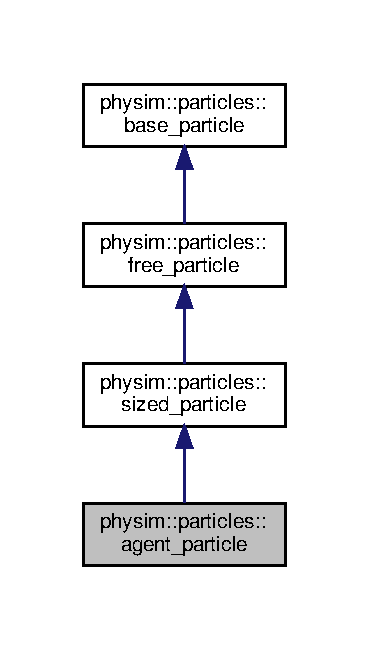
\includegraphics[width=177pt]{classphysim_1_1particles_1_1agent__particle__inherit__graph}
\end{center}
\end{figure}


Collaboration diagram for physim\+:\+:particles\+:\+:agent\+\_\+particle\+:\nopagebreak
\begin{figure}[H]
\begin{center}
\leavevmode
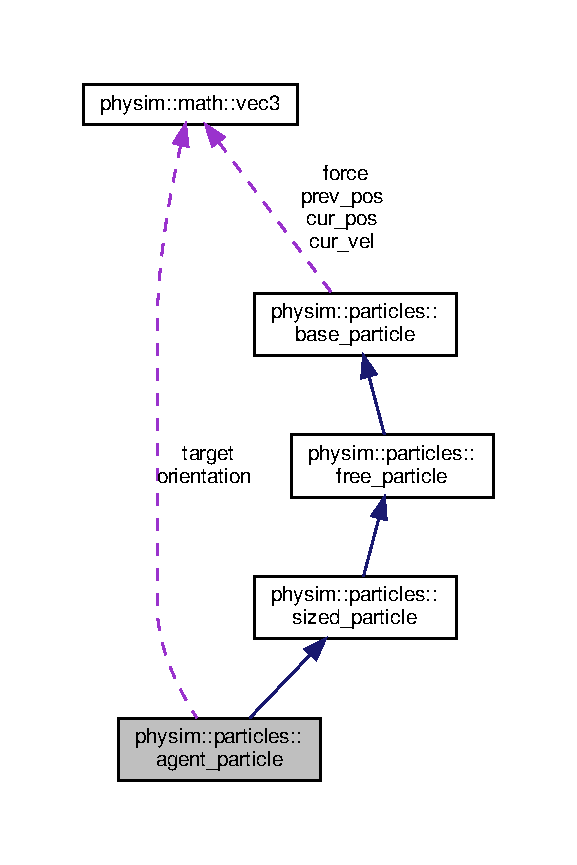
\includegraphics[width=277pt]{classphysim_1_1particles_1_1agent__particle__coll__graph}
\end{center}
\end{figure}
\subsection*{Public Member Functions}
\begin{DoxyCompactItemize}
\item 
\mbox{\Hypertarget{classphysim_1_1particles_1_1agent__particle_aac223ecaf20c17b0ac3198ee1248938c}\label{classphysim_1_1particles_1_1agent__particle_aac223ecaf20c17b0ac3198ee1248938c}} 
\hyperlink{classphysim_1_1particles_1_1agent__particle_aac223ecaf20c17b0ac3198ee1248938c}{agent\+\_\+particle} ()
\begin{DoxyCompactList}\small\item\em Default constructor. \end{DoxyCompactList}\item 
\mbox{\Hypertarget{classphysim_1_1particles_1_1agent__particle_a319cdfd5aeb3dbe7df1d8dade4999db8}\label{classphysim_1_1particles_1_1agent__particle_a319cdfd5aeb3dbe7df1d8dade4999db8}} 
\hyperlink{classphysim_1_1particles_1_1agent__particle_a319cdfd5aeb3dbe7df1d8dade4999db8}{agent\+\_\+particle} (const \hyperlink{classphysim_1_1particles_1_1agent__particle}{agent\+\_\+particle} \&p)
\begin{DoxyCompactList}\small\item\em Copy constructor. \end{DoxyCompactList}\item 
\mbox{\Hypertarget{classphysim_1_1particles_1_1agent__particle_a8198fc4f3f25ece0d43c1ec1ce36ac1c}\label{classphysim_1_1particles_1_1agent__particle_a8198fc4f3f25ece0d43c1ec1ce36ac1c}} 
virtual \hyperlink{classphysim_1_1particles_1_1agent__particle_a8198fc4f3f25ece0d43c1ec1ce36ac1c}{$\sim$agent\+\_\+particle} ()
\begin{DoxyCompactList}\small\item\em Destructor. \end{DoxyCompactList}\item 
void \hyperlink{classphysim_1_1particles_1_1agent__particle_ac13082909f480fc55d406321c77d38b1}{init} ()
\begin{DoxyCompactList}\small\item\em Initialises all particle\textquotesingle{}s attributes, most of them to null values. \end{DoxyCompactList}\item 
\mbox{\Hypertarget{classphysim_1_1particles_1_1agent__particle_aa053f50646658dcb4676a1ffd688a8ce}\label{classphysim_1_1particles_1_1agent__particle_aa053f50646658dcb4676a1ffd688a8ce}} 
virtual \hyperlink{namespacephysim_1_1particles_a068e6cda6626fbd381c07a9835425b08}{particle\+\_\+type} \hyperlink{classphysim_1_1particles_1_1agent__particle_aa053f50646658dcb4676a1ffd688a8ce}{get\+\_\+particle\+\_\+type} () const
\begin{DoxyCompactList}\small\item\em Returns the type of this particle. \end{DoxyCompactList}\item 
\mbox{\Hypertarget{classphysim_1_1particles_1_1agent__particle_a9e8fe0f0491005226f77bdb829132be6}\label{classphysim_1_1particles_1_1agent__particle_a9e8fe0f0491005226f77bdb829132be6}} 
bool \hyperlink{classphysim_1_1particles_1_1agent__particle_a9e8fe0f0491005226f77bdb829132be6}{is\+\_\+behaviour\+\_\+set} (const \hyperlink{namespacephysim_1_1particles_a033757595f7862a0fc8a389d79bf9c88}{agent\+\_\+behaviour\+\_\+type} \&b) const
\begin{DoxyCompactList}\small\item\em Returns whether behaviour {\itshape b} is activated or not. \end{DoxyCompactList}\item 
void \hyperlink{classphysim_1_1particles_1_1agent__particle_a5eeac79c256570806270b4de1907396f}{set\+\_\+behaviour} (const \hyperlink{namespacephysim_1_1particles_a033757595f7862a0fc8a389d79bf9c88}{agent\+\_\+behaviour\+\_\+type} \&b)
\begin{DoxyCompactList}\small\item\em Sets a type of behaviour. \end{DoxyCompactList}\item 
void \hyperlink{classphysim_1_1particles_1_1agent__particle_a903f5a9d1c34eed73dd5286e55e41b3d}{unset\+\_\+behaviour} (const \hyperlink{namespacephysim_1_1particles_a033757595f7862a0fc8a389d79bf9c88}{agent\+\_\+behaviour\+\_\+type} \&b)
\begin{DoxyCompactList}\small\item\em Sets a type of behaviour. \end{DoxyCompactList}\item 
void \hyperlink{classphysim_1_1particles_1_1agent__particle_a1707492909bba01164bf38186a68bcb7}{unset\+\_\+all\+\_\+behaviours} ()
\begin{DoxyCompactList}\small\item\em Unsets all behavours of the agent. \end{DoxyCompactList}\item 
void \hyperlink{classphysim_1_1particles_1_1agent__particle_a8c43ad56e0b73e6795a287fb945da092}{apply\+\_\+behaviours} (\hyperlink{structphysim_1_1math_1_1vec3}{math\+::vec3} \&weighted\+\_\+steering) const
\begin{DoxyCompactList}\small\item\em Computes a weighted steering vector force. \end{DoxyCompactList}\item 
void \hyperlink{classphysim_1_1particles_1_1agent__particle_abd9976b5fd7b03ef4301878085e21fbc}{apply\+\_\+behaviours} (const std\+::vector$<$ \hyperlink{classphysim_1_1geometric_1_1geometry}{geometric\+::geometry} $\ast$$>$ \&scene, \hyperlink{structphysim_1_1math_1_1vec3}{math\+::vec3} \&weighted\+\_\+steering) const
\begin{DoxyCompactList}\small\item\em Computes a weighted steering vector force. \end{DoxyCompactList}\item 
virtual void \hyperlink{classphysim_1_1particles_1_1agent__particle_ac4eabcfb94d1c5769415f8822556be8b}{seek\+\_\+behaviour} (\hyperlink{structphysim_1_1math_1_1vec3}{math\+::vec3} \&v) const
\begin{DoxyCompactList}\small\item\em Computes the seek steering force. \end{DoxyCompactList}\item 
virtual void \hyperlink{classphysim_1_1particles_1_1agent__particle_aca72133a2c84d5849185cbe8daf8910f}{flee\+\_\+behaviour} (\hyperlink{structphysim_1_1math_1_1vec3}{math\+::vec3} \&v) const
\begin{DoxyCompactList}\small\item\em Computes the flee steering force. \end{DoxyCompactList}\item 
virtual void \hyperlink{classphysim_1_1particles_1_1agent__particle_a2859f442bcd33d39767e15d882ba5229}{arrival\+\_\+behaviour} (\hyperlink{structphysim_1_1math_1_1vec3}{math\+::vec3} \&v) const
\begin{DoxyCompactList}\small\item\em Computes the arrival steering force. \end{DoxyCompactList}\item 
virtual void \hyperlink{classphysim_1_1particles_1_1agent__particle_a776246cbbc1550db54368039db73d51b}{collision\+\_\+avoidance\+\_\+behaviour} (const std\+::vector$<$ \hyperlink{classphysim_1_1geometric_1_1geometry}{geometric\+::geometry} $\ast$$>$ \&scene, \hyperlink{structphysim_1_1math_1_1vec3}{math\+::vec3} \&v) const
\begin{DoxyCompactList}\small\item\em Computes the collision avoidance steering force. \end{DoxyCompactList}\end{DoxyCompactItemize}
\subsection*{Public Attributes}
\begin{DoxyCompactItemize}
\item 
\hyperlink{structphysim_1_1math_1_1vec3}{math\+::vec3} \hyperlink{classphysim_1_1particles_1_1agent__particle_a0658207e11a5d39844856233ae8bf2cb}{target}
\begin{DoxyCompactList}\small\item\em Target position of this particle. \end{DoxyCompactList}\item 
\hyperlink{structphysim_1_1math_1_1vec3}{math\+::vec3} \hyperlink{classphysim_1_1particles_1_1agent__particle_a87b2554699454e6850f1d2b48e278f63}{orientation}
\begin{DoxyCompactList}\small\item\em Vector indicating the orientation of the particle. \end{DoxyCompactList}\item 
\mbox{\Hypertarget{classphysim_1_1particles_1_1agent__particle_af219e3f46630bb7f51f3d00952ed4f1c}\label{classphysim_1_1particles_1_1agent__particle_af219e3f46630bb7f51f3d00952ed4f1c}} 
\hyperlink{namespacephysim_1_1particles_a033757595f7862a0fc8a389d79bf9c88}{agent\+\_\+behaviour\+\_\+type} \hyperlink{classphysim_1_1particles_1_1agent__particle_af219e3f46630bb7f51f3d00952ed4f1c}{behaviour}
\begin{DoxyCompactList}\small\item\em Behaviour of this agent. \end{DoxyCompactList}\item 
float \hyperlink{classphysim_1_1particles_1_1agent__particle_a3e34a9a7fc82cbad0226b7b925b5ba22}{max\+\_\+speed}
\begin{DoxyCompactList}\small\item\em Maximum speed allowed. \mbox{[}m/s\mbox{]}. \end{DoxyCompactList}\item 
float \hyperlink{classphysim_1_1particles_1_1agent__particle_a57909cb85564f4432754000ed570d88a}{max\+\_\+force}
\begin{DoxyCompactList}\small\item\em Maximum force allowed. \mbox{[}m/s\mbox{]}. \end{DoxyCompactList}\item 
float \hyperlink{classphysim_1_1particles_1_1agent__particle_a1c3e4357a84047b45ea827a2e90cd14b}{slowing\+\_\+distance}
\begin{DoxyCompactList}\small\item\em Distance from the target to start slowing down at. \end{DoxyCompactList}\item 
\mbox{\Hypertarget{classphysim_1_1particles_1_1agent__particle_a119da4916df4f5c52f13170725295f20}\label{classphysim_1_1particles_1_1agent__particle_a119da4916df4f5c52f13170725295f20}} 
float \hyperlink{classphysim_1_1particles_1_1agent__particle_a119da4916df4f5c52f13170725295f20}{align\+\_\+weight}
\begin{DoxyCompactList}\small\item\em Weight for aligning orientation with velocity. \end{DoxyCompactList}\item 
\mbox{\Hypertarget{classphysim_1_1particles_1_1agent__particle_a853c72c7dbd902a126af1a90d50af222}\label{classphysim_1_1particles_1_1agent__particle_a853c72c7dbd902a126af1a90d50af222}} 
float \hyperlink{classphysim_1_1particles_1_1agent__particle_a853c72c7dbd902a126af1a90d50af222}{seek\+\_\+weight}
\begin{DoxyCompactList}\small\item\em Weight for seek behaviour. \end{DoxyCompactList}\item 
\mbox{\Hypertarget{classphysim_1_1particles_1_1agent__particle_ad7824cd0742b42f803542d8b4d5eae98}\label{classphysim_1_1particles_1_1agent__particle_ad7824cd0742b42f803542d8b4d5eae98}} 
float \hyperlink{classphysim_1_1particles_1_1agent__particle_ad7824cd0742b42f803542d8b4d5eae98}{flee\+\_\+weight}
\begin{DoxyCompactList}\small\item\em Weight for flee behaviour. \end{DoxyCompactList}\item 
\mbox{\Hypertarget{classphysim_1_1particles_1_1agent__particle_aaeb579f8b30b7604d7205bb7aff5197b}\label{classphysim_1_1particles_1_1agent__particle_aaeb579f8b30b7604d7205bb7aff5197b}} 
float \hyperlink{classphysim_1_1particles_1_1agent__particle_aaeb579f8b30b7604d7205bb7aff5197b}{arrival\+\_\+weight}
\begin{DoxyCompactList}\small\item\em Weight for arrival behaviour. \end{DoxyCompactList}\item 
\mbox{\Hypertarget{classphysim_1_1particles_1_1agent__particle_acf2c406d0b41c07d3f786701dec35020}\label{classphysim_1_1particles_1_1agent__particle_acf2c406d0b41c07d3f786701dec35020}} 
float \hyperlink{classphysim_1_1particles_1_1agent__particle_acf2c406d0b41c07d3f786701dec35020}{coll\+\_\+avoid\+\_\+weight}
\begin{DoxyCompactList}\small\item\em Weight for collision avoidance behaviour. \end{DoxyCompactList}\item 
\mbox{\Hypertarget{classphysim_1_1particles_1_1agent__particle_ab08a6b3f3a8f27b3281d981146135234}\label{classphysim_1_1particles_1_1agent__particle_ab08a6b3f3a8f27b3281d981146135234}} 
float \hyperlink{classphysim_1_1particles_1_1agent__particle_ab08a6b3f3a8f27b3281d981146135234}{ahead\+\_\+distance}
\begin{DoxyCompactList}\small\item\em Distance ahead of the agent for collision detection. \end{DoxyCompactList}\end{DoxyCompactItemize}
\subsection*{Private Member Functions}
\begin{DoxyCompactItemize}
\item 
void \hyperlink{classphysim_1_1particles_1_1agent__particle_af48f594a16ab6c2ff3b475fa7f64266c}{partial\+\_\+init} ()
\begin{DoxyCompactList}\small\item\em Initialises this class\textquotesingle{}s attributes. \end{DoxyCompactList}\end{DoxyCompactItemize}


\subsection{Detailed Description}
Class implementing an agent particle. 

An agent particle is useful for defining, using a physically-\/based model, the movement of an agent (say, a human(oid), car, ...) through an environment, in the presence of other agents and obstacles.

Although it is a type of sized particle (see \hyperlink{classphysim_1_1particles_1_1sized__particle}{sized\+\_\+particle}), which in turn is a type of free particle (see \hyperlink{classphysim_1_1particles_1_1free__particle}{free\+\_\+particle}), its starting time (see \hyperlink{classphysim_1_1particles_1_1free__particle_ad0379ba926ecc909bfbfb373045bfcf9}{free\+\_\+particle\+::starttime}) is ignored. Its lifetime, however, it is not (see \hyperlink{classphysim_1_1particles_1_1free__particle_a5870d6fd3167d2c6120f887f45fe50fc}{free\+\_\+particle\+::lifetime}). The simulation of an agent particle depend on its behaviour (see \hyperlink{classphysim_1_1particles_1_1agent__particle_af219e3f46630bb7f51f3d00952ed4f1c}{agent\+\_\+particle\+::behaviour}). 

\subsection{Member Function Documentation}
\mbox{\Hypertarget{classphysim_1_1particles_1_1agent__particle_a8c43ad56e0b73e6795a287fb945da092}\label{classphysim_1_1particles_1_1agent__particle_a8c43ad56e0b73e6795a287fb945da092}} 
\index{physim\+::particles\+::agent\+\_\+particle@{physim\+::particles\+::agent\+\_\+particle}!apply\+\_\+behaviours@{apply\+\_\+behaviours}}
\index{apply\+\_\+behaviours@{apply\+\_\+behaviours}!physim\+::particles\+::agent\+\_\+particle@{physim\+::particles\+::agent\+\_\+particle}}
\subsubsection{\texorpdfstring{apply\+\_\+behaviours()}{apply\_behaviours()}\hspace{0.1cm}{\footnotesize\ttfamily [1/2]}}
{\footnotesize\ttfamily void physim\+::particles\+::agent\+\_\+particle\+::apply\+\_\+behaviours (\begin{DoxyParamCaption}\item[{\hyperlink{structphysim_1_1math_1_1vec3}{math\+::vec3} \&}]{weighted\+\_\+steering }\end{DoxyParamCaption}) const}



Computes a weighted steering vector force. 

This vector is the weighted average over the different steering vectors obtained by the different behaviours activated.

The behaviours considered in this function are\+:
\begin{DoxyItemize}
\item \hyperlink{namespacephysim_1_1particles_a033757595f7862a0fc8a389d79bf9c88ae6f6362248805a36c61d205dbc6f4076}{agent\+\_\+behaviour\+\_\+type\+::seek}
\item \hyperlink{namespacephysim_1_1particles_a033757595f7862a0fc8a389d79bf9c88a918634f9410d3be95b2c6074f18cc62b}{agent\+\_\+behaviour\+\_\+type\+::flee}
\item \hyperlink{namespacephysim_1_1particles_a033757595f7862a0fc8a389d79bf9c88a0d4144ffc7e8e66a72800ea2b4101fd0}{agent\+\_\+behaviour\+\_\+type\+::arrival}
\end{DoxyItemize}

The resulting vector will be accumulated to an internal vector \char`\"{}as is\char`\"{} to make a new velocity vector.

Recall that the target is stored in \hyperlink{classphysim_1_1particles_1_1agent__particle_a0658207e11a5d39844856233ae8bf2cb}{target}. 
\begin{DoxyParams}[1]{Parameters}
\mbox{\tt out}  & {\em weighted\+\_\+steering} & Weighted steering vector. \\
\hline
\end{DoxyParams}
\mbox{\Hypertarget{classphysim_1_1particles_1_1agent__particle_abd9976b5fd7b03ef4301878085e21fbc}\label{classphysim_1_1particles_1_1agent__particle_abd9976b5fd7b03ef4301878085e21fbc}} 
\index{physim\+::particles\+::agent\+\_\+particle@{physim\+::particles\+::agent\+\_\+particle}!apply\+\_\+behaviours@{apply\+\_\+behaviours}}
\index{apply\+\_\+behaviours@{apply\+\_\+behaviours}!physim\+::particles\+::agent\+\_\+particle@{physim\+::particles\+::agent\+\_\+particle}}
\subsubsection{\texorpdfstring{apply\+\_\+behaviours()}{apply\_behaviours()}\hspace{0.1cm}{\footnotesize\ttfamily [2/2]}}
{\footnotesize\ttfamily void physim\+::particles\+::agent\+\_\+particle\+::apply\+\_\+behaviours (\begin{DoxyParamCaption}\item[{const std\+::vector$<$ \hyperlink{classphysim_1_1geometric_1_1geometry}{geometric\+::geometry} $\ast$$>$ \&}]{scene,  }\item[{\hyperlink{structphysim_1_1math_1_1vec3}{math\+::vec3} \&}]{weighted\+\_\+steering }\end{DoxyParamCaption}) const}



Computes a weighted steering vector force. 

This vector is the weighted average over the different steering vectors obtained by the different behaviours activated.

The behaviours considered in this function are\+:
\begin{DoxyItemize}
\item \hyperlink{namespacephysim_1_1particles_a033757595f7862a0fc8a389d79bf9c88aa150bf2057adbf0518b8bd2a4019d5a4}{agent\+\_\+behaviour\+\_\+type\+::collision\+\_\+avoidance}.
\end{DoxyItemize}

This function is called for every geometrical object in the scene. It is up to the user to decide what is a \char`\"{}most threatening\char`\"{} geometrical object.

The resulting vector will be accumulated to an internal vector \char`\"{}as is\char`\"{} to make a new velocity vector.

Recall that the target is stored in \hyperlink{classphysim_1_1particles_1_1agent__particle_a0658207e11a5d39844856233ae8bf2cb}{target}. 
\begin{DoxyParams}[1]{Parameters}
\mbox{\tt in}  & {\em scene} & The geometry in the simulation. \\
\hline
\mbox{\tt out}  & {\em weighted\+\_\+steering} & Weighted steering vector. \\
\hline
\end{DoxyParams}
\mbox{\Hypertarget{classphysim_1_1particles_1_1agent__particle_a2859f442bcd33d39767e15d882ba5229}\label{classphysim_1_1particles_1_1agent__particle_a2859f442bcd33d39767e15d882ba5229}} 
\index{physim\+::particles\+::agent\+\_\+particle@{physim\+::particles\+::agent\+\_\+particle}!arrival\+\_\+behaviour@{arrival\+\_\+behaviour}}
\index{arrival\+\_\+behaviour@{arrival\+\_\+behaviour}!physim\+::particles\+::agent\+\_\+particle@{physim\+::particles\+::agent\+\_\+particle}}
\subsubsection{\texorpdfstring{arrival\+\_\+behaviour()}{arrival\_behaviour()}}
{\footnotesize\ttfamily void physim\+::particles\+::agent\+\_\+particle\+::arrival\+\_\+behaviour (\begin{DoxyParamCaption}\item[{\hyperlink{structphysim_1_1math_1_1vec3}{math\+::vec3} \&}]{v }\end{DoxyParamCaption}) const\hspace{0.3cm}{\ttfamily [virtual]}}



Computes the arrival steering force. 

This function must compute a velocity vector multiplied by a certain weight. The result must be assigned to {\itshape v}.

Recall that the slowing distance considered is stored in {\itshape v}.


\begin{DoxyParams}[1]{Parameters}
\mbox{\tt out}  & {\em v} & Arrival steering vector. \\
\hline
\end{DoxyParams}
\begin{DoxyPrecond}{Precondition}
Vector {\itshape v} may not be initialised to 0. 
\end{DoxyPrecond}
\mbox{\Hypertarget{classphysim_1_1particles_1_1agent__particle_a776246cbbc1550db54368039db73d51b}\label{classphysim_1_1particles_1_1agent__particle_a776246cbbc1550db54368039db73d51b}} 
\index{physim\+::particles\+::agent\+\_\+particle@{physim\+::particles\+::agent\+\_\+particle}!collision\+\_\+avoidance\+\_\+behaviour@{collision\+\_\+avoidance\+\_\+behaviour}}
\index{collision\+\_\+avoidance\+\_\+behaviour@{collision\+\_\+avoidance\+\_\+behaviour}!physim\+::particles\+::agent\+\_\+particle@{physim\+::particles\+::agent\+\_\+particle}}
\subsubsection{\texorpdfstring{collision\+\_\+avoidance\+\_\+behaviour()}{collision\_avoidance\_behaviour()}}
{\footnotesize\ttfamily void physim\+::particles\+::agent\+\_\+particle\+::collision\+\_\+avoidance\+\_\+behaviour (\begin{DoxyParamCaption}\item[{const std\+::vector$<$ \hyperlink{classphysim_1_1geometric_1_1geometry}{geometric\+::geometry} $\ast$$>$ \&}]{scene,  }\item[{\hyperlink{structphysim_1_1math_1_1vec3}{math\+::vec3} \&}]{v }\end{DoxyParamCaption}) const\hspace{0.3cm}{\ttfamily [virtual]}}



Computes the collision avoidance steering force. 

This function must compute a velocity vector multiplied by a certain weight. The result must be assigned to {\itshape v}.

Rectangles are considered walls. The rest of the geometry is approximated with spheres.


\begin{DoxyParams}[1]{Parameters}
\mbox{\tt in}  & {\em scene} & The geometry in the simulation. \\
\hline
\mbox{\tt out}  & {\em v} & Collision avoidance steering vector. \\
\hline
\end{DoxyParams}
\begin{DoxyPrecond}{Precondition}
Vector {\itshape v} may not be initialised to 0. 
\end{DoxyPrecond}
\mbox{\Hypertarget{classphysim_1_1particles_1_1agent__particle_aca72133a2c84d5849185cbe8daf8910f}\label{classphysim_1_1particles_1_1agent__particle_aca72133a2c84d5849185cbe8daf8910f}} 
\index{physim\+::particles\+::agent\+\_\+particle@{physim\+::particles\+::agent\+\_\+particle}!flee\+\_\+behaviour@{flee\+\_\+behaviour}}
\index{flee\+\_\+behaviour@{flee\+\_\+behaviour}!physim\+::particles\+::agent\+\_\+particle@{physim\+::particles\+::agent\+\_\+particle}}
\subsubsection{\texorpdfstring{flee\+\_\+behaviour()}{flee\_behaviour()}}
{\footnotesize\ttfamily void physim\+::particles\+::agent\+\_\+particle\+::flee\+\_\+behaviour (\begin{DoxyParamCaption}\item[{\hyperlink{structphysim_1_1math_1_1vec3}{math\+::vec3} \&}]{v }\end{DoxyParamCaption}) const\hspace{0.3cm}{\ttfamily [virtual]}}



Computes the flee steering force. 

This function must compute a velocity vector multiplied by a certain weight. The result must be assigned to {\itshape v}.


\begin{DoxyParams}[1]{Parameters}
\mbox{\tt out}  & {\em v} & Flee steering vector. \\
\hline
\end{DoxyParams}
\begin{DoxyPrecond}{Precondition}
Vector {\itshape v} may not be initialised to 0. 
\end{DoxyPrecond}
\mbox{\Hypertarget{classphysim_1_1particles_1_1agent__particle_ac13082909f480fc55d406321c77d38b1}\label{classphysim_1_1particles_1_1agent__particle_ac13082909f480fc55d406321c77d38b1}} 
\index{physim\+::particles\+::agent\+\_\+particle@{physim\+::particles\+::agent\+\_\+particle}!init@{init}}
\index{init@{init}!physim\+::particles\+::agent\+\_\+particle@{physim\+::particles\+::agent\+\_\+particle}}
\subsubsection{\texorpdfstring{init()}{init()}}
{\footnotesize\ttfamily void physim\+::particles\+::agent\+\_\+particle\+::init (\begin{DoxyParamCaption}{ }\end{DoxyParamCaption})\hspace{0.3cm}{\ttfamily [virtual]}}



Initialises all particle\textquotesingle{}s attributes, most of them to null values. 

The attributes of the class take the following values\+:
\begin{DoxyItemize}
\item \hyperlink{classphysim_1_1particles_1_1base__particle_a08072db6a1a59d21acc9cac6ac8965f7}{prev\+\_\+pos} \+: vec3(0,0,0)
\item \hyperlink{classphysim_1_1particles_1_1base__particle_a66a164d2a130c40901e3ec2709cdad43}{cur\+\_\+vel} \+: vec3(0,0,0)
\item \hyperlink{classphysim_1_1particles_1_1base__particle_adc3b11899d2e50970ae5d4931721a0ef}{force} \+: vec3(0,0,0)
\item \hyperlink{classphysim_1_1particles_1_1base__particle_acb5c9f0b4a911d8981210e2cfc4dda8a}{mass} \+: 1
\item \hyperlink{classphysim_1_1particles_1_1base__particle_a44f5de3bb4b860dfd511e28e1d6519d5}{index} \+: no value assigned, since it will be overwritten by the simulator.
\item \hyperlink{classphysim_1_1particles_1_1free__particle_aac766fa5294e47b944d32ca3e38d47fa}{bouncing} \+: 0.\+8
\item \hyperlink{classphysim_1_1particles_1_1free__particle_a9e7dfd81e9392fc42b3faecb57afdc02}{friction} \+: 0.\+2
\item \hyperlink{classphysim_1_1particles_1_1free__particle_a7513ac41f3cab1ce083f8695e2c73301}{charge} \+: 0
\item \hyperlink{classphysim_1_1particles_1_1free__particle_a5870d6fd3167d2c6120f887f45fe50fc}{lifetime} \+: 10
\item \hyperlink{classphysim_1_1particles_1_1free__particle_ad0379ba926ecc909bfbfb373045bfcf9}{starttime} \+: 0
\item \hyperlink{classphysim_1_1particles_1_1free__particle_a0f6d69caeac140abd74c7be4ed55eb74}{fixed} \+: false
\item \hyperlink{classphysim_1_1particles_1_1sized__particle_ac67d5df84b91bb12152c8691dd43e98c}{R} \+: 1.\+0
\item \hyperlink{classphysim_1_1particles_1_1agent__particle_a0658207e11a5d39844856233ae8bf2cb}{target} \+: vec3(0,0,0)
\item \hyperlink{classphysim_1_1particles_1_1agent__particle_a87b2554699454e6850f1d2b48e278f63}{orientation} \+: vec3(0,0,0)
\item \hyperlink{classphysim_1_1particles_1_1agent__particle_af219e3f46630bb7f51f3d00952ed4f1c}{behaviour} \+: \hyperlink{namespacephysim_1_1particles_a033757595f7862a0fc8a389d79bf9c88a334c4a4c42fdb79d7ebc3e73b517e6f8}{agent\+\_\+behaviour\+\_\+type\+::none}
\item \hyperlink{classphysim_1_1particles_1_1agent__particle_a3e34a9a7fc82cbad0226b7b925b5ba22}{max\+\_\+speed} \+: 1.\+0
\item \hyperlink{classphysim_1_1particles_1_1agent__particle_a57909cb85564f4432754000ed570d88a}{max\+\_\+force} \+: 1.\+0
\item \hyperlink{classphysim_1_1particles_1_1agent__particle_a1c3e4357a84047b45ea827a2e90cd14b}{slowing\+\_\+distance} \+: 0.\+0
\item \hyperlink{classphysim_1_1particles_1_1agent__particle_a119da4916df4f5c52f13170725295f20}{align\+\_\+weight} \+: 1.\+0/5.0
\item \hyperlink{classphysim_1_1particles_1_1agent__particle_a853c72c7dbd902a126af1a90d50af222}{seek\+\_\+weight} \+: 1.\+0/5.0
\item \hyperlink{classphysim_1_1particles_1_1agent__particle_ad7824cd0742b42f803542d8b4d5eae98}{flee\+\_\+weight} \+: 1.\+0/5.0
\item \hyperlink{classphysim_1_1particles_1_1agent__particle_aaeb579f8b30b7604d7205bb7aff5197b}{arrival\+\_\+weight} \+: 1.\+0/5.0
\item \hyperlink{classphysim_1_1particles_1_1agent__particle_acf2c406d0b41c07d3f786701dec35020}{coll\+\_\+avoid\+\_\+weight} \+: 1.\+0/5.0
\item \hyperlink{classphysim_1_1particles_1_1agent__particle_ab08a6b3f3a8f27b3281d981146135234}{ahead\+\_\+distance} \+: 5.\+0 
\end{DoxyItemize}

Reimplemented from \hyperlink{classphysim_1_1particles_1_1free__particle_a0df21e64a28c5fdf471d54a50b59fea3}{physim\+::particles\+::free\+\_\+particle}.

\mbox{\Hypertarget{classphysim_1_1particles_1_1agent__particle_af48f594a16ab6c2ff3b475fa7f64266c}\label{classphysim_1_1particles_1_1agent__particle_af48f594a16ab6c2ff3b475fa7f64266c}} 
\index{physim\+::particles\+::agent\+\_\+particle@{physim\+::particles\+::agent\+\_\+particle}!partial\+\_\+init@{partial\+\_\+init}}
\index{partial\+\_\+init@{partial\+\_\+init}!physim\+::particles\+::agent\+\_\+particle@{physim\+::particles\+::agent\+\_\+particle}}
\subsubsection{\texorpdfstring{partial\+\_\+init()}{partial\_init()}}
{\footnotesize\ttfamily void physim\+::particles\+::agent\+\_\+particle\+::partial\+\_\+init (\begin{DoxyParamCaption}{ }\end{DoxyParamCaption})\hspace{0.3cm}{\ttfamily [private]}}



Initialises this class\textquotesingle{}s attributes. 

The attributes of the class take the following values\+:
\begin{DoxyItemize}
\item \hyperlink{classphysim_1_1particles_1_1agent__particle_a0658207e11a5d39844856233ae8bf2cb}{target} \+: vec3(0,0,0)
\item \hyperlink{classphysim_1_1particles_1_1agent__particle_a87b2554699454e6850f1d2b48e278f63}{orientation} \+: vec3(0,0,0)
\item \hyperlink{classphysim_1_1particles_1_1agent__particle_af219e3f46630bb7f51f3d00952ed4f1c}{behaviour} \+: \hyperlink{namespacephysim_1_1particles_a033757595f7862a0fc8a389d79bf9c88a334c4a4c42fdb79d7ebc3e73b517e6f8}{agent\+\_\+behaviour\+\_\+type\+::none}
\item \hyperlink{classphysim_1_1particles_1_1agent__particle_a3e34a9a7fc82cbad0226b7b925b5ba22}{max\+\_\+speed} \+: 1.\+0
\item \hyperlink{classphysim_1_1particles_1_1agent__particle_a57909cb85564f4432754000ed570d88a}{max\+\_\+force} \+: 1.\+0
\item \hyperlink{classphysim_1_1particles_1_1agent__particle_a1c3e4357a84047b45ea827a2e90cd14b}{slowing\+\_\+distance} \+: 0.\+0
\item \hyperlink{classphysim_1_1particles_1_1agent__particle_a119da4916df4f5c52f13170725295f20}{align\+\_\+weight} \+: 1.\+0/5.0
\item \hyperlink{classphysim_1_1particles_1_1agent__particle_a853c72c7dbd902a126af1a90d50af222}{seek\+\_\+weight} \+: 1.\+0/5.0
\item \hyperlink{classphysim_1_1particles_1_1agent__particle_ad7824cd0742b42f803542d8b4d5eae98}{flee\+\_\+weight} \+: 1.\+0/5.0
\item \hyperlink{classphysim_1_1particles_1_1agent__particle_aaeb579f8b30b7604d7205bb7aff5197b}{arrival\+\_\+weight} \+: 1.\+0/5.0
\item \hyperlink{classphysim_1_1particles_1_1agent__particle_acf2c406d0b41c07d3f786701dec35020}{coll\+\_\+avoid\+\_\+weight} \+: 1.\+0/5.0
\item \hyperlink{classphysim_1_1particles_1_1agent__particle_ab08a6b3f3a8f27b3281d981146135234}{ahead\+\_\+distance} \+: 5.\+0 
\end{DoxyItemize}\mbox{\Hypertarget{classphysim_1_1particles_1_1agent__particle_ac4eabcfb94d1c5769415f8822556be8b}\label{classphysim_1_1particles_1_1agent__particle_ac4eabcfb94d1c5769415f8822556be8b}} 
\index{physim\+::particles\+::agent\+\_\+particle@{physim\+::particles\+::agent\+\_\+particle}!seek\+\_\+behaviour@{seek\+\_\+behaviour}}
\index{seek\+\_\+behaviour@{seek\+\_\+behaviour}!physim\+::particles\+::agent\+\_\+particle@{physim\+::particles\+::agent\+\_\+particle}}
\subsubsection{\texorpdfstring{seek\+\_\+behaviour()}{seek\_behaviour()}}
{\footnotesize\ttfamily void physim\+::particles\+::agent\+\_\+particle\+::seek\+\_\+behaviour (\begin{DoxyParamCaption}\item[{\hyperlink{structphysim_1_1math_1_1vec3}{math\+::vec3} \&}]{v }\end{DoxyParamCaption}) const\hspace{0.3cm}{\ttfamily [virtual]}}



Computes the seek steering force. 

This function must compute a velocity vector multiplied by a certain weight. The result must be assigned to {\itshape v}.


\begin{DoxyParams}[1]{Parameters}
\mbox{\tt out}  & {\em v} & Seek steering vector. \\
\hline
\end{DoxyParams}
\begin{DoxyPrecond}{Precondition}
Vector {\itshape v} may not be initialised to 0. 
\end{DoxyPrecond}
\mbox{\Hypertarget{classphysim_1_1particles_1_1agent__particle_a5eeac79c256570806270b4de1907396f}\label{classphysim_1_1particles_1_1agent__particle_a5eeac79c256570806270b4de1907396f}} 
\index{physim\+::particles\+::agent\+\_\+particle@{physim\+::particles\+::agent\+\_\+particle}!set\+\_\+behaviour@{set\+\_\+behaviour}}
\index{set\+\_\+behaviour@{set\+\_\+behaviour}!physim\+::particles\+::agent\+\_\+particle@{physim\+::particles\+::agent\+\_\+particle}}
\subsubsection{\texorpdfstring{set\+\_\+behaviour()}{set\_behaviour()}}
{\footnotesize\ttfamily void physim\+::particles\+::agent\+\_\+particle\+::set\+\_\+behaviour (\begin{DoxyParamCaption}\item[{const \hyperlink{namespacephysim_1_1particles_a033757595f7862a0fc8a389d79bf9c88}{agent\+\_\+behaviour\+\_\+type} \&}]{b }\end{DoxyParamCaption})}



Sets a type of behaviour. 

Attribute \hyperlink{classphysim_1_1particles_1_1agent__particle_af219e3f46630bb7f51f3d00952ed4f1c}{behaviour} is modified so that the evaluation of \begin{DoxyVerb}behaviour | b
\end{DoxyVerb}
 results to a value different from 0, where {\itshape b} is the behaviour type passed as parameter. 
\begin{DoxyParams}{Parameters}
{\em b} & Type of behaviour. \\
\hline
\end{DoxyParams}
\mbox{\Hypertarget{classphysim_1_1particles_1_1agent__particle_a1707492909bba01164bf38186a68bcb7}\label{classphysim_1_1particles_1_1agent__particle_a1707492909bba01164bf38186a68bcb7}} 
\index{physim\+::particles\+::agent\+\_\+particle@{physim\+::particles\+::agent\+\_\+particle}!unset\+\_\+all\+\_\+behaviours@{unset\+\_\+all\+\_\+behaviours}}
\index{unset\+\_\+all\+\_\+behaviours@{unset\+\_\+all\+\_\+behaviours}!physim\+::particles\+::agent\+\_\+particle@{physim\+::particles\+::agent\+\_\+particle}}
\subsubsection{\texorpdfstring{unset\+\_\+all\+\_\+behaviours()}{unset\_all\_behaviours()}}
{\footnotesize\ttfamily void physim\+::particles\+::agent\+\_\+particle\+::unset\+\_\+all\+\_\+behaviours (\begin{DoxyParamCaption}{ }\end{DoxyParamCaption})}



Unsets all behavours of the agent. 

Sets its behaviour to \hyperlink{namespacephysim_1_1particles_a033757595f7862a0fc8a389d79bf9c88a334c4a4c42fdb79d7ebc3e73b517e6f8}{agent\+\_\+behaviour\+\_\+type\+::none}. \mbox{\Hypertarget{classphysim_1_1particles_1_1agent__particle_a903f5a9d1c34eed73dd5286e55e41b3d}\label{classphysim_1_1particles_1_1agent__particle_a903f5a9d1c34eed73dd5286e55e41b3d}} 
\index{physim\+::particles\+::agent\+\_\+particle@{physim\+::particles\+::agent\+\_\+particle}!unset\+\_\+behaviour@{unset\+\_\+behaviour}}
\index{unset\+\_\+behaviour@{unset\+\_\+behaviour}!physim\+::particles\+::agent\+\_\+particle@{physim\+::particles\+::agent\+\_\+particle}}
\subsubsection{\texorpdfstring{unset\+\_\+behaviour()}{unset\_behaviour()}}
{\footnotesize\ttfamily void physim\+::particles\+::agent\+\_\+particle\+::unset\+\_\+behaviour (\begin{DoxyParamCaption}\item[{const \hyperlink{namespacephysim_1_1particles_a033757595f7862a0fc8a389d79bf9c88}{agent\+\_\+behaviour\+\_\+type} \&}]{b }\end{DoxyParamCaption})}



Sets a type of behaviour. 

Attribute \hyperlink{classphysim_1_1particles_1_1agent__particle_af219e3f46630bb7f51f3d00952ed4f1c}{behaviour} is modified so that the evaluation of \begin{DoxyVerb}behaviour | b
\end{DoxyVerb}
 results to a value equal to 0, where {\itshape b} is the behaviour type passed as parameter. 
\begin{DoxyParams}{Parameters}
{\em b} & Type of behaviour. \\
\hline
\end{DoxyParams}


\subsection{Member Data Documentation}
\mbox{\Hypertarget{classphysim_1_1particles_1_1agent__particle_a57909cb85564f4432754000ed570d88a}\label{classphysim_1_1particles_1_1agent__particle_a57909cb85564f4432754000ed570d88a}} 
\index{physim\+::particles\+::agent\+\_\+particle@{physim\+::particles\+::agent\+\_\+particle}!max\+\_\+force@{max\+\_\+force}}
\index{max\+\_\+force@{max\+\_\+force}!physim\+::particles\+::agent\+\_\+particle@{physim\+::particles\+::agent\+\_\+particle}}
\subsubsection{\texorpdfstring{max\+\_\+force}{max\_force}}
{\footnotesize\ttfamily float physim\+::particles\+::agent\+\_\+particle\+::max\+\_\+force}



Maximum force allowed. \mbox{[}m/s\mbox{]}. 

This particle can move at a velocity with maximum magnitude stored in this value. \mbox{\Hypertarget{classphysim_1_1particles_1_1agent__particle_a3e34a9a7fc82cbad0226b7b925b5ba22}\label{classphysim_1_1particles_1_1agent__particle_a3e34a9a7fc82cbad0226b7b925b5ba22}} 
\index{physim\+::particles\+::agent\+\_\+particle@{physim\+::particles\+::agent\+\_\+particle}!max\+\_\+speed@{max\+\_\+speed}}
\index{max\+\_\+speed@{max\+\_\+speed}!physim\+::particles\+::agent\+\_\+particle@{physim\+::particles\+::agent\+\_\+particle}}
\subsubsection{\texorpdfstring{max\+\_\+speed}{max\_speed}}
{\footnotesize\ttfamily float physim\+::particles\+::agent\+\_\+particle\+::max\+\_\+speed}



Maximum speed allowed. \mbox{[}m/s\mbox{]}. 

This particle can move at a velocity with maximum magnitude stored in this value. \mbox{\Hypertarget{classphysim_1_1particles_1_1agent__particle_a87b2554699454e6850f1d2b48e278f63}\label{classphysim_1_1particles_1_1agent__particle_a87b2554699454e6850f1d2b48e278f63}} 
\index{physim\+::particles\+::agent\+\_\+particle@{physim\+::particles\+::agent\+\_\+particle}!orientation@{orientation}}
\index{orientation@{orientation}!physim\+::particles\+::agent\+\_\+particle@{physim\+::particles\+::agent\+\_\+particle}}
\subsubsection{\texorpdfstring{orientation}{orientation}}
{\footnotesize\ttfamily \hyperlink{structphysim_1_1math_1_1vec3}{math\+::vec3} physim\+::particles\+::agent\+\_\+particle\+::orientation}



Vector indicating the orientation of the particle. 

This need not be equal to the \hyperlink{classphysim_1_1particles_1_1base__particle_a66a164d2a130c40901e3ec2709cdad43}{cur\+\_\+vel} vector, but it should be initialised with a value equal to the velocity. \mbox{\Hypertarget{classphysim_1_1particles_1_1agent__particle_a1c3e4357a84047b45ea827a2e90cd14b}\label{classphysim_1_1particles_1_1agent__particle_a1c3e4357a84047b45ea827a2e90cd14b}} 
\index{physim\+::particles\+::agent\+\_\+particle@{physim\+::particles\+::agent\+\_\+particle}!slowing\+\_\+distance@{slowing\+\_\+distance}}
\index{slowing\+\_\+distance@{slowing\+\_\+distance}!physim\+::particles\+::agent\+\_\+particle@{physim\+::particles\+::agent\+\_\+particle}}
\subsubsection{\texorpdfstring{slowing\+\_\+distance}{slowing\_distance}}
{\footnotesize\ttfamily float physim\+::particles\+::agent\+\_\+particle\+::slowing\+\_\+distance}



Distance from the target to start slowing down at. 

When the agent is in behaviour arrival (see \hyperlink{namespacephysim_1_1particles_a033757595f7862a0fc8a389d79bf9c88a0d4144ffc7e8e66a72800ea2b4101fd0}{agent\+\_\+behaviour\+\_\+type\+::arrival}) it starts slow down. This attribute encodes the distance from its target at which this happens. \mbox{\Hypertarget{classphysim_1_1particles_1_1agent__particle_a0658207e11a5d39844856233ae8bf2cb}\label{classphysim_1_1particles_1_1agent__particle_a0658207e11a5d39844856233ae8bf2cb}} 
\index{physim\+::particles\+::agent\+\_\+particle@{physim\+::particles\+::agent\+\_\+particle}!target@{target}}
\index{target@{target}!physim\+::particles\+::agent\+\_\+particle@{physim\+::particles\+::agent\+\_\+particle}}
\subsubsection{\texorpdfstring{target}{target}}
{\footnotesize\ttfamily \hyperlink{structphysim_1_1math_1_1vec3}{math\+::vec3} physim\+::particles\+::agent\+\_\+particle\+::target}



Target position of this particle. 

A target is a position this agent particle will want to move to or away from. This will depend on the behaviour of this particle. See \hyperlink{classphysim_1_1particles_1_1agent__particle_af219e3f46630bb7f51f3d00952ed4f1c}{behaviour}. 

The documentation for this class was generated from the following files\+:\begin{DoxyCompactItemize}
\item 
physim/particles/agent\+\_\+particle.\+hpp\item 
physim/particles/agent\+\_\+particle.\+cpp\end{DoxyCompactItemize}

\hypertarget{classphysim_1_1emitters_1_1base__emitter}{}\section{physim\+:\+:emitters\+:\+:base\+\_\+emitter Class Reference}
\label{classphysim_1_1emitters_1_1base__emitter}\index{physim\+::emitters\+::base\+\_\+emitter@{physim\+::emitters\+::base\+\_\+emitter}}


Class for particle initialisation.  




{\ttfamily \#include $<$base\+\_\+emitter.\+hpp$>$}



Inheritance diagram for physim\+:\+:emitters\+:\+:base\+\_\+emitter\+:\nopagebreak
\begin{figure}[H]
\begin{center}
\leavevmode
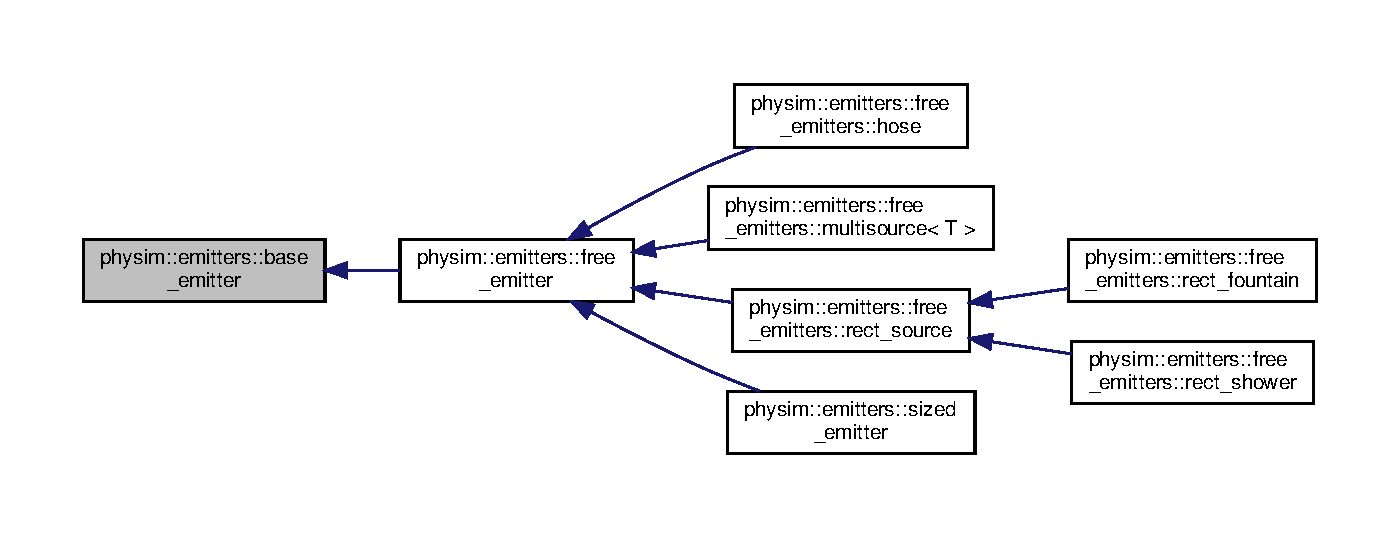
\includegraphics[width=350pt]{classphysim_1_1emitters_1_1base__emitter__inherit__graph}
\end{center}
\end{figure}
\subsection*{Public Member Functions}
\begin{DoxyCompactItemize}
\item 
\mbox{\Hypertarget{classphysim_1_1emitters_1_1base__emitter_a1ba00208368aa0ecc74a8656f48f34fe}\label{classphysim_1_1emitters_1_1base__emitter_a1ba00208368aa0ecc74a8656f48f34fe}} 
\hyperlink{classphysim_1_1emitters_1_1base__emitter_a1ba00208368aa0ecc74a8656f48f34fe}{base\+\_\+emitter} ()
\begin{DoxyCompactList}\small\item\em Default constructor. \end{DoxyCompactList}\item 
\mbox{\Hypertarget{classphysim_1_1emitters_1_1base__emitter_a4ad1e29d66eeee4c5497a6094a538687}\label{classphysim_1_1emitters_1_1base__emitter_a4ad1e29d66eeee4c5497a6094a538687}} 
\hyperlink{classphysim_1_1emitters_1_1base__emitter_a4ad1e29d66eeee4c5497a6094a538687}{base\+\_\+emitter} (const \hyperlink{classphysim_1_1emitters_1_1base__emitter}{base\+\_\+emitter} \&i)
\begin{DoxyCompactList}\small\item\em Copy constructor. \end{DoxyCompactList}\item 
\mbox{\Hypertarget{classphysim_1_1emitters_1_1base__emitter_a9c85997b84bc4e4df420a0cdb01f9ca7}\label{classphysim_1_1emitters_1_1base__emitter_a9c85997b84bc4e4df420a0cdb01f9ca7}} 
virtual \hyperlink{classphysim_1_1emitters_1_1base__emitter_a9c85997b84bc4e4df420a0cdb01f9ca7}{$\sim$base\+\_\+emitter} ()
\begin{DoxyCompactList}\small\item\em Destructor. \end{DoxyCompactList}\item 
\mbox{\Hypertarget{classphysim_1_1emitters_1_1base__emitter_ae04c07cfff6bf1fa2c3b49a0ea1b418a}\label{classphysim_1_1emitters_1_1base__emitter_ae04c07cfff6bf1fa2c3b49a0ea1b418a}} 
void \hyperlink{classphysim_1_1emitters_1_1base__emitter_ae04c07cfff6bf1fa2c3b49a0ea1b418a}{set\+\_\+pos\+\_\+initialiser} (const \hyperlink{namespacephysim_1_1emitters_affb35fbd5f02c488436287899e35d4aa}{base\+\_\+emit} \&f)
\begin{DoxyCompactList}\small\item\em Sets the position emitter\+\_\+base. See \hyperlink{classphysim_1_1emitters_1_1base__emitter_ac67584a2ca34232c1f4f04c41599df0e}{pos}. \end{DoxyCompactList}\item 
\mbox{\Hypertarget{classphysim_1_1emitters_1_1base__emitter_a4e68e1abb0a3a2a007c27208ecfb8aa4}\label{classphysim_1_1emitters_1_1base__emitter_a4e68e1abb0a3a2a007c27208ecfb8aa4}} 
void \hyperlink{classphysim_1_1emitters_1_1base__emitter_a4e68e1abb0a3a2a007c27208ecfb8aa4}{set\+\_\+vel\+\_\+initialiser} (const \hyperlink{namespacephysim_1_1emitters_affb35fbd5f02c488436287899e35d4aa}{base\+\_\+emit} \&f)
\begin{DoxyCompactList}\small\item\em Sets the velocity emitter\+\_\+base. See \hyperlink{classphysim_1_1emitters_1_1base__emitter_a9ea19d96450cff65882371b61a2294c8}{vel}. \end{DoxyCompactList}\item 
\mbox{\Hypertarget{classphysim_1_1emitters_1_1base__emitter_a976d6168972637d231b5fff89f78c55a}\label{classphysim_1_1emitters_1_1base__emitter_a976d6168972637d231b5fff89f78c55a}} 
void \hyperlink{classphysim_1_1emitters_1_1base__emitter_a976d6168972637d231b5fff89f78c55a}{set\+\_\+mass\+\_\+initialiser} (const \hyperlink{namespacephysim_1_1emitters_affb35fbd5f02c488436287899e35d4aa}{base\+\_\+emit} \&f)
\begin{DoxyCompactList}\small\item\em Sets the mass emitter\+\_\+base. See \hyperlink{classphysim_1_1emitters_1_1base__emitter_a4e1b65730afef86899544d3306f7547d}{mass}. \end{DoxyCompactList}\item 
\mbox{\Hypertarget{classphysim_1_1emitters_1_1base__emitter_ab97486c7e3855fca1f08eedbb97c8c0e}\label{classphysim_1_1emitters_1_1base__emitter_ab97486c7e3855fca1f08eedbb97c8c0e}} 
virtual \hyperlink{classphysim_1_1emitters_1_1base__emitter}{base\+\_\+emitter} $\ast$ \hyperlink{classphysim_1_1emitters_1_1base__emitter_ab97486c7e3855fca1f08eedbb97c8c0e}{clone} () const
\begin{DoxyCompactList}\small\item\em Returns a reference to a copy of this emitter\+\_\+base. \end{DoxyCompactList}\item 
\mbox{\Hypertarget{classphysim_1_1emitters_1_1base__emitter_a2dfeb7d710cfae879185548cbd9c4104}\label{classphysim_1_1emitters_1_1base__emitter_a2dfeb7d710cfae879185548cbd9c4104}} 
const \hyperlink{namespacephysim_1_1emitters_affb35fbd5f02c488436287899e35d4aa}{base\+\_\+emit} \& \hyperlink{classphysim_1_1emitters_1_1base__emitter_a2dfeb7d710cfae879185548cbd9c4104}{get\+\_\+pos\+\_\+initialiser} () const
\begin{DoxyCompactList}\small\item\em Returns the position emitter\+\_\+base. See \hyperlink{classphysim_1_1emitters_1_1base__emitter_ac67584a2ca34232c1f4f04c41599df0e}{pos}. \end{DoxyCompactList}\item 
\mbox{\Hypertarget{classphysim_1_1emitters_1_1base__emitter_a9487c303b322b6cbbdff0a8f955effa5}\label{classphysim_1_1emitters_1_1base__emitter_a9487c303b322b6cbbdff0a8f955effa5}} 
const \hyperlink{namespacephysim_1_1emitters_affb35fbd5f02c488436287899e35d4aa}{base\+\_\+emit} \& \hyperlink{classphysim_1_1emitters_1_1base__emitter_a9487c303b322b6cbbdff0a8f955effa5}{get\+\_\+vel\+\_\+initialiser} () const
\begin{DoxyCompactList}\small\item\em Returns the velocity emitter\+\_\+base. See \hyperlink{classphysim_1_1emitters_1_1base__emitter_a9ea19d96450cff65882371b61a2294c8}{vel}. \end{DoxyCompactList}\item 
\mbox{\Hypertarget{classphysim_1_1emitters_1_1base__emitter_a59a316ddacdea8ed05f79e06f3238f4a}\label{classphysim_1_1emitters_1_1base__emitter_a59a316ddacdea8ed05f79e06f3238f4a}} 
const \hyperlink{namespacephysim_1_1emitters_affb35fbd5f02c488436287899e35d4aa}{base\+\_\+emit} \& \hyperlink{classphysim_1_1emitters_1_1base__emitter_a59a316ddacdea8ed05f79e06f3238f4a}{get\+\_\+mass\+\_\+initialiser} () const
\begin{DoxyCompactList}\small\item\em Returns the mass emitter\+\_\+base. See \hyperlink{classphysim_1_1emitters_1_1base__emitter_a4e1b65730afef86899544d3306f7547d}{mass}. \end{DoxyCompactList}\item 
void \hyperlink{classphysim_1_1emitters_1_1base__emitter_a8549c2d921e3a47d15705a6143527ca2}{initialise\+\_\+particle} (\hyperlink{classphysim_1_1particles_1_1base__particle}{particles\+::base\+\_\+particle} \&p) const
\begin{DoxyCompactList}\small\item\em Initialise a particle. \end{DoxyCompactList}\end{DoxyCompactItemize}
\subsection*{Protected Attributes}
\begin{DoxyCompactItemize}
\item 
\mbox{\Hypertarget{classphysim_1_1emitters_1_1base__emitter_ac67584a2ca34232c1f4f04c41599df0e}\label{classphysim_1_1emitters_1_1base__emitter_ac67584a2ca34232c1f4f04c41599df0e}} 
\hyperlink{namespacephysim_1_1emitters_affb35fbd5f02c488436287899e35d4aa}{base\+\_\+emit} \hyperlink{classphysim_1_1emitters_1_1base__emitter_ac67584a2ca34232c1f4f04c41599df0e}{pos}
\begin{DoxyCompactList}\small\item\em Initialiser of position. \end{DoxyCompactList}\item 
\mbox{\Hypertarget{classphysim_1_1emitters_1_1base__emitter_a9ea19d96450cff65882371b61a2294c8}\label{classphysim_1_1emitters_1_1base__emitter_a9ea19d96450cff65882371b61a2294c8}} 
\hyperlink{namespacephysim_1_1emitters_affb35fbd5f02c488436287899e35d4aa}{base\+\_\+emit} \hyperlink{classphysim_1_1emitters_1_1base__emitter_a9ea19d96450cff65882371b61a2294c8}{vel}
\begin{DoxyCompactList}\small\item\em Initialiser of velocity. \end{DoxyCompactList}\item 
\mbox{\Hypertarget{classphysim_1_1emitters_1_1base__emitter_a4e1b65730afef86899544d3306f7547d}\label{classphysim_1_1emitters_1_1base__emitter_a4e1b65730afef86899544d3306f7547d}} 
\hyperlink{namespacephysim_1_1emitters_affb35fbd5f02c488436287899e35d4aa}{base\+\_\+emit} \hyperlink{classphysim_1_1emitters_1_1base__emitter_a4e1b65730afef86899544d3306f7547d}{mass}
\begin{DoxyCompactList}\small\item\em Initialiser of the mass. \end{DoxyCompactList}\end{DoxyCompactItemize}


\subsection{Detailed Description}
Class for particle initialisation. 

This class is used to initialise the attributes of a particle.

This class has several functions as attributes, each of which initialises an attribute of the particle.

These functions are\+:
\begin{DoxyItemize}
\item \hyperlink{classphysim_1_1emitters_1_1base__emitter_ac67584a2ca34232c1f4f04c41599df0e}{pos} \+: function used to initialise the position of a particle.
\item \hyperlink{classphysim_1_1emitters_1_1base__emitter_a9ea19d96450cff65882371b61a2294c8}{vel} \+: function used to initialise the velocity of a particle.
\item \hyperlink{classphysim_1_1emitters_1_1base__emitter_a4e1b65730afef86899544d3306f7547d}{mass} \+: function to initialise the mass of the particle. this function is used to initialse the radius attribute of the particle).
\end{DoxyItemize}

By default, all these function\textquotesingle{}s behaviour is to initialise a particle the same way they are initialised when constructed (see \hyperlink{classphysim_1_1particles_1_1base__particle_a3bba517d51fd0bff7ec583e701765f87}{base\+\_\+particle\+::init}).

Also, they are applied in the same order as they appear listed. Therefore, for example, the position attributes can be used to initialise the velocity. Finally, it is guaranteed that all these functions will be called after the \hyperlink{classphysim_1_1simulator}{simulator} has assigned an index to the particle being initialised.

The previous position of a particle is updated automatically after initialising all attributes using the functions, but on the simulator. Therefore, there is no need to initialise it.

The initialisation of the particle takes place in the method \hyperlink{classphysim_1_1emitters_1_1base__emitter_a8549c2d921e3a47d15705a6143527ca2}{initialise\+\_\+particle(base\+\_\+particle\&)const}.

Finally, all classes must implement the \hyperlink{classphysim_1_1emitters_1_1base__emitter_ab97486c7e3855fca1f08eedbb97c8c0e}{clone} function. 

\subsection{Member Function Documentation}
\mbox{\Hypertarget{classphysim_1_1emitters_1_1base__emitter_a8549c2d921e3a47d15705a6143527ca2}\label{classphysim_1_1emitters_1_1base__emitter_a8549c2d921e3a47d15705a6143527ca2}} 
\index{physim\+::emitters\+::base\+\_\+emitter@{physim\+::emitters\+::base\+\_\+emitter}!initialise\+\_\+particle@{initialise\+\_\+particle}}
\index{initialise\+\_\+particle@{initialise\+\_\+particle}!physim\+::emitters\+::base\+\_\+emitter@{physim\+::emitters\+::base\+\_\+emitter}}
\subsubsection{\texorpdfstring{initialise\+\_\+particle()}{initialise\_particle()}}
{\footnotesize\ttfamily void physim\+::emitters\+::base\+\_\+emitter\+::initialise\+\_\+particle (\begin{DoxyParamCaption}\item[{\hyperlink{classphysim_1_1particles_1_1base__particle}{particles\+::base\+\_\+particle} \&}]{p }\end{DoxyParamCaption}) const}



Initialise a particle. 

Each of the functions for particle initialisation are called on the particle. For details on the order, see the description of this class. 
\begin{DoxyParams}{Parameters}
{\em p} & The particle to be initialised. \\
\hline
\end{DoxyParams}


The documentation for this class was generated from the following files\+:\begin{DoxyCompactItemize}
\item 
physim/emitter/base\+\_\+emitter.\+hpp\item 
physim/emitter/base\+\_\+emitter.\+cpp\end{DoxyCompactItemize}

\hypertarget{classphysim_1_1particles_1_1base__particle}{}\section{physim\+:\+:particles\+:\+:base\+\_\+particle Class Reference}
\label{classphysim_1_1particles_1_1base__particle}\index{physim\+::particles\+::base\+\_\+particle@{physim\+::particles\+::base\+\_\+particle}}


Class implementing the most basic particle.  




{\ttfamily \#include $<$base\+\_\+particle.\+hpp$>$}



Inheritance diagram for physim\+:\+:particles\+:\+:base\+\_\+particle\+:\nopagebreak
\begin{figure}[H]
\begin{center}
\leavevmode
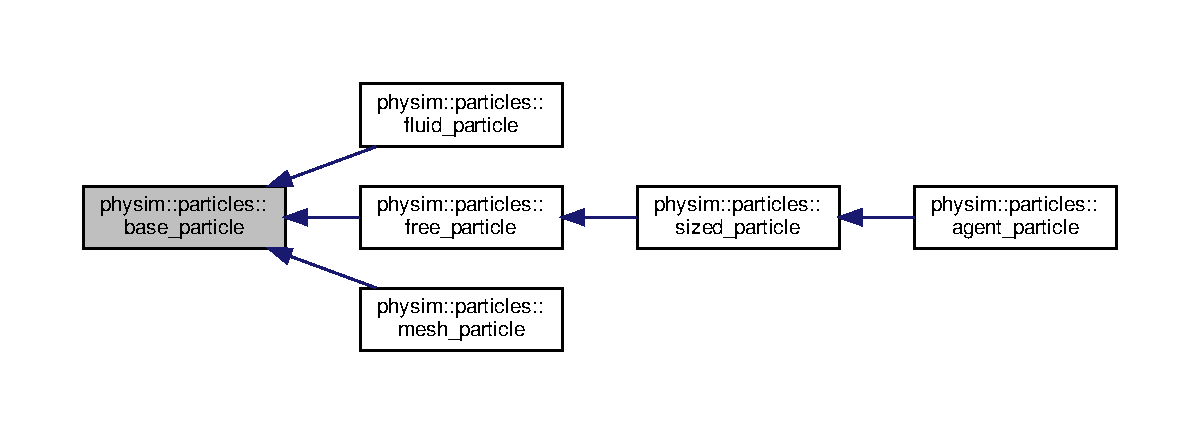
\includegraphics[width=350pt]{classphysim_1_1particles_1_1base__particle__inherit__graph}
\end{center}
\end{figure}


Collaboration diagram for physim\+:\+:particles\+:\+:base\+\_\+particle\+:\nopagebreak
\begin{figure}[H]
\begin{center}
\leavevmode
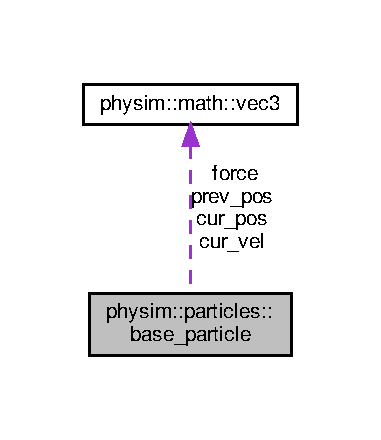
\includegraphics[width=183pt]{classphysim_1_1particles_1_1base__particle__coll__graph}
\end{center}
\end{figure}
\subsection*{Public Member Functions}
\begin{DoxyCompactItemize}
\item 
\mbox{\Hypertarget{classphysim_1_1particles_1_1base__particle_ad42844e13e91c175c3911439a0e08940}\label{classphysim_1_1particles_1_1base__particle_ad42844e13e91c175c3911439a0e08940}} 
\hyperlink{classphysim_1_1particles_1_1base__particle_ad42844e13e91c175c3911439a0e08940}{base\+\_\+particle} ()
\begin{DoxyCompactList}\small\item\em Default constructor. \end{DoxyCompactList}\item 
\mbox{\Hypertarget{classphysim_1_1particles_1_1base__particle_a3055f0439b30d31a94f0e2b3fc0300d0}\label{classphysim_1_1particles_1_1base__particle_a3055f0439b30d31a94f0e2b3fc0300d0}} 
\hyperlink{classphysim_1_1particles_1_1base__particle_a3055f0439b30d31a94f0e2b3fc0300d0}{base\+\_\+particle} (const \hyperlink{classphysim_1_1particles_1_1base__particle}{base\+\_\+particle} \&p)
\begin{DoxyCompactList}\small\item\em Copy constructor. \end{DoxyCompactList}\item 
\mbox{\Hypertarget{classphysim_1_1particles_1_1base__particle_a41ef26ded7282647f2dbe576714f6a4f}\label{classphysim_1_1particles_1_1base__particle_a41ef26ded7282647f2dbe576714f6a4f}} 
virtual \hyperlink{classphysim_1_1particles_1_1base__particle_a41ef26ded7282647f2dbe576714f6a4f}{$\sim$base\+\_\+particle} ()
\begin{DoxyCompactList}\small\item\em Destructor. \end{DoxyCompactList}\item 
void \hyperlink{classphysim_1_1particles_1_1base__particle_aee1ed4e0daca8db01c3a8f150fcdbbb1}{save\+\_\+position} ()
\begin{DoxyCompactList}\small\item\em Saves the current position in the particle\textquotesingle{}s state. \end{DoxyCompactList}\item 
virtual void \hyperlink{classphysim_1_1particles_1_1base__particle_a3bba517d51fd0bff7ec583e701765f87}{init} ()
\begin{DoxyCompactList}\small\item\em Initialises all particle\textquotesingle{}s attributes, most of them to null values. \end{DoxyCompactList}\item 
\mbox{\Hypertarget{classphysim_1_1particles_1_1base__particle_ac6aec0759a48d4337006aa41c280b8fc}\label{classphysim_1_1particles_1_1base__particle_ac6aec0759a48d4337006aa41c280b8fc}} 
virtual \hyperlink{namespacephysim_1_1particles_a068e6cda6626fbd381c07a9835425b08}{particle\+\_\+type} \hyperlink{classphysim_1_1particles_1_1base__particle_ac6aec0759a48d4337006aa41c280b8fc}{get\+\_\+particle\+\_\+type} () const
\begin{DoxyCompactList}\small\item\em Returns the type of this particle. \end{DoxyCompactList}\end{DoxyCompactItemize}
\subsection*{Public Attributes}
\begin{DoxyCompactItemize}
\item 
\mbox{\Hypertarget{classphysim_1_1particles_1_1base__particle_a08072db6a1a59d21acc9cac6ac8965f7}\label{classphysim_1_1particles_1_1base__particle_a08072db6a1a59d21acc9cac6ac8965f7}} 
\hyperlink{structphysim_1_1math_1_1vec3}{math\+::vec3} \hyperlink{classphysim_1_1particles_1_1base__particle_a08072db6a1a59d21acc9cac6ac8965f7}{prev\+\_\+pos}
\begin{DoxyCompactList}\small\item\em Previous position of the particle \mbox{[}m\mbox{]}. \end{DoxyCompactList}\item 
\mbox{\Hypertarget{classphysim_1_1particles_1_1base__particle_a6298a121dea043741e5d3722386163c6}\label{classphysim_1_1particles_1_1base__particle_a6298a121dea043741e5d3722386163c6}} 
\hyperlink{structphysim_1_1math_1_1vec3}{math\+::vec3} \hyperlink{classphysim_1_1particles_1_1base__particle_a6298a121dea043741e5d3722386163c6}{cur\+\_\+pos}
\begin{DoxyCompactList}\small\item\em Current position of the particle \mbox{[}m\mbox{]}. \end{DoxyCompactList}\item 
\mbox{\Hypertarget{classphysim_1_1particles_1_1base__particle_a66a164d2a130c40901e3ec2709cdad43}\label{classphysim_1_1particles_1_1base__particle_a66a164d2a130c40901e3ec2709cdad43}} 
\hyperlink{structphysim_1_1math_1_1vec3}{math\+::vec3} \hyperlink{classphysim_1_1particles_1_1base__particle_a66a164d2a130c40901e3ec2709cdad43}{cur\+\_\+vel}
\begin{DoxyCompactList}\small\item\em Current velocity of the particle \mbox{[}m/s\mbox{]}. \end{DoxyCompactList}\item 
\mbox{\Hypertarget{classphysim_1_1particles_1_1base__particle_adc3b11899d2e50970ae5d4931721a0ef}\label{classphysim_1_1particles_1_1base__particle_adc3b11899d2e50970ae5d4931721a0ef}} 
\hyperlink{structphysim_1_1math_1_1vec3}{math\+::vec3} \hyperlink{classphysim_1_1particles_1_1base__particle_adc3b11899d2e50970ae5d4931721a0ef}{force}
\begin{DoxyCompactList}\small\item\em Force currently applied to the particle \mbox{[}N\mbox{]}. \end{DoxyCompactList}\item 
\mbox{\Hypertarget{classphysim_1_1particles_1_1base__particle_acb5c9f0b4a911d8981210e2cfc4dda8a}\label{classphysim_1_1particles_1_1base__particle_acb5c9f0b4a911d8981210e2cfc4dda8a}} 
float \hyperlink{classphysim_1_1particles_1_1base__particle_acb5c9f0b4a911d8981210e2cfc4dda8a}{mass}
\begin{DoxyCompactList}\small\item\em Mass of the particle \mbox{[}Kg\mbox{]}. \end{DoxyCompactList}\item 
size\+\_\+t \hyperlink{classphysim_1_1particles_1_1base__particle_a44f5de3bb4b860dfd511e28e1d6519d5}{index}
\begin{DoxyCompactList}\small\item\em Index of the particle. \end{DoxyCompactList}\end{DoxyCompactItemize}


\subsection{Detailed Description}
Class implementing the most basic particle. 

The most basic particle in this library is a 0-\/dimensional object that is subject to several forces but not to any other particle\textquotesingle{}s direct interaction through them. It can collide with other objects in the scene (geometrical objects, see namespace \hyperlink{namespacephysim_1_1geometric}{physim\+::geometric}) and maybe with other particles, depending on the subclass. 

\subsection{Member Function Documentation}
\mbox{\Hypertarget{classphysim_1_1particles_1_1base__particle_a3bba517d51fd0bff7ec583e701765f87}\label{classphysim_1_1particles_1_1base__particle_a3bba517d51fd0bff7ec583e701765f87}} 
\index{physim\+::particles\+::base\+\_\+particle@{physim\+::particles\+::base\+\_\+particle}!init@{init}}
\index{init@{init}!physim\+::particles\+::base\+\_\+particle@{physim\+::particles\+::base\+\_\+particle}}
\subsubsection{\texorpdfstring{init()}{init()}}
{\footnotesize\ttfamily void physim\+::particles\+::base\+\_\+particle\+::init (\begin{DoxyParamCaption}{ }\end{DoxyParamCaption})\hspace{0.3cm}{\ttfamily [virtual]}}



Initialises all particle\textquotesingle{}s attributes, most of them to null values. 

The attributes of the class take the following values\+:
\begin{DoxyItemize}
\item \hyperlink{classphysim_1_1particles_1_1base__particle_a08072db6a1a59d21acc9cac6ac8965f7}{prev\+\_\+pos} \+: vec3(0,0,0)
\item \hyperlink{classphysim_1_1particles_1_1base__particle_a6298a121dea043741e5d3722386163c6}{cur\+\_\+pos} \+: vec3(0,0,0)
\item \hyperlink{classphysim_1_1particles_1_1base__particle_a66a164d2a130c40901e3ec2709cdad43}{cur\+\_\+vel} \+: vec3(0,0,0)
\item \hyperlink{classphysim_1_1particles_1_1base__particle_adc3b11899d2e50970ae5d4931721a0ef}{force} \+: vec3(0,0,0)
\item \hyperlink{classphysim_1_1particles_1_1base__particle_acb5c9f0b4a911d8981210e2cfc4dda8a}{mass} \+: 1
\item \hyperlink{classphysim_1_1particles_1_1base__particle_a44f5de3bb4b860dfd511e28e1d6519d5}{index} \+: no value assigned, since it will be overwritten by the simulator. 
\end{DoxyItemize}

Reimplemented in \hyperlink{classphysim_1_1particles_1_1agent__particle_ac13082909f480fc55d406321c77d38b1}{physim\+::particles\+::agent\+\_\+particle}, \hyperlink{classphysim_1_1particles_1_1free__particle_a0df21e64a28c5fdf471d54a50b59fea3}{physim\+::particles\+::free\+\_\+particle}, \hyperlink{classphysim_1_1particles_1_1mesh__particle_a1b3c3eac1e62296c2facd8c9d9b84608}{physim\+::particles\+::mesh\+\_\+particle}, \hyperlink{classphysim_1_1particles_1_1sized__particle_a63de84961417c1522c0ca576697cd972}{physim\+::particles\+::sized\+\_\+particle}, and \hyperlink{classphysim_1_1particles_1_1fluid__particle_a0aa522f9400bcb02373edd7bb073249b}{physim\+::particles\+::fluid\+\_\+particle}.

\mbox{\Hypertarget{classphysim_1_1particles_1_1base__particle_aee1ed4e0daca8db01c3a8f150fcdbbb1}\label{classphysim_1_1particles_1_1base__particle_aee1ed4e0daca8db01c3a8f150fcdbbb1}} 
\index{physim\+::particles\+::base\+\_\+particle@{physim\+::particles\+::base\+\_\+particle}!save\+\_\+position@{save\+\_\+position}}
\index{save\+\_\+position@{save\+\_\+position}!physim\+::particles\+::base\+\_\+particle@{physim\+::particles\+::base\+\_\+particle}}
\subsubsection{\texorpdfstring{save\+\_\+position()}{save\_position()}}
{\footnotesize\ttfamily void physim\+::particles\+::base\+\_\+particle\+::save\+\_\+position (\begin{DoxyParamCaption}{ }\end{DoxyParamCaption})}



Saves the current position in the particle\textquotesingle{}s state. 

Copies \hyperlink{classphysim_1_1particles_1_1base__particle_a6298a121dea043741e5d3722386163c6}{cur\+\_\+pos} into \hyperlink{classphysim_1_1particles_1_1base__particle_a08072db6a1a59d21acc9cac6ac8965f7}{prev\+\_\+pos}. 

\subsection{Member Data Documentation}
\mbox{\Hypertarget{classphysim_1_1particles_1_1base__particle_a44f5de3bb4b860dfd511e28e1d6519d5}\label{classphysim_1_1particles_1_1base__particle_a44f5de3bb4b860dfd511e28e1d6519d5}} 
\index{physim\+::particles\+::base\+\_\+particle@{physim\+::particles\+::base\+\_\+particle}!index@{index}}
\index{index@{index}!physim\+::particles\+::base\+\_\+particle@{physim\+::particles\+::base\+\_\+particle}}
\subsubsection{\texorpdfstring{index}{index}}
{\footnotesize\ttfamily size\+\_\+t physim\+::particles\+::base\+\_\+particle\+::index}



Index of the particle. 

This index is automatically set when added to the simulator object. The collection of indexes determine the order in which particles have been added to it. The indexes start at 0.

It can be used to initialise its attributes through the different initialiser functions. 

The documentation for this class was generated from the following files\+:\begin{DoxyCompactItemize}
\item 
physim/particles/base\+\_\+particle.\+hpp\item 
physim/particles/base\+\_\+particle.\+cpp\end{DoxyCompactItemize}

\hypertarget{classphysim_1_1fields_1_1field}{}\section{physim\+:\+:fields\+:\+:field Class Reference}
\label{classphysim_1_1fields_1_1field}\index{physim\+::fields\+::field@{physim\+::fields\+::field}}


Abstract class for force fields.  




{\ttfamily \#include $<$field.\+hpp$>$}



Inheritance diagram for physim\+:\+:fields\+:\+:field\+:\nopagebreak
\begin{figure}[H]
\begin{center}
\leavevmode
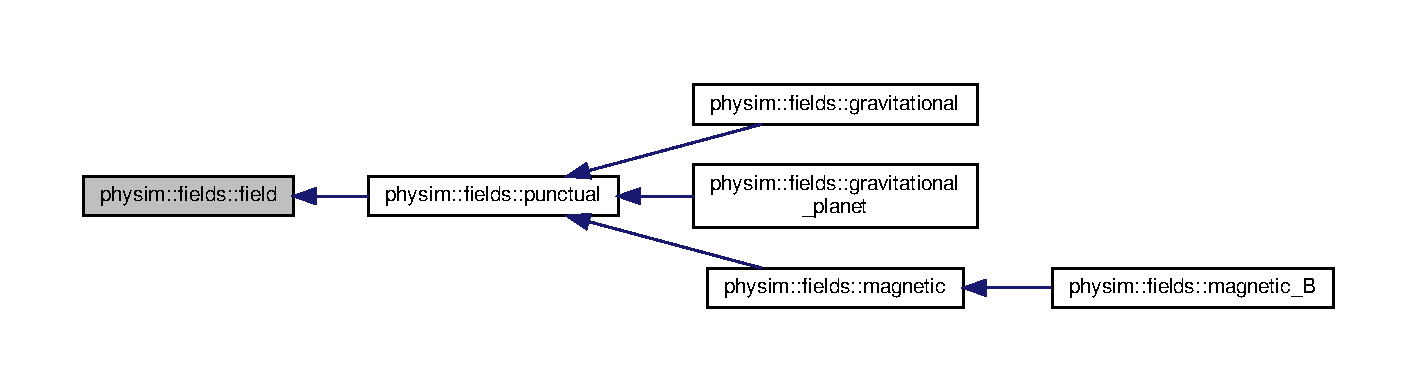
\includegraphics[width=350pt]{classphysim_1_1fields_1_1field__inherit__graph}
\end{center}
\end{figure}
\subsection*{Public Member Functions}
\begin{DoxyCompactItemize}
\item 
\mbox{\Hypertarget{classphysim_1_1fields_1_1field_a2c4e1ea6c27e745695af1cb3fadf9fb6}\label{classphysim_1_1fields_1_1field_a2c4e1ea6c27e745695af1cb3fadf9fb6}} 
\hyperlink{classphysim_1_1fields_1_1field_a2c4e1ea6c27e745695af1cb3fadf9fb6}{field} ()
\begin{DoxyCompactList}\small\item\em Default constructor. \end{DoxyCompactList}\item 
\mbox{\Hypertarget{classphysim_1_1fields_1_1field_ab355221b0b90b4612529c31190cf138f}\label{classphysim_1_1fields_1_1field_ab355221b0b90b4612529c31190cf138f}} 
\hyperlink{classphysim_1_1fields_1_1field_ab355221b0b90b4612529c31190cf138f}{field} (const \hyperlink{classphysim_1_1fields_1_1field}{field} \&f)
\begin{DoxyCompactList}\small\item\em Copy constructor. \end{DoxyCompactList}\item 
\mbox{\Hypertarget{classphysim_1_1fields_1_1field_a296551790d51e6366f3ee608b8505599}\label{classphysim_1_1fields_1_1field_a296551790d51e6366f3ee608b8505599}} 
virtual \hyperlink{classphysim_1_1fields_1_1field_a296551790d51e6366f3ee608b8505599}{$\sim$field} ()
\begin{DoxyCompactList}\small\item\em Destructor. \end{DoxyCompactList}\item 
virtual void \hyperlink{classphysim_1_1fields_1_1field_a0d836756ac51a6a1e99d3c9a60310694}{compute\+\_\+force} (const \hyperlink{classphysim_1_1particles_1_1free__particle}{particles\+::free\+\_\+particle} \&p, \hyperlink{structphysim_1_1math_1_1vec3}{math\+::vec3} \&F)=0
\begin{DoxyCompactList}\small\item\em Compute the force vector acting on a particle. \end{DoxyCompactList}\item 
virtual void \hyperlink{classphysim_1_1fields_1_1field_aa167d81f223daab47989168c9d3b8cb4}{compute\+\_\+force} (const \hyperlink{classphysim_1_1particles_1_1mesh__particle}{particles\+::mesh\+\_\+particle} \&p, \hyperlink{structphysim_1_1math_1_1vec3}{math\+::vec3} \&F)=0
\begin{DoxyCompactList}\small\item\em Compute the force vector acting on a particle. \end{DoxyCompactList}\item 
virtual void \hyperlink{classphysim_1_1fields_1_1field_a099fb8b1dee7afae4610c6275432bc81}{compute\+\_\+force} (const \hyperlink{classphysim_1_1particles_1_1fluid__particle}{particles\+::fluid\+\_\+particle} \&p, \hyperlink{structphysim_1_1math_1_1vec3}{math\+::vec3} \&F)=0
\begin{DoxyCompactList}\small\item\em Compute the force vector acting on a particle. \end{DoxyCompactList}\end{DoxyCompactItemize}


\subsection{Detailed Description}
Abstract class for force fields. 

Any force field is interpreted as a vector field\+: given a position from the field\textquotesingle{}s source there is a force vector that affects a particle in that position.

The source is usually regarded as punctual, i.\+e., the origin of the field is a point. However, this is considered as a type of field, and is implemented in class \hyperlink{classphysim_1_1fields_1_1punctual}{fields\+::punctual}. 

\subsection{Member Function Documentation}
\mbox{\Hypertarget{classphysim_1_1fields_1_1field_a0d836756ac51a6a1e99d3c9a60310694}\label{classphysim_1_1fields_1_1field_a0d836756ac51a6a1e99d3c9a60310694}} 
\index{physim\+::fields\+::field@{physim\+::fields\+::field}!compute\+\_\+force@{compute\+\_\+force}}
\index{compute\+\_\+force@{compute\+\_\+force}!physim\+::fields\+::field@{physim\+::fields\+::field}}
\subsubsection{\texorpdfstring{compute\+\_\+force()}{compute\_force()}\hspace{0.1cm}{\footnotesize\ttfamily [1/3]}}
{\footnotesize\ttfamily virtual void physim\+::fields\+::field\+::compute\+\_\+force (\begin{DoxyParamCaption}\item[{const \hyperlink{classphysim_1_1particles_1_1free__particle}{particles\+::free\+\_\+particle} \&}]{p,  }\item[{\hyperlink{structphysim_1_1math_1_1vec3}{math\+::vec3} \&}]{F }\end{DoxyParamCaption})\hspace{0.3cm}{\ttfamily [pure virtual]}}



Compute the force vector acting on a particle. 

The contents of parameter {\itshape F} is undefined when calling this function, thus the contents should be overwritten. 
\begin{DoxyParams}[1]{Parameters}
\mbox{\tt in}  & {\em p} & Particle where the force is applied to. \\
\hline
\mbox{\tt out}  & {\em F} & The force from this field acting on the particle. \\
\hline
\end{DoxyParams}


Implemented in \hyperlink{classphysim_1_1fields_1_1gravitational_af852abc69f07c67eb888fac9e7637693}{physim\+::fields\+::gravitational}, \hyperlink{classphysim_1_1fields_1_1gravitational__planet_ab272f7db84ad53d320d467b75d3f9ed2}{physim\+::fields\+::gravitational\+\_\+planet}, and \hyperlink{classphysim_1_1fields_1_1magnetic__B_a806a3e8aa306f0ed33954d79c3082698}{physim\+::fields\+::magnetic\+\_\+B}.

\mbox{\Hypertarget{classphysim_1_1fields_1_1field_aa167d81f223daab47989168c9d3b8cb4}\label{classphysim_1_1fields_1_1field_aa167d81f223daab47989168c9d3b8cb4}} 
\index{physim\+::fields\+::field@{physim\+::fields\+::field}!compute\+\_\+force@{compute\+\_\+force}}
\index{compute\+\_\+force@{compute\+\_\+force}!physim\+::fields\+::field@{physim\+::fields\+::field}}
\subsubsection{\texorpdfstring{compute\+\_\+force()}{compute\_force()}\hspace{0.1cm}{\footnotesize\ttfamily [2/3]}}
{\footnotesize\ttfamily virtual void physim\+::fields\+::field\+::compute\+\_\+force (\begin{DoxyParamCaption}\item[{const \hyperlink{classphysim_1_1particles_1_1mesh__particle}{particles\+::mesh\+\_\+particle} \&}]{p,  }\item[{\hyperlink{structphysim_1_1math_1_1vec3}{math\+::vec3} \&}]{F }\end{DoxyParamCaption})\hspace{0.3cm}{\ttfamily [pure virtual]}}



Compute the force vector acting on a particle. 

The contents of parameter {\itshape F} is undefined when calling this function, thus the contents should be overwritten. 
\begin{DoxyParams}[1]{Parameters}
\mbox{\tt in}  & {\em p} & Particle where the force is applied to. \\
\hline
\mbox{\tt out}  & {\em F} & The force from this field acting on the particle. \\
\hline
\end{DoxyParams}


Implemented in \hyperlink{classphysim_1_1fields_1_1gravitational_a2283f98ad0ce6732c81e744d3c2b898d}{physim\+::fields\+::gravitational}, \hyperlink{classphysim_1_1fields_1_1gravitational__planet_aece6e4cc8679b3be5075c1e5fd1b3162}{physim\+::fields\+::gravitational\+\_\+planet}, and \hyperlink{classphysim_1_1fields_1_1magnetic__B_aa337b83c6dea0726d2dc2d7cd1cd978a}{physim\+::fields\+::magnetic\+\_\+B}.

\mbox{\Hypertarget{classphysim_1_1fields_1_1field_a099fb8b1dee7afae4610c6275432bc81}\label{classphysim_1_1fields_1_1field_a099fb8b1dee7afae4610c6275432bc81}} 
\index{physim\+::fields\+::field@{physim\+::fields\+::field}!compute\+\_\+force@{compute\+\_\+force}}
\index{compute\+\_\+force@{compute\+\_\+force}!physim\+::fields\+::field@{physim\+::fields\+::field}}
\subsubsection{\texorpdfstring{compute\+\_\+force()}{compute\_force()}\hspace{0.1cm}{\footnotesize\ttfamily [3/3]}}
{\footnotesize\ttfamily virtual void physim\+::fields\+::field\+::compute\+\_\+force (\begin{DoxyParamCaption}\item[{const \hyperlink{classphysim_1_1particles_1_1fluid__particle}{particles\+::fluid\+\_\+particle} \&}]{p,  }\item[{\hyperlink{structphysim_1_1math_1_1vec3}{math\+::vec3} \&}]{F }\end{DoxyParamCaption})\hspace{0.3cm}{\ttfamily [pure virtual]}}



Compute the force vector acting on a particle. 

The contents of parameter {\itshape F} is undefined when calling this function, thus the contents should be overwritten. 
\begin{DoxyParams}[1]{Parameters}
\mbox{\tt in}  & {\em p} & Particle where the force is applied to. \\
\hline
\mbox{\tt out}  & {\em F} & The force from this field acting on the particle. \\
\hline
\end{DoxyParams}


Implemented in \hyperlink{classphysim_1_1fields_1_1gravitational_a1b11432dfb9e1bc2720794304f224432}{physim\+::fields\+::gravitational}, \hyperlink{classphysim_1_1fields_1_1gravitational__planet_a3b79869e1411c333b21ba4a240574641}{physim\+::fields\+::gravitational\+\_\+planet}, and \hyperlink{classphysim_1_1fields_1_1magnetic__B_a17ca2b3c6cbf61c53665cf23632187b8}{physim\+::fields\+::magnetic\+\_\+B}.



The documentation for this class was generated from the following files\+:\begin{DoxyCompactItemize}
\item 
physim/fields/field.\+hpp\item 
physim/fields/field.\+cpp\end{DoxyCompactItemize}

\hypertarget{classphysim_1_1fluids_1_1fluid}{}\section{physim\+:\+:fluids\+:\+:fluid Class Reference}
\label{classphysim_1_1fluids_1_1fluid}\index{physim\+::fluids\+::fluid@{physim\+::fluids\+::fluid}}


Class implementing a fluid.  




{\ttfamily \#include $<$fluid.\+hpp$>$}



Inheritance diagram for physim\+:\+:fluids\+:\+:fluid\+:\nopagebreak
\begin{figure}[H]
\begin{center}
\leavevmode
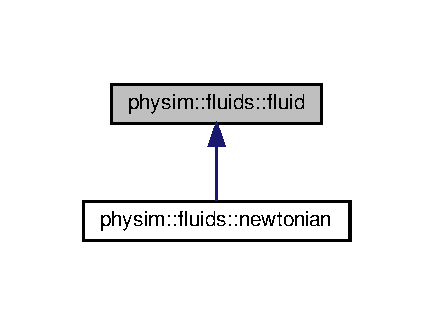
\includegraphics[width=208pt]{classphysim_1_1fluids_1_1fluid__inherit__graph}
\end{center}
\end{figure}


Collaboration diagram for physim\+:\+:fluids\+:\+:fluid\+:\nopagebreak
\begin{figure}[H]
\begin{center}
\leavevmode
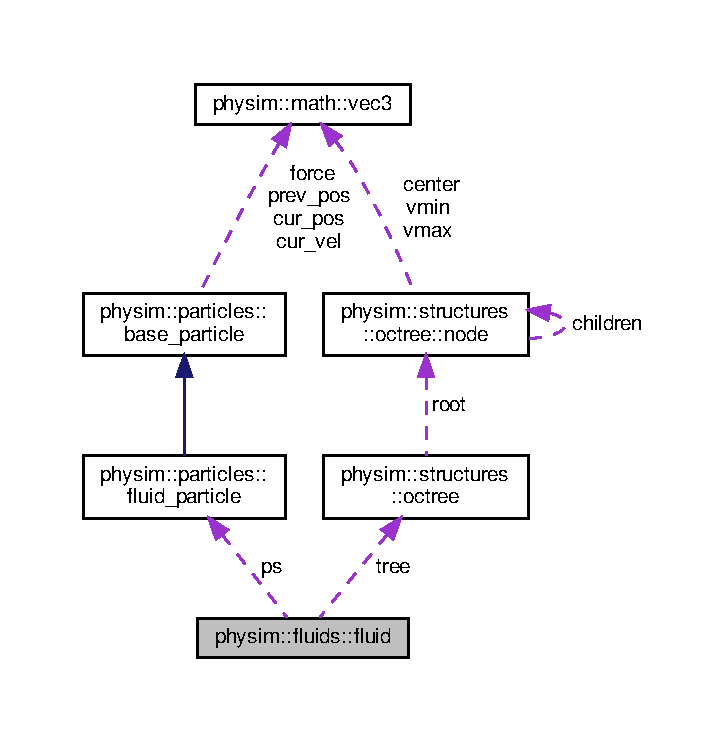
\includegraphics[width=349pt]{classphysim_1_1fluids_1_1fluid__coll__graph}
\end{center}
\end{figure}
\subsection*{Public Member Functions}
\begin{DoxyCompactItemize}
\item 
\mbox{\Hypertarget{classphysim_1_1fluids_1_1fluid_accaba6072529138d6ba9d167ea4febbf}\label{classphysim_1_1fluids_1_1fluid_accaba6072529138d6ba9d167ea4febbf}} 
\hyperlink{classphysim_1_1fluids_1_1fluid_accaba6072529138d6ba9d167ea4febbf}{fluid} ()
\begin{DoxyCompactList}\small\item\em Default onstructor. \end{DoxyCompactList}\item 
\mbox{\Hypertarget{classphysim_1_1fluids_1_1fluid_ad4e5dc8a4530a41727958ad689ce83fb}\label{classphysim_1_1fluids_1_1fluid_ad4e5dc8a4530a41727958ad689ce83fb}} 
virtual \hyperlink{classphysim_1_1fluids_1_1fluid_ad4e5dc8a4530a41727958ad689ce83fb}{$\sim$fluid} ()
\begin{DoxyCompactList}\small\item\em Destructor. \end{DoxyCompactList}\item 
\mbox{\Hypertarget{classphysim_1_1fluids_1_1fluid_ac26ad353b668110caa4328aa3b2a9208}\label{classphysim_1_1fluids_1_1fluid_ac26ad353b668110caa4328aa3b2a9208}} 
\hyperlink{classphysim_1_1particles_1_1fluid__particle}{particles\+::fluid\+\_\+particle} $\ast$ \hyperlink{classphysim_1_1fluids_1_1fluid_ac26ad353b668110caa4328aa3b2a9208}{operator\mbox{[}$\,$\mbox{]}} (size\+\_\+t i)
\begin{DoxyCompactList}\small\item\em Returns a reference to the {\itshape i-\/th} particle. \end{DoxyCompactList}\item 
\mbox{\Hypertarget{classphysim_1_1fluids_1_1fluid_a3e7640bf098662ce95378649eb43c016}\label{classphysim_1_1fluids_1_1fluid_a3e7640bf098662ce95378649eb43c016}} 
const \hyperlink{classphysim_1_1particles_1_1fluid__particle}{particles\+::fluid\+\_\+particle} $\ast$ \hyperlink{classphysim_1_1fluids_1_1fluid_a3e7640bf098662ce95378649eb43c016}{operator\mbox{[}$\,$\mbox{]}} (size\+\_\+t i) const
\begin{DoxyCompactList}\small\item\em Returns a constant reference to the {\itshape i-\/th} particle. \end{DoxyCompactList}\item 
void \hyperlink{classphysim_1_1fluids_1_1fluid_a1572bdeaca8942347aa79ee35a112ce6}{allocate} (size\+\_\+t n, float vol, float dens, float visc, float r, float cs)
\begin{DoxyCompactList}\small\item\em Allocates memoery for {\itshape n} particles. \end{DoxyCompactList}\item 
\mbox{\Hypertarget{classphysim_1_1fluids_1_1fluid_a581b8991d4fd6564c5e0b2a49cacd69c}\label{classphysim_1_1fluids_1_1fluid_a581b8991d4fd6564c5e0b2a49cacd69c}} 
virtual void \hyperlink{classphysim_1_1fluids_1_1fluid_a581b8991d4fd6564c5e0b2a49cacd69c}{clear} ()
\begin{DoxyCompactList}\small\item\em Deallocates the memory occupied by the particles of this fluid. \end{DoxyCompactList}\item 
virtual void \hyperlink{classphysim_1_1fluids_1_1fluid_a6cde063d44b1e33199c08e64d801bb04}{update\+\_\+forces} ()=0
\begin{DoxyCompactList}\small\item\em Update the forces generated within the fluid. \end{DoxyCompactList}\item 
virtual void \hyperlink{classphysim_1_1fluids_1_1fluid_a08fe6b6111608b3deb3c3ddd84e1ab32}{update\+\_\+forces} (size\+\_\+t n)=0
\begin{DoxyCompactList}\small\item\em Update the forces generated within the fluid. \end{DoxyCompactList}\item 
void \hyperlink{classphysim_1_1fluids_1_1fluid_a06bb3b5ad3676e0e8485cba3ca12cd73}{make\+\_\+partition} ()
\begin{DoxyCompactList}\small\item\em Builds the space partition of this fluid\textquotesingle{}s particles. \end{DoxyCompactList}\item 
void \hyperlink{classphysim_1_1fluids_1_1fluid_a5701d069c23eb7a902fa944af1e55b61}{set\+\_\+kernel\+\_\+density} (const \hyperlink{namespacephysim_1_1fluids_a22c55c76ab3fe3de79dada15e2f9c2d6}{kernel\+\_\+scalar\+\_\+function} \&W\+\_\+d)
\begin{DoxyCompactList}\small\item\em Sets the kernel density functions. \end{DoxyCompactList}\item 
void \hyperlink{classphysim_1_1fluids_1_1fluid_ad7cbaf969b9c5e4c75606e2f84b81e69}{set\+\_\+kernel\+\_\+pressure} (const \hyperlink{namespacephysim_1_1fluids_ab109a55050c62abe9c1c23924f620754}{kernel\+\_\+vectorial\+\_\+function} \&W\+\_\+p)
\begin{DoxyCompactList}\small\item\em Sets the kernel pressure functions. \end{DoxyCompactList}\item 
void \hyperlink{classphysim_1_1fluids_1_1fluid_a57d90a54268e6c204e0173f81a678dd6}{set\+\_\+kernel\+\_\+viscosity} (const \hyperlink{namespacephysim_1_1fluids_a22c55c76ab3fe3de79dada15e2f9c2d6}{kernel\+\_\+scalar\+\_\+function} \&W\+\_\+v)
\begin{DoxyCompactList}\small\item\em Sets the kernel viscosity functions. \end{DoxyCompactList}\item 
\mbox{\Hypertarget{classphysim_1_1fluids_1_1fluid_afd3bc254d3c033f42dabd68140b3462f}\label{classphysim_1_1fluids_1_1fluid_afd3bc254d3c033f42dabd68140b3462f}} 
size\+\_\+t \hyperlink{classphysim_1_1fluids_1_1fluid_afd3bc254d3c033f42dabd68140b3462f}{size} () const
\begin{DoxyCompactList}\small\item\em Returns the number of particles. \end{DoxyCompactList}\item 
\mbox{\Hypertarget{classphysim_1_1fluids_1_1fluid_a5edae508eb8eec257c53dc2f333b5e4d}\label{classphysim_1_1fluids_1_1fluid_a5edae508eb8eec257c53dc2f333b5e4d}} 
float \hyperlink{classphysim_1_1fluids_1_1fluid_a5edae508eb8eec257c53dc2f333b5e4d}{get\+\_\+volume} () const
\begin{DoxyCompactList}\small\item\em Returns the volume of the fluid. \end{DoxyCompactList}\item 
\mbox{\Hypertarget{classphysim_1_1fluids_1_1fluid_a8dbe0c4575e0308c70d0544cf0741cc6}\label{classphysim_1_1fluids_1_1fluid_a8dbe0c4575e0308c70d0544cf0741cc6}} 
float \hyperlink{classphysim_1_1fluids_1_1fluid_a8dbe0c4575e0308c70d0544cf0741cc6}{get\+\_\+density} () const
\begin{DoxyCompactList}\small\item\em Returns the density of the fluid. \end{DoxyCompactList}\item 
\mbox{\Hypertarget{classphysim_1_1fluids_1_1fluid_a047fcfcc2df0d02e3c2bb2ae50659e21}\label{classphysim_1_1fluids_1_1fluid_a047fcfcc2df0d02e3c2bb2ae50659e21}} 
float \hyperlink{classphysim_1_1fluids_1_1fluid_a047fcfcc2df0d02e3c2bb2ae50659e21}{get\+\_\+viscosity} () const
\begin{DoxyCompactList}\small\item\em Returns the viscosity of the fluid. \end{DoxyCompactList}\item 
\mbox{\Hypertarget{classphysim_1_1fluids_1_1fluid_a4f55eb4ebc2bb422b237b79613c33982}\label{classphysim_1_1fluids_1_1fluid_a4f55eb4ebc2bb422b237b79613c33982}} 
\hyperlink{classphysim_1_1particles_1_1fluid__particle}{particles\+::fluid\+\_\+particle} $\ast$ \hyperlink{classphysim_1_1fluids_1_1fluid_a4f55eb4ebc2bb422b237b79613c33982}{get\+\_\+particles} ()
\begin{DoxyCompactList}\small\item\em Returns a reference to this fluid\textquotesingle{}s particles. \end{DoxyCompactList}\item 
\mbox{\Hypertarget{classphysim_1_1fluids_1_1fluid_ae8ca8c756706dcc2e41307eb118ee2a5}\label{classphysim_1_1fluids_1_1fluid_ae8ca8c756706dcc2e41307eb118ee2a5}} 
const \hyperlink{classphysim_1_1particles_1_1fluid__particle}{particles\+::fluid\+\_\+particle} $\ast$ \hyperlink{classphysim_1_1fluids_1_1fluid_ae8ca8c756706dcc2e41307eb118ee2a5}{get\+\_\+particles} () const
\begin{DoxyCompactList}\small\item\em Returns a constant reference to this fluid\textquotesingle{}s particles. \end{DoxyCompactList}\end{DoxyCompactItemize}
\subsection*{Protected Attributes}
\begin{DoxyCompactItemize}
\item 
\mbox{\Hypertarget{classphysim_1_1fluids_1_1fluid_aadae0b1babcbfff6f5a4e546dff4dd3b}\label{classphysim_1_1fluids_1_1fluid_aadae0b1babcbfff6f5a4e546dff4dd3b}} 
size\+\_\+t \hyperlink{classphysim_1_1fluids_1_1fluid_aadae0b1babcbfff6f5a4e546dff4dd3b}{N}
\begin{DoxyCompactList}\small\item\em Number of particles of the fluid. \end{DoxyCompactList}\item 
\mbox{\Hypertarget{classphysim_1_1fluids_1_1fluid_afaf22d3c8f6a042e838daff1132c5a7a}\label{classphysim_1_1fluids_1_1fluid_afaf22d3c8f6a042e838daff1132c5a7a}} 
float \hyperlink{classphysim_1_1fluids_1_1fluid_afaf22d3c8f6a042e838daff1132c5a7a}{volume}
\begin{DoxyCompactList}\small\item\em Total volume of the fluid. \mbox{[}m$^\wedge$3\mbox{]}. \end{DoxyCompactList}\item 
\mbox{\Hypertarget{classphysim_1_1fluids_1_1fluid_a27be9c413c5773096f158d5d9c252731}\label{classphysim_1_1fluids_1_1fluid_a27be9c413c5773096f158d5d9c252731}} 
float \hyperlink{classphysim_1_1fluids_1_1fluid_a27be9c413c5773096f158d5d9c252731}{density}
\begin{DoxyCompactList}\small\item\em Fluid reference density $\rho_0$. \mbox{[}Kg/m$^\wedge$3\mbox{]}. \end{DoxyCompactList}\item 
\mbox{\Hypertarget{classphysim_1_1fluids_1_1fluid_ad5c3e98b6aac62058af8defcb20a2678}\label{classphysim_1_1fluids_1_1fluid_ad5c3e98b6aac62058af8defcb20a2678}} 
float \hyperlink{classphysim_1_1fluids_1_1fluid_ad5c3e98b6aac62058af8defcb20a2678}{viscosity}
\begin{DoxyCompactList}\small\item\em Viscosity of the fluid. \mbox{[}Kg/(m$\ast$s)\mbox{]}. \end{DoxyCompactList}\item 
\mbox{\Hypertarget{classphysim_1_1fluids_1_1fluid_adbd74fe1ace2d9aec33932048279cf4a}\label{classphysim_1_1fluids_1_1fluid_adbd74fe1ace2d9aec33932048279cf4a}} 
float \hyperlink{classphysim_1_1fluids_1_1fluid_adbd74fe1ace2d9aec33932048279cf4a}{speed\+\_\+sound}
\begin{DoxyCompactList}\small\item\em The speed of sound through this fluid. \mbox{[}m/s\mbox{]}. \end{DoxyCompactList}\item 
\mbox{\Hypertarget{classphysim_1_1fluids_1_1fluid_a84c7e50ce0c4f26f1358527f84a18dbb}\label{classphysim_1_1fluids_1_1fluid_a84c7e50ce0c4f26f1358527f84a18dbb}} 
\hyperlink{classphysim_1_1particles_1_1fluid__particle}{particles\+::fluid\+\_\+particle} $\ast$ \hyperlink{classphysim_1_1fluids_1_1fluid_a84c7e50ce0c4f26f1358527f84a18dbb}{ps}
\begin{DoxyCompactList}\small\item\em Particles of this fluid. \end{DoxyCompactList}\item 
\mbox{\Hypertarget{classphysim_1_1fluids_1_1fluid_a21f8c90be97f04d991adb05a8a088cf7}\label{classphysim_1_1fluids_1_1fluid_a21f8c90be97f04d991adb05a8a088cf7}} 
float \hyperlink{classphysim_1_1fluids_1_1fluid_a21f8c90be97f04d991adb05a8a088cf7}{R}
\begin{DoxyCompactList}\small\item\em Neighbourhood size. \end{DoxyCompactList}\item 
\hyperlink{namespacephysim_1_1fluids_a22c55c76ab3fe3de79dada15e2f9c2d6}{kernel\+\_\+scalar\+\_\+function} \hyperlink{classphysim_1_1fluids_1_1fluid_a8774f815e80bb81ddc14890fee13bffc}{kernel\+\_\+density}
\begin{DoxyCompactList}\small\item\em Kernel density function. $W$. \end{DoxyCompactList}\item 
\hyperlink{namespacephysim_1_1fluids_ab109a55050c62abe9c1c23924f620754}{kernel\+\_\+vectorial\+\_\+function} \hyperlink{classphysim_1_1fluids_1_1fluid_ae3ccfb94b27e6a1464210d36744f16a4}{kernel\+\_\+pressure}
\begin{DoxyCompactList}\small\item\em Kernel pressure function. $\nabla W$. \end{DoxyCompactList}\item 
\hyperlink{namespacephysim_1_1fluids_a22c55c76ab3fe3de79dada15e2f9c2d6}{kernel\+\_\+scalar\+\_\+function} \hyperlink{classphysim_1_1fluids_1_1fluid_a5ba8b8fc47ed8c45c279aebf5d62899d}{kernel\+\_\+viscosity}
\begin{DoxyCompactList}\small\item\em Kernel viscosity function. $\nabla^2 W$. \end{DoxyCompactList}\item 
\hyperlink{classphysim_1_1structures_1_1octree}{structures\+::octree} $\ast$ \hyperlink{classphysim_1_1fluids_1_1fluid_a9728c3603981a5a4658a263b900c1c3c}{tree}
\begin{DoxyCompactList}\small\item\em Space partition of this fluid\textquotesingle{}s particles. \end{DoxyCompactList}\end{DoxyCompactItemize}


\subsection{Detailed Description}
Class implementing a fluid. 

A fluid is characterised by its \hyperlink{classphysim_1_1fluids_1_1fluid_afaf22d3c8f6a042e838daff1132c5a7a}{volume}, \hyperlink{classphysim_1_1fluids_1_1fluid_a27be9c413c5773096f158d5d9c252731}{density} and \hyperlink{classphysim_1_1fluids_1_1fluid_ad5c3e98b6aac62058af8defcb20a2678}{viscosity}.

It is also characterised by a kernel function and its gradients (see \hyperlink{classphysim_1_1fluids_1_1fluid_a8774f815e80bb81ddc14890fee13bffc}{kernel\+\_\+density}, \hyperlink{classphysim_1_1fluids_1_1fluid_ae3ccfb94b27e6a1464210d36744f16a4}{kernel\+\_\+pressure}, \hyperlink{classphysim_1_1fluids_1_1fluid_a5ba8b8fc47ed8c45c279aebf5d62899d}{kernel\+\_\+viscosity}). 

\subsection{Member Function Documentation}
\mbox{\Hypertarget{classphysim_1_1fluids_1_1fluid_a1572bdeaca8942347aa79ee35a112ce6}\label{classphysim_1_1fluids_1_1fluid_a1572bdeaca8942347aa79ee35a112ce6}} 
\index{physim\+::fluids\+::fluid@{physim\+::fluids\+::fluid}!allocate@{allocate}}
\index{allocate@{allocate}!physim\+::fluids\+::fluid@{physim\+::fluids\+::fluid}}
\subsubsection{\texorpdfstring{allocate()}{allocate()}}
{\footnotesize\ttfamily void physim\+::fluids\+::fluid\+::allocate (\begin{DoxyParamCaption}\item[{size\+\_\+t}]{n,  }\item[{float}]{vol,  }\item[{float}]{dens,  }\item[{float}]{visc,  }\item[{float}]{r,  }\item[{float}]{cs }\end{DoxyParamCaption})}



Allocates memoery for {\itshape n} particles. 

Allocates memory for {\itshape n} fluid particles and sets their initial mass.

The memory currently allocated is cleared only if {\itshape n} differs from the current number of paricles \hyperlink{classphysim_1_1fluids_1_1fluid_aadae0b1babcbfff6f5a4e546dff4dd3b}{N}.

It also initialises the mass of the particles and their index within the fluid. 
\begin{DoxyParams}{Parameters}
{\em n} & Number of particles. \\
\hline
{\em vol} & Volume of the fluid (see \hyperlink{classphysim_1_1fluids_1_1fluid_afaf22d3c8f6a042e838daff1132c5a7a}{volume}). \\
\hline
{\em dens} & Density of the fluid (see \hyperlink{classphysim_1_1fluids_1_1fluid_a27be9c413c5773096f158d5d9c252731}{density}). \\
\hline
{\em visc} & Viscosity of the fluid (see \hyperlink{classphysim_1_1fluids_1_1fluid_ad5c3e98b6aac62058af8defcb20a2678}{viscosity}). \\
\hline
{\em r} & Neighbourhood size. Radius of the largest sphere around a particle. This sphere defines the neighbourhood\textquotesingle{}s size of a particle (see \hyperlink{classphysim_1_1fluids_1_1fluid_a21f8c90be97f04d991adb05a8a088cf7}{R}). \\
\hline
{\em cs} & Speed of sound in this fluid (see \hyperlink{classphysim_1_1fluids_1_1fluid_adbd74fe1ace2d9aec33932048279cf4a}{speed\+\_\+sound}). \\
\hline
\end{DoxyParams}
\mbox{\Hypertarget{classphysim_1_1fluids_1_1fluid_a06bb3b5ad3676e0e8485cba3ca12cd73}\label{classphysim_1_1fluids_1_1fluid_a06bb3b5ad3676e0e8485cba3ca12cd73}} 
\index{physim\+::fluids\+::fluid@{physim\+::fluids\+::fluid}!make\+\_\+partition@{make\+\_\+partition}}
\index{make\+\_\+partition@{make\+\_\+partition}!physim\+::fluids\+::fluid@{physim\+::fluids\+::fluid}}
\subsubsection{\texorpdfstring{make\+\_\+partition()}{make\_partition()}}
{\footnotesize\ttfamily void physim\+::fluids\+::fluid\+::make\+\_\+partition (\begin{DoxyParamCaption}{ }\end{DoxyParamCaption})}



Builds the space partition of this fluid\textquotesingle{}s particles. 

Constructs the partition using \hyperlink{classphysim_1_1fluids_1_1fluid_a9728c3603981a5a4658a263b900c1c3c}{tree}. The contents of the tree are first cleared and then rebuilt again. \mbox{\Hypertarget{classphysim_1_1fluids_1_1fluid_a5701d069c23eb7a902fa944af1e55b61}\label{classphysim_1_1fluids_1_1fluid_a5701d069c23eb7a902fa944af1e55b61}} 
\index{physim\+::fluids\+::fluid@{physim\+::fluids\+::fluid}!set\+\_\+kernel\+\_\+density@{set\+\_\+kernel\+\_\+density}}
\index{set\+\_\+kernel\+\_\+density@{set\+\_\+kernel\+\_\+density}!physim\+::fluids\+::fluid@{physim\+::fluids\+::fluid}}
\subsubsection{\texorpdfstring{set\+\_\+kernel\+\_\+density()}{set\_kernel\_density()}}
{\footnotesize\ttfamily void physim\+::fluids\+::fluid\+::set\+\_\+kernel\+\_\+density (\begin{DoxyParamCaption}\item[{const \hyperlink{namespacephysim_1_1fluids_a22c55c76ab3fe3de79dada15e2f9c2d6}{kernel\+\_\+scalar\+\_\+function} \&}]{W\+\_\+d }\end{DoxyParamCaption})}



Sets the kernel density functions. 


\begin{DoxyParams}{Parameters}
{\em W\+\_\+d} & $W$, see \hyperlink{classphysim_1_1fluids_1_1fluid_a8774f815e80bb81ddc14890fee13bffc}{kernel\+\_\+density}. \\
\hline
\end{DoxyParams}
\mbox{\Hypertarget{classphysim_1_1fluids_1_1fluid_ad7cbaf969b9c5e4c75606e2f84b81e69}\label{classphysim_1_1fluids_1_1fluid_ad7cbaf969b9c5e4c75606e2f84b81e69}} 
\index{physim\+::fluids\+::fluid@{physim\+::fluids\+::fluid}!set\+\_\+kernel\+\_\+pressure@{set\+\_\+kernel\+\_\+pressure}}
\index{set\+\_\+kernel\+\_\+pressure@{set\+\_\+kernel\+\_\+pressure}!physim\+::fluids\+::fluid@{physim\+::fluids\+::fluid}}
\subsubsection{\texorpdfstring{set\+\_\+kernel\+\_\+pressure()}{set\_kernel\_pressure()}}
{\footnotesize\ttfamily void physim\+::fluids\+::fluid\+::set\+\_\+kernel\+\_\+pressure (\begin{DoxyParamCaption}\item[{const \hyperlink{namespacephysim_1_1fluids_ab109a55050c62abe9c1c23924f620754}{kernel\+\_\+vectorial\+\_\+function} \&}]{W\+\_\+p }\end{DoxyParamCaption})}



Sets the kernel pressure functions. 


\begin{DoxyParams}{Parameters}
{\em W\+\_\+p} & $\nabla W$, see \hyperlink{classphysim_1_1fluids_1_1fluid_ae3ccfb94b27e6a1464210d36744f16a4}{kernel\+\_\+pressure}. \\
\hline
\end{DoxyParams}
\mbox{\Hypertarget{classphysim_1_1fluids_1_1fluid_a57d90a54268e6c204e0173f81a678dd6}\label{classphysim_1_1fluids_1_1fluid_a57d90a54268e6c204e0173f81a678dd6}} 
\index{physim\+::fluids\+::fluid@{physim\+::fluids\+::fluid}!set\+\_\+kernel\+\_\+viscosity@{set\+\_\+kernel\+\_\+viscosity}}
\index{set\+\_\+kernel\+\_\+viscosity@{set\+\_\+kernel\+\_\+viscosity}!physim\+::fluids\+::fluid@{physim\+::fluids\+::fluid}}
\subsubsection{\texorpdfstring{set\+\_\+kernel\+\_\+viscosity()}{set\_kernel\_viscosity()}}
{\footnotesize\ttfamily void physim\+::fluids\+::fluid\+::set\+\_\+kernel\+\_\+viscosity (\begin{DoxyParamCaption}\item[{const \hyperlink{namespacephysim_1_1fluids_a22c55c76ab3fe3de79dada15e2f9c2d6}{kernel\+\_\+scalar\+\_\+function} \&}]{W\+\_\+v }\end{DoxyParamCaption})}



Sets the kernel viscosity functions. 


\begin{DoxyParams}{Parameters}
{\em W\+\_\+v} & $\nabla^2 W$, see \hyperlink{classphysim_1_1fluids_1_1fluid_a5ba8b8fc47ed8c45c279aebf5d62899d}{kernel\+\_\+viscosity}. \\
\hline
\end{DoxyParams}
\mbox{\Hypertarget{classphysim_1_1fluids_1_1fluid_a6cde063d44b1e33199c08e64d801bb04}\label{classphysim_1_1fluids_1_1fluid_a6cde063d44b1e33199c08e64d801bb04}} 
\index{physim\+::fluids\+::fluid@{physim\+::fluids\+::fluid}!update\+\_\+forces@{update\+\_\+forces}}
\index{update\+\_\+forces@{update\+\_\+forces}!physim\+::fluids\+::fluid@{physim\+::fluids\+::fluid}}
\subsubsection{\texorpdfstring{update\+\_\+forces()}{update\_forces()}\hspace{0.1cm}{\footnotesize\ttfamily [1/2]}}
{\footnotesize\ttfamily virtual void physim\+::fluids\+::fluid\+::update\+\_\+forces (\begin{DoxyParamCaption}{ }\end{DoxyParamCaption})\hspace{0.3cm}{\ttfamily [pure virtual]}}



Update the forces generated within the fluid. 

This method updates the forces acting on all particles. This update depends on the neighbouring information determined by the kernel functions.

This method does not update positions or velocities.

\begin{DoxyPrecond}{Precondition}
The modification of a particles\textquotesingle{} force may assume that all particles start with null force (force equal to 0 in the three axes). 

This method is called before computing the forces acting on the particles due to force fields. 
\end{DoxyPrecond}


Implemented in \hyperlink{classphysim_1_1fluids_1_1newtonian_accfe7d69d2d3985e8ec8c8179a6cf5ba}{physim\+::fluids\+::newtonian}.

\mbox{\Hypertarget{classphysim_1_1fluids_1_1fluid_a08fe6b6111608b3deb3c3ddd84e1ab32}\label{classphysim_1_1fluids_1_1fluid_a08fe6b6111608b3deb3c3ddd84e1ab32}} 
\index{physim\+::fluids\+::fluid@{physim\+::fluids\+::fluid}!update\+\_\+forces@{update\+\_\+forces}}
\index{update\+\_\+forces@{update\+\_\+forces}!physim\+::fluids\+::fluid@{physim\+::fluids\+::fluid}}
\subsubsection{\texorpdfstring{update\+\_\+forces()}{update\_forces()}\hspace{0.1cm}{\footnotesize\ttfamily [2/2]}}
{\footnotesize\ttfamily virtual void physim\+::fluids\+::fluid\+::update\+\_\+forces (\begin{DoxyParamCaption}\item[{size\+\_\+t}]{n }\end{DoxyParamCaption})\hspace{0.3cm}{\ttfamily [pure virtual]}}



Update the forces generated within the fluid. 

This method updates the forces acting on all particles. This update depends on the neighbouring information determined by the kernel functions.

This method does not update positions or velocities.


\begin{DoxyParams}{Parameters}
{\em n} & Number of threads \\
\hline
\end{DoxyParams}
\begin{DoxyPrecond}{Precondition}
The modification of a particles\textquotesingle{} force may assume that all particles start with null force (force equal to 0 in the three axes). 

This method is called before computing the forces acting on the particles due to force fields. 
\end{DoxyPrecond}


Implemented in \hyperlink{classphysim_1_1fluids_1_1newtonian_a2ad3a26c489e0167f16cc4cd2ead981d}{physim\+::fluids\+::newtonian}.



\subsection{Member Data Documentation}
\mbox{\Hypertarget{classphysim_1_1fluids_1_1fluid_a8774f815e80bb81ddc14890fee13bffc}\label{classphysim_1_1fluids_1_1fluid_a8774f815e80bb81ddc14890fee13bffc}} 
\index{physim\+::fluids\+::fluid@{physim\+::fluids\+::fluid}!kernel\+\_\+density@{kernel\+\_\+density}}
\index{kernel\+\_\+density@{kernel\+\_\+density}!physim\+::fluids\+::fluid@{physim\+::fluids\+::fluid}}
\subsubsection{\texorpdfstring{kernel\+\_\+density}{kernel\_density}}
{\footnotesize\ttfamily \hyperlink{namespacephysim_1_1fluids_a22c55c76ab3fe3de79dada15e2f9c2d6}{kernel\+\_\+scalar\+\_\+function} physim\+::fluids\+::fluid\+::kernel\+\_\+density\hspace{0.3cm}{\ttfamily [protected]}}



Kernel density function. $W$. 

This function is used to compute the initial density of the particles\+:

$ \rho_i = \sum_j m_j \cdot W(r_{ij}) $,

for all particles $1 \le i \le N$,
\begin{DoxyItemize}
\item $W(r_{ij})$ denotes the kernel function evaluated at the distance between the {\itshape i-\/th} and the {\itshape j-\/th} particle,
\item $m_j$ is the mass of the {\itshape j-\/th} particle.
\end{DoxyItemize}

By default, this function returns 1; \mbox{\Hypertarget{classphysim_1_1fluids_1_1fluid_ae3ccfb94b27e6a1464210d36744f16a4}\label{classphysim_1_1fluids_1_1fluid_ae3ccfb94b27e6a1464210d36744f16a4}} 
\index{physim\+::fluids\+::fluid@{physim\+::fluids\+::fluid}!kernel\+\_\+pressure@{kernel\+\_\+pressure}}
\index{kernel\+\_\+pressure@{kernel\+\_\+pressure}!physim\+::fluids\+::fluid@{physim\+::fluids\+::fluid}}
\subsubsection{\texorpdfstring{kernel\+\_\+pressure}{kernel\_pressure}}
{\footnotesize\ttfamily \hyperlink{namespacephysim_1_1fluids_ab109a55050c62abe9c1c23924f620754}{kernel\+\_\+vectorial\+\_\+function} physim\+::fluids\+::fluid\+::kernel\+\_\+pressure\hspace{0.3cm}{\ttfamily [protected]}}



Kernel pressure function. $\nabla W$. 

This function is used to evaluate the new pressure values\+:

$ \left\langle -\frac{1}{\rho}\nabla \right\rangle_i \approx \sum_j P_{ij} \cdot \nabla W_\rho(r_{ij}) $

where

$ P_{ij} = -m_j \left( \frac{p_i}{\rho_i^2} + \frac{p_j}{\rho_j^2} \right) $,

for all particles $1 \le i,j \le N$,
\begin{DoxyItemize}
\item $\nabla W(r_{ij})$ denotes the gradient of the kernel function evaluated at the distance between the {\itshape i-\/th} and the {\itshape j-\/th} particles $r_{ij}$,
\item $m_j$ is the mass of the {\itshape j-\/th} particle,
\item $p_i, p_j$ denote the pressure,
\item $\rho_i, \rho_j$ denote the densities at particles {\itshape i} and {\itshape j}.
\end{DoxyItemize}

By default, this function returns 1; \mbox{\Hypertarget{classphysim_1_1fluids_1_1fluid_a5ba8b8fc47ed8c45c279aebf5d62899d}\label{classphysim_1_1fluids_1_1fluid_a5ba8b8fc47ed8c45c279aebf5d62899d}} 
\index{physim\+::fluids\+::fluid@{physim\+::fluids\+::fluid}!kernel\+\_\+viscosity@{kernel\+\_\+viscosity}}
\index{kernel\+\_\+viscosity@{kernel\+\_\+viscosity}!physim\+::fluids\+::fluid@{physim\+::fluids\+::fluid}}
\subsubsection{\texorpdfstring{kernel\+\_\+viscosity}{kernel\_viscosity}}
{\footnotesize\ttfamily \hyperlink{namespacephysim_1_1fluids_a22c55c76ab3fe3de79dada15e2f9c2d6}{kernel\+\_\+scalar\+\_\+function} physim\+::fluids\+::fluid\+::kernel\+\_\+viscosity\hspace{0.3cm}{\ttfamily [protected]}}



Kernel viscosity function. $\nabla^2 W$. 

This is evaluated for the approximation of

$ \left\langle \frac{\mu}{\rho}\nabla^2 v\right\rangle_i \approx \sum_j V_{ij} \cdot \nabla^2 W_\mu(r_{ij}) $

where

$ V_{ij} = \mu \cdot m_j \left( \frac{v_j - v_i}{\rho_i \rho_j} \right) $

for all particles $1 \le i,j \le N$, where
\begin{DoxyItemize}
\item $\nabla^2 W(r_{ij})$ denotes the gradient of the kernel function evaluated at the distance between the {\itshape i-\/th} and the {\itshape j-\/th} particles $r_{ij}$,
\item $\mu$ is the fluid\textquotesingle{}s reference viscosity (see \hyperlink{classphysim_1_1fluids_1_1fluid_ad5c3e98b6aac62058af8defcb20a2678}{viscosity}).
\item $m_j$ is the mass of the {\itshape j-\/th} particle,
\item $p_i, p_j$ denote the pressures,
\item $\rho_i, \rho_j$ denote the densities,
\item $v_i, v_j$ denote the velocities of particles {\itshape i} and {\itshape j}.
\end{DoxyItemize}

By default, this function returns 1; \mbox{\Hypertarget{classphysim_1_1fluids_1_1fluid_a9728c3603981a5a4658a263b900c1c3c}\label{classphysim_1_1fluids_1_1fluid_a9728c3603981a5a4658a263b900c1c3c}} 
\index{physim\+::fluids\+::fluid@{physim\+::fluids\+::fluid}!tree@{tree}}
\index{tree@{tree}!physim\+::fluids\+::fluid@{physim\+::fluids\+::fluid}}
\subsubsection{\texorpdfstring{tree}{tree}}
{\footnotesize\ttfamily \hyperlink{classphysim_1_1structures_1_1octree}{structures\+::octree}$\ast$ physim\+::fluids\+::fluid\+::tree\hspace{0.3cm}{\ttfamily [protected]}}



Space partition of this fluid\textquotesingle{}s particles. 

Used for fast neighbourhood queries. 

The documentation for this class was generated from the following files\+:\begin{DoxyCompactItemize}
\item 
physim/fluids/fluid.\+hpp\item 
physim/fluids/fluid.\+cpp\end{DoxyCompactItemize}

\hypertarget{classphysim_1_1particles_1_1fluid__particle}{}\section{physim\+:\+:particles\+:\+:fluid\+\_\+particle Class Reference}
\label{classphysim_1_1particles_1_1fluid__particle}\index{physim\+::particles\+::fluid\+\_\+particle@{physim\+::particles\+::fluid\+\_\+particle}}


Class implementing a fluid particle.  




{\ttfamily \#include $<$fluid\+\_\+particle.\+hpp$>$}



Inheritance diagram for physim\+:\+:particles\+:\+:fluid\+\_\+particle\+:\nopagebreak
\begin{figure}[H]
\begin{center}
\leavevmode
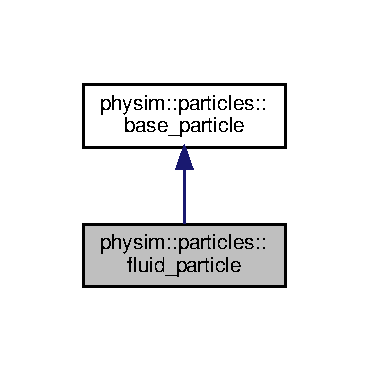
\includegraphics[width=177pt]{classphysim_1_1particles_1_1fluid__particle__inherit__graph}
\end{center}
\end{figure}


Collaboration diagram for physim\+:\+:particles\+:\+:fluid\+\_\+particle\+:\nopagebreak
\begin{figure}[H]
\begin{center}
\leavevmode
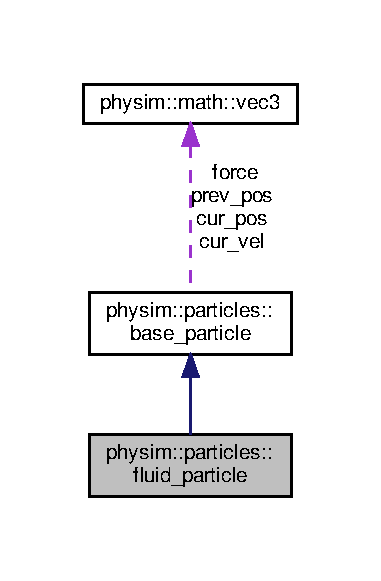
\includegraphics[width=183pt]{classphysim_1_1particles_1_1fluid__particle__coll__graph}
\end{center}
\end{figure}
\subsection*{Public Member Functions}
\begin{DoxyCompactItemize}
\item 
\mbox{\Hypertarget{classphysim_1_1particles_1_1fluid__particle_a0608e20564e48974f8d05ea1da1f5d8b}\label{classphysim_1_1particles_1_1fluid__particle_a0608e20564e48974f8d05ea1da1f5d8b}} 
\hyperlink{classphysim_1_1particles_1_1fluid__particle_a0608e20564e48974f8d05ea1da1f5d8b}{fluid\+\_\+particle} ()
\begin{DoxyCompactList}\small\item\em Default constructor. \end{DoxyCompactList}\item 
\mbox{\Hypertarget{classphysim_1_1particles_1_1fluid__particle_a1a60daa5bf72b641f46b7227e9b32a7e}\label{classphysim_1_1particles_1_1fluid__particle_a1a60daa5bf72b641f46b7227e9b32a7e}} 
\hyperlink{classphysim_1_1particles_1_1fluid__particle_a1a60daa5bf72b641f46b7227e9b32a7e}{fluid\+\_\+particle} (const \hyperlink{classphysim_1_1particles_1_1fluid__particle}{fluid\+\_\+particle} \&p)
\begin{DoxyCompactList}\small\item\em Copy constructor. \end{DoxyCompactList}\item 
\mbox{\Hypertarget{classphysim_1_1particles_1_1fluid__particle_afc95cf0e4346e59d54c222dae8c287f6}\label{classphysim_1_1particles_1_1fluid__particle_afc95cf0e4346e59d54c222dae8c287f6}} 
virtual \hyperlink{classphysim_1_1particles_1_1fluid__particle_afc95cf0e4346e59d54c222dae8c287f6}{$\sim$fluid\+\_\+particle} ()
\begin{DoxyCompactList}\small\item\em Destructor. \end{DoxyCompactList}\item 
virtual void \hyperlink{classphysim_1_1particles_1_1fluid__particle_a0aa522f9400bcb02373edd7bb073249b}{init} ()
\begin{DoxyCompactList}\small\item\em Initialises all particle\textquotesingle{}s attributes, most of them to null values. \end{DoxyCompactList}\item 
\mbox{\Hypertarget{classphysim_1_1particles_1_1fluid__particle_a14f4c27cc4268f98235b371e060ae996}\label{classphysim_1_1particles_1_1fluid__particle_a14f4c27cc4268f98235b371e060ae996}} 
virtual \hyperlink{namespacephysim_1_1particles_a068e6cda6626fbd381c07a9835425b08}{particle\+\_\+type} \hyperlink{classphysim_1_1particles_1_1fluid__particle_a14f4c27cc4268f98235b371e060ae996}{get\+\_\+particle\+\_\+type} () const
\begin{DoxyCompactList}\small\item\em Returns the type of this particle. \end{DoxyCompactList}\end{DoxyCompactItemize}
\subsection*{Public Attributes}
\begin{DoxyCompactItemize}
\item 
\mbox{\Hypertarget{classphysim_1_1particles_1_1fluid__particle_a0664c7d411aae32890f6fd359c74f2bc}\label{classphysim_1_1particles_1_1fluid__particle_a0664c7d411aae32890f6fd359c74f2bc}} 
float \hyperlink{classphysim_1_1particles_1_1fluid__particle_a0664c7d411aae32890f6fd359c74f2bc}{density}
\begin{DoxyCompactList}\small\item\em Density of the particle $\rho_i$. \mbox{[}Kg/m$^\wedge$3\mbox{]}. \end{DoxyCompactList}\item 
\mbox{\Hypertarget{classphysim_1_1particles_1_1fluid__particle_a2829dc6a83026e0854dd0ef4064f19b6}\label{classphysim_1_1particles_1_1fluid__particle_a2829dc6a83026e0854dd0ef4064f19b6}} 
float \hyperlink{classphysim_1_1particles_1_1fluid__particle_a2829dc6a83026e0854dd0ef4064f19b6}{pressure}
\begin{DoxyCompactList}\small\item\em Pressure of the particle $p_i$. \mbox{[}N/m$^\wedge$2\mbox{]}, \mbox{[}Kg/(m$\ast$s$^\wedge$2)\mbox{]}. \end{DoxyCompactList}\end{DoxyCompactItemize}
\subsection*{Private Member Functions}
\begin{DoxyCompactItemize}
\item 
void \hyperlink{classphysim_1_1particles_1_1fluid__particle_a5860aec6ef23bd4a700df26eb6b7b2f7}{partial\+\_\+init} ()
\begin{DoxyCompactList}\small\item\em Initialises this class\textquotesingle{}s attributes. \end{DoxyCompactList}\end{DoxyCompactItemize}


\subsection{Detailed Description}
Class implementing a fluid particle. 

A particle is a 0-\/dimensional object, subject to several forces. It can also collide with other objects in the scene (geometrical objects, see namespace \hyperlink{namespacephysim_1_1geometric}{physim\+::geometric}) but not with other particles. 

\subsection{Member Function Documentation}
\mbox{\Hypertarget{classphysim_1_1particles_1_1fluid__particle_a0aa522f9400bcb02373edd7bb073249b}\label{classphysim_1_1particles_1_1fluid__particle_a0aa522f9400bcb02373edd7bb073249b}} 
\index{physim\+::particles\+::fluid\+\_\+particle@{physim\+::particles\+::fluid\+\_\+particle}!init@{init}}
\index{init@{init}!physim\+::particles\+::fluid\+\_\+particle@{physim\+::particles\+::fluid\+\_\+particle}}
\subsubsection{\texorpdfstring{init()}{init()}}
{\footnotesize\ttfamily void physim\+::particles\+::fluid\+\_\+particle\+::init (\begin{DoxyParamCaption}{ }\end{DoxyParamCaption})\hspace{0.3cm}{\ttfamily [virtual]}}



Initialises all particle\textquotesingle{}s attributes, most of them to null values. 

The attributes of the class take the following values\+:
\begin{DoxyItemize}
\item \hyperlink{classphysim_1_1particles_1_1base__particle_a08072db6a1a59d21acc9cac6ac8965f7}{prev\+\_\+pos} \+: vec3(0,0,0)
\item \hyperlink{classphysim_1_1particles_1_1base__particle_a66a164d2a130c40901e3ec2709cdad43}{cur\+\_\+vel} \+: vec3(0,0,0)
\item \hyperlink{classphysim_1_1particles_1_1base__particle_adc3b11899d2e50970ae5d4931721a0ef}{force} \+: vec3(0,0,0)
\item \hyperlink{classphysim_1_1particles_1_1base__particle_acb5c9f0b4a911d8981210e2cfc4dda8a}{mass} \+: 1
\item \hyperlink{classphysim_1_1particles_1_1base__particle_a44f5de3bb4b860dfd511e28e1d6519d5}{index} \+: no value assigned, since it will be overwritten by the simulator. See \hyperlink{classphysim_1_1particles_1_1fluid__particle_a5860aec6ef23bd4a700df26eb6b7b2f7}{partial\+\_\+init()} to see how the attributes of this class are intialised. 
\end{DoxyItemize}

Reimplemented from \hyperlink{classphysim_1_1particles_1_1base__particle_a3bba517d51fd0bff7ec583e701765f87}{physim\+::particles\+::base\+\_\+particle}.

\mbox{\Hypertarget{classphysim_1_1particles_1_1fluid__particle_a5860aec6ef23bd4a700df26eb6b7b2f7}\label{classphysim_1_1particles_1_1fluid__particle_a5860aec6ef23bd4a700df26eb6b7b2f7}} 
\index{physim\+::particles\+::fluid\+\_\+particle@{physim\+::particles\+::fluid\+\_\+particle}!partial\+\_\+init@{partial\+\_\+init}}
\index{partial\+\_\+init@{partial\+\_\+init}!physim\+::particles\+::fluid\+\_\+particle@{physim\+::particles\+::fluid\+\_\+particle}}
\subsubsection{\texorpdfstring{partial\+\_\+init()}{partial\_init()}}
{\footnotesize\ttfamily void physim\+::particles\+::fluid\+\_\+particle\+::partial\+\_\+init (\begin{DoxyParamCaption}{ }\end{DoxyParamCaption})\hspace{0.3cm}{\ttfamily [private]}}



Initialises this class\textquotesingle{}s attributes. 

The attributes of the class take the following values\+:
\begin{DoxyItemize}
\item \hyperlink{classphysim_1_1particles_1_1fluid__particle_a0664c7d411aae32890f6fd359c74f2bc}{density} \+: 0.\+0
\item \hyperlink{classphysim_1_1particles_1_1fluid__particle_a2829dc6a83026e0854dd0ef4064f19b6}{pressure} \+: 0.\+0 
\end{DoxyItemize}

The documentation for this class was generated from the following files\+:\begin{DoxyCompactItemize}
\item 
physim/particles/fluid\+\_\+particle.\+hpp\item 
physim/particles/fluid\+\_\+particle.\+cpp\end{DoxyCompactItemize}

\hypertarget{classphysim_1_1emitters_1_1free__emitter}{}\section{physim\+:\+:emitters\+:\+:free\+\_\+emitter Class Reference}
\label{classphysim_1_1emitters_1_1free__emitter}\index{physim\+::emitters\+::free\+\_\+emitter@{physim\+::emitters\+::free\+\_\+emitter}}


Class for free particle initialisation.  




{\ttfamily \#include $<$free\+\_\+emitter.\+hpp$>$}



Inheritance diagram for physim\+:\+:emitters\+:\+:free\+\_\+emitter\+:\nopagebreak
\begin{figure}[H]
\begin{center}
\leavevmode
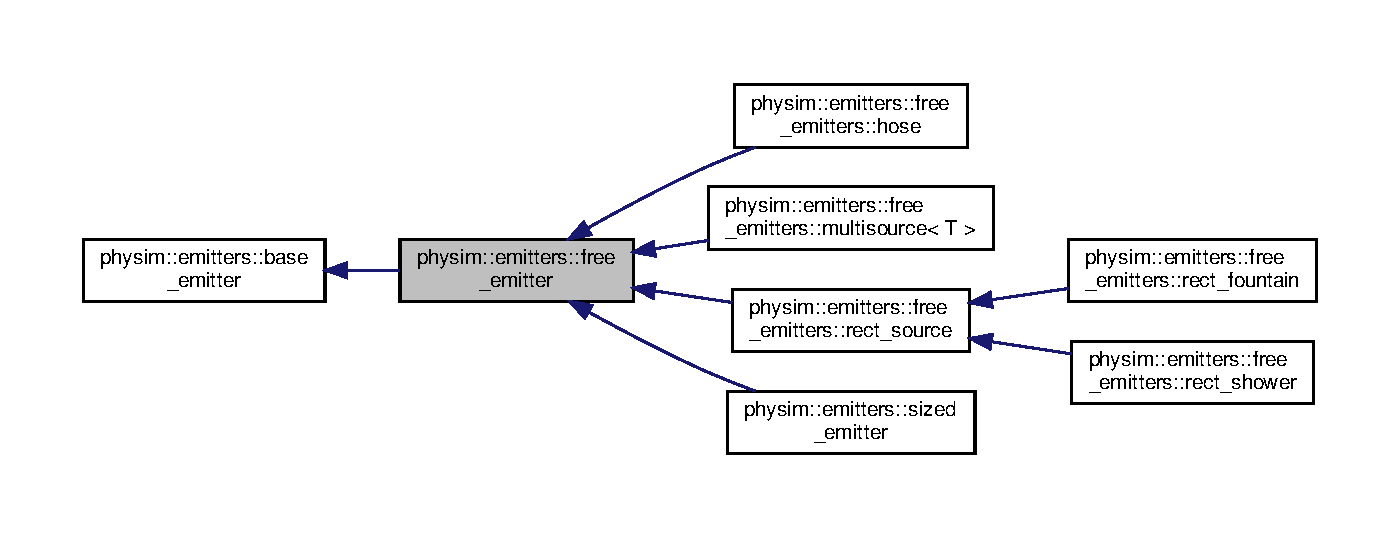
\includegraphics[width=350pt]{classphysim_1_1emitters_1_1free__emitter__inherit__graph}
\end{center}
\end{figure}


Collaboration diagram for physim\+:\+:emitters\+:\+:free\+\_\+emitter\+:\nopagebreak
\begin{figure}[H]
\begin{center}
\leavevmode
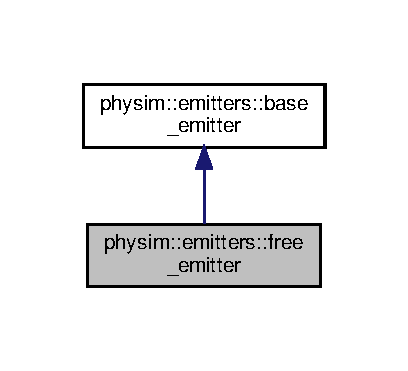
\includegraphics[width=196pt]{classphysim_1_1emitters_1_1free__emitter__coll__graph}
\end{center}
\end{figure}
\subsection*{Public Member Functions}
\begin{DoxyCompactItemize}
\item 
\mbox{\Hypertarget{classphysim_1_1emitters_1_1free__emitter_a510e60d9de5438fc91494b5018329bc1}\label{classphysim_1_1emitters_1_1free__emitter_a510e60d9de5438fc91494b5018329bc1}} 
\hyperlink{classphysim_1_1emitters_1_1free__emitter_a510e60d9de5438fc91494b5018329bc1}{free\+\_\+emitter} ()
\begin{DoxyCompactList}\small\item\em Default constructor. \end{DoxyCompactList}\item 
\mbox{\Hypertarget{classphysim_1_1emitters_1_1free__emitter_a2a9ae9952f735c67c0138c3385bf59a4}\label{classphysim_1_1emitters_1_1free__emitter_a2a9ae9952f735c67c0138c3385bf59a4}} 
\hyperlink{classphysim_1_1emitters_1_1free__emitter_a2a9ae9952f735c67c0138c3385bf59a4}{free\+\_\+emitter} (const \hyperlink{classphysim_1_1emitters_1_1free__emitter}{free\+\_\+emitter} \&i)
\begin{DoxyCompactList}\small\item\em Copy constructor. \end{DoxyCompactList}\item 
\mbox{\Hypertarget{classphysim_1_1emitters_1_1free__emitter_ae9777b2e847f64d0e3a88a6b96979c9d}\label{classphysim_1_1emitters_1_1free__emitter_ae9777b2e847f64d0e3a88a6b96979c9d}} 
virtual \hyperlink{classphysim_1_1emitters_1_1free__emitter_ae9777b2e847f64d0e3a88a6b96979c9d}{$\sim$free\+\_\+emitter} ()
\begin{DoxyCompactList}\small\item\em Destructor. \end{DoxyCompactList}\item 
\mbox{\Hypertarget{classphysim_1_1emitters_1_1free__emitter_a72d9b7819fceb26e5b0d087977ed17b4}\label{classphysim_1_1emitters_1_1free__emitter_a72d9b7819fceb26e5b0d087977ed17b4}} 
void \hyperlink{classphysim_1_1emitters_1_1free__emitter_a72d9b7819fceb26e5b0d087977ed17b4}{set\+\_\+charge\+\_\+initialiser} (const \hyperlink{namespacephysim_1_1emitters_a68725a630c2e0c1b4cdff4ca0ee174ac}{free\+\_\+emit} \&f)
\begin{DoxyCompactList}\small\item\em Sets the charge initialiser. See \hyperlink{classphysim_1_1emitters_1_1free__emitter_a895244d2023c4cc72658d356bdb51b9a}{charge}. \end{DoxyCompactList}\item 
\mbox{\Hypertarget{classphysim_1_1emitters_1_1free__emitter_af4637cf82df4505e3c301756f3706c6f}\label{classphysim_1_1emitters_1_1free__emitter_af4637cf82df4505e3c301756f3706c6f}} 
void \hyperlink{classphysim_1_1emitters_1_1free__emitter_af4637cf82df4505e3c301756f3706c6f}{set\+\_\+bounce\+\_\+initialiser} (const \hyperlink{namespacephysim_1_1emitters_a68725a630c2e0c1b4cdff4ca0ee174ac}{free\+\_\+emit} \&f)
\begin{DoxyCompactList}\small\item\em Sets the bouncing coefficient initialiser. See \hyperlink{classphysim_1_1emitters_1_1free__emitter_a71006743e284b12904d7a4b4127ab4b8}{bounce}. \end{DoxyCompactList}\item 
\mbox{\Hypertarget{classphysim_1_1emitters_1_1free__emitter_aa88ce38ef6ac282aabf50f93d7eefffe}\label{classphysim_1_1emitters_1_1free__emitter_aa88ce38ef6ac282aabf50f93d7eefffe}} 
void \hyperlink{classphysim_1_1emitters_1_1free__emitter_aa88ce38ef6ac282aabf50f93d7eefffe}{set\+\_\+friction\+\_\+initialiser} (const \hyperlink{namespacephysim_1_1emitters_a68725a630c2e0c1b4cdff4ca0ee174ac}{free\+\_\+emit} \&f)
\begin{DoxyCompactList}\small\item\em Sets the friction coefficient initialiser. See \hyperlink{classphysim_1_1emitters_1_1free__emitter_a0167889dfac9483e7e2690efc353a7bd}{friction}. \end{DoxyCompactList}\item 
\mbox{\Hypertarget{classphysim_1_1emitters_1_1free__emitter_a7921765ed3be2162a2710a9ea74cfa30}\label{classphysim_1_1emitters_1_1free__emitter_a7921765ed3be2162a2710a9ea74cfa30}} 
void \hyperlink{classphysim_1_1emitters_1_1free__emitter_a7921765ed3be2162a2710a9ea74cfa30}{set\+\_\+lifetime\+\_\+initialiser} (const \hyperlink{namespacephysim_1_1emitters_a68725a630c2e0c1b4cdff4ca0ee174ac}{free\+\_\+emit} \&f)
\begin{DoxyCompactList}\small\item\em Sets the lifetime initialiser. See \hyperlink{classphysim_1_1emitters_1_1free__emitter_a596108fe3602299fa9035ece668653d4}{lifetime}. \end{DoxyCompactList}\item 
\mbox{\Hypertarget{classphysim_1_1emitters_1_1free__emitter_a4a8e6ec80cce24bf39477af6cc6664c9}\label{classphysim_1_1emitters_1_1free__emitter_a4a8e6ec80cce24bf39477af6cc6664c9}} 
void \hyperlink{classphysim_1_1emitters_1_1free__emitter_a4a8e6ec80cce24bf39477af6cc6664c9}{set\+\_\+starttime\+\_\+initialiser} (const \hyperlink{namespacephysim_1_1emitters_a68725a630c2e0c1b4cdff4ca0ee174ac}{free\+\_\+emit} \&f)
\begin{DoxyCompactList}\small\item\em Sets the starttime initialiser. See \hyperlink{classphysim_1_1emitters_1_1free__emitter_af296f735438087c4acaba2242c839e49}{starttime}. \end{DoxyCompactList}\item 
\mbox{\Hypertarget{classphysim_1_1emitters_1_1free__emitter_ac07a83dbd4863d0c121828fa95389572}\label{classphysim_1_1emitters_1_1free__emitter_ac07a83dbd4863d0c121828fa95389572}} 
void \hyperlink{classphysim_1_1emitters_1_1free__emitter_ac07a83dbd4863d0c121828fa95389572}{set\+\_\+fixed\+\_\+initialiser} (const \hyperlink{namespacephysim_1_1emitters_a68725a630c2e0c1b4cdff4ca0ee174ac}{free\+\_\+emit} \&f)
\begin{DoxyCompactList}\small\item\em Sets the fixed initialiser. See \hyperlink{classphysim_1_1emitters_1_1free__emitter_a2561dbe073b699e28fbb7ad10e897567}{fixed}. \end{DoxyCompactList}\item 
\mbox{\Hypertarget{classphysim_1_1emitters_1_1free__emitter_a7b731506d65270400b197428a63f2eb1}\label{classphysim_1_1emitters_1_1free__emitter_a7b731506d65270400b197428a63f2eb1}} 
virtual \hyperlink{classphysim_1_1emitters_1_1free__emitter}{free\+\_\+emitter} $\ast$ \hyperlink{classphysim_1_1emitters_1_1free__emitter_a7b731506d65270400b197428a63f2eb1}{clone} () const
\begin{DoxyCompactList}\small\item\em Returns a reference to a copy of this emitter. \end{DoxyCompactList}\item 
\mbox{\Hypertarget{classphysim_1_1emitters_1_1free__emitter_af4469672062a3f1ec6493b9b8de9e7c9}\label{classphysim_1_1emitters_1_1free__emitter_af4469672062a3f1ec6493b9b8de9e7c9}} 
const \hyperlink{namespacephysim_1_1emitters_a68725a630c2e0c1b4cdff4ca0ee174ac}{free\+\_\+emit} \& \hyperlink{classphysim_1_1emitters_1_1free__emitter_af4469672062a3f1ec6493b9b8de9e7c9}{get\+\_\+charge\+\_\+initialiser} () const
\begin{DoxyCompactList}\small\item\em Returns the charge initialiser. See \hyperlink{classphysim_1_1emitters_1_1free__emitter_a895244d2023c4cc72658d356bdb51b9a}{charge}. \end{DoxyCompactList}\item 
\mbox{\Hypertarget{classphysim_1_1emitters_1_1free__emitter_a4f0900702881c524ac89f7b41f662b82}\label{classphysim_1_1emitters_1_1free__emitter_a4f0900702881c524ac89f7b41f662b82}} 
const \hyperlink{namespacephysim_1_1emitters_a68725a630c2e0c1b4cdff4ca0ee174ac}{free\+\_\+emit} \& \hyperlink{classphysim_1_1emitters_1_1free__emitter_a4f0900702881c524ac89f7b41f662b82}{get\+\_\+bounce\+\_\+initialiser} () const
\begin{DoxyCompactList}\small\item\em Returns the bouncing coefficient initialiser. See \hyperlink{classphysim_1_1emitters_1_1free__emitter_a71006743e284b12904d7a4b4127ab4b8}{bounce}. \end{DoxyCompactList}\item 
\mbox{\Hypertarget{classphysim_1_1emitters_1_1free__emitter_a6e7acea19f9f26fbf36b032780ea0b43}\label{classphysim_1_1emitters_1_1free__emitter_a6e7acea19f9f26fbf36b032780ea0b43}} 
const \hyperlink{namespacephysim_1_1emitters_a68725a630c2e0c1b4cdff4ca0ee174ac}{free\+\_\+emit} \& \hyperlink{classphysim_1_1emitters_1_1free__emitter_a6e7acea19f9f26fbf36b032780ea0b43}{get\+\_\+friction\+\_\+initialiser} () const
\begin{DoxyCompactList}\small\item\em Returns the friction coefficient initialiser. See \hyperlink{classphysim_1_1emitters_1_1free__emitter_a0167889dfac9483e7e2690efc353a7bd}{friction}. \end{DoxyCompactList}\item 
\mbox{\Hypertarget{classphysim_1_1emitters_1_1free__emitter_ac99b79f8208ab9bc0d6cc86e2d19146e}\label{classphysim_1_1emitters_1_1free__emitter_ac99b79f8208ab9bc0d6cc86e2d19146e}} 
const \hyperlink{namespacephysim_1_1emitters_a68725a630c2e0c1b4cdff4ca0ee174ac}{free\+\_\+emit} \& \hyperlink{classphysim_1_1emitters_1_1free__emitter_ac99b79f8208ab9bc0d6cc86e2d19146e}{get\+\_\+lifetime\+\_\+initialiser} () const
\begin{DoxyCompactList}\small\item\em Returns the lifetime initialiser. See \hyperlink{classphysim_1_1emitters_1_1free__emitter_a596108fe3602299fa9035ece668653d4}{lifetime}. \end{DoxyCompactList}\item 
\mbox{\Hypertarget{classphysim_1_1emitters_1_1free__emitter_a2236e9631ecbbd4cdb081cf16c91ced0}\label{classphysim_1_1emitters_1_1free__emitter_a2236e9631ecbbd4cdb081cf16c91ced0}} 
const \hyperlink{namespacephysim_1_1emitters_a68725a630c2e0c1b4cdff4ca0ee174ac}{free\+\_\+emit} \& \hyperlink{classphysim_1_1emitters_1_1free__emitter_a2236e9631ecbbd4cdb081cf16c91ced0}{get\+\_\+starttime\+\_\+initialiser} () const
\begin{DoxyCompactList}\small\item\em Returns the starttime initialiser. See \hyperlink{classphysim_1_1emitters_1_1free__emitter_af296f735438087c4acaba2242c839e49}{starttime}. \end{DoxyCompactList}\item 
\mbox{\Hypertarget{classphysim_1_1emitters_1_1free__emitter_a1edff9931b38d73b24e4b326e998be20}\label{classphysim_1_1emitters_1_1free__emitter_a1edff9931b38d73b24e4b326e998be20}} 
const \hyperlink{namespacephysim_1_1emitters_a68725a630c2e0c1b4cdff4ca0ee174ac}{free\+\_\+emit} \& \hyperlink{classphysim_1_1emitters_1_1free__emitter_a1edff9931b38d73b24e4b326e998be20}{get\+\_\+fixed\+\_\+initialiser} () const
\begin{DoxyCompactList}\small\item\em Returns the fixed initialiser. See \hyperlink{classphysim_1_1emitters_1_1free__emitter_a2561dbe073b699e28fbb7ad10e897567}{fixed}. \end{DoxyCompactList}\item 
void \hyperlink{classphysim_1_1emitters_1_1free__emitter_a6cdf0656c3951792b902cfbafd5ed79d}{initialise\+\_\+particle} (\hyperlink{classphysim_1_1particles_1_1free__particle}{particles\+::free\+\_\+particle} \&p) const
\begin{DoxyCompactList}\small\item\em Initialise a particle. \end{DoxyCompactList}\end{DoxyCompactItemize}
\subsection*{Protected Attributes}
\begin{DoxyCompactItemize}
\item 
\mbox{\Hypertarget{classphysim_1_1emitters_1_1free__emitter_a895244d2023c4cc72658d356bdb51b9a}\label{classphysim_1_1emitters_1_1free__emitter_a895244d2023c4cc72658d356bdb51b9a}} 
\hyperlink{namespacephysim_1_1emitters_a68725a630c2e0c1b4cdff4ca0ee174ac}{free\+\_\+emit} \hyperlink{classphysim_1_1emitters_1_1free__emitter_a895244d2023c4cc72658d356bdb51b9a}{charge}
\begin{DoxyCompactList}\small\item\em Initialiser of the charge. \end{DoxyCompactList}\item 
\mbox{\Hypertarget{classphysim_1_1emitters_1_1free__emitter_a0167889dfac9483e7e2690efc353a7bd}\label{classphysim_1_1emitters_1_1free__emitter_a0167889dfac9483e7e2690efc353a7bd}} 
\hyperlink{namespacephysim_1_1emitters_a68725a630c2e0c1b4cdff4ca0ee174ac}{free\+\_\+emit} \hyperlink{classphysim_1_1emitters_1_1free__emitter_a0167889dfac9483e7e2690efc353a7bd}{friction}
\begin{DoxyCompactList}\small\item\em Initialiser of the friction coefficient. \end{DoxyCompactList}\item 
\mbox{\Hypertarget{classphysim_1_1emitters_1_1free__emitter_a71006743e284b12904d7a4b4127ab4b8}\label{classphysim_1_1emitters_1_1free__emitter_a71006743e284b12904d7a4b4127ab4b8}} 
\hyperlink{namespacephysim_1_1emitters_a68725a630c2e0c1b4cdff4ca0ee174ac}{free\+\_\+emit} \hyperlink{classphysim_1_1emitters_1_1free__emitter_a71006743e284b12904d7a4b4127ab4b8}{bounce}
\begin{DoxyCompactList}\small\item\em Initialiser of the bouncing coefficient. \end{DoxyCompactList}\item 
\mbox{\Hypertarget{classphysim_1_1emitters_1_1free__emitter_a596108fe3602299fa9035ece668653d4}\label{classphysim_1_1emitters_1_1free__emitter_a596108fe3602299fa9035ece668653d4}} 
\hyperlink{namespacephysim_1_1emitters_a68725a630c2e0c1b4cdff4ca0ee174ac}{free\+\_\+emit} \hyperlink{classphysim_1_1emitters_1_1free__emitter_a596108fe3602299fa9035ece668653d4}{lifetime}
\begin{DoxyCompactList}\small\item\em Initialiser of the lifetime. \end{DoxyCompactList}\item 
\mbox{\Hypertarget{classphysim_1_1emitters_1_1free__emitter_af296f735438087c4acaba2242c839e49}\label{classphysim_1_1emitters_1_1free__emitter_af296f735438087c4acaba2242c839e49}} 
\hyperlink{namespacephysim_1_1emitters_a68725a630c2e0c1b4cdff4ca0ee174ac}{free\+\_\+emit} \hyperlink{classphysim_1_1emitters_1_1free__emitter_af296f735438087c4acaba2242c839e49}{starttime}
\begin{DoxyCompactList}\small\item\em Initialiser of the starttime. \end{DoxyCompactList}\item 
\mbox{\Hypertarget{classphysim_1_1emitters_1_1free__emitter_a2561dbe073b699e28fbb7ad10e897567}\label{classphysim_1_1emitters_1_1free__emitter_a2561dbe073b699e28fbb7ad10e897567}} 
\hyperlink{namespacephysim_1_1emitters_a68725a630c2e0c1b4cdff4ca0ee174ac}{free\+\_\+emit} \hyperlink{classphysim_1_1emitters_1_1free__emitter_a2561dbe073b699e28fbb7ad10e897567}{fixed}
\begin{DoxyCompactList}\small\item\em Initialiser of the \textquotesingle{}fixed\textquotesingle{} attribute. \end{DoxyCompactList}\end{DoxyCompactItemize}


\subsection{Detailed Description}
Class for free particle initialisation. 

This class is used to initialise the attributes of a free particle.

This class has several functions as attributes, each of which initialises an attribute of the particle.

These functions are\+:
\begin{DoxyItemize}
\item \hyperlink{classphysim_1_1emitters_1_1base__emitter_ac67584a2ca34232c1f4f04c41599df0e}{pos} \+: function used to initialise the position of a particle.
\item \hyperlink{classphysim_1_1emitters_1_1base__emitter_a9ea19d96450cff65882371b61a2294c8}{vel} \+: function used to initialise the velocity of a particle.
\item \hyperlink{classphysim_1_1emitters_1_1base__emitter_a4e1b65730afef86899544d3306f7547d}{mass} \+: function to initialise the mass of the particle.
\item \hyperlink{classphysim_1_1emitters_1_1free__emitter_a895244d2023c4cc72658d356bdb51b9a}{charge} \+: function used to initialise the charge of a particle.
\item \hyperlink{classphysim_1_1emitters_1_1free__emitter_a0167889dfac9483e7e2690efc353a7bd}{friction} \+: function used to initialise the friction coefficient of a particle.
\item \hyperlink{classphysim_1_1emitters_1_1free__emitter_a71006743e284b12904d7a4b4127ab4b8}{bounce} \+: function used to initialise the bouncing coefficient of a particle.
\item \hyperlink{classphysim_1_1emitters_1_1free__emitter_a596108fe3602299fa9035ece668653d4}{lifetime} \+: function used to initialise the lifetime of a particle.
\item \hyperlink{classphysim_1_1emitters_1_1free__emitter_af296f735438087c4acaba2242c839e49}{starttime} \+: function used to initialise the starting time of a particle.
\item \hyperlink{classphysim_1_1emitters_1_1free__emitter_a2561dbe073b699e28fbb7ad10e897567}{fixed} \+: function used to initialise the fixed attribute of a particle. this function is used to initialse the radius attribute of the particle).
\end{DoxyItemize}

By default, all these function\textquotesingle{}s behaviour is to initialise a particle the same way they are initialised when constructed (see \hyperlink{classphysim_1_1particles_1_1free__particle_a0df21e64a28c5fdf471d54a50b59fea3}{free\+\_\+particle\+::init}).

Also, they are applied in the same order as they appear listed. Therefore, for example, the position attributes can be used to initialise the velocity. Finally, it is guaranteed that all these functions will be called after the \hyperlink{classphysim_1_1simulator}{simulator} has assigned an index to the particle being initialised.

The previous position of a particle is updated automatically after initialising all attributes using the functions, but on the simulator. Therefore, there is no need to initialise it.

The initialisation of the particle takes place in the method \hyperlink{classphysim_1_1emitters_1_1free__emitter_a6cdf0656c3951792b902cfbafd5ed79d}{initialise\+\_\+particle(free\+\_\+particle\&)const}.

Finally, all classes must implement the \hyperlink{classphysim_1_1emitters_1_1free__emitter_a7b731506d65270400b197428a63f2eb1}{clone} function. 

\subsection{Member Function Documentation}
\mbox{\Hypertarget{classphysim_1_1emitters_1_1free__emitter_a6cdf0656c3951792b902cfbafd5ed79d}\label{classphysim_1_1emitters_1_1free__emitter_a6cdf0656c3951792b902cfbafd5ed79d}} 
\index{physim\+::emitters\+::free\+\_\+emitter@{physim\+::emitters\+::free\+\_\+emitter}!initialise\+\_\+particle@{initialise\+\_\+particle}}
\index{initialise\+\_\+particle@{initialise\+\_\+particle}!physim\+::emitters\+::free\+\_\+emitter@{physim\+::emitters\+::free\+\_\+emitter}}
\subsubsection{\texorpdfstring{initialise\+\_\+particle()}{initialise\_particle()}}
{\footnotesize\ttfamily void physim\+::emitters\+::free\+\_\+emitter\+::initialise\+\_\+particle (\begin{DoxyParamCaption}\item[{\hyperlink{classphysim_1_1particles_1_1free__particle}{particles\+::free\+\_\+particle} \&}]{p }\end{DoxyParamCaption}) const}



Initialise a particle. 

Each of the functions for particle initialisation are called on the particle. For details on the order, see the description of this class. 
\begin{DoxyParams}{Parameters}
{\em p} & The particle to be initialised. \\
\hline
\end{DoxyParams}


The documentation for this class was generated from the following files\+:\begin{DoxyCompactItemize}
\item 
physim/emitter/free\+\_\+emitter.\+hpp\item 
physim/emitter/free\+\_\+emitter.\+cpp\end{DoxyCompactItemize}

\hypertarget{classphysim_1_1particles_1_1free__particle}{}\section{physim\+:\+:particles\+:\+:free\+\_\+particle Class Reference}
\label{classphysim_1_1particles_1_1free__particle}\index{physim\+::particles\+::free\+\_\+particle@{physim\+::particles\+::free\+\_\+particle}}


Class implementing a free particle.  




{\ttfamily \#include $<$free\+\_\+particle.\+hpp$>$}



Inheritance diagram for physim\+:\+:particles\+:\+:free\+\_\+particle\+:\nopagebreak
\begin{figure}[H]
\begin{center}
\leavevmode
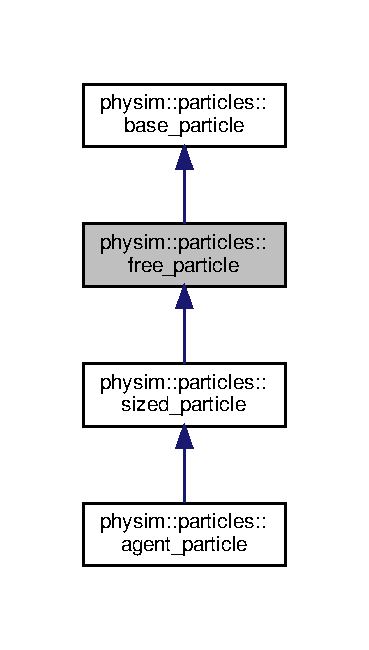
\includegraphics[width=177pt]{classphysim_1_1particles_1_1free__particle__inherit__graph}
\end{center}
\end{figure}


Collaboration diagram for physim\+:\+:particles\+:\+:free\+\_\+particle\+:\nopagebreak
\begin{figure}[H]
\begin{center}
\leavevmode
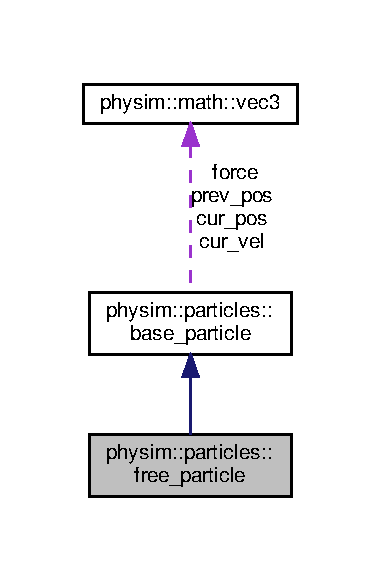
\includegraphics[width=183pt]{classphysim_1_1particles_1_1free__particle__coll__graph}
\end{center}
\end{figure}
\subsection*{Public Member Functions}
\begin{DoxyCompactItemize}
\item 
\mbox{\Hypertarget{classphysim_1_1particles_1_1free__particle_a49daf863274486e00c8adce24d78e3bb}\label{classphysim_1_1particles_1_1free__particle_a49daf863274486e00c8adce24d78e3bb}} 
\hyperlink{classphysim_1_1particles_1_1free__particle_a49daf863274486e00c8adce24d78e3bb}{free\+\_\+particle} ()
\begin{DoxyCompactList}\small\item\em Default constructor. \end{DoxyCompactList}\item 
\mbox{\Hypertarget{classphysim_1_1particles_1_1free__particle_aa075ca6679e0f74cacaba04a3457e782}\label{classphysim_1_1particles_1_1free__particle_aa075ca6679e0f74cacaba04a3457e782}} 
\hyperlink{classphysim_1_1particles_1_1free__particle_aa075ca6679e0f74cacaba04a3457e782}{free\+\_\+particle} (const \hyperlink{classphysim_1_1particles_1_1free__particle}{free\+\_\+particle} \&p)
\begin{DoxyCompactList}\small\item\em Copy constructor. \end{DoxyCompactList}\item 
\mbox{\Hypertarget{classphysim_1_1particles_1_1free__particle_a14b490652a1ca90950382c86f55e510a}\label{classphysim_1_1particles_1_1free__particle_a14b490652a1ca90950382c86f55e510a}} 
virtual \hyperlink{classphysim_1_1particles_1_1free__particle_a14b490652a1ca90950382c86f55e510a}{$\sim$free\+\_\+particle} ()
\begin{DoxyCompactList}\small\item\em Destructor. \end{DoxyCompactList}\item 
void \hyperlink{classphysim_1_1particles_1_1free__particle_a8b8e76a24759a1e0a5d3b0d4933e31c1}{reduce\+\_\+lifetime} (float t)
\begin{DoxyCompactList}\small\item\em Decreases the lifetime by {\itshape t}. \end{DoxyCompactList}\item 
void \hyperlink{classphysim_1_1particles_1_1free__particle_a8f024371fb279e75bbfef1be83bce4bc}{reduce\+\_\+starttime} (float t)
\begin{DoxyCompactList}\small\item\em Decreases the starttime by {\itshape t}. \end{DoxyCompactList}\item 
virtual void \hyperlink{classphysim_1_1particles_1_1free__particle_a0df21e64a28c5fdf471d54a50b59fea3}{init} ()
\begin{DoxyCompactList}\small\item\em Initialises all particle\textquotesingle{}s attributes, most of them to null values. \end{DoxyCompactList}\item 
\mbox{\Hypertarget{classphysim_1_1particles_1_1free__particle_a3400dd6813c8501646d10ca592f0d67d}\label{classphysim_1_1particles_1_1free__particle_a3400dd6813c8501646d10ca592f0d67d}} 
virtual \hyperlink{namespacephysim_1_1particles_a068e6cda6626fbd381c07a9835425b08}{particle\+\_\+type} \hyperlink{classphysim_1_1particles_1_1free__particle_a3400dd6813c8501646d10ca592f0d67d}{get\+\_\+particle\+\_\+type} () const
\begin{DoxyCompactList}\small\item\em Returns the type of this particle. \end{DoxyCompactList}\end{DoxyCompactItemize}
\subsection*{Public Attributes}
\begin{DoxyCompactItemize}
\item 
\mbox{\Hypertarget{classphysim_1_1particles_1_1free__particle_aac766fa5294e47b944d32ca3e38d47fa}\label{classphysim_1_1particles_1_1free__particle_aac766fa5294e47b944d32ca3e38d47fa}} 
float \hyperlink{classphysim_1_1particles_1_1free__particle_aac766fa5294e47b944d32ca3e38d47fa}{bouncing}
\begin{DoxyCompactList}\small\item\em Bouncing coefficient of the particle. \end{DoxyCompactList}\item 
\mbox{\Hypertarget{classphysim_1_1particles_1_1free__particle_a9e7dfd81e9392fc42b3faecb57afdc02}\label{classphysim_1_1particles_1_1free__particle_a9e7dfd81e9392fc42b3faecb57afdc02}} 
float \hyperlink{classphysim_1_1particles_1_1free__particle_a9e7dfd81e9392fc42b3faecb57afdc02}{friction}
\begin{DoxyCompactList}\small\item\em Friction coefficient of the particle. \end{DoxyCompactList}\item 
\mbox{\Hypertarget{classphysim_1_1particles_1_1free__particle_a7513ac41f3cab1ce083f8695e2c73301}\label{classphysim_1_1particles_1_1free__particle_a7513ac41f3cab1ce083f8695e2c73301}} 
float \hyperlink{classphysim_1_1particles_1_1free__particle_a7513ac41f3cab1ce083f8695e2c73301}{charge}
\begin{DoxyCompactList}\small\item\em Electrical charge of the particle \mbox{[}C\mbox{]}. \end{DoxyCompactList}\item 
float \hyperlink{classphysim_1_1particles_1_1free__particle_a5870d6fd3167d2c6120f887f45fe50fc}{lifetime}
\begin{DoxyCompactList}\small\item\em Lifetime of the particle \mbox{[}s\mbox{]}. \end{DoxyCompactList}\item 
float \hyperlink{classphysim_1_1particles_1_1free__particle_ad0379ba926ecc909bfbfb373045bfcf9}{starttime}
\begin{DoxyCompactList}\small\item\em Starting time of a particle \mbox{[}s\mbox{]}. \end{DoxyCompactList}\item 
bool \hyperlink{classphysim_1_1particles_1_1free__particle_a0f6d69caeac140abd74c7be4ed55eb74}{fixed}
\begin{DoxyCompactList}\small\item\em Is this particle fixed? \end{DoxyCompactList}\end{DoxyCompactItemize}
\subsection*{Private Member Functions}
\begin{DoxyCompactItemize}
\item 
void \hyperlink{classphysim_1_1particles_1_1free__particle_a967f3229ac014999de8f9823882c60e8}{partial\+\_\+init} ()
\begin{DoxyCompactList}\small\item\em Initialises this class\textquotesingle{}s attributes. \end{DoxyCompactList}\end{DoxyCompactItemize}


\subsection{Detailed Description}
Class implementing a free particle. 

A free particle is a 0-\/dimensional object, subject to several forces but not to any other particle\textquotesingle{}s direct interaction through them. It can collide with other objects in the scene (geometrical objects, see namespace \hyperlink{namespacephysim_1_1geometric}{physim\+::geometric}) but not with other particles.

All this class\textquotesingle{} attributes are public. 

\subsection{Member Function Documentation}
\mbox{\Hypertarget{classphysim_1_1particles_1_1free__particle_a0df21e64a28c5fdf471d54a50b59fea3}\label{classphysim_1_1particles_1_1free__particle_a0df21e64a28c5fdf471d54a50b59fea3}} 
\index{physim\+::particles\+::free\+\_\+particle@{physim\+::particles\+::free\+\_\+particle}!init@{init}}
\index{init@{init}!physim\+::particles\+::free\+\_\+particle@{physim\+::particles\+::free\+\_\+particle}}
\subsubsection{\texorpdfstring{init()}{init()}}
{\footnotesize\ttfamily void physim\+::particles\+::free\+\_\+particle\+::init (\begin{DoxyParamCaption}{ }\end{DoxyParamCaption})\hspace{0.3cm}{\ttfamily [virtual]}}



Initialises all particle\textquotesingle{}s attributes, most of them to null values. 

The attributes of the class take the following values\+:
\begin{DoxyItemize}
\item \hyperlink{classphysim_1_1particles_1_1base__particle_a08072db6a1a59d21acc9cac6ac8965f7}{prev\+\_\+pos} \+: vec3(0,0,0)
\item \hyperlink{classphysim_1_1particles_1_1base__particle_a66a164d2a130c40901e3ec2709cdad43}{cur\+\_\+vel} \+: vec3(0,0,0)
\item \hyperlink{classphysim_1_1particles_1_1base__particle_adc3b11899d2e50970ae5d4931721a0ef}{force} \+: vec3(0,0,0)
\item \hyperlink{classphysim_1_1particles_1_1base__particle_acb5c9f0b4a911d8981210e2cfc4dda8a}{mass} \+: 1
\item \hyperlink{classphysim_1_1particles_1_1base__particle_a44f5de3bb4b860dfd511e28e1d6519d5}{index} \+: no value assigned, since it will be overwritten by the simulator. See \hyperlink{classphysim_1_1particles_1_1free__particle_a967f3229ac014999de8f9823882c60e8}{partial\+\_\+init()} to see how the attributes of this class are intialised. 
\end{DoxyItemize}

Reimplemented from \hyperlink{classphysim_1_1particles_1_1base__particle_a3bba517d51fd0bff7ec583e701765f87}{physim\+::particles\+::base\+\_\+particle}.



Reimplemented in \hyperlink{classphysim_1_1particles_1_1agent__particle_ac13082909f480fc55d406321c77d38b1}{physim\+::particles\+::agent\+\_\+particle}, and \hyperlink{classphysim_1_1particles_1_1sized__particle_a63de84961417c1522c0ca576697cd972}{physim\+::particles\+::sized\+\_\+particle}.

\mbox{\Hypertarget{classphysim_1_1particles_1_1free__particle_a967f3229ac014999de8f9823882c60e8}\label{classphysim_1_1particles_1_1free__particle_a967f3229ac014999de8f9823882c60e8}} 
\index{physim\+::particles\+::free\+\_\+particle@{physim\+::particles\+::free\+\_\+particle}!partial\+\_\+init@{partial\+\_\+init}}
\index{partial\+\_\+init@{partial\+\_\+init}!physim\+::particles\+::free\+\_\+particle@{physim\+::particles\+::free\+\_\+particle}}
\subsubsection{\texorpdfstring{partial\+\_\+init()}{partial\_init()}}
{\footnotesize\ttfamily void physim\+::particles\+::free\+\_\+particle\+::partial\+\_\+init (\begin{DoxyParamCaption}{ }\end{DoxyParamCaption})\hspace{0.3cm}{\ttfamily [private]}}



Initialises this class\textquotesingle{}s attributes. 

The attributes of the class take the following values\+:
\begin{DoxyItemize}
\item \hyperlink{classphysim_1_1particles_1_1free__particle_aac766fa5294e47b944d32ca3e38d47fa}{bouncing} \+: 0.\+8
\item \hyperlink{classphysim_1_1particles_1_1free__particle_a9e7dfd81e9392fc42b3faecb57afdc02}{friction} \+: 0.\+2
\item \hyperlink{classphysim_1_1particles_1_1free__particle_a7513ac41f3cab1ce083f8695e2c73301}{charge} \+: 0
\item \hyperlink{classphysim_1_1particles_1_1free__particle_a5870d6fd3167d2c6120f887f45fe50fc}{lifetime} \+: 10
\item \hyperlink{classphysim_1_1particles_1_1free__particle_ad0379ba926ecc909bfbfb373045bfcf9}{starttime} \+: 0
\item \hyperlink{classphysim_1_1particles_1_1free__particle_a0f6d69caeac140abd74c7be4ed55eb74}{fixed} \+: false 
\end{DoxyItemize}\mbox{\Hypertarget{classphysim_1_1particles_1_1free__particle_a8b8e76a24759a1e0a5d3b0d4933e31c1}\label{classphysim_1_1particles_1_1free__particle_a8b8e76a24759a1e0a5d3b0d4933e31c1}} 
\index{physim\+::particles\+::free\+\_\+particle@{physim\+::particles\+::free\+\_\+particle}!reduce\+\_\+lifetime@{reduce\+\_\+lifetime}}
\index{reduce\+\_\+lifetime@{reduce\+\_\+lifetime}!physim\+::particles\+::free\+\_\+particle@{physim\+::particles\+::free\+\_\+particle}}
\subsubsection{\texorpdfstring{reduce\+\_\+lifetime()}{reduce\_lifetime()}}
{\footnotesize\ttfamily void physim\+::particles\+::free\+\_\+particle\+::reduce\+\_\+lifetime (\begin{DoxyParamCaption}\item[{float}]{t }\end{DoxyParamCaption})}



Decreases the lifetime by {\itshape t}. 


\begin{DoxyParams}{Parameters}
{\em t} & A value equal to or greater than 0. \\
\hline
\end{DoxyParams}
\mbox{\Hypertarget{classphysim_1_1particles_1_1free__particle_a8f024371fb279e75bbfef1be83bce4bc}\label{classphysim_1_1particles_1_1free__particle_a8f024371fb279e75bbfef1be83bce4bc}} 
\index{physim\+::particles\+::free\+\_\+particle@{physim\+::particles\+::free\+\_\+particle}!reduce\+\_\+starttime@{reduce\+\_\+starttime}}
\index{reduce\+\_\+starttime@{reduce\+\_\+starttime}!physim\+::particles\+::free\+\_\+particle@{physim\+::particles\+::free\+\_\+particle}}
\subsubsection{\texorpdfstring{reduce\+\_\+starttime()}{reduce\_starttime()}}
{\footnotesize\ttfamily void physim\+::particles\+::free\+\_\+particle\+::reduce\+\_\+starttime (\begin{DoxyParamCaption}\item[{float}]{t }\end{DoxyParamCaption})}



Decreases the starttime by {\itshape t}. 


\begin{DoxyParams}{Parameters}
{\em t} & A value equal to or greater than 0. \\
\hline
\end{DoxyParams}


\subsection{Member Data Documentation}
\mbox{\Hypertarget{classphysim_1_1particles_1_1free__particle_a0f6d69caeac140abd74c7be4ed55eb74}\label{classphysim_1_1particles_1_1free__particle_a0f6d69caeac140abd74c7be4ed55eb74}} 
\index{physim\+::particles\+::free\+\_\+particle@{physim\+::particles\+::free\+\_\+particle}!fixed@{fixed}}
\index{fixed@{fixed}!physim\+::particles\+::free\+\_\+particle@{physim\+::particles\+::free\+\_\+particle}}
\subsubsection{\texorpdfstring{fixed}{fixed}}
{\footnotesize\ttfamily bool physim\+::particles\+::free\+\_\+particle\+::fixed}



Is this particle fixed? 

If the particle, it will be ignored by the solver, therefore not taken into account in the simulation (gravity nor any other force will have any effect on it). \mbox{\Hypertarget{classphysim_1_1particles_1_1free__particle_a5870d6fd3167d2c6120f887f45fe50fc}\label{classphysim_1_1particles_1_1free__particle_a5870d6fd3167d2c6120f887f45fe50fc}} 
\index{physim\+::particles\+::free\+\_\+particle@{physim\+::particles\+::free\+\_\+particle}!lifetime@{lifetime}}
\index{lifetime@{lifetime}!physim\+::particles\+::free\+\_\+particle@{physim\+::particles\+::free\+\_\+particle}}
\subsubsection{\texorpdfstring{lifetime}{lifetime}}
{\footnotesize\ttfamily float physim\+::particles\+::free\+\_\+particle\+::lifetime}



Lifetime of the particle \mbox{[}s\mbox{]}. 

Once the simulation has run for a time larger than \hyperlink{classphysim_1_1particles_1_1free__particle_a5870d6fd3167d2c6120f887f45fe50fc}{lifetime} the particle must be reset. \mbox{\Hypertarget{classphysim_1_1particles_1_1free__particle_ad0379ba926ecc909bfbfb373045bfcf9}\label{classphysim_1_1particles_1_1free__particle_ad0379ba926ecc909bfbfb373045bfcf9}} 
\index{physim\+::particles\+::free\+\_\+particle@{physim\+::particles\+::free\+\_\+particle}!starttime@{starttime}}
\index{starttime@{starttime}!physim\+::particles\+::free\+\_\+particle@{physim\+::particles\+::free\+\_\+particle}}
\subsubsection{\texorpdfstring{starttime}{starttime}}
{\footnotesize\ttfamily float physim\+::particles\+::free\+\_\+particle\+::starttime}



Starting time of a particle \mbox{[}s\mbox{]}. 

The amount of time that has to pass for this particle to start \textquotesingle{}living\textquotesingle{}. In the simulation, this particle will not start moving until this value is equal to or less than 0. 

The documentation for this class was generated from the following files\+:\begin{DoxyCompactItemize}
\item 
physim/particles/free\+\_\+particle.\+hpp\item 
physim/particles/free\+\_\+particle.\+cpp\end{DoxyCompactItemize}

\hypertarget{classphysim_1_1geometric_1_1geometry}{}\section{physim\+:\+:geometric\+:\+:geometry Class Reference}
\label{classphysim_1_1geometric_1_1geometry}\index{physim\+::geometric\+::geometry@{physim\+::geometric\+::geometry}}


All geometrical on the scene.  




{\ttfamily \#include $<$geometry.\+hpp$>$}



Inheritance diagram for physim\+:\+:geometric\+:\+:geometry\+:\nopagebreak
\begin{figure}[H]
\begin{center}
\leavevmode
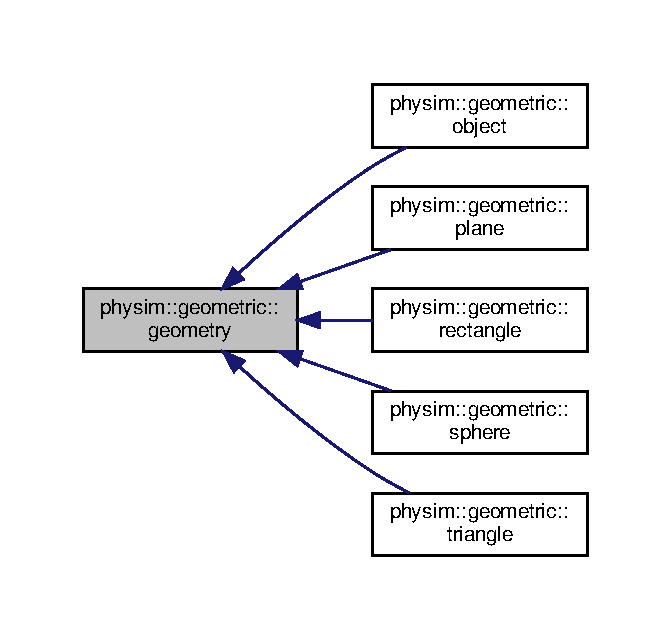
\includegraphics[width=322pt]{classphysim_1_1geometric_1_1geometry__inherit__graph}
\end{center}
\end{figure}


Collaboration diagram for physim\+:\+:geometric\+:\+:geometry\+:\nopagebreak
\begin{figure}[H]
\begin{center}
\leavevmode
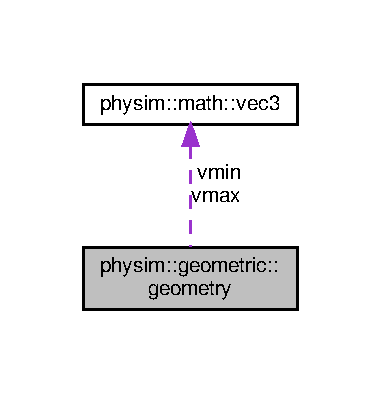
\includegraphics[width=183pt]{classphysim_1_1geometric_1_1geometry__coll__graph}
\end{center}
\end{figure}
\subsection*{Public Member Functions}
\begin{DoxyCompactItemize}
\item 
\mbox{\Hypertarget{classphysim_1_1geometric_1_1geometry_a79e4756803e45be5f1cfeb7d40668c7c}\label{classphysim_1_1geometric_1_1geometry_a79e4756803e45be5f1cfeb7d40668c7c}} 
\hyperlink{classphysim_1_1geometric_1_1geometry_a79e4756803e45be5f1cfeb7d40668c7c}{geometry} ()
\begin{DoxyCompactList}\small\item\em Default constructor. \end{DoxyCompactList}\item 
\mbox{\Hypertarget{classphysim_1_1geometric_1_1geometry_a9274693e558edca5464d1945eb26f327}\label{classphysim_1_1geometric_1_1geometry_a9274693e558edca5464d1945eb26f327}} 
\hyperlink{classphysim_1_1geometric_1_1geometry_a9274693e558edca5464d1945eb26f327}{geometry} (const \hyperlink{classphysim_1_1geometric_1_1geometry}{geometry} \&g)
\begin{DoxyCompactList}\small\item\em Copy constructor. \end{DoxyCompactList}\item 
\mbox{\Hypertarget{classphysim_1_1geometric_1_1geometry_a3ad710d087fd0edadb584ce22feb4d2b}\label{classphysim_1_1geometric_1_1geometry_a3ad710d087fd0edadb584ce22feb4d2b}} 
virtual \hyperlink{classphysim_1_1geometric_1_1geometry_a3ad710d087fd0edadb584ce22feb4d2b}{$\sim$geometry} ()
\begin{DoxyCompactList}\small\item\em Destructor. \end{DoxyCompactList}\item 
virtual void \hyperlink{classphysim_1_1geometric_1_1geometry_a5b029b5fa8e55847d5aa06b1d341c88c}{set\+\_\+position} (const \hyperlink{structphysim_1_1math_1_1vec3}{math\+::vec3} \&p)=0
\begin{DoxyCompactList}\small\item\em Sets the position of the geometry. \end{DoxyCompactList}\item 
\mbox{\Hypertarget{classphysim_1_1geometric_1_1geometry_afab4343665170b22328a3c46359de5d1}\label{classphysim_1_1geometric_1_1geometry_afab4343665170b22328a3c46359de5d1}} 
virtual \hyperlink{namespacephysim_1_1geometric_ac2794fff270c5b2ff4307f107a365fca}{geometry\+\_\+type} \hyperlink{classphysim_1_1geometric_1_1geometry_afab4343665170b22328a3c46359de5d1}{get\+\_\+geom\+\_\+type} () const
\begin{DoxyCompactList}\small\item\em Returns the type of geometry of this object. \end{DoxyCompactList}\item 
\mbox{\Hypertarget{classphysim_1_1geometric_1_1geometry_aa5ee497ba6c15da3be5087cab53f2754}\label{classphysim_1_1geometric_1_1geometry_aa5ee497ba6c15da3be5087cab53f2754}} 
const \hyperlink{structphysim_1_1math_1_1vec3}{math\+::vec3} \& \hyperlink{classphysim_1_1geometric_1_1geometry_aa5ee497ba6c15da3be5087cab53f2754}{get\+\_\+min} () const
\begin{DoxyCompactList}\small\item\em Returns point with mininum coordinate values. \end{DoxyCompactList}\item 
\mbox{\Hypertarget{classphysim_1_1geometric_1_1geometry_a6ab9de84b1241c1e82187efb0398ddb3}\label{classphysim_1_1geometric_1_1geometry_a6ab9de84b1241c1e82187efb0398ddb3}} 
const \hyperlink{structphysim_1_1math_1_1vec3}{math\+::vec3} \& \hyperlink{classphysim_1_1geometric_1_1geometry_a6ab9de84b1241c1e82187efb0398ddb3}{get\+\_\+max} () const
\begin{DoxyCompactList}\small\item\em Returns point with maxinum coordinate values. \end{DoxyCompactList}\item 
\mbox{\Hypertarget{classphysim_1_1geometric_1_1geometry_a5b82ef61d845a8dc4adf4ae97d39c312}\label{classphysim_1_1geometric_1_1geometry_a5b82ef61d845a8dc4adf4ae97d39c312}} 
\hyperlink{structphysim_1_1math_1_1vec3}{math\+::vec3} \hyperlink{classphysim_1_1geometric_1_1geometry_a5b82ef61d845a8dc4adf4ae97d39c312}{get\+\_\+box\+\_\+center} () const
\begin{DoxyCompactList}\small\item\em Returns the center of the bounding box. \end{DoxyCompactList}\item 
float \hyperlink{classphysim_1_1geometric_1_1geometry_a570de2d1faf50b787ec2f72703c41e19}{approx\+\_\+radius} () const
\begin{DoxyCompactList}\small\item\em Returns the radius of the bounding sphere. \end{DoxyCompactList}\item 
virtual bool \hyperlink{classphysim_1_1geometric_1_1geometry_a325d4049d4e14584b389a2f1202bdc08}{is\+\_\+inside} (const \hyperlink{structphysim_1_1math_1_1vec3}{math\+::vec3} \&p, float tol=1.e-\/6f) const =0
\begin{DoxyCompactList}\small\item\em Returns whether a point is inside the geometry. \end{DoxyCompactList}\item 
virtual bool \hyperlink{classphysim_1_1geometric_1_1geometry_a63d63c340937cede50a95903679c5ad3}{intersec\+\_\+segment} (const \hyperlink{structphysim_1_1math_1_1vec3}{math\+::vec3} \&p1, const \hyperlink{structphysim_1_1math_1_1vec3}{math\+::vec3} \&p2) const =0
\begin{DoxyCompactList}\small\item\em Returns if the segment defined by the points {\itshape p1} and {\itshape p2} intersects the geometry. \end{DoxyCompactList}\item 
virtual bool \hyperlink{classphysim_1_1geometric_1_1geometry_ae9fa877e89b7b2693a94d0772561ad9a}{intersec\+\_\+segment} (const \hyperlink{structphysim_1_1math_1_1vec3}{math\+::vec3} \&p1, const \hyperlink{structphysim_1_1math_1_1vec3}{math\+::vec3} \&p2, \hyperlink{structphysim_1_1math_1_1vec3}{math\+::vec3} \&p\+\_\+inter) const =0
\begin{DoxyCompactList}\small\item\em Returns true if the segment \mbox{[}{\itshape p1}, {\itshape p2} \mbox{]} intersects with the geometry. \end{DoxyCompactList}\item 
virtual bool \hyperlink{classphysim_1_1geometric_1_1geometry_aab49e452a72d1ecaf434be2b8de98169}{intersec\+\_\+sphere} (const \hyperlink{structphysim_1_1math_1_1vec3}{math\+::vec3} \&c, float R) const =0
\begin{DoxyCompactList}\small\item\em Returns if the sphere with center the point {\itshape c} and radius {\itshape R} intersects the geometry. \end{DoxyCompactList}\item 
virtual void \hyperlink{classphysim_1_1geometric_1_1geometry_ae5d606ba51451b964fcb2301d5622cab}{update\+\_\+particle} (const \hyperlink{structphysim_1_1math_1_1vec3}{math\+::vec3} \&pred\+\_\+pos, const \hyperlink{structphysim_1_1math_1_1vec3}{math\+::vec3} \&pred\+\_\+vel, \hyperlink{classphysim_1_1particles_1_1free__particle}{particles\+::free\+\_\+particle} \&pred) const =0
\begin{DoxyCompactList}\small\item\em Update a free particle in a collision with geometry. \end{DoxyCompactList}\item 
virtual void \hyperlink{classphysim_1_1geometric_1_1geometry_a11c26d2fea85bf7bc41ec94cefa9729e}{update\+\_\+particle} (const \hyperlink{structphysim_1_1math_1_1vec3}{math\+::vec3} \&pred\+\_\+pos, const \hyperlink{structphysim_1_1math_1_1vec3}{math\+::vec3} \&pred\+\_\+vel, \hyperlink{classphysim_1_1particles_1_1sized__particle}{particles\+::sized\+\_\+particle} \&pred) const =0
\begin{DoxyCompactList}\small\item\em Update a sized particle in a collision with geometry. \end{DoxyCompactList}\item 
\mbox{\Hypertarget{classphysim_1_1geometric_1_1geometry_a1fdaea58b350277f14ee51aedba3111e}\label{classphysim_1_1geometric_1_1geometry_a1fdaea58b350277f14ee51aedba3111e}} 
virtual void \hyperlink{classphysim_1_1geometric_1_1geometry_a1fdaea58b350277f14ee51aedba3111e}{display} () const =0
\begin{DoxyCompactList}\small\item\em Output on stream {\itshape cout} information about this geometry. \end{DoxyCompactList}\end{DoxyCompactItemize}
\subsection*{Protected Attributes}
\begin{DoxyCompactItemize}
\item 
\mbox{\Hypertarget{classphysim_1_1geometric_1_1geometry_a5a573b2ff467d2fe492db9240eeff49a}\label{classphysim_1_1geometric_1_1geometry_a5a573b2ff467d2fe492db9240eeff49a}} 
\hyperlink{structphysim_1_1math_1_1vec3}{math\+::vec3} \hyperlink{classphysim_1_1geometric_1_1geometry_a5a573b2ff467d2fe492db9240eeff49a}{vmin}
\begin{DoxyCompactList}\small\item\em Minimum coordinates of the geometry. \end{DoxyCompactList}\item 
\mbox{\Hypertarget{classphysim_1_1geometric_1_1geometry_a75eeb09e8584ff0d2109396baf0380d4}\label{classphysim_1_1geometric_1_1geometry_a75eeb09e8584ff0d2109396baf0380d4}} 
\hyperlink{structphysim_1_1math_1_1vec3}{math\+::vec3} \hyperlink{classphysim_1_1geometric_1_1geometry_a75eeb09e8584ff0d2109396baf0380d4}{vmax}
\begin{DoxyCompactList}\small\item\em Maximum coordinates of the geometry. \end{DoxyCompactList}\end{DoxyCompactItemize}


\subsection{Detailed Description}
All geometrical on the scene. 

This class is used to group all geometrical objects on the simulated scene.

These objects are typically spheres, planes, triangles that are fixed at a certain position.

Maybe they could also move, but not as a result of any collision between this object and another one. 

\subsection{Member Function Documentation}
\mbox{\Hypertarget{classphysim_1_1geometric_1_1geometry_a570de2d1faf50b787ec2f72703c41e19}\label{classphysim_1_1geometric_1_1geometry_a570de2d1faf50b787ec2f72703c41e19}} 
\index{physim\+::geometric\+::geometry@{physim\+::geometric\+::geometry}!approx\+\_\+radius@{approx\+\_\+radius}}
\index{approx\+\_\+radius@{approx\+\_\+radius}!physim\+::geometric\+::geometry@{physim\+::geometric\+::geometry}}
\subsubsection{\texorpdfstring{approx\+\_\+radius()}{approx\_radius()}}
{\footnotesize\ttfamily float physim\+::geometric\+::geometry\+::approx\+\_\+radius (\begin{DoxyParamCaption}{ }\end{DoxyParamCaption}) const}



Returns the radius of the bounding sphere. 

\begin{DoxyReturn}{Returns}
Returns the length between the center of the box and one of its vertices. 
\end{DoxyReturn}
\mbox{\Hypertarget{classphysim_1_1geometric_1_1geometry_a63d63c340937cede50a95903679c5ad3}\label{classphysim_1_1geometric_1_1geometry_a63d63c340937cede50a95903679c5ad3}} 
\index{physim\+::geometric\+::geometry@{physim\+::geometric\+::geometry}!intersec\+\_\+segment@{intersec\+\_\+segment}}
\index{intersec\+\_\+segment@{intersec\+\_\+segment}!physim\+::geometric\+::geometry@{physim\+::geometric\+::geometry}}
\subsubsection{\texorpdfstring{intersec\+\_\+segment()}{intersec\_segment()}\hspace{0.1cm}{\footnotesize\ttfamily [1/2]}}
{\footnotesize\ttfamily virtual bool physim\+::geometric\+::geometry\+::intersec\+\_\+segment (\begin{DoxyParamCaption}\item[{const \hyperlink{structphysim_1_1math_1_1vec3}{math\+::vec3} \&}]{p1,  }\item[{const \hyperlink{structphysim_1_1math_1_1vec3}{math\+::vec3} \&}]{p2 }\end{DoxyParamCaption}) const\hspace{0.3cm}{\ttfamily [pure virtual]}}



Returns if the segment defined by the points {\itshape p1} and {\itshape p2} intersects the geometry. 


\begin{DoxyParams}[1]{Parameters}
\mbox{\tt in}  & {\em p1} & First endpoint of the segment. \\
\hline
\mbox{\tt in}  & {\em p2} & Second endpoint of the segment. \\
\hline
\end{DoxyParams}
\begin{DoxyReturn}{Returns}
Returns true if there is intersection. 
\end{DoxyReturn}


Implemented in \hyperlink{classphysim_1_1geometric_1_1rectangle_aed45b841c7d1e615565e36720386f7a4}{physim\+::geometric\+::rectangle}, \hyperlink{classphysim_1_1geometric_1_1triangle_ab5ca57fd95a11b4fd1754d6d35799f23}{physim\+::geometric\+::triangle}, \hyperlink{classphysim_1_1geometric_1_1plane_a8a3b99b36271702bbececed5fce16391}{physim\+::geometric\+::plane}, \hyperlink{classphysim_1_1geometric_1_1object_a1bb905634af6176cc88680ce6f9fb080}{physim\+::geometric\+::object}, and \hyperlink{classphysim_1_1geometric_1_1sphere_ae9e58ed95da106650ca29f210d75223b}{physim\+::geometric\+::sphere}.

\mbox{\Hypertarget{classphysim_1_1geometric_1_1geometry_ae9fa877e89b7b2693a94d0772561ad9a}\label{classphysim_1_1geometric_1_1geometry_ae9fa877e89b7b2693a94d0772561ad9a}} 
\index{physim\+::geometric\+::geometry@{physim\+::geometric\+::geometry}!intersec\+\_\+segment@{intersec\+\_\+segment}}
\index{intersec\+\_\+segment@{intersec\+\_\+segment}!physim\+::geometric\+::geometry@{physim\+::geometric\+::geometry}}
\subsubsection{\texorpdfstring{intersec\+\_\+segment()}{intersec\_segment()}\hspace{0.1cm}{\footnotesize\ttfamily [2/2]}}
{\footnotesize\ttfamily virtual bool physim\+::geometric\+::geometry\+::intersec\+\_\+segment (\begin{DoxyParamCaption}\item[{const \hyperlink{structphysim_1_1math_1_1vec3}{math\+::vec3} \&}]{p1,  }\item[{const \hyperlink{structphysim_1_1math_1_1vec3}{math\+::vec3} \&}]{p2,  }\item[{\hyperlink{structphysim_1_1math_1_1vec3}{math\+::vec3} \&}]{p\+\_\+inter }\end{DoxyParamCaption}) const\hspace{0.3cm}{\ttfamily [pure virtual]}}



Returns true if the segment \mbox{[}{\itshape p1}, {\itshape p2} \mbox{]} intersects with the geometry. 


\begin{DoxyParams}[1]{Parameters}
\mbox{\tt in}  & {\em p1} & The first endpoint of the segment. \\
\hline
\mbox{\tt in}  & {\em p2} & The second endpoint of the segment. \\
\hline
\mbox{\tt out}  & {\em p\+\_\+inter} & The intersection point between the segment and the geometry. \\
\hline
\end{DoxyParams}
\begin{DoxyReturn}{Returns}
Returns true if the segment and the geometry intersect. In this case, the value in {\itshape p\+\_\+inter} will be the intersection point. 
\end{DoxyReturn}


Implemented in \hyperlink{classphysim_1_1geometric_1_1rectangle_a093865345b5a82576351be159ae56ee1}{physim\+::geometric\+::rectangle}, \hyperlink{classphysim_1_1geometric_1_1triangle_a013d124b88d40ddd698ed27047896bd0}{physim\+::geometric\+::triangle}, \hyperlink{classphysim_1_1geometric_1_1plane_a4e42f4d03045655690ee0339a9f2b50d}{physim\+::geometric\+::plane}, \hyperlink{classphysim_1_1geometric_1_1object_a10ee0f5a42edf3c469a9354a11571aac}{physim\+::geometric\+::object}, and \hyperlink{classphysim_1_1geometric_1_1sphere_ac89b9985569693cb7f6ba6cb3d0fe9f8}{physim\+::geometric\+::sphere}.

\mbox{\Hypertarget{classphysim_1_1geometric_1_1geometry_aab49e452a72d1ecaf434be2b8de98169}\label{classphysim_1_1geometric_1_1geometry_aab49e452a72d1ecaf434be2b8de98169}} 
\index{physim\+::geometric\+::geometry@{physim\+::geometric\+::geometry}!intersec\+\_\+sphere@{intersec\+\_\+sphere}}
\index{intersec\+\_\+sphere@{intersec\+\_\+sphere}!physim\+::geometric\+::geometry@{physim\+::geometric\+::geometry}}
\subsubsection{\texorpdfstring{intersec\+\_\+sphere()}{intersec\_sphere()}}
{\footnotesize\ttfamily virtual bool physim\+::geometric\+::geometry\+::intersec\+\_\+sphere (\begin{DoxyParamCaption}\item[{const \hyperlink{structphysim_1_1math_1_1vec3}{math\+::vec3} \&}]{c,  }\item[{float}]{R }\end{DoxyParamCaption}) const\hspace{0.3cm}{\ttfamily [pure virtual]}}



Returns if the sphere with center the point {\itshape c} and radius {\itshape R} intersects the geometry. 


\begin{DoxyParams}[1]{Parameters}
\mbox{\tt in}  & {\em c} & Center of the sphere. \\
\hline
\mbox{\tt in}  & {\em R} & radius of the sphere. \\
\hline
\end{DoxyParams}
\begin{DoxyReturn}{Returns}
Returns true if there is intersection. 
\end{DoxyReturn}


Implemented in \hyperlink{classphysim_1_1geometric_1_1rectangle_a39a293ca40cfbde7a2ef8c1ab487833d}{physim\+::geometric\+::rectangle}, \hyperlink{classphysim_1_1geometric_1_1triangle_a0cb72d1f970ef06df43206eb4b9cf19a}{physim\+::geometric\+::triangle}, \hyperlink{classphysim_1_1geometric_1_1plane_a1f4ba9f73933f56201339789e37f7ff7}{physim\+::geometric\+::plane}, \hyperlink{classphysim_1_1geometric_1_1object_a2846f76ef5b800bc50b6fa7e0a478a80}{physim\+::geometric\+::object}, and \hyperlink{classphysim_1_1geometric_1_1sphere_ad0f0fb96457cef20bb6626cad129b90b}{physim\+::geometric\+::sphere}.

\mbox{\Hypertarget{classphysim_1_1geometric_1_1geometry_a325d4049d4e14584b389a2f1202bdc08}\label{classphysim_1_1geometric_1_1geometry_a325d4049d4e14584b389a2f1202bdc08}} 
\index{physim\+::geometric\+::geometry@{physim\+::geometric\+::geometry}!is\+\_\+inside@{is\+\_\+inside}}
\index{is\+\_\+inside@{is\+\_\+inside}!physim\+::geometric\+::geometry@{physim\+::geometric\+::geometry}}
\subsubsection{\texorpdfstring{is\+\_\+inside()}{is\_inside()}}
{\footnotesize\ttfamily virtual bool physim\+::geometric\+::geometry\+::is\+\_\+inside (\begin{DoxyParamCaption}\item[{const \hyperlink{structphysim_1_1math_1_1vec3}{math\+::vec3} \&}]{p,  }\item[{float}]{tol = {\ttfamily 1.e-\/6f} }\end{DoxyParamCaption}) const\hspace{0.3cm}{\ttfamily [pure virtual]}}



Returns whether a point is inside the geometry. 


\begin{DoxyParams}{Parameters}
{\em p} & The point to check whether it is inside the geometry. \\
\hline
{\em tol} & Optional tolerance to deal corerctly with equalities. \\
\hline
\end{DoxyParams}
\begin{DoxyReturn}{Returns}
Returns true if {\itshape p} is inside the geometry. Returns false if otherwise. Depending on the type of geometry this method has a different geometrical interpretation. 
\end{DoxyReturn}


Implemented in \hyperlink{classphysim_1_1geometric_1_1rectangle_ab36400ef3f750fb6482fda8e1044bfa5}{physim\+::geometric\+::rectangle}, \hyperlink{classphysim_1_1geometric_1_1triangle_a735cfae7db71f5d6105011c40595ca37}{physim\+::geometric\+::triangle}, \hyperlink{classphysim_1_1geometric_1_1plane_a873ac41caf2d1ed4b9f8e52502ecbd92}{physim\+::geometric\+::plane}, \hyperlink{classphysim_1_1geometric_1_1object_ade3bdbcb865c6b0910b8adfe2225be9b}{physim\+::geometric\+::object}, and \hyperlink{classphysim_1_1geometric_1_1sphere_a22ca74b7056f85165d80d9913b32bbfb}{physim\+::geometric\+::sphere}.

\mbox{\Hypertarget{classphysim_1_1geometric_1_1geometry_a5b029b5fa8e55847d5aa06b1d341c88c}\label{classphysim_1_1geometric_1_1geometry_a5b029b5fa8e55847d5aa06b1d341c88c}} 
\index{physim\+::geometric\+::geometry@{physim\+::geometric\+::geometry}!set\+\_\+position@{set\+\_\+position}}
\index{set\+\_\+position@{set\+\_\+position}!physim\+::geometric\+::geometry@{physim\+::geometric\+::geometry}}
\subsubsection{\texorpdfstring{set\+\_\+position()}{set\_position()}}
{\footnotesize\ttfamily virtual void physim\+::geometric\+::geometry\+::set\+\_\+position (\begin{DoxyParamCaption}\item[{const \hyperlink{structphysim_1_1math_1_1vec3}{math\+::vec3} \&}]{p }\end{DoxyParamCaption})\hspace{0.3cm}{\ttfamily [pure virtual]}}



Sets the position of the geometry. 

For each type of object that implements this class, setting the position has a different geometrical interpretation. 
\begin{DoxyParams}{Parameters}
{\em p} & The \char`\"{}new position\char`\"{} of the object. \\
\hline
\end{DoxyParams}


Implemented in \hyperlink{classphysim_1_1geometric_1_1rectangle_a7458e8b880ace6a3393a728edb6d66fa}{physim\+::geometric\+::rectangle}, \hyperlink{classphysim_1_1geometric_1_1triangle_a60c60f0260fff5402c546a01e7fb5d5f}{physim\+::geometric\+::triangle}, \hyperlink{classphysim_1_1geometric_1_1plane_a201455ce1b4493b02b2f0c14e7d57e71}{physim\+::geometric\+::plane}, \hyperlink{classphysim_1_1geometric_1_1sphere_ad31c556961c46dbbdf3ade9bd7035d58}{physim\+::geometric\+::sphere}, and \hyperlink{classphysim_1_1geometric_1_1object_ab1efcebf4013206cee817beeb0415cd6}{physim\+::geometric\+::object}.

\mbox{\Hypertarget{classphysim_1_1geometric_1_1geometry_ae5d606ba51451b964fcb2301d5622cab}\label{classphysim_1_1geometric_1_1geometry_ae5d606ba51451b964fcb2301d5622cab}} 
\index{physim\+::geometric\+::geometry@{physim\+::geometric\+::geometry}!update\+\_\+particle@{update\+\_\+particle}}
\index{update\+\_\+particle@{update\+\_\+particle}!physim\+::geometric\+::geometry@{physim\+::geometric\+::geometry}}
\subsubsection{\texorpdfstring{update\+\_\+particle()}{update\_particle()}\hspace{0.1cm}{\footnotesize\ttfamily [1/2]}}
{\footnotesize\ttfamily virtual void physim\+::geometric\+::geometry\+::update\+\_\+particle (\begin{DoxyParamCaption}\item[{const \hyperlink{structphysim_1_1math_1_1vec3}{math\+::vec3} \&}]{pred\+\_\+pos,  }\item[{const \hyperlink{structphysim_1_1math_1_1vec3}{math\+::vec3} \&}]{pred\+\_\+vel,  }\item[{\hyperlink{classphysim_1_1particles_1_1free__particle}{particles\+::free\+\_\+particle} \&}]{pred }\end{DoxyParamCaption}) const\hspace{0.3cm}{\ttfamily [pure virtual]}}



Update a free particle in a collision with geometry. 

Assumig that particle {\itshape pred} collided with this geometry, update its position, velocity, ... accordingly.

For example, some geometry may be \textquotesingle{}bouncy\textquotesingle{}, it may give the particle some extra speed. This needs to be updated in this method.

The particle {\itshape pred} is given in a state that is not modified by any solver. That is, the particle\textquotesingle{}s position, velocity, force, ... have the value at time step {\itshape T}. The predicted position and velocity are given in {\itshape pred\+\_\+pos} and {\itshape pred\+\_\+vel}. These are predictions of the position and velocity for time {\itshape T} + {\itshape dt} (where dt is some time step). The modified particle due to the collision must be stored in {\itshape pred}.

This method is called only when it is sure that there has been a collision\+: the segment joining the particle\textquotesingle{}s current position and the predicted position intersects the geometry.


\begin{DoxyParams}[1]{Parameters}
\mbox{\tt in}  & {\em pred\+\_\+pos} & The predicted position of the particle. \\
\hline
\mbox{\tt in}  & {\em pred\+\_\+vel} & The predicted velocity of the particle. \\
\hline
\mbox{\tt out}  & {\em pred} & The particle with the result of the collision. \\
\hline
\end{DoxyParams}


Implemented in \hyperlink{classphysim_1_1geometric_1_1rectangle_a38e4eaa8bff24511cd3a9d94cd04e3dd}{physim\+::geometric\+::rectangle}, \hyperlink{classphysim_1_1geometric_1_1triangle_a3285ad4d763703ed84a21b25420c84bc}{physim\+::geometric\+::triangle}, \hyperlink{classphysim_1_1geometric_1_1plane_a9dc212ff39713d1525550c0bf328fe3a}{physim\+::geometric\+::plane}, \hyperlink{classphysim_1_1geometric_1_1object_a9885341b8bad60413402d84249bea9a2}{physim\+::geometric\+::object}, and \hyperlink{classphysim_1_1geometric_1_1sphere_a22318ec85e433ed92a0a9f90aed97b79}{physim\+::geometric\+::sphere}.

\mbox{\Hypertarget{classphysim_1_1geometric_1_1geometry_a11c26d2fea85bf7bc41ec94cefa9729e}\label{classphysim_1_1geometric_1_1geometry_a11c26d2fea85bf7bc41ec94cefa9729e}} 
\index{physim\+::geometric\+::geometry@{physim\+::geometric\+::geometry}!update\+\_\+particle@{update\+\_\+particle}}
\index{update\+\_\+particle@{update\+\_\+particle}!physim\+::geometric\+::geometry@{physim\+::geometric\+::geometry}}
\subsubsection{\texorpdfstring{update\+\_\+particle()}{update\_particle()}\hspace{0.1cm}{\footnotesize\ttfamily [2/2]}}
{\footnotesize\ttfamily virtual void physim\+::geometric\+::geometry\+::update\+\_\+particle (\begin{DoxyParamCaption}\item[{const \hyperlink{structphysim_1_1math_1_1vec3}{math\+::vec3} \&}]{pred\+\_\+pos,  }\item[{const \hyperlink{structphysim_1_1math_1_1vec3}{math\+::vec3} \&}]{pred\+\_\+vel,  }\item[{\hyperlink{classphysim_1_1particles_1_1sized__particle}{particles\+::sized\+\_\+particle} \&}]{pred }\end{DoxyParamCaption}) const\hspace{0.3cm}{\ttfamily [pure virtual]}}



Update a sized particle in a collision with geometry. 

Assumig that particle {\itshape pred} collided with this geometry, update its position, velocity, ... accordingly.

For example, some geometry may be \textquotesingle{}bouncy\textquotesingle{}, it may give the particle some extra speed. This needs to be updated in this method.

The particle {\itshape pred} is given in a state that is not modified by any solver. That is, the particle\textquotesingle{}s position, velocity, force, ... have the value at time step {\itshape T}. The predicted position and velocity are given in {\itshape pred\+\_\+pos} and {\itshape pred\+\_\+vel}. These are predictions of the position and velocity for time {\itshape T} + {\itshape dt} (where dt is some time step). The modified particle due to the collision must be stored in {\itshape pred}.

This method is called only when it is sure that there has been a collision\+: the segment joining the particle\textquotesingle{}s current position and the predicted position intersects the geometry.


\begin{DoxyParams}[1]{Parameters}
\mbox{\tt in}  & {\em pred\+\_\+pos} & The predicted position of the particle. \\
\hline
\mbox{\tt in}  & {\em pred\+\_\+vel} & The predicted velocity of the particle. \\
\hline
\mbox{\tt out}  & {\em pred} & The particle with the result of the collision. \\
\hline
\end{DoxyParams}


Implemented in \hyperlink{classphysim_1_1geometric_1_1rectangle_a61fead9b22595c9d9be8dc3867e26717}{physim\+::geometric\+::rectangle}, \hyperlink{classphysim_1_1geometric_1_1triangle_ae2551793ce8a5de01504326309c1543b}{physim\+::geometric\+::triangle}, \hyperlink{classphysim_1_1geometric_1_1plane_aff9bd840500b32eeefb89ac0a7d9b95f}{physim\+::geometric\+::plane}, \hyperlink{classphysim_1_1geometric_1_1object_aa9f27d1cc4ee3a3b9883bd155435c2bc}{physim\+::geometric\+::object}, and \hyperlink{classphysim_1_1geometric_1_1sphere_a3c395dccc5e2c8995e28767419fe59d6}{physim\+::geometric\+::sphere}.



The documentation for this class was generated from the following files\+:\begin{DoxyCompactItemize}
\item 
physim/geometry/geometry.\+hpp\item 
physim/geometry/geometry.\+cpp\end{DoxyCompactItemize}

\hypertarget{classphysim_1_1fields_1_1gravitational}{}\section{physim\+:\+:fields\+:\+:gravitational Class Reference}
\label{classphysim_1_1fields_1_1gravitational}\index{physim\+::fields\+::gravitational@{physim\+::fields\+::gravitational}}


Gravitational field.  




{\ttfamily \#include $<$gravitational.\+hpp$>$}



Inheritance diagram for physim\+:\+:fields\+:\+:gravitational\+:\nopagebreak
\begin{figure}[H]
\begin{center}
\leavevmode
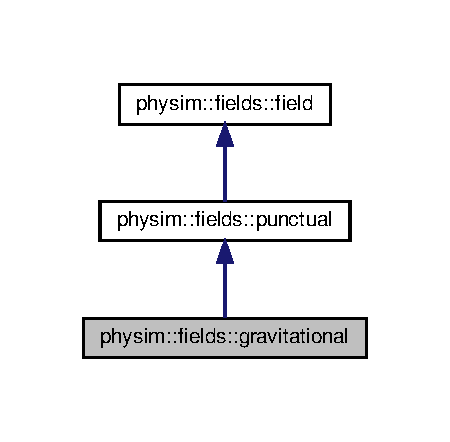
\includegraphics[width=216pt]{classphysim_1_1fields_1_1gravitational__inherit__graph}
\end{center}
\end{figure}


Collaboration diagram for physim\+:\+:fields\+:\+:gravitational\+:\nopagebreak
\begin{figure}[H]
\begin{center}
\leavevmode
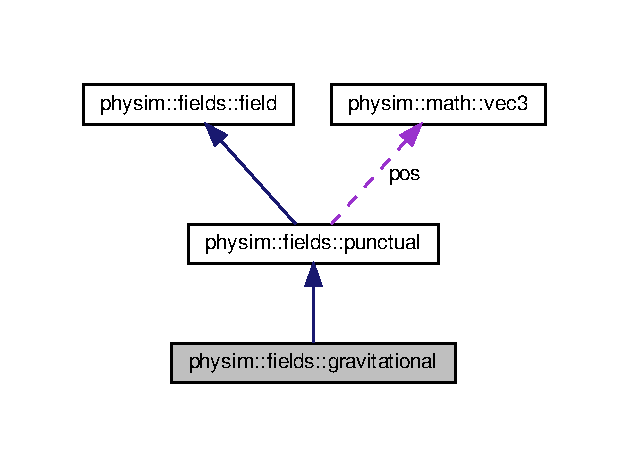
\includegraphics[width=302pt]{classphysim_1_1fields_1_1gravitational__coll__graph}
\end{center}
\end{figure}
\subsection*{Public Member Functions}
\begin{DoxyCompactItemize}
\item 
\mbox{\Hypertarget{classphysim_1_1fields_1_1gravitational_a55812f428aa2042618a8e4a0864725d3}\label{classphysim_1_1fields_1_1gravitational_a55812f428aa2042618a8e4a0864725d3}} 
\hyperlink{classphysim_1_1fields_1_1gravitational_a55812f428aa2042618a8e4a0864725d3}{gravitational} ()
\begin{DoxyCompactList}\small\item\em Default constructor. \end{DoxyCompactList}\item 
\mbox{\Hypertarget{classphysim_1_1fields_1_1gravitational_a679376bc3111cb91beea7b0ffd19fdab}\label{classphysim_1_1fields_1_1gravitational_a679376bc3111cb91beea7b0ffd19fdab}} 
\hyperlink{classphysim_1_1fields_1_1gravitational_a679376bc3111cb91beea7b0ffd19fdab}{gravitational} (const \hyperlink{structphysim_1_1math_1_1vec3}{math\+::vec3} \&\hyperlink{classphysim_1_1fields_1_1punctual_a00344d6f3e4f3f841e7d876918c66977}{pos}, float \hyperlink{classphysim_1_1fields_1_1gravitational_a0094aa217397b429bd807d6c630ec331}{M})
\begin{DoxyCompactList}\small\item\em Constructor with position and mass. \end{DoxyCompactList}\item 
\mbox{\Hypertarget{classphysim_1_1fields_1_1gravitational_a0e84ea687930b05ea072a77909053de5}\label{classphysim_1_1fields_1_1gravitational_a0e84ea687930b05ea072a77909053de5}} 
\hyperlink{classphysim_1_1fields_1_1gravitational_a0e84ea687930b05ea072a77909053de5}{gravitational} (const \hyperlink{classphysim_1_1fields_1_1gravitational}{gravitational} \&f)
\begin{DoxyCompactList}\small\item\em Copy constructor. \end{DoxyCompactList}\item 
\mbox{\Hypertarget{classphysim_1_1fields_1_1gravitational_a2b3c3ea8ae81a6dafac98b4f873065fe}\label{classphysim_1_1fields_1_1gravitational_a2b3c3ea8ae81a6dafac98b4f873065fe}} 
virtual \hyperlink{classphysim_1_1fields_1_1gravitational_a2b3c3ea8ae81a6dafac98b4f873065fe}{$\sim$gravitational} ()
\begin{DoxyCompactList}\small\item\em Destructor. \end{DoxyCompactList}\item 
\mbox{\Hypertarget{classphysim_1_1fields_1_1gravitational_a818cfac517c4d0469d9c0c9e54416685}\label{classphysim_1_1fields_1_1gravitational_a818cfac517c4d0469d9c0c9e54416685}} 
void \hyperlink{classphysim_1_1fields_1_1gravitational_a818cfac517c4d0469d9c0c9e54416685}{set\+\_\+mass} (float \hyperlink{classphysim_1_1fields_1_1gravitational_a0094aa217397b429bd807d6c630ec331}{M})
\begin{DoxyCompactList}\small\item\em Sets this gravitational field\textquotesingle{}s mass. See \hyperlink{classphysim_1_1fields_1_1gravitational_a0094aa217397b429bd807d6c630ec331}{M}. \end{DoxyCompactList}\item 
\mbox{\Hypertarget{classphysim_1_1fields_1_1gravitational_ae9b997278957311183a828800bdcbc6f}\label{classphysim_1_1fields_1_1gravitational_ae9b997278957311183a828800bdcbc6f}} 
float \hyperlink{classphysim_1_1fields_1_1gravitational_ae9b997278957311183a828800bdcbc6f}{get\+\_\+mass} () const
\begin{DoxyCompactList}\small\item\em Returns this field\textquotesingle{}s mass. See \hyperlink{classphysim_1_1fields_1_1gravitational_a0094aa217397b429bd807d6c630ec331}{M}. \end{DoxyCompactList}\item 
void \hyperlink{classphysim_1_1fields_1_1gravitational_af852abc69f07c67eb888fac9e7637693}{compute\+\_\+force} (const \hyperlink{classphysim_1_1particles_1_1free__particle}{particles\+::free\+\_\+particle} \&p, \hyperlink{structphysim_1_1math_1_1vec3}{math\+::vec3} \&F)
\begin{DoxyCompactList}\small\item\em Compute the force vector acting on a particle. \end{DoxyCompactList}\item 
void \hyperlink{classphysim_1_1fields_1_1gravitational_a2283f98ad0ce6732c81e744d3c2b898d}{compute\+\_\+force} (const \hyperlink{classphysim_1_1particles_1_1mesh__particle}{particles\+::mesh\+\_\+particle} \&p, \hyperlink{structphysim_1_1math_1_1vec3}{math\+::vec3} \&F)
\begin{DoxyCompactList}\small\item\em Compute the force vector acting on a particle. \end{DoxyCompactList}\item 
void \hyperlink{classphysim_1_1fields_1_1gravitational_a1b11432dfb9e1bc2720794304f224432}{compute\+\_\+force} (const \hyperlink{classphysim_1_1particles_1_1fluid__particle}{particles\+::fluid\+\_\+particle} \&p, \hyperlink{structphysim_1_1math_1_1vec3}{math\+::vec3} \&F)
\begin{DoxyCompactList}\small\item\em Compute the force vector acting on a particle. \end{DoxyCompactList}\end{DoxyCompactItemize}
\subsection*{Protected Attributes}
\begin{DoxyCompactItemize}
\item 
\mbox{\Hypertarget{classphysim_1_1fields_1_1gravitational_a0094aa217397b429bd807d6c630ec331}\label{classphysim_1_1fields_1_1gravitational_a0094aa217397b429bd807d6c630ec331}} 
float \hyperlink{classphysim_1_1fields_1_1gravitational_a0094aa217397b429bd807d6c630ec331}{M}
\begin{DoxyCompactList}\small\item\em Mass of object causing the gravitational field. \mbox{[}Kg\mbox{]}. \end{DoxyCompactList}\end{DoxyCompactItemize}
\subsection*{Private Member Functions}
\begin{DoxyCompactItemize}
\item 
{\footnotesize template$<$class P $>$ }\\void \hyperlink{classphysim_1_1fields_1_1gravitational_acb6baab17fcb3b3cbf61b6690bd935fd}{\+\_\+\+\_\+compute\+\_\+force} (const P \&p, \hyperlink{structphysim_1_1math_1_1vec3}{math\+::vec3} \&F)
\begin{DoxyCompactList}\small\item\em Function that actuall computes the force of this field. \end{DoxyCompactList}\end{DoxyCompactItemize}


\subsection{Detailed Description}
Gravitational field. 

This class implements the force that a gravitational field applies on a particle of mass m.

This gravitational field is caused by some body of mass \hyperlink{classphysim_1_1fields_1_1gravitational_a0094aa217397b429bd807d6c630ec331}{M}, at position \hyperlink{classphysim_1_1fields_1_1punctual_a00344d6f3e4f3f841e7d876918c66977}{punctual\+::pos}.

Therefore the force is computed using $-G \cdot M \cdot m \cdot \frac{p - O}{||p - O||}$ where
\begin{DoxyItemize}
\item $G$ is the gravitational constant.
\item $M$ is the mass of the particle causing the field.
\item $p$ is the particle\textquotesingle{}s position.
\item $O$ is the position of the particle causing the field. 
\end{DoxyItemize}

\subsection{Member Function Documentation}
\mbox{\Hypertarget{classphysim_1_1fields_1_1gravitational_acb6baab17fcb3b3cbf61b6690bd935fd}\label{classphysim_1_1fields_1_1gravitational_acb6baab17fcb3b3cbf61b6690bd935fd}} 
\index{physim\+::fields\+::gravitational@{physim\+::fields\+::gravitational}!\+\_\+\+\_\+compute\+\_\+force@{\+\_\+\+\_\+compute\+\_\+force}}
\index{\+\_\+\+\_\+compute\+\_\+force@{\+\_\+\+\_\+compute\+\_\+force}!physim\+::fields\+::gravitational@{physim\+::fields\+::gravitational}}
\subsubsection{\texorpdfstring{\+\_\+\+\_\+compute\+\_\+force()}{\_\_compute\_force()}}
{\footnotesize\ttfamily template$<$class P $>$ \\
void physim\+::fields\+::gravitational\+::\+\_\+\+\_\+compute\+\_\+force (\begin{DoxyParamCaption}\item[{const P \&}]{p,  }\item[{\hyperlink{structphysim_1_1math_1_1vec3}{math\+::vec3} \&}]{F }\end{DoxyParamCaption})\hspace{0.3cm}{\ttfamily [private]}}



Function that actuall computes the force of this field. 

Works for \hyperlink{classphysim_1_1particles_1_1free__particle}{particles\+::free\+\_\+particle} and \hyperlink{classphysim_1_1particles_1_1mesh__particle}{particles\+::mesh\+\_\+particle}. \mbox{\Hypertarget{classphysim_1_1fields_1_1gravitational_af852abc69f07c67eb888fac9e7637693}\label{classphysim_1_1fields_1_1gravitational_af852abc69f07c67eb888fac9e7637693}} 
\index{physim\+::fields\+::gravitational@{physim\+::fields\+::gravitational}!compute\+\_\+force@{compute\+\_\+force}}
\index{compute\+\_\+force@{compute\+\_\+force}!physim\+::fields\+::gravitational@{physim\+::fields\+::gravitational}}
\subsubsection{\texorpdfstring{compute\+\_\+force()}{compute\_force()}\hspace{0.1cm}{\footnotesize\ttfamily [1/3]}}
{\footnotesize\ttfamily void physim\+::fields\+::gravitational\+::compute\+\_\+force (\begin{DoxyParamCaption}\item[{const \hyperlink{classphysim_1_1particles_1_1free__particle}{particles\+::free\+\_\+particle} \&}]{p,  }\item[{\hyperlink{structphysim_1_1math_1_1vec3}{math\+::vec3} \&}]{F }\end{DoxyParamCaption})\hspace{0.3cm}{\ttfamily [virtual]}}



Compute the force vector acting on a particle. 

The contents of parameter {\itshape F} is undefined when calling this function, thus the contents should be overwritten. 
\begin{DoxyParams}[1]{Parameters}
\mbox{\tt in}  & {\em p} & Particle where the force is applied to. \\
\hline
\mbox{\tt out}  & {\em F} & The force from this field acting on the particle. \\
\hline
\end{DoxyParams}


Implements \hyperlink{classphysim_1_1fields_1_1field_a0d836756ac51a6a1e99d3c9a60310694}{physim\+::fields\+::field}.

\mbox{\Hypertarget{classphysim_1_1fields_1_1gravitational_a2283f98ad0ce6732c81e744d3c2b898d}\label{classphysim_1_1fields_1_1gravitational_a2283f98ad0ce6732c81e744d3c2b898d}} 
\index{physim\+::fields\+::gravitational@{physim\+::fields\+::gravitational}!compute\+\_\+force@{compute\+\_\+force}}
\index{compute\+\_\+force@{compute\+\_\+force}!physim\+::fields\+::gravitational@{physim\+::fields\+::gravitational}}
\subsubsection{\texorpdfstring{compute\+\_\+force()}{compute\_force()}\hspace{0.1cm}{\footnotesize\ttfamily [2/3]}}
{\footnotesize\ttfamily void physim\+::fields\+::gravitational\+::compute\+\_\+force (\begin{DoxyParamCaption}\item[{const \hyperlink{classphysim_1_1particles_1_1mesh__particle}{particles\+::mesh\+\_\+particle} \&}]{p,  }\item[{\hyperlink{structphysim_1_1math_1_1vec3}{math\+::vec3} \&}]{F }\end{DoxyParamCaption})\hspace{0.3cm}{\ttfamily [virtual]}}



Compute the force vector acting on a particle. 

The contents of parameter {\itshape F} is undefined when calling this function, thus the contents should be overwritten. 
\begin{DoxyParams}[1]{Parameters}
\mbox{\tt in}  & {\em p} & Particle where the force is applied to. \\
\hline
\mbox{\tt out}  & {\em F} & The force from this field acting on the particle. \\
\hline
\end{DoxyParams}


Implements \hyperlink{classphysim_1_1fields_1_1field_aa167d81f223daab47989168c9d3b8cb4}{physim\+::fields\+::field}.

\mbox{\Hypertarget{classphysim_1_1fields_1_1gravitational_a1b11432dfb9e1bc2720794304f224432}\label{classphysim_1_1fields_1_1gravitational_a1b11432dfb9e1bc2720794304f224432}} 
\index{physim\+::fields\+::gravitational@{physim\+::fields\+::gravitational}!compute\+\_\+force@{compute\+\_\+force}}
\index{compute\+\_\+force@{compute\+\_\+force}!physim\+::fields\+::gravitational@{physim\+::fields\+::gravitational}}
\subsubsection{\texorpdfstring{compute\+\_\+force()}{compute\_force()}\hspace{0.1cm}{\footnotesize\ttfamily [3/3]}}
{\footnotesize\ttfamily void physim\+::fields\+::gravitational\+::compute\+\_\+force (\begin{DoxyParamCaption}\item[{const \hyperlink{classphysim_1_1particles_1_1fluid__particle}{particles\+::fluid\+\_\+particle} \&}]{p,  }\item[{\hyperlink{structphysim_1_1math_1_1vec3}{math\+::vec3} \&}]{F }\end{DoxyParamCaption})\hspace{0.3cm}{\ttfamily [virtual]}}



Compute the force vector acting on a particle. 

The contents of parameter {\itshape F} is undefined when calling this function, thus the contents should be overwritten. 
\begin{DoxyParams}[1]{Parameters}
\mbox{\tt in}  & {\em p} & Particle where the force is applied to. \\
\hline
\mbox{\tt out}  & {\em F} & The force from this field acting on the particle. \\
\hline
\end{DoxyParams}


Implements \hyperlink{classphysim_1_1fields_1_1field_a099fb8b1dee7afae4610c6275432bc81}{physim\+::fields\+::field}.



The documentation for this class was generated from the following files\+:\begin{DoxyCompactItemize}
\item 
physim/fields/gravitational.\+hpp\item 
physim/fields/gravitational.\+cpp\end{DoxyCompactItemize}

\hypertarget{classphysim_1_1fields_1_1gravitational__planet}{}\section{physim\+:\+:fields\+:\+:gravitational\+\_\+planet Class Reference}
\label{classphysim_1_1fields_1_1gravitational__planet}\index{physim\+::fields\+::gravitational\+\_\+planet@{physim\+::fields\+::gravitational\+\_\+planet}}


A planet\textquotesingle{}s gravitational field.  




{\ttfamily \#include $<$gravitational\+\_\+planet.\+hpp$>$}



Inheritance diagram for physim\+:\+:fields\+:\+:gravitational\+\_\+planet\+:\nopagebreak
\begin{figure}[H]
\begin{center}
\leavevmode
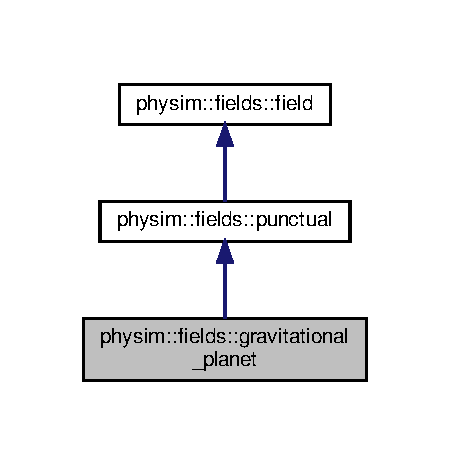
\includegraphics[width=216pt]{classphysim_1_1fields_1_1gravitational__planet__inherit__graph}
\end{center}
\end{figure}


Collaboration diagram for physim\+:\+:fields\+:\+:gravitational\+\_\+planet\+:\nopagebreak
\begin{figure}[H]
\begin{center}
\leavevmode
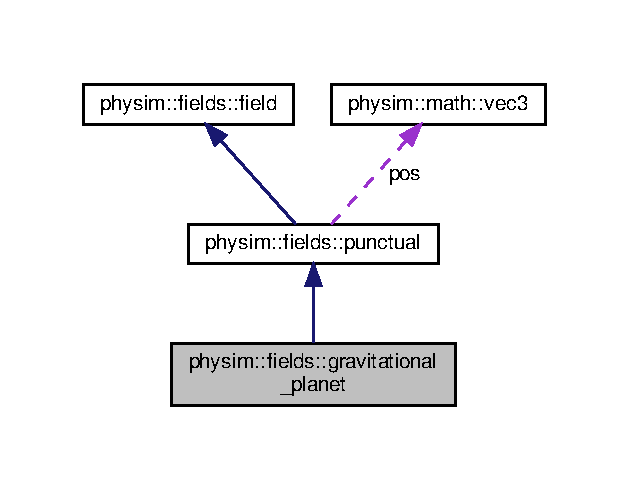
\includegraphics[width=302pt]{classphysim_1_1fields_1_1gravitational__planet__coll__graph}
\end{center}
\end{figure}
\subsection*{Public Member Functions}
\begin{DoxyCompactItemize}
\item 
\mbox{\Hypertarget{classphysim_1_1fields_1_1gravitational__planet_a9c225658e7538b0b62cb3e5647dfc172}\label{classphysim_1_1fields_1_1gravitational__planet_a9c225658e7538b0b62cb3e5647dfc172}} 
\hyperlink{classphysim_1_1fields_1_1gravitational__planet_a9c225658e7538b0b62cb3e5647dfc172}{gravitational\+\_\+planet} ()
\begin{DoxyCompactList}\small\item\em Default constructor. \end{DoxyCompactList}\item 
\mbox{\Hypertarget{classphysim_1_1fields_1_1gravitational__planet_adf2de01f520960fe939e0943cfa3871e}\label{classphysim_1_1fields_1_1gravitational__planet_adf2de01f520960fe939e0943cfa3871e}} 
\hyperlink{classphysim_1_1fields_1_1gravitational__planet_adf2de01f520960fe939e0943cfa3871e}{gravitational\+\_\+planet} (const \hyperlink{structphysim_1_1math_1_1vec3}{math\+::vec3} \&\hyperlink{classphysim_1_1fields_1_1punctual_a00344d6f3e4f3f841e7d876918c66977}{pos})
\begin{DoxyCompactList}\small\item\em Constructor with position and mass. \end{DoxyCompactList}\item 
\mbox{\Hypertarget{classphysim_1_1fields_1_1gravitational__planet_a7e1ac5ee386422f3b02129cac5c17b4d}\label{classphysim_1_1fields_1_1gravitational__planet_a7e1ac5ee386422f3b02129cac5c17b4d}} 
\hyperlink{classphysim_1_1fields_1_1gravitational__planet_a7e1ac5ee386422f3b02129cac5c17b4d}{gravitational\+\_\+planet} (const \hyperlink{classphysim_1_1fields_1_1gravitational__planet}{gravitational\+\_\+planet} \&f)
\begin{DoxyCompactList}\small\item\em Copy constructor. \end{DoxyCompactList}\item 
\mbox{\Hypertarget{classphysim_1_1fields_1_1gravitational__planet_a9384cf122e83c63992c000b221b9fb96}\label{classphysim_1_1fields_1_1gravitational__planet_a9384cf122e83c63992c000b221b9fb96}} 
virtual \hyperlink{classphysim_1_1fields_1_1gravitational__planet_a9384cf122e83c63992c000b221b9fb96}{$\sim$gravitational\+\_\+planet} ()
\begin{DoxyCompactList}\small\item\em Destructor. \end{DoxyCompactList}\item 
void \hyperlink{classphysim_1_1fields_1_1gravitational__planet_ab272f7db84ad53d320d467b75d3f9ed2}{compute\+\_\+force} (const \hyperlink{classphysim_1_1particles_1_1free__particle}{particles\+::free\+\_\+particle} \&p, \hyperlink{structphysim_1_1math_1_1vec3}{math\+::vec3} \&F)
\begin{DoxyCompactList}\small\item\em Compute the force vector acting on a particle. \end{DoxyCompactList}\item 
void \hyperlink{classphysim_1_1fields_1_1gravitational__planet_aece6e4cc8679b3be5075c1e5fd1b3162}{compute\+\_\+force} (const \hyperlink{classphysim_1_1particles_1_1mesh__particle}{particles\+::mesh\+\_\+particle} \&p, \hyperlink{structphysim_1_1math_1_1vec3}{math\+::vec3} \&F)
\begin{DoxyCompactList}\small\item\em Compute the force vector acting on a particle. \end{DoxyCompactList}\item 
void \hyperlink{classphysim_1_1fields_1_1gravitational__planet_a3b79869e1411c333b21ba4a240574641}{compute\+\_\+force} (const \hyperlink{classphysim_1_1particles_1_1fluid__particle}{particles\+::fluid\+\_\+particle} \&p, \hyperlink{structphysim_1_1math_1_1vec3}{math\+::vec3} \&F)
\begin{DoxyCompactList}\small\item\em Compute the force vector acting on a particle. \end{DoxyCompactList}\end{DoxyCompactItemize}
\subsection*{Private Member Functions}
\begin{DoxyCompactItemize}
\item 
{\footnotesize template$<$class P $>$ }\\void \hyperlink{classphysim_1_1fields_1_1gravitational__planet_a5bb7992e6b6b03144262e0dfb3639f17}{\+\_\+\+\_\+compute\+\_\+force} (const P \&p, \hyperlink{structphysim_1_1math_1_1vec3}{math\+::vec3} \&F)
\begin{DoxyCompactList}\small\item\em Function that actuall computes the force of this field. \end{DoxyCompactList}\end{DoxyCompactItemize}
\subsection*{Additional Inherited Members}


\subsection{Detailed Description}
A planet\textquotesingle{}s gravitational field. 

This class implements the gravitational force field typical of a planet.

This field is assumed to have some huge mass, placed at some point near infinity in a certain direction. This vector is stored at the position to which this field is set to, and interpreted as the acceleration of the gravity it yields. Thus, the force it applies on a particle of mass $m$ is\+:

$\vec{F} = m\cdot \vec{g}$

Here $g$ is the vector set in \hyperlink{classphysim_1_1fields_1_1punctual_a00344d6f3e4f3f841e7d876918c66977}{punctual\+::pos}. 

\subsection{Member Function Documentation}
\mbox{\Hypertarget{classphysim_1_1fields_1_1gravitational__planet_a5bb7992e6b6b03144262e0dfb3639f17}\label{classphysim_1_1fields_1_1gravitational__planet_a5bb7992e6b6b03144262e0dfb3639f17}} 
\index{physim\+::fields\+::gravitational\+\_\+planet@{physim\+::fields\+::gravitational\+\_\+planet}!\+\_\+\+\_\+compute\+\_\+force@{\+\_\+\+\_\+compute\+\_\+force}}
\index{\+\_\+\+\_\+compute\+\_\+force@{\+\_\+\+\_\+compute\+\_\+force}!physim\+::fields\+::gravitational\+\_\+planet@{physim\+::fields\+::gravitational\+\_\+planet}}
\subsubsection{\texorpdfstring{\+\_\+\+\_\+compute\+\_\+force()}{\_\_compute\_force()}}
{\footnotesize\ttfamily template$<$class P $>$ \\
void physim\+::fields\+::gravitational\+\_\+planet\+::\+\_\+\+\_\+compute\+\_\+force (\begin{DoxyParamCaption}\item[{const P \&}]{p,  }\item[{\hyperlink{structphysim_1_1math_1_1vec3}{math\+::vec3} \&}]{F }\end{DoxyParamCaption})\hspace{0.3cm}{\ttfamily [private]}}



Function that actuall computes the force of this field. 

Works for \hyperlink{classphysim_1_1particles_1_1free__particle}{particles\+::free\+\_\+particle} and \hyperlink{classphysim_1_1particles_1_1mesh__particle}{particles\+::mesh\+\_\+particle}. \mbox{\Hypertarget{classphysim_1_1fields_1_1gravitational__planet_ab272f7db84ad53d320d467b75d3f9ed2}\label{classphysim_1_1fields_1_1gravitational__planet_ab272f7db84ad53d320d467b75d3f9ed2}} 
\index{physim\+::fields\+::gravitational\+\_\+planet@{physim\+::fields\+::gravitational\+\_\+planet}!compute\+\_\+force@{compute\+\_\+force}}
\index{compute\+\_\+force@{compute\+\_\+force}!physim\+::fields\+::gravitational\+\_\+planet@{physim\+::fields\+::gravitational\+\_\+planet}}
\subsubsection{\texorpdfstring{compute\+\_\+force()}{compute\_force()}\hspace{0.1cm}{\footnotesize\ttfamily [1/3]}}
{\footnotesize\ttfamily void physim\+::fields\+::gravitational\+\_\+planet\+::compute\+\_\+force (\begin{DoxyParamCaption}\item[{const \hyperlink{classphysim_1_1particles_1_1free__particle}{particles\+::free\+\_\+particle} \&}]{p,  }\item[{\hyperlink{structphysim_1_1math_1_1vec3}{math\+::vec3} \&}]{F }\end{DoxyParamCaption})\hspace{0.3cm}{\ttfamily [virtual]}}



Compute the force vector acting on a particle. 

The contents of parameter {\itshape F} is undefined when calling this function, thus the contents should be overwritten. 
\begin{DoxyParams}[1]{Parameters}
\mbox{\tt in}  & {\em p} & Particle where the force is applied to. \\
\hline
\mbox{\tt out}  & {\em F} & The force from this field acting on the particle. \\
\hline
\end{DoxyParams}


Implements \hyperlink{classphysim_1_1fields_1_1field_a0d836756ac51a6a1e99d3c9a60310694}{physim\+::fields\+::field}.

\mbox{\Hypertarget{classphysim_1_1fields_1_1gravitational__planet_aece6e4cc8679b3be5075c1e5fd1b3162}\label{classphysim_1_1fields_1_1gravitational__planet_aece6e4cc8679b3be5075c1e5fd1b3162}} 
\index{physim\+::fields\+::gravitational\+\_\+planet@{physim\+::fields\+::gravitational\+\_\+planet}!compute\+\_\+force@{compute\+\_\+force}}
\index{compute\+\_\+force@{compute\+\_\+force}!physim\+::fields\+::gravitational\+\_\+planet@{physim\+::fields\+::gravitational\+\_\+planet}}
\subsubsection{\texorpdfstring{compute\+\_\+force()}{compute\_force()}\hspace{0.1cm}{\footnotesize\ttfamily [2/3]}}
{\footnotesize\ttfamily void physim\+::fields\+::gravitational\+\_\+planet\+::compute\+\_\+force (\begin{DoxyParamCaption}\item[{const \hyperlink{classphysim_1_1particles_1_1mesh__particle}{particles\+::mesh\+\_\+particle} \&}]{p,  }\item[{\hyperlink{structphysim_1_1math_1_1vec3}{math\+::vec3} \&}]{F }\end{DoxyParamCaption})\hspace{0.3cm}{\ttfamily [virtual]}}



Compute the force vector acting on a particle. 

The contents of parameter {\itshape F} is undefined when calling this function, thus the contents should be overwritten. 
\begin{DoxyParams}[1]{Parameters}
\mbox{\tt in}  & {\em p} & Particle where the force is applied to. \\
\hline
\mbox{\tt out}  & {\em F} & The force from this field acting on the particle. \\
\hline
\end{DoxyParams}


Implements \hyperlink{classphysim_1_1fields_1_1field_aa167d81f223daab47989168c9d3b8cb4}{physim\+::fields\+::field}.

\mbox{\Hypertarget{classphysim_1_1fields_1_1gravitational__planet_a3b79869e1411c333b21ba4a240574641}\label{classphysim_1_1fields_1_1gravitational__planet_a3b79869e1411c333b21ba4a240574641}} 
\index{physim\+::fields\+::gravitational\+\_\+planet@{physim\+::fields\+::gravitational\+\_\+planet}!compute\+\_\+force@{compute\+\_\+force}}
\index{compute\+\_\+force@{compute\+\_\+force}!physim\+::fields\+::gravitational\+\_\+planet@{physim\+::fields\+::gravitational\+\_\+planet}}
\subsubsection{\texorpdfstring{compute\+\_\+force()}{compute\_force()}\hspace{0.1cm}{\footnotesize\ttfamily [3/3]}}
{\footnotesize\ttfamily void physim\+::fields\+::gravitational\+\_\+planet\+::compute\+\_\+force (\begin{DoxyParamCaption}\item[{const \hyperlink{classphysim_1_1particles_1_1fluid__particle}{particles\+::fluid\+\_\+particle} \&}]{p,  }\item[{\hyperlink{structphysim_1_1math_1_1vec3}{math\+::vec3} \&}]{F }\end{DoxyParamCaption})\hspace{0.3cm}{\ttfamily [virtual]}}



Compute the force vector acting on a particle. 

The contents of parameter {\itshape F} is undefined when calling this function, thus the contents should be overwritten. 
\begin{DoxyParams}[1]{Parameters}
\mbox{\tt in}  & {\em p} & Particle where the force is applied to. \\
\hline
\mbox{\tt out}  & {\em F} & The force from this field acting on the particle. \\
\hline
\end{DoxyParams}


Implements \hyperlink{classphysim_1_1fields_1_1field_a099fb8b1dee7afae4610c6275432bc81}{physim\+::fields\+::field}.



The documentation for this class was generated from the following files\+:\begin{DoxyCompactItemize}
\item 
physim/fields/gravitational\+\_\+planet.\+hpp\item 
physim/fields/gravitational\+\_\+planet.\+cpp\end{DoxyCompactItemize}

\hypertarget{classphysim_1_1emitters_1_1free__emitters_1_1hose}{}\section{physim\+:\+:emitters\+:\+:free\+\_\+emitters\+:\+:hose Class Reference}
\label{classphysim_1_1emitters_1_1free__emitters_1_1hose}\index{physim\+::emitters\+::free\+\_\+emitters\+::hose@{physim\+::emitters\+::free\+\_\+emitters\+::hose}}


A hose emitter.  




{\ttfamily \#include $<$hose.\+hpp$>$}



Inheritance diagram for physim\+:\+:emitters\+:\+:free\+\_\+emitters\+:\+:hose\+:\nopagebreak
\begin{figure}[H]
\begin{center}
\leavevmode
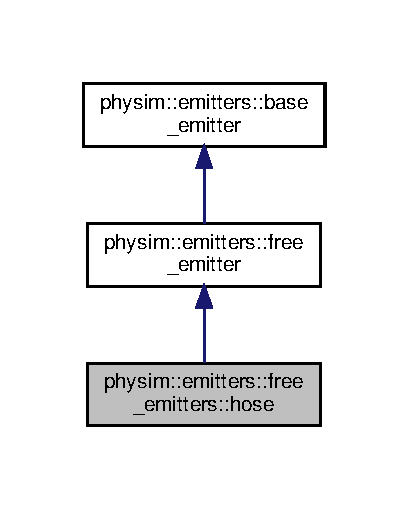
\includegraphics[width=196pt]{classphysim_1_1emitters_1_1free__emitters_1_1hose__inherit__graph}
\end{center}
\end{figure}


Collaboration diagram for physim\+:\+:emitters\+:\+:free\+\_\+emitters\+:\+:hose\+:\nopagebreak
\begin{figure}[H]
\begin{center}
\leavevmode
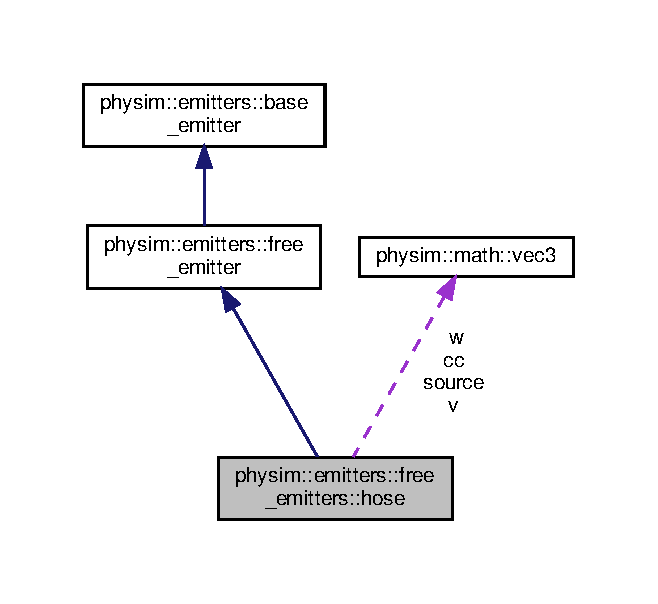
\includegraphics[width=316pt]{classphysim_1_1emitters_1_1free__emitters_1_1hose__coll__graph}
\end{center}
\end{figure}
\subsection*{Public Member Functions}
\begin{DoxyCompactItemize}
\item 
\mbox{\Hypertarget{classphysim_1_1emitters_1_1free__emitters_1_1hose_ae69ff0689f1e36850e034a508e84326f}\label{classphysim_1_1emitters_1_1free__emitters_1_1hose_ae69ff0689f1e36850e034a508e84326f}} 
\hyperlink{classphysim_1_1emitters_1_1free__emitters_1_1hose_ae69ff0689f1e36850e034a508e84326f}{hose} ()
\begin{DoxyCompactList}\small\item\em Default constructor. \end{DoxyCompactList}\item 
\hyperlink{classphysim_1_1emitters_1_1free__emitters_1_1hose_ad20ae14c9c19227c1555fa9ce7f58891}{hose} (const \hyperlink{classphysim_1_1emitters_1_1free__emitters_1_1hose}{hose} \&\hyperlink{classphysim_1_1emitters_1_1free__emitters_1_1hose_ac1398640d981dd745b8d26e72bc7fe40}{h})
\begin{DoxyCompactList}\small\item\em Copy constructor. \end{DoxyCompactList}\item 
\mbox{\Hypertarget{classphysim_1_1emitters_1_1free__emitters_1_1hose_a7063d70c22e19a7191067089f654d64d}\label{classphysim_1_1emitters_1_1free__emitters_1_1hose_a7063d70c22e19a7191067089f654d64d}} 
virtual \hyperlink{classphysim_1_1emitters_1_1free__emitters_1_1hose_a7063d70c22e19a7191067089f654d64d}{$\sim$hose} ()
\begin{DoxyCompactList}\small\item\em Destructor. \end{DoxyCompactList}\item 
void \hyperlink{classphysim_1_1emitters_1_1free__emitters_1_1hose_aeffa7bc72509d3ae1262244815f97737}{set\+\_\+hose\+\_\+source} (const \hyperlink{structphysim_1_1math_1_1vec3}{math\+::vec3} \&S, const \hyperlink{structphysim_1_1math_1_1vec3}{math\+::vec3} \&u, float \+\_\+r, float \+\_\+h)
\begin{DoxyCompactList}\small\item\em Sets the source of the hose. \end{DoxyCompactList}\item 
\mbox{\Hypertarget{classphysim_1_1emitters_1_1free__emitters_1_1hose_a31a261d8cb387f018faaf070eb5aef1a}\label{classphysim_1_1emitters_1_1free__emitters_1_1hose_a31a261d8cb387f018faaf070eb5aef1a}} 
\hyperlink{classphysim_1_1emitters_1_1free__emitter}{free\+\_\+emitter} $\ast$ \hyperlink{classphysim_1_1emitters_1_1free__emitters_1_1hose_a31a261d8cb387f018faaf070eb5aef1a}{clone} () const
\begin{DoxyCompactList}\small\item\em Returns a reference to a copy of this emitter. \end{DoxyCompactList}\end{DoxyCompactItemize}
\subsection*{Protected Member Functions}
\begin{DoxyCompactItemize}
\item 
virtual void \hyperlink{classphysim_1_1emitters_1_1free__emitters_1_1hose_a6c78d604106eb5b8d20021f56f9512ba}{make\+\_\+pos\+\_\+init} ()
\begin{DoxyCompactList}\small\item\em Sets the position initialser. \end{DoxyCompactList}\item 
virtual void \hyperlink{classphysim_1_1emitters_1_1free__emitters_1_1hose_a7976365f9101e4095d00dc8eafc82ebb}{make\+\_\+vel\+\_\+init} ()
\begin{DoxyCompactList}\small\item\em Sets the velocity initialser. \end{DoxyCompactList}\end{DoxyCompactItemize}
\subsection*{Protected Attributes}
\begin{DoxyCompactItemize}
\item 
\mbox{\Hypertarget{classphysim_1_1emitters_1_1free__emitters_1_1hose_a9aa2c30faa0d53057d1b1b2cb44d45cf}\label{classphysim_1_1emitters_1_1free__emitters_1_1hose_a9aa2c30faa0d53057d1b1b2cb44d45cf}} 
std\+::default\+\_\+random\+\_\+engine \hyperlink{classphysim_1_1emitters_1_1free__emitters_1_1hose_a9aa2c30faa0d53057d1b1b2cb44d45cf}{E}
\begin{DoxyCompactList}\small\item\em Engine used in the uniform distribution \hyperlink{classphysim_1_1emitters_1_1free__emitters_1_1hose_a052854d482c3c10996080eeb1f022857}{U01}. \end{DoxyCompactList}\item 
\mbox{\Hypertarget{classphysim_1_1emitters_1_1free__emitters_1_1hose_a052854d482c3c10996080eeb1f022857}\label{classphysim_1_1emitters_1_1free__emitters_1_1hose_a052854d482c3c10996080eeb1f022857}} 
std\+::uniform\+\_\+real\+\_\+distribution$<$ float $>$ \hyperlink{classphysim_1_1emitters_1_1free__emitters_1_1hose_a052854d482c3c10996080eeb1f022857}{U01}
\begin{DoxyCompactList}\small\item\em Random number generator for uniform values between 0 and 1. \end{DoxyCompactList}\item 
\mbox{\Hypertarget{classphysim_1_1emitters_1_1free__emitters_1_1hose_a0b4f4a66f8eda0638692f3f45e301cd1}\label{classphysim_1_1emitters_1_1free__emitters_1_1hose_a0b4f4a66f8eda0638692f3f45e301cd1}} 
\hyperlink{structphysim_1_1math_1_1vec3}{math\+::vec3} \hyperlink{classphysim_1_1emitters_1_1free__emitters_1_1hose_a0b4f4a66f8eda0638692f3f45e301cd1}{source}
\begin{DoxyCompactList}\small\item\em The vertex (apex) of the cone. \end{DoxyCompactList}\item 
\mbox{\Hypertarget{classphysim_1_1emitters_1_1free__emitters_1_1hose_ace1e6f8f24a7d1649be59e40234fc1ed}\label{classphysim_1_1emitters_1_1free__emitters_1_1hose_ace1e6f8f24a7d1649be59e40234fc1ed}} 
\hyperlink{structphysim_1_1math_1_1vec3}{math\+::vec3} \hyperlink{classphysim_1_1emitters_1_1free__emitters_1_1hose_ace1e6f8f24a7d1649be59e40234fc1ed}{cc}
\begin{DoxyCompactList}\small\item\em The center of the cone\textquotesingle{}s base. \end{DoxyCompactList}\item 
\hyperlink{structphysim_1_1math_1_1vec3}{math\+::vec3} \hyperlink{classphysim_1_1emitters_1_1free__emitters_1_1hose_a3a849102db9771fe37143abec55f29f7}{v}
\begin{DoxyCompactList}\small\item\em Unit vector on the circle. \end{DoxyCompactList}\item 
\hyperlink{structphysim_1_1math_1_1vec3}{math\+::vec3} \hyperlink{classphysim_1_1emitters_1_1free__emitters_1_1hose_a2c408a7344d516cd74a57250e8d708e2}{w}
\begin{DoxyCompactList}\small\item\em Unit vector on the circle. \end{DoxyCompactList}\item 
\mbox{\Hypertarget{classphysim_1_1emitters_1_1free__emitters_1_1hose_af89bf89e98c1670556734022e034f2aa}\label{classphysim_1_1emitters_1_1free__emitters_1_1hose_af89bf89e98c1670556734022e034f2aa}} 
float \hyperlink{classphysim_1_1emitters_1_1free__emitters_1_1hose_af89bf89e98c1670556734022e034f2aa}{r}
\begin{DoxyCompactList}\small\item\em Radius of the cone. \end{DoxyCompactList}\item 
\mbox{\Hypertarget{classphysim_1_1emitters_1_1free__emitters_1_1hose_ac1398640d981dd745b8d26e72bc7fe40}\label{classphysim_1_1emitters_1_1free__emitters_1_1hose_ac1398640d981dd745b8d26e72bc7fe40}} 
float \hyperlink{classphysim_1_1emitters_1_1free__emitters_1_1hose_ac1398640d981dd745b8d26e72bc7fe40}{h}
\begin{DoxyCompactList}\small\item\em Height of the cone. \end{DoxyCompactList}\end{DoxyCompactItemize}


\subsection{Detailed Description}
A hose emitter. 

This emitter tries to make the particles have the same behaviour as the water coming out of a hose. This so-\/called hose has been abstracted as a cone.

The cone is parametrised with a source, the vertex at the peak of the cone (see \hyperlink{classphysim_1_1emitters_1_1free__emitters_1_1hose_a0b4f4a66f8eda0638692f3f45e301cd1}{source}), and with a circular base, centered at a point (see \hyperlink{classphysim_1_1emitters_1_1free__emitters_1_1hose_ace1e6f8f24a7d1649be59e40234fc1ed}{cc}), that has radius \hyperlink{classphysim_1_1emitters_1_1free__emitters_1_1hose_af89bf89e98c1670556734022e034f2aa}{r}. The distance between the vertex and the center of the base is the height of the cone (see \hyperlink{classphysim_1_1emitters_1_1free__emitters_1_1hose_ac1398640d981dd745b8d26e72bc7fe40}{h}). For easier calculations this object stores the perpendicular unit vectors \hyperlink{classphysim_1_1emitters_1_1free__emitters_1_1hose_a3a849102db9771fe37143abec55f29f7}{v} and \hyperlink{classphysim_1_1emitters_1_1free__emitters_1_1hose_a2c408a7344d516cd74a57250e8d708e2}{w} that span the plane containing the base.

In order to define this cone one has to use method \hyperlink{classphysim_1_1emitters_1_1free__emitters_1_1hose_aeffa7bc72509d3ae1262244815f97737}{set\+\_\+hose\+\_\+source}. This method needs the \hyperlink{classphysim_1_1emitters_1_1free__emitters_1_1hose_a0b4f4a66f8eda0638692f3f45e301cd1}{source} of the hose (the peak of the cone), a unit vector that points from the source to the base, the radius of the base \hyperlink{classphysim_1_1emitters_1_1free__emitters_1_1hose_af89bf89e98c1670556734022e034f2aa}{r}, and finally the height of the cone, \hyperlink{classphysim_1_1emitters_1_1free__emitters_1_1hose_ac1398640d981dd745b8d26e72bc7fe40}{h}.

Particles are initialised with initial position \hyperlink{classphysim_1_1emitters_1_1free__emitters_1_1hose_a0b4f4a66f8eda0638692f3f45e301cd1}{source}. The velocity is a random vector that goes from the \hyperlink{classphysim_1_1emitters_1_1free__emitters_1_1hose_a0b4f4a66f8eda0638692f3f45e301cd1}{source} to a randomly generated point on the base of the cone. Therefore the minimum speed the particles will have is
\begin{DoxyItemize}
\item $h$ (in case the point generated is exactly on the middle of the base), and the maximum is
\item $\sqrt{h^2 + r^2}$ (in case the point generated lies on the circumference of the base). 
\end{DoxyItemize}

\subsection{Constructor \& Destructor Documentation}
\mbox{\Hypertarget{classphysim_1_1emitters_1_1free__emitters_1_1hose_ad20ae14c9c19227c1555fa9ce7f58891}\label{classphysim_1_1emitters_1_1free__emitters_1_1hose_ad20ae14c9c19227c1555fa9ce7f58891}} 
\index{physim\+::emitters\+::free\+\_\+emitters\+::hose@{physim\+::emitters\+::free\+\_\+emitters\+::hose}!hose@{hose}}
\index{hose@{hose}!physim\+::emitters\+::free\+\_\+emitters\+::hose@{physim\+::emitters\+::free\+\_\+emitters\+::hose}}
\subsubsection{\texorpdfstring{hose()}{hose()}}
{\footnotesize\ttfamily physim\+::emitters\+::free\+\_\+emitters\+::hose\+::hose (\begin{DoxyParamCaption}\item[{const \hyperlink{classphysim_1_1emitters_1_1free__emitters_1_1hose}{hose} \&}]{h }\end{DoxyParamCaption})}



Copy constructor. 

The functions \hyperlink{classphysim_1_1emitters_1_1base__emitter_ac67584a2ca34232c1f4f04c41599df0e}{base\+\_\+emitter\+::pos} and \hyperlink{classphysim_1_1emitters_1_1base__emitter_a9ea19d96450cff65882371b61a2294c8}{base\+\_\+emitter\+::vel} are not copied. Instead, they are remade (functions \hyperlink{classphysim_1_1emitters_1_1free__emitters_1_1hose_a6c78d604106eb5b8d20021f56f9512ba}{make\+\_\+pos\+\_\+init} and \hyperlink{classphysim_1_1emitters_1_1free__emitters_1_1hose_a7976365f9101e4095d00dc8eafc82ebb}{make\+\_\+vel\+\_\+init} are called again). 

\subsection{Member Function Documentation}
\mbox{\Hypertarget{classphysim_1_1emitters_1_1free__emitters_1_1hose_a6c78d604106eb5b8d20021f56f9512ba}\label{classphysim_1_1emitters_1_1free__emitters_1_1hose_a6c78d604106eb5b8d20021f56f9512ba}} 
\index{physim\+::emitters\+::free\+\_\+emitters\+::hose@{physim\+::emitters\+::free\+\_\+emitters\+::hose}!make\+\_\+pos\+\_\+init@{make\+\_\+pos\+\_\+init}}
\index{make\+\_\+pos\+\_\+init@{make\+\_\+pos\+\_\+init}!physim\+::emitters\+::free\+\_\+emitters\+::hose@{physim\+::emitters\+::free\+\_\+emitters\+::hose}}
\subsubsection{\texorpdfstring{make\+\_\+pos\+\_\+init()}{make\_pos\_init()}}
{\footnotesize\ttfamily void physim\+::emitters\+::free\+\_\+emitters\+::hose\+::make\+\_\+pos\+\_\+init (\begin{DoxyParamCaption}{ }\end{DoxyParamCaption})\hspace{0.3cm}{\ttfamily [protected]}, {\ttfamily [virtual]}}



Sets the position initialser. 

It is made a virtual function so that this class can be reimplemented in another one.

Positions are generated according to the parametrisation of this rectangle. \mbox{\Hypertarget{classphysim_1_1emitters_1_1free__emitters_1_1hose_a7976365f9101e4095d00dc8eafc82ebb}\label{classphysim_1_1emitters_1_1free__emitters_1_1hose_a7976365f9101e4095d00dc8eafc82ebb}} 
\index{physim\+::emitters\+::free\+\_\+emitters\+::hose@{physim\+::emitters\+::free\+\_\+emitters\+::hose}!make\+\_\+vel\+\_\+init@{make\+\_\+vel\+\_\+init}}
\index{make\+\_\+vel\+\_\+init@{make\+\_\+vel\+\_\+init}!physim\+::emitters\+::free\+\_\+emitters\+::hose@{physim\+::emitters\+::free\+\_\+emitters\+::hose}}
\subsubsection{\texorpdfstring{make\+\_\+vel\+\_\+init()}{make\_vel\_init()}}
{\footnotesize\ttfamily void physim\+::emitters\+::free\+\_\+emitters\+::hose\+::make\+\_\+vel\+\_\+init (\begin{DoxyParamCaption}{ }\end{DoxyParamCaption})\hspace{0.3cm}{\ttfamily [protected]}, {\ttfamily [virtual]}}



Sets the velocity initialser. 

It is made a virtual function so that this class can be reimplemented in another one. \mbox{\Hypertarget{classphysim_1_1emitters_1_1free__emitters_1_1hose_aeffa7bc72509d3ae1262244815f97737}\label{classphysim_1_1emitters_1_1free__emitters_1_1hose_aeffa7bc72509d3ae1262244815f97737}} 
\index{physim\+::emitters\+::free\+\_\+emitters\+::hose@{physim\+::emitters\+::free\+\_\+emitters\+::hose}!set\+\_\+hose\+\_\+source@{set\+\_\+hose\+\_\+source}}
\index{set\+\_\+hose\+\_\+source@{set\+\_\+hose\+\_\+source}!physim\+::emitters\+::free\+\_\+emitters\+::hose@{physim\+::emitters\+::free\+\_\+emitters\+::hose}}
\subsubsection{\texorpdfstring{set\+\_\+hose\+\_\+source()}{set\_hose\_source()}}
{\footnotesize\ttfamily void physim\+::emitters\+::free\+\_\+emitters\+::hose\+::set\+\_\+hose\+\_\+source (\begin{DoxyParamCaption}\item[{const \hyperlink{structphysim_1_1math_1_1vec3}{math\+::vec3} \&}]{S,  }\item[{const \hyperlink{structphysim_1_1math_1_1vec3}{math\+::vec3} \&}]{u,  }\item[{float}]{\+\_\+r,  }\item[{float}]{\+\_\+h }\end{DoxyParamCaption})}



Sets the source of the hose. 


\begin{DoxyParams}{Parameters}
{\em S} & See \hyperlink{classphysim_1_1emitters_1_1free__emitters_1_1hose_a0b4f4a66f8eda0638692f3f45e301cd1}{source}. \\
\hline
{\em u} & Unit vector from the source to the center of the base. Notice that the center of the base (\hyperlink{classphysim_1_1emitters_1_1free__emitters_1_1hose_ace1e6f8f24a7d1649be59e40234fc1ed}{cc}) is calculated as S + h$\ast$u. \\
\hline
{\em \+\_\+r} & See \hyperlink{classphysim_1_1emitters_1_1free__emitters_1_1hose_af89bf89e98c1670556734022e034f2aa}{r}. \\
\hline
{\em \+\_\+h} & See \hyperlink{classphysim_1_1emitters_1_1free__emitters_1_1hose_ac1398640d981dd745b8d26e72bc7fe40}{h}. \\
\hline
\end{DoxyParams}


\subsection{Member Data Documentation}
\mbox{\Hypertarget{classphysim_1_1emitters_1_1free__emitters_1_1hose_a3a849102db9771fe37143abec55f29f7}\label{classphysim_1_1emitters_1_1free__emitters_1_1hose_a3a849102db9771fe37143abec55f29f7}} 
\index{physim\+::emitters\+::free\+\_\+emitters\+::hose@{physim\+::emitters\+::free\+\_\+emitters\+::hose}!v@{v}}
\index{v@{v}!physim\+::emitters\+::free\+\_\+emitters\+::hose@{physim\+::emitters\+::free\+\_\+emitters\+::hose}}
\subsubsection{\texorpdfstring{v}{v}}
{\footnotesize\ttfamily \hyperlink{structphysim_1_1math_1_1vec3}{math\+::vec3} physim\+::emitters\+::free\+\_\+emitters\+::hose\+::v\hspace{0.3cm}{\ttfamily [protected]}}



Unit vector on the circle. 

It is perpendicular to \hyperlink{classphysim_1_1emitters_1_1free__emitters_1_1hose_a2c408a7344d516cd74a57250e8d708e2}{w}. \mbox{\Hypertarget{classphysim_1_1emitters_1_1free__emitters_1_1hose_a2c408a7344d516cd74a57250e8d708e2}\label{classphysim_1_1emitters_1_1free__emitters_1_1hose_a2c408a7344d516cd74a57250e8d708e2}} 
\index{physim\+::emitters\+::free\+\_\+emitters\+::hose@{physim\+::emitters\+::free\+\_\+emitters\+::hose}!w@{w}}
\index{w@{w}!physim\+::emitters\+::free\+\_\+emitters\+::hose@{physim\+::emitters\+::free\+\_\+emitters\+::hose}}
\subsubsection{\texorpdfstring{w}{w}}
{\footnotesize\ttfamily \hyperlink{structphysim_1_1math_1_1vec3}{math\+::vec3} physim\+::emitters\+::free\+\_\+emitters\+::hose\+::w\hspace{0.3cm}{\ttfamily [protected]}}



Unit vector on the circle. 

It is perpendicular to \hyperlink{classphysim_1_1emitters_1_1free__emitters_1_1hose_a3a849102db9771fe37143abec55f29f7}{v}. 

The documentation for this class was generated from the following files\+:\begin{DoxyCompactItemize}
\item 
physim/emitter/free\+\_\+emitters/hose.\+hpp\item 
physim/emitter/free\+\_\+emitters/hose.\+cpp\end{DoxyCompactItemize}

\hypertarget{classphysim_1_1fields_1_1magnetic}{}\section{physim\+:\+:fields\+:\+:magnetic Class Reference}
\label{classphysim_1_1fields_1_1magnetic}\index{physim\+::fields\+::magnetic@{physim\+::fields\+::magnetic}}


Punctual magnetic field.  




{\ttfamily \#include $<$magnetic.\+hpp$>$}



Inheritance diagram for physim\+:\+:fields\+:\+:magnetic\+:\nopagebreak
\begin{figure}[H]
\begin{center}
\leavevmode
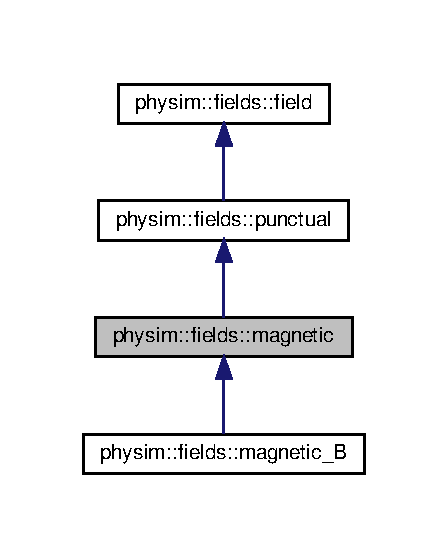
\includegraphics[width=215pt]{classphysim_1_1fields_1_1magnetic__inherit__graph}
\end{center}
\end{figure}


Collaboration diagram for physim\+:\+:fields\+:\+:magnetic\+:\nopagebreak
\begin{figure}[H]
\begin{center}
\leavevmode
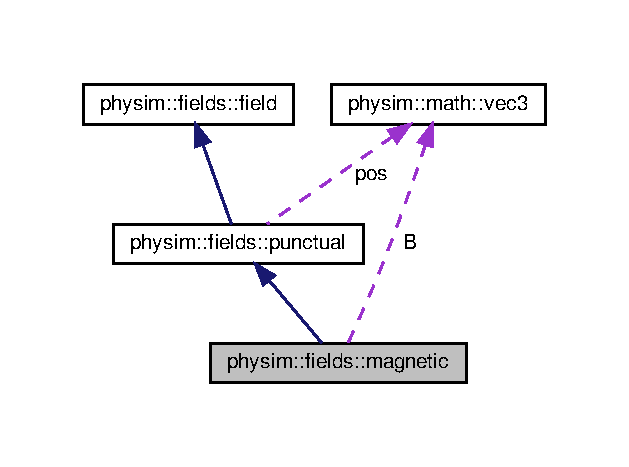
\includegraphics[width=302pt]{classphysim_1_1fields_1_1magnetic__coll__graph}
\end{center}
\end{figure}
\subsection*{Public Member Functions}
\begin{DoxyCompactItemize}
\item 
\hyperlink{classphysim_1_1fields_1_1magnetic_a4bc1ebfece31aa73f3242850314dcaac}{magnetic} ()
\begin{DoxyCompactList}\small\item\em Default constructor. \end{DoxyCompactList}\item 
\mbox{\Hypertarget{classphysim_1_1fields_1_1magnetic_ae7e5039ac9ffa0e4283698c6215ae8cf}\label{classphysim_1_1fields_1_1magnetic_ae7e5039ac9ffa0e4283698c6215ae8cf}} 
\hyperlink{classphysim_1_1fields_1_1magnetic_ae7e5039ac9ffa0e4283698c6215ae8cf}{magnetic} (const \hyperlink{structphysim_1_1math_1_1vec3}{math\+::vec3} \&\hyperlink{classphysim_1_1fields_1_1punctual_a00344d6f3e4f3f841e7d876918c66977}{pos}, const \hyperlink{structphysim_1_1math_1_1vec3}{math\+::vec3} \&b)
\begin{DoxyCompactList}\small\item\em Constructor with magnetic field vector. \end{DoxyCompactList}\item 
\mbox{\Hypertarget{classphysim_1_1fields_1_1magnetic_a573c07a7a049bebe1f47eef6621cc2cd}\label{classphysim_1_1fields_1_1magnetic_a573c07a7a049bebe1f47eef6621cc2cd}} 
\hyperlink{classphysim_1_1fields_1_1magnetic_a573c07a7a049bebe1f47eef6621cc2cd}{magnetic} (const \hyperlink{classphysim_1_1fields_1_1magnetic}{magnetic} \&f)
\begin{DoxyCompactList}\small\item\em Copy constructor. \end{DoxyCompactList}\item 
\mbox{\Hypertarget{classphysim_1_1fields_1_1magnetic_a8263839cd27980407f2480601e677f4a}\label{classphysim_1_1fields_1_1magnetic_a8263839cd27980407f2480601e677f4a}} 
virtual \hyperlink{classphysim_1_1fields_1_1magnetic_a8263839cd27980407f2480601e677f4a}{$\sim$magnetic} ()
\begin{DoxyCompactList}\small\item\em Destructor. \end{DoxyCompactList}\item 
\mbox{\Hypertarget{classphysim_1_1fields_1_1magnetic_a405a791a9e5a711eb6a43de73462c609}\label{classphysim_1_1fields_1_1magnetic_a405a791a9e5a711eb6a43de73462c609}} 
void \hyperlink{classphysim_1_1fields_1_1magnetic_a405a791a9e5a711eb6a43de73462c609}{set\+\_\+vector} (const \hyperlink{structphysim_1_1math_1_1vec3}{math\+::vec3} \&v)
\begin{DoxyCompactList}\small\item\em Sets this magnetic field vector. See \hyperlink{classphysim_1_1fields_1_1magnetic_a9955f0d4a3773ff96b536f37623b5ac7}{B}. \end{DoxyCompactList}\item 
\mbox{\Hypertarget{classphysim_1_1fields_1_1magnetic_a279376a78adda4e96bc02aef38cb54bd}\label{classphysim_1_1fields_1_1magnetic_a279376a78adda4e96bc02aef38cb54bd}} 
const \hyperlink{structphysim_1_1math_1_1vec3}{math\+::vec3} \& \hyperlink{classphysim_1_1fields_1_1magnetic_a279376a78adda4e96bc02aef38cb54bd}{get\+\_\+vector} () const
\begin{DoxyCompactList}\small\item\em Returns this field\textquotesingle{}s magnetic vector. See \hyperlink{classphysim_1_1fields_1_1magnetic_a9955f0d4a3773ff96b536f37623b5ac7}{B}. \end{DoxyCompactList}\end{DoxyCompactItemize}
\subsection*{Protected Attributes}
\begin{DoxyCompactItemize}
\item 
\mbox{\Hypertarget{classphysim_1_1fields_1_1magnetic_a9955f0d4a3773ff96b536f37623b5ac7}\label{classphysim_1_1fields_1_1magnetic_a9955f0d4a3773ff96b536f37623b5ac7}} 
\hyperlink{structphysim_1_1math_1_1vec3}{math\+::vec3} \hyperlink{classphysim_1_1fields_1_1magnetic_a9955f0d4a3773ff96b536f37623b5ac7}{B}
\begin{DoxyCompactList}\small\item\em Magnetic field vector \mbox{[}T\mbox{]}. \end{DoxyCompactList}\end{DoxyCompactItemize}


\subsection{Detailed Description}
Punctual magnetic field. 

Described by a position \hyperlink{classphysim_1_1fields_1_1punctual_a00344d6f3e4f3f841e7d876918c66977}{pos} and a magentic field vector \hyperlink{classphysim_1_1fields_1_1magnetic_a9955f0d4a3773ff96b536f37623b5ac7}{B}.

There are several types of magnetic fields. As an example, see \hyperlink{classphysim_1_1fields_1_1magnetic__B}{magnetic\+\_\+B}. 

\subsection{Constructor \& Destructor Documentation}
\mbox{\Hypertarget{classphysim_1_1fields_1_1magnetic_a4bc1ebfece31aa73f3242850314dcaac}\label{classphysim_1_1fields_1_1magnetic_a4bc1ebfece31aa73f3242850314dcaac}} 
\index{physim\+::fields\+::magnetic@{physim\+::fields\+::magnetic}!magnetic@{magnetic}}
\index{magnetic@{magnetic}!physim\+::fields\+::magnetic@{physim\+::fields\+::magnetic}}
\subsubsection{\texorpdfstring{magnetic()}{magnetic()}}
{\footnotesize\ttfamily physim\+::fields\+::magnetic\+::magnetic (\begin{DoxyParamCaption}{ }\end{DoxyParamCaption})}



Default constructor. 

The magnetic field vector \hyperlink{classphysim_1_1fields_1_1magnetic_a9955f0d4a3773ff96b536f37623b5ac7}{B} is initialised to (0,0,0). 

The documentation for this class was generated from the following files\+:\begin{DoxyCompactItemize}
\item 
physim/fields/magnetic.\+hpp\item 
physim/fields/magnetic.\+cpp\end{DoxyCompactItemize}

\hypertarget{classphysim_1_1fields_1_1magnetic__B}{}\section{physim\+:\+:fields\+:\+:magnetic\+\_\+B Class Reference}
\label{classphysim_1_1fields_1_1magnetic__B}\index{physim\+::fields\+::magnetic\+\_\+B@{physim\+::fields\+::magnetic\+\_\+B}}


Implementation of a magnetic B-\/field.  




{\ttfamily \#include $<$magnetic\+\_\+\+B.\+hpp$>$}



Inheritance diagram for physim\+:\+:fields\+:\+:magnetic\+\_\+B\+:\nopagebreak
\begin{figure}[H]
\begin{center}
\leavevmode
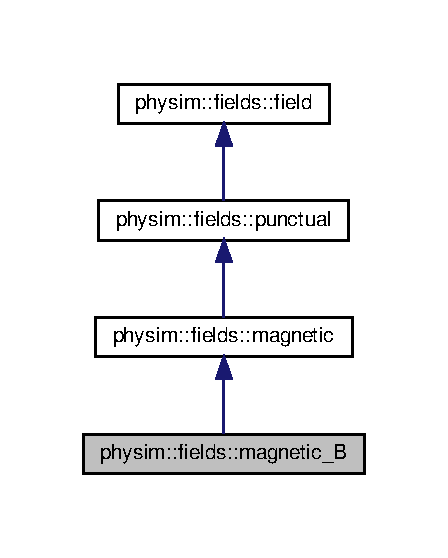
\includegraphics[width=215pt]{classphysim_1_1fields_1_1magnetic__B__inherit__graph}
\end{center}
\end{figure}


Collaboration diagram for physim\+:\+:fields\+:\+:magnetic\+\_\+B\+:\nopagebreak
\begin{figure}[H]
\begin{center}
\leavevmode
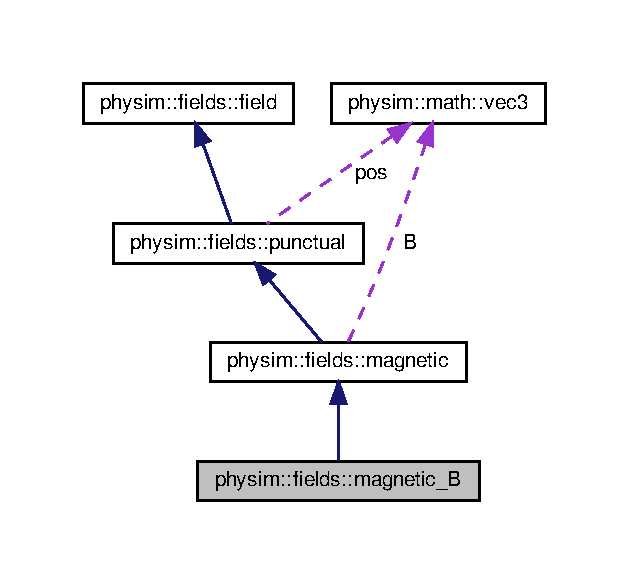
\includegraphics[width=302pt]{classphysim_1_1fields_1_1magnetic__B__coll__graph}
\end{center}
\end{figure}
\subsection*{Public Member Functions}
\begin{DoxyCompactItemize}
\item 
\mbox{\Hypertarget{classphysim_1_1fields_1_1magnetic__B_ab5da6ab1de8e9724f61cad63fe21f374}\label{classphysim_1_1fields_1_1magnetic__B_ab5da6ab1de8e9724f61cad63fe21f374}} 
\hyperlink{classphysim_1_1fields_1_1magnetic__B_ab5da6ab1de8e9724f61cad63fe21f374}{magnetic\+\_\+B} ()
\begin{DoxyCompactList}\small\item\em Default constructor. \end{DoxyCompactList}\item 
\mbox{\Hypertarget{classphysim_1_1fields_1_1magnetic__B_a5541b899c3f02a42b0aa67f4ec18c824}\label{classphysim_1_1fields_1_1magnetic__B_a5541b899c3f02a42b0aa67f4ec18c824}} 
\hyperlink{classphysim_1_1fields_1_1magnetic__B_a5541b899c3f02a42b0aa67f4ec18c824}{magnetic\+\_\+B} (const \hyperlink{structphysim_1_1math_1_1vec3}{math\+::vec3} \&\hyperlink{classphysim_1_1fields_1_1punctual_a00344d6f3e4f3f841e7d876918c66977}{pos}, const \hyperlink{structphysim_1_1math_1_1vec3}{math\+::vec3} \&b)
\begin{DoxyCompactList}\small\item\em Constructor with position and magnetic field vector. \end{DoxyCompactList}\item 
\mbox{\Hypertarget{classphysim_1_1fields_1_1magnetic__B_ada69a69a5582e244210f10d8d1e69426}\label{classphysim_1_1fields_1_1magnetic__B_ada69a69a5582e244210f10d8d1e69426}} 
\hyperlink{classphysim_1_1fields_1_1magnetic__B_ada69a69a5582e244210f10d8d1e69426}{magnetic\+\_\+B} (const \hyperlink{classphysim_1_1fields_1_1magnetic__B}{magnetic\+\_\+B} \&f)
\begin{DoxyCompactList}\small\item\em Copy constructor. \end{DoxyCompactList}\item 
\mbox{\Hypertarget{classphysim_1_1fields_1_1magnetic__B_ab6e422ab8c678c67e447db13742f1180}\label{classphysim_1_1fields_1_1magnetic__B_ab6e422ab8c678c67e447db13742f1180}} 
virtual \hyperlink{classphysim_1_1fields_1_1magnetic__B_ab6e422ab8c678c67e447db13742f1180}{$\sim$magnetic\+\_\+B} ()
\begin{DoxyCompactList}\small\item\em Destructor. \end{DoxyCompactList}\item 
void \hyperlink{classphysim_1_1fields_1_1magnetic__B_a806a3e8aa306f0ed33954d79c3082698}{compute\+\_\+force} (const \hyperlink{classphysim_1_1particles_1_1free__particle}{particles\+::free\+\_\+particle} \&p, \hyperlink{structphysim_1_1math_1_1vec3}{math\+::vec3} \&F)
\begin{DoxyCompactList}\small\item\em Compute the force vector acting on a particle. \end{DoxyCompactList}\item 
void \hyperlink{classphysim_1_1fields_1_1magnetic__B_aa337b83c6dea0726d2dc2d7cd1cd978a}{compute\+\_\+force} (const \hyperlink{classphysim_1_1particles_1_1mesh__particle}{particles\+::mesh\+\_\+particle} \&p, \hyperlink{structphysim_1_1math_1_1vec3}{math\+::vec3} \&F)
\begin{DoxyCompactList}\small\item\em Compute the force vector acting on a particle. \end{DoxyCompactList}\item 
void \hyperlink{classphysim_1_1fields_1_1magnetic__B_a17ca2b3c6cbf61c53665cf23632187b8}{compute\+\_\+force} (const \hyperlink{classphysim_1_1particles_1_1fluid__particle}{particles\+::fluid\+\_\+particle} \&p, \hyperlink{structphysim_1_1math_1_1vec3}{math\+::vec3} \&F)
\begin{DoxyCompactList}\small\item\em Compute the force vector acting on a particle. \end{DoxyCompactList}\end{DoxyCompactItemize}
\subsection*{Private Member Functions}
\begin{DoxyCompactItemize}
\item 
{\footnotesize template$<$class P $>$ }\\void \hyperlink{classphysim_1_1fields_1_1magnetic__B_ad7c54b149a9a43b086dfab580129bfb2}{\+\_\+\+\_\+compute\+\_\+force} (const P \&p, \hyperlink{structphysim_1_1math_1_1vec3}{math\+::vec3} \&F)
\begin{DoxyCompactList}\small\item\em Function that actuall computes the force of this field. \end{DoxyCompactList}\end{DoxyCompactItemize}
\subsection*{Additional Inherited Members}


\subsection{Detailed Description}
Implementation of a magnetic B-\/field. 

The force that acts on a particle is calculated as\+:

$ \vec{F} = (q \cdot v_p) \times \vec{B}$, where $q$ is the charge of the particle (see \hyperlink{classphysim_1_1particles_1_1free__particle_a7513ac41f3cab1ce083f8695e2c73301}{free\+\_\+particle\+::charge} and \hyperlink{classphysim_1_1particles_1_1mesh__particle_adf14d64e9effa2bcf5cb84a537bd8027}{mesh\+\_\+particle\+::charge}), $B$ is the magnetic field vector (see \hyperlink{classphysim_1_1fields_1_1magnetic_a9955f0d4a3773ff96b536f37623b5ac7}{magnetic\+::B}) and $v_p$ is the particle\textquotesingle{}s punctual velocity (see \hyperlink{classphysim_1_1particles_1_1base__particle_a66a164d2a130c40901e3ec2709cdad43}{free\+\_\+particle\+::cur\+\_\+vel} and see \hyperlink{classphysim_1_1particles_1_1base__particle_a66a164d2a130c40901e3ec2709cdad43}{mesh\+\_\+particle\+::cur\+\_\+vel}). 

\subsection{Member Function Documentation}
\mbox{\Hypertarget{classphysim_1_1fields_1_1magnetic__B_ad7c54b149a9a43b086dfab580129bfb2}\label{classphysim_1_1fields_1_1magnetic__B_ad7c54b149a9a43b086dfab580129bfb2}} 
\index{physim\+::fields\+::magnetic\+\_\+B@{physim\+::fields\+::magnetic\+\_\+B}!\+\_\+\+\_\+compute\+\_\+force@{\+\_\+\+\_\+compute\+\_\+force}}
\index{\+\_\+\+\_\+compute\+\_\+force@{\+\_\+\+\_\+compute\+\_\+force}!physim\+::fields\+::magnetic\+\_\+B@{physim\+::fields\+::magnetic\+\_\+B}}
\subsubsection{\texorpdfstring{\+\_\+\+\_\+compute\+\_\+force()}{\_\_compute\_force()}}
{\footnotesize\ttfamily template$<$class P $>$ \\
void physim\+::fields\+::magnetic\+\_\+\+B\+::\+\_\+\+\_\+compute\+\_\+force (\begin{DoxyParamCaption}\item[{const P \&}]{p,  }\item[{\hyperlink{structphysim_1_1math_1_1vec3}{math\+::vec3} \&}]{F }\end{DoxyParamCaption})\hspace{0.3cm}{\ttfamily [private]}}



Function that actuall computes the force of this field. 

Works for \hyperlink{classphysim_1_1particles_1_1free__particle}{particles\+::free\+\_\+particle} and \hyperlink{classphysim_1_1particles_1_1mesh__particle}{particles\+::mesh\+\_\+particle}. \mbox{\Hypertarget{classphysim_1_1fields_1_1magnetic__B_a806a3e8aa306f0ed33954d79c3082698}\label{classphysim_1_1fields_1_1magnetic__B_a806a3e8aa306f0ed33954d79c3082698}} 
\index{physim\+::fields\+::magnetic\+\_\+B@{physim\+::fields\+::magnetic\+\_\+B}!compute\+\_\+force@{compute\+\_\+force}}
\index{compute\+\_\+force@{compute\+\_\+force}!physim\+::fields\+::magnetic\+\_\+B@{physim\+::fields\+::magnetic\+\_\+B}}
\subsubsection{\texorpdfstring{compute\+\_\+force()}{compute\_force()}\hspace{0.1cm}{\footnotesize\ttfamily [1/3]}}
{\footnotesize\ttfamily void physim\+::fields\+::magnetic\+\_\+\+B\+::compute\+\_\+force (\begin{DoxyParamCaption}\item[{const \hyperlink{classphysim_1_1particles_1_1free__particle}{particles\+::free\+\_\+particle} \&}]{p,  }\item[{\hyperlink{structphysim_1_1math_1_1vec3}{math\+::vec3} \&}]{F }\end{DoxyParamCaption})\hspace{0.3cm}{\ttfamily [virtual]}}



Compute the force vector acting on a particle. 

The contents of parameter {\itshape F} is undefined when calling this function, thus the contents should be overwritten. 
\begin{DoxyParams}[1]{Parameters}
\mbox{\tt in}  & {\em p} & Particle where the force is applied to. \\
\hline
\mbox{\tt out}  & {\em F} & The force from this field acting on the particle. \\
\hline
\end{DoxyParams}


Implements \hyperlink{classphysim_1_1fields_1_1field_a0d836756ac51a6a1e99d3c9a60310694}{physim\+::fields\+::field}.

\mbox{\Hypertarget{classphysim_1_1fields_1_1magnetic__B_aa337b83c6dea0726d2dc2d7cd1cd978a}\label{classphysim_1_1fields_1_1magnetic__B_aa337b83c6dea0726d2dc2d7cd1cd978a}} 
\index{physim\+::fields\+::magnetic\+\_\+B@{physim\+::fields\+::magnetic\+\_\+B}!compute\+\_\+force@{compute\+\_\+force}}
\index{compute\+\_\+force@{compute\+\_\+force}!physim\+::fields\+::magnetic\+\_\+B@{physim\+::fields\+::magnetic\+\_\+B}}
\subsubsection{\texorpdfstring{compute\+\_\+force()}{compute\_force()}\hspace{0.1cm}{\footnotesize\ttfamily [2/3]}}
{\footnotesize\ttfamily void physim\+::fields\+::magnetic\+\_\+\+B\+::compute\+\_\+force (\begin{DoxyParamCaption}\item[{const \hyperlink{classphysim_1_1particles_1_1mesh__particle}{particles\+::mesh\+\_\+particle} \&}]{p,  }\item[{\hyperlink{structphysim_1_1math_1_1vec3}{math\+::vec3} \&}]{F }\end{DoxyParamCaption})\hspace{0.3cm}{\ttfamily [virtual]}}



Compute the force vector acting on a particle. 

The contents of parameter {\itshape F} is undefined when calling this function, thus the contents should be overwritten. 
\begin{DoxyParams}[1]{Parameters}
\mbox{\tt in}  & {\em p} & Particle where the force is applied to. \\
\hline
\mbox{\tt out}  & {\em F} & The force from this field acting on the particle. \\
\hline
\end{DoxyParams}


Implements \hyperlink{classphysim_1_1fields_1_1field_aa167d81f223daab47989168c9d3b8cb4}{physim\+::fields\+::field}.

\mbox{\Hypertarget{classphysim_1_1fields_1_1magnetic__B_a17ca2b3c6cbf61c53665cf23632187b8}\label{classphysim_1_1fields_1_1magnetic__B_a17ca2b3c6cbf61c53665cf23632187b8}} 
\index{physim\+::fields\+::magnetic\+\_\+B@{physim\+::fields\+::magnetic\+\_\+B}!compute\+\_\+force@{compute\+\_\+force}}
\index{compute\+\_\+force@{compute\+\_\+force}!physim\+::fields\+::magnetic\+\_\+B@{physim\+::fields\+::magnetic\+\_\+B}}
\subsubsection{\texorpdfstring{compute\+\_\+force()}{compute\_force()}\hspace{0.1cm}{\footnotesize\ttfamily [3/3]}}
{\footnotesize\ttfamily void physim\+::fields\+::magnetic\+\_\+\+B\+::compute\+\_\+force (\begin{DoxyParamCaption}\item[{const \hyperlink{classphysim_1_1particles_1_1fluid__particle}{particles\+::fluid\+\_\+particle} \&}]{p,  }\item[{\hyperlink{structphysim_1_1math_1_1vec3}{math\+::vec3} \&}]{F }\end{DoxyParamCaption})\hspace{0.3cm}{\ttfamily [virtual]}}



Compute the force vector acting on a particle. 

The contents of parameter {\itshape F} is undefined when calling this function, thus the contents should be overwritten. 
\begin{DoxyParams}[1]{Parameters}
\mbox{\tt in}  & {\em p} & Particle where the force is applied to. \\
\hline
\mbox{\tt out}  & {\em F} & The force from this field acting on the particle. \\
\hline
\end{DoxyParams}


Implements \hyperlink{classphysim_1_1fields_1_1field_a099fb8b1dee7afae4610c6275432bc81}{physim\+::fields\+::field}.



The documentation for this class was generated from the following files\+:\begin{DoxyCompactItemize}
\item 
physim/fields/magnetic\+\_\+\+B.\+hpp\item 
physim/fields/magnetic\+\_\+\+B.\+cpp\end{DoxyCompactItemize}

\hypertarget{classphysim_1_1meshes_1_1mesh}{}\section{physim\+:\+:meshes\+:\+:mesh Class Reference}
\label{classphysim_1_1meshes_1_1mesh}\index{physim\+::meshes\+::mesh@{physim\+::meshes\+::mesh}}


Abstract spring mesh.  




{\ttfamily \#include $<$mesh.\+hpp$>$}



Inheritance diagram for physim\+:\+:meshes\+:\+:mesh\+:\nopagebreak
\begin{figure}[H]
\begin{center}
\leavevmode
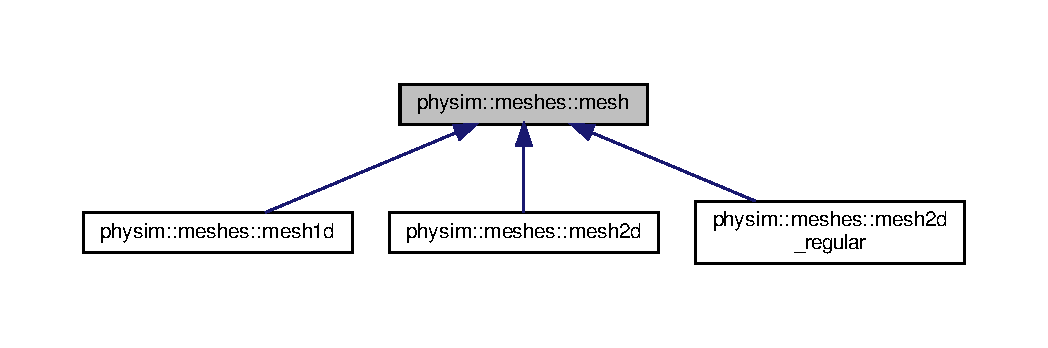
\includegraphics[width=350pt]{classphysim_1_1meshes_1_1mesh__inherit__graph}
\end{center}
\end{figure}


Collaboration diagram for physim\+:\+:meshes\+:\+:mesh\+:\nopagebreak
\begin{figure}[H]
\begin{center}
\leavevmode
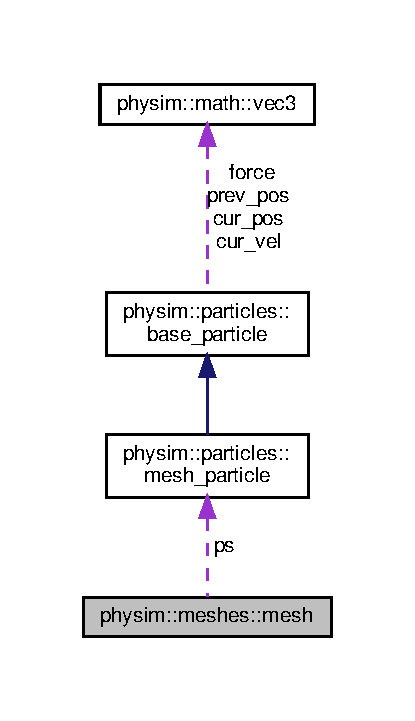
\includegraphics[width=199pt]{classphysim_1_1meshes_1_1mesh__coll__graph}
\end{center}
\end{figure}
\subsection*{Public Member Functions}
\begin{DoxyCompactItemize}
\item 
\mbox{\Hypertarget{classphysim_1_1meshes_1_1mesh_a923bdaeba6dff1d95c2e55a80bfb26b5}\label{classphysim_1_1meshes_1_1mesh_a923bdaeba6dff1d95c2e55a80bfb26b5}} 
\hyperlink{classphysim_1_1meshes_1_1mesh_a923bdaeba6dff1d95c2e55a80bfb26b5}{mesh} ()
\begin{DoxyCompactList}\small\item\em Default constructor. \end{DoxyCompactList}\item 
\hyperlink{classphysim_1_1meshes_1_1mesh_a853728b532513cf9fe5f0df25f88358f}{mesh} (float ke, float kd)
\begin{DoxyCompactList}\small\item\em Constructor with parameters. \end{DoxyCompactList}\item 
virtual \hyperlink{classphysim_1_1meshes_1_1mesh_a51250a9f06eabd7cf05c0af7c3d7138c}{$\sim$mesh} ()
\begin{DoxyCompactList}\small\item\em Destructor. \end{DoxyCompactList}\item 
\mbox{\Hypertarget{classphysim_1_1meshes_1_1mesh_ae238482532e415ee3585765db2427731}\label{classphysim_1_1meshes_1_1mesh_ae238482532e415ee3585765db2427731}} 
\hyperlink{classphysim_1_1particles_1_1mesh__particle}{particles\+::mesh\+\_\+particle} \& \hyperlink{classphysim_1_1meshes_1_1mesh_ae238482532e415ee3585765db2427731}{operator\mbox{[}$\,$\mbox{]}} (size\+\_\+t i)
\begin{DoxyCompactList}\small\item\em Returns a reference to the {\itshape i-\/th} particle. \end{DoxyCompactList}\item 
\mbox{\Hypertarget{classphysim_1_1meshes_1_1mesh_a37064be55680e2ae0b30fd3fe8cd5816}\label{classphysim_1_1meshes_1_1mesh_a37064be55680e2ae0b30fd3fe8cd5816}} 
const \hyperlink{classphysim_1_1particles_1_1mesh__particle}{particles\+::mesh\+\_\+particle} \& \hyperlink{classphysim_1_1meshes_1_1mesh_a37064be55680e2ae0b30fd3fe8cd5816}{operator\mbox{[}$\,$\mbox{]}} (size\+\_\+t i) const
\begin{DoxyCompactList}\small\item\em Returns a constant reference to the {\itshape i-\/th} particle. \end{DoxyCompactList}\item 
void \hyperlink{classphysim_1_1meshes_1_1mesh_a09dcfcda6da092c7acae3f961fde4b32}{allocate} (size\+\_\+t n, float Kg=1.\+0f)
\begin{DoxyCompactList}\small\item\em Allocates memory for {\itshape n} particles. \end{DoxyCompactList}\item 
\mbox{\Hypertarget{classphysim_1_1meshes_1_1mesh_ae2923846bfeec345fae4876181960c03}\label{classphysim_1_1meshes_1_1mesh_ae2923846bfeec345fae4876181960c03}} 
virtual void \hyperlink{classphysim_1_1meshes_1_1mesh_ae2923846bfeec345fae4876181960c03}{clear} ()
\begin{DoxyCompactList}\small\item\em Frees the memory occupied by this mesh. \end{DoxyCompactList}\item 
virtual void \hyperlink{classphysim_1_1meshes_1_1mesh_a62f877dd42bc306ef70c76fc172f245f}{make\+\_\+initial\+\_\+state} ()=0
\begin{DoxyCompactList}\small\item\em Builds the initial state of the mesh. \end{DoxyCompactList}\item 
virtual void \hyperlink{classphysim_1_1meshes_1_1mesh_ad7cad4cd454cce562c8c404ef09f8bd3}{update\+\_\+forces} ()=0
\begin{DoxyCompactList}\small\item\em Update the forces generated within the mesh. \end{DoxyCompactList}\item 
\mbox{\Hypertarget{classphysim_1_1meshes_1_1mesh_a1b12b241f860fea09d17196132cf46da}\label{classphysim_1_1meshes_1_1mesh_a1b12b241f860fea09d17196132cf46da}} 
void \hyperlink{classphysim_1_1meshes_1_1mesh_a1b12b241f860fea09d17196132cf46da}{set\+\_\+elasticity} (float ke)
\begin{DoxyCompactList}\small\item\em Sets the elasticity coefficient of this mesh. \end{DoxyCompactList}\item 
\mbox{\Hypertarget{classphysim_1_1meshes_1_1mesh_a54b38e38d22ba1e4b4966c29e0fcb3ea}\label{classphysim_1_1meshes_1_1mesh_a54b38e38d22ba1e4b4966c29e0fcb3ea}} 
void \hyperlink{classphysim_1_1meshes_1_1mesh_a54b38e38d22ba1e4b4966c29e0fcb3ea}{set\+\_\+damping} (float kd)
\begin{DoxyCompactList}\small\item\em Sets the damping factor of this mesh. \end{DoxyCompactList}\item 
\mbox{\Hypertarget{classphysim_1_1meshes_1_1mesh_a8933b7d34f1b92f0348d2d7223ad747f}\label{classphysim_1_1meshes_1_1mesh_a8933b7d34f1b92f0348d2d7223ad747f}} 
void \hyperlink{classphysim_1_1meshes_1_1mesh_a8933b7d34f1b92f0348d2d7223ad747f}{set\+\_\+friction} (float ke)
\begin{DoxyCompactList}\small\item\em Sets the friction coefficient of this mesh. \end{DoxyCompactList}\item 
\mbox{\Hypertarget{classphysim_1_1meshes_1_1mesh_a729ee4377e1d4159ac5844b014521b88}\label{classphysim_1_1meshes_1_1mesh_a729ee4377e1d4159ac5844b014521b88}} 
void \hyperlink{classphysim_1_1meshes_1_1mesh_a729ee4377e1d4159ac5844b014521b88}{set\+\_\+bouncing} (float kd)
\begin{DoxyCompactList}\small\item\em Sets the bouncing factor of this mesh. \end{DoxyCompactList}\item 
void \hyperlink{classphysim_1_1meshes_1_1mesh_a8eabfe8ed4457f150a1f401ac116a3de}{set\+\_\+mass} (float Kg)
\begin{DoxyCompactList}\small\item\em Sets the mass (in Kg) of the mesh. \end{DoxyCompactList}\item 
\mbox{\Hypertarget{classphysim_1_1meshes_1_1mesh_a683ae48a5d7468d081d971835522813a}\label{classphysim_1_1meshes_1_1mesh_a683ae48a5d7468d081d971835522813a}} 
float \hyperlink{classphysim_1_1meshes_1_1mesh_a683ae48a5d7468d081d971835522813a}{get\+\_\+elasticity} () const
\begin{DoxyCompactList}\small\item\em Returns the elasticity coefficient of this mesh. \end{DoxyCompactList}\item 
\mbox{\Hypertarget{classphysim_1_1meshes_1_1mesh_a861b09b83121d7d7f025abd6c1719b01}\label{classphysim_1_1meshes_1_1mesh_a861b09b83121d7d7f025abd6c1719b01}} 
float \hyperlink{classphysim_1_1meshes_1_1mesh_a861b09b83121d7d7f025abd6c1719b01}{get\+\_\+damping} () const
\begin{DoxyCompactList}\small\item\em Returns the damping factor of this mesh. \end{DoxyCompactList}\item 
\mbox{\Hypertarget{classphysim_1_1meshes_1_1mesh_a40c01dbcea91b285437dceed1246a5ce}\label{classphysim_1_1meshes_1_1mesh_a40c01dbcea91b285437dceed1246a5ce}} 
float \hyperlink{classphysim_1_1meshes_1_1mesh_a40c01dbcea91b285437dceed1246a5ce}{get\+\_\+friction} () const
\begin{DoxyCompactList}\small\item\em Returns the friction coefficient of this mesh. \end{DoxyCompactList}\item 
\mbox{\Hypertarget{classphysim_1_1meshes_1_1mesh_a95b803bd21567fe3d3f9507a92e0357c}\label{classphysim_1_1meshes_1_1mesh_a95b803bd21567fe3d3f9507a92e0357c}} 
float \hyperlink{classphysim_1_1meshes_1_1mesh_a95b803bd21567fe3d3f9507a92e0357c}{get\+\_\+bouncing} () const
\begin{DoxyCompactList}\small\item\em Returns the bouncing factor of this mesh. \end{DoxyCompactList}\item 
\mbox{\Hypertarget{classphysim_1_1meshes_1_1mesh_aac74989eef79d2cbc342d276f4215872}\label{classphysim_1_1meshes_1_1mesh_aac74989eef79d2cbc342d276f4215872}} 
size\+\_\+t \hyperlink{classphysim_1_1meshes_1_1mesh_aac74989eef79d2cbc342d276f4215872}{size} () const
\begin{DoxyCompactList}\small\item\em Returns the number of particles of this mesh. \end{DoxyCompactList}\item 
\mbox{\Hypertarget{classphysim_1_1meshes_1_1mesh_a016d53d761ee8b9b5121b347f071ff6a}\label{classphysim_1_1meshes_1_1mesh_a016d53d761ee8b9b5121b347f071ff6a}} 
const \hyperlink{namespacephysim_1_1meshes_a0a3501674fecdbcbbee92c4c3bb68a67}{mesh\+\_\+type} \& \hyperlink{classphysim_1_1meshes_1_1mesh_a016d53d761ee8b9b5121b347f071ff6a}{get\+\_\+type} () const
\begin{DoxyCompactList}\small\item\em Returns the type of this mesh. See \hyperlink{classphysim_1_1meshes_1_1mesh_a0775ba21bb034b19e9ce1314f9a3b995}{mt}. \end{DoxyCompactList}\item 
\mbox{\Hypertarget{classphysim_1_1meshes_1_1mesh_ad1a34e0170bf12b81d9b04d75f0737e2}\label{classphysim_1_1meshes_1_1mesh_ad1a34e0170bf12b81d9b04d75f0737e2}} 
\hyperlink{classphysim_1_1particles_1_1mesh__particle}{particles\+::mesh\+\_\+particle} $\ast$ \hyperlink{classphysim_1_1meshes_1_1mesh_ad1a34e0170bf12b81d9b04d75f0737e2}{get\+\_\+particles} ()
\begin{DoxyCompactList}\small\item\em Returns a reference to this mesh\textquotesingle{}s particles. \end{DoxyCompactList}\item 
\mbox{\Hypertarget{classphysim_1_1meshes_1_1mesh_a689c4b1ea0b9522dd8e9564c7bbacdd2}\label{classphysim_1_1meshes_1_1mesh_a689c4b1ea0b9522dd8e9564c7bbacdd2}} 
const \hyperlink{classphysim_1_1particles_1_1mesh__particle}{particles\+::mesh\+\_\+particle} $\ast$ \hyperlink{classphysim_1_1meshes_1_1mesh_a689c4b1ea0b9522dd8e9564c7bbacdd2}{get\+\_\+particles} () const
\begin{DoxyCompactList}\small\item\em Returns a constant reference to this mesh\textquotesingle{}s particles. \end{DoxyCompactList}\end{DoxyCompactItemize}
\subsection*{Protected Attributes}
\begin{DoxyCompactItemize}
\item 
\mbox{\Hypertarget{classphysim_1_1meshes_1_1mesh_a0775ba21bb034b19e9ce1314f9a3b995}\label{classphysim_1_1meshes_1_1mesh_a0775ba21bb034b19e9ce1314f9a3b995}} 
\hyperlink{namespacephysim_1_1meshes_a0a3501674fecdbcbbee92c4c3bb68a67}{mesh\+\_\+type} \hyperlink{classphysim_1_1meshes_1_1mesh_a0775ba21bb034b19e9ce1314f9a3b995}{mt}
\begin{DoxyCompactList}\small\item\em The type of this mesh. \end{DoxyCompactList}\item 
\mbox{\Hypertarget{classphysim_1_1meshes_1_1mesh_a5642217313d7dae9f873f01fad682ff2}\label{classphysim_1_1meshes_1_1mesh_a5642217313d7dae9f873f01fad682ff2}} 
size\+\_\+t \hyperlink{classphysim_1_1meshes_1_1mesh_a5642217313d7dae9f873f01fad682ff2}{N}
\begin{DoxyCompactList}\small\item\em Total number of particles of the mesh. \end{DoxyCompactList}\item 
\mbox{\Hypertarget{classphysim_1_1meshes_1_1mesh_adb7eb9def630cc025997f859c74afd58}\label{classphysim_1_1meshes_1_1mesh_adb7eb9def630cc025997f859c74afd58}} 
\hyperlink{classphysim_1_1particles_1_1mesh__particle}{particles\+::mesh\+\_\+particle} $\ast$ \hyperlink{classphysim_1_1meshes_1_1mesh_adb7eb9def630cc025997f859c74afd58}{ps}
\begin{DoxyCompactList}\small\item\em The particles of this mesh. \end{DoxyCompactList}\item 
\mbox{\Hypertarget{classphysim_1_1meshes_1_1mesh_ab5afc13f5931c6a9df16d5ee49edc453}\label{classphysim_1_1meshes_1_1mesh_ab5afc13f5931c6a9df16d5ee49edc453}} 
float \hyperlink{classphysim_1_1meshes_1_1mesh_ab5afc13f5931c6a9df16d5ee49edc453}{Ke}
\begin{DoxyCompactList}\small\item\em Elasticity coefficient of each spring. \end{DoxyCompactList}\item 
\mbox{\Hypertarget{classphysim_1_1meshes_1_1mesh_abba546f70a90e7678efc5b746cf1ccd1}\label{classphysim_1_1meshes_1_1mesh_abba546f70a90e7678efc5b746cf1ccd1}} 
float \hyperlink{classphysim_1_1meshes_1_1mesh_abba546f70a90e7678efc5b746cf1ccd1}{Kd}
\begin{DoxyCompactList}\small\item\em Damping factor of each spring. \end{DoxyCompactList}\item 
\mbox{\Hypertarget{classphysim_1_1meshes_1_1mesh_a90dc28ae4b66272d40615cb55596383a}\label{classphysim_1_1meshes_1_1mesh_a90dc28ae4b66272d40615cb55596383a}} 
float \hyperlink{classphysim_1_1meshes_1_1mesh_a90dc28ae4b66272d40615cb55596383a}{bouncing}
\begin{DoxyCompactList}\small\item\em Bouncing coefficient of all the particles in the mesh. \end{DoxyCompactList}\item 
\mbox{\Hypertarget{classphysim_1_1meshes_1_1mesh_a131fe4688049ea2ec62ef108aee1944c}\label{classphysim_1_1meshes_1_1mesh_a131fe4688049ea2ec62ef108aee1944c}} 
float \hyperlink{classphysim_1_1meshes_1_1mesh_a131fe4688049ea2ec62ef108aee1944c}{friction}
\begin{DoxyCompactList}\small\item\em Friction coefficient of all the particles in the mesh. \end{DoxyCompactList}\end{DoxyCompactItemize}


\subsection{Detailed Description}
Abstract spring mesh. 

This represents a set of \hyperlink{classphysim_1_1particles_1_1mesh__particle}{particles\+::mesh\+\_\+particle} where one particle is attached to some other particles of the same mesh with a spring. The movement of one particle in the spring, then, affects the other particles it is attached to. Each particle has a local index {\itshape i} that ranges between 0 and the number of particles -\/ 1.

All the springs of the mesh are described similarly with the following coefficients\+:
\begin{DoxyItemize}
\item elasticity parameter (see \hyperlink{classphysim_1_1meshes_1_1mesh_ab5afc13f5931c6a9df16d5ee49edc453}{Ke}).
\item damping factor (see \hyperlink{classphysim_1_1meshes_1_1mesh_abba546f70a90e7678efc5b746cf1ccd1}{Kd}).
\end{DoxyItemize}

Some coefficients are common to all the particles\+:
\begin{DoxyItemize}
\item bouncing coefficient (see \hyperlink{classphysim_1_1meshes_1_1mesh_a90dc28ae4b66272d40615cb55596383a}{bouncing}).
\item friction coefficient (see \hyperlink{classphysim_1_1meshes_1_1mesh_a131fe4688049ea2ec62ef108aee1944c}{friction}).
\end{DoxyItemize}

There are internal forces that can be simulated. These are dependent on each type of mesh. 

\subsection{Constructor \& Destructor Documentation}
\mbox{\Hypertarget{classphysim_1_1meshes_1_1mesh_a853728b532513cf9fe5f0df25f88358f}\label{classphysim_1_1meshes_1_1mesh_a853728b532513cf9fe5f0df25f88358f}} 
\index{physim\+::meshes\+::mesh@{physim\+::meshes\+::mesh}!mesh@{mesh}}
\index{mesh@{mesh}!physim\+::meshes\+::mesh@{physim\+::meshes\+::mesh}}
\subsubsection{\texorpdfstring{mesh()}{mesh()}}
{\footnotesize\ttfamily physim\+::meshes\+::mesh\+::mesh (\begin{DoxyParamCaption}\item[{float}]{ke,  }\item[{float}]{kd }\end{DoxyParamCaption})}



Constructor with parameters. 

The meshe\textquotesingle{}s attributes are initialised to\+:
\begin{DoxyItemize}
\item \hyperlink{classphysim_1_1meshes_1_1mesh_ab5afc13f5931c6a9df16d5ee49edc453}{Ke} \+: 100
\item \hyperlink{classphysim_1_1meshes_1_1mesh_abba546f70a90e7678efc5b746cf1ccd1}{Kd} \+: 0.\+05
\item \hyperlink{classphysim_1_1meshes_1_1mesh_a90dc28ae4b66272d40615cb55596383a}{bouncing} \+: 0.\+8
\item \hyperlink{classphysim_1_1meshes_1_1mesh_a131fe4688049ea2ec62ef108aee1944c}{friction} \+: 0.\+2 
\begin{DoxyParams}{Parameters}
{\em ke} & Elasticity parameter. \\
\hline
{\em kd} & Damping factor. \\
\hline
\end{DoxyParams}

\end{DoxyItemize}\mbox{\Hypertarget{classphysim_1_1meshes_1_1mesh_a51250a9f06eabd7cf05c0af7c3d7138c}\label{classphysim_1_1meshes_1_1mesh_a51250a9f06eabd7cf05c0af7c3d7138c}} 
\index{physim\+::meshes\+::mesh@{physim\+::meshes\+::mesh}!````~mesh@{$\sim$mesh}}
\index{````~mesh@{$\sim$mesh}!physim\+::meshes\+::mesh@{physim\+::meshes\+::mesh}}
\subsubsection{\texorpdfstring{$\sim$mesh()}{~mesh()}}
{\footnotesize\ttfamily physim\+::meshes\+::mesh\+::$\sim$mesh (\begin{DoxyParamCaption}{ }\end{DoxyParamCaption})\hspace{0.3cm}{\ttfamily [virtual]}}



Destructor. 

This method automatically frees the allocated memory by calling \hyperlink{classphysim_1_1meshes_1_1mesh_ae2923846bfeec345fae4876181960c03}{clear}. 

\subsection{Member Function Documentation}
\mbox{\Hypertarget{classphysim_1_1meshes_1_1mesh_a09dcfcda6da092c7acae3f961fde4b32}\label{classphysim_1_1meshes_1_1mesh_a09dcfcda6da092c7acae3f961fde4b32}} 
\index{physim\+::meshes\+::mesh@{physim\+::meshes\+::mesh}!allocate@{allocate}}
\index{allocate@{allocate}!physim\+::meshes\+::mesh@{physim\+::meshes\+::mesh}}
\subsubsection{\texorpdfstring{allocate()}{allocate()}}
{\footnotesize\ttfamily void physim\+::meshes\+::mesh\+::allocate (\begin{DoxyParamCaption}\item[{size\+\_\+t}]{n,  }\item[{float}]{Kg = {\ttfamily 1.0f} }\end{DoxyParamCaption})}



Allocates memory for {\itshape n} particles. 

The previous contents of this spring are cleared (see \hyperlink{classphysim_1_1meshes_1_1mesh_ae2923846bfeec345fae4876181960c03}{clear}).

Every particle is initialised with its default constructor. After that, they are assigned an index within the mesh.

This index is local, that is, the first particle of every 1-\/dimensional mesh has index 0, the second particle has index 1, ...

The mass of each particle can also be initialised at this point. The mass of the mesh (param {\itshape Kg}) is divided uniformly among the {\itshape n} particles. 
\begin{DoxyParams}{Parameters}
{\em n} & Number of particles. \\
\hline
{\em Kg} & Mass of the mesh. \\
\hline
\end{DoxyParams}
\mbox{\Hypertarget{classphysim_1_1meshes_1_1mesh_a62f877dd42bc306ef70c76fc172f245f}\label{classphysim_1_1meshes_1_1mesh_a62f877dd42bc306ef70c76fc172f245f}} 
\index{physim\+::meshes\+::mesh@{physim\+::meshes\+::mesh}!make\+\_\+initial\+\_\+state@{make\+\_\+initial\+\_\+state}}
\index{make\+\_\+initial\+\_\+state@{make\+\_\+initial\+\_\+state}!physim\+::meshes\+::mesh@{physim\+::meshes\+::mesh}}
\subsubsection{\texorpdfstring{make\+\_\+initial\+\_\+state()}{make\_initial\_state()}}
{\footnotesize\ttfamily virtual void physim\+::meshes\+::mesh\+::make\+\_\+initial\+\_\+state (\begin{DoxyParamCaption}{ }\end{DoxyParamCaption})\hspace{0.3cm}{\ttfamily [pure virtual]}}



Builds the initial state of the mesh. 

After assigning each of this mesh\textquotesingle{}s particles a position, the initial state needed for proper simulation is computed.

This may include the initial distances between the particles at each end of every simulated spring.

Each type of mesh has to implement this method for a proper simulation of that type of mesh. \begin{DoxyPrecond}{Precondition}
In general, all this mesh\textquotesingle{}s particles must have been initialised (say, given an initial current position). 
\end{DoxyPrecond}


Implemented in \hyperlink{classphysim_1_1meshes_1_1mesh2d__regular_ab05d404566850dd5a2d11814c3c25186}{physim\+::meshes\+::mesh2d\+\_\+regular}, and \hyperlink{classphysim_1_1meshes_1_1mesh1d_a6f2275fbab0ddfcbf523cc5a359e1d9c}{physim\+::meshes\+::mesh1d}.

\mbox{\Hypertarget{classphysim_1_1meshes_1_1mesh_a8eabfe8ed4457f150a1f401ac116a3de}\label{classphysim_1_1meshes_1_1mesh_a8eabfe8ed4457f150a1f401ac116a3de}} 
\index{physim\+::meshes\+::mesh@{physim\+::meshes\+::mesh}!set\+\_\+mass@{set\+\_\+mass}}
\index{set\+\_\+mass@{set\+\_\+mass}!physim\+::meshes\+::mesh@{physim\+::meshes\+::mesh}}
\subsubsection{\texorpdfstring{set\+\_\+mass()}{set\_mass()}}
{\footnotesize\ttfamily void physim\+::meshes\+::mesh\+::set\+\_\+mass (\begin{DoxyParamCaption}\item[{float}]{Kg }\end{DoxyParamCaption})}



Sets the mass (in Kg) of the mesh. 

The mass is divided uniformly among the particles of the mesh. This method can only be called after allocating 
\begin{DoxyParams}{Parameters}
{\em Kg} & Mass of the mesh. \\
\hline
\end{DoxyParams}
\mbox{\Hypertarget{classphysim_1_1meshes_1_1mesh_ad7cad4cd454cce562c8c404ef09f8bd3}\label{classphysim_1_1meshes_1_1mesh_ad7cad4cd454cce562c8c404ef09f8bd3}} 
\index{physim\+::meshes\+::mesh@{physim\+::meshes\+::mesh}!update\+\_\+forces@{update\+\_\+forces}}
\index{update\+\_\+forces@{update\+\_\+forces}!physim\+::meshes\+::mesh@{physim\+::meshes\+::mesh}}
\subsubsection{\texorpdfstring{update\+\_\+forces()}{update\_forces()}}
{\footnotesize\ttfamily virtual void physim\+::meshes\+::mesh\+::update\+\_\+forces (\begin{DoxyParamCaption}{ }\end{DoxyParamCaption})\hspace{0.3cm}{\ttfamily [pure virtual]}}



Update the forces generated within the mesh. 

This method updates the forces acting on all particles. This update depends on the neighbouring information determined by the type of mesh.

This method does not update positions or velocities.

\begin{DoxyPrecond}{Precondition}
The modification of a particles\textquotesingle{} force may assume that all particles start with null force (force equal to 0 in the three axes). 

This method is called before computing the forces acting on the particles due to force fields. 
\end{DoxyPrecond}


Implemented in \hyperlink{classphysim_1_1meshes_1_1mesh2d__regular_aaf4e82b9231d79624224c3462cc18809}{physim\+::meshes\+::mesh2d\+\_\+regular}, and \hyperlink{classphysim_1_1meshes_1_1mesh1d_abc53d477a2999654e09cabb0b5fd15ff}{physim\+::meshes\+::mesh1d}.



The documentation for this class was generated from the following files\+:\begin{DoxyCompactItemize}
\item 
physim/meshes/mesh.\+hpp\item 
physim/meshes/mesh.\+cpp\end{DoxyCompactItemize}

\hypertarget{classphysim_1_1meshes_1_1mesh1d}{}\section{physim\+:\+:meshes\+:\+:mesh1d Class Reference}
\label{classphysim_1_1meshes_1_1mesh1d}\index{physim\+::meshes\+::mesh1d@{physim\+::meshes\+::mesh1d}}


1-\/\+Dimensional spring mesh.  




{\ttfamily \#include $<$mesh1d.\+hpp$>$}



Inheritance diagram for physim\+:\+:meshes\+:\+:mesh1d\+:\nopagebreak
\begin{figure}[H]
\begin{center}
\leavevmode
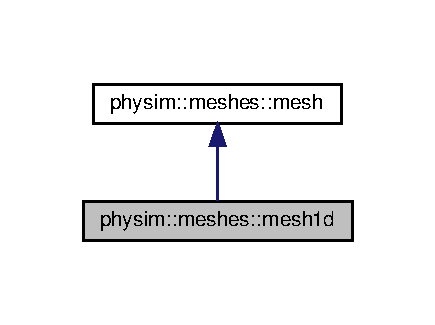
\includegraphics[width=209pt]{classphysim_1_1meshes_1_1mesh1d__inherit__graph}
\end{center}
\end{figure}


Collaboration diagram for physim\+:\+:meshes\+:\+:mesh1d\+:\nopagebreak
\begin{figure}[H]
\begin{center}
\leavevmode
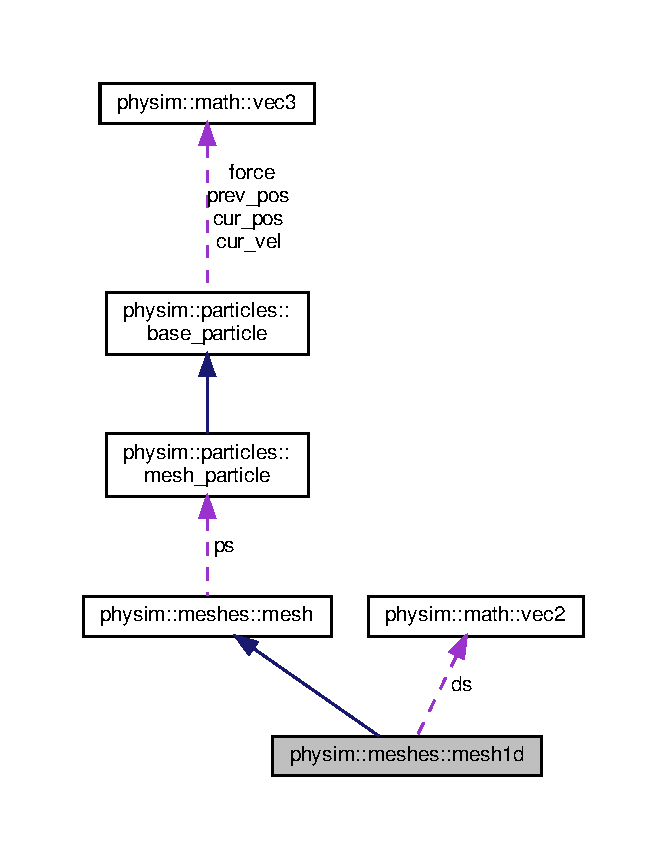
\includegraphics[width=320pt]{classphysim_1_1meshes_1_1mesh1d__coll__graph}
\end{center}
\end{figure}
\subsection*{Public Member Functions}
\begin{DoxyCompactItemize}
\item 
\mbox{\Hypertarget{classphysim_1_1meshes_1_1mesh1d_a6fe979fbcab7ff4534044d8d6fc9071e}\label{classphysim_1_1meshes_1_1mesh1d_a6fe979fbcab7ff4534044d8d6fc9071e}} 
\hyperlink{classphysim_1_1meshes_1_1mesh1d_a6fe979fbcab7ff4534044d8d6fc9071e}{mesh1d} ()
\begin{DoxyCompactList}\small\item\em Default constructor. \end{DoxyCompactList}\item 
\hyperlink{classphysim_1_1meshes_1_1mesh1d_a75cb535a4e9a65b8b1f269b02224b4cc}{mesh1d} (float ke, float kd)
\begin{DoxyCompactList}\small\item\em Constructor with parameters. \end{DoxyCompactList}\item 
\mbox{\Hypertarget{classphysim_1_1meshes_1_1mesh1d_a8b34a93773ce6e9bfb725510d77e58fc}\label{classphysim_1_1meshes_1_1mesh1d_a8b34a93773ce6e9bfb725510d77e58fc}} 
\hyperlink{classphysim_1_1meshes_1_1mesh1d_a8b34a93773ce6e9bfb725510d77e58fc}{$\sim$mesh1d} ()
\begin{DoxyCompactList}\small\item\em Destructor. \end{DoxyCompactList}\item 
void \hyperlink{classphysim_1_1meshes_1_1mesh1d_a6f2275fbab0ddfcbf523cc5a359e1d9c}{make\+\_\+initial\+\_\+state} ()
\begin{DoxyCompactList}\small\item\em Builds the initial state of the mesh. \end{DoxyCompactList}\item 
void \hyperlink{classphysim_1_1meshes_1_1mesh1d_abc53d477a2999654e09cabb0b5fd15ff}{update\+\_\+forces} ()
\begin{DoxyCompactList}\small\item\em Update the forces generated within the mesh. \end{DoxyCompactList}\item 
\mbox{\Hypertarget{classphysim_1_1meshes_1_1mesh1d_a1fe7bdb4b6775eccea56b40e4477c4a8}\label{classphysim_1_1meshes_1_1mesh1d_a1fe7bdb4b6775eccea56b40e4477c4a8}} 
void \hyperlink{classphysim_1_1meshes_1_1mesh1d_a1fe7bdb4b6775eccea56b40e4477c4a8}{clear} ()
\begin{DoxyCompactList}\small\item\em Frees the memory occupied by this mesh. \end{DoxyCompactList}\item 
void \hyperlink{classphysim_1_1meshes_1_1mesh1d_a7601dc6b7a0b59738bdf89c806fbd4ef}{simulate\+\_\+stretch} (bool s=true)
\begin{DoxyCompactList}\small\item\em Activates/\+Deactivates the simulation of stretch internal forces. \end{DoxyCompactList}\item 
void \hyperlink{classphysim_1_1meshes_1_1mesh1d_aaea453fcd1f5f41b6674da822bf53b2f}{simulate\+\_\+bend} (bool s=true)
\begin{DoxyCompactList}\small\item\em Activates/\+Deactivates the simulation of bending internal forces. \end{DoxyCompactList}\item 
bool \hyperlink{classphysim_1_1meshes_1_1mesh1d_acf2d9d0399ecbb4bdf3b521d94342258}{is\+\_\+simulating\+\_\+stretch} () const
\begin{DoxyCompactList}\small\item\em Returns whether stretch forces are actived. \end{DoxyCompactList}\item 
bool \hyperlink{classphysim_1_1meshes_1_1mesh1d_a9cd71d3d05385e30b5e7e330e5f5fb0e}{is\+\_\+simulating\+\_\+bend} () const
\begin{DoxyCompactList}\small\item\em Returns whether bend forces are actived. \end{DoxyCompactList}\end{DoxyCompactItemize}
\subsection*{Private Attributes}
\begin{DoxyCompactItemize}
\item 
\hyperlink{structphysim_1_1math_1_1vec2}{math\+::vec2} $\ast$ \hyperlink{classphysim_1_1meshes_1_1mesh1d_a9f185406b79496adfb33947591620ddf}{ds}
\begin{DoxyCompactList}\small\item\em Original distances between the particles. \end{DoxyCompactList}\item 
\mbox{\Hypertarget{classphysim_1_1meshes_1_1mesh1d_a2c5233fc91df5ae5ac41759e4d8419da}\label{classphysim_1_1meshes_1_1mesh1d_a2c5233fc91df5ae5ac41759e4d8419da}} 
bool \hyperlink{classphysim_1_1meshes_1_1mesh1d_a2c5233fc91df5ae5ac41759e4d8419da}{stretch}
\begin{DoxyCompactList}\small\item\em Simulate stretch forces. \end{DoxyCompactList}\item 
\mbox{\Hypertarget{classphysim_1_1meshes_1_1mesh1d_a941f796d30c2204e3aa995e984063355}\label{classphysim_1_1meshes_1_1mesh1d_a941f796d30c2204e3aa995e984063355}} 
bool \hyperlink{classphysim_1_1meshes_1_1mesh1d_a941f796d30c2204e3aa995e984063355}{shear}
\begin{DoxyCompactList}\small\item\em Simulate shear forces. \end{DoxyCompactList}\item 
\mbox{\Hypertarget{classphysim_1_1meshes_1_1mesh1d_a93d3f9fb656f309bf884333bafa9383e}\label{classphysim_1_1meshes_1_1mesh1d_a93d3f9fb656f309bf884333bafa9383e}} 
bool \hyperlink{classphysim_1_1meshes_1_1mesh1d_a93d3f9fb656f309bf884333bafa9383e}{bend}
\begin{DoxyCompactList}\small\item\em Simulate bend forces. \end{DoxyCompactList}\end{DoxyCompactItemize}
\subsection*{Additional Inherited Members}


\subsection{Detailed Description}
1-\/\+Dimensional spring mesh. 

This represents a set of \hyperlink{classphysim_1_1particles_1_1mesh__particle}{particles\+::mesh\+\_\+particle} where one particle is attached to at most two other particles.

If the local index of a particle is 0, then that particle is connected only to particle with index 1. Similarly, the particle with local index N -\/ 1 is only connected to that with index N -\/ 2. The other particles are connected to the particles with index $\pm 1$.

In this type of meshes, there two types of internal forces implemented by default\+:
\begin{DoxyItemize}
\item stretch\+: \hyperlink{classphysim_1_1meshes_1_1mesh1d_a2c5233fc91df5ae5ac41759e4d8419da}{stretch}.
\item bending\+: \hyperlink{classphysim_1_1meshes_1_1mesh1d_a93d3f9fb656f309bf884333bafa9383e}{bend}. These internal forces can be activated through the functions
\item \hyperlink{classphysim_1_1meshes_1_1mesh1d_a7601dc6b7a0b59738bdf89c806fbd4ef}{simulate\+\_\+stretch}.
\item \hyperlink{classphysim_1_1meshes_1_1mesh1d_aaea453fcd1f5f41b6674da822bf53b2f}{simulate\+\_\+bend}. with an appropriate value of their parameter. Depending on the type of mesh some of these forces may not be implemented. 
\end{DoxyItemize}

\subsection{Constructor \& Destructor Documentation}
\mbox{\Hypertarget{classphysim_1_1meshes_1_1mesh1d_a75cb535a4e9a65b8b1f269b02224b4cc}\label{classphysim_1_1meshes_1_1mesh1d_a75cb535a4e9a65b8b1f269b02224b4cc}} 
\index{physim\+::meshes\+::mesh1d@{physim\+::meshes\+::mesh1d}!mesh1d@{mesh1d}}
\index{mesh1d@{mesh1d}!physim\+::meshes\+::mesh1d@{physim\+::meshes\+::mesh1d}}
\subsubsection{\texorpdfstring{mesh1d()}{mesh1d()}}
{\footnotesize\ttfamily physim\+::meshes\+::mesh1d\+::mesh1d (\begin{DoxyParamCaption}\item[{float}]{ke,  }\item[{float}]{kd }\end{DoxyParamCaption})}



Constructor with parameters. 


\begin{DoxyParams}{Parameters}
{\em ke} & Elasticity parameter. \\
\hline
{\em kd} & Damping factor. \\
\hline
\end{DoxyParams}


\subsection{Member Function Documentation}
\mbox{\Hypertarget{classphysim_1_1meshes_1_1mesh1d_a9cd71d3d05385e30b5e7e330e5f5fb0e}\label{classphysim_1_1meshes_1_1mesh1d_a9cd71d3d05385e30b5e7e330e5f5fb0e}} 
\index{physim\+::meshes\+::mesh1d@{physim\+::meshes\+::mesh1d}!is\+\_\+simulating\+\_\+bend@{is\+\_\+simulating\+\_\+bend}}
\index{is\+\_\+simulating\+\_\+bend@{is\+\_\+simulating\+\_\+bend}!physim\+::meshes\+::mesh1d@{physim\+::meshes\+::mesh1d}}
\subsubsection{\texorpdfstring{is\+\_\+simulating\+\_\+bend()}{is\_simulating\_bend()}}
{\footnotesize\ttfamily bool physim\+::meshes\+::mesh1d\+::is\+\_\+simulating\+\_\+bend (\begin{DoxyParamCaption}{ }\end{DoxyParamCaption}) const}



Returns whether bend forces are actived. 

\begin{DoxyReturn}{Returns}
Returns the value of \hyperlink{classphysim_1_1meshes_1_1mesh1d_a93d3f9fb656f309bf884333bafa9383e}{bend}. 
\end{DoxyReturn}
\mbox{\Hypertarget{classphysim_1_1meshes_1_1mesh1d_acf2d9d0399ecbb4bdf3b521d94342258}\label{classphysim_1_1meshes_1_1mesh1d_acf2d9d0399ecbb4bdf3b521d94342258}} 
\index{physim\+::meshes\+::mesh1d@{physim\+::meshes\+::mesh1d}!is\+\_\+simulating\+\_\+stretch@{is\+\_\+simulating\+\_\+stretch}}
\index{is\+\_\+simulating\+\_\+stretch@{is\+\_\+simulating\+\_\+stretch}!physim\+::meshes\+::mesh1d@{physim\+::meshes\+::mesh1d}}
\subsubsection{\texorpdfstring{is\+\_\+simulating\+\_\+stretch()}{is\_simulating\_stretch()}}
{\footnotesize\ttfamily bool physim\+::meshes\+::mesh1d\+::is\+\_\+simulating\+\_\+stretch (\begin{DoxyParamCaption}{ }\end{DoxyParamCaption}) const}



Returns whether stretch forces are actived. 

\begin{DoxyReturn}{Returns}
Returns the value of \hyperlink{classphysim_1_1meshes_1_1mesh1d_a2c5233fc91df5ae5ac41759e4d8419da}{stretch}. 
\end{DoxyReturn}
\mbox{\Hypertarget{classphysim_1_1meshes_1_1mesh1d_a6f2275fbab0ddfcbf523cc5a359e1d9c}\label{classphysim_1_1meshes_1_1mesh1d_a6f2275fbab0ddfcbf523cc5a359e1d9c}} 
\index{physim\+::meshes\+::mesh1d@{physim\+::meshes\+::mesh1d}!make\+\_\+initial\+\_\+state@{make\+\_\+initial\+\_\+state}}
\index{make\+\_\+initial\+\_\+state@{make\+\_\+initial\+\_\+state}!physim\+::meshes\+::mesh1d@{physim\+::meshes\+::mesh1d}}
\subsubsection{\texorpdfstring{make\+\_\+initial\+\_\+state()}{make\_initial\_state()}}
{\footnotesize\ttfamily void physim\+::meshes\+::mesh1d\+::make\+\_\+initial\+\_\+state (\begin{DoxyParamCaption}{ }\end{DoxyParamCaption})\hspace{0.3cm}{\ttfamily [virtual]}}



Builds the initial state of the mesh. 

Records the initial distances between neighbouring particles.

\begin{DoxyPrecond}{Precondition}
All this mesh\textquotesingle{}s particles must have been initialised. 
\end{DoxyPrecond}


Implements \hyperlink{classphysim_1_1meshes_1_1mesh_a62f877dd42bc306ef70c76fc172f245f}{physim\+::meshes\+::mesh}.

\mbox{\Hypertarget{classphysim_1_1meshes_1_1mesh1d_aaea453fcd1f5f41b6674da822bf53b2f}\label{classphysim_1_1meshes_1_1mesh1d_aaea453fcd1f5f41b6674da822bf53b2f}} 
\index{physim\+::meshes\+::mesh1d@{physim\+::meshes\+::mesh1d}!simulate\+\_\+bend@{simulate\+\_\+bend}}
\index{simulate\+\_\+bend@{simulate\+\_\+bend}!physim\+::meshes\+::mesh1d@{physim\+::meshes\+::mesh1d}}
\subsubsection{\texorpdfstring{simulate\+\_\+bend()}{simulate\_bend()}}
{\footnotesize\ttfamily void physim\+::meshes\+::mesh1d\+::simulate\+\_\+bend (\begin{DoxyParamCaption}\item[{bool}]{s = {\ttfamily true} }\end{DoxyParamCaption})}



Activates/\+Deactivates the simulation of bending internal forces. 

Sets \hyperlink{classphysim_1_1meshes_1_1mesh1d_a93d3f9fb656f309bf884333bafa9383e}{bend} to the value of {\itshape s}. 
\begin{DoxyParams}{Parameters}
{\em s} & True or false depending on whether the simulation has to activated or deactivated. \\
\hline
\end{DoxyParams}
\mbox{\Hypertarget{classphysim_1_1meshes_1_1mesh1d_a7601dc6b7a0b59738bdf89c806fbd4ef}\label{classphysim_1_1meshes_1_1mesh1d_a7601dc6b7a0b59738bdf89c806fbd4ef}} 
\index{physim\+::meshes\+::mesh1d@{physim\+::meshes\+::mesh1d}!simulate\+\_\+stretch@{simulate\+\_\+stretch}}
\index{simulate\+\_\+stretch@{simulate\+\_\+stretch}!physim\+::meshes\+::mesh1d@{physim\+::meshes\+::mesh1d}}
\subsubsection{\texorpdfstring{simulate\+\_\+stretch()}{simulate\_stretch()}}
{\footnotesize\ttfamily void physim\+::meshes\+::mesh1d\+::simulate\+\_\+stretch (\begin{DoxyParamCaption}\item[{bool}]{s = {\ttfamily true} }\end{DoxyParamCaption})}



Activates/\+Deactivates the simulation of stretch internal forces. 

Sets \hyperlink{classphysim_1_1meshes_1_1mesh1d_a2c5233fc91df5ae5ac41759e4d8419da}{stretch} to the value of {\itshape s}. 
\begin{DoxyParams}{Parameters}
{\em s} & True or false depending on whether the simulation has to activated or deactivated. \\
\hline
\end{DoxyParams}
\mbox{\Hypertarget{classphysim_1_1meshes_1_1mesh1d_abc53d477a2999654e09cabb0b5fd15ff}\label{classphysim_1_1meshes_1_1mesh1d_abc53d477a2999654e09cabb0b5fd15ff}} 
\index{physim\+::meshes\+::mesh1d@{physim\+::meshes\+::mesh1d}!update\+\_\+forces@{update\+\_\+forces}}
\index{update\+\_\+forces@{update\+\_\+forces}!physim\+::meshes\+::mesh1d@{physim\+::meshes\+::mesh1d}}
\subsubsection{\texorpdfstring{update\+\_\+forces()}{update\_forces()}}
{\footnotesize\ttfamily void physim\+::meshes\+::mesh1d\+::update\+\_\+forces (\begin{DoxyParamCaption}{ }\end{DoxyParamCaption})\hspace{0.3cm}{\ttfamily [virtual]}}



Update the forces generated within the mesh. 

This method updates the forces acting on a particle {\itshape i} and its neighbouring particles. This includes stretch and beding forces.

\begin{DoxyPrecond}{Precondition}
The modification of the particle\textquotesingle{}s forces should not assume that particles start with null force (force equal to 0 in the three axes). Moreover, the initial state of the mesh must have been made (see \hyperlink{classphysim_1_1meshes_1_1mesh1d_a6f2275fbab0ddfcbf523cc5a359e1d9c}{make\+\_\+initial\+\_\+state}). 
\end{DoxyPrecond}


Implements \hyperlink{classphysim_1_1meshes_1_1mesh_ad7cad4cd454cce562c8c404ef09f8bd3}{physim\+::meshes\+::mesh}.



\subsection{Member Data Documentation}
\mbox{\Hypertarget{classphysim_1_1meshes_1_1mesh1d_a9f185406b79496adfb33947591620ddf}\label{classphysim_1_1meshes_1_1mesh1d_a9f185406b79496adfb33947591620ddf}} 
\index{physim\+::meshes\+::mesh1d@{physim\+::meshes\+::mesh1d}!ds@{ds}}
\index{ds@{ds}!physim\+::meshes\+::mesh1d@{physim\+::meshes\+::mesh1d}}
\subsubsection{\texorpdfstring{ds}{ds}}
{\footnotesize\ttfamily \hyperlink{structphysim_1_1math_1_1vec2}{math\+::vec2}$\ast$ physim\+::meshes\+::mesh1d\+::ds\hspace{0.3cm}{\ttfamily [private]}}



Original distances between the particles. 

Function \hyperlink{classphysim_1_1meshes_1_1mesh1d_a6f2275fbab0ddfcbf523cc5a359e1d9c}{make\+\_\+initial\+\_\+state} fills this vector with the distances between the particles\textquotesingle{} positions that they had prior to calling this method. The particles used for computing these distances are neighbouring particles.

The contents are formally defined as\+: stretch\+\_\+ds\mbox{[}i\mbox{]}.x = distance(particle i, particle i + 1) for i ranging in \mbox{[}0, N -\/ 2\mbox{]}.

stretch\+\_\+ds\mbox{[}i\mbox{]}.y = distance(particle i, particle i + 2) for i ranging in \mbox{[}0, N -\/ 3\mbox{]}.

The distances in the .x members are used for stretch forces.

The distances in the .y members are used for bend forces. 

The documentation for this class was generated from the following files\+:\begin{DoxyCompactItemize}
\item 
physim/meshes/mesh1d.\+hpp\item 
physim/meshes/mesh1d.\+cpp\end{DoxyCompactItemize}

\hypertarget{classphysim_1_1meshes_1_1mesh2d}{}\section{physim\+:\+:meshes\+:\+:mesh2d Class Reference}
\label{classphysim_1_1meshes_1_1mesh2d}\index{physim\+::meshes\+::mesh2d@{physim\+::meshes\+::mesh2d}}


2-\/\+Dimensional spring mesh.  




{\ttfamily \#include $<$mesh2d.\+hpp$>$}



Inheritance diagram for physim\+:\+:meshes\+:\+:mesh2d\+:\nopagebreak
\begin{figure}[H]
\begin{center}
\leavevmode
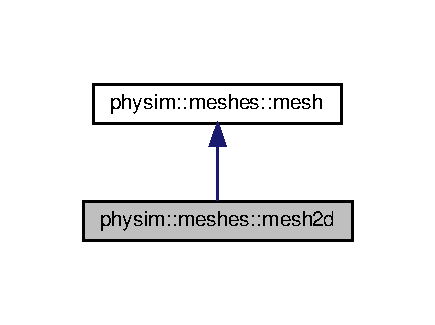
\includegraphics[width=209pt]{classphysim_1_1meshes_1_1mesh2d__inherit__graph}
\end{center}
\end{figure}


Collaboration diagram for physim\+:\+:meshes\+:\+:mesh2d\+:\nopagebreak
\begin{figure}[H]
\begin{center}
\leavevmode
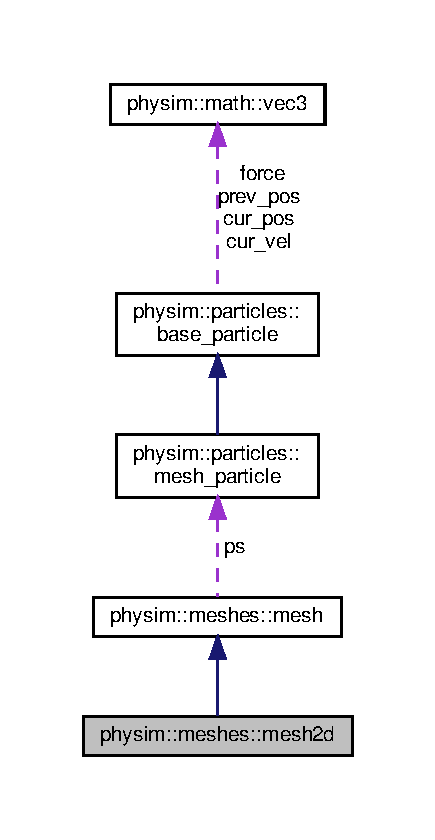
\includegraphics[width=209pt]{classphysim_1_1meshes_1_1mesh2d__coll__graph}
\end{center}
\end{figure}
\subsection*{Public Member Functions}
\begin{DoxyCompactItemize}
\item 
\mbox{\Hypertarget{classphysim_1_1meshes_1_1mesh2d_ae736ed194bb1c00bdd5fa1157ce0cc21}\label{classphysim_1_1meshes_1_1mesh2d_ae736ed194bb1c00bdd5fa1157ce0cc21}} 
\hyperlink{classphysim_1_1meshes_1_1mesh2d_ae736ed194bb1c00bdd5fa1157ce0cc21}{mesh2d} ()
\begin{DoxyCompactList}\small\item\em Default constructor. \end{DoxyCompactList}\item 
\hyperlink{classphysim_1_1meshes_1_1mesh2d_a4d5e184186bbe4e6e67cf6dd5d2bca5e}{mesh2d} (float ke, float kd)
\begin{DoxyCompactList}\small\item\em Constructor with parameters. \end{DoxyCompactList}\item 
\mbox{\Hypertarget{classphysim_1_1meshes_1_1mesh2d_a6b5ca67d5bd3796086d2d2893c1dbf4e}\label{classphysim_1_1meshes_1_1mesh2d_a6b5ca67d5bd3796086d2d2893c1dbf4e}} 
virtual \hyperlink{classphysim_1_1meshes_1_1mesh2d_a6b5ca67d5bd3796086d2d2893c1dbf4e}{$\sim$mesh2d} ()
\begin{DoxyCompactList}\small\item\em Destructor. \end{DoxyCompactList}\end{DoxyCompactItemize}
\subsection*{Additional Inherited Members}


\subsection{Detailed Description}
2-\/\+Dimensional spring mesh. 

A 2-\/dimensional mesh does not differ much from a 3-\/dimensional mesh. However, these are used mainly for cloth simulation. 

\subsection{Constructor \& Destructor Documentation}
\mbox{\Hypertarget{classphysim_1_1meshes_1_1mesh2d_a4d5e184186bbe4e6e67cf6dd5d2bca5e}\label{classphysim_1_1meshes_1_1mesh2d_a4d5e184186bbe4e6e67cf6dd5d2bca5e}} 
\index{physim\+::meshes\+::mesh2d@{physim\+::meshes\+::mesh2d}!mesh2d@{mesh2d}}
\index{mesh2d@{mesh2d}!physim\+::meshes\+::mesh2d@{physim\+::meshes\+::mesh2d}}
\subsubsection{\texorpdfstring{mesh2d()}{mesh2d()}}
{\footnotesize\ttfamily physim\+::meshes\+::mesh2d\+::mesh2d (\begin{DoxyParamCaption}\item[{float}]{ke,  }\item[{float}]{kd }\end{DoxyParamCaption})}



Constructor with parameters. 


\begin{DoxyParams}{Parameters}
{\em ke} & Elasticity parameter. \\
\hline
{\em kd} & Damping factor. \\
\hline
\end{DoxyParams}


The documentation for this class was generated from the following files\+:\begin{DoxyCompactItemize}
\item 
physim/meshes/mesh2d.\+hpp\item 
physim/meshes/mesh2d.\+cpp\end{DoxyCompactItemize}

\hypertarget{classphysim_1_1meshes_1_1mesh2d__regular}{}\section{physim\+:\+:meshes\+:\+:mesh2d\+\_\+regular Class Reference}
\label{classphysim_1_1meshes_1_1mesh2d__regular}\index{physim\+::meshes\+::mesh2d\+\_\+regular@{physim\+::meshes\+::mesh2d\+\_\+regular}}


2-\/\+Dimensional regular spring mesh.  




{\ttfamily \#include $<$mesh2d\+\_\+regular.\+hpp$>$}



Inheritance diagram for physim\+:\+:meshes\+:\+:mesh2d\+\_\+regular\+:\nopagebreak
\begin{figure}[H]
\begin{center}
\leavevmode
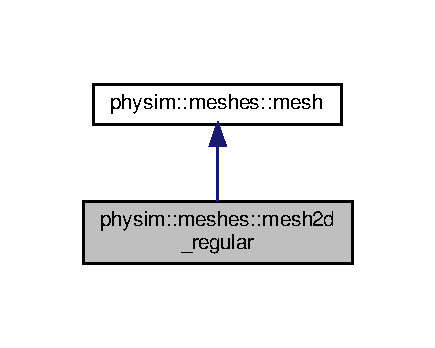
\includegraphics[width=209pt]{classphysim_1_1meshes_1_1mesh2d__regular__inherit__graph}
\end{center}
\end{figure}


Collaboration diagram for physim\+:\+:meshes\+:\+:mesh2d\+\_\+regular\+:\nopagebreak
\begin{figure}[H]
\begin{center}
\leavevmode
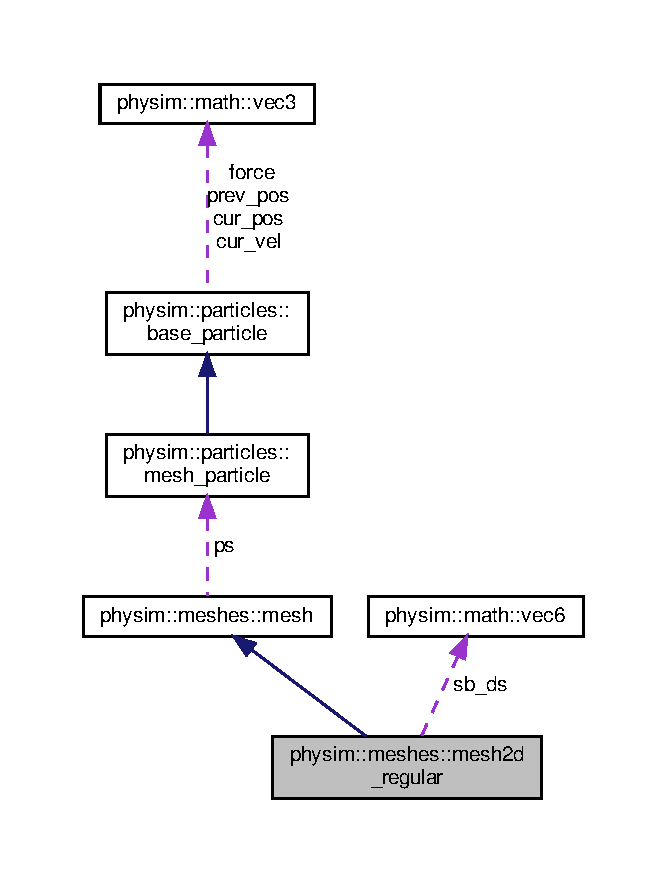
\includegraphics[width=320pt]{classphysim_1_1meshes_1_1mesh2d__regular__coll__graph}
\end{center}
\end{figure}
\subsection*{Public Member Functions}
\begin{DoxyCompactItemize}
\item 
\mbox{\Hypertarget{classphysim_1_1meshes_1_1mesh2d__regular_a2a8801b097cd6bccd6d6a088fa6f6d9f}\label{classphysim_1_1meshes_1_1mesh2d__regular_a2a8801b097cd6bccd6d6a088fa6f6d9f}} 
\hyperlink{classphysim_1_1meshes_1_1mesh2d__regular_a2a8801b097cd6bccd6d6a088fa6f6d9f}{mesh2d\+\_\+regular} ()
\begin{DoxyCompactList}\small\item\em Default constructor. \end{DoxyCompactList}\item 
\hyperlink{classphysim_1_1meshes_1_1mesh2d__regular_acaae970247d081125fc7c77368aafc07}{mesh2d\+\_\+regular} (float ke, float kd)
\begin{DoxyCompactList}\small\item\em Constructor with parameters. \end{DoxyCompactList}\item 
\mbox{\Hypertarget{classphysim_1_1meshes_1_1mesh2d__regular_aa33cccd404aa92abb6bf1c654054da9d}\label{classphysim_1_1meshes_1_1mesh2d__regular_aa33cccd404aa92abb6bf1c654054da9d}} 
virtual \hyperlink{classphysim_1_1meshes_1_1mesh2d__regular_aa33cccd404aa92abb6bf1c654054da9d}{$\sim$mesh2d\+\_\+regular} ()
\begin{DoxyCompactList}\small\item\em Destructor. \end{DoxyCompactList}\item 
void \hyperlink{classphysim_1_1meshes_1_1mesh2d__regular_ab05d404566850dd5a2d11814c3c25186}{make\+\_\+initial\+\_\+state} ()
\begin{DoxyCompactList}\small\item\em Builds the initial state of the mesh. \end{DoxyCompactList}\item 
void \hyperlink{classphysim_1_1meshes_1_1mesh2d__regular_aaf4e82b9231d79624224c3462cc18809}{update\+\_\+forces} ()
\begin{DoxyCompactList}\small\item\em Update the forces generated within the mesh. \end{DoxyCompactList}\item 
\mbox{\Hypertarget{classphysim_1_1meshes_1_1mesh2d__regular_a6881e0701bdbbaf06f0502edfa8baac8}\label{classphysim_1_1meshes_1_1mesh2d__regular_a6881e0701bdbbaf06f0502edfa8baac8}} 
void \hyperlink{classphysim_1_1meshes_1_1mesh2d__regular_a6881e0701bdbbaf06f0502edfa8baac8}{clear} ()
\begin{DoxyCompactList}\small\item\em Frees the memory occupied by this mesh. \end{DoxyCompactList}\item 
void \hyperlink{classphysim_1_1meshes_1_1mesh2d__regular_a6d9ccf2226fb57cc3ffc04fd9612acdd}{simulate\+\_\+stretch} (bool s=true)
\begin{DoxyCompactList}\small\item\em Activates/\+Deactivates the simulation of stretch internal forces. \end{DoxyCompactList}\item 
void \hyperlink{classphysim_1_1meshes_1_1mesh2d__regular_a36293f6559978144527fb829efd63ea2}{simulate\+\_\+shear} (bool s=true)
\begin{DoxyCompactList}\small\item\em Activates/\+Deactivates the simulation of shear internal forces. \end{DoxyCompactList}\item 
void \hyperlink{classphysim_1_1meshes_1_1mesh2d__regular_abc94712fdb508f126934bd2bde2cf867}{simulate\+\_\+bend} (bool s=true)
\begin{DoxyCompactList}\small\item\em Activates/\+Deactivates the simulation of bending internal forces. \end{DoxyCompactList}\item 
void \hyperlink{classphysim_1_1meshes_1_1mesh2d__regular_aa8d8eafaea92619a04b3bd1781c8aec7}{set\+\_\+dimensions} (size\+\_\+t r, size\+\_\+t c)
\begin{DoxyCompactList}\small\item\em Sets the number of rows and columns. \end{DoxyCompactList}\item 
bool \hyperlink{classphysim_1_1meshes_1_1mesh2d__regular_ad1674ad6c5d8d3ed7ec01767f63f2de5}{is\+\_\+simulating\+\_\+stretch} () const
\begin{DoxyCompactList}\small\item\em Returns whether stretch forces are actived. \end{DoxyCompactList}\item 
bool \hyperlink{classphysim_1_1meshes_1_1mesh2d__regular_a1620fec743604c7a9dd8b8c81344b615}{is\+\_\+simulating\+\_\+shear} () const
\begin{DoxyCompactList}\small\item\em Returns whether shear forces are actived. \end{DoxyCompactList}\item 
bool \hyperlink{classphysim_1_1meshes_1_1mesh2d__regular_a9410509a30c8416a11bc50d34820bafe}{is\+\_\+simulating\+\_\+bend} () const
\begin{DoxyCompactList}\small\item\em Returns whether bend forces are actived. \end{DoxyCompactList}\item 
void \hyperlink{classphysim_1_1meshes_1_1mesh2d__regular_a26fcf2ed9c0532a33e524a5f1728dbdf}{get\+\_\+dimensions} (size\+\_\+t \&r, size\+\_\+t \&c) const
\begin{DoxyCompactList}\small\item\em Gets the number of rows and columns. \end{DoxyCompactList}\item 
size\+\_\+t \hyperlink{classphysim_1_1meshes_1_1mesh2d__regular_a9ba9ff2e69bfcdb38a6362f35dbb1ba4}{get\+\_\+global\+\_\+index} (size\+\_\+t i, size\+\_\+t j) const
\begin{DoxyCompactList}\small\item\em Returns the index of a particle of the mesh. \end{DoxyCompactList}\end{DoxyCompactItemize}
\subsection*{Private Attributes}
\begin{DoxyCompactItemize}
\item 
\mbox{\Hypertarget{classphysim_1_1meshes_1_1mesh2d__regular_a5940b5ab5b5b67139d13c10e473b4894}\label{classphysim_1_1meshes_1_1mesh2d__regular_a5940b5ab5b5b67139d13c10e473b4894}} 
size\+\_\+t \hyperlink{classphysim_1_1meshes_1_1mesh2d__regular_a5940b5ab5b5b67139d13c10e473b4894}{R}
\begin{DoxyCompactList}\small\item\em Number of rows of the grid. \end{DoxyCompactList}\item 
\mbox{\Hypertarget{classphysim_1_1meshes_1_1mesh2d__regular_ae26a7e636588726103a835faf67b7771}\label{classphysim_1_1meshes_1_1mesh2d__regular_ae26a7e636588726103a835faf67b7771}} 
size\+\_\+t \hyperlink{classphysim_1_1meshes_1_1mesh2d__regular_ae26a7e636588726103a835faf67b7771}{C}
\begin{DoxyCompactList}\small\item\em Number of columns of the grid. \end{DoxyCompactList}\item 
\hyperlink{structphysim_1_1math_1_1vec6}{math\+::vec6} $\ast$ \hyperlink{classphysim_1_1meshes_1_1mesh2d__regular_ac3a70b7b6b37942d5174ddcc90703993}{sb\+\_\+ds}
\begin{DoxyCompactList}\small\item\em Original distances between the particles. \end{DoxyCompactList}\item 
\mbox{\Hypertarget{classphysim_1_1meshes_1_1mesh2d__regular_a3101edd8212afd9a35ad11c6666e26be}\label{classphysim_1_1meshes_1_1mesh2d__regular_a3101edd8212afd9a35ad11c6666e26be}} 
bool \hyperlink{classphysim_1_1meshes_1_1mesh2d__regular_a3101edd8212afd9a35ad11c6666e26be}{stretch}
\begin{DoxyCompactList}\small\item\em Simulate stretch forces. \end{DoxyCompactList}\item 
\mbox{\Hypertarget{classphysim_1_1meshes_1_1mesh2d__regular_af25bf35485aa0a40e21a10f4e472721a}\label{classphysim_1_1meshes_1_1mesh2d__regular_af25bf35485aa0a40e21a10f4e472721a}} 
bool \hyperlink{classphysim_1_1meshes_1_1mesh2d__regular_af25bf35485aa0a40e21a10f4e472721a}{shear}
\begin{DoxyCompactList}\small\item\em Simulate shear forces. \end{DoxyCompactList}\item 
\mbox{\Hypertarget{classphysim_1_1meshes_1_1mesh2d__regular_ab031a8ece45555e421c031b7c3fff4bd}\label{classphysim_1_1meshes_1_1mesh2d__regular_ab031a8ece45555e421c031b7c3fff4bd}} 
bool \hyperlink{classphysim_1_1meshes_1_1mesh2d__regular_ab031a8ece45555e421c031b7c3fff4bd}{bend}
\begin{DoxyCompactList}\small\item\em Simulate bend forces. \end{DoxyCompactList}\end{DoxyCompactItemize}
\subsection*{Additional Inherited Members}


\subsection{Detailed Description}
2-\/\+Dimensional regular spring mesh. 

This mesh\textquotesingle{}s springs are organised in a grid\+: the particles at the four corners have two neighbours, the particles at the border of the grid (without considering the corners) have three neighbours, and the rest have four.

By neighbours it should be understood the immediate particle in the grid. That is, in a grid of {\itshape R} and {\itshape C} particles in each dimension the particle at $(i,j)\:|\: 0 \le i \le R - 1, 0 \le j \le C - 1$ has as neighbours the particles at $(i-1,j),(i+1,j),(i,j-1),(i,j+1)$.

In this type of meshes, there three types of internal forces implemented by default\+:
\begin{DoxyItemize}
\item stretch\+: \hyperlink{classphysim_1_1meshes_1_1mesh2d__regular_a3101edd8212afd9a35ad11c6666e26be}{stretch}.
\item shear\+: \hyperlink{classphysim_1_1meshes_1_1mesh2d__regular_af25bf35485aa0a40e21a10f4e472721a}{shear}.
\item bending\+: \hyperlink{classphysim_1_1meshes_1_1mesh2d__regular_ab031a8ece45555e421c031b7c3fff4bd}{bend}. These internal forces can be activated through the functions
\item \hyperlink{classphysim_1_1meshes_1_1mesh2d__regular_a6d9ccf2226fb57cc3ffc04fd9612acdd}{simulate\+\_\+stretch}.
\item \hyperlink{classphysim_1_1meshes_1_1mesh2d__regular_a36293f6559978144527fb829efd63ea2}{simulate\+\_\+shear}.
\item \hyperlink{classphysim_1_1meshes_1_1mesh2d__regular_abc94712fdb508f126934bd2bde2cf867}{simulate\+\_\+bend}. with an appropriate value of their parameter. Depending on the type of mesh some of these forces may not be implemented. 
\end{DoxyItemize}

\subsection{Constructor \& Destructor Documentation}
\mbox{\Hypertarget{classphysim_1_1meshes_1_1mesh2d__regular_acaae970247d081125fc7c77368aafc07}\label{classphysim_1_1meshes_1_1mesh2d__regular_acaae970247d081125fc7c77368aafc07}} 
\index{physim\+::meshes\+::mesh2d\+\_\+regular@{physim\+::meshes\+::mesh2d\+\_\+regular}!mesh2d\+\_\+regular@{mesh2d\+\_\+regular}}
\index{mesh2d\+\_\+regular@{mesh2d\+\_\+regular}!physim\+::meshes\+::mesh2d\+\_\+regular@{physim\+::meshes\+::mesh2d\+\_\+regular}}
\subsubsection{\texorpdfstring{mesh2d\+\_\+regular()}{mesh2d\_regular()}}
{\footnotesize\ttfamily physim\+::meshes\+::mesh2d\+\_\+regular\+::mesh2d\+\_\+regular (\begin{DoxyParamCaption}\item[{float}]{ke,  }\item[{float}]{kd }\end{DoxyParamCaption})}



Constructor with parameters. 


\begin{DoxyParams}{Parameters}
{\em ke} & Elasticity parameter. \\
\hline
{\em kd} & Damping factor. \\
\hline
\end{DoxyParams}


\subsection{Member Function Documentation}
\mbox{\Hypertarget{classphysim_1_1meshes_1_1mesh2d__regular_a26fcf2ed9c0532a33e524a5f1728dbdf}\label{classphysim_1_1meshes_1_1mesh2d__regular_a26fcf2ed9c0532a33e524a5f1728dbdf}} 
\index{physim\+::meshes\+::mesh2d\+\_\+regular@{physim\+::meshes\+::mesh2d\+\_\+regular}!get\+\_\+dimensions@{get\+\_\+dimensions}}
\index{get\+\_\+dimensions@{get\+\_\+dimensions}!physim\+::meshes\+::mesh2d\+\_\+regular@{physim\+::meshes\+::mesh2d\+\_\+regular}}
\subsubsection{\texorpdfstring{get\+\_\+dimensions()}{get\_dimensions()}}
{\footnotesize\ttfamily void physim\+::meshes\+::mesh2d\+\_\+regular\+::get\+\_\+dimensions (\begin{DoxyParamCaption}\item[{size\+\_\+t \&}]{r,  }\item[{size\+\_\+t \&}]{c }\end{DoxyParamCaption}) const}



Gets the number of rows and columns. 


\begin{DoxyParams}[1]{Parameters}
\mbox{\tt out}  & {\em r} & Number of rows. \\
\hline
\mbox{\tt out}  & {\em c} & Number of columns. \\
\hline
\end{DoxyParams}
\mbox{\Hypertarget{classphysim_1_1meshes_1_1mesh2d__regular_a9ba9ff2e69bfcdb38a6362f35dbb1ba4}\label{classphysim_1_1meshes_1_1mesh2d__regular_a9ba9ff2e69bfcdb38a6362f35dbb1ba4}} 
\index{physim\+::meshes\+::mesh2d\+\_\+regular@{physim\+::meshes\+::mesh2d\+\_\+regular}!get\+\_\+global\+\_\+index@{get\+\_\+global\+\_\+index}}
\index{get\+\_\+global\+\_\+index@{get\+\_\+global\+\_\+index}!physim\+::meshes\+::mesh2d\+\_\+regular@{physim\+::meshes\+::mesh2d\+\_\+regular}}
\subsubsection{\texorpdfstring{get\+\_\+global\+\_\+index()}{get\_global\_index()}}
{\footnotesize\ttfamily size\+\_\+t physim\+::meshes\+::mesh2d\+\_\+regular\+::get\+\_\+global\+\_\+index (\begin{DoxyParamCaption}\item[{size\+\_\+t}]{i,  }\item[{size\+\_\+t}]{j }\end{DoxyParamCaption}) const}



Returns the index of a particle of the mesh. 


\begin{DoxyParams}{Parameters}
{\em i} & Row index. \\
\hline
{\em j} & Column index. \\
\hline
\end{DoxyParams}
\begin{DoxyReturn}{Returns}
Returns the index of the particle at row {\itshape i} and column {\itshape j} as a single integer. 
\end{DoxyReturn}
\mbox{\Hypertarget{classphysim_1_1meshes_1_1mesh2d__regular_a9410509a30c8416a11bc50d34820bafe}\label{classphysim_1_1meshes_1_1mesh2d__regular_a9410509a30c8416a11bc50d34820bafe}} 
\index{physim\+::meshes\+::mesh2d\+\_\+regular@{physim\+::meshes\+::mesh2d\+\_\+regular}!is\+\_\+simulating\+\_\+bend@{is\+\_\+simulating\+\_\+bend}}
\index{is\+\_\+simulating\+\_\+bend@{is\+\_\+simulating\+\_\+bend}!physim\+::meshes\+::mesh2d\+\_\+regular@{physim\+::meshes\+::mesh2d\+\_\+regular}}
\subsubsection{\texorpdfstring{is\+\_\+simulating\+\_\+bend()}{is\_simulating\_bend()}}
{\footnotesize\ttfamily bool physim\+::meshes\+::mesh2d\+\_\+regular\+::is\+\_\+simulating\+\_\+bend (\begin{DoxyParamCaption}{ }\end{DoxyParamCaption}) const}



Returns whether bend forces are actived. 

\begin{DoxyReturn}{Returns}
Returns the value of \hyperlink{classphysim_1_1meshes_1_1mesh2d__regular_ab031a8ece45555e421c031b7c3fff4bd}{bend}. 
\end{DoxyReturn}
\mbox{\Hypertarget{classphysim_1_1meshes_1_1mesh2d__regular_a1620fec743604c7a9dd8b8c81344b615}\label{classphysim_1_1meshes_1_1mesh2d__regular_a1620fec743604c7a9dd8b8c81344b615}} 
\index{physim\+::meshes\+::mesh2d\+\_\+regular@{physim\+::meshes\+::mesh2d\+\_\+regular}!is\+\_\+simulating\+\_\+shear@{is\+\_\+simulating\+\_\+shear}}
\index{is\+\_\+simulating\+\_\+shear@{is\+\_\+simulating\+\_\+shear}!physim\+::meshes\+::mesh2d\+\_\+regular@{physim\+::meshes\+::mesh2d\+\_\+regular}}
\subsubsection{\texorpdfstring{is\+\_\+simulating\+\_\+shear()}{is\_simulating\_shear()}}
{\footnotesize\ttfamily bool physim\+::meshes\+::mesh2d\+\_\+regular\+::is\+\_\+simulating\+\_\+shear (\begin{DoxyParamCaption}{ }\end{DoxyParamCaption}) const}



Returns whether shear forces are actived. 

\begin{DoxyReturn}{Returns}
Returns the value of \hyperlink{classphysim_1_1meshes_1_1mesh2d__regular_af25bf35485aa0a40e21a10f4e472721a}{shear}. 
\end{DoxyReturn}
\mbox{\Hypertarget{classphysim_1_1meshes_1_1mesh2d__regular_ad1674ad6c5d8d3ed7ec01767f63f2de5}\label{classphysim_1_1meshes_1_1mesh2d__regular_ad1674ad6c5d8d3ed7ec01767f63f2de5}} 
\index{physim\+::meshes\+::mesh2d\+\_\+regular@{physim\+::meshes\+::mesh2d\+\_\+regular}!is\+\_\+simulating\+\_\+stretch@{is\+\_\+simulating\+\_\+stretch}}
\index{is\+\_\+simulating\+\_\+stretch@{is\+\_\+simulating\+\_\+stretch}!physim\+::meshes\+::mesh2d\+\_\+regular@{physim\+::meshes\+::mesh2d\+\_\+regular}}
\subsubsection{\texorpdfstring{is\+\_\+simulating\+\_\+stretch()}{is\_simulating\_stretch()}}
{\footnotesize\ttfamily bool physim\+::meshes\+::mesh2d\+\_\+regular\+::is\+\_\+simulating\+\_\+stretch (\begin{DoxyParamCaption}{ }\end{DoxyParamCaption}) const}



Returns whether stretch forces are actived. 

\begin{DoxyReturn}{Returns}
Returns the value of \hyperlink{classphysim_1_1meshes_1_1mesh2d__regular_a3101edd8212afd9a35ad11c6666e26be}{stretch}. 
\end{DoxyReturn}
\mbox{\Hypertarget{classphysim_1_1meshes_1_1mesh2d__regular_ab05d404566850dd5a2d11814c3c25186}\label{classphysim_1_1meshes_1_1mesh2d__regular_ab05d404566850dd5a2d11814c3c25186}} 
\index{physim\+::meshes\+::mesh2d\+\_\+regular@{physim\+::meshes\+::mesh2d\+\_\+regular}!make\+\_\+initial\+\_\+state@{make\+\_\+initial\+\_\+state}}
\index{make\+\_\+initial\+\_\+state@{make\+\_\+initial\+\_\+state}!physim\+::meshes\+::mesh2d\+\_\+regular@{physim\+::meshes\+::mesh2d\+\_\+regular}}
\subsubsection{\texorpdfstring{make\+\_\+initial\+\_\+state()}{make\_initial\_state()}}
{\footnotesize\ttfamily void physim\+::meshes\+::mesh2d\+\_\+regular\+::make\+\_\+initial\+\_\+state (\begin{DoxyParamCaption}{ }\end{DoxyParamCaption})\hspace{0.3cm}{\ttfamily [virtual]}}



Builds the initial state of the mesh. 

Records the initial distances between neighbouring particles.

\begin{DoxyPrecond}{Precondition}
All this mesh\textquotesingle{}s particles must have been initialised. 
\end{DoxyPrecond}


Implements \hyperlink{classphysim_1_1meshes_1_1mesh_a62f877dd42bc306ef70c76fc172f245f}{physim\+::meshes\+::mesh}.

\mbox{\Hypertarget{classphysim_1_1meshes_1_1mesh2d__regular_aa8d8eafaea92619a04b3bd1781c8aec7}\label{classphysim_1_1meshes_1_1mesh2d__regular_aa8d8eafaea92619a04b3bd1781c8aec7}} 
\index{physim\+::meshes\+::mesh2d\+\_\+regular@{physim\+::meshes\+::mesh2d\+\_\+regular}!set\+\_\+dimensions@{set\+\_\+dimensions}}
\index{set\+\_\+dimensions@{set\+\_\+dimensions}!physim\+::meshes\+::mesh2d\+\_\+regular@{physim\+::meshes\+::mesh2d\+\_\+regular}}
\subsubsection{\texorpdfstring{set\+\_\+dimensions()}{set\_dimensions()}}
{\footnotesize\ttfamily void physim\+::meshes\+::mesh2d\+\_\+regular\+::set\+\_\+dimensions (\begin{DoxyParamCaption}\item[{size\+\_\+t}]{r,  }\item[{size\+\_\+t}]{c }\end{DoxyParamCaption})}



Sets the number of rows and columns. 


\begin{DoxyParams}{Parameters}
{\em r} & Number of rows, at least 2. \\
\hline
{\em c} & Number of columns, at least 2. \\
\hline
\end{DoxyParams}
\begin{DoxyPrecond}{Precondition}
The particles of this mesh must have been allocated. The dimensions used must be equal to \hyperlink{classphysim_1_1meshes_1_1mesh_a5642217313d7dae9f873f01fad682ff2}{N} \+: r$\ast$c = N. 
\end{DoxyPrecond}
\mbox{\Hypertarget{classphysim_1_1meshes_1_1mesh2d__regular_abc94712fdb508f126934bd2bde2cf867}\label{classphysim_1_1meshes_1_1mesh2d__regular_abc94712fdb508f126934bd2bde2cf867}} 
\index{physim\+::meshes\+::mesh2d\+\_\+regular@{physim\+::meshes\+::mesh2d\+\_\+regular}!simulate\+\_\+bend@{simulate\+\_\+bend}}
\index{simulate\+\_\+bend@{simulate\+\_\+bend}!physim\+::meshes\+::mesh2d\+\_\+regular@{physim\+::meshes\+::mesh2d\+\_\+regular}}
\subsubsection{\texorpdfstring{simulate\+\_\+bend()}{simulate\_bend()}}
{\footnotesize\ttfamily void physim\+::meshes\+::mesh2d\+\_\+regular\+::simulate\+\_\+bend (\begin{DoxyParamCaption}\item[{bool}]{s = {\ttfamily true} }\end{DoxyParamCaption})}



Activates/\+Deactivates the simulation of bending internal forces. 

Sets \hyperlink{classphysim_1_1meshes_1_1mesh2d__regular_ab031a8ece45555e421c031b7c3fff4bd}{bend} to the value of {\itshape s}. 
\begin{DoxyParams}{Parameters}
{\em s} & True or false depending on whether the simulation has to activated or deactivated. \\
\hline
\end{DoxyParams}
\mbox{\Hypertarget{classphysim_1_1meshes_1_1mesh2d__regular_a36293f6559978144527fb829efd63ea2}\label{classphysim_1_1meshes_1_1mesh2d__regular_a36293f6559978144527fb829efd63ea2}} 
\index{physim\+::meshes\+::mesh2d\+\_\+regular@{physim\+::meshes\+::mesh2d\+\_\+regular}!simulate\+\_\+shear@{simulate\+\_\+shear}}
\index{simulate\+\_\+shear@{simulate\+\_\+shear}!physim\+::meshes\+::mesh2d\+\_\+regular@{physim\+::meshes\+::mesh2d\+\_\+regular}}
\subsubsection{\texorpdfstring{simulate\+\_\+shear()}{simulate\_shear()}}
{\footnotesize\ttfamily void physim\+::meshes\+::mesh2d\+\_\+regular\+::simulate\+\_\+shear (\begin{DoxyParamCaption}\item[{bool}]{s = {\ttfamily true} }\end{DoxyParamCaption})}



Activates/\+Deactivates the simulation of shear internal forces. 

Sets \hyperlink{classphysim_1_1meshes_1_1mesh2d__regular_af25bf35485aa0a40e21a10f4e472721a}{shear} to the value of {\itshape s}. 
\begin{DoxyParams}{Parameters}
{\em s} & True or false depending on whether the simulation has to activated or deactivated. \\
\hline
\end{DoxyParams}
\mbox{\Hypertarget{classphysim_1_1meshes_1_1mesh2d__regular_a6d9ccf2226fb57cc3ffc04fd9612acdd}\label{classphysim_1_1meshes_1_1mesh2d__regular_a6d9ccf2226fb57cc3ffc04fd9612acdd}} 
\index{physim\+::meshes\+::mesh2d\+\_\+regular@{physim\+::meshes\+::mesh2d\+\_\+regular}!simulate\+\_\+stretch@{simulate\+\_\+stretch}}
\index{simulate\+\_\+stretch@{simulate\+\_\+stretch}!physim\+::meshes\+::mesh2d\+\_\+regular@{physim\+::meshes\+::mesh2d\+\_\+regular}}
\subsubsection{\texorpdfstring{simulate\+\_\+stretch()}{simulate\_stretch()}}
{\footnotesize\ttfamily void physim\+::meshes\+::mesh2d\+\_\+regular\+::simulate\+\_\+stretch (\begin{DoxyParamCaption}\item[{bool}]{s = {\ttfamily true} }\end{DoxyParamCaption})}



Activates/\+Deactivates the simulation of stretch internal forces. 

Sets \hyperlink{classphysim_1_1meshes_1_1mesh2d__regular_a3101edd8212afd9a35ad11c6666e26be}{stretch} to the value of {\itshape s}. 
\begin{DoxyParams}{Parameters}
{\em s} & True or false depending on whether the simulation has to activated or deactivated. \\
\hline
\end{DoxyParams}
\mbox{\Hypertarget{classphysim_1_1meshes_1_1mesh2d__regular_aaf4e82b9231d79624224c3462cc18809}\label{classphysim_1_1meshes_1_1mesh2d__regular_aaf4e82b9231d79624224c3462cc18809}} 
\index{physim\+::meshes\+::mesh2d\+\_\+regular@{physim\+::meshes\+::mesh2d\+\_\+regular}!update\+\_\+forces@{update\+\_\+forces}}
\index{update\+\_\+forces@{update\+\_\+forces}!physim\+::meshes\+::mesh2d\+\_\+regular@{physim\+::meshes\+::mesh2d\+\_\+regular}}
\subsubsection{\texorpdfstring{update\+\_\+forces()}{update\_forces()}}
{\footnotesize\ttfamily void physim\+::meshes\+::mesh2d\+\_\+regular\+::update\+\_\+forces (\begin{DoxyParamCaption}{ }\end{DoxyParamCaption})\hspace{0.3cm}{\ttfamily [virtual]}}



Update the forces generated within the mesh. 

This method updates the forces acting on a particle {\itshape i} and its neighbouring particles. This includes stretch and beding forces.

\begin{DoxyPrecond}{Precondition}
The modification of the particle\textquotesingle{}s forces should not assume that particles start with null force (force equal to 0 in the three axes). Moreover, the initial state of the mesh must have been made (see \hyperlink{classphysim_1_1meshes_1_1mesh2d__regular_ab05d404566850dd5a2d11814c3c25186}{make\+\_\+initial\+\_\+state}). 
\end{DoxyPrecond}


Implements \hyperlink{classphysim_1_1meshes_1_1mesh_ad7cad4cd454cce562c8c404ef09f8bd3}{physim\+::meshes\+::mesh}.



\subsection{Member Data Documentation}
\mbox{\Hypertarget{classphysim_1_1meshes_1_1mesh2d__regular_ac3a70b7b6b37942d5174ddcc90703993}\label{classphysim_1_1meshes_1_1mesh2d__regular_ac3a70b7b6b37942d5174ddcc90703993}} 
\index{physim\+::meshes\+::mesh2d\+\_\+regular@{physim\+::meshes\+::mesh2d\+\_\+regular}!sb\+\_\+ds@{sb\+\_\+ds}}
\index{sb\+\_\+ds@{sb\+\_\+ds}!physim\+::meshes\+::mesh2d\+\_\+regular@{physim\+::meshes\+::mesh2d\+\_\+regular}}
\subsubsection{\texorpdfstring{sb\+\_\+ds}{sb\_ds}}
{\footnotesize\ttfamily \hyperlink{structphysim_1_1math_1_1vec6}{math\+::vec6}$\ast$ physim\+::meshes\+::mesh2d\+\_\+regular\+::sb\+\_\+ds\hspace{0.3cm}{\ttfamily [private]}}



Original distances between the particles. 

Function \hyperlink{classphysim_1_1meshes_1_1mesh2d__regular_ab05d404566850dd5a2d11814c3c25186}{make\+\_\+initial\+\_\+state} fills this vector with the distances between the particles that they had prior to calling this method.

For a particle ({\itshape i}, {\itshape j}) the original distances are\+:
\begin{DoxyItemize}
\item Stretch
\begin{DoxyItemize}
\item distance to (i, j + 1)\+: in member {\itshape x}.
\item distance to (i + 1, j)\+: in member {\itshape y}. for $0 \le i \le R - 2, 0 \le j \le C - 2$.
\end{DoxyItemize}
\item Bend
\begin{DoxyItemize}
\item distance to (i, j + 2)\+: in member {\itshape z}.
\item distance to (i + 2, j)\+: in member {\itshape u}. for $0 \le i \le R - 3, 0 \le j \le C - 3$.
\end{DoxyItemize}
\item Shear
\begin{DoxyItemize}
\item distance to (i -\/ 1, j + 1)\+: in member {\itshape v}. for $1 \le i \le R - 1, 0 \le j \le C - 2$.
\item distance to (i + 1, j + 1)\+: in member {\itshape w}. for $0 \le i \le R - 2, 0 \le j \le C - 2$.
\end{DoxyItemize}
\end{DoxyItemize}

where {\itshape C} is the number of columns (see \hyperlink{classphysim_1_1meshes_1_1mesh2d__regular_ae26a7e636588726103a835faf67b7771}{C}), and {\itshape R} is the number of rows (see \hyperlink{classphysim_1_1meshes_1_1mesh2d__regular_a5940b5ab5b5b67139d13c10e473b4894}{R}).

As a side note, there are some members that are not used at all. These are\+:
\begin{DoxyItemize}
\item members {\itshape z},{\itshape u}, for particles $(R-2,j), (i,C-2)$, for $0 \le i \le R - 2$ and $0 \le j \le C - 2$.
\item members {\itshape v}, for particles $(0,j)$, for $0 \le j \le C - 2$.
\item members {\itshape w}, for particles $(R-1,j)$, for $0 \le j \le C - 2$.
\end{DoxyItemize}

where {\itshape C} is the number of columns (see \hyperlink{classphysim_1_1meshes_1_1mesh2d__regular_ae26a7e636588726103a835faf67b7771}{C}), and {\itshape R} is the number of rows (see \hyperlink{classphysim_1_1meshes_1_1mesh2d__regular_a5940b5ab5b5b67139d13c10e473b4894}{R}). 

The documentation for this class was generated from the following files\+:\begin{DoxyCompactItemize}
\item 
physim/meshes/mesh2d\+\_\+regular.\+hpp\item 
physim/meshes/mesh2d\+\_\+regular.\+cpp\end{DoxyCompactItemize}

\hypertarget{classphysim_1_1particles_1_1mesh__particle}{}\section{physim\+:\+:particles\+:\+:mesh\+\_\+particle Class Reference}
\label{classphysim_1_1particles_1_1mesh__particle}\index{physim\+::particles\+::mesh\+\_\+particle@{physim\+::particles\+::mesh\+\_\+particle}}


Class implementing a mesh particle.  




{\ttfamily \#include $<$mesh\+\_\+particle.\+hpp$>$}



Inheritance diagram for physim\+:\+:particles\+:\+:mesh\+\_\+particle\+:\nopagebreak
\begin{figure}[H]
\begin{center}
\leavevmode
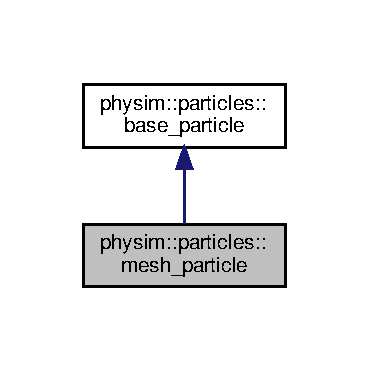
\includegraphics[width=177pt]{classphysim_1_1particles_1_1mesh__particle__inherit__graph}
\end{center}
\end{figure}


Collaboration diagram for physim\+:\+:particles\+:\+:mesh\+\_\+particle\+:\nopagebreak
\begin{figure}[H]
\begin{center}
\leavevmode
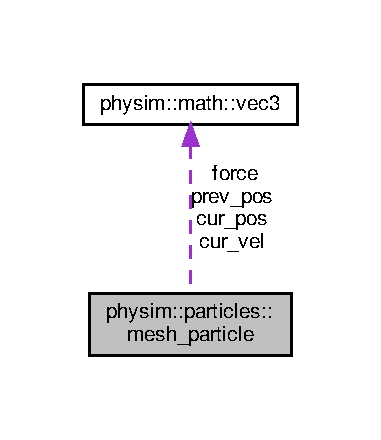
\includegraphics[width=183pt]{classphysim_1_1particles_1_1mesh__particle__coll__graph}
\end{center}
\end{figure}
\subsection*{Public Member Functions}
\begin{DoxyCompactItemize}
\item 
\mbox{\Hypertarget{classphysim_1_1particles_1_1mesh__particle_a0d7ccc38aee9b4cdeb5f66712d281040}\label{classphysim_1_1particles_1_1mesh__particle_a0d7ccc38aee9b4cdeb5f66712d281040}} 
\hyperlink{classphysim_1_1particles_1_1mesh__particle_a0d7ccc38aee9b4cdeb5f66712d281040}{mesh\+\_\+particle} ()
\begin{DoxyCompactList}\small\item\em Default constructor. \end{DoxyCompactList}\item 
\mbox{\Hypertarget{classphysim_1_1particles_1_1mesh__particle_a157eed705543d26a39ca4de632845699}\label{classphysim_1_1particles_1_1mesh__particle_a157eed705543d26a39ca4de632845699}} 
\hyperlink{classphysim_1_1particles_1_1mesh__particle_a157eed705543d26a39ca4de632845699}{mesh\+\_\+particle} (const \hyperlink{classphysim_1_1particles_1_1mesh__particle}{mesh\+\_\+particle} \&p)
\begin{DoxyCompactList}\small\item\em Copy constructor. \end{DoxyCompactList}\item 
\mbox{\Hypertarget{classphysim_1_1particles_1_1mesh__particle_acb853a925c65cd562252392ec754d614}\label{classphysim_1_1particles_1_1mesh__particle_acb853a925c65cd562252392ec754d614}} 
virtual \hyperlink{classphysim_1_1particles_1_1mesh__particle_acb853a925c65cd562252392ec754d614}{$\sim$mesh\+\_\+particle} ()
\begin{DoxyCompactList}\small\item\em Destructor. \end{DoxyCompactList}\item 
virtual void \hyperlink{classphysim_1_1particles_1_1mesh__particle_a1b3c3eac1e62296c2facd8c9d9b84608}{init} ()
\begin{DoxyCompactList}\small\item\em Initialises all particle\textquotesingle{}s attributes, most of them to null values. \end{DoxyCompactList}\item 
\mbox{\Hypertarget{classphysim_1_1particles_1_1mesh__particle_afb35d487caf79656b4e433ad34b0d8ac}\label{classphysim_1_1particles_1_1mesh__particle_afb35d487caf79656b4e433ad34b0d8ac}} 
virtual \hyperlink{namespacephysim_1_1particles_a068e6cda6626fbd381c07a9835425b08}{particle\+\_\+type} \hyperlink{classphysim_1_1particles_1_1mesh__particle_afb35d487caf79656b4e433ad34b0d8ac}{get\+\_\+particle\+\_\+type} () const
\begin{DoxyCompactList}\small\item\em Returns the type of this particle. \end{DoxyCompactList}\end{DoxyCompactItemize}
\subsection*{Public Attributes}
\begin{DoxyCompactItemize}
\item 
\mbox{\Hypertarget{classphysim_1_1particles_1_1mesh__particle_adf14d64e9effa2bcf5cb84a537bd8027}\label{classphysim_1_1particles_1_1mesh__particle_adf14d64e9effa2bcf5cb84a537bd8027}} 
float \hyperlink{classphysim_1_1particles_1_1mesh__particle_adf14d64e9effa2bcf5cb84a537bd8027}{charge}
\begin{DoxyCompactList}\small\item\em Electrical charge of the particle \mbox{[}C\mbox{]}. \end{DoxyCompactList}\item 
bool \hyperlink{classphysim_1_1particles_1_1mesh__particle_a5813a57507d8a3539a1534dfd1b74883}{fixed}
\begin{DoxyCompactList}\small\item\em Is this particle fixed? \end{DoxyCompactList}\end{DoxyCompactItemize}
\subsection*{Private Member Functions}
\begin{DoxyCompactItemize}
\item 
void \hyperlink{classphysim_1_1particles_1_1mesh__particle_acf394e0f807a6105e579750afbadeaea}{partial\+\_\+init} ()
\begin{DoxyCompactList}\small\item\em Initialises this class\textquotesingle{}s attributes. \end{DoxyCompactList}\end{DoxyCompactItemize}


\subsection{Detailed Description}
Class implementing a mesh particle. 

A particle is a 0-\/dimensional object, subject to several forces. It can also collide with other objects in the scene (geometrical objects, see namespace \hyperlink{namespacephysim_1_1geometric}{physim\+::geometric}) but not with other particles. 

\subsection{Member Function Documentation}
\mbox{\Hypertarget{classphysim_1_1particles_1_1mesh__particle_a1b3c3eac1e62296c2facd8c9d9b84608}\label{classphysim_1_1particles_1_1mesh__particle_a1b3c3eac1e62296c2facd8c9d9b84608}} 
\index{physim\+::particles\+::mesh\+\_\+particle@{physim\+::particles\+::mesh\+\_\+particle}!init@{init}}
\index{init@{init}!physim\+::particles\+::mesh\+\_\+particle@{physim\+::particles\+::mesh\+\_\+particle}}
\subsubsection{\texorpdfstring{init()}{init()}}
{\footnotesize\ttfamily void physim\+::particles\+::mesh\+\_\+particle\+::init (\begin{DoxyParamCaption}{ }\end{DoxyParamCaption})\hspace{0.3cm}{\ttfamily [virtual]}}



Initialises all particle\textquotesingle{}s attributes, most of them to null values. 

The attributes of the class take the following values\+:
\begin{DoxyItemize}
\item \hyperlink{classphysim_1_1particles_1_1base__particle_a08072db6a1a59d21acc9cac6ac8965f7}{prev\+\_\+pos} \+: vec3(0,0,0)
\item \hyperlink{classphysim_1_1particles_1_1base__particle_a66a164d2a130c40901e3ec2709cdad43}{cur\+\_\+vel} \+: vec3(0,0,0)
\item \hyperlink{classphysim_1_1particles_1_1base__particle_adc3b11899d2e50970ae5d4931721a0ef}{force} \+: vec3(0,0,0)
\item \hyperlink{classphysim_1_1particles_1_1base__particle_acb5c9f0b4a911d8981210e2cfc4dda8a}{mass} \+: 1
\item \hyperlink{classphysim_1_1particles_1_1base__particle_a44f5de3bb4b860dfd511e28e1d6519d5}{index} \+: no value assigned, since it will be overwritten by the simulator. See \hyperlink{classphysim_1_1particles_1_1mesh__particle_acf394e0f807a6105e579750afbadeaea}{partial\+\_\+init()} to see how the attributes of this class are intialised. 
\end{DoxyItemize}

Reimplemented from \hyperlink{classphysim_1_1particles_1_1base__particle_a3bba517d51fd0bff7ec583e701765f87}{physim\+::particles\+::base\+\_\+particle}.

\mbox{\Hypertarget{classphysim_1_1particles_1_1mesh__particle_acf394e0f807a6105e579750afbadeaea}\label{classphysim_1_1particles_1_1mesh__particle_acf394e0f807a6105e579750afbadeaea}} 
\index{physim\+::particles\+::mesh\+\_\+particle@{physim\+::particles\+::mesh\+\_\+particle}!partial\+\_\+init@{partial\+\_\+init}}
\index{partial\+\_\+init@{partial\+\_\+init}!physim\+::particles\+::mesh\+\_\+particle@{physim\+::particles\+::mesh\+\_\+particle}}
\subsubsection{\texorpdfstring{partial\+\_\+init()}{partial\_init()}}
{\footnotesize\ttfamily void physim\+::particles\+::mesh\+\_\+particle\+::partial\+\_\+init (\begin{DoxyParamCaption}{ }\end{DoxyParamCaption})\hspace{0.3cm}{\ttfamily [private]}}



Initialises this class\textquotesingle{}s attributes. 

The attributes of the class take the following values\+:
\begin{DoxyItemize}
\item \hyperlink{classphysim_1_1particles_1_1mesh__particle_adf14d64e9effa2bcf5cb84a537bd8027}{charge} \+: 0
\item \hyperlink{classphysim_1_1particles_1_1mesh__particle_a5813a57507d8a3539a1534dfd1b74883}{fixed} \+: false 
\end{DoxyItemize}

\subsection{Member Data Documentation}
\mbox{\Hypertarget{classphysim_1_1particles_1_1mesh__particle_a5813a57507d8a3539a1534dfd1b74883}\label{classphysim_1_1particles_1_1mesh__particle_a5813a57507d8a3539a1534dfd1b74883}} 
\index{physim\+::particles\+::mesh\+\_\+particle@{physim\+::particles\+::mesh\+\_\+particle}!fixed@{fixed}}
\index{fixed@{fixed}!physim\+::particles\+::mesh\+\_\+particle@{physim\+::particles\+::mesh\+\_\+particle}}
\subsubsection{\texorpdfstring{fixed}{fixed}}
{\footnotesize\ttfamily bool physim\+::particles\+::mesh\+\_\+particle\+::fixed}



Is this particle fixed? 

If the particle, it will be ignored by the solver, therefore not taken into account in the simulation (gravity nor any other force will have any effect on it). 

The documentation for this class was generated from the following files\+:\begin{DoxyCompactItemize}
\item 
physim/particles/mesh\+\_\+particle.\+hpp\item 
physim/particles/mesh\+\_\+particle.\+cpp\end{DoxyCompactItemize}

\hypertarget{classphysim_1_1emitters_1_1free__emitters_1_1multisource}{}\section{physim\+:\+:emitters\+:\+:free\+\_\+emitters\+:\+:multisource$<$ T $>$ Class Template Reference}
\label{classphysim_1_1emitters_1_1free__emitters_1_1multisource}\index{physim\+::emitters\+::free\+\_\+emitters\+::multisource$<$ T $>$@{physim\+::emitters\+::free\+\_\+emitters\+::multisource$<$ T $>$}}


Emitter from multiple sources.  




{\ttfamily \#include $<$multisource.\+hpp$>$}



Inheritance diagram for physim\+:\+:emitters\+:\+:free\+\_\+emitters\+:\+:multisource$<$ T $>$\+:\nopagebreak
\begin{figure}[H]
\begin{center}
\leavevmode
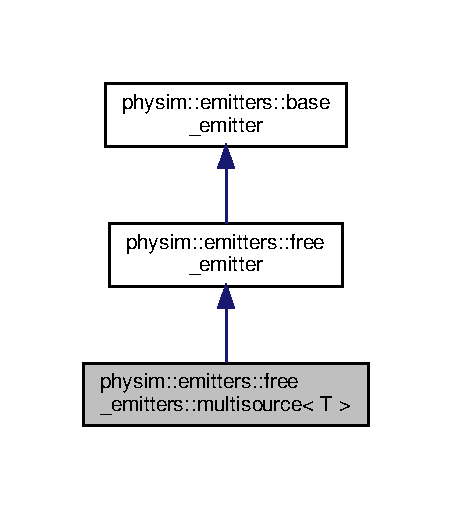
\includegraphics[width=217pt]{classphysim_1_1emitters_1_1free__emitters_1_1multisource__inherit__graph}
\end{center}
\end{figure}


Collaboration diagram for physim\+:\+:emitters\+:\+:free\+\_\+emitters\+:\+:multisource$<$ T $>$\+:\nopagebreak
\begin{figure}[H]
\begin{center}
\leavevmode
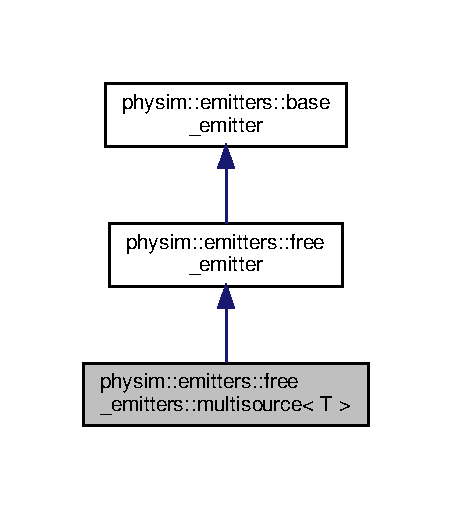
\includegraphics[width=217pt]{classphysim_1_1emitters_1_1free__emitters_1_1multisource__coll__graph}
\end{center}
\end{figure}
\subsection*{Public Member Functions}
\begin{DoxyCompactItemize}
\item 
\mbox{\Hypertarget{classphysim_1_1emitters_1_1free__emitters_1_1multisource_a43529c4f6b91b56b6b24c2b4ed97f049}\label{classphysim_1_1emitters_1_1free__emitters_1_1multisource_a43529c4f6b91b56b6b24c2b4ed97f049}} 
\hyperlink{classphysim_1_1emitters_1_1free__emitters_1_1multisource_a43529c4f6b91b56b6b24c2b4ed97f049}{multisource} ()
\begin{DoxyCompactList}\small\item\em Default constructor. \end{DoxyCompactList}\item 
\mbox{\Hypertarget{classphysim_1_1emitters_1_1free__emitters_1_1multisource_a4282f4d4c555af38eb82dcfe6383fca4}\label{classphysim_1_1emitters_1_1free__emitters_1_1multisource_a4282f4d4c555af38eb82dcfe6383fca4}} 
\hyperlink{classphysim_1_1emitters_1_1free__emitters_1_1multisource_a4282f4d4c555af38eb82dcfe6383fca4}{$\sim$multisource} ()
\begin{DoxyCompactList}\small\item\em Destructor. \end{DoxyCompactList}\item 
void \hyperlink{classphysim_1_1emitters_1_1free__emitters_1_1multisource_ab1f79cb5a7f03279dca7f6b3aa98c903}{allocate} (size\+\_\+t N, size\+\_\+t n)
\begin{DoxyCompactList}\small\item\em Allocates space for {\itshape n} initialisers. \end{DoxyCompactList}\item 
void \hyperlink{classphysim_1_1emitters_1_1free__emitters_1_1multisource_a6848d75a037d33e1b8a046f51a947c19}{use\+\_\+position\+\_\+init} (bool u=true)
\begin{DoxyCompactList}\small\item\em The position initialiser will be remade when copying. \end{DoxyCompactList}\item 
void \hyperlink{classphysim_1_1emitters_1_1free__emitters_1_1multisource_a05fbb3684dbcfdebd7daea7ccbd75cf9}{use\+\_\+velocity\+\_\+init} (bool u=true)
\begin{DoxyCompactList}\small\item\em The velocity initialiser will be remade when copying. \end{DoxyCompactList}\item 
void \hyperlink{classphysim_1_1emitters_1_1free__emitters_1_1multisource_a7fb61c1618b2e22f8afd953d065b52b8}{use\+\_\+mass\+\_\+init} (bool u=true)
\begin{DoxyCompactList}\small\item\em The mass initialiser will be remade when copying. \end{DoxyCompactList}\item 
void \hyperlink{classphysim_1_1emitters_1_1free__emitters_1_1multisource_a9def4fac2754546b0130fce7557785b3}{use\+\_\+charge\+\_\+init} (bool u=true)
\begin{DoxyCompactList}\small\item\em The charge initialiser will be remade when copying. \end{DoxyCompactList}\item 
void \hyperlink{classphysim_1_1emitters_1_1free__emitters_1_1multisource_a7953b29add1e27f1b6937ca3191d6f2f}{use\+\_\+bounce\+\_\+init} (bool u=true)
\begin{DoxyCompactList}\small\item\em The bouncing coefficient initialiser will be remade when copying. \end{DoxyCompactList}\item 
void \hyperlink{classphysim_1_1emitters_1_1free__emitters_1_1multisource_adae750ba93adee9a299e9f83735fe79e}{use\+\_\+friction\+\_\+init} (bool u=true)
\begin{DoxyCompactList}\small\item\em The friction coefficient initialiser will be remade when copying. \end{DoxyCompactList}\item 
void \hyperlink{classphysim_1_1emitters_1_1free__emitters_1_1multisource_a1e2a1b53db17d53177706d6d46884a59}{use\+\_\+lifetime\+\_\+init} (bool u=true)
\begin{DoxyCompactList}\small\item\em The lifetime initialiser will be remade when copying. \end{DoxyCompactList}\item 
void \hyperlink{classphysim_1_1emitters_1_1free__emitters_1_1multisource_a89210347706352017c867877bc16fbec}{use\+\_\+starttime\+\_\+init} (bool u=true)
\begin{DoxyCompactList}\small\item\em The starttime initialiser will be remade when copying. \end{DoxyCompactList}\item 
void \hyperlink{classphysim_1_1emitters_1_1free__emitters_1_1multisource_a115436d1054f17688925a6157399f7a9}{use\+\_\+fixed\+\_\+init} (bool u=true)
\begin{DoxyCompactList}\small\item\em The fixed attribute initialiser will be remade when copying. \end{DoxyCompactList}\item 
void \hyperlink{classphysim_1_1emitters_1_1free__emitters_1_1multisource_a733668bafd378a28fb4c83228f66da9f}{make\+\_\+position\+\_\+init} ()
\begin{DoxyCompactList}\small\item\em Make position initialiser. See \hyperlink{classphysim_1_1emitters_1_1base__emitter_ac67584a2ca34232c1f4f04c41599df0e}{free\+\_\+emitter\+::pos}. \end{DoxyCompactList}\item 
void \hyperlink{classphysim_1_1emitters_1_1free__emitters_1_1multisource_a638cc70a85d14ec5cc836f4b58611a3a}{make\+\_\+velocity\+\_\+init} ()
\begin{DoxyCompactList}\small\item\em Make velocity initialiser. See \hyperlink{classphysim_1_1emitters_1_1base__emitter_a9ea19d96450cff65882371b61a2294c8}{free\+\_\+emitter\+::vel}. \end{DoxyCompactList}\item 
void \hyperlink{classphysim_1_1emitters_1_1free__emitters_1_1multisource_aecd70362b2df41276206a600c55a78a8}{make\+\_\+mass\+\_\+init} ()
\begin{DoxyCompactList}\small\item\em Make mass initialiser. See \hyperlink{classphysim_1_1emitters_1_1base__emitter_a4e1b65730afef86899544d3306f7547d}{free\+\_\+emitter\+::mass}. \end{DoxyCompactList}\item 
void \hyperlink{classphysim_1_1emitters_1_1free__emitters_1_1multisource_adf1381635d55a57009d6e71a13c743d8}{make\+\_\+charge\+\_\+init} ()
\begin{DoxyCompactList}\small\item\em Make charge initialiser. See \hyperlink{classphysim_1_1emitters_1_1free__emitter_a895244d2023c4cc72658d356bdb51b9a}{free\+\_\+emitter\+::charge}. \end{DoxyCompactList}\item 
void \hyperlink{classphysim_1_1emitters_1_1free__emitters_1_1multisource_a0f49d5a98f7ab5be200ec471ed71258e}{make\+\_\+bounce\+\_\+init} ()
\begin{DoxyCompactList}\small\item\em Make bounce initialiser. See \hyperlink{classphysim_1_1emitters_1_1free__emitter_a71006743e284b12904d7a4b4127ab4b8}{free\+\_\+emitter\+::bounce}. \end{DoxyCompactList}\item 
void \hyperlink{classphysim_1_1emitters_1_1free__emitters_1_1multisource_ad179c7246d3fe615e327fb9866570f6f}{make\+\_\+friction\+\_\+init} ()
\begin{DoxyCompactList}\small\item\em Make friction initialiser. See \hyperlink{classphysim_1_1emitters_1_1free__emitter_a0167889dfac9483e7e2690efc353a7bd}{free\+\_\+emitter\+::friction}. \end{DoxyCompactList}\item 
void \hyperlink{classphysim_1_1emitters_1_1free__emitters_1_1multisource_a98060cb2539012355cab5179086b1535}{make\+\_\+lifetime\+\_\+init} ()
\begin{DoxyCompactList}\small\item\em Make lifetime initialiser. See \hyperlink{classphysim_1_1emitters_1_1free__emitter_a596108fe3602299fa9035ece668653d4}{free\+\_\+emitter\+::lifetime}. \end{DoxyCompactList}\item 
void \hyperlink{classphysim_1_1emitters_1_1free__emitters_1_1multisource_a2e750255e30d76c1e6ef69dec8e01d3b}{make\+\_\+starttime\+\_\+init} ()
\begin{DoxyCompactList}\small\item\em Make starttime initialiser. See \hyperlink{classphysim_1_1emitters_1_1free__emitter_af296f735438087c4acaba2242c839e49}{free\+\_\+emitter\+::starttime}. \end{DoxyCompactList}\item 
void \hyperlink{classphysim_1_1emitters_1_1free__emitters_1_1multisource_aa6fa54d4dc49b140005bf162e9b5f5b4}{make\+\_\+fixed\+\_\+init} ()
\begin{DoxyCompactList}\small\item\em Make fixed initialiser. See \hyperlink{classphysim_1_1emitters_1_1free__emitter_a2561dbe073b699e28fbb7ad10e897567}{free\+\_\+emitter\+::fixed}. \end{DoxyCompactList}\item 
\mbox{\Hypertarget{classphysim_1_1emitters_1_1free__emitters_1_1multisource_ad4ba3877c01edbfb644d60344db58933}\label{classphysim_1_1emitters_1_1free__emitters_1_1multisource_ad4ba3877c01edbfb644d60344db58933}} 
void \hyperlink{classphysim_1_1emitters_1_1free__emitters_1_1multisource_ad4ba3877c01edbfb644d60344db58933}{make\+\_\+all\+\_\+init} ()
\begin{DoxyCompactList}\small\item\em Calls all make\+\_\+$\ast$\+\_\+init functions. \end{DoxyCompactList}\item 
\mbox{\Hypertarget{classphysim_1_1emitters_1_1free__emitters_1_1multisource_a84bafdf796853c0f5546f7e092df7c02}\label{classphysim_1_1emitters_1_1free__emitters_1_1multisource_a84bafdf796853c0f5546f7e092df7c02}} 
size\+\_\+t \hyperlink{classphysim_1_1emitters_1_1free__emitters_1_1multisource_a84bafdf796853c0f5546f7e092df7c02}{size} () const
\begin{DoxyCompactList}\small\item\em Returns the amount of sources of this mutlisource emitter. \end{DoxyCompactList}\item 
\mbox{\Hypertarget{classphysim_1_1emitters_1_1free__emitters_1_1multisource_aff534fc05593b50fcf710bf87be5490c}\label{classphysim_1_1emitters_1_1free__emitters_1_1multisource_aff534fc05593b50fcf710bf87be5490c}} 
std\+::vector$<$ T $>$ \& \hyperlink{classphysim_1_1emitters_1_1free__emitters_1_1multisource_aff534fc05593b50fcf710bf87be5490c}{get\+\_\+sources} ()
\begin{DoxyCompactList}\small\item\em Returns a reference to the sources. \end{DoxyCompactList}\item 
\mbox{\Hypertarget{classphysim_1_1emitters_1_1free__emitters_1_1multisource_ae32bb527aee8a67e5aac4ea05eb88607}\label{classphysim_1_1emitters_1_1free__emitters_1_1multisource_ae32bb527aee8a67e5aac4ea05eb88607}} 
const std\+::vector$<$ T $>$ \& \hyperlink{classphysim_1_1emitters_1_1free__emitters_1_1multisource_ae32bb527aee8a67e5aac4ea05eb88607}{get\+\_\+sources} () const
\begin{DoxyCompactList}\small\item\em Returns a constant reference to the sources. \end{DoxyCompactList}\item 
\mbox{\Hypertarget{classphysim_1_1emitters_1_1free__emitters_1_1multisource_aff22e6a618f4237aa2f244cd0297fe84}\label{classphysim_1_1emitters_1_1free__emitters_1_1multisource_aff22e6a618f4237aa2f244cd0297fe84}} 
\hyperlink{classphysim_1_1emitters_1_1free__emitter}{free\+\_\+emitter} $\ast$ \hyperlink{classphysim_1_1emitters_1_1free__emitters_1_1multisource_aff22e6a618f4237aa2f244cd0297fe84}{clone} () const
\begin{DoxyCompactList}\small\item\em Returns a reference to a copy of this emitter. \end{DoxyCompactList}\end{DoxyCompactItemize}
\subsection*{Private Attributes}
\begin{DoxyCompactItemize}
\item 
\mbox{\Hypertarget{classphysim_1_1emitters_1_1free__emitters_1_1multisource_a5d7da0aee3013d8b0f498d75b6bf2e8c}\label{classphysim_1_1emitters_1_1free__emitters_1_1multisource_a5d7da0aee3013d8b0f498d75b6bf2e8c}} 
size\+\_\+t \hyperlink{classphysim_1_1emitters_1_1free__emitters_1_1multisource_a5d7da0aee3013d8b0f498d75b6bf2e8c}{P}
\begin{DoxyCompactList}\small\item\em Number of particles in the simulation. \end{DoxyCompactList}\item 
\mbox{\Hypertarget{classphysim_1_1emitters_1_1free__emitters_1_1multisource_af6304e14f12572ab5b768b0d5ec54d35}\label{classphysim_1_1emitters_1_1free__emitters_1_1multisource_af6304e14f12572ab5b768b0d5ec54d35}} 
std\+::vector$<$ T $>$ \hyperlink{classphysim_1_1emitters_1_1free__emitters_1_1multisource_af6304e14f12572ab5b768b0d5ec54d35}{sources}
\begin{DoxyCompactList}\small\item\em Collection of sources for this multiple source emitter. \end{DoxyCompactList}\item 
unsigned int \hyperlink{classphysim_1_1emitters_1_1free__emitters_1_1multisource_a99bad5ac0fb5cb14652bbfd0c1f0eeff}{use\+\_\+functions}
\begin{DoxyCompactList}\small\item\em Bit mask that indicates what functions are used. \end{DoxyCompactList}\end{DoxyCompactItemize}
\subsection*{Additional Inherited Members}


\subsection{Detailed Description}
\subsubsection*{template$<$class T$>$\newline
class physim\+::emitters\+::free\+\_\+emitters\+::multisource$<$ T $>$}

Emitter from multiple sources. 

This class implements a \hyperlink{classphysim_1_1emitters_1_1free__emitter}{free\+\_\+emitter} that uses multiple initialisers of the same type.

This can be used, for example, to have several hoses in the same simulator.

In order to achieve this, the class divides into chunks of similar size all the particles in the simulation. If there are $n$ particles in the simulation and this class has $s$ sources then every chunk will have $n/s$ particles in it. The {\itshape i-\/th} chunk is assigned the particles with index

$[i*\lfloor n/s \rfloor), (i + 1)*\lfloor n/s \rfloor)$, $[(s - 1)*\lfloor n/s \rfloor), n$

for $i \in [0,s - 2] $

Since \$ $n$ may not be a multiple of $s$ then the last chunk will have a few more particles than the others.

In particular, the last chunk will have $n - (s - 1)*\lfloor n/s \rfloor) + 1$ particles.

The sources should be set by retrieving the reference to the sources container (see \hyperlink{classphysim_1_1emitters_1_1free__emitters_1_1multisource_aff534fc05593b50fcf710bf87be5490c}{get\+\_\+sources}) after allocating the wanted amount (see \hyperlink{classphysim_1_1emitters_1_1free__emitters_1_1multisource_ab1f79cb5a7f03279dca7f6b3aa98c903}{allocate}).

Some of the functions used to initialise the chunks of particles will have to be remade in the copy constructor. The functions to be remade are indicated by calling the use\+\_\+$\ast$\+\_\+init functions. Notice that when using the \hyperlink{classphysim_1_1emitters_1_1free__emitters_1_1hose}{hose} the initialisers for the position and velocity init must be remade. 

\subsection{Member Function Documentation}
\mbox{\Hypertarget{classphysim_1_1emitters_1_1free__emitters_1_1multisource_ab1f79cb5a7f03279dca7f6b3aa98c903}\label{classphysim_1_1emitters_1_1free__emitters_1_1multisource_ab1f79cb5a7f03279dca7f6b3aa98c903}} 
\index{physim\+::emitters\+::free\+\_\+emitters\+::multisource@{physim\+::emitters\+::free\+\_\+emitters\+::multisource}!allocate@{allocate}}
\index{allocate@{allocate}!physim\+::emitters\+::free\+\_\+emitters\+::multisource@{physim\+::emitters\+::free\+\_\+emitters\+::multisource}}
\subsubsection{\texorpdfstring{allocate()}{allocate()}}
{\footnotesize\ttfamily template$<$class T $>$ \\
void \hyperlink{classphysim_1_1emitters_1_1free__emitters_1_1multisource}{physim\+::emitters\+::free\+\_\+emitters\+::multisource}$<$ T $>$\+::allocate (\begin{DoxyParamCaption}\item[{size\+\_\+t}]{N,  }\item[{size\+\_\+t}]{n }\end{DoxyParamCaption})}



Allocates space for {\itshape n} initialisers. 

Resizes \hyperlink{classphysim_1_1emitters_1_1free__emitters_1_1multisource_af6304e14f12572ab5b768b0d5ec54d35}{sources} to have {\itshape n} elements. 
\begin{DoxyParams}{Parameters}
{\em N} & Number of particles in the simulation. \\
\hline
{\em n} & Number of initialisers. \\
\hline
\end{DoxyParams}
\mbox{\Hypertarget{classphysim_1_1emitters_1_1free__emitters_1_1multisource_a0f49d5a98f7ab5be200ec471ed71258e}\label{classphysim_1_1emitters_1_1free__emitters_1_1multisource_a0f49d5a98f7ab5be200ec471ed71258e}} 
\index{physim\+::emitters\+::free\+\_\+emitters\+::multisource@{physim\+::emitters\+::free\+\_\+emitters\+::multisource}!make\+\_\+bounce\+\_\+init@{make\+\_\+bounce\+\_\+init}}
\index{make\+\_\+bounce\+\_\+init@{make\+\_\+bounce\+\_\+init}!physim\+::emitters\+::free\+\_\+emitters\+::multisource@{physim\+::emitters\+::free\+\_\+emitters\+::multisource}}
\subsubsection{\texorpdfstring{make\+\_\+bounce\+\_\+init()}{make\_bounce\_init()}}
{\footnotesize\ttfamily template$<$class T $>$ \\
void \hyperlink{classphysim_1_1emitters_1_1free__emitters_1_1multisource}{physim\+::emitters\+::free\+\_\+emitters\+::multisource}$<$ T $>$\+::make\+\_\+bounce\+\_\+init (\begin{DoxyParamCaption}{ }\end{DoxyParamCaption})}



Make bounce initialiser. See \hyperlink{classphysim_1_1emitters_1_1free__emitter_a71006743e284b12904d7a4b4127ab4b8}{free\+\_\+emitter\+::bounce}. 

The {\itshape i-\/th} particle is assigned its bouncing coefficient using the {\itshape k-\/th} source. See description of the class for details on what source is used. \mbox{\Hypertarget{classphysim_1_1emitters_1_1free__emitters_1_1multisource_adf1381635d55a57009d6e71a13c743d8}\label{classphysim_1_1emitters_1_1free__emitters_1_1multisource_adf1381635d55a57009d6e71a13c743d8}} 
\index{physim\+::emitters\+::free\+\_\+emitters\+::multisource@{physim\+::emitters\+::free\+\_\+emitters\+::multisource}!make\+\_\+charge\+\_\+init@{make\+\_\+charge\+\_\+init}}
\index{make\+\_\+charge\+\_\+init@{make\+\_\+charge\+\_\+init}!physim\+::emitters\+::free\+\_\+emitters\+::multisource@{physim\+::emitters\+::free\+\_\+emitters\+::multisource}}
\subsubsection{\texorpdfstring{make\+\_\+charge\+\_\+init()}{make\_charge\_init()}}
{\footnotesize\ttfamily template$<$class T $>$ \\
void \hyperlink{classphysim_1_1emitters_1_1free__emitters_1_1multisource}{physim\+::emitters\+::free\+\_\+emitters\+::multisource}$<$ T $>$\+::make\+\_\+charge\+\_\+init (\begin{DoxyParamCaption}{ }\end{DoxyParamCaption})}



Make charge initialiser. See \hyperlink{classphysim_1_1emitters_1_1free__emitter_a895244d2023c4cc72658d356bdb51b9a}{free\+\_\+emitter\+::charge}. 

The {\itshape i-\/th} particle is assigned its charge using the {\itshape k-\/th} source. See description of the class for details on what source is used. \mbox{\Hypertarget{classphysim_1_1emitters_1_1free__emitters_1_1multisource_aa6fa54d4dc49b140005bf162e9b5f5b4}\label{classphysim_1_1emitters_1_1free__emitters_1_1multisource_aa6fa54d4dc49b140005bf162e9b5f5b4}} 
\index{physim\+::emitters\+::free\+\_\+emitters\+::multisource@{physim\+::emitters\+::free\+\_\+emitters\+::multisource}!make\+\_\+fixed\+\_\+init@{make\+\_\+fixed\+\_\+init}}
\index{make\+\_\+fixed\+\_\+init@{make\+\_\+fixed\+\_\+init}!physim\+::emitters\+::free\+\_\+emitters\+::multisource@{physim\+::emitters\+::free\+\_\+emitters\+::multisource}}
\subsubsection{\texorpdfstring{make\+\_\+fixed\+\_\+init()}{make\_fixed\_init()}}
{\footnotesize\ttfamily template$<$class T $>$ \\
void \hyperlink{classphysim_1_1emitters_1_1free__emitters_1_1multisource}{physim\+::emitters\+::free\+\_\+emitters\+::multisource}$<$ T $>$\+::make\+\_\+fixed\+\_\+init (\begin{DoxyParamCaption}{ }\end{DoxyParamCaption})}



Make fixed initialiser. See \hyperlink{classphysim_1_1emitters_1_1free__emitter_a2561dbe073b699e28fbb7ad10e897567}{free\+\_\+emitter\+::fixed}. 

The {\itshape i-\/th} particle is assigned its \textquotesingle{}fixed\textquotesingle{} attribute using the {\itshape k-\/th} source. See description of the class for details on what source is used. \mbox{\Hypertarget{classphysim_1_1emitters_1_1free__emitters_1_1multisource_ad179c7246d3fe615e327fb9866570f6f}\label{classphysim_1_1emitters_1_1free__emitters_1_1multisource_ad179c7246d3fe615e327fb9866570f6f}} 
\index{physim\+::emitters\+::free\+\_\+emitters\+::multisource@{physim\+::emitters\+::free\+\_\+emitters\+::multisource}!make\+\_\+friction\+\_\+init@{make\+\_\+friction\+\_\+init}}
\index{make\+\_\+friction\+\_\+init@{make\+\_\+friction\+\_\+init}!physim\+::emitters\+::free\+\_\+emitters\+::multisource@{physim\+::emitters\+::free\+\_\+emitters\+::multisource}}
\subsubsection{\texorpdfstring{make\+\_\+friction\+\_\+init()}{make\_friction\_init()}}
{\footnotesize\ttfamily template$<$class T $>$ \\
void \hyperlink{classphysim_1_1emitters_1_1free__emitters_1_1multisource}{physim\+::emitters\+::free\+\_\+emitters\+::multisource}$<$ T $>$\+::make\+\_\+friction\+\_\+init (\begin{DoxyParamCaption}{ }\end{DoxyParamCaption})}



Make friction initialiser. See \hyperlink{classphysim_1_1emitters_1_1free__emitter_a0167889dfac9483e7e2690efc353a7bd}{free\+\_\+emitter\+::friction}. 

The {\itshape i-\/th} particle is assigned its position using the {\itshape k-\/th} source. See description of the class for details on what source is used. \mbox{\Hypertarget{classphysim_1_1emitters_1_1free__emitters_1_1multisource_a98060cb2539012355cab5179086b1535}\label{classphysim_1_1emitters_1_1free__emitters_1_1multisource_a98060cb2539012355cab5179086b1535}} 
\index{physim\+::emitters\+::free\+\_\+emitters\+::multisource@{physim\+::emitters\+::free\+\_\+emitters\+::multisource}!make\+\_\+lifetime\+\_\+init@{make\+\_\+lifetime\+\_\+init}}
\index{make\+\_\+lifetime\+\_\+init@{make\+\_\+lifetime\+\_\+init}!physim\+::emitters\+::free\+\_\+emitters\+::multisource@{physim\+::emitters\+::free\+\_\+emitters\+::multisource}}
\subsubsection{\texorpdfstring{make\+\_\+lifetime\+\_\+init()}{make\_lifetime\_init()}}
{\footnotesize\ttfamily template$<$class T $>$ \\
void \hyperlink{classphysim_1_1emitters_1_1free__emitters_1_1multisource}{physim\+::emitters\+::free\+\_\+emitters\+::multisource}$<$ T $>$\+::make\+\_\+lifetime\+\_\+init (\begin{DoxyParamCaption}{ }\end{DoxyParamCaption})}



Make lifetime initialiser. See \hyperlink{classphysim_1_1emitters_1_1free__emitter_a596108fe3602299fa9035ece668653d4}{free\+\_\+emitter\+::lifetime}. 

The {\itshape i-\/th} particle is assigned its lifetime using the {\itshape k-\/th} source. See description of the class for details on what source is used. \mbox{\Hypertarget{classphysim_1_1emitters_1_1free__emitters_1_1multisource_aecd70362b2df41276206a600c55a78a8}\label{classphysim_1_1emitters_1_1free__emitters_1_1multisource_aecd70362b2df41276206a600c55a78a8}} 
\index{physim\+::emitters\+::free\+\_\+emitters\+::multisource@{physim\+::emitters\+::free\+\_\+emitters\+::multisource}!make\+\_\+mass\+\_\+init@{make\+\_\+mass\+\_\+init}}
\index{make\+\_\+mass\+\_\+init@{make\+\_\+mass\+\_\+init}!physim\+::emitters\+::free\+\_\+emitters\+::multisource@{physim\+::emitters\+::free\+\_\+emitters\+::multisource}}
\subsubsection{\texorpdfstring{make\+\_\+mass\+\_\+init()}{make\_mass\_init()}}
{\footnotesize\ttfamily template$<$class T $>$ \\
void \hyperlink{classphysim_1_1emitters_1_1free__emitters_1_1multisource}{physim\+::emitters\+::free\+\_\+emitters\+::multisource}$<$ T $>$\+::make\+\_\+mass\+\_\+init (\begin{DoxyParamCaption}{ }\end{DoxyParamCaption})}



Make mass initialiser. See \hyperlink{classphysim_1_1emitters_1_1base__emitter_a4e1b65730afef86899544d3306f7547d}{free\+\_\+emitter\+::mass}. 

The {\itshape i-\/th} particle is assigned its mass using the {\itshape k-\/th} source. See description of the class for details on what source is used. \mbox{\Hypertarget{classphysim_1_1emitters_1_1free__emitters_1_1multisource_a733668bafd378a28fb4c83228f66da9f}\label{classphysim_1_1emitters_1_1free__emitters_1_1multisource_a733668bafd378a28fb4c83228f66da9f}} 
\index{physim\+::emitters\+::free\+\_\+emitters\+::multisource@{physim\+::emitters\+::free\+\_\+emitters\+::multisource}!make\+\_\+position\+\_\+init@{make\+\_\+position\+\_\+init}}
\index{make\+\_\+position\+\_\+init@{make\+\_\+position\+\_\+init}!physim\+::emitters\+::free\+\_\+emitters\+::multisource@{physim\+::emitters\+::free\+\_\+emitters\+::multisource}}
\subsubsection{\texorpdfstring{make\+\_\+position\+\_\+init()}{make\_position\_init()}}
{\footnotesize\ttfamily template$<$class T $>$ \\
void \hyperlink{classphysim_1_1emitters_1_1free__emitters_1_1multisource}{physim\+::emitters\+::free\+\_\+emitters\+::multisource}$<$ T $>$\+::make\+\_\+position\+\_\+init (\begin{DoxyParamCaption}{ }\end{DoxyParamCaption})}



Make position initialiser. See \hyperlink{classphysim_1_1emitters_1_1base__emitter_ac67584a2ca34232c1f4f04c41599df0e}{free\+\_\+emitter\+::pos}. 

The {\itshape i-\/th} particle is assigned its position using the {\itshape k-\/th} source. See description of the class for details on what source is used. \mbox{\Hypertarget{classphysim_1_1emitters_1_1free__emitters_1_1multisource_a2e750255e30d76c1e6ef69dec8e01d3b}\label{classphysim_1_1emitters_1_1free__emitters_1_1multisource_a2e750255e30d76c1e6ef69dec8e01d3b}} 
\index{physim\+::emitters\+::free\+\_\+emitters\+::multisource@{physim\+::emitters\+::free\+\_\+emitters\+::multisource}!make\+\_\+starttime\+\_\+init@{make\+\_\+starttime\+\_\+init}}
\index{make\+\_\+starttime\+\_\+init@{make\+\_\+starttime\+\_\+init}!physim\+::emitters\+::free\+\_\+emitters\+::multisource@{physim\+::emitters\+::free\+\_\+emitters\+::multisource}}
\subsubsection{\texorpdfstring{make\+\_\+starttime\+\_\+init()}{make\_starttime\_init()}}
{\footnotesize\ttfamily template$<$class T $>$ \\
void \hyperlink{classphysim_1_1emitters_1_1free__emitters_1_1multisource}{physim\+::emitters\+::free\+\_\+emitters\+::multisource}$<$ T $>$\+::make\+\_\+starttime\+\_\+init (\begin{DoxyParamCaption}{ }\end{DoxyParamCaption})}



Make starttime initialiser. See \hyperlink{classphysim_1_1emitters_1_1free__emitter_af296f735438087c4acaba2242c839e49}{free\+\_\+emitter\+::starttime}. 

The {\itshape i-\/th} particle is assigned its starttime using the {\itshape k-\/th} source. See description of the class for details on what source is used. \mbox{\Hypertarget{classphysim_1_1emitters_1_1free__emitters_1_1multisource_a638cc70a85d14ec5cc836f4b58611a3a}\label{classphysim_1_1emitters_1_1free__emitters_1_1multisource_a638cc70a85d14ec5cc836f4b58611a3a}} 
\index{physim\+::emitters\+::free\+\_\+emitters\+::multisource@{physim\+::emitters\+::free\+\_\+emitters\+::multisource}!make\+\_\+velocity\+\_\+init@{make\+\_\+velocity\+\_\+init}}
\index{make\+\_\+velocity\+\_\+init@{make\+\_\+velocity\+\_\+init}!physim\+::emitters\+::free\+\_\+emitters\+::multisource@{physim\+::emitters\+::free\+\_\+emitters\+::multisource}}
\subsubsection{\texorpdfstring{make\+\_\+velocity\+\_\+init()}{make\_velocity\_init()}}
{\footnotesize\ttfamily template$<$class T $>$ \\
void \hyperlink{classphysim_1_1emitters_1_1free__emitters_1_1multisource}{physim\+::emitters\+::free\+\_\+emitters\+::multisource}$<$ T $>$\+::make\+\_\+velocity\+\_\+init (\begin{DoxyParamCaption}{ }\end{DoxyParamCaption})}



Make velocity initialiser. See \hyperlink{classphysim_1_1emitters_1_1base__emitter_a9ea19d96450cff65882371b61a2294c8}{free\+\_\+emitter\+::vel}. 

The {\itshape i-\/th} particle is assigned its velocity using the {\itshape k-\/th} source. See description of the class for details on what source is used. \mbox{\Hypertarget{classphysim_1_1emitters_1_1free__emitters_1_1multisource_a7953b29add1e27f1b6937ca3191d6f2f}\label{classphysim_1_1emitters_1_1free__emitters_1_1multisource_a7953b29add1e27f1b6937ca3191d6f2f}} 
\index{physim\+::emitters\+::free\+\_\+emitters\+::multisource@{physim\+::emitters\+::free\+\_\+emitters\+::multisource}!use\+\_\+bounce\+\_\+init@{use\+\_\+bounce\+\_\+init}}
\index{use\+\_\+bounce\+\_\+init@{use\+\_\+bounce\+\_\+init}!physim\+::emitters\+::free\+\_\+emitters\+::multisource@{physim\+::emitters\+::free\+\_\+emitters\+::multisource}}
\subsubsection{\texorpdfstring{use\+\_\+bounce\+\_\+init()}{use\_bounce\_init()}}
{\footnotesize\ttfamily template$<$class T $>$ \\
void \hyperlink{classphysim_1_1emitters_1_1free__emitters_1_1multisource}{physim\+::emitters\+::free\+\_\+emitters\+::multisource}$<$ T $>$\+::use\+\_\+bounce\+\_\+init (\begin{DoxyParamCaption}\item[{bool}]{u = {\ttfamily true} }\end{DoxyParamCaption})}



The bouncing coefficient initialiser will be remade when copying. 

Sets or unsets the 4 bit of \hyperlink{classphysim_1_1emitters_1_1free__emitters_1_1multisource_a99bad5ac0fb5cb14652bbfd0c1f0eeff}{use\+\_\+functions}; 
\begin{DoxyParams}{Parameters}
{\em u} & Either true or false. \\
\hline
\end{DoxyParams}
\mbox{\Hypertarget{classphysim_1_1emitters_1_1free__emitters_1_1multisource_a9def4fac2754546b0130fce7557785b3}\label{classphysim_1_1emitters_1_1free__emitters_1_1multisource_a9def4fac2754546b0130fce7557785b3}} 
\index{physim\+::emitters\+::free\+\_\+emitters\+::multisource@{physim\+::emitters\+::free\+\_\+emitters\+::multisource}!use\+\_\+charge\+\_\+init@{use\+\_\+charge\+\_\+init}}
\index{use\+\_\+charge\+\_\+init@{use\+\_\+charge\+\_\+init}!physim\+::emitters\+::free\+\_\+emitters\+::multisource@{physim\+::emitters\+::free\+\_\+emitters\+::multisource}}
\subsubsection{\texorpdfstring{use\+\_\+charge\+\_\+init()}{use\_charge\_init()}}
{\footnotesize\ttfamily template$<$class T $>$ \\
void \hyperlink{classphysim_1_1emitters_1_1free__emitters_1_1multisource}{physim\+::emitters\+::free\+\_\+emitters\+::multisource}$<$ T $>$\+::use\+\_\+charge\+\_\+init (\begin{DoxyParamCaption}\item[{bool}]{u = {\ttfamily true} }\end{DoxyParamCaption})}



The charge initialiser will be remade when copying. 

Sets or unsets the 3 bit of \hyperlink{classphysim_1_1emitters_1_1free__emitters_1_1multisource_a99bad5ac0fb5cb14652bbfd0c1f0eeff}{use\+\_\+functions}; 
\begin{DoxyParams}{Parameters}
{\em u} & Either true or false. \\
\hline
\end{DoxyParams}
\mbox{\Hypertarget{classphysim_1_1emitters_1_1free__emitters_1_1multisource_a115436d1054f17688925a6157399f7a9}\label{classphysim_1_1emitters_1_1free__emitters_1_1multisource_a115436d1054f17688925a6157399f7a9}} 
\index{physim\+::emitters\+::free\+\_\+emitters\+::multisource@{physim\+::emitters\+::free\+\_\+emitters\+::multisource}!use\+\_\+fixed\+\_\+init@{use\+\_\+fixed\+\_\+init}}
\index{use\+\_\+fixed\+\_\+init@{use\+\_\+fixed\+\_\+init}!physim\+::emitters\+::free\+\_\+emitters\+::multisource@{physim\+::emitters\+::free\+\_\+emitters\+::multisource}}
\subsubsection{\texorpdfstring{use\+\_\+fixed\+\_\+init()}{use\_fixed\_init()}}
{\footnotesize\ttfamily template$<$class T $>$ \\
void \hyperlink{classphysim_1_1emitters_1_1free__emitters_1_1multisource}{physim\+::emitters\+::free\+\_\+emitters\+::multisource}$<$ T $>$\+::use\+\_\+fixed\+\_\+init (\begin{DoxyParamCaption}\item[{bool}]{u = {\ttfamily true} }\end{DoxyParamCaption})}



The fixed attribute initialiser will be remade when copying. 

Sets or unsets the 8 bit of \hyperlink{classphysim_1_1emitters_1_1free__emitters_1_1multisource_a99bad5ac0fb5cb14652bbfd0c1f0eeff}{use\+\_\+functions}; 
\begin{DoxyParams}{Parameters}
{\em u} & Either true or false. \\
\hline
\end{DoxyParams}
\mbox{\Hypertarget{classphysim_1_1emitters_1_1free__emitters_1_1multisource_adae750ba93adee9a299e9f83735fe79e}\label{classphysim_1_1emitters_1_1free__emitters_1_1multisource_adae750ba93adee9a299e9f83735fe79e}} 
\index{physim\+::emitters\+::free\+\_\+emitters\+::multisource@{physim\+::emitters\+::free\+\_\+emitters\+::multisource}!use\+\_\+friction\+\_\+init@{use\+\_\+friction\+\_\+init}}
\index{use\+\_\+friction\+\_\+init@{use\+\_\+friction\+\_\+init}!physim\+::emitters\+::free\+\_\+emitters\+::multisource@{physim\+::emitters\+::free\+\_\+emitters\+::multisource}}
\subsubsection{\texorpdfstring{use\+\_\+friction\+\_\+init()}{use\_friction\_init()}}
{\footnotesize\ttfamily template$<$class T $>$ \\
void \hyperlink{classphysim_1_1emitters_1_1free__emitters_1_1multisource}{physim\+::emitters\+::free\+\_\+emitters\+::multisource}$<$ T $>$\+::use\+\_\+friction\+\_\+init (\begin{DoxyParamCaption}\item[{bool}]{u = {\ttfamily true} }\end{DoxyParamCaption})}



The friction coefficient initialiser will be remade when copying. 

Sets or unsets the 5 bit of \hyperlink{classphysim_1_1emitters_1_1free__emitters_1_1multisource_a99bad5ac0fb5cb14652bbfd0c1f0eeff}{use\+\_\+functions}; 
\begin{DoxyParams}{Parameters}
{\em u} & Either true or false. \\
\hline
\end{DoxyParams}
\mbox{\Hypertarget{classphysim_1_1emitters_1_1free__emitters_1_1multisource_a1e2a1b53db17d53177706d6d46884a59}\label{classphysim_1_1emitters_1_1free__emitters_1_1multisource_a1e2a1b53db17d53177706d6d46884a59}} 
\index{physim\+::emitters\+::free\+\_\+emitters\+::multisource@{physim\+::emitters\+::free\+\_\+emitters\+::multisource}!use\+\_\+lifetime\+\_\+init@{use\+\_\+lifetime\+\_\+init}}
\index{use\+\_\+lifetime\+\_\+init@{use\+\_\+lifetime\+\_\+init}!physim\+::emitters\+::free\+\_\+emitters\+::multisource@{physim\+::emitters\+::free\+\_\+emitters\+::multisource}}
\subsubsection{\texorpdfstring{use\+\_\+lifetime\+\_\+init()}{use\_lifetime\_init()}}
{\footnotesize\ttfamily template$<$class T $>$ \\
void \hyperlink{classphysim_1_1emitters_1_1free__emitters_1_1multisource}{physim\+::emitters\+::free\+\_\+emitters\+::multisource}$<$ T $>$\+::use\+\_\+lifetime\+\_\+init (\begin{DoxyParamCaption}\item[{bool}]{u = {\ttfamily true} }\end{DoxyParamCaption})}



The lifetime initialiser will be remade when copying. 

Sets or unsets the 6 bit of \hyperlink{classphysim_1_1emitters_1_1free__emitters_1_1multisource_a99bad5ac0fb5cb14652bbfd0c1f0eeff}{use\+\_\+functions}; 
\begin{DoxyParams}{Parameters}
{\em u} & Either true or false. \\
\hline
\end{DoxyParams}
\mbox{\Hypertarget{classphysim_1_1emitters_1_1free__emitters_1_1multisource_a7fb61c1618b2e22f8afd953d065b52b8}\label{classphysim_1_1emitters_1_1free__emitters_1_1multisource_a7fb61c1618b2e22f8afd953d065b52b8}} 
\index{physim\+::emitters\+::free\+\_\+emitters\+::multisource@{physim\+::emitters\+::free\+\_\+emitters\+::multisource}!use\+\_\+mass\+\_\+init@{use\+\_\+mass\+\_\+init}}
\index{use\+\_\+mass\+\_\+init@{use\+\_\+mass\+\_\+init}!physim\+::emitters\+::free\+\_\+emitters\+::multisource@{physim\+::emitters\+::free\+\_\+emitters\+::multisource}}
\subsubsection{\texorpdfstring{use\+\_\+mass\+\_\+init()}{use\_mass\_init()}}
{\footnotesize\ttfamily template$<$class T $>$ \\
void \hyperlink{classphysim_1_1emitters_1_1free__emitters_1_1multisource}{physim\+::emitters\+::free\+\_\+emitters\+::multisource}$<$ T $>$\+::use\+\_\+mass\+\_\+init (\begin{DoxyParamCaption}\item[{bool}]{u = {\ttfamily true} }\end{DoxyParamCaption})}



The mass initialiser will be remade when copying. 

Sets or unsets the 2 bit of \hyperlink{classphysim_1_1emitters_1_1free__emitters_1_1multisource_a99bad5ac0fb5cb14652bbfd0c1f0eeff}{use\+\_\+functions}; 
\begin{DoxyParams}{Parameters}
{\em u} & Either true or false. \\
\hline
\end{DoxyParams}
\mbox{\Hypertarget{classphysim_1_1emitters_1_1free__emitters_1_1multisource_a6848d75a037d33e1b8a046f51a947c19}\label{classphysim_1_1emitters_1_1free__emitters_1_1multisource_a6848d75a037d33e1b8a046f51a947c19}} 
\index{physim\+::emitters\+::free\+\_\+emitters\+::multisource@{physim\+::emitters\+::free\+\_\+emitters\+::multisource}!use\+\_\+position\+\_\+init@{use\+\_\+position\+\_\+init}}
\index{use\+\_\+position\+\_\+init@{use\+\_\+position\+\_\+init}!physim\+::emitters\+::free\+\_\+emitters\+::multisource@{physim\+::emitters\+::free\+\_\+emitters\+::multisource}}
\subsubsection{\texorpdfstring{use\+\_\+position\+\_\+init()}{use\_position\_init()}}
{\footnotesize\ttfamily template$<$class T $>$ \\
void \hyperlink{classphysim_1_1emitters_1_1free__emitters_1_1multisource}{physim\+::emitters\+::free\+\_\+emitters\+::multisource}$<$ T $>$\+::use\+\_\+position\+\_\+init (\begin{DoxyParamCaption}\item[{bool}]{u = {\ttfamily true} }\end{DoxyParamCaption})}



The position initialiser will be remade when copying. 

Sets or unsets the 0 bit of \hyperlink{classphysim_1_1emitters_1_1free__emitters_1_1multisource_a99bad5ac0fb5cb14652bbfd0c1f0eeff}{use\+\_\+functions}; 
\begin{DoxyParams}{Parameters}
{\em u} & Either true or false. \\
\hline
\end{DoxyParams}
\mbox{\Hypertarget{classphysim_1_1emitters_1_1free__emitters_1_1multisource_a89210347706352017c867877bc16fbec}\label{classphysim_1_1emitters_1_1free__emitters_1_1multisource_a89210347706352017c867877bc16fbec}} 
\index{physim\+::emitters\+::free\+\_\+emitters\+::multisource@{physim\+::emitters\+::free\+\_\+emitters\+::multisource}!use\+\_\+starttime\+\_\+init@{use\+\_\+starttime\+\_\+init}}
\index{use\+\_\+starttime\+\_\+init@{use\+\_\+starttime\+\_\+init}!physim\+::emitters\+::free\+\_\+emitters\+::multisource@{physim\+::emitters\+::free\+\_\+emitters\+::multisource}}
\subsubsection{\texorpdfstring{use\+\_\+starttime\+\_\+init()}{use\_starttime\_init()}}
{\footnotesize\ttfamily template$<$class T $>$ \\
void \hyperlink{classphysim_1_1emitters_1_1free__emitters_1_1multisource}{physim\+::emitters\+::free\+\_\+emitters\+::multisource}$<$ T $>$\+::use\+\_\+starttime\+\_\+init (\begin{DoxyParamCaption}\item[{bool}]{u = {\ttfamily true} }\end{DoxyParamCaption})}



The starttime initialiser will be remade when copying. 

Sets or unsets the 7 bit of \hyperlink{classphysim_1_1emitters_1_1free__emitters_1_1multisource_a99bad5ac0fb5cb14652bbfd0c1f0eeff}{use\+\_\+functions}; 
\begin{DoxyParams}{Parameters}
{\em u} & Either true or false. \\
\hline
\end{DoxyParams}
\mbox{\Hypertarget{classphysim_1_1emitters_1_1free__emitters_1_1multisource_a05fbb3684dbcfdebd7daea7ccbd75cf9}\label{classphysim_1_1emitters_1_1free__emitters_1_1multisource_a05fbb3684dbcfdebd7daea7ccbd75cf9}} 
\index{physim\+::emitters\+::free\+\_\+emitters\+::multisource@{physim\+::emitters\+::free\+\_\+emitters\+::multisource}!use\+\_\+velocity\+\_\+init@{use\+\_\+velocity\+\_\+init}}
\index{use\+\_\+velocity\+\_\+init@{use\+\_\+velocity\+\_\+init}!physim\+::emitters\+::free\+\_\+emitters\+::multisource@{physim\+::emitters\+::free\+\_\+emitters\+::multisource}}
\subsubsection{\texorpdfstring{use\+\_\+velocity\+\_\+init()}{use\_velocity\_init()}}
{\footnotesize\ttfamily template$<$class T $>$ \\
void \hyperlink{classphysim_1_1emitters_1_1free__emitters_1_1multisource}{physim\+::emitters\+::free\+\_\+emitters\+::multisource}$<$ T $>$\+::use\+\_\+velocity\+\_\+init (\begin{DoxyParamCaption}\item[{bool}]{u = {\ttfamily true} }\end{DoxyParamCaption})}



The velocity initialiser will be remade when copying. 

Sets or unsets the 1 bit of \hyperlink{classphysim_1_1emitters_1_1free__emitters_1_1multisource_a99bad5ac0fb5cb14652bbfd0c1f0eeff}{use\+\_\+functions}; 
\begin{DoxyParams}{Parameters}
{\em u} & Either true or false. \\
\hline
\end{DoxyParams}


\subsection{Member Data Documentation}
\mbox{\Hypertarget{classphysim_1_1emitters_1_1free__emitters_1_1multisource_a99bad5ac0fb5cb14652bbfd0c1f0eeff}\label{classphysim_1_1emitters_1_1free__emitters_1_1multisource_a99bad5ac0fb5cb14652bbfd0c1f0eeff}} 
\index{physim\+::emitters\+::free\+\_\+emitters\+::multisource@{physim\+::emitters\+::free\+\_\+emitters\+::multisource}!use\+\_\+functions@{use\+\_\+functions}}
\index{use\+\_\+functions@{use\+\_\+functions}!physim\+::emitters\+::free\+\_\+emitters\+::multisource@{physim\+::emitters\+::free\+\_\+emitters\+::multisource}}
\subsubsection{\texorpdfstring{use\+\_\+functions}{use\_functions}}
{\footnotesize\ttfamily template$<$class T $>$ \\
unsigned int \hyperlink{classphysim_1_1emitters_1_1free__emitters_1_1multisource}{physim\+::emitters\+::free\+\_\+emitters\+::multisource}$<$ T $>$\+::use\+\_\+functions\hspace{0.3cm}{\ttfamily [private]}}



Bit mask that indicates what functions are used. 

When copy-\/constructing an object of this type, some functions will have to be remade (using the appropriate make\+\_\+$\ast$\+\_\+init functions).

The least-\/weight bits of this integer represent the 9 functions available. If any of these 9 bits is set to one, then the corresponding function will be made. 

The documentation for this class was generated from the following files\+:\begin{DoxyCompactItemize}
\item 
physim/emitter/free\+\_\+emitters/multisource.\+hpp\item 
physim/emitter/free\+\_\+emitters/multisource.\+cpp\end{DoxyCompactItemize}

\hypertarget{classphysim_1_1fluids_1_1newtonian}{}\section{physim\+:\+:fluids\+:\+:newtonian Class Reference}
\label{classphysim_1_1fluids_1_1newtonian}\index{physim\+::fluids\+::newtonian@{physim\+::fluids\+::newtonian}}


Class implementing a newtonian fluid.  




{\ttfamily \#include $<$newtonian.\+hpp$>$}



Inheritance diagram for physim\+:\+:fluids\+:\+:newtonian\+:\nopagebreak
\begin{figure}[H]
\begin{center}
\leavevmode
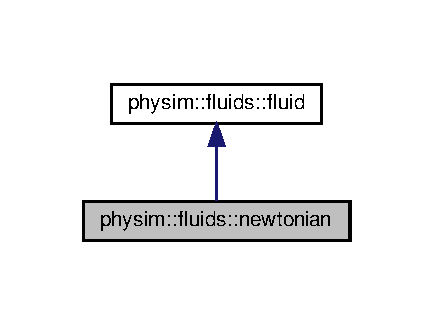
\includegraphics[width=208pt]{classphysim_1_1fluids_1_1newtonian__inherit__graph}
\end{center}
\end{figure}


Collaboration diagram for physim\+:\+:fluids\+:\+:newtonian\+:\nopagebreak
\begin{figure}[H]
\begin{center}
\leavevmode
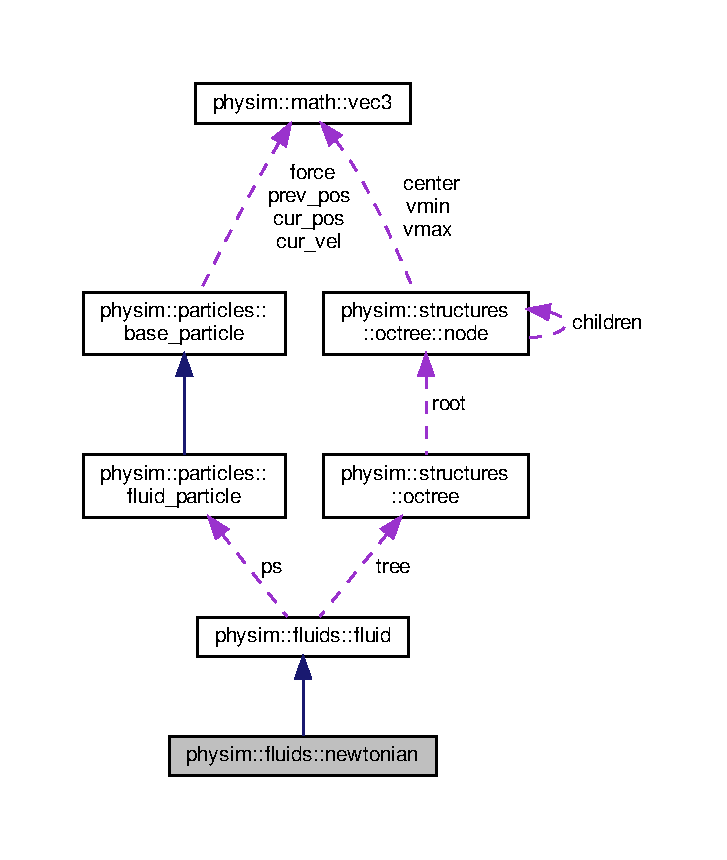
\includegraphics[width=349pt]{classphysim_1_1fluids_1_1newtonian__coll__graph}
\end{center}
\end{figure}
\subsection*{Public Member Functions}
\begin{DoxyCompactItemize}
\item 
\mbox{\Hypertarget{classphysim_1_1fluids_1_1newtonian_a4a08503213e230d59e56a42fa221d676}\label{classphysim_1_1fluids_1_1newtonian_a4a08503213e230d59e56a42fa221d676}} 
\hyperlink{classphysim_1_1fluids_1_1newtonian_a4a08503213e230d59e56a42fa221d676}{newtonian} ()
\begin{DoxyCompactList}\small\item\em Default onstructor. \end{DoxyCompactList}\item 
\mbox{\Hypertarget{classphysim_1_1fluids_1_1newtonian_a460303778bb2ecb7fd0dbed6f9988422}\label{classphysim_1_1fluids_1_1newtonian_a460303778bb2ecb7fd0dbed6f9988422}} 
virtual \hyperlink{classphysim_1_1fluids_1_1newtonian_a460303778bb2ecb7fd0dbed6f9988422}{$\sim$newtonian} ()
\begin{DoxyCompactList}\small\item\em Destructor. \end{DoxyCompactList}\item 
virtual void \hyperlink{classphysim_1_1fluids_1_1newtonian_accfe7d69d2d3985e8ec8c8179a6cf5ba}{update\+\_\+forces} ()
\begin{DoxyCompactList}\small\item\em Update the forces generated within the fluid. \end{DoxyCompactList}\item 
virtual void \hyperlink{classphysim_1_1fluids_1_1newtonian_a2ad3a26c489e0167f16cc4cd2ead981d}{update\+\_\+forces} (size\+\_\+t n)
\begin{DoxyCompactList}\small\item\em Update the forces generated within the fluid. \end{DoxyCompactList}\end{DoxyCompactItemize}
\subsection*{Additional Inherited Members}


\subsection{Detailed Description}
Class implementing a newtonian fluid. 

\subsection{Member Function Documentation}
\mbox{\Hypertarget{classphysim_1_1fluids_1_1newtonian_accfe7d69d2d3985e8ec8c8179a6cf5ba}\label{classphysim_1_1fluids_1_1newtonian_accfe7d69d2d3985e8ec8c8179a6cf5ba}} 
\index{physim\+::fluids\+::newtonian@{physim\+::fluids\+::newtonian}!update\+\_\+forces@{update\+\_\+forces}}
\index{update\+\_\+forces@{update\+\_\+forces}!physim\+::fluids\+::newtonian@{physim\+::fluids\+::newtonian}}
\subsubsection{\texorpdfstring{update\+\_\+forces()}{update\_forces()}\hspace{0.1cm}{\footnotesize\ttfamily [1/2]}}
{\footnotesize\ttfamily void physim\+::fluids\+::newtonian\+::update\+\_\+forces (\begin{DoxyParamCaption}{ }\end{DoxyParamCaption})\hspace{0.3cm}{\ttfamily [virtual]}}



Update the forces generated within the fluid. 

This method updates the forces acting on all particles. This update depends on the neighbouring information determined by the kernel functions.

This method does not update positions or velocities.

\begin{DoxyPrecond}{Precondition}
The modification of a particles\textquotesingle{} force may assume that all particles start with null force (force equal to 0 in the three axes). 

This method is called before computing the forces acting on the particles due to force fields. 
\end{DoxyPrecond}


Implements \hyperlink{classphysim_1_1fluids_1_1fluid_a6cde063d44b1e33199c08e64d801bb04}{physim\+::fluids\+::fluid}.

\mbox{\Hypertarget{classphysim_1_1fluids_1_1newtonian_a2ad3a26c489e0167f16cc4cd2ead981d}\label{classphysim_1_1fluids_1_1newtonian_a2ad3a26c489e0167f16cc4cd2ead981d}} 
\index{physim\+::fluids\+::newtonian@{physim\+::fluids\+::newtonian}!update\+\_\+forces@{update\+\_\+forces}}
\index{update\+\_\+forces@{update\+\_\+forces}!physim\+::fluids\+::newtonian@{physim\+::fluids\+::newtonian}}
\subsubsection{\texorpdfstring{update\+\_\+forces()}{update\_forces()}\hspace{0.1cm}{\footnotesize\ttfamily [2/2]}}
{\footnotesize\ttfamily void physim\+::fluids\+::newtonian\+::update\+\_\+forces (\begin{DoxyParamCaption}\item[{size\+\_\+t}]{n }\end{DoxyParamCaption})\hspace{0.3cm}{\ttfamily [virtual]}}



Update the forces generated within the fluid. 

This method updates the forces acting on all particles. This update depends on the neighbouring information determined by the kernel functions.

This method does not update positions or velocities.


\begin{DoxyParams}{Parameters}
{\em n} & Number of threads \\
\hline
\end{DoxyParams}
\begin{DoxyPrecond}{Precondition}
The modification of a particles\textquotesingle{} force may assume that all particles start with null force (force equal to 0 in the three axes). 

This method is called before computing the forces acting on the particles due to force fields. 
\end{DoxyPrecond}


Implements \hyperlink{classphysim_1_1fluids_1_1fluid_a08fe6b6111608b3deb3c3ddd84e1ab32}{physim\+::fluids\+::fluid}.



The documentation for this class was generated from the following files\+:\begin{DoxyCompactItemize}
\item 
physim/fluids/newtonian.\+hpp\item 
physim/fluids/newtonian.\+cpp\end{DoxyCompactItemize}

\hypertarget{structphysim_1_1structures_1_1octree_1_1node}{}\section{physim\+:\+:structures\+:\+:octree\+:\+:node Struct Reference}
\label{structphysim_1_1structures_1_1octree_1_1node}\index{physim\+::structures\+::octree\+::node@{physim\+::structures\+::octree\+::node}}


Octree\textquotesingle{}s node definition.  




Collaboration diagram for physim\+:\+:structures\+:\+:octree\+:\+:node\+:\nopagebreak
\begin{figure}[H]
\begin{center}
\leavevmode
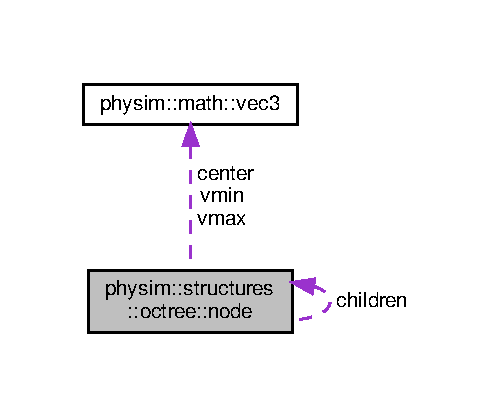
\includegraphics[width=236pt]{structphysim_1_1structures_1_1octree_1_1node__coll__graph}
\end{center}
\end{figure}
\subsection*{Public Member Functions}
\begin{DoxyCompactItemize}
\item 
\mbox{\Hypertarget{structphysim_1_1structures_1_1octree_1_1node_a635b012328b2533bb5ed7426a405629c}\label{structphysim_1_1structures_1_1octree_1_1node_a635b012328b2533bb5ed7426a405629c}} 
\hyperlink{structphysim_1_1structures_1_1octree_1_1node_a635b012328b2533bb5ed7426a405629c}{node} ()
\begin{DoxyCompactList}\small\item\em Default constructor. Initialises pointers to null. \end{DoxyCompactList}\item 
\mbox{\Hypertarget{structphysim_1_1structures_1_1octree_1_1node_a3a4c3b8ddc5369ddef78d72bc8f5782b}\label{structphysim_1_1structures_1_1octree_1_1node_a3a4c3b8ddc5369ddef78d72bc8f5782b}} 
\hyperlink{structphysim_1_1structures_1_1octree_1_1node_a3a4c3b8ddc5369ddef78d72bc8f5782b}{$\sim$node} ()
\begin{DoxyCompactList}\small\item\em Destructor. \end{DoxyCompactList}\item 
\mbox{\Hypertarget{structphysim_1_1structures_1_1octree_1_1node_a27550f838cc161e335d23c530257424b}\label{structphysim_1_1structures_1_1octree_1_1node_a27550f838cc161e335d23c530257424b}} 
size\+\_\+t $\ast$ \hyperlink{structphysim_1_1structures_1_1octree_1_1node_a27550f838cc161e335d23c530257424b}{begin\+\_\+idxs} ()
\begin{DoxyCompactList}\small\item\em Returns a pointer to the beginning of \hyperlink{structphysim_1_1structures_1_1octree_1_1node_ae365c35e35e5953164597fdb4264ab87}{idxs}. \end{DoxyCompactList}\item 
\mbox{\Hypertarget{structphysim_1_1structures_1_1octree_1_1node_adf9df754e0b826b53c09e0c5a2c8deab}\label{structphysim_1_1structures_1_1octree_1_1node_adf9df754e0b826b53c09e0c5a2c8deab}} 
const size\+\_\+t $\ast$ \hyperlink{structphysim_1_1structures_1_1octree_1_1node_adf9df754e0b826b53c09e0c5a2c8deab}{begin\+\_\+idxs} () const
\begin{DoxyCompactList}\small\item\em Returns a constant pointer to the beginning of \hyperlink{structphysim_1_1structures_1_1octree_1_1node_ae365c35e35e5953164597fdb4264ab87}{idxs}. \end{DoxyCompactList}\item 
\mbox{\Hypertarget{structphysim_1_1structures_1_1octree_1_1node_afe439da126264d23c11dc321324e6c70}\label{structphysim_1_1structures_1_1octree_1_1node_afe439da126264d23c11dc321324e6c70}} 
size\+\_\+t $\ast$ \hyperlink{structphysim_1_1structures_1_1octree_1_1node_afe439da126264d23c11dc321324e6c70}{end\+\_\+idxs} ()
\begin{DoxyCompactList}\small\item\em Returns a pointer to the ending of \hyperlink{structphysim_1_1structures_1_1octree_1_1node_ae365c35e35e5953164597fdb4264ab87}{idxs}. \end{DoxyCompactList}\item 
\mbox{\Hypertarget{structphysim_1_1structures_1_1octree_1_1node_a5c026947781722c2f5c78cb97f4e5fee}\label{structphysim_1_1structures_1_1octree_1_1node_a5c026947781722c2f5c78cb97f4e5fee}} 
const size\+\_\+t $\ast$ \hyperlink{structphysim_1_1structures_1_1octree_1_1node_a5c026947781722c2f5c78cb97f4e5fee}{end\+\_\+idxs} () const
\begin{DoxyCompactList}\small\item\em Returns a constant pointer to the ending of \hyperlink{structphysim_1_1structures_1_1octree_1_1node_ae365c35e35e5953164597fdb4264ab87}{idxs}. \end{DoxyCompactList}\end{DoxyCompactItemize}
\subsection*{Public Attributes}
\begin{DoxyCompactItemize}
\item 
\mbox{\Hypertarget{structphysim_1_1structures_1_1octree_1_1node_a613c0a9c31c695326c8e93960fef02c0}\label{structphysim_1_1structures_1_1octree_1_1node_a613c0a9c31c695326c8e93960fef02c0}} 
\hyperlink{structphysim_1_1math_1_1vec3}{math\+::vec3} \hyperlink{structphysim_1_1structures_1_1octree_1_1node_a613c0a9c31c695326c8e93960fef02c0}{vmin}
\begin{DoxyCompactList}\small\item\em Points with the minimum coordinate values of the points within. \end{DoxyCompactList}\item 
\mbox{\Hypertarget{structphysim_1_1structures_1_1octree_1_1node_a24c7a2173e6a9fe1b90af08515f442a6}\label{structphysim_1_1structures_1_1octree_1_1node_a24c7a2173e6a9fe1b90af08515f442a6}} 
\hyperlink{structphysim_1_1math_1_1vec3}{math\+::vec3} \hyperlink{structphysim_1_1structures_1_1octree_1_1node_a24c7a2173e6a9fe1b90af08515f442a6}{vmax}
\begin{DoxyCompactList}\small\item\em Points with the maximum coordinate values of the points within. \end{DoxyCompactList}\item 
\mbox{\Hypertarget{structphysim_1_1structures_1_1octree_1_1node_affc727be57e0ed71aba4fa7abc61825a}\label{structphysim_1_1structures_1_1octree_1_1node_affc727be57e0ed71aba4fa7abc61825a}} 
\hyperlink{structphysim_1_1math_1_1vec3}{math\+::vec3} \hyperlink{structphysim_1_1structures_1_1octree_1_1node_affc727be57e0ed71aba4fa7abc61825a}{center}
\begin{DoxyCompactList}\small\item\em Point at the center of the region this node partitions. \end{DoxyCompactList}\item 
\mbox{\Hypertarget{structphysim_1_1structures_1_1octree_1_1node_ae365c35e35e5953164597fdb4264ab87}\label{structphysim_1_1structures_1_1octree_1_1node_ae365c35e35e5953164597fdb4264ab87}} 
size\+\_\+t $\ast$ \hyperlink{structphysim_1_1structures_1_1octree_1_1node_ae365c35e35e5953164597fdb4264ab87}{idxs}
\begin{DoxyCompactList}\small\item\em Indices to the objects\textquotesingle{} indices. \end{DoxyCompactList}\item 
\mbox{\Hypertarget{structphysim_1_1structures_1_1octree_1_1node_ac8fab592afa663512b66c04a794d85a3}\label{structphysim_1_1structures_1_1octree_1_1node_ac8fab592afa663512b66c04a794d85a3}} 
size\+\_\+t \hyperlink{structphysim_1_1structures_1_1octree_1_1node_ac8fab592afa663512b66c04a794d85a3}{count}
\begin{DoxyCompactList}\small\item\em Amount of indices stored. \end{DoxyCompactList}\item 
\mbox{\Hypertarget{structphysim_1_1structures_1_1octree_1_1node_a171e9edaf00329bb27e4014b13eb5445}\label{structphysim_1_1structures_1_1octree_1_1node_a171e9edaf00329bb27e4014b13eb5445}} 
bool \hyperlink{structphysim_1_1structures_1_1octree_1_1node_a171e9edaf00329bb27e4014b13eb5445}{leaf}
\begin{DoxyCompactList}\small\item\em Is this node a leaf? \end{DoxyCompactList}\item 
\mbox{\Hypertarget{structphysim_1_1structures_1_1octree_1_1node_ad2a9bf9588293e39212fc909fc4bcd58}\label{structphysim_1_1structures_1_1octree_1_1node_ad2a9bf9588293e39212fc909fc4bcd58}} 
\hyperlink{structphysim_1_1structures_1_1octree_1_1node}{node} $\ast$ \hyperlink{structphysim_1_1structures_1_1octree_1_1node_ad2a9bf9588293e39212fc909fc4bcd58}{children} \mbox{[}8\mbox{]}
\begin{DoxyCompactList}\small\item\em Pointers to the children of this node. \end{DoxyCompactList}\end{DoxyCompactItemize}


\subsection{Detailed Description}
Octree\textquotesingle{}s node definition. 

The documentation for this struct was generated from the following files\+:\begin{DoxyCompactItemize}
\item 
physim/structures/octree.\+hpp\item 
physim/structures/octree.\+cpp\end{DoxyCompactItemize}

\hypertarget{classphysim_1_1geometric_1_1object}{}\section{physim\+:\+:geometric\+:\+:object Class Reference}
\label{classphysim_1_1geometric_1_1object}\index{physim\+::geometric\+::object@{physim\+::geometric\+::object}}


Class that implements a triangular object.  




{\ttfamily \#include $<$object.\+hpp$>$}



Inheritance diagram for physim\+:\+:geometric\+:\+:object\+:\nopagebreak
\begin{figure}[H]
\begin{center}
\leavevmode
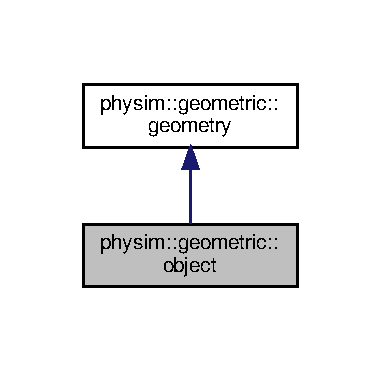
\includegraphics[width=183pt]{classphysim_1_1geometric_1_1object__inherit__graph}
\end{center}
\end{figure}


Collaboration diagram for physim\+:\+:geometric\+:\+:object\+:\nopagebreak
\begin{figure}[H]
\begin{center}
\leavevmode
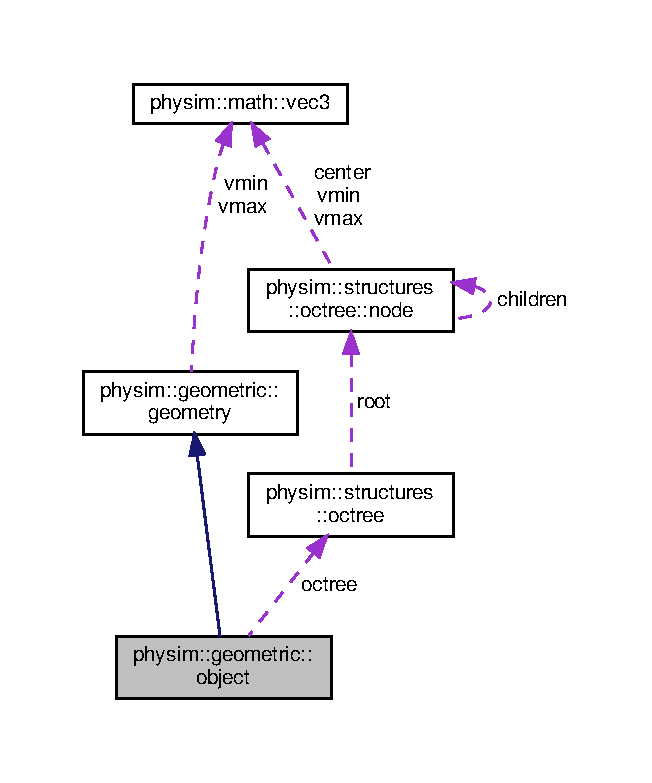
\includegraphics[width=313pt]{classphysim_1_1geometric_1_1object__coll__graph}
\end{center}
\end{figure}
\subsection*{Public Member Functions}
\begin{DoxyCompactItemize}
\item 
\mbox{\Hypertarget{classphysim_1_1geometric_1_1object_aa6db7d14fdf7c82dfdbd1f309aefa23b}\label{classphysim_1_1geometric_1_1object_aa6db7d14fdf7c82dfdbd1f309aefa23b}} 
\hyperlink{classphysim_1_1geometric_1_1object_aa6db7d14fdf7c82dfdbd1f309aefa23b}{object} ()
\begin{DoxyCompactList}\small\item\em Default constructor. \end{DoxyCompactList}\item 
\mbox{\Hypertarget{classphysim_1_1geometric_1_1object_a5fbc926d0a13708ec44d4dd06183d8c1}\label{classphysim_1_1geometric_1_1object_a5fbc926d0a13708ec44d4dd06183d8c1}} 
\hyperlink{classphysim_1_1geometric_1_1object_a5fbc926d0a13708ec44d4dd06183d8c1}{object} (const \hyperlink{classphysim_1_1geometric_1_1object}{object} \&p)
\begin{DoxyCompactList}\small\item\em Copy constructor. \end{DoxyCompactList}\item 
\mbox{\Hypertarget{classphysim_1_1geometric_1_1object_a1a013449e416aa0df0b9859fe6c31548}\label{classphysim_1_1geometric_1_1object_a1a013449e416aa0df0b9859fe6c31548}} 
\hyperlink{classphysim_1_1geometric_1_1object_a1a013449e416aa0df0b9859fe6c31548}{$\sim$object} ()
\begin{DoxyCompactList}\small\item\em Destructor. \end{DoxyCompactList}\item 
void \hyperlink{classphysim_1_1geometric_1_1object_ab1efcebf4013206cee817beeb0415cd6}{set\+\_\+position} (const \hyperlink{structphysim_1_1math_1_1vec3}{math\+::vec3} \&v)
\begin{DoxyCompactList}\small\item\em Sets the position of this object. \end{DoxyCompactList}\item 
void \hyperlink{classphysim_1_1geometric_1_1object_a637c4792d486f76fb0c0dabeb0b468ea}{set\+\_\+triangles} (const std\+::vector$<$ \hyperlink{structphysim_1_1math_1_1vec3}{math\+::vec3} $>$ \&vs, const std\+::vector$<$ size\+\_\+t $>$ \&trs)
\begin{DoxyCompactList}\small\item\em Constructs this object with triangles. \end{DoxyCompactList}\item 
const \hyperlink{classphysim_1_1structures_1_1octree}{structures\+::octree} \& \hyperlink{classphysim_1_1geometric_1_1object_a618389ab9b30e9dea436165a6920b389}{get\+\_\+partition} () const
\begin{DoxyCompactList}\small\item\em Returns the underlying structure that partitions this object. \end{DoxyCompactList}\item 
\mbox{\Hypertarget{classphysim_1_1geometric_1_1object_af631872682ea6a44bdebe5f9f9f98ab8}\label{classphysim_1_1geometric_1_1object_af631872682ea6a44bdebe5f9f9f98ab8}} 
\hyperlink{namespacephysim_1_1geometric_ac2794fff270c5b2ff4307f107a365fca}{geometry\+\_\+type} \hyperlink{classphysim_1_1geometric_1_1object_af631872682ea6a44bdebe5f9f9f98ab8}{get\+\_\+geom\+\_\+type} () const
\begin{DoxyCompactList}\small\item\em Returns the type of geometry of this object. \end{DoxyCompactList}\item 
const std\+::vector$<$ \hyperlink{classphysim_1_1geometric_1_1triangle}{triangle} $>$ \& \hyperlink{classphysim_1_1geometric_1_1object_a4bdf008b324fe8e1e1b83dbc47b5e897}{get\+\_\+triangles} () const
\begin{DoxyCompactList}\small\item\em Returns the triangles of this object. \end{DoxyCompactList}\item 
bool \hyperlink{classphysim_1_1geometric_1_1object_ade3bdbcb865c6b0910b8adfe2225be9b}{is\+\_\+inside} (const \hyperlink{structphysim_1_1math_1_1vec3}{math\+::vec3} \&p, float tol=1.e-\/6f) const
\begin{DoxyCompactList}\small\item\em Returns true if {\itshape p} is inside the object. \end{DoxyCompactList}\item 
bool \hyperlink{classphysim_1_1geometric_1_1object_a1bb905634af6176cc88680ce6f9fb080}{intersec\+\_\+segment} (const \hyperlink{structphysim_1_1math_1_1vec3}{math\+::vec3} \&p1, const \hyperlink{structphysim_1_1math_1_1vec3}{math\+::vec3} \&p2) const
\begin{DoxyCompactList}\small\item\em Returns if the segment defined by the points {\itshape p1} and {\itshape p2} intersects the geometry. \end{DoxyCompactList}\item 
bool \hyperlink{classphysim_1_1geometric_1_1object_a10ee0f5a42edf3c469a9354a11571aac}{intersec\+\_\+segment} (const \hyperlink{structphysim_1_1math_1_1vec3}{math\+::vec3} \&p1, const \hyperlink{structphysim_1_1math_1_1vec3}{math\+::vec3} \&p2, \hyperlink{structphysim_1_1math_1_1vec3}{math\+::vec3} \&p\+\_\+inter) const
\begin{DoxyCompactList}\small\item\em Returns true if the segment \mbox{[}{\itshape p1}, {\itshape p2} \mbox{]} intersects with the geometry. \end{DoxyCompactList}\item 
bool \hyperlink{classphysim_1_1geometric_1_1object_a2846f76ef5b800bc50b6fa7e0a478a80}{intersec\+\_\+sphere} (const \hyperlink{structphysim_1_1math_1_1vec3}{math\+::vec3} \&c, float R) const
\begin{DoxyCompactList}\small\item\em Returns if the sphere with center the point {\itshape c} and radius {\itshape R} intersects the geometry. \end{DoxyCompactList}\item 
void \hyperlink{classphysim_1_1geometric_1_1object_a9885341b8bad60413402d84249bea9a2}{update\+\_\+particle} (const \hyperlink{structphysim_1_1math_1_1vec3}{math\+::vec3} \&pp, const \hyperlink{structphysim_1_1math_1_1vec3}{math\+::vec3} \&pv, \hyperlink{classphysim_1_1particles_1_1free__particle}{particles\+::free\+\_\+particle} \&p) const
\begin{DoxyCompactList}\small\item\em Update a free particle in a collision with geometry. \end{DoxyCompactList}\item 
bool \hyperlink{classphysim_1_1geometric_1_1object_a1d9063dda2c637490c15fddc8f0281cf}{update\+\_\+particle} (const \hyperlink{structphysim_1_1math_1_1vec3}{math\+::vec3} \&pp, const \hyperlink{structphysim_1_1math_1_1vec3}{math\+::vec3} \&pv, const \hyperlink{classphysim_1_1particles_1_1free__particle}{particles\+::free\+\_\+particle} \&p, \hyperlink{classphysim_1_1particles_1_1free__particle}{particles\+::free\+\_\+particle} \&u) const
\begin{DoxyCompactList}\small\item\em Updates a particle when its trajectory intersects this object. \end{DoxyCompactList}\item 
void \hyperlink{classphysim_1_1geometric_1_1object_aa9f27d1cc4ee3a3b9883bd155435c2bc}{update\+\_\+particle} (const \hyperlink{structphysim_1_1math_1_1vec3}{math\+::vec3} \&pp, const \hyperlink{structphysim_1_1math_1_1vec3}{math\+::vec3} \&pv, \hyperlink{classphysim_1_1particles_1_1sized__particle}{particles\+::sized\+\_\+particle} \&p) const
\begin{DoxyCompactList}\small\item\em Update a sized particle in a collision with geometry. \end{DoxyCompactList}\item 
bool \hyperlink{classphysim_1_1geometric_1_1object_a781f069a0b1a3ebc740382db21ec629c}{update\+\_\+particle} (const \hyperlink{structphysim_1_1math_1_1vec3}{math\+::vec3} \&pp, const \hyperlink{structphysim_1_1math_1_1vec3}{math\+::vec3} \&pv, const \hyperlink{classphysim_1_1particles_1_1sized__particle}{particles\+::sized\+\_\+particle} \&p, \hyperlink{classphysim_1_1particles_1_1sized__particle}{particles\+::sized\+\_\+particle} \&u) const
\begin{DoxyCompactList}\small\item\em Updates a particle when its trajectory intersects this object. \end{DoxyCompactList}\item 
\mbox{\Hypertarget{classphysim_1_1geometric_1_1object_ae1124726aaf9819fda672674c69f6d6c}\label{classphysim_1_1geometric_1_1object_ae1124726aaf9819fda672674c69f6d6c}} 
void \hyperlink{classphysim_1_1geometric_1_1object_ae1124726aaf9819fda672674c69f6d6c}{display} () const
\begin{DoxyCompactList}\small\item\em Output on stream {\itshape cout} information about this geometry. \end{DoxyCompactList}\end{DoxyCompactItemize}
\subsection*{Private Attributes}
\begin{DoxyCompactItemize}
\item 
\mbox{\Hypertarget{classphysim_1_1geometric_1_1object_a0a7ba3bc4dda95651acdc046342e437c}\label{classphysim_1_1geometric_1_1object_a0a7ba3bc4dda95651acdc046342e437c}} 
std\+::vector$<$ \hyperlink{classphysim_1_1geometric_1_1triangle}{triangle} $>$ \hyperlink{classphysim_1_1geometric_1_1object_a0a7ba3bc4dda95651acdc046342e437c}{tris}
\begin{DoxyCompactList}\small\item\em The triangles of this object. \end{DoxyCompactList}\item 
\mbox{\Hypertarget{classphysim_1_1geometric_1_1object_a4f588a490ec8a223b5229c6e7dba5295}\label{classphysim_1_1geometric_1_1object_a4f588a490ec8a223b5229c6e7dba5295}} 
\hyperlink{classphysim_1_1structures_1_1octree}{structures\+::octree} \hyperlink{classphysim_1_1geometric_1_1object_a4f588a490ec8a223b5229c6e7dba5295}{octree}
\begin{DoxyCompactList}\small\item\em Partition of the object for faster intersection tests. \end{DoxyCompactList}\end{DoxyCompactItemize}
\subsection*{Additional Inherited Members}


\subsection{Detailed Description}
Class that implements a triangular object. 

A triangular object is a collection of triangles which may be a triangle soup or a triangular mesh. 

\subsection{Member Function Documentation}
\mbox{\Hypertarget{classphysim_1_1geometric_1_1object_a618389ab9b30e9dea436165a6920b389}\label{classphysim_1_1geometric_1_1object_a618389ab9b30e9dea436165a6920b389}} 
\index{physim\+::geometric\+::object@{physim\+::geometric\+::object}!get\+\_\+partition@{get\+\_\+partition}}
\index{get\+\_\+partition@{get\+\_\+partition}!physim\+::geometric\+::object@{physim\+::geometric\+::object}}
\subsubsection{\texorpdfstring{get\+\_\+partition()}{get\_partition()}}
{\footnotesize\ttfamily const \hyperlink{classphysim_1_1structures_1_1octree}{structures\+::octree} \& physim\+::geometric\+::object\+::get\+\_\+partition (\begin{DoxyParamCaption}{ }\end{DoxyParamCaption}) const}



Returns the underlying structure that partitions this object. 

\begin{DoxyReturn}{Returns}
Returns a constant reference to \hyperlink{classphysim_1_1geometric_1_1object_a4f588a490ec8a223b5229c6e7dba5295}{octree}. 
\end{DoxyReturn}
\mbox{\Hypertarget{classphysim_1_1geometric_1_1object_a4bdf008b324fe8e1e1b83dbc47b5e897}\label{classphysim_1_1geometric_1_1object_a4bdf008b324fe8e1e1b83dbc47b5e897}} 
\index{physim\+::geometric\+::object@{physim\+::geometric\+::object}!get\+\_\+triangles@{get\+\_\+triangles}}
\index{get\+\_\+triangles@{get\+\_\+triangles}!physim\+::geometric\+::object@{physim\+::geometric\+::object}}
\subsubsection{\texorpdfstring{get\+\_\+triangles()}{get\_triangles()}}
{\footnotesize\ttfamily const std\+::vector$<$ \hyperlink{classphysim_1_1geometric_1_1triangle}{triangle} $>$ \& physim\+::geometric\+::object\+::get\+\_\+triangles (\begin{DoxyParamCaption}{ }\end{DoxyParamCaption}) const}



Returns the triangles of this object. 

\begin{DoxyReturn}{Returns}
Returns a constant reference to \hyperlink{classphysim_1_1geometric_1_1object_a0a7ba3bc4dda95651acdc046342e437c}{tris}. 
\end{DoxyReturn}
\mbox{\Hypertarget{classphysim_1_1geometric_1_1object_a1bb905634af6176cc88680ce6f9fb080}\label{classphysim_1_1geometric_1_1object_a1bb905634af6176cc88680ce6f9fb080}} 
\index{physim\+::geometric\+::object@{physim\+::geometric\+::object}!intersec\+\_\+segment@{intersec\+\_\+segment}}
\index{intersec\+\_\+segment@{intersec\+\_\+segment}!physim\+::geometric\+::object@{physim\+::geometric\+::object}}
\subsubsection{\texorpdfstring{intersec\+\_\+segment()}{intersec\_segment()}\hspace{0.1cm}{\footnotesize\ttfamily [1/2]}}
{\footnotesize\ttfamily bool physim\+::geometric\+::object\+::intersec\+\_\+segment (\begin{DoxyParamCaption}\item[{const \hyperlink{structphysim_1_1math_1_1vec3}{math\+::vec3} \&}]{p1,  }\item[{const \hyperlink{structphysim_1_1math_1_1vec3}{math\+::vec3} \&}]{p2 }\end{DoxyParamCaption}) const\hspace{0.3cm}{\ttfamily [virtual]}}



Returns if the segment defined by the points {\itshape p1} and {\itshape p2} intersects the geometry. 


\begin{DoxyParams}[1]{Parameters}
\mbox{\tt in}  & {\em p1} & First endpoint of the segment. \\
\hline
\mbox{\tt in}  & {\em p2} & Second endpoint of the segment. \\
\hline
\end{DoxyParams}
\begin{DoxyReturn}{Returns}
Returns true if there is intersection. 
\end{DoxyReturn}


Implements \hyperlink{classphysim_1_1geometric_1_1geometry_a63d63c340937cede50a95903679c5ad3}{physim\+::geometric\+::geometry}.

\mbox{\Hypertarget{classphysim_1_1geometric_1_1object_a10ee0f5a42edf3c469a9354a11571aac}\label{classphysim_1_1geometric_1_1object_a10ee0f5a42edf3c469a9354a11571aac}} 
\index{physim\+::geometric\+::object@{physim\+::geometric\+::object}!intersec\+\_\+segment@{intersec\+\_\+segment}}
\index{intersec\+\_\+segment@{intersec\+\_\+segment}!physim\+::geometric\+::object@{physim\+::geometric\+::object}}
\subsubsection{\texorpdfstring{intersec\+\_\+segment()}{intersec\_segment()}\hspace{0.1cm}{\footnotesize\ttfamily [2/2]}}
{\footnotesize\ttfamily bool physim\+::geometric\+::object\+::intersec\+\_\+segment (\begin{DoxyParamCaption}\item[{const \hyperlink{structphysim_1_1math_1_1vec3}{math\+::vec3} \&}]{p1,  }\item[{const \hyperlink{structphysim_1_1math_1_1vec3}{math\+::vec3} \&}]{p2,  }\item[{\hyperlink{structphysim_1_1math_1_1vec3}{math\+::vec3} \&}]{p\+\_\+inter }\end{DoxyParamCaption}) const\hspace{0.3cm}{\ttfamily [virtual]}}



Returns true if the segment \mbox{[}{\itshape p1}, {\itshape p2} \mbox{]} intersects with the geometry. 


\begin{DoxyParams}[1]{Parameters}
\mbox{\tt in}  & {\em p1} & The first endpoint of the segment. \\
\hline
\mbox{\tt in}  & {\em p2} & The second endpoint of the segment. \\
\hline
\mbox{\tt out}  & {\em p\+\_\+inter} & The intersection point between the segment and the geometry. \\
\hline
\end{DoxyParams}
\begin{DoxyReturn}{Returns}
Returns true if the segment and the geometry intersect. In this case, the value in {\itshape p\+\_\+inter} will be the intersection point. 
\end{DoxyReturn}


Implements \hyperlink{classphysim_1_1geometric_1_1geometry_ae9fa877e89b7b2693a94d0772561ad9a}{physim\+::geometric\+::geometry}.

\mbox{\Hypertarget{classphysim_1_1geometric_1_1object_a2846f76ef5b800bc50b6fa7e0a478a80}\label{classphysim_1_1geometric_1_1object_a2846f76ef5b800bc50b6fa7e0a478a80}} 
\index{physim\+::geometric\+::object@{physim\+::geometric\+::object}!intersec\+\_\+sphere@{intersec\+\_\+sphere}}
\index{intersec\+\_\+sphere@{intersec\+\_\+sphere}!physim\+::geometric\+::object@{physim\+::geometric\+::object}}
\subsubsection{\texorpdfstring{intersec\+\_\+sphere()}{intersec\_sphere()}}
{\footnotesize\ttfamily bool physim\+::geometric\+::object\+::intersec\+\_\+sphere (\begin{DoxyParamCaption}\item[{const \hyperlink{structphysim_1_1math_1_1vec3}{math\+::vec3} \&}]{c,  }\item[{float}]{R }\end{DoxyParamCaption}) const\hspace{0.3cm}{\ttfamily [virtual]}}



Returns if the sphere with center the point {\itshape c} and radius {\itshape R} intersects the geometry. 


\begin{DoxyParams}[1]{Parameters}
\mbox{\tt in}  & {\em c} & Center of the sphere. \\
\hline
\mbox{\tt in}  & {\em R} & radius of the sphere. \\
\hline
\end{DoxyParams}
\begin{DoxyReturn}{Returns}
Returns true if there is intersection. 
\end{DoxyReturn}


Implements \hyperlink{classphysim_1_1geometric_1_1geometry_aab49e452a72d1ecaf434be2b8de98169}{physim\+::geometric\+::geometry}.

\mbox{\Hypertarget{classphysim_1_1geometric_1_1object_ade3bdbcb865c6b0910b8adfe2225be9b}\label{classphysim_1_1geometric_1_1object_ade3bdbcb865c6b0910b8adfe2225be9b}} 
\index{physim\+::geometric\+::object@{physim\+::geometric\+::object}!is\+\_\+inside@{is\+\_\+inside}}
\index{is\+\_\+inside@{is\+\_\+inside}!physim\+::geometric\+::object@{physim\+::geometric\+::object}}
\subsubsection{\texorpdfstring{is\+\_\+inside()}{is\_inside()}}
{\footnotesize\ttfamily bool physim\+::geometric\+::object\+::is\+\_\+inside (\begin{DoxyParamCaption}\item[{const \hyperlink{structphysim_1_1math_1_1vec3}{math\+::vec3} \&}]{p,  }\item[{float}]{tol = {\ttfamily 1.e-\/6f} }\end{DoxyParamCaption}) const\hspace{0.3cm}{\ttfamily [virtual]}}



Returns true if {\itshape p} is inside the object. 

Returns true iff {\itshape p} is inside any of triangles. See \hyperlink{classphysim_1_1geometric_1_1triangle_a735cfae7db71f5d6105011c40595ca37}{triangle\+::is\+\_\+inside}. 

Implements \hyperlink{classphysim_1_1geometric_1_1geometry_a325d4049d4e14584b389a2f1202bdc08}{physim\+::geometric\+::geometry}.

\mbox{\Hypertarget{classphysim_1_1geometric_1_1object_ab1efcebf4013206cee817beeb0415cd6}\label{classphysim_1_1geometric_1_1object_ab1efcebf4013206cee817beeb0415cd6}} 
\index{physim\+::geometric\+::object@{physim\+::geometric\+::object}!set\+\_\+position@{set\+\_\+position}}
\index{set\+\_\+position@{set\+\_\+position}!physim\+::geometric\+::object@{physim\+::geometric\+::object}}
\subsubsection{\texorpdfstring{set\+\_\+position()}{set\_position()}}
{\footnotesize\ttfamily void physim\+::geometric\+::object\+::set\+\_\+position (\begin{DoxyParamCaption}\item[{const \hyperlink{structphysim_1_1math_1_1vec3}{math\+::vec3} \&}]{v }\end{DoxyParamCaption})\hspace{0.3cm}{\ttfamily [virtual]}}



Sets the position of this object. 

Translates all triangles in \hyperlink{classphysim_1_1geometric_1_1object_a0a7ba3bc4dda95651acdc046342e437c}{tris} in the direction of vector {\itshape v}. 
\begin{DoxyParams}{Parameters}
{\em v} & Vector. \\
\hline
\end{DoxyParams}


Implements \hyperlink{classphysim_1_1geometric_1_1geometry_a5b029b5fa8e55847d5aa06b1d341c88c}{physim\+::geometric\+::geometry}.

\mbox{\Hypertarget{classphysim_1_1geometric_1_1object_a637c4792d486f76fb0c0dabeb0b468ea}\label{classphysim_1_1geometric_1_1object_a637c4792d486f76fb0c0dabeb0b468ea}} 
\index{physim\+::geometric\+::object@{physim\+::geometric\+::object}!set\+\_\+triangles@{set\+\_\+triangles}}
\index{set\+\_\+triangles@{set\+\_\+triangles}!physim\+::geometric\+::object@{physim\+::geometric\+::object}}
\subsubsection{\texorpdfstring{set\+\_\+triangles()}{set\_triangles()}}
{\footnotesize\ttfamily void physim\+::geometric\+::object\+::set\+\_\+triangles (\begin{DoxyParamCaption}\item[{const std\+::vector$<$ \hyperlink{structphysim_1_1math_1_1vec3}{math\+::vec3} $>$ \&}]{vs,  }\item[{const std\+::vector$<$ size\+\_\+t $>$ \&}]{trs }\end{DoxyParamCaption})}



Constructs this object with triangles. 

Sets the triangles of this object (see \hyperlink{classphysim_1_1geometric_1_1object_a0a7ba3bc4dda95651acdc046342e437c}{tris}), and constructs its partition (see \hyperlink{classphysim_1_1geometric_1_1object_a4f588a490ec8a223b5229c6e7dba5295}{octree}). 
\begin{DoxyParams}{Parameters}
{\em vs} & Vertices of the object. \\
\hline
{\em trs} & Triangles of the object. This contains indices pointing to vertices in {\itshape vs}. Every three values we have a triangle. \\
\hline
\end{DoxyParams}
\mbox{\Hypertarget{classphysim_1_1geometric_1_1object_a9885341b8bad60413402d84249bea9a2}\label{classphysim_1_1geometric_1_1object_a9885341b8bad60413402d84249bea9a2}} 
\index{physim\+::geometric\+::object@{physim\+::geometric\+::object}!update\+\_\+particle@{update\+\_\+particle}}
\index{update\+\_\+particle@{update\+\_\+particle}!physim\+::geometric\+::object@{physim\+::geometric\+::object}}
\subsubsection{\texorpdfstring{update\+\_\+particle()}{update\_particle()}\hspace{0.1cm}{\footnotesize\ttfamily [1/4]}}
{\footnotesize\ttfamily void physim\+::geometric\+::object\+::update\+\_\+particle (\begin{DoxyParamCaption}\item[{const \hyperlink{structphysim_1_1math_1_1vec3}{math\+::vec3} \&}]{pred\+\_\+pos,  }\item[{const \hyperlink{structphysim_1_1math_1_1vec3}{math\+::vec3} \&}]{pred\+\_\+vel,  }\item[{\hyperlink{classphysim_1_1particles_1_1free__particle}{particles\+::free\+\_\+particle} \&}]{pred }\end{DoxyParamCaption}) const\hspace{0.3cm}{\ttfamily [virtual]}}



Update a free particle in a collision with geometry. 

Assumig that particle {\itshape pred} collided with this geometry, update its position, velocity, ... accordingly.

For example, some geometry may be \textquotesingle{}bouncy\textquotesingle{}, it may give the particle some extra speed. This needs to be updated in this method.

The particle {\itshape pred} is given in a state that is not modified by any solver. That is, the particle\textquotesingle{}s position, velocity, force, ... have the value at time step {\itshape T}. The predicted position and velocity are given in {\itshape pred\+\_\+pos} and {\itshape pred\+\_\+vel}. These are predictions of the position and velocity for time {\itshape T} + {\itshape dt} (where dt is some time step). The modified particle due to the collision must be stored in {\itshape pred}.

This method is called only when it is sure that there has been a collision\+: the segment joining the particle\textquotesingle{}s current position and the predicted position intersects the geometry.


\begin{DoxyParams}[1]{Parameters}
\mbox{\tt in}  & {\em pred\+\_\+pos} & The predicted position of the particle. \\
\hline
\mbox{\tt in}  & {\em pred\+\_\+vel} & The predicted velocity of the particle. \\
\hline
\mbox{\tt out}  & {\em pred} & The particle with the result of the collision. \\
\hline
\end{DoxyParams}


Implements \hyperlink{classphysim_1_1geometric_1_1geometry_ae5d606ba51451b964fcb2301d5622cab}{physim\+::geometric\+::geometry}.

\mbox{\Hypertarget{classphysim_1_1geometric_1_1object_a1d9063dda2c637490c15fddc8f0281cf}\label{classphysim_1_1geometric_1_1object_a1d9063dda2c637490c15fddc8f0281cf}} 
\index{physim\+::geometric\+::object@{physim\+::geometric\+::object}!update\+\_\+particle@{update\+\_\+particle}}
\index{update\+\_\+particle@{update\+\_\+particle}!physim\+::geometric\+::object@{physim\+::geometric\+::object}}
\subsubsection{\texorpdfstring{update\+\_\+particle()}{update\_particle()}\hspace{0.1cm}{\footnotesize\ttfamily [2/4]}}
{\footnotesize\ttfamily bool physim\+::geometric\+::object\+::update\+\_\+particle (\begin{DoxyParamCaption}\item[{const \hyperlink{structphysim_1_1math_1_1vec3}{math\+::vec3} \&}]{pp,  }\item[{const \hyperlink{structphysim_1_1math_1_1vec3}{math\+::vec3} \&}]{pv,  }\item[{const \hyperlink{classphysim_1_1particles_1_1free__particle}{particles\+::free\+\_\+particle} \&}]{p,  }\item[{\hyperlink{classphysim_1_1particles_1_1free__particle}{particles\+::free\+\_\+particle} \&}]{u }\end{DoxyParamCaption}) const}



Updates a particle when its trajectory intersects this object. 

See \hyperlink{classphysim_1_1geometric_1_1object_a9885341b8bad60413402d84249bea9a2}{update\+\_\+particle(const math\+::vec3\&, const math\+::vec3\&, particles\+::free\+\_\+particle\&)const} for details.

Prior to updating the position of {\itshape p}, its contents are copied into {\itshape u}.


\begin{DoxyParams}[1]{Parameters}
\mbox{\tt in}  & {\em pp} & The predicted position of the particle. \\
\hline
\mbox{\tt in}  & {\em pv} & The predicted velocity of the particle. \\
\hline
\mbox{\tt in}  & {\em p} & Original particle. This particle\textquotesingle{}s current position is used to construct the segment used in the intersection tests. \\
\hline
\mbox{\tt out}  & {\em u} & The particle with the result of the collision. \\
\hline
\end{DoxyParams}
\begin{DoxyReturn}{Returns}
Returns true if there was collision and the particle {\itshape u} was updated. 
\end{DoxyReturn}
\mbox{\Hypertarget{classphysim_1_1geometric_1_1object_aa9f27d1cc4ee3a3b9883bd155435c2bc}\label{classphysim_1_1geometric_1_1object_aa9f27d1cc4ee3a3b9883bd155435c2bc}} 
\index{physim\+::geometric\+::object@{physim\+::geometric\+::object}!update\+\_\+particle@{update\+\_\+particle}}
\index{update\+\_\+particle@{update\+\_\+particle}!physim\+::geometric\+::object@{physim\+::geometric\+::object}}
\subsubsection{\texorpdfstring{update\+\_\+particle()}{update\_particle()}\hspace{0.1cm}{\footnotesize\ttfamily [3/4]}}
{\footnotesize\ttfamily void physim\+::geometric\+::object\+::update\+\_\+particle (\begin{DoxyParamCaption}\item[{const \hyperlink{structphysim_1_1math_1_1vec3}{math\+::vec3} \&}]{pred\+\_\+pos,  }\item[{const \hyperlink{structphysim_1_1math_1_1vec3}{math\+::vec3} \&}]{pred\+\_\+vel,  }\item[{\hyperlink{classphysim_1_1particles_1_1sized__particle}{particles\+::sized\+\_\+particle} \&}]{pred }\end{DoxyParamCaption}) const\hspace{0.3cm}{\ttfamily [virtual]}}



Update a sized particle in a collision with geometry. 

Assumig that particle {\itshape pred} collided with this geometry, update its position, velocity, ... accordingly.

For example, some geometry may be \textquotesingle{}bouncy\textquotesingle{}, it may give the particle some extra speed. This needs to be updated in this method.

The particle {\itshape pred} is given in a state that is not modified by any solver. That is, the particle\textquotesingle{}s position, velocity, force, ... have the value at time step {\itshape T}. The predicted position and velocity are given in {\itshape pred\+\_\+pos} and {\itshape pred\+\_\+vel}. These are predictions of the position and velocity for time {\itshape T} + {\itshape dt} (where dt is some time step). The modified particle due to the collision must be stored in {\itshape pred}.

This method is called only when it is sure that there has been a collision\+: the segment joining the particle\textquotesingle{}s current position and the predicted position intersects the geometry.


\begin{DoxyParams}[1]{Parameters}
\mbox{\tt in}  & {\em pred\+\_\+pos} & The predicted position of the particle. \\
\hline
\mbox{\tt in}  & {\em pred\+\_\+vel} & The predicted velocity of the particle. \\
\hline
\mbox{\tt out}  & {\em pred} & The particle with the result of the collision. \\
\hline
\end{DoxyParams}


Implements \hyperlink{classphysim_1_1geometric_1_1geometry_a11c26d2fea85bf7bc41ec94cefa9729e}{physim\+::geometric\+::geometry}.

\mbox{\Hypertarget{classphysim_1_1geometric_1_1object_a781f069a0b1a3ebc740382db21ec629c}\label{classphysim_1_1geometric_1_1object_a781f069a0b1a3ebc740382db21ec629c}} 
\index{physim\+::geometric\+::object@{physim\+::geometric\+::object}!update\+\_\+particle@{update\+\_\+particle}}
\index{update\+\_\+particle@{update\+\_\+particle}!physim\+::geometric\+::object@{physim\+::geometric\+::object}}
\subsubsection{\texorpdfstring{update\+\_\+particle()}{update\_particle()}\hspace{0.1cm}{\footnotesize\ttfamily [4/4]}}
{\footnotesize\ttfamily bool physim\+::geometric\+::object\+::update\+\_\+particle (\begin{DoxyParamCaption}\item[{const \hyperlink{structphysim_1_1math_1_1vec3}{math\+::vec3} \&}]{pp,  }\item[{const \hyperlink{structphysim_1_1math_1_1vec3}{math\+::vec3} \&}]{pv,  }\item[{const \hyperlink{classphysim_1_1particles_1_1sized__particle}{particles\+::sized\+\_\+particle} \&}]{p,  }\item[{\hyperlink{classphysim_1_1particles_1_1sized__particle}{particles\+::sized\+\_\+particle} \&}]{u }\end{DoxyParamCaption}) const}



Updates a particle when its trajectory intersects this object. 

See \hyperlink{classphysim_1_1geometric_1_1object_aa9f27d1cc4ee3a3b9883bd155435c2bc}{update\+\_\+particle(const math\+::vec3\&, const math\+::vec3\&, particles\+::sized\+\_\+particle\&)const} for details.

Prior to updating the position of {\itshape p}, its contents are copied into {\itshape u}.


\begin{DoxyParams}[1]{Parameters}
\mbox{\tt in}  & {\em pp} & The predicted position of the particle. \\
\hline
\mbox{\tt in}  & {\em pv} & The predicted velocity of the particle. \\
\hline
\mbox{\tt in}  & {\em p} & Original particle. This particle\textquotesingle{}s current position is used to construct the segment used in the intersection tests. \\
\hline
\mbox{\tt out}  & {\em u} & The particle with the result of the collision. \\
\hline
\end{DoxyParams}
\begin{DoxyReturn}{Returns}
Returns true if there was collision and the particle {\itshape u} was updated. 
\end{DoxyReturn}


The documentation for this class was generated from the following files\+:\begin{DoxyCompactItemize}
\item 
physim/geometry/object.\+hpp\item 
physim/geometry/object.\+cpp\end{DoxyCompactItemize}

\hypertarget{classphysim_1_1structures_1_1octree}{}\section{physim\+:\+:structures\+:\+:octree Class Reference}
\label{classphysim_1_1structures_1_1octree}\index{physim\+::structures\+::octree@{physim\+::structures\+::octree}}


Octree class.  




{\ttfamily \#include $<$octree.\+hpp$>$}



Collaboration diagram for physim\+:\+:structures\+:\+:octree\+:\nopagebreak
\begin{figure}[H]
\begin{center}
\leavevmode
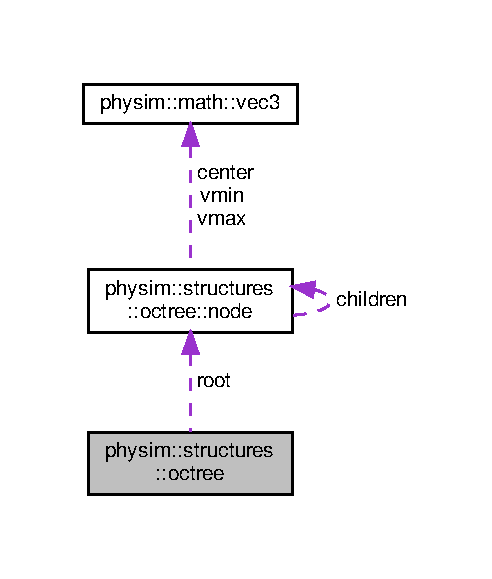
\includegraphics[width=236pt]{classphysim_1_1structures_1_1octree__coll__graph}
\end{center}
\end{figure}
\subsection*{Classes}
\begin{DoxyCompactItemize}
\item 
struct \hyperlink{structphysim_1_1structures_1_1octree_1_1node}{node}
\begin{DoxyCompactList}\small\item\em Octree\textquotesingle{}s node definition. \end{DoxyCompactList}\end{DoxyCompactItemize}
\subsection*{Public Member Functions}
\begin{DoxyCompactItemize}
\item 
\mbox{\Hypertarget{classphysim_1_1structures_1_1octree_ae8f02259c6494f8529542ae3bbd8e89f}\label{classphysim_1_1structures_1_1octree_ae8f02259c6494f8529542ae3bbd8e89f}} 
\hyperlink{classphysim_1_1structures_1_1octree_ae8f02259c6494f8529542ae3bbd8e89f}{octree} ()
\begin{DoxyCompactList}\small\item\em Default constructor. \end{DoxyCompactList}\item 
\mbox{\Hypertarget{classphysim_1_1structures_1_1octree_a827e35f372995bf2906ab42da5d67a78}\label{classphysim_1_1structures_1_1octree_a827e35f372995bf2906ab42da5d67a78}} 
\hyperlink{classphysim_1_1structures_1_1octree_a827e35f372995bf2906ab42da5d67a78}{$\sim$octree} ()
\begin{DoxyCompactList}\small\item\em Destructor. \end{DoxyCompactList}\item 
void \hyperlink{classphysim_1_1structures_1_1octree_add00dd5e93158b3fb54a7c8e37f01e8f}{init} (const std\+::vector$<$ \hyperlink{structphysim_1_1math_1_1vec3}{math\+::vec3} $>$ \&vertices, const std\+::vector$<$ size\+\_\+t $>$ \&tris\+\_\+indices, size\+\_\+t lod=8)
\begin{DoxyCompactList}\small\item\em Builds the partition of an object. \end{DoxyCompactList}\item 
void \hyperlink{classphysim_1_1structures_1_1octree_a6b6f4eb568f298f92f2c25025c60a2e2}{init} (const std\+::vector$<$ \hyperlink{structphysim_1_1math_1_1vec3}{math\+::vec3} $>$ \&vertices, size\+\_\+t lod=8)
\begin{DoxyCompactList}\small\item\em Builds the partition of a cloud of points. \end{DoxyCompactList}\item 
void \hyperlink{classphysim_1_1structures_1_1octree_a193143baa82a028ca9f7c65d69b48246}{init} (const void $\ast$p, size\+\_\+t n, size\+\_\+t offset, size\+\_\+t lod=8)
\begin{DoxyCompactList}\small\item\em Builds the partition of a cloud of points. \end{DoxyCompactList}\item 
\mbox{\Hypertarget{classphysim_1_1structures_1_1octree_a67b90846b173c0f34606d0f718d44497}\label{classphysim_1_1structures_1_1octree_a67b90846b173c0f34606d0f718d44497}} 
void \hyperlink{classphysim_1_1structures_1_1octree_a67b90846b173c0f34606d0f718d44497}{clear} ()
\begin{DoxyCompactList}\small\item\em Frees the memory occupied by this object. \end{DoxyCompactList}\item 
void \hyperlink{classphysim_1_1structures_1_1octree_aefdcd3e41277fa5d639dc9452361cba5}{copy} (const \hyperlink{classphysim_1_1structures_1_1octree}{octree} \&part)
\begin{DoxyCompactList}\small\item\em Copies the partition passed as parameter. \end{DoxyCompactList}\item 
void \hyperlink{classphysim_1_1structures_1_1octree_a5416f8bedbc67dbb4b0d7614c7ef811a}{get\+\_\+indices} (const \hyperlink{structphysim_1_1math_1_1vec3}{math\+::vec3} \&p, std\+::vector$<$ size\+\_\+t $>$ \&idxs) const
\begin{DoxyCompactList}\small\item\em Retrieves the indices of the objects incident to the cell of a point. \end{DoxyCompactList}\item 
void \hyperlink{classphysim_1_1structures_1_1octree_a808087da71c7499ca78613f770b0083e}{get\+\_\+indices} (const \hyperlink{structphysim_1_1math_1_1vec3}{math\+::vec3} \&p, float R, std\+::vector$<$ size\+\_\+t $>$ \&idxs) const
\begin{DoxyCompactList}\small\item\em Retrieves the indices of the objects incident to the cells intersecting a sphere. \end{DoxyCompactList}\item 
void \hyperlink{classphysim_1_1structures_1_1octree_ab113e2fd11a5c146a4c35c6f3e8db63c}{get\+\_\+boxes} (std\+::vector$<$ std\+::pair$<$ \hyperlink{structphysim_1_1math_1_1vec3}{math\+::vec3}, \hyperlink{structphysim_1_1math_1_1vec3}{math\+::vec3} $>$ $>$ \&boxes) const
\begin{DoxyCompactList}\small\item\em Returns the bounding boxes of the cells in this octree. \end{DoxyCompactList}\end{DoxyCompactItemize}
\subsection*{Private Member Functions}
\begin{DoxyCompactItemize}
\item 
\hyperlink{structphysim_1_1structures_1_1octree_1_1node}{node} $\ast$ \hyperlink{classphysim_1_1structures_1_1octree_a7891cdfc782b4a6026167d692783306e}{make\+\_\+octree\+\_\+triangles} (size\+\_\+t lod, const \hyperlink{structphysim_1_1math_1_1vec3}{math\+::vec3} \&vmin, const \hyperlink{structphysim_1_1math_1_1vec3}{math\+::vec3} \&vmax, const std\+::vector$<$ \hyperlink{structphysim_1_1math_1_1vec3}{math\+::vec3} $>$ \&vertices, const std\+::vector$<$ size\+\_\+t $>$ \&triangles, const std\+::vector$<$ std\+::vector$<$ size\+\_\+t $>$ $>$ \&tris\+\_\+per\+\_\+vertex, const std\+::vector$<$ size\+\_\+t $>$ \&vertices\+\_\+idxs, const std\+::vector$<$ size\+\_\+t $>$ \&triangle\+\_\+idxs) const
\begin{DoxyCompactList}\small\item\em Builds a tree rooted at a node that partitions the triangles stored in {\itshape triangles} pointed by {\itshape triangle\+\_\+idxs}. \end{DoxyCompactList}\item 
\hyperlink{structphysim_1_1structures_1_1octree_1_1node}{node} $\ast$ \hyperlink{classphysim_1_1structures_1_1octree_a47755b22ab1c4231a1c2bcf7b5ef2fe9}{make\+\_\+octree\+\_\+vertices} (const void $\ast$it, size\+\_\+t offset, const \hyperlink{structphysim_1_1math_1_1vec3}{math\+::vec3} \&vmin, const \hyperlink{structphysim_1_1math_1_1vec3}{math\+::vec3} \&vmax, const std\+::vector$<$ size\+\_\+t $>$ \&vertices\+\_\+idxs, size\+\_\+t lod) const
\begin{DoxyCompactList}\small\item\em Builds a tree rooted at a node that partitions the vertices stored in {\itshape vertices} pointed by {\itshape vertices\+\_\+idxs}. \end{DoxyCompactList}\item 
\hyperlink{structphysim_1_1structures_1_1octree_1_1node}{node} $\ast$ \hyperlink{classphysim_1_1structures_1_1octree_a2c4f254c7dfac0ed6f0ee4197e1bdeac}{copy\+\_\+node} (const \hyperlink{structphysim_1_1structures_1_1octree_1_1node}{node} $\ast$n) const
\begin{DoxyCompactList}\small\item\em Copies a node. \end{DoxyCompactList}\item 
void \hyperlink{classphysim_1_1structures_1_1octree_a4cd66ca4218ba9ff09ba953c4264f8ed}{get\+\_\+boxes\+\_\+node} (const \hyperlink{structphysim_1_1structures_1_1octree_1_1node}{node} $\ast$n, std\+::vector$<$ std\+::pair$<$ \hyperlink{structphysim_1_1math_1_1vec3}{math\+::vec3}, \hyperlink{structphysim_1_1math_1_1vec3}{math\+::vec3} $>$ $>$ \&boxes) const
\begin{DoxyCompactList}\small\item\em Returns the bounding boxes of the cells in this octree. \end{DoxyCompactList}\item 
void \hyperlink{classphysim_1_1structures_1_1octree_aec88b11968f8899022a93cb22b900398}{get\+\_\+indices\+\_\+node} (const \hyperlink{structphysim_1_1math_1_1vec3}{math\+::vec3} \&p, float R, const \hyperlink{structphysim_1_1structures_1_1octree_1_1node}{node} $\ast$n, std\+::vector$<$ size\+\_\+t $>$ \&idxs) const
\begin{DoxyCompactList}\small\item\em Retrieves the indices stored at those cells intersecting a sphere of radius {\itshape R} centered at {\itshape p}. \end{DoxyCompactList}\end{DoxyCompactItemize}
\subsection*{Private Attributes}
\begin{DoxyCompactItemize}
\item 
\mbox{\Hypertarget{classphysim_1_1structures_1_1octree_a20e74f30f2e76fa03899e236fcedaac4}\label{classphysim_1_1structures_1_1octree_a20e74f30f2e76fa03899e236fcedaac4}} 
\hyperlink{structphysim_1_1structures_1_1octree_1_1node}{node} $\ast$ \hyperlink{classphysim_1_1structures_1_1octree_a20e74f30f2e76fa03899e236fcedaac4}{root}
\begin{DoxyCompactList}\small\item\em Root of the octree. \end{DoxyCompactList}\end{DoxyCompactItemize}


\subsection{Detailed Description}
Octree class. 

This is an implementation of a basic octree for both set of triangles (see function \hyperlink{classphysim_1_1structures_1_1octree_add00dd5e93158b3fb54a7c8e37f01e8f}{init(const std\+::vector$<$math\+::vec3$>$\&, const std\+::vector$<$size\+\_\+t$>$\&, size\+\_\+t)} ),

and a set of vertices (see function \hyperlink{classphysim_1_1structures_1_1octree_a6b6f4eb568f298f92f2c25025c60a2e2}{init(const std\+::vector$<$math\+::vec3$>$\&, size\+\_\+t)} ). 

\subsection{Member Function Documentation}
\mbox{\Hypertarget{classphysim_1_1structures_1_1octree_aefdcd3e41277fa5d639dc9452361cba5}\label{classphysim_1_1structures_1_1octree_aefdcd3e41277fa5d639dc9452361cba5}} 
\index{physim\+::structures\+::octree@{physim\+::structures\+::octree}!copy@{copy}}
\index{copy@{copy}!physim\+::structures\+::octree@{physim\+::structures\+::octree}}
\subsubsection{\texorpdfstring{copy()}{copy()}}
{\footnotesize\ttfamily void physim\+::structures\+::octree\+::copy (\begin{DoxyParamCaption}\item[{const \hyperlink{classphysim_1_1structures_1_1octree}{octree} \&}]{part }\end{DoxyParamCaption})}



Copies the partition passed as parameter. 

The contents of this partition are cleared. 
\begin{DoxyParams}{Parameters}
{\em part} & An object partition. \\
\hline
\end{DoxyParams}
\mbox{\Hypertarget{classphysim_1_1structures_1_1octree_a2c4f254c7dfac0ed6f0ee4197e1bdeac}\label{classphysim_1_1structures_1_1octree_a2c4f254c7dfac0ed6f0ee4197e1bdeac}} 
\index{physim\+::structures\+::octree@{physim\+::structures\+::octree}!copy\+\_\+node@{copy\+\_\+node}}
\index{copy\+\_\+node@{copy\+\_\+node}!physim\+::structures\+::octree@{physim\+::structures\+::octree}}
\subsubsection{\texorpdfstring{copy\+\_\+node()}{copy\_node()}}
{\footnotesize\ttfamily \hyperlink{structphysim_1_1structures_1_1octree_1_1node}{octree\+::node} $\ast$ physim\+::structures\+::octree\+::copy\+\_\+node (\begin{DoxyParamCaption}\item[{const \hyperlink{structphysim_1_1structures_1_1octree_1_1node}{node} $\ast$}]{n }\end{DoxyParamCaption}) const\hspace{0.3cm}{\ttfamily [private]}}



Copies a node. 

Recursively copies a node {\itshape n}. 
\begin{DoxyParams}{Parameters}
{\em n} & Node to be copied. \\
\hline
\end{DoxyParams}
\begin{DoxyReturn}{Returns}
Reference to a node created in this function, a copy of {\itshape n}. 
\end{DoxyReturn}
\mbox{\Hypertarget{classphysim_1_1structures_1_1octree_ab113e2fd11a5c146a4c35c6f3e8db63c}\label{classphysim_1_1structures_1_1octree_ab113e2fd11a5c146a4c35c6f3e8db63c}} 
\index{physim\+::structures\+::octree@{physim\+::structures\+::octree}!get\+\_\+boxes@{get\+\_\+boxes}}
\index{get\+\_\+boxes@{get\+\_\+boxes}!physim\+::structures\+::octree@{physim\+::structures\+::octree}}
\subsubsection{\texorpdfstring{get\+\_\+boxes()}{get\_boxes()}}
{\footnotesize\ttfamily void physim\+::structures\+::octree\+::get\+\_\+boxes (\begin{DoxyParamCaption}\item[{std\+::vector$<$ std\+::pair$<$ \hyperlink{structphysim_1_1math_1_1vec3}{math\+::vec3}, \hyperlink{structphysim_1_1math_1_1vec3}{math\+::vec3} $>$ $>$ \&}]{boxes }\end{DoxyParamCaption}) const}



Returns the bounding boxes of the cells in this octree. 


\begin{DoxyParams}[1]{Parameters}
\mbox{\tt out}  & {\em boxes} & The vector contains pairs of elements with points the minimum and maximum coordinate values. \\
\hline
\end{DoxyParams}
\mbox{\Hypertarget{classphysim_1_1structures_1_1octree_a4cd66ca4218ba9ff09ba953c4264f8ed}\label{classphysim_1_1structures_1_1octree_a4cd66ca4218ba9ff09ba953c4264f8ed}} 
\index{physim\+::structures\+::octree@{physim\+::structures\+::octree}!get\+\_\+boxes\+\_\+node@{get\+\_\+boxes\+\_\+node}}
\index{get\+\_\+boxes\+\_\+node@{get\+\_\+boxes\+\_\+node}!physim\+::structures\+::octree@{physim\+::structures\+::octree}}
\subsubsection{\texorpdfstring{get\+\_\+boxes\+\_\+node()}{get\_boxes\_node()}}
{\footnotesize\ttfamily void physim\+::structures\+::octree\+::get\+\_\+boxes\+\_\+node (\begin{DoxyParamCaption}\item[{const \hyperlink{structphysim_1_1structures_1_1octree_1_1node}{node} $\ast$}]{n,  }\item[{std\+::vector$<$ std\+::pair$<$ \hyperlink{structphysim_1_1math_1_1vec3}{math\+::vec3}, \hyperlink{structphysim_1_1math_1_1vec3}{math\+::vec3} $>$ $>$ \&}]{boxes }\end{DoxyParamCaption}) const\hspace{0.3cm}{\ttfamily [private]}}



Returns the bounding boxes of the cells in this octree. 


\begin{DoxyParams}[1]{Parameters}
\mbox{\tt in}  & {\em n} & Node to obtain the boxes from. \\
\hline
\mbox{\tt out}  & {\em boxes} & The vector contains pairs of elements with points the minimum and maximum coordinate values. \\
\hline
\end{DoxyParams}
\mbox{\Hypertarget{classphysim_1_1structures_1_1octree_a5416f8bedbc67dbb4b0d7614c7ef811a}\label{classphysim_1_1structures_1_1octree_a5416f8bedbc67dbb4b0d7614c7ef811a}} 
\index{physim\+::structures\+::octree@{physim\+::structures\+::octree}!get\+\_\+indices@{get\+\_\+indices}}
\index{get\+\_\+indices@{get\+\_\+indices}!physim\+::structures\+::octree@{physim\+::structures\+::octree}}
\subsubsection{\texorpdfstring{get\+\_\+indices()}{get\_indices()}\hspace{0.1cm}{\footnotesize\ttfamily [1/2]}}
{\footnotesize\ttfamily void physim\+::structures\+::octree\+::get\+\_\+indices (\begin{DoxyParamCaption}\item[{const \hyperlink{structphysim_1_1math_1_1vec3}{math\+::vec3} \&}]{p,  }\item[{std\+::vector$<$ size\+\_\+t $>$ \&}]{idxs }\end{DoxyParamCaption}) const}



Retrieves the indices of the objects incident to the cell of a point. 

Point {\itshape p} is located inside the octree at some cell. In parameter {\itshape tris\+\_\+idxs} are stored the indices of those objects incident to that cell.


\begin{DoxyParams}[1]{Parameters}
\mbox{\tt in}  & {\em p} & Point to be located. \\
\hline
\mbox{\tt out}  & {\em idxs} & The unique indices of the objectes incident to the cell where {\itshape p} is located at. \\
\hline
\end{DoxyParams}
\mbox{\Hypertarget{classphysim_1_1structures_1_1octree_a808087da71c7499ca78613f770b0083e}\label{classphysim_1_1structures_1_1octree_a808087da71c7499ca78613f770b0083e}} 
\index{physim\+::structures\+::octree@{physim\+::structures\+::octree}!get\+\_\+indices@{get\+\_\+indices}}
\index{get\+\_\+indices@{get\+\_\+indices}!physim\+::structures\+::octree@{physim\+::structures\+::octree}}
\subsubsection{\texorpdfstring{get\+\_\+indices()}{get\_indices()}\hspace{0.1cm}{\footnotesize\ttfamily [2/2]}}
{\footnotesize\ttfamily void physim\+::structures\+::octree\+::get\+\_\+indices (\begin{DoxyParamCaption}\item[{const \hyperlink{structphysim_1_1math_1_1vec3}{math\+::vec3} \&}]{p,  }\item[{float}]{R,  }\item[{std\+::vector$<$ size\+\_\+t $>$ \&}]{idxs }\end{DoxyParamCaption}) const}



Retrieves the indices of the objects incident to the cells intersecting a sphere. 

Sphere has center at {\itshape p} and radius {\itshape R}, Parameter {\itshape tris\+\_\+idxs} stores the indices of those objects incident to the cells


\begin{DoxyParams}[1]{Parameters}
\mbox{\tt in}  & {\em p} & Center of the sphere. \\
\hline
\mbox{\tt in}  & {\em R} & Radious of the sphere. \\
\hline
\mbox{\tt out}  & {\em idxs} & The unique indices of the objectes incident to the cell that intersect the sphere. \\
\hline
\end{DoxyParams}
\mbox{\Hypertarget{classphysim_1_1structures_1_1octree_aec88b11968f8899022a93cb22b900398}\label{classphysim_1_1structures_1_1octree_aec88b11968f8899022a93cb22b900398}} 
\index{physim\+::structures\+::octree@{physim\+::structures\+::octree}!get\+\_\+indices\+\_\+node@{get\+\_\+indices\+\_\+node}}
\index{get\+\_\+indices\+\_\+node@{get\+\_\+indices\+\_\+node}!physim\+::structures\+::octree@{physim\+::structures\+::octree}}
\subsubsection{\texorpdfstring{get\+\_\+indices\+\_\+node()}{get\_indices\_node()}}
{\footnotesize\ttfamily void physim\+::structures\+::octree\+::get\+\_\+indices\+\_\+node (\begin{DoxyParamCaption}\item[{const \hyperlink{structphysim_1_1math_1_1vec3}{math\+::vec3} \&}]{p,  }\item[{float}]{R,  }\item[{const \hyperlink{structphysim_1_1structures_1_1octree_1_1node}{node} $\ast$}]{n,  }\item[{std\+::vector$<$ size\+\_\+t $>$ \&}]{idxs }\end{DoxyParamCaption}) const\hspace{0.3cm}{\ttfamily [private]}}



Retrieves the indices stored at those cells intersecting a sphere of radius {\itshape R} centered at {\itshape p}. 


\begin{DoxyParams}[1]{Parameters}
\mbox{\tt in}  & {\em p} & Center of sphere. \\
\hline
\mbox{\tt in}  & {\em R} & Radius of sphere. \\
\hline
\mbox{\tt in}  & {\em n} & Node of the tree \\
\hline
\mbox{\tt out}  & {\em idxs} & List of indices (need not be unique). \\
\hline
\end{DoxyParams}
\mbox{\Hypertarget{classphysim_1_1structures_1_1octree_add00dd5e93158b3fb54a7c8e37f01e8f}\label{classphysim_1_1structures_1_1octree_add00dd5e93158b3fb54a7c8e37f01e8f}} 
\index{physim\+::structures\+::octree@{physim\+::structures\+::octree}!init@{init}}
\index{init@{init}!physim\+::structures\+::octree@{physim\+::structures\+::octree}}
\subsubsection{\texorpdfstring{init()}{init()}\hspace{0.1cm}{\footnotesize\ttfamily [1/3]}}
{\footnotesize\ttfamily void physim\+::structures\+::octree\+::init (\begin{DoxyParamCaption}\item[{const std\+::vector$<$ \hyperlink{structphysim_1_1math_1_1vec3}{math\+::vec3} $>$ \&}]{vertices,  }\item[{const std\+::vector$<$ size\+\_\+t $>$ \&}]{tris\+\_\+indices,  }\item[{size\+\_\+t}]{lod = {\ttfamily 8} }\end{DoxyParamCaption})}



Builds the partition of an object. 

The object is made up of the triangles in {\itshape triangles}. 
\begin{DoxyParams}{Parameters}
{\em vertices} & The vertices, without repetitions, of the object. \\
\hline
{\em tris\+\_\+indices} & The vertices indices of each triangle. Every three integer values we have a triangle. \\
\hline
{\em lod} & Level Of Detail\+: minimum number of vertices needed to subdivide a cell. \\
\hline
\end{DoxyParams}
\mbox{\Hypertarget{classphysim_1_1structures_1_1octree_a6b6f4eb568f298f92f2c25025c60a2e2}\label{classphysim_1_1structures_1_1octree_a6b6f4eb568f298f92f2c25025c60a2e2}} 
\index{physim\+::structures\+::octree@{physim\+::structures\+::octree}!init@{init}}
\index{init@{init}!physim\+::structures\+::octree@{physim\+::structures\+::octree}}
\subsubsection{\texorpdfstring{init()}{init()}\hspace{0.1cm}{\footnotesize\ttfamily [2/3]}}
{\footnotesize\ttfamily void physim\+::structures\+::octree\+::init (\begin{DoxyParamCaption}\item[{const std\+::vector$<$ \hyperlink{structphysim_1_1math_1_1vec3}{math\+::vec3} $>$ \&}]{vertices,  }\item[{size\+\_\+t}]{lod = {\ttfamily 8} }\end{DoxyParamCaption})}



Builds the partition of a cloud of points. 


\begin{DoxyParams}{Parameters}
{\em vertices} & The vertices, without repetitions, of the cloud. \\
\hline
{\em lod} & Level Of Detail\+: minimum number of vertices per cell. \\
\hline
\end{DoxyParams}
\mbox{\Hypertarget{classphysim_1_1structures_1_1octree_a193143baa82a028ca9f7c65d69b48246}\label{classphysim_1_1structures_1_1octree_a193143baa82a028ca9f7c65d69b48246}} 
\index{physim\+::structures\+::octree@{physim\+::structures\+::octree}!init@{init}}
\index{init@{init}!physim\+::structures\+::octree@{physim\+::structures\+::octree}}
\subsubsection{\texorpdfstring{init()}{init()}\hspace{0.1cm}{\footnotesize\ttfamily [3/3]}}
{\footnotesize\ttfamily void physim\+::structures\+::octree\+::init (\begin{DoxyParamCaption}\item[{const void $\ast$}]{p,  }\item[{size\+\_\+t}]{n,  }\item[{size\+\_\+t}]{offset,  }\item[{size\+\_\+t}]{lod = {\ttfamily 8} }\end{DoxyParamCaption})}



Builds the partition of a cloud of points. 

For example, we may have a struct like this\+:

\begin{DoxyVerb}struct big {
   float a,b,c;
   char k;
   math::vec3 p1, p2, p3;
   char q;
   math::vec3 p4;
};
\end{DoxyVerb}


If one wanted to construct an octree using the \hyperlink{structphysim_1_1math_1_1vec3}{math\+::vec3}\textquotesingle{}s p1, in the array

\begin{DoxyVerb}big b[512]
\end{DoxyVerb}


one would have to call this function as follows\+:

init(\&b\mbox{[}0\mbox{]}.b1.\+x, 512, sizeof(big))


\begin{DoxyParams}{Parameters}
{\em p} & Pointer to the first element in which the \hyperlink{structphysim_1_1math_1_1vec3}{math\+::vec3} is allocated. \\
\hline
{\em n} & Number of \hyperlink{structphysim_1_1math_1_1vec3}{math\+::vec3}. \\
\hline
{\em offset} & Byte offset between \hyperlink{structphysim_1_1math_1_1vec3}{math\+::vec3}. \\
\hline
{\em lod} & Level Of Detail\+: minimum number of vertices per cell. \\
\hline
\end{DoxyParams}
\mbox{\Hypertarget{classphysim_1_1structures_1_1octree_a7891cdfc782b4a6026167d692783306e}\label{classphysim_1_1structures_1_1octree_a7891cdfc782b4a6026167d692783306e}} 
\index{physim\+::structures\+::octree@{physim\+::structures\+::octree}!make\+\_\+octree\+\_\+triangles@{make\+\_\+octree\+\_\+triangles}}
\index{make\+\_\+octree\+\_\+triangles@{make\+\_\+octree\+\_\+triangles}!physim\+::structures\+::octree@{physim\+::structures\+::octree}}
\subsubsection{\texorpdfstring{make\+\_\+octree\+\_\+triangles()}{make\_octree\_triangles()}}
{\footnotesize\ttfamily \hyperlink{structphysim_1_1structures_1_1octree_1_1node}{octree\+::node} $\ast$ physim\+::structures\+::octree\+::make\+\_\+octree\+\_\+triangles (\begin{DoxyParamCaption}\item[{size\+\_\+t}]{lod,  }\item[{const \hyperlink{structphysim_1_1math_1_1vec3}{math\+::vec3} \&}]{vmin,  }\item[{const \hyperlink{structphysim_1_1math_1_1vec3}{math\+::vec3} \&}]{vmax,  }\item[{const std\+::vector$<$ \hyperlink{structphysim_1_1math_1_1vec3}{math\+::vec3} $>$ \&}]{vertices,  }\item[{const std\+::vector$<$ size\+\_\+t $>$ \&}]{triangles,  }\item[{const std\+::vector$<$ std\+::vector$<$ size\+\_\+t $>$ $>$ \&}]{tris\+\_\+per\+\_\+vertex,  }\item[{const std\+::vector$<$ size\+\_\+t $>$ \&}]{vertices\+\_\+idxs,  }\item[{const std\+::vector$<$ size\+\_\+t $>$ \&}]{triangle\+\_\+idxs }\end{DoxyParamCaption}) const\hspace{0.3cm}{\ttfamily [private]}}



Builds a tree rooted at a node that partitions the triangles stored in {\itshape triangles} pointed by {\itshape triangle\+\_\+idxs}. 


\begin{DoxyParams}{Parameters}
{\em lod} & Threshold value for vertex partition. Below this amount, vertices will not be partitioned anymore. \\
\hline
{\em vmin} & Point with the minimum value coordinates of the points in {\itshape vertices}. \\
\hline
{\em vmax} & Point with the maximum value coordinates of the points in {\itshape vertices}. \\
\hline
{\em vertices} & The full list of non-\/repeated vertices of the triangles in {\itshape triangles}. \\
\hline
{\em triangles} & The full list of triangles. Every three integer values we have one triangle. \\
\hline
{\em tris\+\_\+per\+\_\+vertex} & The {\itshape i-\/th} position of this vector contains the indices of the triangles adjacent to the {\itshape i-\/th} vertex. This is an auxiliary vector for faster tree building. \\
\hline
{\em vertices\+\_\+idxs} & The list of vertices to be partitioned. \\
\hline
{\em triangle\+\_\+idxs} & The list of triangles to incident to the node to be created. The indexes in this list are all multiples of 3 and point to positions (also multiple of 3) in {\itshape triangles}. \\
\hline
\end{DoxyParams}
\begin{DoxyReturn}{Returns}
Returns the root of an octree that partitions the triangles in {\itshape triangle\+\_\+idxs} and the points in {\itshape vertices\+\_\+idxs}. 
\end{DoxyReturn}
\mbox{\Hypertarget{classphysim_1_1structures_1_1octree_a47755b22ab1c4231a1c2bcf7b5ef2fe9}\label{classphysim_1_1structures_1_1octree_a47755b22ab1c4231a1c2bcf7b5ef2fe9}} 
\index{physim\+::structures\+::octree@{physim\+::structures\+::octree}!make\+\_\+octree\+\_\+vertices@{make\+\_\+octree\+\_\+vertices}}
\index{make\+\_\+octree\+\_\+vertices@{make\+\_\+octree\+\_\+vertices}!physim\+::structures\+::octree@{physim\+::structures\+::octree}}
\subsubsection{\texorpdfstring{make\+\_\+octree\+\_\+vertices()}{make\_octree\_vertices()}}
{\footnotesize\ttfamily \hyperlink{structphysim_1_1structures_1_1octree_1_1node}{octree\+::node} $\ast$ physim\+::structures\+::octree\+::make\+\_\+octree\+\_\+vertices (\begin{DoxyParamCaption}\item[{const void $\ast$}]{it,  }\item[{size\+\_\+t}]{offset,  }\item[{const \hyperlink{structphysim_1_1math_1_1vec3}{math\+::vec3} \&}]{vmin,  }\item[{const \hyperlink{structphysim_1_1math_1_1vec3}{math\+::vec3} \&}]{vmax,  }\item[{const std\+::vector$<$ size\+\_\+t $>$ \&}]{vertices\+\_\+idxs,  }\item[{size\+\_\+t}]{lod }\end{DoxyParamCaption}) const\hspace{0.3cm}{\ttfamily [private]}}



Builds a tree rooted at a node that partitions the vertices stored in {\itshape vertices} pointed by {\itshape vertices\+\_\+idxs}. 


\begin{DoxyParams}{Parameters}
{\em lod} & Threshold value for vertex partition. Below this amount, vertices will not be partitioned anymore. \\
\hline
{\em vmin} & Point with the minimum value coordinates of the points in {\itshape vertices}. \\
\hline
{\em vmax} & Point with the maximum value coordinates of the points in {\itshape vertices}. \\
\hline
{\em it} & Pointer to the first component of the first vertex. \\
\hline
{\em offset} & Size in bytes between consecutive vertices\textquotesingle{} first component. \\
\hline
{\em vertices\+\_\+idxs} & The list of vertices to be partitioned. \\
\hline
\end{DoxyParams}
\begin{DoxyReturn}{Returns}
Returns the root of an octree that partitions the points in {\itshape vertices\+\_\+idxs}. 
\end{DoxyReturn}


The documentation for this class was generated from the following files\+:\begin{DoxyCompactItemize}
\item 
physim/structures/octree.\+hpp\item 
physim/structures/octree.\+cpp\end{DoxyCompactItemize}

\hypertarget{classphysim_1_1geometric_1_1plane}{}\section{physim\+:\+:geometric\+:\+:plane Class Reference}
\label{classphysim_1_1geometric_1_1plane}\index{physim\+::geometric\+::plane@{physim\+::geometric\+::plane}}


Class that implements a plane.  




{\ttfamily \#include $<$plane.\+hpp$>$}



Inheritance diagram for physim\+:\+:geometric\+:\+:plane\+:\nopagebreak
\begin{figure}[H]
\begin{center}
\leavevmode
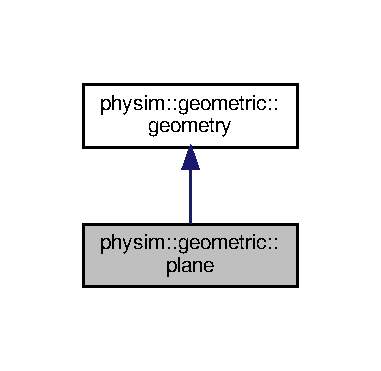
\includegraphics[width=183pt]{classphysim_1_1geometric_1_1plane__inherit__graph}
\end{center}
\end{figure}


Collaboration diagram for physim\+:\+:geometric\+:\+:plane\+:\nopagebreak
\begin{figure}[H]
\begin{center}
\leavevmode
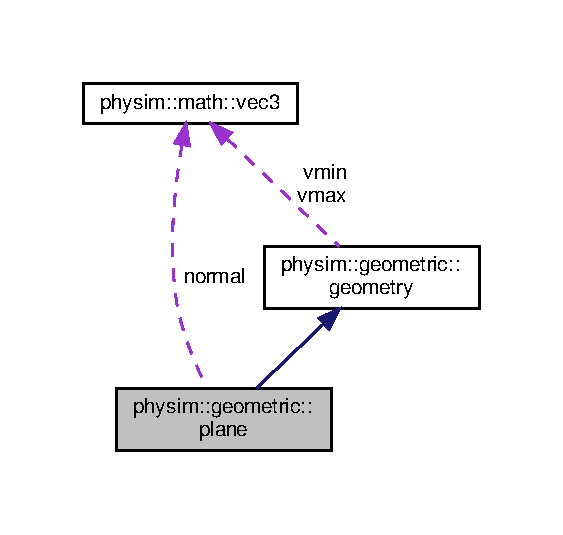
\includegraphics[width=270pt]{classphysim_1_1geometric_1_1plane__coll__graph}
\end{center}
\end{figure}
\subsection*{Public Member Functions}
\begin{DoxyCompactItemize}
\item 
\mbox{\Hypertarget{classphysim_1_1geometric_1_1plane_a984cb3039847ca3c6f899b2bc14b87d7}\label{classphysim_1_1geometric_1_1plane_a984cb3039847ca3c6f899b2bc14b87d7}} 
\hyperlink{classphysim_1_1geometric_1_1plane_a984cb3039847ca3c6f899b2bc14b87d7}{plane} ()
\begin{DoxyCompactList}\small\item\em Default constructor. \end{DoxyCompactList}\item 
\hyperlink{classphysim_1_1geometric_1_1plane_a7ebf0374eab0ff75293894fb45b5fe99}{plane} (const \hyperlink{structphysim_1_1math_1_1vec3}{math\+::vec3} \&n, const \hyperlink{structphysim_1_1math_1_1vec3}{math\+::vec3} \&p)
\begin{DoxyCompactList}\small\item\em Construct a plane with a normal and a point. \end{DoxyCompactList}\item 
\hyperlink{classphysim_1_1geometric_1_1plane_a3888aab8477d2f1e182bef0955b8e351}{plane} (const \hyperlink{structphysim_1_1math_1_1vec3}{math\+::vec3} \&n, float d)
\begin{DoxyCompactList}\small\item\em Construct a plane with a normal and the equation\textquotesingle{}s independent term. \end{DoxyCompactList}\item 
\hyperlink{classphysim_1_1geometric_1_1plane_a5d793dd111e0b7c83c7e11b47c037637}{plane} (const \hyperlink{structphysim_1_1math_1_1vec3}{math\+::vec3} \&p0, const \hyperlink{structphysim_1_1math_1_1vec3}{math\+::vec3} \&p1, const \hyperlink{structphysim_1_1math_1_1vec3}{math\+::vec3} \&p2)
\begin{DoxyCompactList}\small\item\em Construct plane with three points. \end{DoxyCompactList}\item 
\mbox{\Hypertarget{classphysim_1_1geometric_1_1plane_ace21e246bc645de9375a24cb8584e5da}\label{classphysim_1_1geometric_1_1plane_ace21e246bc645de9375a24cb8584e5da}} 
\hyperlink{classphysim_1_1geometric_1_1plane_ace21e246bc645de9375a24cb8584e5da}{plane} (const \hyperlink{classphysim_1_1geometric_1_1plane}{plane} \&p)
\begin{DoxyCompactList}\small\item\em Copy constructor. \end{DoxyCompactList}\item 
\mbox{\Hypertarget{classphysim_1_1geometric_1_1plane_a831003b81a0242d23575a1de6c4745bf}\label{classphysim_1_1geometric_1_1plane_a831003b81a0242d23575a1de6c4745bf}} 
\hyperlink{classphysim_1_1geometric_1_1plane_a831003b81a0242d23575a1de6c4745bf}{$\sim$plane} ()
\begin{DoxyCompactList}\small\item\em Destructor. \end{DoxyCompactList}\item 
void \hyperlink{classphysim_1_1geometric_1_1plane_a201455ce1b4493b02b2f0c14e7d57e71}{set\+\_\+position} (const \hyperlink{structphysim_1_1math_1_1vec3}{math\+::vec3} \&p)
\begin{DoxyCompactList}\small\item\em Sets the position of this plane. \end{DoxyCompactList}\item 
\mbox{\Hypertarget{classphysim_1_1geometric_1_1plane_a857294ae1706c7cfd33cb5b5614b3ac8}\label{classphysim_1_1geometric_1_1plane_a857294ae1706c7cfd33cb5b5614b3ac8}} 
\hyperlink{namespacephysim_1_1geometric_ac2794fff270c5b2ff4307f107a365fca}{geometry\+\_\+type} \hyperlink{classphysim_1_1geometric_1_1plane_a857294ae1706c7cfd33cb5b5614b3ac8}{get\+\_\+geom\+\_\+type} () const
\begin{DoxyCompactList}\small\item\em Returns the type of geometry of this object. \end{DoxyCompactList}\item 
float \hyperlink{classphysim_1_1geometric_1_1plane_ac936ee12c58bf474238f76bb1ad64c2c}{dist\+\_\+point\+\_\+plane} (const \hyperlink{structphysim_1_1math_1_1vec3}{math\+::vec3} \&p) const
\begin{DoxyCompactList}\small\item\em Returns the signed distance between point {\itshape p} and this plane. \end{DoxyCompactList}\item 
\mbox{\Hypertarget{classphysim_1_1geometric_1_1plane_aa734e27be8999129ee2912fc3bb4b0e9}\label{classphysim_1_1geometric_1_1plane_aa734e27be8999129ee2912fc3bb4b0e9}} 
void \hyperlink{classphysim_1_1geometric_1_1plane_aa734e27be8999129ee2912fc3bb4b0e9}{closest\+\_\+point\+\_\+plane} (const \hyperlink{structphysim_1_1math_1_1vec3}{math\+::vec3} \&p, \hyperlink{structphysim_1_1math_1_1vec3}{math\+::vec3} \&c) const
\begin{DoxyCompactList}\small\item\em Returns the project of point {\itshape p} onto the plane. \end{DoxyCompactList}\item 
\mbox{\Hypertarget{classphysim_1_1geometric_1_1plane_a690da5c53e911591de76d487e352049a}\label{classphysim_1_1geometric_1_1plane_a690da5c53e911591de76d487e352049a}} 
const \hyperlink{structphysim_1_1math_1_1vec3}{math\+::vec3} \& \hyperlink{classphysim_1_1geometric_1_1plane_a690da5c53e911591de76d487e352049a}{get\+\_\+normal} () const
\begin{DoxyCompactList}\small\item\em Returns the normal of this plane. \end{DoxyCompactList}\item 
\mbox{\Hypertarget{classphysim_1_1geometric_1_1plane_afe29f5f29c9e9036884747892f17c071}\label{classphysim_1_1geometric_1_1plane_afe29f5f29c9e9036884747892f17c071}} 
float \hyperlink{classphysim_1_1geometric_1_1plane_afe29f5f29c9e9036884747892f17c071}{get\+\_\+constant} () const
\begin{DoxyCompactList}\small\item\em Returns the independent term of this plane\textquotesingle{}s equation. \end{DoxyCompactList}\item 
bool \hyperlink{classphysim_1_1geometric_1_1plane_a873ac41caf2d1ed4b9f8e52502ecbd92}{is\+\_\+inside} (const \hyperlink{structphysim_1_1math_1_1vec3}{math\+::vec3} \&p, float tol=1.e-\/6f) const
\begin{DoxyCompactList}\small\item\em Returns true if {\itshape p} satisfies this plane\textquotesingle{}s equation. \end{DoxyCompactList}\item 
bool \hyperlink{classphysim_1_1geometric_1_1plane_a8a3b99b36271702bbececed5fce16391}{intersec\+\_\+segment} (const \hyperlink{structphysim_1_1math_1_1vec3}{math\+::vec3} \&p1, const \hyperlink{structphysim_1_1math_1_1vec3}{math\+::vec3} \&p2) const
\begin{DoxyCompactList}\small\item\em Returns if the segment defined by the points {\itshape p1} and {\itshape p2} intersects the geometry. \end{DoxyCompactList}\item 
bool \hyperlink{classphysim_1_1geometric_1_1plane_a4e42f4d03045655690ee0339a9f2b50d}{intersec\+\_\+segment} (const \hyperlink{structphysim_1_1math_1_1vec3}{math\+::vec3} \&p1, const \hyperlink{structphysim_1_1math_1_1vec3}{math\+::vec3} \&p2, \hyperlink{structphysim_1_1math_1_1vec3}{math\+::vec3} \&p\+\_\+inter) const
\begin{DoxyCompactList}\small\item\em Returns true if the segment \mbox{[}{\itshape p1}, {\itshape p2} \mbox{]} intersects with the geometry. \end{DoxyCompactList}\item 
bool \hyperlink{classphysim_1_1geometric_1_1plane_a1f4ba9f73933f56201339789e37f7ff7}{intersec\+\_\+sphere} (const \hyperlink{structphysim_1_1math_1_1vec3}{math\+::vec3} \&c, float R) const
\begin{DoxyCompactList}\small\item\em Returns if the sphere with center the point {\itshape c} and radius {\itshape R} intersects the geometry. \end{DoxyCompactList}\item 
void \hyperlink{classphysim_1_1geometric_1_1plane_a9dc212ff39713d1525550c0bf328fe3a}{update\+\_\+particle} (const \hyperlink{structphysim_1_1math_1_1vec3}{math\+::vec3} \&pp, const \hyperlink{structphysim_1_1math_1_1vec3}{math\+::vec3} \&pv, \hyperlink{classphysim_1_1particles_1_1free__particle}{particles\+::free\+\_\+particle} \&p) const
\begin{DoxyCompactList}\small\item\em Update a free particle in a collision with geometry. \end{DoxyCompactList}\item 
void \hyperlink{classphysim_1_1geometric_1_1plane_aff9bd840500b32eeefb89ac0a7d9b95f}{update\+\_\+particle} (const \hyperlink{structphysim_1_1math_1_1vec3}{math\+::vec3} \&pp, const \hyperlink{structphysim_1_1math_1_1vec3}{math\+::vec3} \&pv, \hyperlink{classphysim_1_1particles_1_1sized__particle}{particles\+::sized\+\_\+particle} \&p) const
\begin{DoxyCompactList}\small\item\em Update a sized particle in a collision with geometry. \end{DoxyCompactList}\item 
\mbox{\Hypertarget{classphysim_1_1geometric_1_1plane_a97242bc1446bdfc8fa02f12494249f1e}\label{classphysim_1_1geometric_1_1plane_a97242bc1446bdfc8fa02f12494249f1e}} 
void \hyperlink{classphysim_1_1geometric_1_1plane_a97242bc1446bdfc8fa02f12494249f1e}{display} () const
\begin{DoxyCompactList}\small\item\em Output on stream {\itshape cout} information about this geometry. \end{DoxyCompactList}\end{DoxyCompactItemize}
\subsection*{Private Attributes}
\begin{DoxyCompactItemize}
\item 
\hyperlink{structphysim_1_1math_1_1vec3}{math\+::vec3} \hyperlink{classphysim_1_1geometric_1_1plane_a373cd794f689cf83458f6c6f051b59d9}{normal}
\begin{DoxyCompactList}\small\item\em Normal of the plane. \end{DoxyCompactList}\item 
\mbox{\Hypertarget{classphysim_1_1geometric_1_1plane_a940e09edec2fddf9b8de42d6f6826c1f}\label{classphysim_1_1geometric_1_1plane_a940e09edec2fddf9b8de42d6f6826c1f}} 
float \hyperlink{classphysim_1_1geometric_1_1plane_a940e09edec2fddf9b8de42d6f6826c1f}{dconst}
\begin{DoxyCompactList}\small\item\em Constant, independent term of the plane equation. \end{DoxyCompactList}\end{DoxyCompactItemize}
\subsection*{Additional Inherited Members}


\subsection{Detailed Description}
Class that implements a plane. 

A plane is defined with a normal, unit vector (see \hyperlink{classphysim_1_1geometric_1_1plane_a373cd794f689cf83458f6c6f051b59d9}{normal}) and a constant term (see \hyperlink{classphysim_1_1geometric_1_1plane_a940e09edec2fddf9b8de42d6f6826c1f}{dconst}).

A plane can be defined only with these two parameters (see \hyperlink{classphysim_1_1geometric_1_1plane_a7ebf0374eab0ff75293894fb45b5fe99}{plane(const math\+::vec3\&, const math\+::vec3\&)} or with three points (see \hyperlink{classphysim_1_1geometric_1_1plane_a5d793dd111e0b7c83c7e11b47c037637}{plane(const math\+::vec3\&, const math\+::vec3\&, const math\+::vec3\&)}). 

\subsection{Constructor \& Destructor Documentation}
\mbox{\Hypertarget{classphysim_1_1geometric_1_1plane_a7ebf0374eab0ff75293894fb45b5fe99}\label{classphysim_1_1geometric_1_1plane_a7ebf0374eab0ff75293894fb45b5fe99}} 
\index{physim\+::geometric\+::plane@{physim\+::geometric\+::plane}!plane@{plane}}
\index{plane@{plane}!physim\+::geometric\+::plane@{physim\+::geometric\+::plane}}
\subsubsection{\texorpdfstring{plane()}{plane()}\hspace{0.1cm}{\footnotesize\ttfamily [1/3]}}
{\footnotesize\ttfamily physim\+::geometric\+::plane\+::plane (\begin{DoxyParamCaption}\item[{const \hyperlink{structphysim_1_1math_1_1vec3}{math\+::vec3} \&}]{n,  }\item[{const \hyperlink{structphysim_1_1math_1_1vec3}{math\+::vec3} \&}]{p }\end{DoxyParamCaption})}



Construct a plane with a normal and a point. 


\begin{DoxyParams}{Parameters}
{\em n} & Normal vector of the plane. \\
\hline
{\em p} & Point. \\
\hline
\end{DoxyParams}
\begin{DoxyPostcond}{Postcondition}
\hyperlink{classphysim_1_1geometric_1_1plane_a373cd794f689cf83458f6c6f051b59d9}{normal} takes the normalisation of the vector {\itshape n}. 
\end{DoxyPostcond}
\mbox{\Hypertarget{classphysim_1_1geometric_1_1plane_a3888aab8477d2f1e182bef0955b8e351}\label{classphysim_1_1geometric_1_1plane_a3888aab8477d2f1e182bef0955b8e351}} 
\index{physim\+::geometric\+::plane@{physim\+::geometric\+::plane}!plane@{plane}}
\index{plane@{plane}!physim\+::geometric\+::plane@{physim\+::geometric\+::plane}}
\subsubsection{\texorpdfstring{plane()}{plane()}\hspace{0.1cm}{\footnotesize\ttfamily [2/3]}}
{\footnotesize\ttfamily physim\+::geometric\+::plane\+::plane (\begin{DoxyParamCaption}\item[{const \hyperlink{structphysim_1_1math_1_1vec3}{math\+::vec3} \&}]{n,  }\item[{float}]{d }\end{DoxyParamCaption})}



Construct a plane with a normal and the equation\textquotesingle{}s independent term. 

The plane\textquotesingle{}s equation is $ n \cdot X + d = 0$. 
\begin{DoxyParams}{Parameters}
{\em n} & Normal vector of the plane. \\
\hline
{\em d} & Independent term of the plane\textquotesingle{}s equation. \\
\hline
\end{DoxyParams}
\begin{DoxyPostcond}{Postcondition}
\hyperlink{classphysim_1_1geometric_1_1plane_a373cd794f689cf83458f6c6f051b59d9}{normal} takes the normalisation of the vector {\itshape n}. 
\end{DoxyPostcond}
\mbox{\Hypertarget{classphysim_1_1geometric_1_1plane_a5d793dd111e0b7c83c7e11b47c037637}\label{classphysim_1_1geometric_1_1plane_a5d793dd111e0b7c83c7e11b47c037637}} 
\index{physim\+::geometric\+::plane@{physim\+::geometric\+::plane}!plane@{plane}}
\index{plane@{plane}!physim\+::geometric\+::plane@{physim\+::geometric\+::plane}}
\subsubsection{\texorpdfstring{plane()}{plane()}\hspace{0.1cm}{\footnotesize\ttfamily [3/3]}}
{\footnotesize\ttfamily physim\+::geometric\+::plane\+::plane (\begin{DoxyParamCaption}\item[{const \hyperlink{structphysim_1_1math_1_1vec3}{math\+::vec3} \&}]{p0,  }\item[{const \hyperlink{structphysim_1_1math_1_1vec3}{math\+::vec3} \&}]{p1,  }\item[{const \hyperlink{structphysim_1_1math_1_1vec3}{math\+::vec3} \&}]{p2 }\end{DoxyParamCaption})}



Construct plane with three points. 

The normal of the plane is defined as the cross product of the vectors from {\itshape p0} to {\itshape p1} and from {\itshape p0} to {\itshape p2\+:} $n = ( (p1 - p0) \times (p2 - p0) )/||(p1 - p0) \times (p2 - p0)|| $. 

\subsection{Member Function Documentation}
\mbox{\Hypertarget{classphysim_1_1geometric_1_1plane_ac936ee12c58bf474238f76bb1ad64c2c}\label{classphysim_1_1geometric_1_1plane_ac936ee12c58bf474238f76bb1ad64c2c}} 
\index{physim\+::geometric\+::plane@{physim\+::geometric\+::plane}!dist\+\_\+point\+\_\+plane@{dist\+\_\+point\+\_\+plane}}
\index{dist\+\_\+point\+\_\+plane@{dist\+\_\+point\+\_\+plane}!physim\+::geometric\+::plane@{physim\+::geometric\+::plane}}
\subsubsection{\texorpdfstring{dist\+\_\+point\+\_\+plane()}{dist\_point\_plane()}}
{\footnotesize\ttfamily float physim\+::geometric\+::plane\+::dist\+\_\+point\+\_\+plane (\begin{DoxyParamCaption}\item[{const \hyperlink{structphysim_1_1math_1_1vec3}{math\+::vec3} \&}]{p }\end{DoxyParamCaption}) const}



Returns the signed distance between point {\itshape p} and this plane. 


\begin{DoxyParams}{Parameters}
{\em p} & Point \\
\hline
\end{DoxyParams}
\begin{DoxyReturn}{Returns}
Returns a positive distance if the point {\itshape p} is at the \textquotesingle{}positive\textquotesingle{} side of the plane, and a negative distance if the point {\itshape p} is at the \textquotesingle{}negative\textquotesingle{} side of the plane.~\newline
The positive side is that halfspace such that all the points $q$ belonging to it are such that $ q\cdot n + d > 0$, where $n,d$ are the normal vector and the constant term, respectively, of this plane. 
\end{DoxyReturn}
\mbox{\Hypertarget{classphysim_1_1geometric_1_1plane_a8a3b99b36271702bbececed5fce16391}\label{classphysim_1_1geometric_1_1plane_a8a3b99b36271702bbececed5fce16391}} 
\index{physim\+::geometric\+::plane@{physim\+::geometric\+::plane}!intersec\+\_\+segment@{intersec\+\_\+segment}}
\index{intersec\+\_\+segment@{intersec\+\_\+segment}!physim\+::geometric\+::plane@{physim\+::geometric\+::plane}}
\subsubsection{\texorpdfstring{intersec\+\_\+segment()}{intersec\_segment()}\hspace{0.1cm}{\footnotesize\ttfamily [1/2]}}
{\footnotesize\ttfamily bool physim\+::geometric\+::plane\+::intersec\+\_\+segment (\begin{DoxyParamCaption}\item[{const \hyperlink{structphysim_1_1math_1_1vec3}{math\+::vec3} \&}]{p1,  }\item[{const \hyperlink{structphysim_1_1math_1_1vec3}{math\+::vec3} \&}]{p2 }\end{DoxyParamCaption}) const\hspace{0.3cm}{\ttfamily [virtual]}}



Returns if the segment defined by the points {\itshape p1} and {\itshape p2} intersects the geometry. 


\begin{DoxyParams}[1]{Parameters}
\mbox{\tt in}  & {\em p1} & First endpoint of the segment. \\
\hline
\mbox{\tt in}  & {\em p2} & Second endpoint of the segment. \\
\hline
\end{DoxyParams}
\begin{DoxyReturn}{Returns}
Returns true if there is intersection. 
\end{DoxyReturn}


Implements \hyperlink{classphysim_1_1geometric_1_1geometry_a63d63c340937cede50a95903679c5ad3}{physim\+::geometric\+::geometry}.

\mbox{\Hypertarget{classphysim_1_1geometric_1_1plane_a4e42f4d03045655690ee0339a9f2b50d}\label{classphysim_1_1geometric_1_1plane_a4e42f4d03045655690ee0339a9f2b50d}} 
\index{physim\+::geometric\+::plane@{physim\+::geometric\+::plane}!intersec\+\_\+segment@{intersec\+\_\+segment}}
\index{intersec\+\_\+segment@{intersec\+\_\+segment}!physim\+::geometric\+::plane@{physim\+::geometric\+::plane}}
\subsubsection{\texorpdfstring{intersec\+\_\+segment()}{intersec\_segment()}\hspace{0.1cm}{\footnotesize\ttfamily [2/2]}}
{\footnotesize\ttfamily bool physim\+::geometric\+::plane\+::intersec\+\_\+segment (\begin{DoxyParamCaption}\item[{const \hyperlink{structphysim_1_1math_1_1vec3}{math\+::vec3} \&}]{p1,  }\item[{const \hyperlink{structphysim_1_1math_1_1vec3}{math\+::vec3} \&}]{p2,  }\item[{\hyperlink{structphysim_1_1math_1_1vec3}{math\+::vec3} \&}]{p\+\_\+inter }\end{DoxyParamCaption}) const\hspace{0.3cm}{\ttfamily [virtual]}}



Returns true if the segment \mbox{[}{\itshape p1}, {\itshape p2} \mbox{]} intersects with the geometry. 


\begin{DoxyParams}[1]{Parameters}
\mbox{\tt in}  & {\em p1} & The first endpoint of the segment. \\
\hline
\mbox{\tt in}  & {\em p2} & The second endpoint of the segment. \\
\hline
\mbox{\tt out}  & {\em p\+\_\+inter} & The intersection point between the segment and the geometry. \\
\hline
\end{DoxyParams}
\begin{DoxyReturn}{Returns}
Returns true if the segment and the geometry intersect. In this case, the value in {\itshape p\+\_\+inter} will be the intersection point. 
\end{DoxyReturn}


Implements \hyperlink{classphysim_1_1geometric_1_1geometry_ae9fa877e89b7b2693a94d0772561ad9a}{physim\+::geometric\+::geometry}.

\mbox{\Hypertarget{classphysim_1_1geometric_1_1plane_a1f4ba9f73933f56201339789e37f7ff7}\label{classphysim_1_1geometric_1_1plane_a1f4ba9f73933f56201339789e37f7ff7}} 
\index{physim\+::geometric\+::plane@{physim\+::geometric\+::plane}!intersec\+\_\+sphere@{intersec\+\_\+sphere}}
\index{intersec\+\_\+sphere@{intersec\+\_\+sphere}!physim\+::geometric\+::plane@{physim\+::geometric\+::plane}}
\subsubsection{\texorpdfstring{intersec\+\_\+sphere()}{intersec\_sphere()}}
{\footnotesize\ttfamily bool physim\+::geometric\+::plane\+::intersec\+\_\+sphere (\begin{DoxyParamCaption}\item[{const \hyperlink{structphysim_1_1math_1_1vec3}{math\+::vec3} \&}]{c,  }\item[{float}]{R }\end{DoxyParamCaption}) const\hspace{0.3cm}{\ttfamily [virtual]}}



Returns if the sphere with center the point {\itshape c} and radius {\itshape R} intersects the geometry. 


\begin{DoxyParams}[1]{Parameters}
\mbox{\tt in}  & {\em c} & Center of the sphere. \\
\hline
\mbox{\tt in}  & {\em R} & radius of the sphere. \\
\hline
\end{DoxyParams}
\begin{DoxyReturn}{Returns}
Returns true if there is intersection. 
\end{DoxyReturn}


Implements \hyperlink{classphysim_1_1geometric_1_1geometry_aab49e452a72d1ecaf434be2b8de98169}{physim\+::geometric\+::geometry}.

\mbox{\Hypertarget{classphysim_1_1geometric_1_1plane_a873ac41caf2d1ed4b9f8e52502ecbd92}\label{classphysim_1_1geometric_1_1plane_a873ac41caf2d1ed4b9f8e52502ecbd92}} 
\index{physim\+::geometric\+::plane@{physim\+::geometric\+::plane}!is\+\_\+inside@{is\+\_\+inside}}
\index{is\+\_\+inside@{is\+\_\+inside}!physim\+::geometric\+::plane@{physim\+::geometric\+::plane}}
\subsubsection{\texorpdfstring{is\+\_\+inside()}{is\_inside()}}
{\footnotesize\ttfamily bool physim\+::geometric\+::plane\+::is\+\_\+inside (\begin{DoxyParamCaption}\item[{const \hyperlink{structphysim_1_1math_1_1vec3}{math\+::vec3} \&}]{p,  }\item[{float}]{tol = {\ttfamily 1.e-\/6f} }\end{DoxyParamCaption}) const\hspace{0.3cm}{\ttfamily [virtual]}}



Returns true if {\itshape p} satisfies this plane\textquotesingle{}s equation. 

Returns true iff $normal \cdot p + dconst = 0$ where {\itshape normal} is \hyperlink{classphysim_1_1geometric_1_1plane_a373cd794f689cf83458f6c6f051b59d9}{normal} and {\itshape dconst} is \hyperlink{classphysim_1_1geometric_1_1plane_a940e09edec2fddf9b8de42d6f6826c1f}{dconst}.

The equality, however, is satisfied when the left handside of the equation is smaller or equal than {\itshape tol}. 

Implements \hyperlink{classphysim_1_1geometric_1_1geometry_a325d4049d4e14584b389a2f1202bdc08}{physim\+::geometric\+::geometry}.

\mbox{\Hypertarget{classphysim_1_1geometric_1_1plane_a201455ce1b4493b02b2f0c14e7d57e71}\label{classphysim_1_1geometric_1_1plane_a201455ce1b4493b02b2f0c14e7d57e71}} 
\index{physim\+::geometric\+::plane@{physim\+::geometric\+::plane}!set\+\_\+position@{set\+\_\+position}}
\index{set\+\_\+position@{set\+\_\+position}!physim\+::geometric\+::plane@{physim\+::geometric\+::plane}}
\subsubsection{\texorpdfstring{set\+\_\+position()}{set\_position()}}
{\footnotesize\ttfamily void physim\+::geometric\+::plane\+::set\+\_\+position (\begin{DoxyParamCaption}\item[{const \hyperlink{structphysim_1_1math_1_1vec3}{math\+::vec3} \&}]{p }\end{DoxyParamCaption})\hspace{0.3cm}{\ttfamily [virtual]}}



Sets the position of this plane. 

Modifies \hyperlink{classphysim_1_1geometric_1_1plane_a940e09edec2fddf9b8de42d6f6826c1f}{dconst} so that the plane\textquotesingle{}s equation is satisifed by point {\itshape p}. 
\begin{DoxyParams}{Parameters}
{\em p} & Force the plane to go through this point. \\
\hline
\end{DoxyParams}


Implements \hyperlink{classphysim_1_1geometric_1_1geometry_a5b029b5fa8e55847d5aa06b1d341c88c}{physim\+::geometric\+::geometry}.

\mbox{\Hypertarget{classphysim_1_1geometric_1_1plane_a9dc212ff39713d1525550c0bf328fe3a}\label{classphysim_1_1geometric_1_1plane_a9dc212ff39713d1525550c0bf328fe3a}} 
\index{physim\+::geometric\+::plane@{physim\+::geometric\+::plane}!update\+\_\+particle@{update\+\_\+particle}}
\index{update\+\_\+particle@{update\+\_\+particle}!physim\+::geometric\+::plane@{physim\+::geometric\+::plane}}
\subsubsection{\texorpdfstring{update\+\_\+particle()}{update\_particle()}\hspace{0.1cm}{\footnotesize\ttfamily [1/2]}}
{\footnotesize\ttfamily void physim\+::geometric\+::plane\+::update\+\_\+particle (\begin{DoxyParamCaption}\item[{const \hyperlink{structphysim_1_1math_1_1vec3}{math\+::vec3} \&}]{pred\+\_\+pos,  }\item[{const \hyperlink{structphysim_1_1math_1_1vec3}{math\+::vec3} \&}]{pred\+\_\+vel,  }\item[{\hyperlink{classphysim_1_1particles_1_1free__particle}{particles\+::free\+\_\+particle} \&}]{pred }\end{DoxyParamCaption}) const\hspace{0.3cm}{\ttfamily [virtual]}}



Update a free particle in a collision with geometry. 

Assumig that particle {\itshape pred} collided with this geometry, update its position, velocity, ... accordingly.

For example, some geometry may be \textquotesingle{}bouncy\textquotesingle{}, it may give the particle some extra speed. This needs to be updated in this method.

The particle {\itshape pred} is given in a state that is not modified by any solver. That is, the particle\textquotesingle{}s position, velocity, force, ... have the value at time step {\itshape T}. The predicted position and velocity are given in {\itshape pred\+\_\+pos} and {\itshape pred\+\_\+vel}. These are predictions of the position and velocity for time {\itshape T} + {\itshape dt} (where dt is some time step). The modified particle due to the collision must be stored in {\itshape pred}.

This method is called only when it is sure that there has been a collision\+: the segment joining the particle\textquotesingle{}s current position and the predicted position intersects the geometry.


\begin{DoxyParams}[1]{Parameters}
\mbox{\tt in}  & {\em pred\+\_\+pos} & The predicted position of the particle. \\
\hline
\mbox{\tt in}  & {\em pred\+\_\+vel} & The predicted velocity of the particle. \\
\hline
\mbox{\tt out}  & {\em pred} & The particle with the result of the collision. \\
\hline
\end{DoxyParams}


Implements \hyperlink{classphysim_1_1geometric_1_1geometry_ae5d606ba51451b964fcb2301d5622cab}{physim\+::geometric\+::geometry}.

\mbox{\Hypertarget{classphysim_1_1geometric_1_1plane_aff9bd840500b32eeefb89ac0a7d9b95f}\label{classphysim_1_1geometric_1_1plane_aff9bd840500b32eeefb89ac0a7d9b95f}} 
\index{physim\+::geometric\+::plane@{physim\+::geometric\+::plane}!update\+\_\+particle@{update\+\_\+particle}}
\index{update\+\_\+particle@{update\+\_\+particle}!physim\+::geometric\+::plane@{physim\+::geometric\+::plane}}
\subsubsection{\texorpdfstring{update\+\_\+particle()}{update\_particle()}\hspace{0.1cm}{\footnotesize\ttfamily [2/2]}}
{\footnotesize\ttfamily void physim\+::geometric\+::plane\+::update\+\_\+particle (\begin{DoxyParamCaption}\item[{const \hyperlink{structphysim_1_1math_1_1vec3}{math\+::vec3} \&}]{pred\+\_\+pos,  }\item[{const \hyperlink{structphysim_1_1math_1_1vec3}{math\+::vec3} \&}]{pred\+\_\+vel,  }\item[{\hyperlink{classphysim_1_1particles_1_1sized__particle}{particles\+::sized\+\_\+particle} \&}]{pred }\end{DoxyParamCaption}) const\hspace{0.3cm}{\ttfamily [virtual]}}



Update a sized particle in a collision with geometry. 

Assumig that particle {\itshape pred} collided with this geometry, update its position, velocity, ... accordingly.

For example, some geometry may be \textquotesingle{}bouncy\textquotesingle{}, it may give the particle some extra speed. This needs to be updated in this method.

The particle {\itshape pred} is given in a state that is not modified by any solver. That is, the particle\textquotesingle{}s position, velocity, force, ... have the value at time step {\itshape T}. The predicted position and velocity are given in {\itshape pred\+\_\+pos} and {\itshape pred\+\_\+vel}. These are predictions of the position and velocity for time {\itshape T} + {\itshape dt} (where dt is some time step). The modified particle due to the collision must be stored in {\itshape pred}.

This method is called only when it is sure that there has been a collision\+: the segment joining the particle\textquotesingle{}s current position and the predicted position intersects the geometry.


\begin{DoxyParams}[1]{Parameters}
\mbox{\tt in}  & {\em pred\+\_\+pos} & The predicted position of the particle. \\
\hline
\mbox{\tt in}  & {\em pred\+\_\+vel} & The predicted velocity of the particle. \\
\hline
\mbox{\tt out}  & {\em pred} & The particle with the result of the collision. \\
\hline
\end{DoxyParams}


Implements \hyperlink{classphysim_1_1geometric_1_1geometry_a11c26d2fea85bf7bc41ec94cefa9729e}{physim\+::geometric\+::geometry}.



\subsection{Member Data Documentation}
\mbox{\Hypertarget{classphysim_1_1geometric_1_1plane_a373cd794f689cf83458f6c6f051b59d9}\label{classphysim_1_1geometric_1_1plane_a373cd794f689cf83458f6c6f051b59d9}} 
\index{physim\+::geometric\+::plane@{physim\+::geometric\+::plane}!normal@{normal}}
\index{normal@{normal}!physim\+::geometric\+::plane@{physim\+::geometric\+::plane}}
\subsubsection{\texorpdfstring{normal}{normal}}
{\footnotesize\ttfamily \hyperlink{structphysim_1_1math_1_1vec3}{math\+::vec3} physim\+::geometric\+::plane\+::normal\hspace{0.3cm}{\ttfamily [private]}}



Normal of the plane. 

This is a unit vector. 

The documentation for this class was generated from the following files\+:\begin{DoxyCompactItemize}
\item 
physim/geometry/plane.\+hpp\item 
physim/geometry/plane.\+cpp\end{DoxyCompactItemize}

\hypertarget{classphysim_1_1fields_1_1punctual}{}\section{physim\+:\+:fields\+:\+:punctual Class Reference}
\label{classphysim_1_1fields_1_1punctual}\index{physim\+::fields\+::punctual@{physim\+::fields\+::punctual}}


Force field caused by a particle.  




{\ttfamily \#include $<$punctual.\+hpp$>$}



Inheritance diagram for physim\+:\+:fields\+:\+:punctual\+:\nopagebreak
\begin{figure}[H]
\begin{center}
\leavevmode
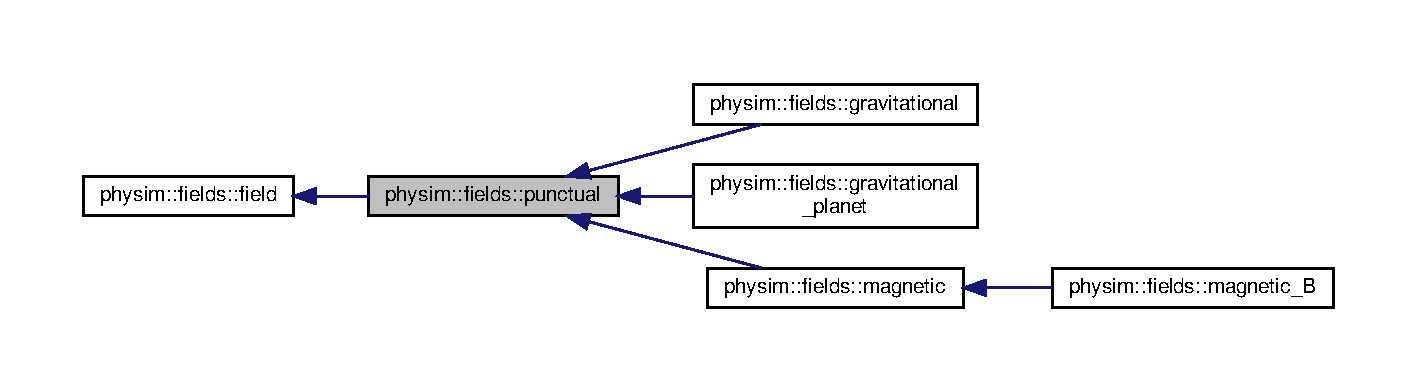
\includegraphics[width=350pt]{classphysim_1_1fields_1_1punctual__inherit__graph}
\end{center}
\end{figure}


Collaboration diagram for physim\+:\+:fields\+:\+:punctual\+:\nopagebreak
\begin{figure}[H]
\begin{center}
\leavevmode
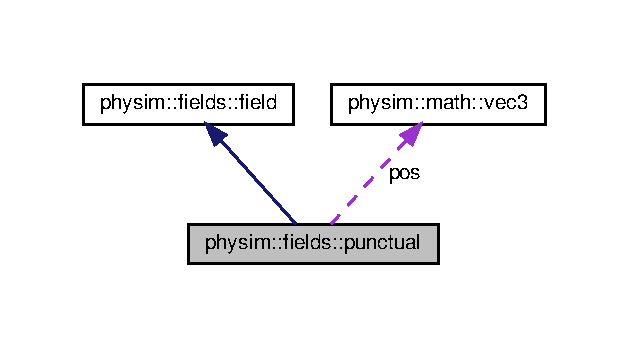
\includegraphics[width=302pt]{classphysim_1_1fields_1_1punctual__coll__graph}
\end{center}
\end{figure}
\subsection*{Public Member Functions}
\begin{DoxyCompactItemize}
\item 
\hyperlink{classphysim_1_1fields_1_1punctual_acd56bc75a1b617501190a427beefbc25}{punctual} ()
\begin{DoxyCompactList}\small\item\em Default constructor. \end{DoxyCompactList}\item 
\mbox{\Hypertarget{classphysim_1_1fields_1_1punctual_ae72780017547f2b39a143e2234e53e60}\label{classphysim_1_1fields_1_1punctual_ae72780017547f2b39a143e2234e53e60}} 
\hyperlink{classphysim_1_1fields_1_1punctual_ae72780017547f2b39a143e2234e53e60}{punctual} (const \hyperlink{structphysim_1_1math_1_1vec3}{math\+::vec3} \&p)
\begin{DoxyCompactList}\small\item\em Constructor with position. \end{DoxyCompactList}\item 
\mbox{\Hypertarget{classphysim_1_1fields_1_1punctual_abb193f2b247fad09ed253ef6ea4a49e9}\label{classphysim_1_1fields_1_1punctual_abb193f2b247fad09ed253ef6ea4a49e9}} 
\hyperlink{classphysim_1_1fields_1_1punctual_abb193f2b247fad09ed253ef6ea4a49e9}{punctual} (const \hyperlink{classphysim_1_1fields_1_1punctual}{punctual} \&f)
\begin{DoxyCompactList}\small\item\em Copy constructor. \end{DoxyCompactList}\item 
\mbox{\Hypertarget{classphysim_1_1fields_1_1punctual_a11079e528b5db0d18336f29c3fad0177}\label{classphysim_1_1fields_1_1punctual_a11079e528b5db0d18336f29c3fad0177}} 
virtual \hyperlink{classphysim_1_1fields_1_1punctual_a11079e528b5db0d18336f29c3fad0177}{$\sim$punctual} ()
\begin{DoxyCompactList}\small\item\em Destructor. \end{DoxyCompactList}\item 
\mbox{\Hypertarget{classphysim_1_1fields_1_1punctual_a3d979184b5ed98a989dcabd7124b7db7}\label{classphysim_1_1fields_1_1punctual_a3d979184b5ed98a989dcabd7124b7db7}} 
void \hyperlink{classphysim_1_1fields_1_1punctual_a3d979184b5ed98a989dcabd7124b7db7}{set\+\_\+position} (const \hyperlink{structphysim_1_1math_1_1vec3}{math\+::vec3} \&p)
\begin{DoxyCompactList}\small\item\em Sets the position of the field. See \hyperlink{classphysim_1_1fields_1_1punctual_a00344d6f3e4f3f841e7d876918c66977}{pos}. \end{DoxyCompactList}\item 
\mbox{\Hypertarget{classphysim_1_1fields_1_1punctual_ac93cc5a07cf093ef1e721237b9340485}\label{classphysim_1_1fields_1_1punctual_ac93cc5a07cf093ef1e721237b9340485}} 
const \hyperlink{structphysim_1_1math_1_1vec3}{math\+::vec3} \& \hyperlink{classphysim_1_1fields_1_1punctual_ac93cc5a07cf093ef1e721237b9340485}{get\+\_\+position} () const
\begin{DoxyCompactList}\small\item\em Returns the position of the field. See \hyperlink{classphysim_1_1fields_1_1punctual_a00344d6f3e4f3f841e7d876918c66977}{pos}. \end{DoxyCompactList}\end{DoxyCompactItemize}
\subsection*{Protected Attributes}
\begin{DoxyCompactItemize}
\item 
\mbox{\Hypertarget{classphysim_1_1fields_1_1punctual_a00344d6f3e4f3f841e7d876918c66977}\label{classphysim_1_1fields_1_1punctual_a00344d6f3e4f3f841e7d876918c66977}} 
\hyperlink{structphysim_1_1math_1_1vec3}{math\+::vec3} \hyperlink{classphysim_1_1fields_1_1punctual_a00344d6f3e4f3f841e7d876918c66977}{pos}
\begin{DoxyCompactList}\small\item\em Center of the field vector. \mbox{[}m\mbox{]}. \end{DoxyCompactList}\end{DoxyCompactItemize}


\subsection{Detailed Description}
Force field caused by a particle. 

\subsection{Constructor \& Destructor Documentation}
\mbox{\Hypertarget{classphysim_1_1fields_1_1punctual_acd56bc75a1b617501190a427beefbc25}\label{classphysim_1_1fields_1_1punctual_acd56bc75a1b617501190a427beefbc25}} 
\index{physim\+::fields\+::punctual@{physim\+::fields\+::punctual}!punctual@{punctual}}
\index{punctual@{punctual}!physim\+::fields\+::punctual@{physim\+::fields\+::punctual}}
\subsubsection{\texorpdfstring{punctual()}{punctual()}}
{\footnotesize\ttfamily physim\+::fields\+::punctual\+::punctual (\begin{DoxyParamCaption}{ }\end{DoxyParamCaption})}



Default constructor. 

Position \hyperlink{classphysim_1_1fields_1_1punctual_a00344d6f3e4f3f841e7d876918c66977}{pos} is initialised at (0,0,0). 

The documentation for this class was generated from the following files\+:\begin{DoxyCompactItemize}
\item 
physim/fields/punctual.\+hpp\item 
physim/fields/punctual.\+cpp\end{DoxyCompactItemize}

\hypertarget{classphysim_1_1emitters_1_1free__emitters_1_1rect__fountain}{}\section{physim\+:\+:emitters\+:\+:free\+\_\+emitters\+:\+:rect\+\_\+fountain Class Reference}
\label{classphysim_1_1emitters_1_1free__emitters_1_1rect__fountain}\index{physim\+::emitters\+::free\+\_\+emitters\+::rect\+\_\+fountain@{physim\+::emitters\+::free\+\_\+emitters\+::rect\+\_\+fountain}}


A fountain emitter.  




{\ttfamily \#include $<$rect\+\_\+fountain.\+hpp$>$}



Inheritance diagram for physim\+:\+:emitters\+:\+:free\+\_\+emitters\+:\+:rect\+\_\+fountain\+:\nopagebreak
\begin{figure}[H]
\begin{center}
\leavevmode
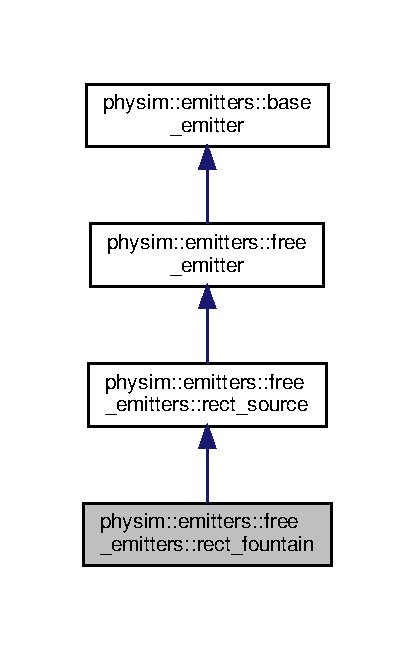
\includegraphics[width=199pt]{classphysim_1_1emitters_1_1free__emitters_1_1rect__fountain__inherit__graph}
\end{center}
\end{figure}


Collaboration diagram for physim\+:\+:emitters\+:\+:free\+\_\+emitters\+:\+:rect\+\_\+fountain\+:\nopagebreak
\begin{figure}[H]
\begin{center}
\leavevmode
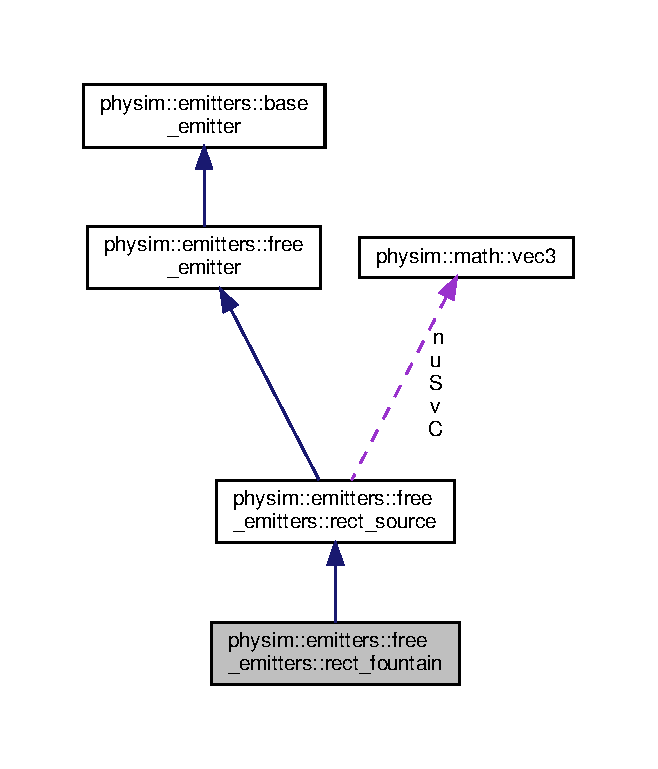
\includegraphics[width=316pt]{classphysim_1_1emitters_1_1free__emitters_1_1rect__fountain__coll__graph}
\end{center}
\end{figure}
\subsection*{Public Member Functions}
\begin{DoxyCompactItemize}
\item 
\mbox{\Hypertarget{classphysim_1_1emitters_1_1free__emitters_1_1rect__fountain_acd9f95ada0c4b401c96d06214e377f36}\label{classphysim_1_1emitters_1_1free__emitters_1_1rect__fountain_acd9f95ada0c4b401c96d06214e377f36}} 
\hyperlink{classphysim_1_1emitters_1_1free__emitters_1_1rect__fountain_acd9f95ada0c4b401c96d06214e377f36}{rect\+\_\+fountain} ()
\begin{DoxyCompactList}\small\item\em Default constructor. \end{DoxyCompactList}\item 
\hyperlink{classphysim_1_1emitters_1_1free__emitters_1_1rect__fountain_a48f4339f6374aa9adbdd1031e1eadb33}{rect\+\_\+fountain} (const \hyperlink{classphysim_1_1emitters_1_1free__emitters_1_1rect__fountain}{rect\+\_\+fountain} \&f)
\begin{DoxyCompactList}\small\item\em Copy constructor. \end{DoxyCompactList}\item 
\mbox{\Hypertarget{classphysim_1_1emitters_1_1free__emitters_1_1rect__fountain_a14e67f38b21eee05cb0fa496d78384e5}\label{classphysim_1_1emitters_1_1free__emitters_1_1rect__fountain_a14e67f38b21eee05cb0fa496d78384e5}} 
\hyperlink{classphysim_1_1emitters_1_1free__emitters_1_1rect__fountain_a14e67f38b21eee05cb0fa496d78384e5}{$\sim$rect\+\_\+fountain} ()
\begin{DoxyCompactList}\small\item\em Destructor. \end{DoxyCompactList}\end{DoxyCompactItemize}
\subsection*{Protected Member Functions}
\begin{DoxyCompactItemize}
\item 
void \hyperlink{classphysim_1_1emitters_1_1free__emitters_1_1rect__fountain_a86c3d792fa977ef2b97785abced613ae}{make\+\_\+vel\+\_\+init} ()
\begin{DoxyCompactList}\small\item\em Sets the velocity initialser. \end{DoxyCompactList}\end{DoxyCompactItemize}
\subsection*{Additional Inherited Members}


\subsection{Detailed Description}
A fountain emitter. 

Provides a position initialiser function so that generated particles behave like a fountain\+: their velocity is set to positive values of the normal to the plane, and values of x and z set as a function of their distance to the center plus some random value.

Need to set the source size through \hyperlink{classphysim_1_1emitters_1_1free__emitters_1_1rect__source_ab85134622163dfc1e3a77730ea94557e}{rect\+\_\+source\+::set\+\_\+rectangular\+\_\+source} method so that the initialser\textquotesingle{}s source is defined. 

\subsection{Constructor \& Destructor Documentation}
\mbox{\Hypertarget{classphysim_1_1emitters_1_1free__emitters_1_1rect__fountain_a48f4339f6374aa9adbdd1031e1eadb33}\label{classphysim_1_1emitters_1_1free__emitters_1_1rect__fountain_a48f4339f6374aa9adbdd1031e1eadb33}} 
\index{physim\+::emitters\+::free\+\_\+emitters\+::rect\+\_\+fountain@{physim\+::emitters\+::free\+\_\+emitters\+::rect\+\_\+fountain}!rect\+\_\+fountain@{rect\+\_\+fountain}}
\index{rect\+\_\+fountain@{rect\+\_\+fountain}!physim\+::emitters\+::free\+\_\+emitters\+::rect\+\_\+fountain@{physim\+::emitters\+::free\+\_\+emitters\+::rect\+\_\+fountain}}
\subsubsection{\texorpdfstring{rect\+\_\+fountain()}{rect\_fountain()}}
{\footnotesize\ttfamily physim\+::emitters\+::free\+\_\+emitters\+::rect\+\_\+fountain\+::rect\+\_\+fountain (\begin{DoxyParamCaption}\item[{const \hyperlink{classphysim_1_1emitters_1_1free__emitters_1_1rect__fountain}{rect\+\_\+fountain} \&}]{f }\end{DoxyParamCaption})}



Copy constructor. 

The function \hyperlink{classphysim_1_1emitters_1_1base__emitter_ac67584a2ca34232c1f4f04c41599df0e}{base\+\_\+emitter\+::pos} is not copied. Instead, it is remade (function \hyperlink{classphysim_1_1emitters_1_1free__emitters_1_1rect__fountain_a86c3d792fa977ef2b97785abced613ae}{make\+\_\+vel\+\_\+init} is called again). 

\subsection{Member Function Documentation}
\mbox{\Hypertarget{classphysim_1_1emitters_1_1free__emitters_1_1rect__fountain_a86c3d792fa977ef2b97785abced613ae}\label{classphysim_1_1emitters_1_1free__emitters_1_1rect__fountain_a86c3d792fa977ef2b97785abced613ae}} 
\index{physim\+::emitters\+::free\+\_\+emitters\+::rect\+\_\+fountain@{physim\+::emitters\+::free\+\_\+emitters\+::rect\+\_\+fountain}!make\+\_\+vel\+\_\+init@{make\+\_\+vel\+\_\+init}}
\index{make\+\_\+vel\+\_\+init@{make\+\_\+vel\+\_\+init}!physim\+::emitters\+::free\+\_\+emitters\+::rect\+\_\+fountain@{physim\+::emitters\+::free\+\_\+emitters\+::rect\+\_\+fountain}}
\subsubsection{\texorpdfstring{make\+\_\+vel\+\_\+init()}{make\_vel\_init()}}
{\footnotesize\ttfamily void physim\+::emitters\+::free\+\_\+emitters\+::rect\+\_\+fountain\+::make\+\_\+vel\+\_\+init (\begin{DoxyParamCaption}{ }\end{DoxyParamCaption})\hspace{0.3cm}{\ttfamily [protected]}, {\ttfamily [virtual]}}



Sets the velocity initialser. 

The velocity is set so that those points that are\+:
\begin{DoxyItemize}
\item farther from the rectangle\textquotesingle{}s center have a smaller-\/magnitude, \char`\"{}flatter\char`\"{} vector velocity, i.\+e., the angle between the vector and the plane is small.
\item closer to the center have larger-\/magnitude and \char`\"{}more vertical\char`\"{} vector velocity, i.\+e., the angle between the vector and the plane is large. 
\end{DoxyItemize}

Implements \hyperlink{classphysim_1_1emitters_1_1free__emitters_1_1rect__source_aace4d8f596f2a138e098ab0f86e927b5}{physim\+::emitters\+::free\+\_\+emitters\+::rect\+\_\+source}.



The documentation for this class was generated from the following files\+:\begin{DoxyCompactItemize}
\item 
physim/emitter/free\+\_\+emitters/rect\+\_\+fountain.\+hpp\item 
physim/emitter/free\+\_\+emitters/rect\+\_\+fountain.\+cpp\end{DoxyCompactItemize}

\hypertarget{classphysim_1_1emitters_1_1free__emitters_1_1rect__shower}{}\section{physim\+:\+:emitters\+:\+:free\+\_\+emitters\+:\+:rect\+\_\+shower Class Reference}
\label{classphysim_1_1emitters_1_1free__emitters_1_1rect__shower}\index{physim\+::emitters\+::free\+\_\+emitters\+::rect\+\_\+shower@{physim\+::emitters\+::free\+\_\+emitters\+::rect\+\_\+shower}}


A shower emitter.  




{\ttfamily \#include $<$rect\+\_\+shower.\+hpp$>$}



Inheritance diagram for physim\+:\+:emitters\+:\+:free\+\_\+emitters\+:\+:rect\+\_\+shower\+:\nopagebreak
\begin{figure}[H]
\begin{center}
\leavevmode
\includegraphics[width=196pt]{classphysim_1_1emitters_1_1free__emitters_1_1rect__shower__inherit__graph}
\end{center}
\end{figure}


Collaboration diagram for physim\+:\+:emitters\+:\+:free\+\_\+emitters\+:\+:rect\+\_\+shower\+:\nopagebreak
\begin{figure}[H]
\begin{center}
\leavevmode
\includegraphics[width=316pt]{classphysim_1_1emitters_1_1free__emitters_1_1rect__shower__coll__graph}
\end{center}
\end{figure}
\subsection*{Public Member Functions}
\begin{DoxyCompactItemize}
\item 
\mbox{\Hypertarget{classphysim_1_1emitters_1_1free__emitters_1_1rect__shower_a7c334dfc7c9192e5f097c198981f28c8}\label{classphysim_1_1emitters_1_1free__emitters_1_1rect__shower_a7c334dfc7c9192e5f097c198981f28c8}} 
\hyperlink{classphysim_1_1emitters_1_1free__emitters_1_1rect__shower_a7c334dfc7c9192e5f097c198981f28c8}{rect\+\_\+shower} ()
\begin{DoxyCompactList}\small\item\em Default constructor. \end{DoxyCompactList}\item 
\mbox{\Hypertarget{classphysim_1_1emitters_1_1free__emitters_1_1rect__shower_af96b9ac048d24aa8fd3dbe61634f371c}\label{classphysim_1_1emitters_1_1free__emitters_1_1rect__shower_af96b9ac048d24aa8fd3dbe61634f371c}} 
\hyperlink{classphysim_1_1emitters_1_1free__emitters_1_1rect__shower_af96b9ac048d24aa8fd3dbe61634f371c}{rect\+\_\+shower} (const \hyperlink{classphysim_1_1emitters_1_1free__emitters_1_1rect__shower}{rect\+\_\+shower} \&\hyperlink{classphysim_1_1emitters_1_1free__emitters_1_1rect__source_ab6e88219088b1048622242f7f2d03f91}{w})
\begin{DoxyCompactList}\small\item\em Copy constructor. \end{DoxyCompactList}\item 
\mbox{\Hypertarget{classphysim_1_1emitters_1_1free__emitters_1_1rect__shower_ab687fca42ff43d5576cccfca4a793c31}\label{classphysim_1_1emitters_1_1free__emitters_1_1rect__shower_ab687fca42ff43d5576cccfca4a793c31}} 
\hyperlink{classphysim_1_1emitters_1_1free__emitters_1_1rect__shower_ab687fca42ff43d5576cccfca4a793c31}{$\sim$rect\+\_\+shower} ()
\begin{DoxyCompactList}\small\item\em Destructor. \end{DoxyCompactList}\item 
\mbox{\Hypertarget{classphysim_1_1emitters_1_1free__emitters_1_1rect__shower_a66ab8bd169b7ff4639214103845e6af9}\label{classphysim_1_1emitters_1_1free__emitters_1_1rect__shower_a66ab8bd169b7ff4639214103845e6af9}} 
\hyperlink{classphysim_1_1emitters_1_1free__emitter}{free\+\_\+emitter} $\ast$ \hyperlink{classphysim_1_1emitters_1_1free__emitters_1_1rect__shower_a66ab8bd169b7ff4639214103845e6af9}{clone} () const
\begin{DoxyCompactList}\small\item\em Returns a reference to a copy of this emitter. \end{DoxyCompactList}\end{DoxyCompactItemize}
\subsection*{Protected Member Functions}
\begin{DoxyCompactItemize}
\item 
void \hyperlink{classphysim_1_1emitters_1_1free__emitters_1_1rect__shower_ab1c7c992c636e3a15e70d6ce3180ed70}{make\+\_\+vel\+\_\+init} ()
\begin{DoxyCompactList}\small\item\em Sets the velocity initialser. \end{DoxyCompactList}\end{DoxyCompactItemize}
\subsection*{Additional Inherited Members}


\subsection{Detailed Description}
A shower emitter. 

Provides a position initialiser function so that generated particles behave like a shower\+: their velocity is set to negative values of y, and null values of x and z.

Need to set the source size through \hyperlink{classphysim_1_1emitters_1_1free__emitters_1_1rect__source_ab85134622163dfc1e3a77730ea94557e}{rect\+\_\+source\+::set\+\_\+rectangular\+\_\+source} method so that the initialser\textquotesingle{}s source is defined. 

\subsection{Member Function Documentation}
\mbox{\Hypertarget{classphysim_1_1emitters_1_1free__emitters_1_1rect__shower_ab1c7c992c636e3a15e70d6ce3180ed70}\label{classphysim_1_1emitters_1_1free__emitters_1_1rect__shower_ab1c7c992c636e3a15e70d6ce3180ed70}} 
\index{physim\+::emitters\+::free\+\_\+emitters\+::rect\+\_\+shower@{physim\+::emitters\+::free\+\_\+emitters\+::rect\+\_\+shower}!make\+\_\+vel\+\_\+init@{make\+\_\+vel\+\_\+init}}
\index{make\+\_\+vel\+\_\+init@{make\+\_\+vel\+\_\+init}!physim\+::emitters\+::free\+\_\+emitters\+::rect\+\_\+shower@{physim\+::emitters\+::free\+\_\+emitters\+::rect\+\_\+shower}}
\subsubsection{\texorpdfstring{make\+\_\+vel\+\_\+init()}{make\_vel\_init()}}
{\footnotesize\ttfamily void physim\+::emitters\+::free\+\_\+emitters\+::rect\+\_\+shower\+::make\+\_\+vel\+\_\+init (\begin{DoxyParamCaption}{ }\end{DoxyParamCaption})\hspace{0.3cm}{\ttfamily [protected]}, {\ttfamily [virtual]}}



Sets the velocity initialser. 

The velocity is set to negative values of y, and null values of x and z. 

Implements \hyperlink{classphysim_1_1emitters_1_1free__emitters_1_1rect__source_aace4d8f596f2a138e098ab0f86e927b5}{physim\+::emitters\+::free\+\_\+emitters\+::rect\+\_\+source}.



The documentation for this class was generated from the following files\+:\begin{DoxyCompactItemize}
\item 
physim/emitter/free\+\_\+emitters/rect\+\_\+shower.\+hpp\item 
physim/emitter/free\+\_\+emitters/rect\+\_\+shower.\+cpp\end{DoxyCompactItemize}

\hypertarget{classphysim_1_1emitters_1_1free__emitters_1_1rect__source}{}\section{physim\+:\+:emitters\+:\+:free\+\_\+emitters\+:\+:rect\+\_\+source Class Reference}
\label{classphysim_1_1emitters_1_1free__emitters_1_1rect__source}\index{physim\+::emitters\+::free\+\_\+emitters\+::rect\+\_\+source@{physim\+::emitters\+::free\+\_\+emitters\+::rect\+\_\+source}}


A rectangular emitter.  




{\ttfamily \#include $<$rect\+\_\+source.\+hpp$>$}



Inheritance diagram for physim\+:\+:emitters\+:\+:free\+\_\+emitters\+:\+:rect\+\_\+source\+:\nopagebreak
\begin{figure}[H]
\begin{center}
\leavevmode
\includegraphics[width=350pt]{classphysim_1_1emitters_1_1free__emitters_1_1rect__source__inherit__graph}
\end{center}
\end{figure}


Collaboration diagram for physim\+:\+:emitters\+:\+:free\+\_\+emitters\+:\+:rect\+\_\+source\+:\nopagebreak
\begin{figure}[H]
\begin{center}
\leavevmode
\includegraphics[width=316pt]{classphysim_1_1emitters_1_1free__emitters_1_1rect__source__coll__graph}
\end{center}
\end{figure}
\subsection*{Public Member Functions}
\begin{DoxyCompactItemize}
\item 
\mbox{\Hypertarget{classphysim_1_1emitters_1_1free__emitters_1_1rect__source_aaeb94fe15698d716f7d3641f0d6365bf}\label{classphysim_1_1emitters_1_1free__emitters_1_1rect__source_aaeb94fe15698d716f7d3641f0d6365bf}} 
\hyperlink{classphysim_1_1emitters_1_1free__emitters_1_1rect__source_aaeb94fe15698d716f7d3641f0d6365bf}{rect\+\_\+source} ()
\begin{DoxyCompactList}\small\item\em Default constructor. \end{DoxyCompactList}\item 
\hyperlink{classphysim_1_1emitters_1_1free__emitters_1_1rect__source_a2aa2b82ecb8b46f6a5cda7c8b19f8f05}{rect\+\_\+source} (const \hyperlink{classphysim_1_1emitters_1_1free__emitters_1_1rect__source}{rect\+\_\+source} \&rs)
\begin{DoxyCompactList}\small\item\em Copy constructor. \end{DoxyCompactList}\item 
\mbox{\Hypertarget{classphysim_1_1emitters_1_1free__emitters_1_1rect__source_aa3447fb2fe83b0b4c80ea30ef45882a2}\label{classphysim_1_1emitters_1_1free__emitters_1_1rect__source_aa3447fb2fe83b0b4c80ea30ef45882a2}} 
virtual \hyperlink{classphysim_1_1emitters_1_1free__emitters_1_1rect__source_aa3447fb2fe83b0b4c80ea30ef45882a2}{$\sim$rect\+\_\+source} ()
\begin{DoxyCompactList}\small\item\em Destructor. \end{DoxyCompactList}\item 
void \hyperlink{classphysim_1_1emitters_1_1free__emitters_1_1rect__source_ab85134622163dfc1e3a77730ea94557e}{set\+\_\+rectangular\+\_\+source} (const \hyperlink{structphysim_1_1math_1_1vec3}{math\+::vec3} \&\+\_\+S, const \hyperlink{structphysim_1_1math_1_1vec3}{math\+::vec3} \&\+\_\+u, const \hyperlink{structphysim_1_1math_1_1vec3}{math\+::vec3} \&\+\_\+v, float \+\_\+w, float \+\_\+h)
\begin{DoxyCompactList}\small\item\em Sets the source of the rectangle. \end{DoxyCompactList}\item 
void \hyperlink{classphysim_1_1emitters_1_1free__emitters_1_1rect__source_a815c63a97fe9fd5defe9110666e4c794}{set\+\_\+straight\+\_\+source} (const \hyperlink{structphysim_1_1math_1_1vec3}{math\+::vec3} \&\+\_\+S, float \+\_\+w, float \+\_\+h)
\begin{DoxyCompactList}\small\item\em Patricular case of flat rectangular source. \end{DoxyCompactList}\item 
\mbox{\Hypertarget{classphysim_1_1emitters_1_1free__emitters_1_1rect__source_a629b14b434936e5dfd1f82ac6e7853a8}\label{classphysim_1_1emitters_1_1free__emitters_1_1rect__source_a629b14b434936e5dfd1f82ac6e7853a8}} 
virtual \hyperlink{classphysim_1_1emitters_1_1free__emitter}{free\+\_\+emitter} $\ast$ \hyperlink{classphysim_1_1emitters_1_1free__emitters_1_1rect__source_a629b14b434936e5dfd1f82ac6e7853a8}{clone} () const =0
\begin{DoxyCompactList}\small\item\em Returns a reference to a copy of this emitter. \end{DoxyCompactList}\end{DoxyCompactItemize}
\subsection*{Protected Member Functions}
\begin{DoxyCompactItemize}
\item 
virtual void \hyperlink{classphysim_1_1emitters_1_1free__emitters_1_1rect__source_ab5109666862f8f49e18f06d9bf663901}{make\+\_\+pos\+\_\+init} ()
\begin{DoxyCompactList}\small\item\em Sets the position initialser. \end{DoxyCompactList}\item 
virtual void \hyperlink{classphysim_1_1emitters_1_1free__emitters_1_1rect__source_aace4d8f596f2a138e098ab0f86e927b5}{make\+\_\+vel\+\_\+init} ()=0
\begin{DoxyCompactList}\small\item\em Sets the velocity initialser. \end{DoxyCompactList}\end{DoxyCompactItemize}
\subsection*{Protected Attributes}
\begin{DoxyCompactItemize}
\item 
\mbox{\Hypertarget{classphysim_1_1emitters_1_1free__emitters_1_1rect__source_a3b849dcdb1584ec1fd564d9341ed89f0}\label{classphysim_1_1emitters_1_1free__emitters_1_1rect__source_a3b849dcdb1584ec1fd564d9341ed89f0}} 
std\+::default\+\_\+random\+\_\+engine \hyperlink{classphysim_1_1emitters_1_1free__emitters_1_1rect__source_a3b849dcdb1584ec1fd564d9341ed89f0}{E}
\begin{DoxyCompactList}\small\item\em Engine used in the uniform distribution \hyperlink{classphysim_1_1emitters_1_1free__emitters_1_1rect__source_ad88b5ea9f44837663c5dc53affde853c}{U01}. \end{DoxyCompactList}\item 
\mbox{\Hypertarget{classphysim_1_1emitters_1_1free__emitters_1_1rect__source_ad88b5ea9f44837663c5dc53affde853c}\label{classphysim_1_1emitters_1_1free__emitters_1_1rect__source_ad88b5ea9f44837663c5dc53affde853c}} 
std\+::uniform\+\_\+real\+\_\+distribution$<$ float $>$ \hyperlink{classphysim_1_1emitters_1_1free__emitters_1_1rect__source_ad88b5ea9f44837663c5dc53affde853c}{U01}
\begin{DoxyCompactList}\small\item\em Random number generator for uniform values between 0 and 1. \end{DoxyCompactList}\item 
\mbox{\Hypertarget{classphysim_1_1emitters_1_1free__emitters_1_1rect__source_a0d958945449e9d31e95b154f942b21ca}\label{classphysim_1_1emitters_1_1free__emitters_1_1rect__source_a0d958945449e9d31e95b154f942b21ca}} 
\hyperlink{structphysim_1_1math_1_1vec3}{math\+::vec3} \hyperlink{classphysim_1_1emitters_1_1free__emitters_1_1rect__source_a0d958945449e9d31e95b154f942b21ca}{S}
\begin{DoxyCompactList}\small\item\em The source point of the rectangle. \end{DoxyCompactList}\item 
\mbox{\Hypertarget{classphysim_1_1emitters_1_1free__emitters_1_1rect__source_a06ebfb60a14d8495e495818378aaa519}\label{classphysim_1_1emitters_1_1free__emitters_1_1rect__source_a06ebfb60a14d8495e495818378aaa519}} 
\hyperlink{structphysim_1_1math_1_1vec3}{math\+::vec3} \hyperlink{classphysim_1_1emitters_1_1free__emitters_1_1rect__source_a06ebfb60a14d8495e495818378aaa519}{C}
\begin{DoxyCompactList}\small\item\em The center of the rectangle. \end{DoxyCompactList}\item 
\mbox{\Hypertarget{classphysim_1_1emitters_1_1free__emitters_1_1rect__source_a692e4b1fd9e74b5c7692cad3f0c184c4}\label{classphysim_1_1emitters_1_1free__emitters_1_1rect__source_a692e4b1fd9e74b5c7692cad3f0c184c4}} 
\hyperlink{structphysim_1_1math_1_1vec3}{math\+::vec3} \hyperlink{classphysim_1_1emitters_1_1free__emitters_1_1rect__source_a692e4b1fd9e74b5c7692cad3f0c184c4}{u}
\begin{DoxyCompactList}\small\item\em Unitary vector along the width. \end{DoxyCompactList}\item 
\mbox{\Hypertarget{classphysim_1_1emitters_1_1free__emitters_1_1rect__source_a9540156884818d3f6b0ed86a1b0902d0}\label{classphysim_1_1emitters_1_1free__emitters_1_1rect__source_a9540156884818d3f6b0ed86a1b0902d0}} 
\hyperlink{structphysim_1_1math_1_1vec3}{math\+::vec3} \hyperlink{classphysim_1_1emitters_1_1free__emitters_1_1rect__source_a9540156884818d3f6b0ed86a1b0902d0}{v}
\begin{DoxyCompactList}\small\item\em Unitary vector along the height. \end{DoxyCompactList}\item 
\hyperlink{structphysim_1_1math_1_1vec3}{math\+::vec3} \hyperlink{classphysim_1_1emitters_1_1free__emitters_1_1rect__source_a0ce1fc34b505b94cdbc22cdb05047142}{n}
\begin{DoxyCompactList}\small\item\em Normal to the rectangle. \end{DoxyCompactList}\item 
\mbox{\Hypertarget{classphysim_1_1emitters_1_1free__emitters_1_1rect__source_ab6e88219088b1048622242f7f2d03f91}\label{classphysim_1_1emitters_1_1free__emitters_1_1rect__source_ab6e88219088b1048622242f7f2d03f91}} 
float \hyperlink{classphysim_1_1emitters_1_1free__emitters_1_1rect__source_ab6e88219088b1048622242f7f2d03f91}{w}
\begin{DoxyCompactList}\small\item\em The distance between \hyperlink{classphysim_1_1emitters_1_1free__emitters_1_1rect__source_a0d958945449e9d31e95b154f942b21ca}{S} and the farthest point in $R(\lambda,0)$. \end{DoxyCompactList}\item 
\mbox{\Hypertarget{classphysim_1_1emitters_1_1free__emitters_1_1rect__source_aebabbc2dc4e697b10d37e54d998f1146}\label{classphysim_1_1emitters_1_1free__emitters_1_1rect__source_aebabbc2dc4e697b10d37e54d998f1146}} 
float \hyperlink{classphysim_1_1emitters_1_1free__emitters_1_1rect__source_aebabbc2dc4e697b10d37e54d998f1146}{h}
\begin{DoxyCompactList}\small\item\em The distance between \hyperlink{classphysim_1_1emitters_1_1free__emitters_1_1rect__source_a0d958945449e9d31e95b154f942b21ca}{S} and the farthest point in $R(0,\mu)$. \end{DoxyCompactList}\end{DoxyCompactItemize}


\subsection{Detailed Description}
A rectangular emitter. 

Provides a position initialiser function so that particles are generated within a rectangle of specific dimensions.

Need to set the source size through \hyperlink{classphysim_1_1emitters_1_1free__emitters_1_1rect__source_ab85134622163dfc1e3a77730ea94557e}{set\+\_\+rectangular\+\_\+source} so that the initialser\textquotesingle{}s source is defined. In this method is specified the coordinates of one of its corners (the source \hyperlink{classphysim_1_1emitters_1_1free__emitters_1_1rect__source_a0d958945449e9d31e95b154f942b21ca}{S}), the two unit vectors spanning the plane it belongs to (see \hyperlink{classphysim_1_1emitters_1_1free__emitters_1_1rect__source_a692e4b1fd9e74b5c7692cad3f0c184c4}{u} and \hyperlink{classphysim_1_1emitters_1_1free__emitters_1_1rect__source_a9540156884818d3f6b0ed86a1b0902d0}{v}), and the lengths of the sides, width and length (see \hyperlink{classphysim_1_1emitters_1_1free__emitters_1_1rect__source_aebabbc2dc4e697b10d37e54d998f1146}{h} and \hyperlink{classphysim_1_1emitters_1_1free__emitters_1_1rect__source_ab6e88219088b1048622242f7f2d03f91}{w}).

The points in this rectangle are, then, parametrised by\+:

$R(\lambda, \mu) = S + \lambda\cdot w\cdot \vec{u} + \mu\cdot h\cdot \vec{u}$

for $\lambda,\mu \in [0,1]\subset R$.

Needless to say that if the vectors \hyperlink{classphysim_1_1emitters_1_1free__emitters_1_1rect__source_a692e4b1fd9e74b5c7692cad3f0c184c4}{u} and \hyperlink{classphysim_1_1emitters_1_1free__emitters_1_1rect__source_a9540156884818d3f6b0ed86a1b0902d0}{v} are not perpendicular the result will be a parallelogram, not a rectangle. However, the word \textquotesingle{}rectangle\textquotesingle{} will be used regardless of how misleading it might be. 

\subsection{Constructor \& Destructor Documentation}
\mbox{\Hypertarget{classphysim_1_1emitters_1_1free__emitters_1_1rect__source_a2aa2b82ecb8b46f6a5cda7c8b19f8f05}\label{classphysim_1_1emitters_1_1free__emitters_1_1rect__source_a2aa2b82ecb8b46f6a5cda7c8b19f8f05}} 
\index{physim\+::emitters\+::free\+\_\+emitters\+::rect\+\_\+source@{physim\+::emitters\+::free\+\_\+emitters\+::rect\+\_\+source}!rect\+\_\+source@{rect\+\_\+source}}
\index{rect\+\_\+source@{rect\+\_\+source}!physim\+::emitters\+::free\+\_\+emitters\+::rect\+\_\+source@{physim\+::emitters\+::free\+\_\+emitters\+::rect\+\_\+source}}
\subsubsection{\texorpdfstring{rect\+\_\+source()}{rect\_source()}}
{\footnotesize\ttfamily physim\+::emitters\+::free\+\_\+emitters\+::rect\+\_\+source\+::rect\+\_\+source (\begin{DoxyParamCaption}\item[{const \hyperlink{classphysim_1_1emitters_1_1free__emitters_1_1rect__source}{rect\+\_\+source} \&}]{rs }\end{DoxyParamCaption})}



Copy constructor. 

The function \hyperlink{classphysim_1_1emitters_1_1base__emitter_ac67584a2ca34232c1f4f04c41599df0e}{free\+\_\+emitter\+::pos} is not copied. Instead, it is remade (function \hyperlink{classphysim_1_1emitters_1_1free__emitters_1_1rect__source_ab5109666862f8f49e18f06d9bf663901}{make\+\_\+pos\+\_\+init} is called again). 

\subsection{Member Function Documentation}
\mbox{\Hypertarget{classphysim_1_1emitters_1_1free__emitters_1_1rect__source_ab5109666862f8f49e18f06d9bf663901}\label{classphysim_1_1emitters_1_1free__emitters_1_1rect__source_ab5109666862f8f49e18f06d9bf663901}} 
\index{physim\+::emitters\+::free\+\_\+emitters\+::rect\+\_\+source@{physim\+::emitters\+::free\+\_\+emitters\+::rect\+\_\+source}!make\+\_\+pos\+\_\+init@{make\+\_\+pos\+\_\+init}}
\index{make\+\_\+pos\+\_\+init@{make\+\_\+pos\+\_\+init}!physim\+::emitters\+::free\+\_\+emitters\+::rect\+\_\+source@{physim\+::emitters\+::free\+\_\+emitters\+::rect\+\_\+source}}
\subsubsection{\texorpdfstring{make\+\_\+pos\+\_\+init()}{make\_pos\_init()}}
{\footnotesize\ttfamily void physim\+::emitters\+::free\+\_\+emitters\+::rect\+\_\+source\+::make\+\_\+pos\+\_\+init (\begin{DoxyParamCaption}{ }\end{DoxyParamCaption})\hspace{0.3cm}{\ttfamily [protected]}, {\ttfamily [virtual]}}



Sets the position initialser. 

It is made a virtual function so that this class can be reimplemented in another one.

Positions are generated according to the parametrisation of this rectangle. \mbox{\Hypertarget{classphysim_1_1emitters_1_1free__emitters_1_1rect__source_aace4d8f596f2a138e098ab0f86e927b5}\label{classphysim_1_1emitters_1_1free__emitters_1_1rect__source_aace4d8f596f2a138e098ab0f86e927b5}} 
\index{physim\+::emitters\+::free\+\_\+emitters\+::rect\+\_\+source@{physim\+::emitters\+::free\+\_\+emitters\+::rect\+\_\+source}!make\+\_\+vel\+\_\+init@{make\+\_\+vel\+\_\+init}}
\index{make\+\_\+vel\+\_\+init@{make\+\_\+vel\+\_\+init}!physim\+::emitters\+::free\+\_\+emitters\+::rect\+\_\+source@{physim\+::emitters\+::free\+\_\+emitters\+::rect\+\_\+source}}
\subsubsection{\texorpdfstring{make\+\_\+vel\+\_\+init()}{make\_vel\_init()}}
{\footnotesize\ttfamily virtual void physim\+::emitters\+::free\+\_\+emitters\+::rect\+\_\+source\+::make\+\_\+vel\+\_\+init (\begin{DoxyParamCaption}{ }\end{DoxyParamCaption})\hspace{0.3cm}{\ttfamily [protected]}, {\ttfamily [pure virtual]}}



Sets the velocity initialser. 

It is made a virtual function so that this class can be reimplemented in another one. 

Implemented in \hyperlink{classphysim_1_1emitters_1_1free__emitters_1_1rect__fountain_a86c3d792fa977ef2b97785abced613ae}{physim\+::emitters\+::free\+\_\+emitters\+::rect\+\_\+fountain}, and \hyperlink{classphysim_1_1emitters_1_1free__emitters_1_1rect__shower_ab1c7c992c636e3a15e70d6ce3180ed70}{physim\+::emitters\+::free\+\_\+emitters\+::rect\+\_\+shower}.

\mbox{\Hypertarget{classphysim_1_1emitters_1_1free__emitters_1_1rect__source_ab85134622163dfc1e3a77730ea94557e}\label{classphysim_1_1emitters_1_1free__emitters_1_1rect__source_ab85134622163dfc1e3a77730ea94557e}} 
\index{physim\+::emitters\+::free\+\_\+emitters\+::rect\+\_\+source@{physim\+::emitters\+::free\+\_\+emitters\+::rect\+\_\+source}!set\+\_\+rectangular\+\_\+source@{set\+\_\+rectangular\+\_\+source}}
\index{set\+\_\+rectangular\+\_\+source@{set\+\_\+rectangular\+\_\+source}!physim\+::emitters\+::free\+\_\+emitters\+::rect\+\_\+source@{physim\+::emitters\+::free\+\_\+emitters\+::rect\+\_\+source}}
\subsubsection{\texorpdfstring{set\+\_\+rectangular\+\_\+source()}{set\_rectangular\_source()}}
{\footnotesize\ttfamily void physim\+::emitters\+::free\+\_\+emitters\+::rect\+\_\+source\+::set\+\_\+rectangular\+\_\+source (\begin{DoxyParamCaption}\item[{const \hyperlink{structphysim_1_1math_1_1vec3}{math\+::vec3} \&}]{\+\_\+S,  }\item[{const \hyperlink{structphysim_1_1math_1_1vec3}{math\+::vec3} \&}]{\+\_\+u,  }\item[{const \hyperlink{structphysim_1_1math_1_1vec3}{math\+::vec3} \&}]{\+\_\+v,  }\item[{float}]{\+\_\+w,  }\item[{float}]{\+\_\+h }\end{DoxyParamCaption})}



Sets the source of the rectangle. 

The order of {\itshape \+\_\+u} and {\itshape \+\_\+v} is important. It defines the \textquotesingle{}above\textquotesingle{} and \textquotesingle{}below\textquotesingle{} parts of the rectangle. This is user-\/defined.

The normal (see \hyperlink{classphysim_1_1emitters_1_1free__emitters_1_1rect__source_a0ce1fc34b505b94cdbc22cdb05047142}{n}) is determined as the cross-\/product of \+\_\+u and \+\_\+v, in this order. 
\begin{DoxyParams}{Parameters}
{\em \+\_\+S} & See \hyperlink{classphysim_1_1emitters_1_1free__emitters_1_1rect__source_a0d958945449e9d31e95b154f942b21ca}{S}. \\
\hline
{\em \+\_\+u} & See \hyperlink{classphysim_1_1emitters_1_1free__emitters_1_1rect__source_a692e4b1fd9e74b5c7692cad3f0c184c4}{u}. \\
\hline
{\em \+\_\+v} & See \hyperlink{classphysim_1_1emitters_1_1free__emitters_1_1rect__source_a9540156884818d3f6b0ed86a1b0902d0}{v}. \\
\hline
{\em \+\_\+w} & See \hyperlink{classphysim_1_1emitters_1_1free__emitters_1_1rect__source_ab6e88219088b1048622242f7f2d03f91}{w}. \\
\hline
{\em \+\_\+h} & See \hyperlink{classphysim_1_1emitters_1_1free__emitters_1_1rect__source_aebabbc2dc4e697b10d37e54d998f1146}{h}. \\
\hline
\end{DoxyParams}
\mbox{\Hypertarget{classphysim_1_1emitters_1_1free__emitters_1_1rect__source_a815c63a97fe9fd5defe9110666e4c794}\label{classphysim_1_1emitters_1_1free__emitters_1_1rect__source_a815c63a97fe9fd5defe9110666e4c794}} 
\index{physim\+::emitters\+::free\+\_\+emitters\+::rect\+\_\+source@{physim\+::emitters\+::free\+\_\+emitters\+::rect\+\_\+source}!set\+\_\+straight\+\_\+source@{set\+\_\+straight\+\_\+source}}
\index{set\+\_\+straight\+\_\+source@{set\+\_\+straight\+\_\+source}!physim\+::emitters\+::free\+\_\+emitters\+::rect\+\_\+source@{physim\+::emitters\+::free\+\_\+emitters\+::rect\+\_\+source}}
\subsubsection{\texorpdfstring{set\+\_\+straight\+\_\+source()}{set\_straight\_source()}}
{\footnotesize\ttfamily void physim\+::emitters\+::free\+\_\+emitters\+::rect\+\_\+source\+::set\+\_\+straight\+\_\+source (\begin{DoxyParamCaption}\item[{const \hyperlink{structphysim_1_1math_1_1vec3}{math\+::vec3} \&}]{\+\_\+S,  }\item[{float}]{\+\_\+w,  }\item[{float}]{\+\_\+h }\end{DoxyParamCaption})}



Patricular case of flat rectangular source. 

Unitary vectors used are\+:
\begin{DoxyItemize}
\item \hyperlink{classphysim_1_1emitters_1_1free__emitters_1_1rect__source_a692e4b1fd9e74b5c7692cad3f0c184c4}{u} = (1.\+0, 0.\+0, 0.\+0)
\item \hyperlink{classphysim_1_1emitters_1_1free__emitters_1_1rect__source_a9540156884818d3f6b0ed86a1b0902d0}{v} = (0.\+0, 0.\+0, 1.\+0) 
\begin{DoxyParams}{Parameters}
{\em \+\_\+S} & See \hyperlink{classphysim_1_1emitters_1_1free__emitters_1_1rect__source_a0d958945449e9d31e95b154f942b21ca}{S}. \\
\hline
{\em \+\_\+w} & See \hyperlink{classphysim_1_1emitters_1_1free__emitters_1_1rect__source_ab6e88219088b1048622242f7f2d03f91}{w}. \\
\hline
{\em \+\_\+h} & See \hyperlink{classphysim_1_1emitters_1_1free__emitters_1_1rect__source_aebabbc2dc4e697b10d37e54d998f1146}{h}. \\
\hline
\end{DoxyParams}

\end{DoxyItemize}

\subsection{Member Data Documentation}
\mbox{\Hypertarget{classphysim_1_1emitters_1_1free__emitters_1_1rect__source_a0ce1fc34b505b94cdbc22cdb05047142}\label{classphysim_1_1emitters_1_1free__emitters_1_1rect__source_a0ce1fc34b505b94cdbc22cdb05047142}} 
\index{physim\+::emitters\+::free\+\_\+emitters\+::rect\+\_\+source@{physim\+::emitters\+::free\+\_\+emitters\+::rect\+\_\+source}!n@{n}}
\index{n@{n}!physim\+::emitters\+::free\+\_\+emitters\+::rect\+\_\+source@{physim\+::emitters\+::free\+\_\+emitters\+::rect\+\_\+source}}
\subsubsection{\texorpdfstring{n}{n}}
{\footnotesize\ttfamily \hyperlink{structphysim_1_1math_1_1vec3}{math\+::vec3} physim\+::emitters\+::free\+\_\+emitters\+::rect\+\_\+source\+::n\hspace{0.3cm}{\ttfamily [protected]}}



Normal to the rectangle. 

Unitary vector. Cross-\/product of \hyperlink{classphysim_1_1emitters_1_1free__emitters_1_1rect__source_a692e4b1fd9e74b5c7692cad3f0c184c4}{u} and \hyperlink{classphysim_1_1emitters_1_1free__emitters_1_1rect__source_a9540156884818d3f6b0ed86a1b0902d0}{v}. 

The documentation for this class was generated from the following files\+:\begin{DoxyCompactItemize}
\item 
physim/emitter/free\+\_\+emitters/rect\+\_\+source.\+hpp\item 
physim/emitter/free\+\_\+emitters/rect\+\_\+source.\+cpp\end{DoxyCompactItemize}

\hypertarget{classphysim_1_1geometric_1_1rectangle}{}\section{physim\+:\+:geometric\+:\+:rectangle Class Reference}
\label{classphysim_1_1geometric_1_1rectangle}\index{physim\+::geometric\+::rectangle@{physim\+::geometric\+::rectangle}}


Class that implements a rectangle.  




{\ttfamily \#include $<$rectangle.\+hpp$>$}



Inheritance diagram for physim\+:\+:geometric\+:\+:rectangle\+:\nopagebreak
\begin{figure}[H]
\begin{center}
\leavevmode
\includegraphics[width=183pt]{classphysim_1_1geometric_1_1rectangle__inherit__graph}
\end{center}
\end{figure}


Collaboration diagram for physim\+:\+:geometric\+:\+:rectangle\+:\nopagebreak
\begin{figure}[H]
\begin{center}
\leavevmode
\includegraphics[width=350pt]{classphysim_1_1geometric_1_1rectangle__coll__graph}
\end{center}
\end{figure}
\subsection*{Public Member Functions}
\begin{DoxyCompactItemize}
\item 
\mbox{\Hypertarget{classphysim_1_1geometric_1_1rectangle_a56078b6e9053fffb19e5e5d4648f6880}\label{classphysim_1_1geometric_1_1rectangle_a56078b6e9053fffb19e5e5d4648f6880}} 
\hyperlink{classphysim_1_1geometric_1_1rectangle_a56078b6e9053fffb19e5e5d4648f6880}{rectangle} ()
\begin{DoxyCompactList}\small\item\em Default constructor. \end{DoxyCompactList}\item 
\hyperlink{classphysim_1_1geometric_1_1rectangle_a19ee9fbc0666035eda867de84a7e7df1}{rectangle} (const \hyperlink{structphysim_1_1math_1_1vec3}{math\+::vec3} \&\hyperlink{classphysim_1_1geometric_1_1rectangle_a7af5009a87211214b1b1ef7ec6316d20}{p1}, const \hyperlink{structphysim_1_1math_1_1vec3}{math\+::vec3} \&\hyperlink{classphysim_1_1geometric_1_1rectangle_ab3107a5faeb3c52420ffe4c074a145be}{p2}, const \hyperlink{structphysim_1_1math_1_1vec3}{math\+::vec3} \&\hyperlink{classphysim_1_1geometric_1_1rectangle_a559ad6301b4da2b82350d36cdfa46f23}{p3}, const \hyperlink{structphysim_1_1math_1_1vec3}{math\+::vec3} \&p4)
\begin{DoxyCompactList}\small\item\em Constructor with points. \end{DoxyCompactList}\item 
\mbox{\Hypertarget{classphysim_1_1geometric_1_1rectangle_a46a8abaa08eb338dd25c54afe2cb5044}\label{classphysim_1_1geometric_1_1rectangle_a46a8abaa08eb338dd25c54afe2cb5044}} 
\hyperlink{classphysim_1_1geometric_1_1rectangle_a46a8abaa08eb338dd25c54afe2cb5044}{rectangle} (const \hyperlink{classphysim_1_1geometric_1_1rectangle}{rectangle} \&t)
\begin{DoxyCompactList}\small\item\em Copy constructor. \end{DoxyCompactList}\item 
\mbox{\Hypertarget{classphysim_1_1geometric_1_1rectangle_a5949e485e660adebf4e2d079185a5722}\label{classphysim_1_1geometric_1_1rectangle_a5949e485e660adebf4e2d079185a5722}} 
\hyperlink{classphysim_1_1geometric_1_1rectangle_a5949e485e660adebf4e2d079185a5722}{$\sim$rectangle} ()
\begin{DoxyCompactList}\small\item\em Destructor. \end{DoxyCompactList}\item 
void \hyperlink{classphysim_1_1geometric_1_1rectangle_a55107f7bfff66f8f46392eb5a7a68aae}{set\+\_\+points} (const \hyperlink{structphysim_1_1math_1_1vec3}{math\+::vec3} \&\+\_\+p0, const \hyperlink{structphysim_1_1math_1_1vec3}{math\+::vec3} \&\+\_\+p1, const \hyperlink{structphysim_1_1math_1_1vec3}{math\+::vec3} \&\+\_\+p2, const \hyperlink{structphysim_1_1math_1_1vec3}{math\+::vec3} \&\+\_\+p3)
\begin{DoxyCompactList}\small\item\em Set the points of this rectangle. \end{DoxyCompactList}\item 
void \hyperlink{classphysim_1_1geometric_1_1rectangle_a7458e8b880ace6a3393a728edb6d66fa}{set\+\_\+position} (const \hyperlink{structphysim_1_1math_1_1vec3}{math\+::vec3} \&v)
\begin{DoxyCompactList}\small\item\em Sets the position of this rectangle. \end{DoxyCompactList}\item 
\mbox{\Hypertarget{classphysim_1_1geometric_1_1rectangle_a74d67c86fce1512928a8ce3712c8dc91}\label{classphysim_1_1geometric_1_1rectangle_a74d67c86fce1512928a8ce3712c8dc91}} 
const \hyperlink{classphysim_1_1geometric_1_1plane}{plane} \& \hyperlink{classphysim_1_1geometric_1_1rectangle_a74d67c86fce1512928a8ce3712c8dc91}{get\+\_\+plane} () const
\begin{DoxyCompactList}\small\item\em Returns a constant reference to the assiociated plane (\hyperlink{classphysim_1_1geometric_1_1rectangle_af9c8331b7c76cf77289e08af9b97531e}{pl}). \end{DoxyCompactList}\item 
void \hyperlink{classphysim_1_1geometric_1_1rectangle_a0d5e49e945a8c1a822f7c6c223ce657b}{get\+\_\+points} (\hyperlink{structphysim_1_1math_1_1vec3}{math\+::vec3} \&\+\_\+p0, \hyperlink{structphysim_1_1math_1_1vec3}{math\+::vec3} \&\+\_\+p1, \hyperlink{structphysim_1_1math_1_1vec3}{math\+::vec3} \&\+\_\+p2, \hyperlink{structphysim_1_1math_1_1vec3}{math\+::vec3} \&\+\_\+p3) const
\begin{DoxyCompactList}\small\item\em Return the points of this rectangle. \end{DoxyCompactList}\item 
void \hyperlink{classphysim_1_1geometric_1_1rectangle_a27ae9df28df346dedfbc3500b79123cb}{projection} (const \hyperlink{structphysim_1_1math_1_1vec3}{math\+::vec3} \&p, \hyperlink{structphysim_1_1math_1_1vec3}{math\+::vec3} \&proj) const
\begin{DoxyCompactList}\small\item\em Project a point onto this rectangle. \end{DoxyCompactList}\item 
float \hyperlink{classphysim_1_1geometric_1_1rectangle_a7e80994ff1d2e2be4cdb3f195fc2edef}{distance} (const \hyperlink{structphysim_1_1math_1_1vec3}{math\+::vec3} \&p) const
\begin{DoxyCompactList}\small\item\em Computes the distance between a point and this triangle. \end{DoxyCompactList}\item 
bool \hyperlink{classphysim_1_1geometric_1_1rectangle_ab36400ef3f750fb6482fda8e1044bfa5}{is\+\_\+inside} (const \hyperlink{structphysim_1_1math_1_1vec3}{math\+::vec3} \&p, float tol=1.e-\/6f) const
\begin{DoxyCompactList}\small\item\em Returns whether a point is inside the geometry. \end{DoxyCompactList}\item 
\mbox{\Hypertarget{classphysim_1_1geometric_1_1rectangle_a0113e292a85b730d82a8fb2f417e1f76}\label{classphysim_1_1geometric_1_1rectangle_a0113e292a85b730d82a8fb2f417e1f76}} 
\hyperlink{namespacephysim_1_1geometric_ac2794fff270c5b2ff4307f107a365fca}{geometry\+\_\+type} \hyperlink{classphysim_1_1geometric_1_1rectangle_a0113e292a85b730d82a8fb2f417e1f76}{get\+\_\+geom\+\_\+type} () const
\begin{DoxyCompactList}\small\item\em Returns the type of geometry of this object. \end{DoxyCompactList}\item 
bool \hyperlink{classphysim_1_1geometric_1_1rectangle_aed45b841c7d1e615565e36720386f7a4}{intersec\+\_\+segment} (const \hyperlink{structphysim_1_1math_1_1vec3}{math\+::vec3} \&\+\_\+p1, const \hyperlink{structphysim_1_1math_1_1vec3}{math\+::vec3} \&\+\_\+p2) const
\begin{DoxyCompactList}\small\item\em Returns if the segment defined by the points {\itshape p1} and {\itshape p2} intersects the geometry. \end{DoxyCompactList}\item 
bool \hyperlink{classphysim_1_1geometric_1_1rectangle_a093865345b5a82576351be159ae56ee1}{intersec\+\_\+segment} (const \hyperlink{structphysim_1_1math_1_1vec3}{math\+::vec3} \&\+\_\+p1, const \hyperlink{structphysim_1_1math_1_1vec3}{math\+::vec3} \&\+\_\+p2, \hyperlink{structphysim_1_1math_1_1vec3}{math\+::vec3} \&p\+\_\+inter) const
\begin{DoxyCompactList}\small\item\em Returns true if the segment \mbox{[}{\itshape p1}, {\itshape p2} \mbox{]} intersects with the geometry. \end{DoxyCompactList}\item 
bool \hyperlink{classphysim_1_1geometric_1_1rectangle_a39a293ca40cfbde7a2ef8c1ab487833d}{intersec\+\_\+sphere} (const \hyperlink{structphysim_1_1math_1_1vec3}{math\+::vec3} \&c, float R) const
\begin{DoxyCompactList}\small\item\em Returns if the sphere with center the point {\itshape c} and radius {\itshape R} intersects the geometry. \end{DoxyCompactList}\item 
void \hyperlink{classphysim_1_1geometric_1_1rectangle_a38e4eaa8bff24511cd3a9d94cd04e3dd}{update\+\_\+particle} (const \hyperlink{structphysim_1_1math_1_1vec3}{math\+::vec3} \&pp, const \hyperlink{structphysim_1_1math_1_1vec3}{math\+::vec3} \&pv, \hyperlink{classphysim_1_1particles_1_1free__particle}{particles\+::free\+\_\+particle} \&p) const
\begin{DoxyCompactList}\small\item\em Update a free particle in a collision with geometry. \end{DoxyCompactList}\item 
void \hyperlink{classphysim_1_1geometric_1_1rectangle_a61fead9b22595c9d9be8dc3867e26717}{update\+\_\+particle} (const \hyperlink{structphysim_1_1math_1_1vec3}{math\+::vec3} \&pp, const \hyperlink{structphysim_1_1math_1_1vec3}{math\+::vec3} \&pv, \hyperlink{classphysim_1_1particles_1_1sized__particle}{particles\+::sized\+\_\+particle} \&p) const
\begin{DoxyCompactList}\small\item\em Update a sized particle in a collision with geometry. \end{DoxyCompactList}\item 
\mbox{\Hypertarget{classphysim_1_1geometric_1_1rectangle_a89511cf054316c8f0b6d0adbbf9b511e}\label{classphysim_1_1geometric_1_1rectangle_a89511cf054316c8f0b6d0adbbf9b511e}} 
void \hyperlink{classphysim_1_1geometric_1_1rectangle_a89511cf054316c8f0b6d0adbbf9b511e}{display} () const
\begin{DoxyCompactList}\small\item\em Output on stream {\itshape cout} information about this geometry. \end{DoxyCompactList}\end{DoxyCompactItemize}
\subsection*{Private Attributes}
\begin{DoxyCompactItemize}
\item 
\mbox{\Hypertarget{classphysim_1_1geometric_1_1rectangle_a54ec5f5baaa4cbe0549de696334e46f4}\label{classphysim_1_1geometric_1_1rectangle_a54ec5f5baaa4cbe0549de696334e46f4}} 
\hyperlink{structphysim_1_1math_1_1vec3}{math\+::vec3} \hyperlink{classphysim_1_1geometric_1_1rectangle_a54ec5f5baaa4cbe0549de696334e46f4}{p0}
\begin{DoxyCompactList}\small\item\em The first vertex of the rectangle. \end{DoxyCompactList}\item 
\mbox{\Hypertarget{classphysim_1_1geometric_1_1rectangle_a7af5009a87211214b1b1ef7ec6316d20}\label{classphysim_1_1geometric_1_1rectangle_a7af5009a87211214b1b1ef7ec6316d20}} 
\hyperlink{structphysim_1_1math_1_1vec3}{math\+::vec3} \hyperlink{classphysim_1_1geometric_1_1rectangle_a7af5009a87211214b1b1ef7ec6316d20}{p1}
\begin{DoxyCompactList}\small\item\em The second vertex of the rectangle. \end{DoxyCompactList}\item 
\mbox{\Hypertarget{classphysim_1_1geometric_1_1rectangle_ab3107a5faeb3c52420ffe4c074a145be}\label{classphysim_1_1geometric_1_1rectangle_ab3107a5faeb3c52420ffe4c074a145be}} 
\hyperlink{structphysim_1_1math_1_1vec3}{math\+::vec3} \hyperlink{classphysim_1_1geometric_1_1rectangle_ab3107a5faeb3c52420ffe4c074a145be}{p2}
\begin{DoxyCompactList}\small\item\em The third vertex of the rectangle. \end{DoxyCompactList}\item 
\mbox{\Hypertarget{classphysim_1_1geometric_1_1rectangle_a559ad6301b4da2b82350d36cdfa46f23}\label{classphysim_1_1geometric_1_1rectangle_a559ad6301b4da2b82350d36cdfa46f23}} 
\hyperlink{structphysim_1_1math_1_1vec3}{math\+::vec3} \hyperlink{classphysim_1_1geometric_1_1rectangle_a559ad6301b4da2b82350d36cdfa46f23}{p3}
\begin{DoxyCompactList}\small\item\em The fourth vertex of the rectangle. \end{DoxyCompactList}\item 
\mbox{\Hypertarget{classphysim_1_1geometric_1_1rectangle_af9c8331b7c76cf77289e08af9b97531e}\label{classphysim_1_1geometric_1_1rectangle_af9c8331b7c76cf77289e08af9b97531e}} 
\hyperlink{classphysim_1_1geometric_1_1plane}{plane} \hyperlink{classphysim_1_1geometric_1_1rectangle_af9c8331b7c76cf77289e08af9b97531e}{pl}
\begin{DoxyCompactList}\small\item\em Plane associated to the rectangle. \end{DoxyCompactList}\item 
\hyperlink{structphysim_1_1math_1_1vec3}{math\+::vec3} \hyperlink{classphysim_1_1geometric_1_1rectangle_a09333b95cf8b78186b465a59771f4037}{u0}
\begin{DoxyCompactList}\small\item\em Plane parametrisation vector. \end{DoxyCompactList}\item 
\hyperlink{structphysim_1_1math_1_1vec3}{math\+::vec3} \hyperlink{classphysim_1_1geometric_1_1rectangle_a0570b2c50e93ca033123eaaa00a0e068}{u1}
\begin{DoxyCompactList}\small\item\em Plane parametrisation vector. \end{DoxyCompactList}\item 
\hyperlink{structphysim_1_1math_1_1vec3}{math\+::vec3} \hyperlink{classphysim_1_1geometric_1_1rectangle_a237f0ac5cb92cd71726c5902fb802dc4}{u2}
\begin{DoxyCompactList}\small\item\em Plane parametrisation vector. \end{DoxyCompactList}\item 
\hyperlink{structphysim_1_1math_1_1vec2}{math\+::vec2} \hyperlink{classphysim_1_1geometric_1_1rectangle_a6597a22ccd74d61b3dd0a15585bc1f97}{q0}
\begin{DoxyCompactList}\small\item\em Local reference system point. \end{DoxyCompactList}\item 
\hyperlink{structphysim_1_1math_1_1vec2}{math\+::vec2} \hyperlink{classphysim_1_1geometric_1_1rectangle_adfe3ecd2eeb09b873ea2f619ae799719}{q1}
\begin{DoxyCompactList}\small\item\em Local reference system point. \end{DoxyCompactList}\item 
\hyperlink{structphysim_1_1math_1_1vec2}{math\+::vec2} \hyperlink{classphysim_1_1geometric_1_1rectangle_a43fba2f1112ada230301638e4ec3e3a2}{q2}
\begin{DoxyCompactList}\small\item\em Local reference system point. \end{DoxyCompactList}\item 
\hyperlink{structphysim_1_1math_1_1vec2}{math\+::vec2} \hyperlink{classphysim_1_1geometric_1_1rectangle_abfe5d5c4a309bdd1ab65898c757334e6}{q3}
\begin{DoxyCompactList}\small\item\em Local reference system point. \end{DoxyCompactList}\item 
\hyperlink{structphysim_1_1math_1_1vec2}{math\+::vec2} \hyperlink{classphysim_1_1geometric_1_1rectangle_a70d4839212717247ae294f94cd7de372}{e0}
\begin{DoxyCompactList}\small\item\em Local reference system edge vector. \end{DoxyCompactList}\item 
\hyperlink{structphysim_1_1math_1_1vec2}{math\+::vec2} \hyperlink{classphysim_1_1geometric_1_1rectangle_a511c131352fa83a64f3f30935ae87be7}{e1}
\begin{DoxyCompactList}\small\item\em Local reference system edge vector. \end{DoxyCompactList}\item 
\hyperlink{structphysim_1_1math_1_1vec2}{math\+::vec2} \hyperlink{classphysim_1_1geometric_1_1rectangle_a7d4880bb512b054f354393df0309c2b8}{e2}
\begin{DoxyCompactList}\small\item\em Local reference system edge vector. \end{DoxyCompactList}\item 
\hyperlink{structphysim_1_1math_1_1vec2}{math\+::vec2} \hyperlink{classphysim_1_1geometric_1_1rectangle_a94e615cbf893ff4950e845545796c779}{e3}
\begin{DoxyCompactList}\small\item\em Local reference system edge vector. \end{DoxyCompactList}\item 
\hyperlink{structphysim_1_1math_1_1vec2}{math\+::vec2} \hyperlink{classphysim_1_1geometric_1_1rectangle_a1515a4ffb5dd7bcd8ddc0fbda9eb6564}{n0}
\begin{DoxyCompactList}\small\item\em Local reference system normal edge vector. \end{DoxyCompactList}\item 
\hyperlink{structphysim_1_1math_1_1vec2}{math\+::vec2} \hyperlink{classphysim_1_1geometric_1_1rectangle_a3d075b4865232e66ff9e6d3d60970e1e}{n1}
\begin{DoxyCompactList}\small\item\em Local reference system normal edge vector. \end{DoxyCompactList}\item 
\hyperlink{structphysim_1_1math_1_1vec2}{math\+::vec2} \hyperlink{classphysim_1_1geometric_1_1rectangle_a0f79adf34a89ed7d8033aa1ad037ba2f}{n2}
\begin{DoxyCompactList}\small\item\em Local reference system normal edge vector. \end{DoxyCompactList}\item 
\hyperlink{structphysim_1_1math_1_1vec2}{math\+::vec2} \hyperlink{classphysim_1_1geometric_1_1rectangle_a225b6af98f7ce91c6b0f4fc1aee25f72}{n3}
\begin{DoxyCompactList}\small\item\em Local reference system normal edge vector. \end{DoxyCompactList}\item 
\hyperlink{structphysim_1_1math_1_1vec2}{math\+::vec2} \hyperlink{classphysim_1_1geometric_1_1rectangle_a6643ef4e07ab484fa12dc9e323729313}{q0n0}
\begin{DoxyCompactList}\small\item\em Local reference system normal edge point. \end{DoxyCompactList}\item 
\hyperlink{structphysim_1_1math_1_1vec2}{math\+::vec2} \hyperlink{classphysim_1_1geometric_1_1rectangle_a8d187e23082333ee1eef5877d2d541c1}{q0n3}
\begin{DoxyCompactList}\small\item\em Local reference system normal edge point. \end{DoxyCompactList}\item 
\hyperlink{structphysim_1_1math_1_1vec2}{math\+::vec2} \hyperlink{classphysim_1_1geometric_1_1rectangle_a8b01c943d345df7a999a3122e67eaf71}{q1n0}
\begin{DoxyCompactList}\small\item\em Local reference system normal edge point. \end{DoxyCompactList}\item 
\hyperlink{structphysim_1_1math_1_1vec2}{math\+::vec2} \hyperlink{classphysim_1_1geometric_1_1rectangle_af175cbc553e71d5ad74844e3f53bbd9d}{q1n1}
\begin{DoxyCompactList}\small\item\em Local reference system normal edge point. \end{DoxyCompactList}\item 
\hyperlink{structphysim_1_1math_1_1vec2}{math\+::vec2} \hyperlink{classphysim_1_1geometric_1_1rectangle_a994047209dfbadc22c7c535d98bacb6e}{q2n1}
\begin{DoxyCompactList}\small\item\em Local reference system normal edge point. \end{DoxyCompactList}\item 
\hyperlink{structphysim_1_1math_1_1vec2}{math\+::vec2} \hyperlink{classphysim_1_1geometric_1_1rectangle_a6a9e2d8b48e7eccedbaf2f535e66684c}{q2n2}
\begin{DoxyCompactList}\small\item\em Local reference system normal edge point. \end{DoxyCompactList}\item 
\hyperlink{structphysim_1_1math_1_1vec2}{math\+::vec2} \hyperlink{classphysim_1_1geometric_1_1rectangle_abf958a45fc218ab2c4cdfeff4379c27b}{q3n2}
\begin{DoxyCompactList}\small\item\em Local reference system normal edge point. \end{DoxyCompactList}\item 
\hyperlink{structphysim_1_1math_1_1vec2}{math\+::vec2} \hyperlink{classphysim_1_1geometric_1_1rectangle_aad7fd35f2fb7964dff1acd1463597139}{q3n3}
\begin{DoxyCompactList}\small\item\em Local reference system normal edge point. \end{DoxyCompactList}\end{DoxyCompactItemize}
\subsection*{Additional Inherited Members}


\subsection{Detailed Description}
Class that implements a rectangle. 

A rectangle is, informally, a polygonal object of four sides of same opposite length, whose endpoints are defined by four vertices (see \hyperlink{classphysim_1_1geometric_1_1rectangle_a54ec5f5baaa4cbe0549de696334e46f4}{p0}, \hyperlink{classphysim_1_1geometric_1_1rectangle_a7af5009a87211214b1b1ef7ec6316d20}{p1}, \hyperlink{classphysim_1_1geometric_1_1rectangle_ab3107a5faeb3c52420ffe4c074a145be}{p2}, \hyperlink{classphysim_1_1geometric_1_1rectangle_a559ad6301b4da2b82350d36cdfa46f23}{p3}).

These four vertices all lie on a plane (see \hyperlink{classphysim_1_1geometric_1_1rectangle_af9c8331b7c76cf77289e08af9b97531e}{pl}), the creation of which depends on the order of the first three vertices they are given in. 

\subsection{Constructor \& Destructor Documentation}
\mbox{\Hypertarget{classphysim_1_1geometric_1_1rectangle_a19ee9fbc0666035eda867de84a7e7df1}\label{classphysim_1_1geometric_1_1rectangle_a19ee9fbc0666035eda867de84a7e7df1}} 
\index{physim\+::geometric\+::rectangle@{physim\+::geometric\+::rectangle}!rectangle@{rectangle}}
\index{rectangle@{rectangle}!physim\+::geometric\+::rectangle@{physim\+::geometric\+::rectangle}}
\subsubsection{\texorpdfstring{rectangle()}{rectangle()}}
{\footnotesize\ttfamily physim\+::geometric\+::rectangle\+::rectangle (\begin{DoxyParamCaption}\item[{const \hyperlink{structphysim_1_1math_1_1vec3}{math\+::vec3} \&}]{p1,  }\item[{const \hyperlink{structphysim_1_1math_1_1vec3}{math\+::vec3} \&}]{p2,  }\item[{const \hyperlink{structphysim_1_1math_1_1vec3}{math\+::vec3} \&}]{p3,  }\item[{const \hyperlink{structphysim_1_1math_1_1vec3}{math\+::vec3} \&}]{p4 }\end{DoxyParamCaption})}



Constructor with points. 

The plane associated to this rectangle (see \hyperlink{classphysim_1_1geometric_1_1rectangle_af9c8331b7c76cf77289e08af9b97531e}{pl}) is built using the first three vertices in the same order they are given in this method.

See \hyperlink{classphysim_1_1geometric_1_1plane_a5d793dd111e0b7c83c7e11b47c037637}{plane\+::plane(const math\+::vec3\&,const math\+::vec3\&,const math\+::vec3\&)} to see how the normal is determined.

The four points must lie on the same plane, that is, the fourth point must lie on the plane made with the first three vertices. 

\subsection{Member Function Documentation}
\mbox{\Hypertarget{classphysim_1_1geometric_1_1rectangle_a7e80994ff1d2e2be4cdb3f195fc2edef}\label{classphysim_1_1geometric_1_1rectangle_a7e80994ff1d2e2be4cdb3f195fc2edef}} 
\index{physim\+::geometric\+::rectangle@{physim\+::geometric\+::rectangle}!distance@{distance}}
\index{distance@{distance}!physim\+::geometric\+::rectangle@{physim\+::geometric\+::rectangle}}
\subsubsection{\texorpdfstring{distance()}{distance()}}
{\footnotesize\ttfamily float physim\+::geometric\+::rectangle\+::distance (\begin{DoxyParamCaption}\item[{const \hyperlink{structphysim_1_1math_1_1vec3}{math\+::vec3} \&}]{p }\end{DoxyParamCaption}) const}



Computes the distance between a point and this triangle. 


\begin{DoxyParams}[1]{Parameters}
\mbox{\tt in}  & {\em p} & Point to measure the distance to the triangle. \\
\hline
\end{DoxyParams}
\begin{DoxyReturn}{Returns}
Returns the distance between {\itshape p} and this triangle. 
\end{DoxyReturn}
\mbox{\Hypertarget{classphysim_1_1geometric_1_1rectangle_a0d5e49e945a8c1a822f7c6c223ce657b}\label{classphysim_1_1geometric_1_1rectangle_a0d5e49e945a8c1a822f7c6c223ce657b}} 
\index{physim\+::geometric\+::rectangle@{physim\+::geometric\+::rectangle}!get\+\_\+points@{get\+\_\+points}}
\index{get\+\_\+points@{get\+\_\+points}!physim\+::geometric\+::rectangle@{physim\+::geometric\+::rectangle}}
\subsubsection{\texorpdfstring{get\+\_\+points()}{get\_points()}}
{\footnotesize\ttfamily void physim\+::geometric\+::rectangle\+::get\+\_\+points (\begin{DoxyParamCaption}\item[{\hyperlink{structphysim_1_1math_1_1vec3}{math\+::vec3} \&}]{\+\_\+p0,  }\item[{\hyperlink{structphysim_1_1math_1_1vec3}{math\+::vec3} \&}]{\+\_\+p1,  }\item[{\hyperlink{structphysim_1_1math_1_1vec3}{math\+::vec3} \&}]{\+\_\+p2,  }\item[{\hyperlink{structphysim_1_1math_1_1vec3}{math\+::vec3} \&}]{\+\_\+p3 }\end{DoxyParamCaption}) const}



Return the points of this rectangle. 


\begin{DoxyParams}[1]{Parameters}
\mbox{\tt out}  & {\em \+\_\+p0} & First point of the rectangle. See \hyperlink{classphysim_1_1geometric_1_1rectangle_a54ec5f5baaa4cbe0549de696334e46f4}{p0}. \\
\hline
\mbox{\tt out}  & {\em \+\_\+p1} & Second point of the rectangle. See \hyperlink{classphysim_1_1geometric_1_1rectangle_a7af5009a87211214b1b1ef7ec6316d20}{p1}. \\
\hline
\mbox{\tt out}  & {\em \+\_\+p2} & Third point of the rectangle. See \hyperlink{classphysim_1_1geometric_1_1rectangle_ab3107a5faeb3c52420ffe4c074a145be}{p2}. \\
\hline
\mbox{\tt out}  & {\em \+\_\+p3} & Fourth point of the rectangle. See \hyperlink{classphysim_1_1geometric_1_1rectangle_a559ad6301b4da2b82350d36cdfa46f23}{p3}. \\
\hline
\end{DoxyParams}
\mbox{\Hypertarget{classphysim_1_1geometric_1_1rectangle_aed45b841c7d1e615565e36720386f7a4}\label{classphysim_1_1geometric_1_1rectangle_aed45b841c7d1e615565e36720386f7a4}} 
\index{physim\+::geometric\+::rectangle@{physim\+::geometric\+::rectangle}!intersec\+\_\+segment@{intersec\+\_\+segment}}
\index{intersec\+\_\+segment@{intersec\+\_\+segment}!physim\+::geometric\+::rectangle@{physim\+::geometric\+::rectangle}}
\subsubsection{\texorpdfstring{intersec\+\_\+segment()}{intersec\_segment()}\hspace{0.1cm}{\footnotesize\ttfamily [1/2]}}
{\footnotesize\ttfamily bool physim\+::geometric\+::rectangle\+::intersec\+\_\+segment (\begin{DoxyParamCaption}\item[{const \hyperlink{structphysim_1_1math_1_1vec3}{math\+::vec3} \&}]{p1,  }\item[{const \hyperlink{structphysim_1_1math_1_1vec3}{math\+::vec3} \&}]{p2 }\end{DoxyParamCaption}) const\hspace{0.3cm}{\ttfamily [virtual]}}



Returns if the segment defined by the points {\itshape p1} and {\itshape p2} intersects the geometry. 


\begin{DoxyParams}[1]{Parameters}
\mbox{\tt in}  & {\em p1} & First endpoint of the segment. \\
\hline
\mbox{\tt in}  & {\em p2} & Second endpoint of the segment. \\
\hline
\end{DoxyParams}
\begin{DoxyReturn}{Returns}
Returns true if there is intersection. 
\end{DoxyReturn}


Implements \hyperlink{classphysim_1_1geometric_1_1geometry_a63d63c340937cede50a95903679c5ad3}{physim\+::geometric\+::geometry}.

\mbox{\Hypertarget{classphysim_1_1geometric_1_1rectangle_a093865345b5a82576351be159ae56ee1}\label{classphysim_1_1geometric_1_1rectangle_a093865345b5a82576351be159ae56ee1}} 
\index{physim\+::geometric\+::rectangle@{physim\+::geometric\+::rectangle}!intersec\+\_\+segment@{intersec\+\_\+segment}}
\index{intersec\+\_\+segment@{intersec\+\_\+segment}!physim\+::geometric\+::rectangle@{physim\+::geometric\+::rectangle}}
\subsubsection{\texorpdfstring{intersec\+\_\+segment()}{intersec\_segment()}\hspace{0.1cm}{\footnotesize\ttfamily [2/2]}}
{\footnotesize\ttfamily bool physim\+::geometric\+::rectangle\+::intersec\+\_\+segment (\begin{DoxyParamCaption}\item[{const \hyperlink{structphysim_1_1math_1_1vec3}{math\+::vec3} \&}]{p1,  }\item[{const \hyperlink{structphysim_1_1math_1_1vec3}{math\+::vec3} \&}]{p2,  }\item[{\hyperlink{structphysim_1_1math_1_1vec3}{math\+::vec3} \&}]{p\+\_\+inter }\end{DoxyParamCaption}) const\hspace{0.3cm}{\ttfamily [virtual]}}



Returns true if the segment \mbox{[}{\itshape p1}, {\itshape p2} \mbox{]} intersects with the geometry. 


\begin{DoxyParams}[1]{Parameters}
\mbox{\tt in}  & {\em p1} & The first endpoint of the segment. \\
\hline
\mbox{\tt in}  & {\em p2} & The second endpoint of the segment. \\
\hline
\mbox{\tt out}  & {\em p\+\_\+inter} & The intersection point between the segment and the geometry. \\
\hline
\end{DoxyParams}
\begin{DoxyReturn}{Returns}
Returns true if the segment and the geometry intersect. In this case, the value in {\itshape p\+\_\+inter} will be the intersection point. 
\end{DoxyReturn}


Implements \hyperlink{classphysim_1_1geometric_1_1geometry_ae9fa877e89b7b2693a94d0772561ad9a}{physim\+::geometric\+::geometry}.

\mbox{\Hypertarget{classphysim_1_1geometric_1_1rectangle_a39a293ca40cfbde7a2ef8c1ab487833d}\label{classphysim_1_1geometric_1_1rectangle_a39a293ca40cfbde7a2ef8c1ab487833d}} 
\index{physim\+::geometric\+::rectangle@{physim\+::geometric\+::rectangle}!intersec\+\_\+sphere@{intersec\+\_\+sphere}}
\index{intersec\+\_\+sphere@{intersec\+\_\+sphere}!physim\+::geometric\+::rectangle@{physim\+::geometric\+::rectangle}}
\subsubsection{\texorpdfstring{intersec\+\_\+sphere()}{intersec\_sphere()}}
{\footnotesize\ttfamily bool physim\+::geometric\+::rectangle\+::intersec\+\_\+sphere (\begin{DoxyParamCaption}\item[{const \hyperlink{structphysim_1_1math_1_1vec3}{math\+::vec3} \&}]{c,  }\item[{float}]{R }\end{DoxyParamCaption}) const\hspace{0.3cm}{\ttfamily [virtual]}}



Returns if the sphere with center the point {\itshape c} and radius {\itshape R} intersects the geometry. 


\begin{DoxyParams}[1]{Parameters}
\mbox{\tt in}  & {\em c} & Center of the sphere. \\
\hline
\mbox{\tt in}  & {\em R} & radius of the sphere. \\
\hline
\end{DoxyParams}
\begin{DoxyReturn}{Returns}
Returns true if there is intersection. 
\end{DoxyReturn}


Implements \hyperlink{classphysim_1_1geometric_1_1geometry_aab49e452a72d1ecaf434be2b8de98169}{physim\+::geometric\+::geometry}.

\mbox{\Hypertarget{classphysim_1_1geometric_1_1rectangle_ab36400ef3f750fb6482fda8e1044bfa5}\label{classphysim_1_1geometric_1_1rectangle_ab36400ef3f750fb6482fda8e1044bfa5}} 
\index{physim\+::geometric\+::rectangle@{physim\+::geometric\+::rectangle}!is\+\_\+inside@{is\+\_\+inside}}
\index{is\+\_\+inside@{is\+\_\+inside}!physim\+::geometric\+::rectangle@{physim\+::geometric\+::rectangle}}
\subsubsection{\texorpdfstring{is\+\_\+inside()}{is\_inside()}}
{\footnotesize\ttfamily bool physim\+::geometric\+::rectangle\+::is\+\_\+inside (\begin{DoxyParamCaption}\item[{const \hyperlink{structphysim_1_1math_1_1vec3}{math\+::vec3} \&}]{p,  }\item[{float}]{tol = {\ttfamily 1.e-\/6f} }\end{DoxyParamCaption}) const\hspace{0.3cm}{\ttfamily [virtual]}}



Returns whether a point is inside the geometry. 


\begin{DoxyParams}{Parameters}
{\em p} & The point to check whether it is inside the geometry. \\
\hline
{\em tol} & Optional tolerance to deal corerctly with equalities. \\
\hline
\end{DoxyParams}
\begin{DoxyReturn}{Returns}
Returns true if {\itshape p} is inside the geometry. Returns false if otherwise. Depending on the type of geometry this method has a different geometrical interpretation. 
\end{DoxyReturn}


Implements \hyperlink{classphysim_1_1geometric_1_1geometry_a325d4049d4e14584b389a2f1202bdc08}{physim\+::geometric\+::geometry}.

\mbox{\Hypertarget{classphysim_1_1geometric_1_1rectangle_a27ae9df28df346dedfbc3500b79123cb}\label{classphysim_1_1geometric_1_1rectangle_a27ae9df28df346dedfbc3500b79123cb}} 
\index{physim\+::geometric\+::rectangle@{physim\+::geometric\+::rectangle}!projection@{projection}}
\index{projection@{projection}!physim\+::geometric\+::rectangle@{physim\+::geometric\+::rectangle}}
\subsubsection{\texorpdfstring{projection()}{projection()}}
{\footnotesize\ttfamily void physim\+::geometric\+::rectangle\+::projection (\begin{DoxyParamCaption}\item[{const \hyperlink{structphysim_1_1math_1_1vec3}{math\+::vec3} \&}]{p,  }\item[{\hyperlink{structphysim_1_1math_1_1vec3}{math\+::vec3} \&}]{proj }\end{DoxyParamCaption}) const}



Project a point onto this rectangle. 

The projected point is the closest point inside the rectangle to point {\itshape p}. 
\begin{DoxyParams}[1]{Parameters}
\mbox{\tt in}  & {\em p} & Point to be projected onto the rectangle. \\
\hline
\mbox{\tt out}  & {\em proj} & Projection of {\itshape p} onto the closest point to it inside the rectangle. \\
\hline
\end{DoxyParams}
\mbox{\Hypertarget{classphysim_1_1geometric_1_1rectangle_a55107f7bfff66f8f46392eb5a7a68aae}\label{classphysim_1_1geometric_1_1rectangle_a55107f7bfff66f8f46392eb5a7a68aae}} 
\index{physim\+::geometric\+::rectangle@{physim\+::geometric\+::rectangle}!set\+\_\+points@{set\+\_\+points}}
\index{set\+\_\+points@{set\+\_\+points}!physim\+::geometric\+::rectangle@{physim\+::geometric\+::rectangle}}
\subsubsection{\texorpdfstring{set\+\_\+points()}{set\_points()}}
{\footnotesize\ttfamily void physim\+::geometric\+::rectangle\+::set\+\_\+points (\begin{DoxyParamCaption}\item[{const \hyperlink{structphysim_1_1math_1_1vec3}{math\+::vec3} \&}]{\+\_\+p0,  }\item[{const \hyperlink{structphysim_1_1math_1_1vec3}{math\+::vec3} \&}]{\+\_\+p1,  }\item[{const \hyperlink{structphysim_1_1math_1_1vec3}{math\+::vec3} \&}]{\+\_\+p2,  }\item[{const \hyperlink{structphysim_1_1math_1_1vec3}{math\+::vec3} \&}]{\+\_\+p3 }\end{DoxyParamCaption})}



Set the points of this rectangle. 

The plane associated to this rectangle (see \hyperlink{classphysim_1_1geometric_1_1rectangle_af9c8331b7c76cf77289e08af9b97531e}{pl}) is built using these vertices in the same order they are given in this method.

See \hyperlink{classphysim_1_1geometric_1_1plane_a5d793dd111e0b7c83c7e11b47c037637}{plane\+::plane(const math\+::vec3\&,const math\+::vec3\&,const math\+::vec3\&)} to see how the normal is determined. \mbox{\Hypertarget{classphysim_1_1geometric_1_1rectangle_a7458e8b880ace6a3393a728edb6d66fa}\label{classphysim_1_1geometric_1_1rectangle_a7458e8b880ace6a3393a728edb6d66fa}} 
\index{physim\+::geometric\+::rectangle@{physim\+::geometric\+::rectangle}!set\+\_\+position@{set\+\_\+position}}
\index{set\+\_\+position@{set\+\_\+position}!physim\+::geometric\+::rectangle@{physim\+::geometric\+::rectangle}}
\subsubsection{\texorpdfstring{set\+\_\+position()}{set\_position()}}
{\footnotesize\ttfamily void physim\+::geometric\+::rectangle\+::set\+\_\+position (\begin{DoxyParamCaption}\item[{const \hyperlink{structphysim_1_1math_1_1vec3}{math\+::vec3} \&}]{v }\end{DoxyParamCaption})\hspace{0.3cm}{\ttfamily [virtual]}}



Sets the position of this rectangle. 

The vertices of the rectangle are translated according to vector {\itshape v}. 
\begin{DoxyParams}{Parameters}
{\em v} & Vector representing the direction in which every vertex moves. \\
\hline
\end{DoxyParams}


Implements \hyperlink{classphysim_1_1geometric_1_1geometry_a5b029b5fa8e55847d5aa06b1d341c88c}{physim\+::geometric\+::geometry}.

\mbox{\Hypertarget{classphysim_1_1geometric_1_1rectangle_a38e4eaa8bff24511cd3a9d94cd04e3dd}\label{classphysim_1_1geometric_1_1rectangle_a38e4eaa8bff24511cd3a9d94cd04e3dd}} 
\index{physim\+::geometric\+::rectangle@{physim\+::geometric\+::rectangle}!update\+\_\+particle@{update\+\_\+particle}}
\index{update\+\_\+particle@{update\+\_\+particle}!physim\+::geometric\+::rectangle@{physim\+::geometric\+::rectangle}}
\subsubsection{\texorpdfstring{update\+\_\+particle()}{update\_particle()}\hspace{0.1cm}{\footnotesize\ttfamily [1/2]}}
{\footnotesize\ttfamily void physim\+::geometric\+::rectangle\+::update\+\_\+particle (\begin{DoxyParamCaption}\item[{const \hyperlink{structphysim_1_1math_1_1vec3}{math\+::vec3} \&}]{pred\+\_\+pos,  }\item[{const \hyperlink{structphysim_1_1math_1_1vec3}{math\+::vec3} \&}]{pred\+\_\+vel,  }\item[{\hyperlink{classphysim_1_1particles_1_1free__particle}{particles\+::free\+\_\+particle} \&}]{pred }\end{DoxyParamCaption}) const\hspace{0.3cm}{\ttfamily [virtual]}}



Update a free particle in a collision with geometry. 

Assumig that particle {\itshape pred} collided with this geometry, update its position, velocity, ... accordingly.

For example, some geometry may be \textquotesingle{}bouncy\textquotesingle{}, it may give the particle some extra speed. This needs to be updated in this method.

The particle {\itshape pred} is given in a state that is not modified by any solver. That is, the particle\textquotesingle{}s position, velocity, force, ... have the value at time step {\itshape T}. The predicted position and velocity are given in {\itshape pred\+\_\+pos} and {\itshape pred\+\_\+vel}. These are predictions of the position and velocity for time {\itshape T} + {\itshape dt} (where dt is some time step). The modified particle due to the collision must be stored in {\itshape pred}.

This method is called only when it is sure that there has been a collision\+: the segment joining the particle\textquotesingle{}s current position and the predicted position intersects the geometry.


\begin{DoxyParams}[1]{Parameters}
\mbox{\tt in}  & {\em pred\+\_\+pos} & The predicted position of the particle. \\
\hline
\mbox{\tt in}  & {\em pred\+\_\+vel} & The predicted velocity of the particle. \\
\hline
\mbox{\tt out}  & {\em pred} & The particle with the result of the collision. \\
\hline
\end{DoxyParams}


Implements \hyperlink{classphysim_1_1geometric_1_1geometry_ae5d606ba51451b964fcb2301d5622cab}{physim\+::geometric\+::geometry}.

\mbox{\Hypertarget{classphysim_1_1geometric_1_1rectangle_a61fead9b22595c9d9be8dc3867e26717}\label{classphysim_1_1geometric_1_1rectangle_a61fead9b22595c9d9be8dc3867e26717}} 
\index{physim\+::geometric\+::rectangle@{physim\+::geometric\+::rectangle}!update\+\_\+particle@{update\+\_\+particle}}
\index{update\+\_\+particle@{update\+\_\+particle}!physim\+::geometric\+::rectangle@{physim\+::geometric\+::rectangle}}
\subsubsection{\texorpdfstring{update\+\_\+particle()}{update\_particle()}\hspace{0.1cm}{\footnotesize\ttfamily [2/2]}}
{\footnotesize\ttfamily void physim\+::geometric\+::rectangle\+::update\+\_\+particle (\begin{DoxyParamCaption}\item[{const \hyperlink{structphysim_1_1math_1_1vec3}{math\+::vec3} \&}]{pred\+\_\+pos,  }\item[{const \hyperlink{structphysim_1_1math_1_1vec3}{math\+::vec3} \&}]{pred\+\_\+vel,  }\item[{\hyperlink{classphysim_1_1particles_1_1sized__particle}{particles\+::sized\+\_\+particle} \&}]{pred }\end{DoxyParamCaption}) const\hspace{0.3cm}{\ttfamily [virtual]}}



Update a sized particle in a collision with geometry. 

Assumig that particle {\itshape pred} collided with this geometry, update its position, velocity, ... accordingly.

For example, some geometry may be \textquotesingle{}bouncy\textquotesingle{}, it may give the particle some extra speed. This needs to be updated in this method.

The particle {\itshape pred} is given in a state that is not modified by any solver. That is, the particle\textquotesingle{}s position, velocity, force, ... have the value at time step {\itshape T}. The predicted position and velocity are given in {\itshape pred\+\_\+pos} and {\itshape pred\+\_\+vel}. These are predictions of the position and velocity for time {\itshape T} + {\itshape dt} (where dt is some time step). The modified particle due to the collision must be stored in {\itshape pred}.

This method is called only when it is sure that there has been a collision\+: the segment joining the particle\textquotesingle{}s current position and the predicted position intersects the geometry.


\begin{DoxyParams}[1]{Parameters}
\mbox{\tt in}  & {\em pred\+\_\+pos} & The predicted position of the particle. \\
\hline
\mbox{\tt in}  & {\em pred\+\_\+vel} & The predicted velocity of the particle. \\
\hline
\mbox{\tt out}  & {\em pred} & The particle with the result of the collision. \\
\hline
\end{DoxyParams}


Implements \hyperlink{classphysim_1_1geometric_1_1geometry_a11c26d2fea85bf7bc41ec94cefa9729e}{physim\+::geometric\+::geometry}.



\subsection{Member Data Documentation}
\mbox{\Hypertarget{classphysim_1_1geometric_1_1rectangle_a70d4839212717247ae294f94cd7de372}\label{classphysim_1_1geometric_1_1rectangle_a70d4839212717247ae294f94cd7de372}} 
\index{physim\+::geometric\+::rectangle@{physim\+::geometric\+::rectangle}!e0@{e0}}
\index{e0@{e0}!physim\+::geometric\+::rectangle@{physim\+::geometric\+::rectangle}}
\subsubsection{\texorpdfstring{e0}{e0}}
{\footnotesize\ttfamily \hyperlink{structphysim_1_1math_1_1vec2}{math\+::vec2} physim\+::geometric\+::rectangle\+::e0\hspace{0.3cm}{\ttfamily [private]}}



Local reference system edge vector. 

$\vec{e_0} = q_1 - q_0$ \mbox{\Hypertarget{classphysim_1_1geometric_1_1rectangle_a511c131352fa83a64f3f30935ae87be7}\label{classphysim_1_1geometric_1_1rectangle_a511c131352fa83a64f3f30935ae87be7}} 
\index{physim\+::geometric\+::rectangle@{physim\+::geometric\+::rectangle}!e1@{e1}}
\index{e1@{e1}!physim\+::geometric\+::rectangle@{physim\+::geometric\+::rectangle}}
\subsubsection{\texorpdfstring{e1}{e1}}
{\footnotesize\ttfamily \hyperlink{structphysim_1_1math_1_1vec2}{math\+::vec2} physim\+::geometric\+::rectangle\+::e1\hspace{0.3cm}{\ttfamily [private]}}



Local reference system edge vector. 

$\vec{e_1} = q_2 - q_1$ \mbox{\Hypertarget{classphysim_1_1geometric_1_1rectangle_a7d4880bb512b054f354393df0309c2b8}\label{classphysim_1_1geometric_1_1rectangle_a7d4880bb512b054f354393df0309c2b8}} 
\index{physim\+::geometric\+::rectangle@{physim\+::geometric\+::rectangle}!e2@{e2}}
\index{e2@{e2}!physim\+::geometric\+::rectangle@{physim\+::geometric\+::rectangle}}
\subsubsection{\texorpdfstring{e2}{e2}}
{\footnotesize\ttfamily \hyperlink{structphysim_1_1math_1_1vec2}{math\+::vec2} physim\+::geometric\+::rectangle\+::e2\hspace{0.3cm}{\ttfamily [private]}}



Local reference system edge vector. 

$\vec{e_2} = q_3 - q_2$ \mbox{\Hypertarget{classphysim_1_1geometric_1_1rectangle_a94e615cbf893ff4950e845545796c779}\label{classphysim_1_1geometric_1_1rectangle_a94e615cbf893ff4950e845545796c779}} 
\index{physim\+::geometric\+::rectangle@{physim\+::geometric\+::rectangle}!e3@{e3}}
\index{e3@{e3}!physim\+::geometric\+::rectangle@{physim\+::geometric\+::rectangle}}
\subsubsection{\texorpdfstring{e3}{e3}}
{\footnotesize\ttfamily \hyperlink{structphysim_1_1math_1_1vec2}{math\+::vec2} physim\+::geometric\+::rectangle\+::e3\hspace{0.3cm}{\ttfamily [private]}}



Local reference system edge vector. 

$\vec{e_3} = q_0 - q_3$ \mbox{\Hypertarget{classphysim_1_1geometric_1_1rectangle_a1515a4ffb5dd7bcd8ddc0fbda9eb6564}\label{classphysim_1_1geometric_1_1rectangle_a1515a4ffb5dd7bcd8ddc0fbda9eb6564}} 
\index{physim\+::geometric\+::rectangle@{physim\+::geometric\+::rectangle}!n0@{n0}}
\index{n0@{n0}!physim\+::geometric\+::rectangle@{physim\+::geometric\+::rectangle}}
\subsubsection{\texorpdfstring{n0}{n0}}
{\footnotesize\ttfamily \hyperlink{structphysim_1_1math_1_1vec2}{math\+::vec2} physim\+::geometric\+::rectangle\+::n0\hspace{0.3cm}{\ttfamily [private]}}



Local reference system normal edge vector. 

Perpendicular to $e_0$, see \hyperlink{classphysim_1_1geometric_1_1rectangle_a70d4839212717247ae294f94cd7de372}{e0}.

$\vec{n_0} = (0,-1)$ \mbox{\Hypertarget{classphysim_1_1geometric_1_1rectangle_a3d075b4865232e66ff9e6d3d60970e1e}\label{classphysim_1_1geometric_1_1rectangle_a3d075b4865232e66ff9e6d3d60970e1e}} 
\index{physim\+::geometric\+::rectangle@{physim\+::geometric\+::rectangle}!n1@{n1}}
\index{n1@{n1}!physim\+::geometric\+::rectangle@{physim\+::geometric\+::rectangle}}
\subsubsection{\texorpdfstring{n1}{n1}}
{\footnotesize\ttfamily \hyperlink{structphysim_1_1math_1_1vec2}{math\+::vec2} physim\+::geometric\+::rectangle\+::n1\hspace{0.3cm}{\ttfamily [private]}}



Local reference system normal edge vector. 

Perpendicular to $e_1$, see \hyperlink{classphysim_1_1geometric_1_1rectangle_a511c131352fa83a64f3f30935ae87be7}{e1}.

$\vec{n_1} = (\beta, l - \alpha)/ || (\beta, l - \alpha) || $

where $\alpha = u_0\cdot(p_2-p_0), \beta = u_1\cdot(p_2-p_0)$ \mbox{\Hypertarget{classphysim_1_1geometric_1_1rectangle_a0f79adf34a89ed7d8033aa1ad037ba2f}\label{classphysim_1_1geometric_1_1rectangle_a0f79adf34a89ed7d8033aa1ad037ba2f}} 
\index{physim\+::geometric\+::rectangle@{physim\+::geometric\+::rectangle}!n2@{n2}}
\index{n2@{n2}!physim\+::geometric\+::rectangle@{physim\+::geometric\+::rectangle}}
\subsubsection{\texorpdfstring{n2}{n2}}
{\footnotesize\ttfamily \hyperlink{structphysim_1_1math_1_1vec2}{math\+::vec2} physim\+::geometric\+::rectangle\+::n2\hspace{0.3cm}{\ttfamily [private]}}



Local reference system normal edge vector. 

Perpendicular to $e_2$, see \hyperlink{classphysim_1_1geometric_1_1rectangle_a7d4880bb512b054f354393df0309c2b8}{e2}.

$\vec{n_2} = (\delta - \beta, \alpha - \gamma)/ || (\delta - \beta, \alpha - \gamma) || $

where $\alpha = u_0\cdot(p_2-p_0), \beta = u_1\cdot(p_2-p_0)$, $\gamma = u_0\cdot(p_3-p_0), \delta = u_1\cdot(p_3-p_0)$ \mbox{\Hypertarget{classphysim_1_1geometric_1_1rectangle_a225b6af98f7ce91c6b0f4fc1aee25f72}\label{classphysim_1_1geometric_1_1rectangle_a225b6af98f7ce91c6b0f4fc1aee25f72}} 
\index{physim\+::geometric\+::rectangle@{physim\+::geometric\+::rectangle}!n3@{n3}}
\index{n3@{n3}!physim\+::geometric\+::rectangle@{physim\+::geometric\+::rectangle}}
\subsubsection{\texorpdfstring{n3}{n3}}
{\footnotesize\ttfamily \hyperlink{structphysim_1_1math_1_1vec2}{math\+::vec2} physim\+::geometric\+::rectangle\+::n3\hspace{0.3cm}{\ttfamily [private]}}



Local reference system normal edge vector. 

Perpendicular to $e_3$, see \hyperlink{classphysim_1_1geometric_1_1rectangle_a94e615cbf893ff4950e845545796c779}{e3}.

$\vec{n_3} = (-\delta, \gamma)/ || (-\delta, \gamma) ||$

where $\gamma = u_0\cdot(p_3-p_0), \delta = u_1\cdot(p_3-p_0)$ \mbox{\Hypertarget{classphysim_1_1geometric_1_1rectangle_a6597a22ccd74d61b3dd0a15585bc1f97}\label{classphysim_1_1geometric_1_1rectangle_a6597a22ccd74d61b3dd0a15585bc1f97}} 
\index{physim\+::geometric\+::rectangle@{physim\+::geometric\+::rectangle}!q0@{q0}}
\index{q0@{q0}!physim\+::geometric\+::rectangle@{physim\+::geometric\+::rectangle}}
\subsubsection{\texorpdfstring{q0}{q0}}
{\footnotesize\ttfamily \hyperlink{structphysim_1_1math_1_1vec2}{math\+::vec2} physim\+::geometric\+::rectangle\+::q0\hspace{0.3cm}{\ttfamily [private]}}



Local reference system point. 

$q_0 = (0,0)$ \mbox{\Hypertarget{classphysim_1_1geometric_1_1rectangle_a6643ef4e07ab484fa12dc9e323729313}\label{classphysim_1_1geometric_1_1rectangle_a6643ef4e07ab484fa12dc9e323729313}} 
\index{physim\+::geometric\+::rectangle@{physim\+::geometric\+::rectangle}!q0n0@{q0n0}}
\index{q0n0@{q0n0}!physim\+::geometric\+::rectangle@{physim\+::geometric\+::rectangle}}
\subsubsection{\texorpdfstring{q0n0}{q0n0}}
{\footnotesize\ttfamily \hyperlink{structphysim_1_1math_1_1vec2}{math\+::vec2} physim\+::geometric\+::rectangle\+::q0n0\hspace{0.3cm}{\ttfamily [private]}}



Local reference system normal edge point. 

$q_0 + \vec{n_0}$ \mbox{\Hypertarget{classphysim_1_1geometric_1_1rectangle_a8d187e23082333ee1eef5877d2d541c1}\label{classphysim_1_1geometric_1_1rectangle_a8d187e23082333ee1eef5877d2d541c1}} 
\index{physim\+::geometric\+::rectangle@{physim\+::geometric\+::rectangle}!q0n3@{q0n3}}
\index{q0n3@{q0n3}!physim\+::geometric\+::rectangle@{physim\+::geometric\+::rectangle}}
\subsubsection{\texorpdfstring{q0n3}{q0n3}}
{\footnotesize\ttfamily \hyperlink{structphysim_1_1math_1_1vec2}{math\+::vec2} physim\+::geometric\+::rectangle\+::q0n3\hspace{0.3cm}{\ttfamily [private]}}



Local reference system normal edge point. 

$q_0 + \vec{n_3}$ \mbox{\Hypertarget{classphysim_1_1geometric_1_1rectangle_adfe3ecd2eeb09b873ea2f619ae799719}\label{classphysim_1_1geometric_1_1rectangle_adfe3ecd2eeb09b873ea2f619ae799719}} 
\index{physim\+::geometric\+::rectangle@{physim\+::geometric\+::rectangle}!q1@{q1}}
\index{q1@{q1}!physim\+::geometric\+::rectangle@{physim\+::geometric\+::rectangle}}
\subsubsection{\texorpdfstring{q1}{q1}}
{\footnotesize\ttfamily \hyperlink{structphysim_1_1math_1_1vec2}{math\+::vec2} physim\+::geometric\+::rectangle\+::q1\hspace{0.3cm}{\ttfamily [private]}}



Local reference system point. 

$q_1 = (l,0), l = ||p_1-p_0||$ \mbox{\Hypertarget{classphysim_1_1geometric_1_1rectangle_a8b01c943d345df7a999a3122e67eaf71}\label{classphysim_1_1geometric_1_1rectangle_a8b01c943d345df7a999a3122e67eaf71}} 
\index{physim\+::geometric\+::rectangle@{physim\+::geometric\+::rectangle}!q1n0@{q1n0}}
\index{q1n0@{q1n0}!physim\+::geometric\+::rectangle@{physim\+::geometric\+::rectangle}}
\subsubsection{\texorpdfstring{q1n0}{q1n0}}
{\footnotesize\ttfamily \hyperlink{structphysim_1_1math_1_1vec2}{math\+::vec2} physim\+::geometric\+::rectangle\+::q1n0\hspace{0.3cm}{\ttfamily [private]}}



Local reference system normal edge point. 

$q_1 + \vec{n_0}$ \mbox{\Hypertarget{classphysim_1_1geometric_1_1rectangle_af175cbc553e71d5ad74844e3f53bbd9d}\label{classphysim_1_1geometric_1_1rectangle_af175cbc553e71d5ad74844e3f53bbd9d}} 
\index{physim\+::geometric\+::rectangle@{physim\+::geometric\+::rectangle}!q1n1@{q1n1}}
\index{q1n1@{q1n1}!physim\+::geometric\+::rectangle@{physim\+::geometric\+::rectangle}}
\subsubsection{\texorpdfstring{q1n1}{q1n1}}
{\footnotesize\ttfamily \hyperlink{structphysim_1_1math_1_1vec2}{math\+::vec2} physim\+::geometric\+::rectangle\+::q1n1\hspace{0.3cm}{\ttfamily [private]}}



Local reference system normal edge point. 

$q_1 + \vec{n_1}$ \mbox{\Hypertarget{classphysim_1_1geometric_1_1rectangle_a43fba2f1112ada230301638e4ec3e3a2}\label{classphysim_1_1geometric_1_1rectangle_a43fba2f1112ada230301638e4ec3e3a2}} 
\index{physim\+::geometric\+::rectangle@{physim\+::geometric\+::rectangle}!q2@{q2}}
\index{q2@{q2}!physim\+::geometric\+::rectangle@{physim\+::geometric\+::rectangle}}
\subsubsection{\texorpdfstring{q2}{q2}}
{\footnotesize\ttfamily \hyperlink{structphysim_1_1math_1_1vec2}{math\+::vec2} physim\+::geometric\+::rectangle\+::q2\hspace{0.3cm}{\ttfamily [private]}}



Local reference system point. 

$q_2 = (\alpha,\beta)$,

where $\alpha = u_0\cdot(p_2-p_0), \beta = u_1\cdot(p_2-p_0)$ \mbox{\Hypertarget{classphysim_1_1geometric_1_1rectangle_a994047209dfbadc22c7c535d98bacb6e}\label{classphysim_1_1geometric_1_1rectangle_a994047209dfbadc22c7c535d98bacb6e}} 
\index{physim\+::geometric\+::rectangle@{physim\+::geometric\+::rectangle}!q2n1@{q2n1}}
\index{q2n1@{q2n1}!physim\+::geometric\+::rectangle@{physim\+::geometric\+::rectangle}}
\subsubsection{\texorpdfstring{q2n1}{q2n1}}
{\footnotesize\ttfamily \hyperlink{structphysim_1_1math_1_1vec2}{math\+::vec2} physim\+::geometric\+::rectangle\+::q2n1\hspace{0.3cm}{\ttfamily [private]}}



Local reference system normal edge point. 

$q_2 + \vec{n_1}$ \mbox{\Hypertarget{classphysim_1_1geometric_1_1rectangle_a6a9e2d8b48e7eccedbaf2f535e66684c}\label{classphysim_1_1geometric_1_1rectangle_a6a9e2d8b48e7eccedbaf2f535e66684c}} 
\index{physim\+::geometric\+::rectangle@{physim\+::geometric\+::rectangle}!q2n2@{q2n2}}
\index{q2n2@{q2n2}!physim\+::geometric\+::rectangle@{physim\+::geometric\+::rectangle}}
\subsubsection{\texorpdfstring{q2n2}{q2n2}}
{\footnotesize\ttfamily \hyperlink{structphysim_1_1math_1_1vec2}{math\+::vec2} physim\+::geometric\+::rectangle\+::q2n2\hspace{0.3cm}{\ttfamily [private]}}



Local reference system normal edge point. 

$q_2 + \vec{n_2}$ \mbox{\Hypertarget{classphysim_1_1geometric_1_1rectangle_abfe5d5c4a309bdd1ab65898c757334e6}\label{classphysim_1_1geometric_1_1rectangle_abfe5d5c4a309bdd1ab65898c757334e6}} 
\index{physim\+::geometric\+::rectangle@{physim\+::geometric\+::rectangle}!q3@{q3}}
\index{q3@{q3}!physim\+::geometric\+::rectangle@{physim\+::geometric\+::rectangle}}
\subsubsection{\texorpdfstring{q3}{q3}}
{\footnotesize\ttfamily \hyperlink{structphysim_1_1math_1_1vec2}{math\+::vec2} physim\+::geometric\+::rectangle\+::q3\hspace{0.3cm}{\ttfamily [private]}}



Local reference system point. 

$q_3 = (\gamma,\delta)$,

where $\gamma = u_0\cdot(p_3-p_0), \delta = u_1\cdot(p_3-p_0)$ \mbox{\Hypertarget{classphysim_1_1geometric_1_1rectangle_abf958a45fc218ab2c4cdfeff4379c27b}\label{classphysim_1_1geometric_1_1rectangle_abf958a45fc218ab2c4cdfeff4379c27b}} 
\index{physim\+::geometric\+::rectangle@{physim\+::geometric\+::rectangle}!q3n2@{q3n2}}
\index{q3n2@{q3n2}!physim\+::geometric\+::rectangle@{physim\+::geometric\+::rectangle}}
\subsubsection{\texorpdfstring{q3n2}{q3n2}}
{\footnotesize\ttfamily \hyperlink{structphysim_1_1math_1_1vec2}{math\+::vec2} physim\+::geometric\+::rectangle\+::q3n2\hspace{0.3cm}{\ttfamily [private]}}



Local reference system normal edge point. 

$q_3 + \vec{n_2}$ \mbox{\Hypertarget{classphysim_1_1geometric_1_1rectangle_aad7fd35f2fb7964dff1acd1463597139}\label{classphysim_1_1geometric_1_1rectangle_aad7fd35f2fb7964dff1acd1463597139}} 
\index{physim\+::geometric\+::rectangle@{physim\+::geometric\+::rectangle}!q3n3@{q3n3}}
\index{q3n3@{q3n3}!physim\+::geometric\+::rectangle@{physim\+::geometric\+::rectangle}}
\subsubsection{\texorpdfstring{q3n3}{q3n3}}
{\footnotesize\ttfamily \hyperlink{structphysim_1_1math_1_1vec2}{math\+::vec2} physim\+::geometric\+::rectangle\+::q3n3\hspace{0.3cm}{\ttfamily [private]}}



Local reference system normal edge point. 

$q_3 + \vec{n_3}$ \mbox{\Hypertarget{classphysim_1_1geometric_1_1rectangle_a09333b95cf8b78186b465a59771f4037}\label{classphysim_1_1geometric_1_1rectangle_a09333b95cf8b78186b465a59771f4037}} 
\index{physim\+::geometric\+::rectangle@{physim\+::geometric\+::rectangle}!u0@{u0}}
\index{u0@{u0}!physim\+::geometric\+::rectangle@{physim\+::geometric\+::rectangle}}
\subsubsection{\texorpdfstring{u0}{u0}}
{\footnotesize\ttfamily \hyperlink{structphysim_1_1math_1_1vec3}{math\+::vec3} physim\+::geometric\+::rectangle\+::u0\hspace{0.3cm}{\ttfamily [private]}}



Plane parametrisation vector. 

$ \vec{u_0} = (p_1 - p_0)/||p_1 - p_2|| $ \mbox{\Hypertarget{classphysim_1_1geometric_1_1rectangle_a0570b2c50e93ca033123eaaa00a0e068}\label{classphysim_1_1geometric_1_1rectangle_a0570b2c50e93ca033123eaaa00a0e068}} 
\index{physim\+::geometric\+::rectangle@{physim\+::geometric\+::rectangle}!u1@{u1}}
\index{u1@{u1}!physim\+::geometric\+::rectangle@{physim\+::geometric\+::rectangle}}
\subsubsection{\texorpdfstring{u1}{u1}}
{\footnotesize\ttfamily \hyperlink{structphysim_1_1math_1_1vec3}{math\+::vec3} physim\+::geometric\+::rectangle\+::u1\hspace{0.3cm}{\ttfamily [private]}}



Plane parametrisation vector. 

$ \vec{u_1} = \vec{u_2} \times \vec{u_0} $ \mbox{\Hypertarget{classphysim_1_1geometric_1_1rectangle_a237f0ac5cb92cd71726c5902fb802dc4}\label{classphysim_1_1geometric_1_1rectangle_a237f0ac5cb92cd71726c5902fb802dc4}} 
\index{physim\+::geometric\+::rectangle@{physim\+::geometric\+::rectangle}!u2@{u2}}
\index{u2@{u2}!physim\+::geometric\+::rectangle@{physim\+::geometric\+::rectangle}}
\subsubsection{\texorpdfstring{u2}{u2}}
{\footnotesize\ttfamily \hyperlink{structphysim_1_1math_1_1vec3}{math\+::vec3} physim\+::geometric\+::rectangle\+::u2\hspace{0.3cm}{\ttfamily [private]}}



Plane parametrisation vector. 

$ \vec{u_2} = ( (p_1-p_0)\times(p_2-p_0) )/ || (p_1-p_0)\times(p_2-p_0) || $ 

The documentation for this class was generated from the following files\+:\begin{DoxyCompactItemize}
\item 
physim/geometry/rectangle.\+hpp\item 
physim/geometry/rectangle.\+cpp\end{DoxyCompactItemize}

\hypertarget{classphysim_1_1simulator}{}\section{physim\+:\+:simulator Class Reference}
\label{classphysim_1_1simulator}\index{physim\+::simulator@{physim\+::simulator}}


Simulator class.  




{\ttfamily \#include $<$simulator.\+hpp$>$}



Collaboration diagram for physim\+:\+:simulator\+:\nopagebreak
\begin{figure}[H]
\begin{center}
\leavevmode
\includegraphics[width=350pt]{classphysim_1_1simulator__coll__graph}
\end{center}
\end{figure}
\subsection*{Public Member Functions}
\begin{DoxyCompactItemize}
\item 
\hyperlink{classphysim_1_1simulator_ae89aeb2287bbf9bbb482f448e2ac375a}{simulator} (const \hyperlink{namespacephysim_a09adeda29c09e651877e880d31fc9686}{solver\+\_\+type} \&s=\hyperlink{namespacephysim_a09adeda29c09e651877e880d31fc9686a1855dee0fffde2f4ed8ef6c4a0420b30}{solver\+\_\+type\+::\+Euler\+Semi}, float t=0.\+01f)
\begin{DoxyCompactList}\small\item\em Default constructor. \end{DoxyCompactList}\item 
\mbox{\Hypertarget{classphysim_1_1simulator_af4b2f525e544e0b642683d2260bb9c1a}\label{classphysim_1_1simulator_af4b2f525e544e0b642683d2260bb9c1a}} 
\hyperlink{classphysim_1_1simulator_af4b2f525e544e0b642683d2260bb9c1a}{$\sim$simulator} ()
\begin{DoxyCompactList}\small\item\em Destructor. \end{DoxyCompactList}\item 
size\+\_\+t \hyperlink{classphysim_1_1simulator_a6d2b636673f895b006724a6ba310e322}{add\+\_\+free\+\_\+particle} ()
\begin{DoxyCompactList}\small\item\em Adds a free particle to the simulation. \end{DoxyCompactList}\item 
size\+\_\+t \hyperlink{classphysim_1_1simulator_ae36d99f98f5e470934eea0523ffca583}{add\+\_\+sized\+\_\+particle} ()
\begin{DoxyCompactList}\small\item\em Adds a sized particle to the simulation. \end{DoxyCompactList}\item 
size\+\_\+t \hyperlink{classphysim_1_1simulator_ae8d53411a8f972962e60e46980b7766d}{add\+\_\+agent\+\_\+particle} ()
\begin{DoxyCompactList}\small\item\em Adds an agent particle to the simulation. \end{DoxyCompactList}\item 
size\+\_\+t \hyperlink{classphysim_1_1simulator_adc50e1ec0da019bf120db3ae5af27d39}{add\+\_\+free\+\_\+particle} (const \hyperlink{classphysim_1_1particles_1_1free__particle}{particles\+::free\+\_\+particle} \&p)
\begin{DoxyCompactList}\small\item\em Adds the particle passed as parameter to the simulation. \end{DoxyCompactList}\item 
size\+\_\+t \hyperlink{classphysim_1_1simulator_aa7b066130ec71e7f8985ebc94605cf3b}{add\+\_\+sized\+\_\+particle} (const \hyperlink{classphysim_1_1particles_1_1sized__particle}{particles\+::sized\+\_\+particle} \&p)
\begin{DoxyCompactList}\small\item\em Adds the particle passed as parameter to the simulation. \end{DoxyCompactList}\item 
size\+\_\+t \hyperlink{classphysim_1_1simulator_a73e277b53d80d584fd8d72b586ff7b80}{add\+\_\+agent\+\_\+particle} (const \hyperlink{classphysim_1_1particles_1_1agent__particle}{particles\+::agent\+\_\+particle} \&p)
\begin{DoxyCompactList}\small\item\em Adds the particle passed as parameter to the simulation. \end{DoxyCompactList}\item 
void \hyperlink{classphysim_1_1simulator_a8729cd8c3590730d8897f61f2320f3e8}{add\+\_\+free\+\_\+particles} (size\+\_\+t n)
\begin{DoxyCompactList}\small\item\em Adds {\itshape n} free particles to the simulation. \end{DoxyCompactList}\item 
void \hyperlink{classphysim_1_1simulator_ae0551469d3c6b536da89bce04ff93fee}{add\+\_\+sized\+\_\+particles} (size\+\_\+t n)
\begin{DoxyCompactList}\small\item\em Adds {\itshape n} sized particles to the simulation. \end{DoxyCompactList}\item 
void \hyperlink{classphysim_1_1simulator_a3b6c748422ce495c2f26130136f6c460}{clear\+\_\+free\+\_\+particles} ()
\begin{DoxyCompactList}\small\item\em Deletes all free particles in this simulator. \end{DoxyCompactList}\item 
void \hyperlink{classphysim_1_1simulator_a4aa10ffe26a505dfa9ad5e6875a2964f}{clear\+\_\+sized\+\_\+particles} ()
\begin{DoxyCompactList}\small\item\em Deletes all sized particles in this simulator. \end{DoxyCompactList}\item 
void \hyperlink{classphysim_1_1simulator_a903bf3d4f155e8e524d4031b24042142}{clear\+\_\+agent\+\_\+particles} ()
\begin{DoxyCompactList}\small\item\em Deletes all agent particles in this simulator. \end{DoxyCompactList}\item 
void \hyperlink{classphysim_1_1simulator_ade81dc85cbad0e86fc38b29f48fedcd6}{clear\+\_\+particles} ()
\begin{DoxyCompactList}\small\item\em Deletes all particles in this simulator. \end{DoxyCompactList}\item 
size\+\_\+t \hyperlink{classphysim_1_1simulator_a92a79231495f047789176a19857735ff}{add\+\_\+geometry} (\hyperlink{classphysim_1_1geometric_1_1geometry}{geometric\+::geometry} $\ast$g)
\begin{DoxyCompactList}\small\item\em Adds a geometrical object to the scene. \end{DoxyCompactList}\item 
void \hyperlink{classphysim_1_1simulator_a8112f43801df68b3140458d1915c8d97}{clear\+\_\+geometry} ()
\begin{DoxyCompactList}\small\item\em Deletes all geometry in this simulator. \end{DoxyCompactList}\item 
size\+\_\+t \hyperlink{classphysim_1_1simulator_afb7ded1049ec82f7ea8d908c5cefaff7}{add\+\_\+field} (\hyperlink{classphysim_1_1fields_1_1field}{fields\+::field} $\ast$f)
\begin{DoxyCompactList}\small\item\em Adds a force field to the scene. \end{DoxyCompactList}\item 
void \hyperlink{classphysim_1_1simulator_a11d8e86465d367b9907bd541964d5a4b}{set\+\_\+gravity\+\_\+acceleration} (const \hyperlink{structphysim_1_1math_1_1vec3}{math\+::vec3} \&g)
\begin{DoxyCompactList}\small\item\em Sets the gravity vector. \end{DoxyCompactList}\item 
void \hyperlink{classphysim_1_1simulator_afe53c23ae11f78166576ad44f56ee953}{clear\+\_\+fields} ()
\begin{DoxyCompactList}\small\item\em Deletes all force fields in this simulator. \end{DoxyCompactList}\item 
size\+\_\+t \hyperlink{classphysim_1_1simulator_a65e96ed22a3d12c5be1ff933d4c79436}{add\+\_\+mesh} (\hyperlink{classphysim_1_1meshes_1_1mesh}{meshes\+::mesh} $\ast$m)
\begin{DoxyCompactList}\small\item\em Adds a mesh to the scene. \end{DoxyCompactList}\item 
void \hyperlink{classphysim_1_1simulator_a050e1ddeece122406b045262e40d4063}{clear\+\_\+meshes} ()
\begin{DoxyCompactList}\small\item\em Deletes all meshes in this simulator. \end{DoxyCompactList}\item 
size\+\_\+t \hyperlink{classphysim_1_1simulator_a0b65d437e6e32a851251cfab5d184382}{add\+\_\+fluid} (\hyperlink{classphysim_1_1fluids_1_1fluid}{fluids\+::fluid} $\ast$f)
\begin{DoxyCompactList}\small\item\em Adds a fluids to the scene. \end{DoxyCompactList}\item 
void \hyperlink{classphysim_1_1simulator_adda92bb271d38830fa374d61a160afeb}{clear\+\_\+fluids} ()
\begin{DoxyCompactList}\small\item\em Deletes all fluids in this simulator. \end{DoxyCompactList}\item 
void \hyperlink{classphysim_1_1simulator_a5881327d525fd4928fd274528863d9f7}{clear\+\_\+simulation} ()
\begin{DoxyCompactList}\small\item\em Clears the simulation to an empty state;. \end{DoxyCompactList}\item 
void \hyperlink{classphysim_1_1simulator_a6d3a5491771496c3da2be7c3382f061b}{reset\+\_\+simulation} ()
\begin{DoxyCompactList}\small\item\em Resets the simulation to its initial state. \end{DoxyCompactList}\item 
void \hyperlink{classphysim_1_1simulator_ac836fc5c8ccf186b8030da54586a8b07}{simulate\+\_\+free\+\_\+particles} ()
\begin{DoxyCompactList}\small\item\em Simulate free particles. \end{DoxyCompactList}\item 
void \hyperlink{classphysim_1_1simulator_ac99a02f99b4f83501478093d402abea5}{simulate\+\_\+sized\+\_\+particles} ()
\begin{DoxyCompactList}\small\item\em Simulate sized particles. \end{DoxyCompactList}\item 
void \hyperlink{classphysim_1_1simulator_a99dbf5870ec5383266f87e60c1686049}{simulate\+\_\+agent\+\_\+particles} ()
\begin{DoxyCompactList}\small\item\em Simulate agent particles. \end{DoxyCompactList}\item 
void \hyperlink{classphysim_1_1simulator_aea4165314f9285dfc3b64ba9a2666aaf}{simulate\+\_\+meshes} ()
\begin{DoxyCompactList}\small\item\em Simulate meshes. \end{DoxyCompactList}\item 
void \hyperlink{classphysim_1_1simulator_a63f7f4b59a79b8b294aaa6d8870fccd2}{simulate\+\_\+fluids} ()
\begin{DoxyCompactList}\small\item\em Simulate fluids. \end{DoxyCompactList}\item 
void \hyperlink{classphysim_1_1simulator_acb3359c9faedfc69191bf9a4618eebfa}{simulate\+\_\+fluids} (size\+\_\+t nt)
\begin{DoxyCompactList}\small\item\em Simulate fluids. \end{DoxyCompactList}\item 
void \hyperlink{classphysim_1_1simulator_a1bef71687a4b46373753847a5d2112ff}{apply\+\_\+time\+\_\+step} ()
\begin{DoxyCompactList}\small\item\em Apply a time step to the simulation. \end{DoxyCompactList}\item 
void \hyperlink{classphysim_1_1simulator_a5bee70bb8d7f0744e47f1ae76b3c8189}{apply\+\_\+time\+\_\+step} (size\+\_\+t n)
\begin{DoxyCompactList}\small\item\em Apply a time step to the simulation. \end{DoxyCompactList}\item 
void \hyperlink{classphysim_1_1simulator_ab86bf6d22fd222a299183c9d82a71bc1}{set\+\_\+time\+\_\+step} (float t)
\begin{DoxyCompactList}\small\item\em Sets the time step of the simulation. \end{DoxyCompactList}\item 
void \hyperlink{classphysim_1_1simulator_a6e6fc481334928bdcb13fa309fb62748}{set\+\_\+viscous\+\_\+drag} (float d)
\begin{DoxyCompactList}\small\item\em Sets the viscous drag coefficient. \end{DoxyCompactList}\item 
void \hyperlink{classphysim_1_1simulator_a83ab26eaa30b62959f6afcb9ec58696f}{set\+\_\+free\+\_\+emitter} (const \hyperlink{classphysim_1_1emitters_1_1free__emitter}{emitters\+::free\+\_\+emitter} $\ast$f)
\begin{DoxyCompactList}\small\item\em Sets the free particle emitter object. \end{DoxyCompactList}\item 
void \hyperlink{classphysim_1_1simulator_a39882b752b51378a547bab344933c49e}{set\+\_\+sized\+\_\+emitter} (const \hyperlink{classphysim_1_1emitters_1_1sized__emitter}{emitters\+::sized\+\_\+emitter} $\ast$s)
\begin{DoxyCompactList}\small\item\em Sets the sized particle emitter object. \end{DoxyCompactList}\item 
void \hyperlink{classphysim_1_1simulator_ac0724a6950d7ce81793f8dbeafbfd08a}{set\+\_\+solver} (const \hyperlink{namespacephysim_a09adeda29c09e651877e880d31fc9686}{solver\+\_\+type} \&s)
\begin{DoxyCompactList}\small\item\em Sets the type of solver. \end{DoxyCompactList}\item 
void \hyperlink{classphysim_1_1simulator_a46208fce1548645f874618b44edde065}{set\+\_\+particle\+\_\+particle\+\_\+collisions} (bool a)
\begin{DoxyCompactList}\small\item\em Activates/\+Deactivates particle-\/particle collisions. \end{DoxyCompactList}\item 
const std\+::vector$<$ \hyperlink{classphysim_1_1particles_1_1free__particle}{particles\+::free\+\_\+particle} $>$ \& \hyperlink{classphysim_1_1simulator_a8d030b30ee12814ea6a20faa7e61bd8c}{get\+\_\+free\+\_\+particles} () const
\begin{DoxyCompactList}\small\item\em Returns all free particles in the simulation. \end{DoxyCompactList}\item 
\mbox{\Hypertarget{classphysim_1_1simulator_a4e357245a3b138c46c8b52647b65cfa0}\label{classphysim_1_1simulator_a4e357245a3b138c46c8b52647b65cfa0}} 
\hyperlink{classphysim_1_1particles_1_1free__particle}{particles\+::free\+\_\+particle} \& \hyperlink{classphysim_1_1simulator_a4e357245a3b138c46c8b52647b65cfa0}{get\+\_\+free\+\_\+particle} (size\+\_\+t i)
\begin{DoxyCompactList}\small\item\em Returns a reference to i-\/th free particle. \end{DoxyCompactList}\item 
\mbox{\Hypertarget{classphysim_1_1simulator_ae2db5d5199ffa176bc5e08fee2d41a31}\label{classphysim_1_1simulator_ae2db5d5199ffa176bc5e08fee2d41a31}} 
const \hyperlink{classphysim_1_1particles_1_1free__particle}{particles\+::free\+\_\+particle} \& \hyperlink{classphysim_1_1simulator_ae2db5d5199ffa176bc5e08fee2d41a31}{get\+\_\+free\+\_\+particle} (size\+\_\+t i) const
\begin{DoxyCompactList}\small\item\em Returns a constant reference to i-\/th free particle. \end{DoxyCompactList}\item 
const std\+::vector$<$ \hyperlink{classphysim_1_1particles_1_1sized__particle}{particles\+::sized\+\_\+particle} $>$ \& \hyperlink{classphysim_1_1simulator_acf45d34a15b06437858e3324af1a559c}{get\+\_\+sized\+\_\+particles} () const
\begin{DoxyCompactList}\small\item\em Returns all sized particles in the simulation. \end{DoxyCompactList}\item 
\mbox{\Hypertarget{classphysim_1_1simulator_a5fd37f79deceb3be5b4d70c9b421a637}\label{classphysim_1_1simulator_a5fd37f79deceb3be5b4d70c9b421a637}} 
\hyperlink{classphysim_1_1particles_1_1sized__particle}{particles\+::sized\+\_\+particle} \& \hyperlink{classphysim_1_1simulator_a5fd37f79deceb3be5b4d70c9b421a637}{get\+\_\+sized\+\_\+particle} (size\+\_\+t i)
\begin{DoxyCompactList}\small\item\em Returns a reference to i-\/th sized particle. \end{DoxyCompactList}\item 
\mbox{\Hypertarget{classphysim_1_1simulator_a593cbb6a85d914bd4044cb4db6cc523b}\label{classphysim_1_1simulator_a593cbb6a85d914bd4044cb4db6cc523b}} 
const \hyperlink{classphysim_1_1particles_1_1sized__particle}{particles\+::sized\+\_\+particle} \& \hyperlink{classphysim_1_1simulator_a593cbb6a85d914bd4044cb4db6cc523b}{get\+\_\+sized\+\_\+particle} (size\+\_\+t i) const
\begin{DoxyCompactList}\small\item\em Returns a constant reference to i-\/th sized particle. \end{DoxyCompactList}\item 
const std\+::vector$<$ \hyperlink{classphysim_1_1particles_1_1agent__particle}{particles\+::agent\+\_\+particle} $>$ \& \hyperlink{classphysim_1_1simulator_a043656dfeb0ce60416c234abb2280383}{get\+\_\+agent\+\_\+particles} () const
\begin{DoxyCompactList}\small\item\em Returns all agent particles in the simulation. \end{DoxyCompactList}\item 
\mbox{\Hypertarget{classphysim_1_1simulator_a1b083b545660929082e1f646ff06d10f}\label{classphysim_1_1simulator_a1b083b545660929082e1f646ff06d10f}} 
\hyperlink{classphysim_1_1particles_1_1agent__particle}{particles\+::agent\+\_\+particle} \& \hyperlink{classphysim_1_1simulator_a1b083b545660929082e1f646ff06d10f}{get\+\_\+agent\+\_\+particle} (size\+\_\+t i)
\begin{DoxyCompactList}\small\item\em Returns a reference to i-\/th agent particle. \end{DoxyCompactList}\item 
\mbox{\Hypertarget{classphysim_1_1simulator_a6e285c59b113d384a9121e619f8fbc4f}\label{classphysim_1_1simulator_a6e285c59b113d384a9121e619f8fbc4f}} 
const \hyperlink{classphysim_1_1particles_1_1agent__particle}{particles\+::agent\+\_\+particle} \& \hyperlink{classphysim_1_1simulator_a6e285c59b113d384a9121e619f8fbc4f}{get\+\_\+agent\+\_\+particle} (size\+\_\+t i) const
\begin{DoxyCompactList}\small\item\em Returns a constant reference to i-\/th agent particle. \end{DoxyCompactList}\item 
const std\+::vector$<$ \hyperlink{classphysim_1_1meshes_1_1mesh}{meshes\+::mesh} $\ast$ $>$ \& \hyperlink{classphysim_1_1simulator_a515217acebf6d4ae784af02a60bede00}{get\+\_\+meshes} () const
\begin{DoxyCompactList}\small\item\em Returns all meshes in the simulation. \end{DoxyCompactList}\item 
\mbox{\Hypertarget{classphysim_1_1simulator_a04a83acd2135ea5a20c5374cd823224b}\label{classphysim_1_1simulator_a04a83acd2135ea5a20c5374cd823224b}} 
const \hyperlink{classphysim_1_1meshes_1_1mesh}{meshes\+::mesh} $\ast$ \hyperlink{classphysim_1_1simulator_a04a83acd2135ea5a20c5374cd823224b}{get\+\_\+mesh} (size\+\_\+t i) const
\begin{DoxyCompactList}\small\item\em Returns a constant reference to i-\/th mesh. \end{DoxyCompactList}\item 
const std\+::vector$<$ \hyperlink{classphysim_1_1fluids_1_1fluid}{fluids\+::fluid} $\ast$ $>$ \& \hyperlink{classphysim_1_1simulator_a65b91f351c9e2164c0e6bd46cdc0a431}{get\+\_\+fluids} () const
\begin{DoxyCompactList}\small\item\em Returns all fluids in the simulation. \end{DoxyCompactList}\item 
\mbox{\Hypertarget{classphysim_1_1simulator_ad202bd47576d65f838e79c043b5f6075}\label{classphysim_1_1simulator_ad202bd47576d65f838e79c043b5f6075}} 
const \hyperlink{classphysim_1_1fluids_1_1fluid}{fluids\+::fluid} $\ast$ \hyperlink{classphysim_1_1simulator_ad202bd47576d65f838e79c043b5f6075}{get\+\_\+fluid} (size\+\_\+t i) const
\begin{DoxyCompactList}\small\item\em Returns a constant reference to i-\/th mesh. \end{DoxyCompactList}\item 
\mbox{\Hypertarget{classphysim_1_1simulator_aefd663a9132dd6f500ff0fb8b1c8984a}\label{classphysim_1_1simulator_aefd663a9132dd6f500ff0fb8b1c8984a}} 
const std\+::vector$<$ \hyperlink{classphysim_1_1geometric_1_1geometry}{geometric\+::geometry} $\ast$ $>$ \& \hyperlink{classphysim_1_1simulator_aefd663a9132dd6f500ff0fb8b1c8984a}{get\+\_\+fixed\+\_\+objects} () const
\begin{DoxyCompactList}\small\item\em Returns all fixed objects of the scene. \end{DoxyCompactList}\item 
\mbox{\Hypertarget{classphysim_1_1simulator_a06c09c9b7d44dd817a8e8fb39665289f}\label{classphysim_1_1simulator_a06c09c9b7d44dd817a8e8fb39665289f}} 
const \hyperlink{structphysim_1_1math_1_1vec3}{math\+::vec3} \& \hyperlink{classphysim_1_1simulator_a06c09c9b7d44dd817a8e8fb39665289f}{get\+\_\+gravity} () const
\begin{DoxyCompactList}\small\item\em Returns the gravity of the scene. \end{DoxyCompactList}\item 
\mbox{\Hypertarget{classphysim_1_1simulator_a1ea65a9a3448e2842dd0d5689771bcca}\label{classphysim_1_1simulator_a1ea65a9a3448e2842dd0d5689771bcca}} 
size\+\_\+t \hyperlink{classphysim_1_1simulator_a1ea65a9a3448e2842dd0d5689771bcca}{n\+\_\+free\+\_\+particles} () const
\begin{DoxyCompactList}\small\item\em Returns the number of free particles. \end{DoxyCompactList}\item 
\mbox{\Hypertarget{classphysim_1_1simulator_aa5ec5faee34607ddc46bbc1395f963de}\label{classphysim_1_1simulator_aa5ec5faee34607ddc46bbc1395f963de}} 
size\+\_\+t \hyperlink{classphysim_1_1simulator_aa5ec5faee34607ddc46bbc1395f963de}{n\+\_\+sized\+\_\+particles} () const
\begin{DoxyCompactList}\small\item\em Returns the number of sized particles. \end{DoxyCompactList}\item 
\mbox{\Hypertarget{classphysim_1_1simulator_ac49334f6f9708263918a106317e23857}\label{classphysim_1_1simulator_ac49334f6f9708263918a106317e23857}} 
size\+\_\+t \hyperlink{classphysim_1_1simulator_ac49334f6f9708263918a106317e23857}{n\+\_\+agent\+\_\+particles} () const
\begin{DoxyCompactList}\small\item\em Returns the number of agent particles. \end{DoxyCompactList}\item 
\mbox{\Hypertarget{classphysim_1_1simulator_ad5f0945b5feacbe152a9109369361ae1}\label{classphysim_1_1simulator_ad5f0945b5feacbe152a9109369361ae1}} 
size\+\_\+t \hyperlink{classphysim_1_1simulator_ad5f0945b5feacbe152a9109369361ae1}{n\+\_\+meshes} () const
\begin{DoxyCompactList}\small\item\em Returns the number of meshes. \end{DoxyCompactList}\item 
\mbox{\Hypertarget{classphysim_1_1simulator_a09f70976676691fac655a7c4c5efba96}\label{classphysim_1_1simulator_a09f70976676691fac655a7c4c5efba96}} 
size\+\_\+t \hyperlink{classphysim_1_1simulator_a09f70976676691fac655a7c4c5efba96}{n\+\_\+fluids} () const
\begin{DoxyCompactList}\small\item\em Returns the number of meshes. \end{DoxyCompactList}\item 
\mbox{\Hypertarget{classphysim_1_1simulator_a77da641e3bba577bbbfe67a8bcfcbe26}\label{classphysim_1_1simulator_a77da641e3bba577bbbfe67a8bcfcbe26}} 
size\+\_\+t \hyperlink{classphysim_1_1simulator_a77da641e3bba577bbbfe67a8bcfcbe26}{n\+\_\+geometry} () const
\begin{DoxyCompactList}\small\item\em Returns the number of fixed geometrical objects. \end{DoxyCompactList}\item 
\mbox{\Hypertarget{classphysim_1_1simulator_a038e443c30bb788124f4c223f1dc6b2b}\label{classphysim_1_1simulator_a038e443c30bb788124f4c223f1dc6b2b}} 
\hyperlink{classphysim_1_1emitters_1_1free__emitter}{emitters\+::free\+\_\+emitter} $\ast$ \hyperlink{classphysim_1_1simulator_a038e443c30bb788124f4c223f1dc6b2b}{get\+\_\+free\+\_\+emitter} ()
\begin{DoxyCompactList}\small\item\em Returns the free emitter object. \end{DoxyCompactList}\item 
\mbox{\Hypertarget{classphysim_1_1simulator_a48a574582fa0d04712f222456d79e834}\label{classphysim_1_1simulator_a48a574582fa0d04712f222456d79e834}} 
const \hyperlink{classphysim_1_1emitters_1_1free__emitter}{emitters\+::free\+\_\+emitter} $\ast$ \hyperlink{classphysim_1_1simulator_a48a574582fa0d04712f222456d79e834}{get\+\_\+free\+\_\+emitter} () const
\begin{DoxyCompactList}\small\item\em Returns a constant reference to the free emitter object. \end{DoxyCompactList}\item 
\mbox{\Hypertarget{classphysim_1_1simulator_a4eb508e0264771e4e61d37eca4aa45a1}\label{classphysim_1_1simulator_a4eb508e0264771e4e61d37eca4aa45a1}} 
\hyperlink{classphysim_1_1emitters_1_1sized__emitter}{emitters\+::sized\+\_\+emitter} $\ast$ \hyperlink{classphysim_1_1simulator_a4eb508e0264771e4e61d37eca4aa45a1}{get\+\_\+sized\+\_\+emitter} ()
\begin{DoxyCompactList}\small\item\em Returns the sized emitter object. \end{DoxyCompactList}\item 
\mbox{\Hypertarget{classphysim_1_1simulator_af2d5db9f6b27dfc7ff090d97e90d9445}\label{classphysim_1_1simulator_af2d5db9f6b27dfc7ff090d97e90d9445}} 
const \hyperlink{classphysim_1_1emitters_1_1sized__emitter}{emitters\+::sized\+\_\+emitter} $\ast$ \hyperlink{classphysim_1_1simulator_af2d5db9f6b27dfc7ff090d97e90d9445}{get\+\_\+sized\+\_\+emitter} () const
\begin{DoxyCompactList}\small\item\em Returns a constant reference to the sized emitter object. \end{DoxyCompactList}\item 
\mbox{\Hypertarget{classphysim_1_1simulator_a37d5c3adc5e003ab046cc3624e12b6fb}\label{classphysim_1_1simulator_a37d5c3adc5e003ab046cc3624e12b6fb}} 
float \hyperlink{classphysim_1_1simulator_a37d5c3adc5e003ab046cc3624e12b6fb}{get\+\_\+time\+\_\+step} () const
\begin{DoxyCompactList}\small\item\em Returns the time step of the simulation (see \hyperlink{classphysim_1_1simulator_a12a60d0ed819937b51ce50162dbdd6e1}{dt}). \end{DoxyCompactList}\item 
bool \hyperlink{classphysim_1_1simulator_ab36133b4fa2b4fb2d8f297f6a7dda497}{part\+\_\+part\+\_\+colls\+\_\+activated} () const
\begin{DoxyCompactList}\small\item\em Are collisions between particles activated? \end{DoxyCompactList}\end{DoxyCompactItemize}
\subsection*{Private Member Functions}
\begin{DoxyCompactItemize}
\item 
void \hyperlink{classphysim_1_1simulator_a55759abc6a93f89e3244bc16518c7fe4}{init\+\_\+particle} (\hyperlink{classphysim_1_1particles_1_1base__particle}{particles\+::base\+\_\+particle} \&p)
\begin{DoxyCompactList}\small\item\em Initialises a particle using its corresponding emitter. \end{DoxyCompactList}\item 
void \hyperlink{classphysim_1_1simulator_a5344fb7665e2f4c0e7930f7897f9a3bf}{init\+\_\+mesh} (\hyperlink{classphysim_1_1meshes_1_1mesh}{meshes\+::mesh} $\ast$m)
\begin{DoxyCompactList}\small\item\em Initialises a mesh. \end{DoxyCompactList}\item 
void \hyperlink{classphysim_1_1simulator_afc4f4dc27c302b5dd31824429d67104c}{init\+\_\+fluid} (\hyperlink{classphysim_1_1fluids_1_1fluid}{fluids\+::fluid} $\ast$f)
\begin{DoxyCompactList}\small\item\em Initialises a fluid. \end{DoxyCompactList}\item 
void \hyperlink{classphysim_1_1simulator_ae553797df3ee38cfe3c93bbc0b94be06}{\+\_\+simulate\+\_\+free\+\_\+particles} ()
\begin{DoxyCompactList}\small\item\em Simulate free particles. \end{DoxyCompactList}\item 
void \hyperlink{classphysim_1_1simulator_a04922992cda3b1c402da7041324c6049}{\+\_\+simulate\+\_\+sized\+\_\+particles} ()
\begin{DoxyCompactList}\small\item\em Simulate sized particles. \end{DoxyCompactList}\item 
void \hyperlink{classphysim_1_1simulator_a97eef0600da8870ee590babaffff775b}{\+\_\+simulate\+\_\+agent\+\_\+particles} ()
\begin{DoxyCompactList}\small\item\em Simulate agent particles. \end{DoxyCompactList}\item 
void \hyperlink{classphysim_1_1simulator_ac598aa9b36e01c8cee937a8f95719cd8}{\+\_\+simulate\+\_\+meshes} ()
\begin{DoxyCompactList}\small\item\em Simulate meshes. \end{DoxyCompactList}\item 
void \hyperlink{classphysim_1_1simulator_ac01677745377a9520453b73e199fcf99}{\+\_\+simulate\+\_\+fluids} ()
\begin{DoxyCompactList}\small\item\em Simulate fluids. \end{DoxyCompactList}\item 
void \hyperlink{classphysim_1_1simulator_a5b0b7e9c7790144f17d5de13c8d098dc}{\+\_\+simulate\+\_\+fluids} (size\+\_\+t n)
\begin{DoxyCompactList}\small\item\em Simulate fluids. \end{DoxyCompactList}\item 
{\footnotesize template$<$class P $>$ }\\void \hyperlink{classphysim_1_1simulator_a551890b383f97f13bb429e40f72c6c33}{apply\+\_\+solver} (const P \&p, \hyperlink{structphysim_1_1math_1_1vec3}{math\+::vec3} \&pos, \hyperlink{structphysim_1_1math_1_1vec3}{math\+::vec3} \&vel)
\begin{DoxyCompactList}\small\item\em Predicts a particle\textquotesingle{}s next position and velocity. \end{DoxyCompactList}\item 
{\footnotesize template$<$class P $>$ }\\void \hyperlink{classphysim_1_1simulator_a00c7815358139bf08b2e13fe1ab377bc}{compute\+\_\+forces} (P \&p)
\begin{DoxyCompactList}\small\item\em Computes the forces acting in the simulation. \end{DoxyCompactList}\item 
bool \hyperlink{classphysim_1_1simulator_a223170686fbf961c62d52da3fdc964c8}{find\+\_\+update\+\_\+geomcoll\+\_\+free} (const \hyperlink{classphysim_1_1particles_1_1free__particle}{particles\+::free\+\_\+particle} \&p, \hyperlink{structphysim_1_1math_1_1vec3}{math\+::vec3} \&pred\+\_\+pos, \hyperlink{structphysim_1_1math_1_1vec3}{math\+::vec3} \&pred\+\_\+vel, \hyperlink{classphysim_1_1particles_1_1free__particle}{particles\+::free\+\_\+particle} \&coll\+\_\+pred)
\begin{DoxyCompactList}\small\item\em Update a free particle that may collide with geometry. \end{DoxyCompactList}\item 
bool \hyperlink{classphysim_1_1simulator_a228598663672e0a7cfb025ea5c6b9235}{find\+\_\+update\+\_\+partcoll\+\_\+free} (const \hyperlink{classphysim_1_1particles_1_1free__particle}{particles\+::free\+\_\+particle} \&p, \hyperlink{structphysim_1_1math_1_1vec3}{math\+::vec3} \&pred\+\_\+pos, \hyperlink{structphysim_1_1math_1_1vec3}{math\+::vec3} \&pred\+\_\+vel, \hyperlink{classphysim_1_1particles_1_1free__particle}{particles\+::free\+\_\+particle} \&coll\+\_\+pred)
\begin{DoxyCompactList}\small\item\em Update a free particle that may collide with a sized or an agent particle. \end{DoxyCompactList}\item 
bool \hyperlink{classphysim_1_1simulator_a4f982c557113ed7e810efb9e1ff0f838}{find\+\_\+update\+\_\+geomcoll\+\_\+sized} (const \hyperlink{classphysim_1_1particles_1_1sized__particle}{particles\+::sized\+\_\+particle} \&p, \hyperlink{structphysim_1_1math_1_1vec3}{math\+::vec3} \&pred\+\_\+pos, \hyperlink{structphysim_1_1math_1_1vec3}{math\+::vec3} \&pred\+\_\+vel, \hyperlink{classphysim_1_1particles_1_1sized__particle}{particles\+::sized\+\_\+particle} \&coll\+\_\+pred)
\begin{DoxyCompactList}\small\item\em Update a sized particle that may collide with geometry. \end{DoxyCompactList}\item 
void \hyperlink{classphysim_1_1simulator_a5505bc29690fe424e87415ba97a159bc}{find\+\_\+update\+\_\+partcoll\+\_\+sized} (\hyperlink{classphysim_1_1particles_1_1sized__particle}{particles\+::sized\+\_\+particle} \&p, size\+\_\+t i)
\begin{DoxyCompactList}\small\item\em Update a sized particle that may collide with a sized or an agent particle. \end{DoxyCompactList}\item 
void \hyperlink{classphysim_1_1simulator_ae30accaea01fe716e0d51e6766fe44b6}{find\+\_\+update\+\_\+partcoll\+\_\+agent} (\hyperlink{classphysim_1_1particles_1_1agent__particle}{particles\+::agent\+\_\+particle} \&p, size\+\_\+t i)
\begin{DoxyCompactList}\small\item\em Update an agent particle that may collide with a sized or an agent particle. \end{DoxyCompactList}\end{DoxyCompactItemize}
\subsection*{Private Attributes}
\begin{DoxyCompactItemize}
\item 
std\+::vector$<$ \hyperlink{classphysim_1_1geometric_1_1geometry}{geometric\+::geometry} $\ast$ $>$ \hyperlink{classphysim_1_1simulator_a7ea652d4a55986d0c2cf527e40495fd8}{scene\+\_\+fixed}
\begin{DoxyCompactList}\small\item\em Collection of fixed geometry. \end{DoxyCompactList}\item 
\mbox{\Hypertarget{classphysim_1_1simulator_a7e4d709f4b43199405be83eded074816}\label{classphysim_1_1simulator_a7e4d709f4b43199405be83eded074816}} 
std\+::vector$<$ \hyperlink{classphysim_1_1fields_1_1field}{fields\+::field} $\ast$ $>$ \hyperlink{classphysim_1_1simulator_a7e4d709f4b43199405be83eded074816}{force\+\_\+fields}
\begin{DoxyCompactList}\small\item\em Collection of force fields. \end{DoxyCompactList}\item 
\mbox{\Hypertarget{classphysim_1_1simulator_a4f92b1da1d5e8e0c35d6339991b4d7ce}\label{classphysim_1_1simulator_a4f92b1da1d5e8e0c35d6339991b4d7ce}} 
std\+::vector$<$ \hyperlink{classphysim_1_1particles_1_1free__particle}{particles\+::free\+\_\+particle} $>$ \hyperlink{classphysim_1_1simulator_a4f92b1da1d5e8e0c35d6339991b4d7ce}{fps}
\begin{DoxyCompactList}\small\item\em The collection of free particles in the simulation. \end{DoxyCompactList}\item 
\mbox{\Hypertarget{classphysim_1_1simulator_ad3bc00314e9fd8435125ff1225c0658b}\label{classphysim_1_1simulator_ad3bc00314e9fd8435125ff1225c0658b}} 
std\+::vector$<$ \hyperlink{classphysim_1_1particles_1_1sized__particle}{particles\+::sized\+\_\+particle} $>$ \hyperlink{classphysim_1_1simulator_ad3bc00314e9fd8435125ff1225c0658b}{sps}
\begin{DoxyCompactList}\small\item\em The collection of sized particles in the simulation. \end{DoxyCompactList}\item 
\mbox{\Hypertarget{classphysim_1_1simulator_a838f036ef9d378d1e3f5207c3f031b52}\label{classphysim_1_1simulator_a838f036ef9d378d1e3f5207c3f031b52}} 
std\+::vector$<$ \hyperlink{classphysim_1_1particles_1_1agent__particle}{particles\+::agent\+\_\+particle} $>$ \hyperlink{classphysim_1_1simulator_a838f036ef9d378d1e3f5207c3f031b52}{aps}
\begin{DoxyCompactList}\small\item\em The collection of agent particles in the simulation. \end{DoxyCompactList}\item 
\mbox{\Hypertarget{classphysim_1_1simulator_ae2bcb1ad81b487abd2ad00b0118d2f51}\label{classphysim_1_1simulator_ae2bcb1ad81b487abd2ad00b0118d2f51}} 
std\+::vector$<$ \hyperlink{classphysim_1_1meshes_1_1mesh}{meshes\+::mesh} $\ast$ $>$ \hyperlink{classphysim_1_1simulator_ae2bcb1ad81b487abd2ad00b0118d2f51}{ms}
\begin{DoxyCompactList}\small\item\em The collection of meshes in the simulation. \end{DoxyCompactList}\item 
\mbox{\Hypertarget{classphysim_1_1simulator_a34f5a69a58c9106cf42657c0700074e7}\label{classphysim_1_1simulator_a34f5a69a58c9106cf42657c0700074e7}} 
std\+::vector$<$ \hyperlink{classphysim_1_1fluids_1_1fluid}{fluids\+::fluid} $\ast$ $>$ \hyperlink{classphysim_1_1simulator_a34f5a69a58c9106cf42657c0700074e7}{fs}
\begin{DoxyCompactList}\small\item\em The collection of fluids in the simulation. \end{DoxyCompactList}\item 
\mbox{\Hypertarget{classphysim_1_1simulator_a2b5bd96495bd4cae9f6e9eda4b521140}\label{classphysim_1_1simulator_a2b5bd96495bd4cae9f6e9eda4b521140}} 
\hyperlink{structphysim_1_1math_1_1vec3}{math\+::vec3} \hyperlink{classphysim_1_1simulator_a2b5bd96495bd4cae9f6e9eda4b521140}{gravity}
\begin{DoxyCompactList}\small\item\em Gravity of the simulation. \mbox{[}m/s$^\wedge$2\mbox{]}. \end{DoxyCompactList}\item 
float \hyperlink{classphysim_1_1simulator_a12a60d0ed819937b51ce50162dbdd6e1}{dt}
\begin{DoxyCompactList}\small\item\em Time step of the simulation. \end{DoxyCompactList}\item 
float \hyperlink{classphysim_1_1simulator_a307fe3207801e5497e690facc58fa8f5}{visc\+\_\+drag}
\begin{DoxyCompactList}\small\item\em Viscous drag coefficient. \end{DoxyCompactList}\item 
\mbox{\Hypertarget{classphysim_1_1simulator_a22425d61c50ef57ea39566d39c14e6a0}\label{classphysim_1_1simulator_a22425d61c50ef57ea39566d39c14e6a0}} 
\hyperlink{namespacephysim_a09adeda29c09e651877e880d31fc9686}{solver\+\_\+type} \hyperlink{classphysim_1_1simulator_a22425d61c50ef57ea39566d39c14e6a0}{solver}
\begin{DoxyCompactList}\small\item\em Solver used to update each particle\textquotesingle{}s position. \end{DoxyCompactList}\item 
\hyperlink{classphysim_1_1emitters_1_1free__emitter}{emitters\+::free\+\_\+emitter} $\ast$ \hyperlink{classphysim_1_1simulator_a05e2840fc39c644d7005ea938e63202f}{free\+\_\+global\+\_\+emit}
\begin{DoxyCompactList}\small\item\em Initialiser applied to all free particles. \end{DoxyCompactList}\item 
\hyperlink{classphysim_1_1emitters_1_1sized__emitter}{emitters\+::sized\+\_\+emitter} $\ast$ \hyperlink{classphysim_1_1simulator_a61d4f20480309e95fce1db56b7fc8a88}{sized\+\_\+global\+\_\+emit}
\begin{DoxyCompactList}\small\item\em Initialiser applied to all sized particles. \end{DoxyCompactList}\item 
bool \hyperlink{classphysim_1_1simulator_a4a7d02feac1ca57bb143b70ad8b81134}{part\+\_\+part\+\_\+collisions}
\begin{DoxyCompactList}\small\item\em Are particle-\/particle collisions activated? \end{DoxyCompactList}\end{DoxyCompactItemize}


\subsection{Detailed Description}
Simulator class. 

This class contains the algorihms used to simulate the movement of particles and systems of particles (like springs systems).

Use method \hyperlink{classphysim_1_1simulator_a1bef71687a4b46373753847a5d2112ff}{apply\+\_\+time\+\_\+step} to run the simulation step by step.

Use method \hyperlink{classphysim_1_1simulator_a92a79231495f047789176a19857735ff}{add\+\_\+geometry} to add fixed geometrical objects (spheres, triangles, planes) with which the particles may collide with.

Function \hyperlink{classphysim_1_1simulator_a6d3a5491771496c3da2be7c3382f061b}{reset\+\_\+simulation} resets all particle to their original state using the initialiser objects (see \hyperlink{classphysim_1_1simulator_a05e2840fc39c644d7005ea938e63202f}{free\+\_\+global\+\_\+emit}, \hyperlink{classphysim_1_1simulator_a61d4f20480309e95fce1db56b7fc8a88}{sized\+\_\+global\+\_\+emit}). 

\subsection{Constructor \& Destructor Documentation}
\mbox{\Hypertarget{classphysim_1_1simulator_ae89aeb2287bbf9bbb482f448e2ac375a}\label{classphysim_1_1simulator_ae89aeb2287bbf9bbb482f448e2ac375a}} 
\index{physim\+::simulator@{physim\+::simulator}!simulator@{simulator}}
\index{simulator@{simulator}!physim\+::simulator@{physim\+::simulator}}
\subsubsection{\texorpdfstring{simulator()}{simulator()}}
{\footnotesize\ttfamily physim\+::simulator\+::simulator (\begin{DoxyParamCaption}\item[{const \hyperlink{namespacephysim_a09adeda29c09e651877e880d31fc9686}{solver\+\_\+type} \&}]{s = {\ttfamily \hyperlink{namespacephysim_a09adeda29c09e651877e880d31fc9686a1855dee0fffde2f4ed8ef6c4a0420b30}{solver\+\_\+type\+::\+Euler\+Semi}},  }\item[{float}]{t = {\ttfamily 0.01f} }\end{DoxyParamCaption})}



Default constructor. 


\begin{DoxyParams}{Parameters}
{\em s} & Numerical solver to move the particles. \\
\hline
{\em t} & Time step of the simulation. \\
\hline
\end{DoxyParams}


\subsection{Member Function Documentation}
\mbox{\Hypertarget{classphysim_1_1simulator_a97eef0600da8870ee590babaffff775b}\label{classphysim_1_1simulator_a97eef0600da8870ee590babaffff775b}} 
\index{physim\+::simulator@{physim\+::simulator}!\+\_\+simulate\+\_\+agent\+\_\+particles@{\+\_\+simulate\+\_\+agent\+\_\+particles}}
\index{\+\_\+simulate\+\_\+agent\+\_\+particles@{\+\_\+simulate\+\_\+agent\+\_\+particles}!physim\+::simulator@{physim\+::simulator}}
\subsubsection{\texorpdfstring{\+\_\+simulate\+\_\+agent\+\_\+particles()}{\_simulate\_agent\_particles()}}
{\footnotesize\ttfamily void physim\+::simulator\+::\+\_\+simulate\+\_\+agent\+\_\+particles (\begin{DoxyParamCaption}{ }\end{DoxyParamCaption})\hspace{0.3cm}{\ttfamily [private]}}



Simulate agent particles. 

Applies a time step on all the agent particles of the simulation. \mbox{\Hypertarget{classphysim_1_1simulator_ac01677745377a9520453b73e199fcf99}\label{classphysim_1_1simulator_ac01677745377a9520453b73e199fcf99}} 
\index{physim\+::simulator@{physim\+::simulator}!\+\_\+simulate\+\_\+fluids@{\+\_\+simulate\+\_\+fluids}}
\index{\+\_\+simulate\+\_\+fluids@{\+\_\+simulate\+\_\+fluids}!physim\+::simulator@{physim\+::simulator}}
\subsubsection{\texorpdfstring{\+\_\+simulate\+\_\+fluids()}{\_simulate\_fluids()}\hspace{0.1cm}{\footnotesize\ttfamily [1/2]}}
{\footnotesize\ttfamily void physim\+::simulator\+::\+\_\+simulate\+\_\+fluids (\begin{DoxyParamCaption}{ }\end{DoxyParamCaption})\hspace{0.3cm}{\ttfamily [private]}}



Simulate fluids. 

Applies a time step on all the particles that make up the fluids of the simulation.

The forces due to the presence of force fields are computed after the internal forces. \mbox{\Hypertarget{classphysim_1_1simulator_a5b0b7e9c7790144f17d5de13c8d098dc}\label{classphysim_1_1simulator_a5b0b7e9c7790144f17d5de13c8d098dc}} 
\index{physim\+::simulator@{physim\+::simulator}!\+\_\+simulate\+\_\+fluids@{\+\_\+simulate\+\_\+fluids}}
\index{\+\_\+simulate\+\_\+fluids@{\+\_\+simulate\+\_\+fluids}!physim\+::simulator@{physim\+::simulator}}
\subsubsection{\texorpdfstring{\+\_\+simulate\+\_\+fluids()}{\_simulate\_fluids()}\hspace{0.1cm}{\footnotesize\ttfamily [2/2]}}
{\footnotesize\ttfamily void physim\+::simulator\+::\+\_\+simulate\+\_\+fluids (\begin{DoxyParamCaption}\item[{size\+\_\+t}]{n }\end{DoxyParamCaption})\hspace{0.3cm}{\ttfamily [private]}}



Simulate fluids. 

Applies a time step on all the particles that make up the fluids of the simulation.

The forces due to the presence of force fields are computed after the internal forces.

Multithreaded execution. 
\begin{DoxyParams}{Parameters}
{\em n} & Number of threads. \\
\hline
\end{DoxyParams}
\mbox{\Hypertarget{classphysim_1_1simulator_ae553797df3ee38cfe3c93bbc0b94be06}\label{classphysim_1_1simulator_ae553797df3ee38cfe3c93bbc0b94be06}} 
\index{physim\+::simulator@{physim\+::simulator}!\+\_\+simulate\+\_\+free\+\_\+particles@{\+\_\+simulate\+\_\+free\+\_\+particles}}
\index{\+\_\+simulate\+\_\+free\+\_\+particles@{\+\_\+simulate\+\_\+free\+\_\+particles}!physim\+::simulator@{physim\+::simulator}}
\subsubsection{\texorpdfstring{\+\_\+simulate\+\_\+free\+\_\+particles()}{\_simulate\_free\_particles()}}
{\footnotesize\ttfamily void physim\+::simulator\+::\+\_\+simulate\+\_\+free\+\_\+particles (\begin{DoxyParamCaption}{ }\end{DoxyParamCaption})\hspace{0.3cm}{\ttfamily [private]}}



Simulate free particles. 

Applies a time step on all the free particles of the simulation. \mbox{\Hypertarget{classphysim_1_1simulator_ac598aa9b36e01c8cee937a8f95719cd8}\label{classphysim_1_1simulator_ac598aa9b36e01c8cee937a8f95719cd8}} 
\index{physim\+::simulator@{physim\+::simulator}!\+\_\+simulate\+\_\+meshes@{\+\_\+simulate\+\_\+meshes}}
\index{\+\_\+simulate\+\_\+meshes@{\+\_\+simulate\+\_\+meshes}!physim\+::simulator@{physim\+::simulator}}
\subsubsection{\texorpdfstring{\+\_\+simulate\+\_\+meshes()}{\_simulate\_meshes()}}
{\footnotesize\ttfamily void physim\+::simulator\+::\+\_\+simulate\+\_\+meshes (\begin{DoxyParamCaption}{ }\end{DoxyParamCaption})\hspace{0.3cm}{\ttfamily [private]}}



Simulate meshes. 

Applies a time step on all the particles that make up the meshes of the simulation.

The forces due to the presence of force fields are computed after the internal forces. \mbox{\Hypertarget{classphysim_1_1simulator_a04922992cda3b1c402da7041324c6049}\label{classphysim_1_1simulator_a04922992cda3b1c402da7041324c6049}} 
\index{physim\+::simulator@{physim\+::simulator}!\+\_\+simulate\+\_\+sized\+\_\+particles@{\+\_\+simulate\+\_\+sized\+\_\+particles}}
\index{\+\_\+simulate\+\_\+sized\+\_\+particles@{\+\_\+simulate\+\_\+sized\+\_\+particles}!physim\+::simulator@{physim\+::simulator}}
\subsubsection{\texorpdfstring{\+\_\+simulate\+\_\+sized\+\_\+particles()}{\_simulate\_sized\_particles()}}
{\footnotesize\ttfamily void physim\+::simulator\+::\+\_\+simulate\+\_\+sized\+\_\+particles (\begin{DoxyParamCaption}{ }\end{DoxyParamCaption})\hspace{0.3cm}{\ttfamily [private]}}



Simulate sized particles. 

Applies a time step on all the sized particles of the simulation. \mbox{\Hypertarget{classphysim_1_1simulator_ae8d53411a8f972962e60e46980b7766d}\label{classphysim_1_1simulator_ae8d53411a8f972962e60e46980b7766d}} 
\index{physim\+::simulator@{physim\+::simulator}!add\+\_\+agent\+\_\+particle@{add\+\_\+agent\+\_\+particle}}
\index{add\+\_\+agent\+\_\+particle@{add\+\_\+agent\+\_\+particle}!physim\+::simulator@{physim\+::simulator}}
\subsubsection{\texorpdfstring{add\+\_\+agent\+\_\+particle()}{add\_agent\_particle()}\hspace{0.1cm}{\footnotesize\ttfamily [1/2]}}
{\footnotesize\ttfamily size\+\_\+t physim\+::simulator\+::add\+\_\+agent\+\_\+particle (\begin{DoxyParamCaption}{ }\end{DoxyParamCaption})}



Adds an agent particle to the simulation. 

The particle is not initialised. The particle is assigned an index, which is returned. \begin{DoxyPrecond}{Precondition}
For this initialisation to be completely correct, the step time (see \hyperlink{classphysim_1_1simulator_a12a60d0ed819937b51ce50162dbdd6e1}{dt}) needs to be set. 
\end{DoxyPrecond}
\begin{DoxyReturn}{Returns}
Returns the index of the particle in the set \hyperlink{classphysim_1_1simulator_a838f036ef9d378d1e3f5207c3f031b52}{aps}. 
\end{DoxyReturn}
\mbox{\Hypertarget{classphysim_1_1simulator_a73e277b53d80d584fd8d72b586ff7b80}\label{classphysim_1_1simulator_a73e277b53d80d584fd8d72b586ff7b80}} 
\index{physim\+::simulator@{physim\+::simulator}!add\+\_\+agent\+\_\+particle@{add\+\_\+agent\+\_\+particle}}
\index{add\+\_\+agent\+\_\+particle@{add\+\_\+agent\+\_\+particle}!physim\+::simulator@{physim\+::simulator}}
\subsubsection{\texorpdfstring{add\+\_\+agent\+\_\+particle()}{add\_agent\_particle()}\hspace{0.1cm}{\footnotesize\ttfamily [2/2]}}
{\footnotesize\ttfamily size\+\_\+t physim\+::simulator\+::add\+\_\+agent\+\_\+particle (\begin{DoxyParamCaption}\item[{const \hyperlink{classphysim_1_1particles_1_1agent__particle}{particles\+::agent\+\_\+particle} \&}]{p }\end{DoxyParamCaption})}



Adds the particle passed as parameter to the simulation. 

None of the initialiser objects are used. The particle is added to \hyperlink{classphysim_1_1simulator_a838f036ef9d378d1e3f5207c3f031b52}{aps}, and is assigned an index according to its position in that set. 
\begin{DoxyParams}{Parameters}
{\em p} & An agent particle. \\
\hline
\end{DoxyParams}
\begin{DoxyPrecond}{Precondition}
If the solver set to this simulator is \hyperlink{namespacephysim_a09adeda29c09e651877e880d31fc9686ac1f9df543f33d8a79fb2437c853f09b9}{solver\+\_\+type\+::\+Verlet}, then the step time (see \hyperlink{classphysim_1_1simulator_a12a60d0ed819937b51ce50162dbdd6e1}{dt}) needs to be set to initialise correctly the particle\textquotesingle{}s previous position. 
\end{DoxyPrecond}
\begin{DoxyReturn}{Returns}
Returns the index of the particle in the set \hyperlink{classphysim_1_1simulator_a838f036ef9d378d1e3f5207c3f031b52}{aps}. 
\end{DoxyReturn}
\mbox{\Hypertarget{classphysim_1_1simulator_afb7ded1049ec82f7ea8d908c5cefaff7}\label{classphysim_1_1simulator_afb7ded1049ec82f7ea8d908c5cefaff7}} 
\index{physim\+::simulator@{physim\+::simulator}!add\+\_\+field@{add\+\_\+field}}
\index{add\+\_\+field@{add\+\_\+field}!physim\+::simulator@{physim\+::simulator}}
\subsubsection{\texorpdfstring{add\+\_\+field()}{add\_field()}}
{\footnotesize\ttfamily size\+\_\+t physim\+::simulator\+::add\+\_\+field (\begin{DoxyParamCaption}\item[{\hyperlink{classphysim_1_1fields_1_1field}{fields\+::field} $\ast$}]{f }\end{DoxyParamCaption})}



Adds a force field to the scene. 

The force field is added to \hyperlink{classphysim_1_1simulator_a7e4d709f4b43199405be83eded074816}{force\+\_\+fields}.

The caller should not free the object since the simulator will take care of that. 
\begin{DoxyParams}{Parameters}
{\em f} & A non-\/null pointer to the object. \\
\hline
\end{DoxyParams}
\mbox{\Hypertarget{classphysim_1_1simulator_a0b65d437e6e32a851251cfab5d184382}\label{classphysim_1_1simulator_a0b65d437e6e32a851251cfab5d184382}} 
\index{physim\+::simulator@{physim\+::simulator}!add\+\_\+fluid@{add\+\_\+fluid}}
\index{add\+\_\+fluid@{add\+\_\+fluid}!physim\+::simulator@{physim\+::simulator}}
\subsubsection{\texorpdfstring{add\+\_\+fluid()}{add\_fluid()}}
{\footnotesize\ttfamily size\+\_\+t physim\+::simulator\+::add\+\_\+fluid (\begin{DoxyParamCaption}\item[{\hyperlink{classphysim_1_1fluids_1_1fluid}{fluids\+::fluid} $\ast$}]{f }\end{DoxyParamCaption})}



Adds a fluids to the scene. 

The fluid is not initialised. \begin{DoxyReturn}{Returns}
Returns the index of the fluid. 
\end{DoxyReturn}
\mbox{\Hypertarget{classphysim_1_1simulator_a6d2b636673f895b006724a6ba310e322}\label{classphysim_1_1simulator_a6d2b636673f895b006724a6ba310e322}} 
\index{physim\+::simulator@{physim\+::simulator}!add\+\_\+free\+\_\+particle@{add\+\_\+free\+\_\+particle}}
\index{add\+\_\+free\+\_\+particle@{add\+\_\+free\+\_\+particle}!physim\+::simulator@{physim\+::simulator}}
\subsubsection{\texorpdfstring{add\+\_\+free\+\_\+particle()}{add\_free\_particle()}\hspace{0.1cm}{\footnotesize\ttfamily [1/2]}}
{\footnotesize\ttfamily size\+\_\+t physim\+::simulator\+::add\+\_\+free\+\_\+particle (\begin{DoxyParamCaption}{ }\end{DoxyParamCaption})}



Adds a free particle to the simulation. 

The particle is initialised using \hyperlink{classphysim_1_1simulator_a05e2840fc39c644d7005ea938e63202f}{free\+\_\+global\+\_\+emit}. The particle is assigned an index, which is returned. \begin{DoxyPrecond}{Precondition}
For this initialisation to be completely correct, the step time (see \hyperlink{classphysim_1_1simulator_a12a60d0ed819937b51ce50162dbdd6e1}{dt}) needs to be set. 
\end{DoxyPrecond}
\begin{DoxyReturn}{Returns}
Returns the index of the particle in the set \hyperlink{classphysim_1_1simulator_a4f92b1da1d5e8e0c35d6339991b4d7ce}{fps}. 
\end{DoxyReturn}
\mbox{\Hypertarget{classphysim_1_1simulator_adc50e1ec0da019bf120db3ae5af27d39}\label{classphysim_1_1simulator_adc50e1ec0da019bf120db3ae5af27d39}} 
\index{physim\+::simulator@{physim\+::simulator}!add\+\_\+free\+\_\+particle@{add\+\_\+free\+\_\+particle}}
\index{add\+\_\+free\+\_\+particle@{add\+\_\+free\+\_\+particle}!physim\+::simulator@{physim\+::simulator}}
\subsubsection{\texorpdfstring{add\+\_\+free\+\_\+particle()}{add\_free\_particle()}\hspace{0.1cm}{\footnotesize\ttfamily [2/2]}}
{\footnotesize\ttfamily size\+\_\+t physim\+::simulator\+::add\+\_\+free\+\_\+particle (\begin{DoxyParamCaption}\item[{const \hyperlink{classphysim_1_1particles_1_1free__particle}{particles\+::free\+\_\+particle} \&}]{p }\end{DoxyParamCaption})}



Adds the particle passed as parameter to the simulation. 

The initialser function (see \hyperlink{classphysim_1_1simulator_a05e2840fc39c644d7005ea938e63202f}{free\+\_\+global\+\_\+emit}) is not called. The particle is added to \hyperlink{classphysim_1_1simulator_a4f92b1da1d5e8e0c35d6339991b4d7ce}{fps}, and is assigned an index according to its position in that set. 
\begin{DoxyParams}{Parameters}
{\em p} & A free particle. \\
\hline
\end{DoxyParams}
\begin{DoxyPrecond}{Precondition}
If the solver set to this simulator is \hyperlink{namespacephysim_a09adeda29c09e651877e880d31fc9686ac1f9df543f33d8a79fb2437c853f09b9}{solver\+\_\+type\+::\+Verlet}, then the step time (see \hyperlink{classphysim_1_1simulator_a12a60d0ed819937b51ce50162dbdd6e1}{dt}) needs to be set to initialise correctly the particle\textquotesingle{}s previous position. 
\end{DoxyPrecond}
\begin{DoxyReturn}{Returns}
Returns the index of the particle in the set \hyperlink{classphysim_1_1simulator_a4f92b1da1d5e8e0c35d6339991b4d7ce}{fps}. 
\end{DoxyReturn}
\mbox{\Hypertarget{classphysim_1_1simulator_a8729cd8c3590730d8897f61f2320f3e8}\label{classphysim_1_1simulator_a8729cd8c3590730d8897f61f2320f3e8}} 
\index{physim\+::simulator@{physim\+::simulator}!add\+\_\+free\+\_\+particles@{add\+\_\+free\+\_\+particles}}
\index{add\+\_\+free\+\_\+particles@{add\+\_\+free\+\_\+particles}!physim\+::simulator@{physim\+::simulator}}
\subsubsection{\texorpdfstring{add\+\_\+free\+\_\+particles()}{add\_free\_particles()}}
{\footnotesize\ttfamily void physim\+::simulator\+::add\+\_\+free\+\_\+particles (\begin{DoxyParamCaption}\item[{size\+\_\+t}]{n }\end{DoxyParamCaption})}



Adds {\itshape n} free particles to the simulation. 

Each of the particles is initialised with the \hyperlink{classphysim_1_1simulator_a05e2840fc39c644d7005ea938e63202f}{free\+\_\+global\+\_\+emit} object used at the moment of calling this method. The particle is added to \hyperlink{classphysim_1_1simulator_a4f92b1da1d5e8e0c35d6339991b4d7ce}{fps}. 
\begin{DoxyParams}{Parameters}
{\em n} & Number of particles. \\
\hline
\end{DoxyParams}
\mbox{\Hypertarget{classphysim_1_1simulator_a92a79231495f047789176a19857735ff}\label{classphysim_1_1simulator_a92a79231495f047789176a19857735ff}} 
\index{physim\+::simulator@{physim\+::simulator}!add\+\_\+geometry@{add\+\_\+geometry}}
\index{add\+\_\+geometry@{add\+\_\+geometry}!physim\+::simulator@{physim\+::simulator}}
\subsubsection{\texorpdfstring{add\+\_\+geometry()}{add\_geometry()}}
{\footnotesize\ttfamily size\+\_\+t physim\+::simulator\+::add\+\_\+geometry (\begin{DoxyParamCaption}\item[{\hyperlink{classphysim_1_1geometric_1_1geometry}{geometric\+::geometry} $\ast$}]{g }\end{DoxyParamCaption})}



Adds a geometrical object to the scene. 

The geometrical object is added to \hyperlink{classphysim_1_1simulator_a7ea652d4a55986d0c2cf527e40495fd8}{scene\+\_\+fixed}.

The caller should not free the object since the simulator will take care of that. 
\begin{DoxyParams}{Parameters}
{\em g} & A non-\/null pointer to the object. \\
\hline
\end{DoxyParams}
\mbox{\Hypertarget{classphysim_1_1simulator_a65e96ed22a3d12c5be1ff933d4c79436}\label{classphysim_1_1simulator_a65e96ed22a3d12c5be1ff933d4c79436}} 
\index{physim\+::simulator@{physim\+::simulator}!add\+\_\+mesh@{add\+\_\+mesh}}
\index{add\+\_\+mesh@{add\+\_\+mesh}!physim\+::simulator@{physim\+::simulator}}
\subsubsection{\texorpdfstring{add\+\_\+mesh()}{add\_mesh()}}
{\footnotesize\ttfamily size\+\_\+t physim\+::simulator\+::add\+\_\+mesh (\begin{DoxyParamCaption}\item[{\hyperlink{classphysim_1_1meshes_1_1mesh}{meshes\+::mesh} $\ast$}]{m }\end{DoxyParamCaption})}



Adds a mesh to the scene. 

The mesh added is copied. \begin{DoxyReturn}{Returns}
Returns the index of the mesh. 
\end{DoxyReturn}
\mbox{\Hypertarget{classphysim_1_1simulator_ae36d99f98f5e470934eea0523ffca583}\label{classphysim_1_1simulator_ae36d99f98f5e470934eea0523ffca583}} 
\index{physim\+::simulator@{physim\+::simulator}!add\+\_\+sized\+\_\+particle@{add\+\_\+sized\+\_\+particle}}
\index{add\+\_\+sized\+\_\+particle@{add\+\_\+sized\+\_\+particle}!physim\+::simulator@{physim\+::simulator}}
\subsubsection{\texorpdfstring{add\+\_\+sized\+\_\+particle()}{add\_sized\_particle()}\hspace{0.1cm}{\footnotesize\ttfamily [1/2]}}
{\footnotesize\ttfamily size\+\_\+t physim\+::simulator\+::add\+\_\+sized\+\_\+particle (\begin{DoxyParamCaption}{ }\end{DoxyParamCaption})}



Adds a sized particle to the simulation. 

The particle is initialised using \hyperlink{classphysim_1_1simulator_a61d4f20480309e95fce1db56b7fc8a88}{sized\+\_\+global\+\_\+emit}. The particle is assigned an index, which is returned. \begin{DoxyPrecond}{Precondition}
For this initialisation to be completely correct, the step time (see \hyperlink{classphysim_1_1simulator_a12a60d0ed819937b51ce50162dbdd6e1}{dt}) needs to be set. 
\end{DoxyPrecond}
\begin{DoxyReturn}{Returns}
Returns the index of the particle in the set \hyperlink{classphysim_1_1simulator_ad3bc00314e9fd8435125ff1225c0658b}{sps}. 
\end{DoxyReturn}
\mbox{\Hypertarget{classphysim_1_1simulator_aa7b066130ec71e7f8985ebc94605cf3b}\label{classphysim_1_1simulator_aa7b066130ec71e7f8985ebc94605cf3b}} 
\index{physim\+::simulator@{physim\+::simulator}!add\+\_\+sized\+\_\+particle@{add\+\_\+sized\+\_\+particle}}
\index{add\+\_\+sized\+\_\+particle@{add\+\_\+sized\+\_\+particle}!physim\+::simulator@{physim\+::simulator}}
\subsubsection{\texorpdfstring{add\+\_\+sized\+\_\+particle()}{add\_sized\_particle()}\hspace{0.1cm}{\footnotesize\ttfamily [2/2]}}
{\footnotesize\ttfamily size\+\_\+t physim\+::simulator\+::add\+\_\+sized\+\_\+particle (\begin{DoxyParamCaption}\item[{const \hyperlink{classphysim_1_1particles_1_1sized__particle}{particles\+::sized\+\_\+particle} \&}]{p }\end{DoxyParamCaption})}



Adds the particle passed as parameter to the simulation. 

The initialiser object (see \hyperlink{classphysim_1_1simulator_a61d4f20480309e95fce1db56b7fc8a88}{sized\+\_\+global\+\_\+emit}) is not called. The particle is added to \hyperlink{classphysim_1_1simulator_ad3bc00314e9fd8435125ff1225c0658b}{sps}, and is assigned an index according to its position in that set. 
\begin{DoxyParams}{Parameters}
{\em p} & A sized particle. \\
\hline
\end{DoxyParams}
\begin{DoxyPrecond}{Precondition}
If the solver set to this simulator is \hyperlink{namespacephysim_a09adeda29c09e651877e880d31fc9686ac1f9df543f33d8a79fb2437c853f09b9}{solver\+\_\+type\+::\+Verlet}, then the step time (see \hyperlink{classphysim_1_1simulator_a12a60d0ed819937b51ce50162dbdd6e1}{dt}) needs to be set to initialise correctly the particle\textquotesingle{}s previous position. 
\end{DoxyPrecond}
\begin{DoxyReturn}{Returns}
Returns the index of the particle in the set \hyperlink{classphysim_1_1simulator_ad3bc00314e9fd8435125ff1225c0658b}{sps}. 
\end{DoxyReturn}
\mbox{\Hypertarget{classphysim_1_1simulator_ae0551469d3c6b536da89bce04ff93fee}\label{classphysim_1_1simulator_ae0551469d3c6b536da89bce04ff93fee}} 
\index{physim\+::simulator@{physim\+::simulator}!add\+\_\+sized\+\_\+particles@{add\+\_\+sized\+\_\+particles}}
\index{add\+\_\+sized\+\_\+particles@{add\+\_\+sized\+\_\+particles}!physim\+::simulator@{physim\+::simulator}}
\subsubsection{\texorpdfstring{add\+\_\+sized\+\_\+particles()}{add\_sized\_particles()}}
{\footnotesize\ttfamily void physim\+::simulator\+::add\+\_\+sized\+\_\+particles (\begin{DoxyParamCaption}\item[{size\+\_\+t}]{n }\end{DoxyParamCaption})}



Adds {\itshape n} sized particles to the simulation. 

Each of the particles is initialised with the \hyperlink{classphysim_1_1simulator_a61d4f20480309e95fce1db56b7fc8a88}{sized\+\_\+global\+\_\+emit} object used at the moment of calling this method. The particle is added to \hyperlink{classphysim_1_1simulator_ad3bc00314e9fd8435125ff1225c0658b}{sps}. 
\begin{DoxyParams}{Parameters}
{\em n} & Number of particles. \\
\hline
\end{DoxyParams}
\mbox{\Hypertarget{classphysim_1_1simulator_a551890b383f97f13bb429e40f72c6c33}\label{classphysim_1_1simulator_a551890b383f97f13bb429e40f72c6c33}} 
\index{physim\+::simulator@{physim\+::simulator}!apply\+\_\+solver@{apply\+\_\+solver}}
\index{apply\+\_\+solver@{apply\+\_\+solver}!physim\+::simulator@{physim\+::simulator}}
\subsubsection{\texorpdfstring{apply\+\_\+solver()}{apply\_solver()}}
{\footnotesize\ttfamily template$<$class P $>$ \\
void physim\+::simulator\+::apply\+\_\+solver (\begin{DoxyParamCaption}\item[{const P \&}]{p,  }\item[{\hyperlink{structphysim_1_1math_1_1vec3}{math\+::vec3} \&}]{pos,  }\item[{\hyperlink{structphysim_1_1math_1_1vec3}{math\+::vec3} \&}]{vel }\end{DoxyParamCaption})\hspace{0.3cm}{\ttfamily [private]}}



Predicts a particle\textquotesingle{}s next position and velocity. 


\begin{DoxyParams}[1]{Parameters}
 & {\em p} & Particle to apply the solver on. \\
\hline
\mbox{\tt out}  & {\em pos} & The predicted position. \\
\hline
\mbox{\tt out}  & {\em vel} & The predicted velocity. \\
\hline
\end{DoxyParams}
\mbox{\Hypertarget{classphysim_1_1simulator_a1bef71687a4b46373753847a5d2112ff}\label{classphysim_1_1simulator_a1bef71687a4b46373753847a5d2112ff}} 
\index{physim\+::simulator@{physim\+::simulator}!apply\+\_\+time\+\_\+step@{apply\+\_\+time\+\_\+step}}
\index{apply\+\_\+time\+\_\+step@{apply\+\_\+time\+\_\+step}!physim\+::simulator@{physim\+::simulator}}
\subsubsection{\texorpdfstring{apply\+\_\+time\+\_\+step()}{apply\_time\_step()}\hspace{0.1cm}{\footnotesize\ttfamily [1/2]}}
{\footnotesize\ttfamily void physim\+::simulator\+::apply\+\_\+time\+\_\+step (\begin{DoxyParamCaption}{ }\end{DoxyParamCaption})}



Apply a time step to the simulation. 

Calls the following functions\+:
\begin{DoxyItemize}
\item \hyperlink{classphysim_1_1simulator_ac99a02f99b4f83501478093d402abea5}{simulate\+\_\+sized\+\_\+particles()}
\item \hyperlink{classphysim_1_1simulator_a99dbf5870ec5383266f87e60c1686049}{simulate\+\_\+agent\+\_\+particles()}
\item \hyperlink{classphysim_1_1simulator_ac836fc5c8ccf186b8030da54586a8b07}{simulate\+\_\+free\+\_\+particles()}
\item \hyperlink{classphysim_1_1simulator_aea4165314f9285dfc3b64ba9a2666aaf}{simulate\+\_\+meshes()}
\item \hyperlink{classphysim_1_1simulator_a63f7f4b59a79b8b294aaa6d8870fccd2}{simulate\+\_\+fluids()} Parameter {\itshape dt} (set via method \hyperlink{classphysim_1_1simulator_ab86bf6d22fd222a299183c9d82a71bc1}{set\+\_\+time\+\_\+step(float)}) indicates how much time has passed since the last time step. 
\end{DoxyItemize}\mbox{\Hypertarget{classphysim_1_1simulator_a5bee70bb8d7f0744e47f1ae76b3c8189}\label{classphysim_1_1simulator_a5bee70bb8d7f0744e47f1ae76b3c8189}} 
\index{physim\+::simulator@{physim\+::simulator}!apply\+\_\+time\+\_\+step@{apply\+\_\+time\+\_\+step}}
\index{apply\+\_\+time\+\_\+step@{apply\+\_\+time\+\_\+step}!physim\+::simulator@{physim\+::simulator}}
\subsubsection{\texorpdfstring{apply\+\_\+time\+\_\+step()}{apply\_time\_step()}\hspace{0.1cm}{\footnotesize\ttfamily [2/2]}}
{\footnotesize\ttfamily void physim\+::simulator\+::apply\+\_\+time\+\_\+step (\begin{DoxyParamCaption}\item[{size\+\_\+t}]{n }\end{DoxyParamCaption})}



Apply a time step to the simulation. 

Calls the following functions\+:
\begin{DoxyItemize}
\item \hyperlink{classphysim_1_1simulator_ac99a02f99b4f83501478093d402abea5}{simulate\+\_\+sized\+\_\+particles()}
\item \hyperlink{classphysim_1_1simulator_a99dbf5870ec5383266f87e60c1686049}{simulate\+\_\+agent\+\_\+particles()}
\item \hyperlink{classphysim_1_1simulator_ac836fc5c8ccf186b8030da54586a8b07}{simulate\+\_\+free\+\_\+particles()}
\item \hyperlink{classphysim_1_1simulator_aea4165314f9285dfc3b64ba9a2666aaf}{simulate\+\_\+meshes()}
\item \hyperlink{classphysim_1_1simulator_acb3359c9faedfc69191bf9a4618eebfa}{simulate\+\_\+fluids(size\+\_\+t)} Parameter {\itshape dt} (set via method \hyperlink{classphysim_1_1simulator_ab86bf6d22fd222a299183c9d82a71bc1}{set\+\_\+time\+\_\+step(float)}) indicates how much time has passed since the last time step. 
\end{DoxyItemize}\mbox{\Hypertarget{classphysim_1_1simulator_a903bf3d4f155e8e524d4031b24042142}\label{classphysim_1_1simulator_a903bf3d4f155e8e524d4031b24042142}} 
\index{physim\+::simulator@{physim\+::simulator}!clear\+\_\+agent\+\_\+particles@{clear\+\_\+agent\+\_\+particles}}
\index{clear\+\_\+agent\+\_\+particles@{clear\+\_\+agent\+\_\+particles}!physim\+::simulator@{physim\+::simulator}}
\subsubsection{\texorpdfstring{clear\+\_\+agent\+\_\+particles()}{clear\_agent\_particles()}}
{\footnotesize\ttfamily void physim\+::simulator\+::clear\+\_\+agent\+\_\+particles (\begin{DoxyParamCaption}{ }\end{DoxyParamCaption})}



Deletes all agent particles in this simulator. 

Deletes all the objects in \hyperlink{classphysim_1_1simulator_a838f036ef9d378d1e3f5207c3f031b52}{aps} and clears the container. \mbox{\Hypertarget{classphysim_1_1simulator_afe53c23ae11f78166576ad44f56ee953}\label{classphysim_1_1simulator_afe53c23ae11f78166576ad44f56ee953}} 
\index{physim\+::simulator@{physim\+::simulator}!clear\+\_\+fields@{clear\+\_\+fields}}
\index{clear\+\_\+fields@{clear\+\_\+fields}!physim\+::simulator@{physim\+::simulator}}
\subsubsection{\texorpdfstring{clear\+\_\+fields()}{clear\_fields()}}
{\footnotesize\ttfamily void physim\+::simulator\+::clear\+\_\+fields (\begin{DoxyParamCaption}{ }\end{DoxyParamCaption})}



Deletes all force fields in this simulator. 

Deletes all the objects in \hyperlink{classphysim_1_1simulator_a7e4d709f4b43199405be83eded074816}{force\+\_\+fields} and clears the container. \mbox{\Hypertarget{classphysim_1_1simulator_adda92bb271d38830fa374d61a160afeb}\label{classphysim_1_1simulator_adda92bb271d38830fa374d61a160afeb}} 
\index{physim\+::simulator@{physim\+::simulator}!clear\+\_\+fluids@{clear\+\_\+fluids}}
\index{clear\+\_\+fluids@{clear\+\_\+fluids}!physim\+::simulator@{physim\+::simulator}}
\subsubsection{\texorpdfstring{clear\+\_\+fluids()}{clear\_fluids()}}
{\footnotesize\ttfamily void physim\+::simulator\+::clear\+\_\+fluids (\begin{DoxyParamCaption}{ }\end{DoxyParamCaption})}



Deletes all fluids in this simulator. 

Deletes all the objects in \hyperlink{classphysim_1_1simulator_a34f5a69a58c9106cf42657c0700074e7}{fs} and clears the container. \mbox{\Hypertarget{classphysim_1_1simulator_a3b6c748422ce495c2f26130136f6c460}\label{classphysim_1_1simulator_a3b6c748422ce495c2f26130136f6c460}} 
\index{physim\+::simulator@{physim\+::simulator}!clear\+\_\+free\+\_\+particles@{clear\+\_\+free\+\_\+particles}}
\index{clear\+\_\+free\+\_\+particles@{clear\+\_\+free\+\_\+particles}!physim\+::simulator@{physim\+::simulator}}
\subsubsection{\texorpdfstring{clear\+\_\+free\+\_\+particles()}{clear\_free\_particles()}}
{\footnotesize\ttfamily void physim\+::simulator\+::clear\+\_\+free\+\_\+particles (\begin{DoxyParamCaption}{ }\end{DoxyParamCaption})}



Deletes all free particles in this simulator. 

Deletes all the objects in \hyperlink{classphysim_1_1simulator_a4f92b1da1d5e8e0c35d6339991b4d7ce}{fps} and clears the container. \mbox{\Hypertarget{classphysim_1_1simulator_a8112f43801df68b3140458d1915c8d97}\label{classphysim_1_1simulator_a8112f43801df68b3140458d1915c8d97}} 
\index{physim\+::simulator@{physim\+::simulator}!clear\+\_\+geometry@{clear\+\_\+geometry}}
\index{clear\+\_\+geometry@{clear\+\_\+geometry}!physim\+::simulator@{physim\+::simulator}}
\subsubsection{\texorpdfstring{clear\+\_\+geometry()}{clear\_geometry()}}
{\footnotesize\ttfamily void physim\+::simulator\+::clear\+\_\+geometry (\begin{DoxyParamCaption}{ }\end{DoxyParamCaption})}



Deletes all geometry in this simulator. 

Deletes all the objects in \hyperlink{classphysim_1_1simulator_a7ea652d4a55986d0c2cf527e40495fd8}{scene\+\_\+fixed} and clears the container. \mbox{\Hypertarget{classphysim_1_1simulator_a050e1ddeece122406b045262e40d4063}\label{classphysim_1_1simulator_a050e1ddeece122406b045262e40d4063}} 
\index{physim\+::simulator@{physim\+::simulator}!clear\+\_\+meshes@{clear\+\_\+meshes}}
\index{clear\+\_\+meshes@{clear\+\_\+meshes}!physim\+::simulator@{physim\+::simulator}}
\subsubsection{\texorpdfstring{clear\+\_\+meshes()}{clear\_meshes()}}
{\footnotesize\ttfamily void physim\+::simulator\+::clear\+\_\+meshes (\begin{DoxyParamCaption}{ }\end{DoxyParamCaption})}



Deletes all meshes in this simulator. 

Deletes all the objects in \hyperlink{classphysim_1_1simulator_ae2bcb1ad81b487abd2ad00b0118d2f51}{ms} and clears the container. \mbox{\Hypertarget{classphysim_1_1simulator_ade81dc85cbad0e86fc38b29f48fedcd6}\label{classphysim_1_1simulator_ade81dc85cbad0e86fc38b29f48fedcd6}} 
\index{physim\+::simulator@{physim\+::simulator}!clear\+\_\+particles@{clear\+\_\+particles}}
\index{clear\+\_\+particles@{clear\+\_\+particles}!physim\+::simulator@{physim\+::simulator}}
\subsubsection{\texorpdfstring{clear\+\_\+particles()}{clear\_particles()}}
{\footnotesize\ttfamily void physim\+::simulator\+::clear\+\_\+particles (\begin{DoxyParamCaption}{ }\end{DoxyParamCaption})}



Deletes all particles in this simulator. 

Deletes all the objects in \hyperlink{classphysim_1_1simulator_a4f92b1da1d5e8e0c35d6339991b4d7ce}{fps}, \hyperlink{classphysim_1_1simulator_ad3bc00314e9fd8435125ff1225c0658b}{sps} and \hyperlink{classphysim_1_1simulator_a838f036ef9d378d1e3f5207c3f031b52}{aps}, and clears the containers. \mbox{\Hypertarget{classphysim_1_1simulator_a5881327d525fd4928fd274528863d9f7}\label{classphysim_1_1simulator_a5881327d525fd4928fd274528863d9f7}} 
\index{physim\+::simulator@{physim\+::simulator}!clear\+\_\+simulation@{clear\+\_\+simulation}}
\index{clear\+\_\+simulation@{clear\+\_\+simulation}!physim\+::simulator@{physim\+::simulator}}
\subsubsection{\texorpdfstring{clear\+\_\+simulation()}{clear\_simulation()}}
{\footnotesize\ttfamily void physim\+::simulator\+::clear\+\_\+simulation (\begin{DoxyParamCaption}{ }\end{DoxyParamCaption})}



Clears the simulation to an empty state;. 

Deletes all particles, geometry and resets the simulation time.

That is, calls\+:
\begin{DoxyItemize}
\item \hyperlink{classphysim_1_1simulator_ade81dc85cbad0e86fc38b29f48fedcd6}{clear\+\_\+particles},
\item \hyperlink{classphysim_1_1simulator_a8112f43801df68b3140458d1915c8d97}{clear\+\_\+geometry},
\item \hyperlink{classphysim_1_1simulator_afe53c23ae11f78166576ad44f56ee953}{clear\+\_\+fields},
\item \hyperlink{classphysim_1_1simulator_a050e1ddeece122406b045262e40d4063}{clear\+\_\+meshes}.
\item \hyperlink{classphysim_1_1simulator_adda92bb271d38830fa374d61a160afeb}{clear\+\_\+fluids}. 
\end{DoxyItemize}\mbox{\Hypertarget{classphysim_1_1simulator_a4aa10ffe26a505dfa9ad5e6875a2964f}\label{classphysim_1_1simulator_a4aa10ffe26a505dfa9ad5e6875a2964f}} 
\index{physim\+::simulator@{physim\+::simulator}!clear\+\_\+sized\+\_\+particles@{clear\+\_\+sized\+\_\+particles}}
\index{clear\+\_\+sized\+\_\+particles@{clear\+\_\+sized\+\_\+particles}!physim\+::simulator@{physim\+::simulator}}
\subsubsection{\texorpdfstring{clear\+\_\+sized\+\_\+particles()}{clear\_sized\_particles()}}
{\footnotesize\ttfamily void physim\+::simulator\+::clear\+\_\+sized\+\_\+particles (\begin{DoxyParamCaption}{ }\end{DoxyParamCaption})}



Deletes all sized particles in this simulator. 

Deletes all the objects in \hyperlink{classphysim_1_1simulator_ad3bc00314e9fd8435125ff1225c0658b}{sps} and clears the container. \mbox{\Hypertarget{classphysim_1_1simulator_a00c7815358139bf08b2e13fe1ab377bc}\label{classphysim_1_1simulator_a00c7815358139bf08b2e13fe1ab377bc}} 
\index{physim\+::simulator@{physim\+::simulator}!compute\+\_\+forces@{compute\+\_\+forces}}
\index{compute\+\_\+forces@{compute\+\_\+forces}!physim\+::simulator@{physim\+::simulator}}
\subsubsection{\texorpdfstring{compute\+\_\+forces()}{compute\_forces()}}
{\footnotesize\ttfamily template$<$class P $>$ \\
void physim\+::simulator\+::compute\+\_\+forces (\begin{DoxyParamCaption}\item[{P \&}]{p }\end{DoxyParamCaption})\hspace{0.3cm}{\ttfamily [private]}}



Computes the forces acting in the simulation. 

These forces are defined in the different focuses added to the simulator. Each force vector is added to the particle\textquotesingle{}s force accumulator. The force accumulator, however, is not initialised to 0.

The result is set to the force acting on particle {\itshape p}. 
\begin{DoxyParams}[1]{Parameters}
\mbox{\tt out}  & {\em p} & The particle whose force attribute is to be modified. \\
\hline
\end{DoxyParams}
\mbox{\Hypertarget{classphysim_1_1simulator_a223170686fbf961c62d52da3fdc964c8}\label{classphysim_1_1simulator_a223170686fbf961c62d52da3fdc964c8}} 
\index{physim\+::simulator@{physim\+::simulator}!find\+\_\+update\+\_\+geomcoll\+\_\+free@{find\+\_\+update\+\_\+geomcoll\+\_\+free}}
\index{find\+\_\+update\+\_\+geomcoll\+\_\+free@{find\+\_\+update\+\_\+geomcoll\+\_\+free}!physim\+::simulator@{physim\+::simulator}}
\subsubsection{\texorpdfstring{find\+\_\+update\+\_\+geomcoll\+\_\+free()}{find\_update\_geomcoll\_free()}}
{\footnotesize\ttfamily bool physim\+::simulator\+::find\+\_\+update\+\_\+geomcoll\+\_\+free (\begin{DoxyParamCaption}\item[{const \hyperlink{classphysim_1_1particles_1_1free__particle}{particles\+::free\+\_\+particle} \&}]{p,  }\item[{\hyperlink{structphysim_1_1math_1_1vec3}{math\+::vec3} \&}]{pred\+\_\+pos,  }\item[{\hyperlink{structphysim_1_1math_1_1vec3}{math\+::vec3} \&}]{pred\+\_\+vel,  }\item[{\hyperlink{classphysim_1_1particles_1_1free__particle}{particles\+::free\+\_\+particle} \&}]{coll\+\_\+pred }\end{DoxyParamCaption})\hspace{0.3cm}{\ttfamily [private]}}



Update a free particle that may collide with geometry. 

A particle has a predicted position and velocity which needs to be changed in the event that it collides with geometry. 
\begin{DoxyParams}[1]{Parameters}
\mbox{\tt in}  & {\em p} & Current state of particle to be updated. \\
\hline
\mbox{\tt out}  & {\em pred\+\_\+pos} & Predicted position modified to the final position. \\
\hline
\mbox{\tt out}  & {\em pred\+\_\+vel} & Predicted velocity modified to the final velocity. \\
\hline
\mbox{\tt out}  & {\em coll\+\_\+pred} & The particle with the updated state. \\
\hline
\end{DoxyParams}
\begin{DoxyReturn}{Returns}
Returns true on collision with geometry. 
\end{DoxyReturn}
\mbox{\Hypertarget{classphysim_1_1simulator_a4f982c557113ed7e810efb9e1ff0f838}\label{classphysim_1_1simulator_a4f982c557113ed7e810efb9e1ff0f838}} 
\index{physim\+::simulator@{physim\+::simulator}!find\+\_\+update\+\_\+geomcoll\+\_\+sized@{find\+\_\+update\+\_\+geomcoll\+\_\+sized}}
\index{find\+\_\+update\+\_\+geomcoll\+\_\+sized@{find\+\_\+update\+\_\+geomcoll\+\_\+sized}!physim\+::simulator@{physim\+::simulator}}
\subsubsection{\texorpdfstring{find\+\_\+update\+\_\+geomcoll\+\_\+sized()}{find\_update\_geomcoll\_sized()}}
{\footnotesize\ttfamily bool physim\+::simulator\+::find\+\_\+update\+\_\+geomcoll\+\_\+sized (\begin{DoxyParamCaption}\item[{const \hyperlink{classphysim_1_1particles_1_1sized__particle}{particles\+::sized\+\_\+particle} \&}]{p,  }\item[{\hyperlink{structphysim_1_1math_1_1vec3}{math\+::vec3} \&}]{pred\+\_\+pos,  }\item[{\hyperlink{structphysim_1_1math_1_1vec3}{math\+::vec3} \&}]{pred\+\_\+vel,  }\item[{\hyperlink{classphysim_1_1particles_1_1sized__particle}{particles\+::sized\+\_\+particle} \&}]{coll\+\_\+pred }\end{DoxyParamCaption})\hspace{0.3cm}{\ttfamily [private]}}



Update a sized particle that may collide with geometry. 

A particle has a predicted position and velocity which needs to be changed in the event that it collides with geometry.

The difference between this and \hyperlink{classphysim_1_1simulator_a228598663672e0a7cfb025ea5c6b9235}{find\+\_\+update\+\_\+partcoll\+\_\+free} is that there is an extra intersection test. 
\begin{DoxyParams}[1]{Parameters}
\mbox{\tt in}  & {\em p} & Current state of particle to be updated. \\
\hline
\mbox{\tt out}  & {\em pred\+\_\+pos} & Predicted position modified to the final position. \\
\hline
\mbox{\tt out}  & {\em pred\+\_\+vel} & Predicted velocity modified to the final velocity. \\
\hline
\mbox{\tt out}  & {\em coll\+\_\+pred} & The particle with the updated state. \\
\hline
\end{DoxyParams}
\begin{DoxyReturn}{Returns}
Returns true on collision with geometry. 
\end{DoxyReturn}
\mbox{\Hypertarget{classphysim_1_1simulator_ae30accaea01fe716e0d51e6766fe44b6}\label{classphysim_1_1simulator_ae30accaea01fe716e0d51e6766fe44b6}} 
\index{physim\+::simulator@{physim\+::simulator}!find\+\_\+update\+\_\+partcoll\+\_\+agent@{find\+\_\+update\+\_\+partcoll\+\_\+agent}}
\index{find\+\_\+update\+\_\+partcoll\+\_\+agent@{find\+\_\+update\+\_\+partcoll\+\_\+agent}!physim\+::simulator@{physim\+::simulator}}
\subsubsection{\texorpdfstring{find\+\_\+update\+\_\+partcoll\+\_\+agent()}{find\_update\_partcoll\_agent()}}
{\footnotesize\ttfamily void physim\+::simulator\+::find\+\_\+update\+\_\+partcoll\+\_\+agent (\begin{DoxyParamCaption}\item[{\hyperlink{classphysim_1_1particles_1_1agent__particle}{particles\+::agent\+\_\+particle} \&}]{p,  }\item[{size\+\_\+t}]{i }\end{DoxyParamCaption})\hspace{0.3cm}{\ttfamily [private]}}



Update an agent particle that may collide with a sized or an agent particle. 

When checking collisions with agent particles, the {\itshape i-\/th} particle is ignored.


\begin{DoxyParams}[1]{Parameters}
\mbox{\tt in}  & {\em p} & Current state of particle to be updated. \\
\hline
\mbox{\tt in}  & {\em i} & Index of the sized particle to ignore. \\
\hline
\end{DoxyParams}
\begin{DoxyPrecond}{Precondition}
This method is called after finding a definitive state of a particle after colliding with geometry. 
\end{DoxyPrecond}
\mbox{\Hypertarget{classphysim_1_1simulator_a228598663672e0a7cfb025ea5c6b9235}\label{classphysim_1_1simulator_a228598663672e0a7cfb025ea5c6b9235}} 
\index{physim\+::simulator@{physim\+::simulator}!find\+\_\+update\+\_\+partcoll\+\_\+free@{find\+\_\+update\+\_\+partcoll\+\_\+free}}
\index{find\+\_\+update\+\_\+partcoll\+\_\+free@{find\+\_\+update\+\_\+partcoll\+\_\+free}!physim\+::simulator@{physim\+::simulator}}
\subsubsection{\texorpdfstring{find\+\_\+update\+\_\+partcoll\+\_\+free()}{find\_update\_partcoll\_free()}}
{\footnotesize\ttfamily bool physim\+::simulator\+::find\+\_\+update\+\_\+partcoll\+\_\+free (\begin{DoxyParamCaption}\item[{const \hyperlink{classphysim_1_1particles_1_1free__particle}{particles\+::free\+\_\+particle} \&}]{p,  }\item[{\hyperlink{structphysim_1_1math_1_1vec3}{math\+::vec3} \&}]{pred\+\_\+pos,  }\item[{\hyperlink{structphysim_1_1math_1_1vec3}{math\+::vec3} \&}]{pred\+\_\+vel,  }\item[{\hyperlink{classphysim_1_1particles_1_1free__particle}{particles\+::free\+\_\+particle} \&}]{coll\+\_\+pred }\end{DoxyParamCaption})\hspace{0.3cm}{\ttfamily [private]}}



Update a free particle that may collide with a sized or an agent particle. 

A particle has a predicted position and velocity which needs to be changed in the event that it collides with another particle. 
\begin{DoxyParams}[1]{Parameters}
\mbox{\tt in}  & {\em p} & Current state of particle to be updated. \\
\hline
\mbox{\tt out}  & {\em pred\+\_\+pos} & Predicted position modified to the final position. \\
\hline
\mbox{\tt out}  & {\em pred\+\_\+vel} & Predicted velocity modified to the final velocity. \\
\hline
\mbox{\tt out}  & {\em coll\+\_\+pred} & The particle with the updated state. \\
\hline
\end{DoxyParams}
\begin{DoxyReturn}{Returns}
Returns true on collision with geometry. 
\end{DoxyReturn}
\mbox{\Hypertarget{classphysim_1_1simulator_a5505bc29690fe424e87415ba97a159bc}\label{classphysim_1_1simulator_a5505bc29690fe424e87415ba97a159bc}} 
\index{physim\+::simulator@{physim\+::simulator}!find\+\_\+update\+\_\+partcoll\+\_\+sized@{find\+\_\+update\+\_\+partcoll\+\_\+sized}}
\index{find\+\_\+update\+\_\+partcoll\+\_\+sized@{find\+\_\+update\+\_\+partcoll\+\_\+sized}!physim\+::simulator@{physim\+::simulator}}
\subsubsection{\texorpdfstring{find\+\_\+update\+\_\+partcoll\+\_\+sized()}{find\_update\_partcoll\_sized()}}
{\footnotesize\ttfamily void physim\+::simulator\+::find\+\_\+update\+\_\+partcoll\+\_\+sized (\begin{DoxyParamCaption}\item[{\hyperlink{classphysim_1_1particles_1_1sized__particle}{particles\+::sized\+\_\+particle} \&}]{p,  }\item[{size\+\_\+t}]{i }\end{DoxyParamCaption})\hspace{0.3cm}{\ttfamily [private]}}



Update a sized particle that may collide with a sized or an agent particle. 

When checking collisions with sized particles, the {\itshape i-\/th} particle is ignored.


\begin{DoxyParams}[1]{Parameters}
\mbox{\tt in}  & {\em p} & Current state of particle to be updated. \\
\hline
\mbox{\tt in}  & {\em i} & Index of the sized particle to ignore. \\
\hline
\end{DoxyParams}
\begin{DoxyPrecond}{Precondition}
This method is called after finding a definitive state of a particle after colliding with geometry. 
\end{DoxyPrecond}
\mbox{\Hypertarget{classphysim_1_1simulator_a043656dfeb0ce60416c234abb2280383}\label{classphysim_1_1simulator_a043656dfeb0ce60416c234abb2280383}} 
\index{physim\+::simulator@{physim\+::simulator}!get\+\_\+agent\+\_\+particles@{get\+\_\+agent\+\_\+particles}}
\index{get\+\_\+agent\+\_\+particles@{get\+\_\+agent\+\_\+particles}!physim\+::simulator@{physim\+::simulator}}
\subsubsection{\texorpdfstring{get\+\_\+agent\+\_\+particles()}{get\_agent\_particles()}}
{\footnotesize\ttfamily const vector$<$ \hyperlink{classphysim_1_1particles_1_1agent__particle}{agent\+\_\+particle} $>$ \& physim\+::simulator\+::get\+\_\+agent\+\_\+particles (\begin{DoxyParamCaption}{ }\end{DoxyParamCaption}) const}



Returns all agent particles in the simulation. 

\begin{DoxyReturn}{Returns}
Returns a constant reference to the structure containing all agent particles. 
\end{DoxyReturn}
\mbox{\Hypertarget{classphysim_1_1simulator_a65b91f351c9e2164c0e6bd46cdc0a431}\label{classphysim_1_1simulator_a65b91f351c9e2164c0e6bd46cdc0a431}} 
\index{physim\+::simulator@{physim\+::simulator}!get\+\_\+fluids@{get\+\_\+fluids}}
\index{get\+\_\+fluids@{get\+\_\+fluids}!physim\+::simulator@{physim\+::simulator}}
\subsubsection{\texorpdfstring{get\+\_\+fluids()}{get\_fluids()}}
{\footnotesize\ttfamily const vector$<$ \hyperlink{classphysim_1_1fluids_1_1fluid}{fluid} $\ast$ $>$ \& physim\+::simulator\+::get\+\_\+fluids (\begin{DoxyParamCaption}{ }\end{DoxyParamCaption}) const}



Returns all fluids in the simulation. 

\begin{DoxyReturn}{Returns}
Returns a constant reference to the structure containing all particles. 
\end{DoxyReturn}
\mbox{\Hypertarget{classphysim_1_1simulator_a8d030b30ee12814ea6a20faa7e61bd8c}\label{classphysim_1_1simulator_a8d030b30ee12814ea6a20faa7e61bd8c}} 
\index{physim\+::simulator@{physim\+::simulator}!get\+\_\+free\+\_\+particles@{get\+\_\+free\+\_\+particles}}
\index{get\+\_\+free\+\_\+particles@{get\+\_\+free\+\_\+particles}!physim\+::simulator@{physim\+::simulator}}
\subsubsection{\texorpdfstring{get\+\_\+free\+\_\+particles()}{get\_free\_particles()}}
{\footnotesize\ttfamily const vector$<$ \hyperlink{classphysim_1_1particles_1_1free__particle}{free\+\_\+particle} $>$ \& physim\+::simulator\+::get\+\_\+free\+\_\+particles (\begin{DoxyParamCaption}{ }\end{DoxyParamCaption}) const}



Returns all free particles in the simulation. 

\begin{DoxyReturn}{Returns}
Returns a constant reference to the structure containing all free particles. 
\end{DoxyReturn}
\mbox{\Hypertarget{classphysim_1_1simulator_a515217acebf6d4ae784af02a60bede00}\label{classphysim_1_1simulator_a515217acebf6d4ae784af02a60bede00}} 
\index{physim\+::simulator@{physim\+::simulator}!get\+\_\+meshes@{get\+\_\+meshes}}
\index{get\+\_\+meshes@{get\+\_\+meshes}!physim\+::simulator@{physim\+::simulator}}
\subsubsection{\texorpdfstring{get\+\_\+meshes()}{get\_meshes()}}
{\footnotesize\ttfamily const vector$<$ \hyperlink{classphysim_1_1meshes_1_1mesh}{mesh} $\ast$ $>$ \& physim\+::simulator\+::get\+\_\+meshes (\begin{DoxyParamCaption}{ }\end{DoxyParamCaption}) const}



Returns all meshes in the simulation. 

\begin{DoxyReturn}{Returns}
Returns a constant reference to the structure containing all particles. 
\end{DoxyReturn}
\mbox{\Hypertarget{classphysim_1_1simulator_acf45d34a15b06437858e3324af1a559c}\label{classphysim_1_1simulator_acf45d34a15b06437858e3324af1a559c}} 
\index{physim\+::simulator@{physim\+::simulator}!get\+\_\+sized\+\_\+particles@{get\+\_\+sized\+\_\+particles}}
\index{get\+\_\+sized\+\_\+particles@{get\+\_\+sized\+\_\+particles}!physim\+::simulator@{physim\+::simulator}}
\subsubsection{\texorpdfstring{get\+\_\+sized\+\_\+particles()}{get\_sized\_particles()}}
{\footnotesize\ttfamily const vector$<$ \hyperlink{classphysim_1_1particles_1_1sized__particle}{sized\+\_\+particle} $>$ \& physim\+::simulator\+::get\+\_\+sized\+\_\+particles (\begin{DoxyParamCaption}{ }\end{DoxyParamCaption}) const}



Returns all sized particles in the simulation. 

\begin{DoxyReturn}{Returns}
Returns a constant reference to the structure containing all sized particles. 
\end{DoxyReturn}
\mbox{\Hypertarget{classphysim_1_1simulator_afc4f4dc27c302b5dd31824429d67104c}\label{classphysim_1_1simulator_afc4f4dc27c302b5dd31824429d67104c}} 
\index{physim\+::simulator@{physim\+::simulator}!init\+\_\+fluid@{init\+\_\+fluid}}
\index{init\+\_\+fluid@{init\+\_\+fluid}!physim\+::simulator@{physim\+::simulator}}
\subsubsection{\texorpdfstring{init\+\_\+fluid()}{init\_fluid()}}
{\footnotesize\ttfamily void physim\+::simulator\+::init\+\_\+fluid (\begin{DoxyParamCaption}\item[{\hyperlink{classphysim_1_1fluids_1_1fluid}{fluids\+::fluid} $\ast$}]{f }\end{DoxyParamCaption})\hspace{0.3cm}{\ttfamily [private]}}



Initialises a fluid. 

Computes an initial previous position for each particle of the mesh so that the Verlet solver can work correctly (see \hyperlink{namespacephysim_a09adeda29c09e651877e880d31fc9686}{solver\+\_\+type}). 
\begin{DoxyParams}{Parameters}
{\em f} & The fluid to be initialsed. \\
\hline
\end{DoxyParams}
\mbox{\Hypertarget{classphysim_1_1simulator_a5344fb7665e2f4c0e7930f7897f9a3bf}\label{classphysim_1_1simulator_a5344fb7665e2f4c0e7930f7897f9a3bf}} 
\index{physim\+::simulator@{physim\+::simulator}!init\+\_\+mesh@{init\+\_\+mesh}}
\index{init\+\_\+mesh@{init\+\_\+mesh}!physim\+::simulator@{physim\+::simulator}}
\subsubsection{\texorpdfstring{init\+\_\+mesh()}{init\_mesh()}}
{\footnotesize\ttfamily void physim\+::simulator\+::init\+\_\+mesh (\begin{DoxyParamCaption}\item[{\hyperlink{classphysim_1_1meshes_1_1mesh}{meshes\+::mesh} $\ast$}]{m }\end{DoxyParamCaption})\hspace{0.3cm}{\ttfamily [private]}}



Initialises a mesh. 

Builds the initial state of the mesh (see \hyperlink{classphysim_1_1meshes_1_1mesh_a62f877dd42bc306ef70c76fc172f245f}{meshes\+::mesh\+::make\+\_\+initial\+\_\+state}). Computes an initial previous position for each particle of the mesh so that the Verlet solver can work correctly (see \hyperlink{namespacephysim_a09adeda29c09e651877e880d31fc9686}{solver\+\_\+type}). 
\begin{DoxyParams}{Parameters}
{\em m} & The mesh to be initialsed. \\
\hline
\end{DoxyParams}
\mbox{\Hypertarget{classphysim_1_1simulator_a55759abc6a93f89e3244bc16518c7fe4}\label{classphysim_1_1simulator_a55759abc6a93f89e3244bc16518c7fe4}} 
\index{physim\+::simulator@{physim\+::simulator}!init\+\_\+particle@{init\+\_\+particle}}
\index{init\+\_\+particle@{init\+\_\+particle}!physim\+::simulator@{physim\+::simulator}}
\subsubsection{\texorpdfstring{init\+\_\+particle()}{init\_particle()}}
{\footnotesize\ttfamily void physim\+::simulator\+::init\+\_\+particle (\begin{DoxyParamCaption}\item[{\hyperlink{classphysim_1_1particles_1_1base__particle}{particles\+::base\+\_\+particle} \&}]{p }\end{DoxyParamCaption})\hspace{0.3cm}{\ttfamily [private]}}



Initialises a particle using its corresponding emitter. 

Calls one of
\begin{DoxyItemize}
\item \hyperlink{classphysim_1_1simulator_a05e2840fc39c644d7005ea938e63202f}{free\+\_\+global\+\_\+emit}
\item \hyperlink{classphysim_1_1simulator_a61d4f20480309e95fce1db56b7fc8a88}{sized\+\_\+global\+\_\+emit} to initialise its attributes, according to the type of particle.
\end{DoxyItemize}

This function also updates the particle\textquotesingle{}s previous position so that the Verlet solver can be correctly used (see \hyperlink{namespacephysim_a09adeda29c09e651877e880d31fc9686ac1f9df543f33d8a79fb2437c853f09b9}{solver\+\_\+type\+::\+Verlet}). 
\begin{DoxyParams}{Parameters}
{\em p} & The particle to be initialsed. \\
\hline
\end{DoxyParams}
\mbox{\Hypertarget{classphysim_1_1simulator_ab36133b4fa2b4fb2d8f297f6a7dda497}\label{classphysim_1_1simulator_ab36133b4fa2b4fb2d8f297f6a7dda497}} 
\index{physim\+::simulator@{physim\+::simulator}!part\+\_\+part\+\_\+colls\+\_\+activated@{part\+\_\+part\+\_\+colls\+\_\+activated}}
\index{part\+\_\+part\+\_\+colls\+\_\+activated@{part\+\_\+part\+\_\+colls\+\_\+activated}!physim\+::simulator@{physim\+::simulator}}
\subsubsection{\texorpdfstring{part\+\_\+part\+\_\+colls\+\_\+activated()}{part\_part\_colls\_activated()}}
{\footnotesize\ttfamily bool physim\+::simulator\+::part\+\_\+part\+\_\+colls\+\_\+activated (\begin{DoxyParamCaption}{ }\end{DoxyParamCaption}) const}



Are collisions between particles activated? 

See \hyperlink{classphysim_1_1simulator_a4a7d02feac1ca57bb143b70ad8b81134}{part\+\_\+part\+\_\+collisions} for details. \begin{DoxyReturn}{Returns}
Returns the value of \hyperlink{classphysim_1_1simulator_a4a7d02feac1ca57bb143b70ad8b81134}{part\+\_\+part\+\_\+collisions}. 
\end{DoxyReturn}
\mbox{\Hypertarget{classphysim_1_1simulator_a6d3a5491771496c3da2be7c3382f061b}\label{classphysim_1_1simulator_a6d3a5491771496c3da2be7c3382f061b}} 
\index{physim\+::simulator@{physim\+::simulator}!reset\+\_\+simulation@{reset\+\_\+simulation}}
\index{reset\+\_\+simulation@{reset\+\_\+simulation}!physim\+::simulator@{physim\+::simulator}}
\subsubsection{\texorpdfstring{reset\+\_\+simulation()}{reset\_simulation()}}
{\footnotesize\ttfamily void physim\+::simulator\+::reset\+\_\+simulation (\begin{DoxyParamCaption}{ }\end{DoxyParamCaption})}



Resets the simulation to its initial state. 

Initialises all particles with the initialiser objects (using the appropriate objects for each type of particle). \mbox{\Hypertarget{classphysim_1_1simulator_a83ab26eaa30b62959f6afcb9ec58696f}\label{classphysim_1_1simulator_a83ab26eaa30b62959f6afcb9ec58696f}} 
\index{physim\+::simulator@{physim\+::simulator}!set\+\_\+free\+\_\+emitter@{set\+\_\+free\+\_\+emitter}}
\index{set\+\_\+free\+\_\+emitter@{set\+\_\+free\+\_\+emitter}!physim\+::simulator@{physim\+::simulator}}
\subsubsection{\texorpdfstring{set\+\_\+free\+\_\+emitter()}{set\_free\_emitter()}}
{\footnotesize\ttfamily void physim\+::simulator\+::set\+\_\+free\+\_\+emitter (\begin{DoxyParamCaption}\item[{const \hyperlink{classphysim_1_1emitters_1_1free__emitter}{emitters\+::free\+\_\+emitter} $\ast$}]{f }\end{DoxyParamCaption})}



Sets the free particle emitter object. 

See \hyperlink{classphysim_1_1simulator_a05e2840fc39c644d7005ea938e63202f}{free\+\_\+global\+\_\+emit}.

The simulator copies the object, therefore the intialiser object should be freed by the user. Since the simulator keeps its own copy, the parameter may be freed any time.

The previous emitter is destroyed by the class. 
\begin{DoxyParams}{Parameters}
{\em f} & Free particle emitter object. \\
\hline
\end{DoxyParams}
\begin{DoxyPrecond}{Precondition}
{\itshape f} can not be null. 
\end{DoxyPrecond}
\mbox{\Hypertarget{classphysim_1_1simulator_a11d8e86465d367b9907bd541964d5a4b}\label{classphysim_1_1simulator_a11d8e86465d367b9907bd541964d5a4b}} 
\index{physim\+::simulator@{physim\+::simulator}!set\+\_\+gravity\+\_\+acceleration@{set\+\_\+gravity\+\_\+acceleration}}
\index{set\+\_\+gravity\+\_\+acceleration@{set\+\_\+gravity\+\_\+acceleration}!physim\+::simulator@{physim\+::simulator}}
\subsubsection{\texorpdfstring{set\+\_\+gravity\+\_\+acceleration()}{set\_gravity\_acceleration()}}
{\footnotesize\ttfamily void physim\+::simulator\+::set\+\_\+gravity\+\_\+acceleration (\begin{DoxyParamCaption}\item[{const \hyperlink{structphysim_1_1math_1_1vec3}{math\+::vec3} \&}]{g }\end{DoxyParamCaption})}



Sets the gravity vector. 

Makes a force field of type \hyperlink{classphysim_1_1fields_1_1gravitational__planet}{fields\+::gravitational\+\_\+planet} using vector {\itshape g}. \mbox{\Hypertarget{classphysim_1_1simulator_a46208fce1548645f874618b44edde065}\label{classphysim_1_1simulator_a46208fce1548645f874618b44edde065}} 
\index{physim\+::simulator@{physim\+::simulator}!set\+\_\+particle\+\_\+particle\+\_\+collisions@{set\+\_\+particle\+\_\+particle\+\_\+collisions}}
\index{set\+\_\+particle\+\_\+particle\+\_\+collisions@{set\+\_\+particle\+\_\+particle\+\_\+collisions}!physim\+::simulator@{physim\+::simulator}}
\subsubsection{\texorpdfstring{set\+\_\+particle\+\_\+particle\+\_\+collisions()}{set\_particle\_particle\_collisions()}}
{\footnotesize\ttfamily void physim\+::simulator\+::set\+\_\+particle\+\_\+particle\+\_\+collisions (\begin{DoxyParamCaption}\item[{bool}]{a }\end{DoxyParamCaption})}



Activates/\+Deactivates particle-\/particle collisions. 

Sets the value to \hyperlink{classphysim_1_1simulator_a4a7d02feac1ca57bb143b70ad8b81134}{part\+\_\+part\+\_\+collisions}. 
\begin{DoxyParams}{Parameters}
{\em a} & Either true or false. \\
\hline
\end{DoxyParams}
\mbox{\Hypertarget{classphysim_1_1simulator_a39882b752b51378a547bab344933c49e}\label{classphysim_1_1simulator_a39882b752b51378a547bab344933c49e}} 
\index{physim\+::simulator@{physim\+::simulator}!set\+\_\+sized\+\_\+emitter@{set\+\_\+sized\+\_\+emitter}}
\index{set\+\_\+sized\+\_\+emitter@{set\+\_\+sized\+\_\+emitter}!physim\+::simulator@{physim\+::simulator}}
\subsubsection{\texorpdfstring{set\+\_\+sized\+\_\+emitter()}{set\_sized\_emitter()}}
{\footnotesize\ttfamily void physim\+::simulator\+::set\+\_\+sized\+\_\+emitter (\begin{DoxyParamCaption}\item[{const \hyperlink{classphysim_1_1emitters_1_1sized__emitter}{emitters\+::sized\+\_\+emitter} $\ast$}]{s }\end{DoxyParamCaption})}



Sets the sized particle emitter object. 

See \hyperlink{classphysim_1_1simulator_a61d4f20480309e95fce1db56b7fc8a88}{sized\+\_\+global\+\_\+emit}.

The simulator copies the object, therefore the intialiser object should be freed by the user. Since the simulator keeps its own copy, the parameter may be freed any time.

The previous emitter is destroyed by the class. 
\begin{DoxyParams}{Parameters}
{\em s} & Sized particle emitter object. \\
\hline
\end{DoxyParams}
\begin{DoxyPrecond}{Precondition}
{\itshape s} can not be null. 
\end{DoxyPrecond}
\mbox{\Hypertarget{classphysim_1_1simulator_ac0724a6950d7ce81793f8dbeafbfd08a}\label{classphysim_1_1simulator_ac0724a6950d7ce81793f8dbeafbfd08a}} 
\index{physim\+::simulator@{physim\+::simulator}!set\+\_\+solver@{set\+\_\+solver}}
\index{set\+\_\+solver@{set\+\_\+solver}!physim\+::simulator@{physim\+::simulator}}
\subsubsection{\texorpdfstring{set\+\_\+solver()}{set\_solver()}}
{\footnotesize\ttfamily void physim\+::simulator\+::set\+\_\+solver (\begin{DoxyParamCaption}\item[{const \hyperlink{namespacephysim_a09adeda29c09e651877e880d31fc9686}{solver\+\_\+type} \&}]{s }\end{DoxyParamCaption})}



Sets the type of solver. 

There are several types of solvers. See enumeration \hyperlink{namespacephysim_a09adeda29c09e651877e880d31fc9686}{solver\+\_\+type}. 
\begin{DoxyParams}{Parameters}
{\em s} & The type of sovler to be used. \\
\hline
\end{DoxyParams}
\mbox{\Hypertarget{classphysim_1_1simulator_ab86bf6d22fd222a299183c9d82a71bc1}\label{classphysim_1_1simulator_ab86bf6d22fd222a299183c9d82a71bc1}} 
\index{physim\+::simulator@{physim\+::simulator}!set\+\_\+time\+\_\+step@{set\+\_\+time\+\_\+step}}
\index{set\+\_\+time\+\_\+step@{set\+\_\+time\+\_\+step}!physim\+::simulator@{physim\+::simulator}}
\subsubsection{\texorpdfstring{set\+\_\+time\+\_\+step()}{set\_time\_step()}}
{\footnotesize\ttfamily void physim\+::simulator\+::set\+\_\+time\+\_\+step (\begin{DoxyParamCaption}\item[{float}]{t }\end{DoxyParamCaption})}



Sets the time step of the simulation. 


\begin{DoxyParams}{Parameters}
{\em t} & Time step of the simulation. \\
\hline
\end{DoxyParams}
\mbox{\Hypertarget{classphysim_1_1simulator_a6e6fc481334928bdcb13fa309fb62748}\label{classphysim_1_1simulator_a6e6fc481334928bdcb13fa309fb62748}} 
\index{physim\+::simulator@{physim\+::simulator}!set\+\_\+viscous\+\_\+drag@{set\+\_\+viscous\+\_\+drag}}
\index{set\+\_\+viscous\+\_\+drag@{set\+\_\+viscous\+\_\+drag}!physim\+::simulator@{physim\+::simulator}}
\subsubsection{\texorpdfstring{set\+\_\+viscous\+\_\+drag()}{set\_viscous\_drag()}}
{\footnotesize\ttfamily void physim\+::simulator\+::set\+\_\+viscous\+\_\+drag (\begin{DoxyParamCaption}\item[{float}]{d }\end{DoxyParamCaption})}



Sets the viscous drag coefficient. 


\begin{DoxyParams}{Parameters}
{\em d} & Positive floating-\/point value. \\
\hline
\end{DoxyParams}
\mbox{\Hypertarget{classphysim_1_1simulator_a99dbf5870ec5383266f87e60c1686049}\label{classphysim_1_1simulator_a99dbf5870ec5383266f87e60c1686049}} 
\index{physim\+::simulator@{physim\+::simulator}!simulate\+\_\+agent\+\_\+particles@{simulate\+\_\+agent\+\_\+particles}}
\index{simulate\+\_\+agent\+\_\+particles@{simulate\+\_\+agent\+\_\+particles}!physim\+::simulator@{physim\+::simulator}}
\subsubsection{\texorpdfstring{simulate\+\_\+agent\+\_\+particles()}{simulate\_agent\_particles()}}
{\footnotesize\ttfamily void physim\+::simulator\+::simulate\+\_\+agent\+\_\+particles (\begin{DoxyParamCaption}{ }\end{DoxyParamCaption})}



Simulate agent particles. 

Calls \hyperlink{classphysim_1_1simulator_a97eef0600da8870ee590babaffff775b}{\+\_\+simulate\+\_\+agent\+\_\+particles}.

That function applies the steering behaviour set to every agent particle in its attribute \hyperlink{classphysim_1_1particles_1_1agent__particle_af219e3f46630bb7f51f3d00952ed4f1c}{agent\+\_\+particle\+::behaviour}.

The simulation of an agent particle, regarding collisions with geometry, if any, is done similarly as in the simulation of sized particles. \mbox{\Hypertarget{classphysim_1_1simulator_a63f7f4b59a79b8b294aaa6d8870fccd2}\label{classphysim_1_1simulator_a63f7f4b59a79b8b294aaa6d8870fccd2}} 
\index{physim\+::simulator@{physim\+::simulator}!simulate\+\_\+fluids@{simulate\+\_\+fluids}}
\index{simulate\+\_\+fluids@{simulate\+\_\+fluids}!physim\+::simulator@{physim\+::simulator}}
\subsubsection{\texorpdfstring{simulate\+\_\+fluids()}{simulate\_fluids()}\hspace{0.1cm}{\footnotesize\ttfamily [1/2]}}
{\footnotesize\ttfamily void physim\+::simulator\+::simulate\+\_\+fluids (\begin{DoxyParamCaption}{ }\end{DoxyParamCaption})}



Simulate fluids. 

Calls \hyperlink{classphysim_1_1simulator_ac01677745377a9520453b73e199fcf99}{\+\_\+simulate\+\_\+fluids()}.

Each fluid has each of its particle\textquotesingle{}s force updated. Then, each particle of the fluid is considered as a free particle and simulated accordingly. \mbox{\Hypertarget{classphysim_1_1simulator_acb3359c9faedfc69191bf9a4618eebfa}\label{classphysim_1_1simulator_acb3359c9faedfc69191bf9a4618eebfa}} 
\index{physim\+::simulator@{physim\+::simulator}!simulate\+\_\+fluids@{simulate\+\_\+fluids}}
\index{simulate\+\_\+fluids@{simulate\+\_\+fluids}!physim\+::simulator@{physim\+::simulator}}
\subsubsection{\texorpdfstring{simulate\+\_\+fluids()}{simulate\_fluids()}\hspace{0.1cm}{\footnotesize\ttfamily [2/2]}}
{\footnotesize\ttfamily void physim\+::simulator\+::simulate\+\_\+fluids (\begin{DoxyParamCaption}\item[{size\+\_\+t}]{nt }\end{DoxyParamCaption})}



Simulate fluids. 

Each fluid has each of its particle\textquotesingle{}s force updated. Then, each particle of the fluid is considered as a free particle and simulated accordingly.


\begin{DoxyParams}{Parameters}
{\em nt} & Number of threads. If it equals 1, calls \hyperlink{classphysim_1_1simulator_ac01677745377a9520453b73e199fcf99}{\+\_\+simulate\+\_\+fluids()}. If it is greater then it calls \hyperlink{classphysim_1_1simulator_a5b0b7e9c7790144f17d5de13c8d098dc}{\+\_\+simulate\+\_\+fluids(size\+\_\+t)}. \\
\hline
\end{DoxyParams}
\begin{DoxyPrecond}{Precondition}
{\itshape nt} $>$ 0. 
\end{DoxyPrecond}
\mbox{\Hypertarget{classphysim_1_1simulator_ac836fc5c8ccf186b8030da54586a8b07}\label{classphysim_1_1simulator_ac836fc5c8ccf186b8030da54586a8b07}} 
\index{physim\+::simulator@{physim\+::simulator}!simulate\+\_\+free\+\_\+particles@{simulate\+\_\+free\+\_\+particles}}
\index{simulate\+\_\+free\+\_\+particles@{simulate\+\_\+free\+\_\+particles}!physim\+::simulator@{physim\+::simulator}}
\subsubsection{\texorpdfstring{simulate\+\_\+free\+\_\+particles()}{simulate\_free\_particles()}}
{\footnotesize\ttfamily void physim\+::simulator\+::simulate\+\_\+free\+\_\+particles (\begin{DoxyParamCaption}{ }\end{DoxyParamCaption})}



Simulate free particles. 

Calls \hyperlink{classphysim_1_1simulator_ae553797df3ee38cfe3c93bbc0b94be06}{\+\_\+simulate\+\_\+free\+\_\+particles()}.

A free particle will only start \textquotesingle{}living\textquotesingle{}, i.\+e., moving in the environment, when its starting time (see \hyperlink{classphysim_1_1particles_1_1free__particle_ad0379ba926ecc909bfbfb373045bfcf9}{free\+\_\+particle\+::starttime}) is equal or less than 0. Also, as long as \hyperlink{classphysim_1_1particles_1_1free__particle_a0f6d69caeac140abd74c7be4ed55eb74}{free\+\_\+particle\+::fixed} is set to false. At every time step, the starting time of each particle is decreased by an amount equal to the time step (see \hyperlink{classphysim_1_1simulator_a12a60d0ed819937b51ce50162dbdd6e1}{dt}).

The lifetime of each particle (see \hyperlink{classphysim_1_1particles_1_1free__particle_a5870d6fd3167d2c6120f887f45fe50fc}{free\+\_\+particle\+::lifetime}) is also decreased by the exact same amount. Whenever this value reaches 0 the particle is reinitialised using the emitter for free particles (see \hyperlink{classphysim_1_1simulator_a05e2840fc39c644d7005ea938e63202f}{free\+\_\+global\+\_\+emit}).

Free particles collide with the geometrical objects added via method \hyperlink{classphysim_1_1simulator_a92a79231495f047789176a19857735ff}{add\+\_\+geometry(geometric\+::geometry $\ast$)}, and are moved depending on that geometry.

When activated, collisions of free particles against sized particles are checked. \mbox{\Hypertarget{classphysim_1_1simulator_aea4165314f9285dfc3b64ba9a2666aaf}\label{classphysim_1_1simulator_aea4165314f9285dfc3b64ba9a2666aaf}} 
\index{physim\+::simulator@{physim\+::simulator}!simulate\+\_\+meshes@{simulate\+\_\+meshes}}
\index{simulate\+\_\+meshes@{simulate\+\_\+meshes}!physim\+::simulator@{physim\+::simulator}}
\subsubsection{\texorpdfstring{simulate\+\_\+meshes()}{simulate\_meshes()}}
{\footnotesize\ttfamily void physim\+::simulator\+::simulate\+\_\+meshes (\begin{DoxyParamCaption}{ }\end{DoxyParamCaption})}



Simulate meshes. 

Calls \hyperlink{classphysim_1_1simulator_ac598aa9b36e01c8cee937a8f95719cd8}{\+\_\+simulate\+\_\+meshes}.

Each mesh has each of its particle\textquotesingle{}s force updated according to the definition provided in method \hyperlink{classphysim_1_1meshes_1_1mesh_ad7cad4cd454cce562c8c404ef09f8bd3}{meshes\+::mesh\+::update\+\_\+forces}. This method defines the model implemented in that mesh. Then, each particle of the mesh is considered as a free particle and simulated accordingly. \mbox{\Hypertarget{classphysim_1_1simulator_ac99a02f99b4f83501478093d402abea5}\label{classphysim_1_1simulator_ac99a02f99b4f83501478093d402abea5}} 
\index{physim\+::simulator@{physim\+::simulator}!simulate\+\_\+sized\+\_\+particles@{simulate\+\_\+sized\+\_\+particles}}
\index{simulate\+\_\+sized\+\_\+particles@{simulate\+\_\+sized\+\_\+particles}!physim\+::simulator@{physim\+::simulator}}
\subsubsection{\texorpdfstring{simulate\+\_\+sized\+\_\+particles()}{simulate\_sized\_particles()}}
{\footnotesize\ttfamily void physim\+::simulator\+::simulate\+\_\+sized\+\_\+particles (\begin{DoxyParamCaption}{ }\end{DoxyParamCaption})}



Simulate sized particles. 

Calls \hyperlink{classphysim_1_1simulator_a04922992cda3b1c402da7041324c6049}{\+\_\+simulate\+\_\+sized\+\_\+particles}.

The simulation of sized particles follows exactly the same rules as those for the simulation of free particles. The only difference is that collisions with geometrical object are copmuted considering that these particles have a certain size (see \hyperlink{classphysim_1_1particles_1_1sized__particle_ac67d5df84b91bb12152c8691dd43e98c}{sized\+\_\+particle\+::R}).

When activated, collisions of free particles against sized particles are checked. 

\subsection{Member Data Documentation}
\mbox{\Hypertarget{classphysim_1_1simulator_a12a60d0ed819937b51ce50162dbdd6e1}\label{classphysim_1_1simulator_a12a60d0ed819937b51ce50162dbdd6e1}} 
\index{physim\+::simulator@{physim\+::simulator}!dt@{dt}}
\index{dt@{dt}!physim\+::simulator@{physim\+::simulator}}
\subsubsection{\texorpdfstring{dt}{dt}}
{\footnotesize\ttfamily float physim\+::simulator\+::dt\hspace{0.3cm}{\ttfamily [private]}}



Time step of the simulation. 

Default value\+: 0.\+01. \mbox{\Hypertarget{classphysim_1_1simulator_a05e2840fc39c644d7005ea938e63202f}\label{classphysim_1_1simulator_a05e2840fc39c644d7005ea938e63202f}} 
\index{physim\+::simulator@{physim\+::simulator}!free\+\_\+global\+\_\+emit@{free\+\_\+global\+\_\+emit}}
\index{free\+\_\+global\+\_\+emit@{free\+\_\+global\+\_\+emit}!physim\+::simulator@{physim\+::simulator}}
\subsubsection{\texorpdfstring{free\+\_\+global\+\_\+emit}{free\_global\_emit}}
{\footnotesize\ttfamily \hyperlink{classphysim_1_1emitters_1_1free__emitter}{emitters\+::free\+\_\+emitter}$\ast$ physim\+::simulator\+::free\+\_\+global\+\_\+emit\hspace{0.3cm}{\ttfamily [private]}}



Initialiser applied to all free particles. 

Whenever \hyperlink{classphysim_1_1simulator_a6d2b636673f895b006724a6ba310e322}{add\+\_\+free\+\_\+particle()} or \hyperlink{classphysim_1_1simulator_a8729cd8c3590730d8897f61f2320f3e8}{add\+\_\+free\+\_\+particles(size\+\_\+t)} are called, the attributes of the particles are initialised using this object.

This initialisation is also done whenever the lifetime of a particle goes below 0. Note that, in this case, some attributes like the velocity and position may not be zero, as a result of running the simulation.

The default behaviour of the function is to not do anything, that is, the attribtues of the particle are not modified at all. \mbox{\Hypertarget{classphysim_1_1simulator_a4a7d02feac1ca57bb143b70ad8b81134}\label{classphysim_1_1simulator_a4a7d02feac1ca57bb143b70ad8b81134}} 
\index{physim\+::simulator@{physim\+::simulator}!part\+\_\+part\+\_\+collisions@{part\+\_\+part\+\_\+collisions}}
\index{part\+\_\+part\+\_\+collisions@{part\+\_\+part\+\_\+collisions}!physim\+::simulator@{physim\+::simulator}}
\subsubsection{\texorpdfstring{part\+\_\+part\+\_\+collisions}{part\_part\_collisions}}
{\footnotesize\ttfamily bool physim\+::simulator\+::part\+\_\+part\+\_\+collisions\hspace{0.3cm}{\ttfamily [private]}}



Are particle-\/particle collisions activated? 

Default\+: no.

Activates or deactivates the detection of collisions between pairs of sized particles and between pairs of a free and a sized particle.

Notice that this excludes pairs of free particles. \mbox{\Hypertarget{classphysim_1_1simulator_a7ea652d4a55986d0c2cf527e40495fd8}\label{classphysim_1_1simulator_a7ea652d4a55986d0c2cf527e40495fd8}} 
\index{physim\+::simulator@{physim\+::simulator}!scene\+\_\+fixed@{scene\+\_\+fixed}}
\index{scene\+\_\+fixed@{scene\+\_\+fixed}!physim\+::simulator@{physim\+::simulator}}
\subsubsection{\texorpdfstring{scene\+\_\+fixed}{scene\_fixed}}
{\footnotesize\ttfamily std\+::vector$<$\hyperlink{classphysim_1_1geometric_1_1geometry}{geometric\+::geometry} $\ast$$>$ physim\+::simulator\+::scene\+\_\+fixed\hspace{0.3cm}{\ttfamily [private]}}



Collection of fixed geometry. 

The collection of objects whose position does not depend on the interaction with other objects. This position is, then, fixed. \mbox{\Hypertarget{classphysim_1_1simulator_a61d4f20480309e95fce1db56b7fc8a88}\label{classphysim_1_1simulator_a61d4f20480309e95fce1db56b7fc8a88}} 
\index{physim\+::simulator@{physim\+::simulator}!sized\+\_\+global\+\_\+emit@{sized\+\_\+global\+\_\+emit}}
\index{sized\+\_\+global\+\_\+emit@{sized\+\_\+global\+\_\+emit}!physim\+::simulator@{physim\+::simulator}}
\subsubsection{\texorpdfstring{sized\+\_\+global\+\_\+emit}{sized\_global\_emit}}
{\footnotesize\ttfamily \hyperlink{classphysim_1_1emitters_1_1sized__emitter}{emitters\+::sized\+\_\+emitter}$\ast$ physim\+::simulator\+::sized\+\_\+global\+\_\+emit\hspace{0.3cm}{\ttfamily [private]}}



Initialiser applied to all sized particles. 

Whenever \hyperlink{classphysim_1_1simulator_ae36d99f98f5e470934eea0523ffca583}{add\+\_\+sized\+\_\+particle()} or \hyperlink{classphysim_1_1simulator_ae0551469d3c6b536da89bce04ff93fee}{add\+\_\+sized\+\_\+particles(size\+\_\+t)} are called, the attributes of the particles are initialised using this object.

This initialisation is also done whenever the lifetime of a particle goes below 0. Note that, in this case, some attributes like the velocity and position may not be zero, as a result of running the simulation.

The default behaviour of the function is to not do anything, that is, the attribtues of the particle are not modified at all. \mbox{\Hypertarget{classphysim_1_1simulator_a307fe3207801e5497e690facc58fa8f5}\label{classphysim_1_1simulator_a307fe3207801e5497e690facc58fa8f5}} 
\index{physim\+::simulator@{physim\+::simulator}!visc\+\_\+drag@{visc\+\_\+drag}}
\index{visc\+\_\+drag@{visc\+\_\+drag}!physim\+::simulator@{physim\+::simulator}}
\subsubsection{\texorpdfstring{visc\+\_\+drag}{visc\_drag}}
{\footnotesize\ttfamily float physim\+::simulator\+::visc\+\_\+drag\hspace{0.3cm}{\ttfamily [private]}}



Viscous drag coefficient. 

Applied as a force in the \hyperlink{classphysim_1_1simulator_a00c7815358139bf08b2e13fe1ab377bc}{compute\+\_\+forces} method to enhance numerical stability (as suggested in \mbox{[}1\mbox{]}).

Default value\+: 0.\+01.

\mbox{[}1\mbox{]} Physically based modeling. Andrew Witkin (Pixar Animation Studios) S\+I\+G\+G\+R\+A\+PH 2001 C\+O\+U\+R\+SE N\+O\+T\+ES 

The documentation for this class was generated from the following files\+:\begin{DoxyCompactItemize}
\item 
physim/simulator.\+hpp\item 
physim/sim\+\_\+agent\+\_\+particles.\+cpp\item 
physim/sim\+\_\+find\+\_\+collisions.\+cpp\item 
physim/sim\+\_\+fluids.\+cpp\item 
physim/sim\+\_\+free\+\_\+particles.\+cpp\item 
physim/sim\+\_\+meshes.\+cpp\item 
physim/sim\+\_\+sized\+\_\+particles.\+cpp\item 
physim/sim\+\_\+solver.\+cpp\item 
physim/simulator.\+cpp\end{DoxyCompactItemize}

\hypertarget{classphysim_1_1emitters_1_1sized__emitter}{}\section{physim\+:\+:emitters\+:\+:sized\+\_\+emitter Class Reference}
\label{classphysim_1_1emitters_1_1sized__emitter}\index{physim\+::emitters\+::sized\+\_\+emitter@{physim\+::emitters\+::sized\+\_\+emitter}}


Class for sized particle initialisation.  




{\ttfamily \#include $<$sized\+\_\+emitter.\+hpp$>$}



Inheritance diagram for physim\+:\+:emitters\+:\+:sized\+\_\+emitter\+:\nopagebreak
\begin{figure}[H]
\begin{center}
\leavevmode
\includegraphics[width=199pt]{classphysim_1_1emitters_1_1sized__emitter__inherit__graph}
\end{center}
\end{figure}


Collaboration diagram for physim\+:\+:emitters\+:\+:sized\+\_\+emitter\+:\nopagebreak
\begin{figure}[H]
\begin{center}
\leavevmode
\includegraphics[width=199pt]{classphysim_1_1emitters_1_1sized__emitter__coll__graph}
\end{center}
\end{figure}
\subsection*{Public Member Functions}
\begin{DoxyCompactItemize}
\item 
\mbox{\Hypertarget{classphysim_1_1emitters_1_1sized__emitter_a6e839e4a3b11fe52af69465de569953d}\label{classphysim_1_1emitters_1_1sized__emitter_a6e839e4a3b11fe52af69465de569953d}} 
\hyperlink{classphysim_1_1emitters_1_1sized__emitter_a6e839e4a3b11fe52af69465de569953d}{sized\+\_\+emitter} ()
\begin{DoxyCompactList}\small\item\em Default constructor. \end{DoxyCompactList}\item 
\mbox{\Hypertarget{classphysim_1_1emitters_1_1sized__emitter_a2760b19b00d3ff98a22350ff0e39d9ff}\label{classphysim_1_1emitters_1_1sized__emitter_a2760b19b00d3ff98a22350ff0e39d9ff}} 
\hyperlink{classphysim_1_1emitters_1_1sized__emitter_a2760b19b00d3ff98a22350ff0e39d9ff}{sized\+\_\+emitter} (const \hyperlink{classphysim_1_1emitters_1_1sized__emitter}{sized\+\_\+emitter} \&i)
\begin{DoxyCompactList}\small\item\em Copy constructor. \end{DoxyCompactList}\item 
\mbox{\Hypertarget{classphysim_1_1emitters_1_1sized__emitter_ac8e41b9b249d038ab052d3e466a9aa9d}\label{classphysim_1_1emitters_1_1sized__emitter_ac8e41b9b249d038ab052d3e466a9aa9d}} 
virtual \hyperlink{classphysim_1_1emitters_1_1sized__emitter_ac8e41b9b249d038ab052d3e466a9aa9d}{$\sim$sized\+\_\+emitter} ()
\begin{DoxyCompactList}\small\item\em Destructor. \end{DoxyCompactList}\item 
\mbox{\Hypertarget{classphysim_1_1emitters_1_1sized__emitter_ac1443c9d4545485bf074c185e1ac511a}\label{classphysim_1_1emitters_1_1sized__emitter_ac1443c9d4545485bf074c185e1ac511a}} 
void \hyperlink{classphysim_1_1emitters_1_1sized__emitter_ac1443c9d4545485bf074c185e1ac511a}{set\+\_\+radius\+\_\+initialiser} (const \hyperlink{namespacephysim_1_1emitters_a924fdfab5324762db7bded5f2877ff87}{sized\+\_\+emit} \&f)
\begin{DoxyCompactList}\small\item\em Sets the radius emitter\+\_\+sized. See \hyperlink{classphysim_1_1emitters_1_1sized__emitter_a85a42d5a2e35fe7831ab889e1f4a4a45}{radius}. \end{DoxyCompactList}\item 
\mbox{\Hypertarget{classphysim_1_1emitters_1_1sized__emitter_abc17295e37d7e39e54dc5253bae3d311}\label{classphysim_1_1emitters_1_1sized__emitter_abc17295e37d7e39e54dc5253bae3d311}} 
virtual \hyperlink{classphysim_1_1emitters_1_1sized__emitter}{sized\+\_\+emitter} $\ast$ \hyperlink{classphysim_1_1emitters_1_1sized__emitter_abc17295e37d7e39e54dc5253bae3d311}{clone} () const
\begin{DoxyCompactList}\small\item\em Returns a reference to a copy of this emitter\+\_\+sized. \end{DoxyCompactList}\item 
\mbox{\Hypertarget{classphysim_1_1emitters_1_1sized__emitter_a4e42158ded4164506d97dabaca3538ff}\label{classphysim_1_1emitters_1_1sized__emitter_a4e42158ded4164506d97dabaca3538ff}} 
const \hyperlink{namespacephysim_1_1emitters_a924fdfab5324762db7bded5f2877ff87}{sized\+\_\+emit} \& \hyperlink{classphysim_1_1emitters_1_1sized__emitter_a4e42158ded4164506d97dabaca3538ff}{get\+\_\+radius\+\_\+initialiser} () const
\begin{DoxyCompactList}\small\item\em Returns the radius emitter\+\_\+sized. See \hyperlink{classphysim_1_1emitters_1_1sized__emitter_a85a42d5a2e35fe7831ab889e1f4a4a45}{radius}. \end{DoxyCompactList}\item 
void \hyperlink{classphysim_1_1emitters_1_1sized__emitter_a94ce8e25bc26f8294659a89f5bc90cec}{initialise\+\_\+particle} (\hyperlink{classphysim_1_1particles_1_1sized__particle}{particles\+::sized\+\_\+particle} \&p) const
\begin{DoxyCompactList}\small\item\em Initialise a particle. \end{DoxyCompactList}\end{DoxyCompactItemize}
\subsection*{Protected Attributes}
\begin{DoxyCompactItemize}
\item 
\mbox{\Hypertarget{classphysim_1_1emitters_1_1sized__emitter_a85a42d5a2e35fe7831ab889e1f4a4a45}\label{classphysim_1_1emitters_1_1sized__emitter_a85a42d5a2e35fe7831ab889e1f4a4a45}} 
\hyperlink{namespacephysim_1_1emitters_a924fdfab5324762db7bded5f2877ff87}{sized\+\_\+emit} \hyperlink{classphysim_1_1emitters_1_1sized__emitter_a85a42d5a2e35fe7831ab889e1f4a4a45}{radius}
\begin{DoxyCompactList}\small\item\em Initialiser of the \textquotesingle{}R\textquotesingle{} attribute. \end{DoxyCompactList}\end{DoxyCompactItemize}


\subsection{Detailed Description}
Class for sized particle initialisation. 

This class is used to initialise the attributes of a sized particle.

This class has several functions as attributes, each of which initialises an attribute of the particle.

These functions are\+:
\begin{DoxyItemize}
\item \hyperlink{classphysim_1_1emitters_1_1base__emitter_ac67584a2ca34232c1f4f04c41599df0e}{pos} \+: function used to initialise the position of a particle.
\item \hyperlink{classphysim_1_1emitters_1_1base__emitter_a9ea19d96450cff65882371b61a2294c8}{vel} \+: function used to initialise the velocity of a particle.
\item \hyperlink{classphysim_1_1emitters_1_1base__emitter_a4e1b65730afef86899544d3306f7547d}{mass} \+: function to initialise the mass of the particle.
\item \hyperlink{classphysim_1_1emitters_1_1free__emitter_a895244d2023c4cc72658d356bdb51b9a}{charge} \+: function used to initialise the charge of a particle.
\item \hyperlink{classphysim_1_1emitters_1_1free__emitter_a0167889dfac9483e7e2690efc353a7bd}{friction} \+: function used to initialise the friction coefficient of a particle.
\item \hyperlink{classphysim_1_1emitters_1_1free__emitter_a71006743e284b12904d7a4b4127ab4b8}{bounce} \+: function used to initialise the bouncing coefficient of a particle.
\item \hyperlink{classphysim_1_1emitters_1_1free__emitter_a596108fe3602299fa9035ece668653d4}{lifetime} \+: function used to initialise the lifetime of a particle.
\item \hyperlink{classphysim_1_1emitters_1_1free__emitter_af296f735438087c4acaba2242c839e49}{starttime} \+: function used to initialise the starting time of a particle.
\item \hyperlink{classphysim_1_1emitters_1_1free__emitter_a2561dbe073b699e28fbb7ad10e897567}{fixed} \+: function used to initialise the fixed attribute of a particle.
\item \hyperlink{classphysim_1_1emitters_1_1sized__emitter_a85a42d5a2e35fe7831ab889e1f4a4a45}{radius} \+: for the case of sized particles (see \hyperlink{classphysim_1_1particles_1_1sized__particle}{particles\+::sized\+\_\+particle}, this function is used to initialse the radius attribute of the particle).
\end{DoxyItemize}

By default, all these function\textquotesingle{}s behaviour is to initialise a particle the same way they are initialised when constructed (see \hyperlink{classphysim_1_1particles_1_1free__particle_a0df21e64a28c5fdf471d54a50b59fea3}{free\+\_\+particle\+::init}).

Also, they are applied in the same order as they appear listed. Therefore, for example, the position attributes can be used to initialise the velocity. Finally, it is guaranteed that all these functions will be called after the \hyperlink{classphysim_1_1simulator}{simulator} has assigned an index to the particle being initialised.

The previous position of a particle is updated automatically after initialising all attributes using the functions, but on the simulator. Therefore, there is no need to initialise it.

The initialisation of the particle takes place in the method \hyperlink{classphysim_1_1emitters_1_1sized__emitter_a94ce8e25bc26f8294659a89f5bc90cec}{initialise\+\_\+particle(sized\+\_\+particle\&)const}.

Finally, all classes must implement the \hyperlink{classphysim_1_1emitters_1_1sized__emitter_abc17295e37d7e39e54dc5253bae3d311}{clone} function. 

\subsection{Member Function Documentation}
\mbox{\Hypertarget{classphysim_1_1emitters_1_1sized__emitter_a94ce8e25bc26f8294659a89f5bc90cec}\label{classphysim_1_1emitters_1_1sized__emitter_a94ce8e25bc26f8294659a89f5bc90cec}} 
\index{physim\+::emitters\+::sized\+\_\+emitter@{physim\+::emitters\+::sized\+\_\+emitter}!initialise\+\_\+particle@{initialise\+\_\+particle}}
\index{initialise\+\_\+particle@{initialise\+\_\+particle}!physim\+::emitters\+::sized\+\_\+emitter@{physim\+::emitters\+::sized\+\_\+emitter}}
\subsubsection{\texorpdfstring{initialise\+\_\+particle()}{initialise\_particle()}}
{\footnotesize\ttfamily void physim\+::emitters\+::sized\+\_\+emitter\+::initialise\+\_\+particle (\begin{DoxyParamCaption}\item[{\hyperlink{classphysim_1_1particles_1_1sized__particle}{particles\+::sized\+\_\+particle} \&}]{p }\end{DoxyParamCaption}) const}



Initialise a particle. 

Each of the functions for particle initialisation are called on the particle. For details on the order, see the description of this class. 
\begin{DoxyParams}{Parameters}
{\em p} & The particle to be initialised. \\
\hline
\end{DoxyParams}


The documentation for this class was generated from the following files\+:\begin{DoxyCompactItemize}
\item 
physim/emitter/sized\+\_\+emitter.\+hpp\item 
physim/emitter/sized\+\_\+emitter.\+cpp\end{DoxyCompactItemize}

\hypertarget{classphysim_1_1particles_1_1sized__particle}{}\section{physim\+:\+:particles\+:\+:sized\+\_\+particle Class Reference}
\label{classphysim_1_1particles_1_1sized__particle}\index{physim\+::particles\+::sized\+\_\+particle@{physim\+::particles\+::sized\+\_\+particle}}


Class implementing a sized particle.  




{\ttfamily \#include $<$sized\+\_\+particle.\+hpp$>$}



Inheritance diagram for physim\+:\+:particles\+:\+:sized\+\_\+particle\+:\nopagebreak
\begin{figure}[H]
\begin{center}
\leavevmode
\includegraphics[width=177pt]{classphysim_1_1particles_1_1sized__particle__inherit__graph}
\end{center}
\end{figure}


Collaboration diagram for physim\+:\+:particles\+:\+:sized\+\_\+particle\+:\nopagebreak
\begin{figure}[H]
\begin{center}
\leavevmode
\includegraphics[width=183pt]{classphysim_1_1particles_1_1sized__particle__coll__graph}
\end{center}
\end{figure}
\subsection*{Public Member Functions}
\begin{DoxyCompactItemize}
\item 
\mbox{\Hypertarget{classphysim_1_1particles_1_1sized__particle_a17d839e98133f850e0830195452ae4cc}\label{classphysim_1_1particles_1_1sized__particle_a17d839e98133f850e0830195452ae4cc}} 
\hyperlink{classphysim_1_1particles_1_1sized__particle_a17d839e98133f850e0830195452ae4cc}{sized\+\_\+particle} ()
\begin{DoxyCompactList}\small\item\em Default constructor. \end{DoxyCompactList}\item 
\mbox{\Hypertarget{classphysim_1_1particles_1_1sized__particle_abd73ec6598e9595d6c7b07c04cf6e808}\label{classphysim_1_1particles_1_1sized__particle_abd73ec6598e9595d6c7b07c04cf6e808}} 
\hyperlink{classphysim_1_1particles_1_1sized__particle_abd73ec6598e9595d6c7b07c04cf6e808}{sized\+\_\+particle} (const \hyperlink{classphysim_1_1particles_1_1sized__particle}{sized\+\_\+particle} \&p)
\begin{DoxyCompactList}\small\item\em Copy constructor. \end{DoxyCompactList}\item 
\mbox{\Hypertarget{classphysim_1_1particles_1_1sized__particle_a2324f58dc1cab36e8fe55080bc5567f3}\label{classphysim_1_1particles_1_1sized__particle_a2324f58dc1cab36e8fe55080bc5567f3}} 
virtual \hyperlink{classphysim_1_1particles_1_1sized__particle_a2324f58dc1cab36e8fe55080bc5567f3}{$\sim$sized\+\_\+particle} ()
\begin{DoxyCompactList}\small\item\em Destructor. \end{DoxyCompactList}\item 
void \hyperlink{classphysim_1_1particles_1_1sized__particle_a63de84961417c1522c0ca576697cd972}{init} ()
\begin{DoxyCompactList}\small\item\em Initialises all particle\textquotesingle{}s attributes, most of them to null values. \end{DoxyCompactList}\item 
\mbox{\Hypertarget{classphysim_1_1particles_1_1sized__particle_a03cd08b0e1c6156fa4fdf1cde2618f4b}\label{classphysim_1_1particles_1_1sized__particle_a03cd08b0e1c6156fa4fdf1cde2618f4b}} 
virtual \hyperlink{namespacephysim_1_1particles_a068e6cda6626fbd381c07a9835425b08}{particle\+\_\+type} \hyperlink{classphysim_1_1particles_1_1sized__particle_a03cd08b0e1c6156fa4fdf1cde2618f4b}{get\+\_\+particle\+\_\+type} () const
\begin{DoxyCompactList}\small\item\em Returns the type of this particle. \end{DoxyCompactList}\end{DoxyCompactItemize}
\subsection*{Public Attributes}
\begin{DoxyCompactItemize}
\item 
\mbox{\Hypertarget{classphysim_1_1particles_1_1sized__particle_ac67d5df84b91bb12152c8691dd43e98c}\label{classphysim_1_1particles_1_1sized__particle_ac67d5df84b91bb12152c8691dd43e98c}} 
float \hyperlink{classphysim_1_1particles_1_1sized__particle_ac67d5df84b91bb12152c8691dd43e98c}{R}
\begin{DoxyCompactList}\small\item\em Radius of the particle \mbox{[}m\mbox{]}. \end{DoxyCompactList}\end{DoxyCompactItemize}
\subsection*{Private Member Functions}
\begin{DoxyCompactItemize}
\item 
void \hyperlink{classphysim_1_1particles_1_1sized__particle_a30eee2e3b0c0cf9e6f56a21e10a424f3}{partial\+\_\+init} ()
\begin{DoxyCompactList}\small\item\em Initialises this class\textquotesingle{}s attributes. \end{DoxyCompactList}\end{DoxyCompactItemize}


\subsection{Detailed Description}
Class implementing a sized particle. 

A free particle is a 0-\/dimensional object, subject to several forces but not to any other particle\textquotesingle{}s direct interaction through them. It can collide with other objects in the scene (geometrical objects, see namespace \hyperlink{namespacephysim_1_1geometric}{physim\+::geometric}) and also with other paricles.

A sized particle is, then, a particle with some size (the radius, see \hyperlink{classphysim_1_1particles_1_1sized__particle_ac67d5df84b91bb12152c8691dd43e98c}{R}) along the three axis. The loci of point defined by the sphere centered at the current position of the particle (see \hyperlink{classphysim_1_1particles_1_1base__particle_a6298a121dea043741e5d3722386163c6}{base\+\_\+particle\+::cur\+\_\+pos}) and radius {\itshape R} are part of the particle. Notice, however, that this is not a sphere.

All this class\textquotesingle{} attributes are public. 

\subsection{Member Function Documentation}
\mbox{\Hypertarget{classphysim_1_1particles_1_1sized__particle_a63de84961417c1522c0ca576697cd972}\label{classphysim_1_1particles_1_1sized__particle_a63de84961417c1522c0ca576697cd972}} 
\index{physim\+::particles\+::sized\+\_\+particle@{physim\+::particles\+::sized\+\_\+particle}!init@{init}}
\index{init@{init}!physim\+::particles\+::sized\+\_\+particle@{physim\+::particles\+::sized\+\_\+particle}}
\subsubsection{\texorpdfstring{init()}{init()}}
{\footnotesize\ttfamily void physim\+::particles\+::sized\+\_\+particle\+::init (\begin{DoxyParamCaption}{ }\end{DoxyParamCaption})\hspace{0.3cm}{\ttfamily [virtual]}}



Initialises all particle\textquotesingle{}s attributes, most of them to null values. 

The attributes of the class take the following values\+:
\begin{DoxyItemize}
\item \hyperlink{classphysim_1_1particles_1_1base__particle_a08072db6a1a59d21acc9cac6ac8965f7}{prev\+\_\+pos} \+: vec3(0,0,0)
\item \hyperlink{classphysim_1_1particles_1_1base__particle_a66a164d2a130c40901e3ec2709cdad43}{cur\+\_\+vel} \+: vec3(0,0,0)
\item \hyperlink{classphysim_1_1particles_1_1base__particle_adc3b11899d2e50970ae5d4931721a0ef}{force} \+: vec3(0,0,0)
\item \hyperlink{classphysim_1_1particles_1_1base__particle_acb5c9f0b4a911d8981210e2cfc4dda8a}{mass} \+: 1
\item \hyperlink{classphysim_1_1particles_1_1base__particle_a44f5de3bb4b860dfd511e28e1d6519d5}{index} \+: no value assigned, since it will be overwritten by the simulator.
\item \hyperlink{classphysim_1_1particles_1_1free__particle_aac766fa5294e47b944d32ca3e38d47fa}{bouncing} \+: 0.\+8
\item \hyperlink{classphysim_1_1particles_1_1free__particle_a9e7dfd81e9392fc42b3faecb57afdc02}{friction} \+: 0.\+2
\item \hyperlink{classphysim_1_1particles_1_1free__particle_a7513ac41f3cab1ce083f8695e2c73301}{charge} \+: 0
\item \hyperlink{classphysim_1_1particles_1_1free__particle_a5870d6fd3167d2c6120f887f45fe50fc}{lifetime} \+: 10
\item \hyperlink{classphysim_1_1particles_1_1free__particle_ad0379ba926ecc909bfbfb373045bfcf9}{starttime} \+: 0
\item \hyperlink{classphysim_1_1particles_1_1free__particle_a0f6d69caeac140abd74c7be4ed55eb74}{fixed} \+: false
\item \hyperlink{classphysim_1_1particles_1_1sized__particle_ac67d5df84b91bb12152c8691dd43e98c}{R} \+: 1.\+0 
\end{DoxyItemize}

Reimplemented from \hyperlink{classphysim_1_1particles_1_1free__particle_a0df21e64a28c5fdf471d54a50b59fea3}{physim\+::particles\+::free\+\_\+particle}.

\mbox{\Hypertarget{classphysim_1_1particles_1_1sized__particle_a30eee2e3b0c0cf9e6f56a21e10a424f3}\label{classphysim_1_1particles_1_1sized__particle_a30eee2e3b0c0cf9e6f56a21e10a424f3}} 
\index{physim\+::particles\+::sized\+\_\+particle@{physim\+::particles\+::sized\+\_\+particle}!partial\+\_\+init@{partial\+\_\+init}}
\index{partial\+\_\+init@{partial\+\_\+init}!physim\+::particles\+::sized\+\_\+particle@{physim\+::particles\+::sized\+\_\+particle}}
\subsubsection{\texorpdfstring{partial\+\_\+init()}{partial\_init()}}
{\footnotesize\ttfamily void physim\+::particles\+::sized\+\_\+particle\+::partial\+\_\+init (\begin{DoxyParamCaption}{ }\end{DoxyParamCaption})\hspace{0.3cm}{\ttfamily [private]}}



Initialises this class\textquotesingle{}s attributes. 

The attributes of the class take the following values\+:
\begin{DoxyItemize}
\item \hyperlink{classphysim_1_1particles_1_1sized__particle_ac67d5df84b91bb12152c8691dd43e98c}{R} \+: 1.\+0 
\end{DoxyItemize}

The documentation for this class was generated from the following files\+:\begin{DoxyCompactItemize}
\item 
physim/particles/sized\+\_\+particle.\+hpp\item 
physim/particles/sized\+\_\+particle.\+cpp\end{DoxyCompactItemize}

\hypertarget{classphysim_1_1geometric_1_1sphere}{}\section{physim\+:\+:geometric\+:\+:sphere Class Reference}
\label{classphysim_1_1geometric_1_1sphere}\index{physim\+::geometric\+::sphere@{physim\+::geometric\+::sphere}}


Class that implements a sphere.  




{\ttfamily \#include $<$sphere.\+hpp$>$}



Inheritance diagram for physim\+:\+:geometric\+:\+:sphere\+:\nopagebreak
\begin{figure}[H]
\begin{center}
\leavevmode
\includegraphics[width=183pt]{classphysim_1_1geometric_1_1sphere__inherit__graph}
\end{center}
\end{figure}


Collaboration diagram for physim\+:\+:geometric\+:\+:sphere\+:\nopagebreak
\begin{figure}[H]
\begin{center}
\leavevmode
\includegraphics[width=248pt]{classphysim_1_1geometric_1_1sphere__coll__graph}
\end{center}
\end{figure}
\subsection*{Public Member Functions}
\begin{DoxyCompactItemize}
\item 
\mbox{\Hypertarget{classphysim_1_1geometric_1_1sphere_a283a8ba30c51a04eb70dcd4cb9076ac8}\label{classphysim_1_1geometric_1_1sphere_a283a8ba30c51a04eb70dcd4cb9076ac8}} 
\hyperlink{classphysim_1_1geometric_1_1sphere_a283a8ba30c51a04eb70dcd4cb9076ac8}{sphere} ()
\begin{DoxyCompactList}\small\item\em Default constructor. \end{DoxyCompactList}\item 
\mbox{\Hypertarget{classphysim_1_1geometric_1_1sphere_a172cfbef409aa9b8391c9dfe9a6a7371}\label{classphysim_1_1geometric_1_1sphere_a172cfbef409aa9b8391c9dfe9a6a7371}} 
\hyperlink{classphysim_1_1geometric_1_1sphere_a172cfbef409aa9b8391c9dfe9a6a7371}{sphere} (const \hyperlink{structphysim_1_1math_1_1vec3}{math\+::vec3} \&c, float r)
\begin{DoxyCompactList}\small\item\em Constructor with centre and radius. \end{DoxyCompactList}\item 
\mbox{\Hypertarget{classphysim_1_1geometric_1_1sphere_a12b6cce5ee95979792873496d577d121}\label{classphysim_1_1geometric_1_1sphere_a12b6cce5ee95979792873496d577d121}} 
\hyperlink{classphysim_1_1geometric_1_1sphere_a12b6cce5ee95979792873496d577d121}{sphere} (const \hyperlink{classphysim_1_1geometric_1_1sphere}{sphere} \&s)
\begin{DoxyCompactList}\small\item\em Copy constructor. \end{DoxyCompactList}\item 
\mbox{\Hypertarget{classphysim_1_1geometric_1_1sphere_a15734d753b465bbb4c854ed45df56fb1}\label{classphysim_1_1geometric_1_1sphere_a15734d753b465bbb4c854ed45df56fb1}} 
\hyperlink{classphysim_1_1geometric_1_1sphere_a15734d753b465bbb4c854ed45df56fb1}{$\sim$sphere} ()
\begin{DoxyCompactList}\small\item\em Destructor. \end{DoxyCompactList}\item 
void \hyperlink{classphysim_1_1geometric_1_1sphere_ad31c556961c46dbbdf3ade9bd7035d58}{set\+\_\+position} (const \hyperlink{structphysim_1_1math_1_1vec3}{math\+::vec3} \&c)
\begin{DoxyCompactList}\small\item\em Sets the position of this sphere. \end{DoxyCompactList}\item 
\mbox{\Hypertarget{classphysim_1_1geometric_1_1sphere_af6d72acf09e24ceed019d12efaf99bef}\label{classphysim_1_1geometric_1_1sphere_af6d72acf09e24ceed019d12efaf99bef}} 
void \hyperlink{classphysim_1_1geometric_1_1sphere_af6d72acf09e24ceed019d12efaf99bef}{set\+\_\+radius} (float r)
\begin{DoxyCompactList}\small\item\em Sets the radius of the sphere. \end{DoxyCompactList}\item 
\mbox{\Hypertarget{classphysim_1_1geometric_1_1sphere_a5afdea5ae9d36974b37a3cac7a2783a1}\label{classphysim_1_1geometric_1_1sphere_a5afdea5ae9d36974b37a3cac7a2783a1}} 
const \hyperlink{structphysim_1_1math_1_1vec3}{math\+::vec3} \& \hyperlink{classphysim_1_1geometric_1_1sphere_a5afdea5ae9d36974b37a3cac7a2783a1}{get\+\_\+centre} () const
\begin{DoxyCompactList}\small\item\em Returns the centre of the shere. \end{DoxyCompactList}\item 
\mbox{\Hypertarget{classphysim_1_1geometric_1_1sphere_a362e115df6006fedf6e7819f0656ba97}\label{classphysim_1_1geometric_1_1sphere_a362e115df6006fedf6e7819f0656ba97}} 
float \hyperlink{classphysim_1_1geometric_1_1sphere_a362e115df6006fedf6e7819f0656ba97}{get\+\_\+radius} () const
\begin{DoxyCompactList}\small\item\em Returns the radius of the sphere. \end{DoxyCompactList}\item 
bool \hyperlink{classphysim_1_1geometric_1_1sphere_a22ca74b7056f85165d80d9913b32bbfb}{is\+\_\+inside} (const \hyperlink{structphysim_1_1math_1_1vec3}{math\+::vec3} \&p, float tol=1.e-\/6f) const
\begin{DoxyCompactList}\small\item\em Returns whether a point is inside the geometry. \end{DoxyCompactList}\item 
\mbox{\Hypertarget{classphysim_1_1geometric_1_1sphere_a1c94642dfa546b69c5d00693c540ad6c}\label{classphysim_1_1geometric_1_1sphere_a1c94642dfa546b69c5d00693c540ad6c}} 
\hyperlink{namespacephysim_1_1geometric_ac2794fff270c5b2ff4307f107a365fca}{geometry\+\_\+type} \hyperlink{classphysim_1_1geometric_1_1sphere_a1c94642dfa546b69c5d00693c540ad6c}{get\+\_\+geom\+\_\+type} () const
\begin{DoxyCompactList}\small\item\em Returns the type of geometry of this object. \end{DoxyCompactList}\item 
bool \hyperlink{classphysim_1_1geometric_1_1sphere_ae9e58ed95da106650ca29f210d75223b}{intersec\+\_\+segment} (const \hyperlink{structphysim_1_1math_1_1vec3}{math\+::vec3} \&p1, const \hyperlink{structphysim_1_1math_1_1vec3}{math\+::vec3} \&p2) const
\begin{DoxyCompactList}\small\item\em Returns if the segment defined by the points {\itshape p1} and {\itshape p2} intersects the geometry. \end{DoxyCompactList}\item 
bool \hyperlink{classphysim_1_1geometric_1_1sphere_ac89b9985569693cb7f6ba6cb3d0fe9f8}{intersec\+\_\+segment} (const \hyperlink{structphysim_1_1math_1_1vec3}{math\+::vec3} \&p1, const \hyperlink{structphysim_1_1math_1_1vec3}{math\+::vec3} \&p2, \hyperlink{structphysim_1_1math_1_1vec3}{math\+::vec3} \&p\+\_\+inter) const
\begin{DoxyCompactList}\small\item\em Returns true if the segment \mbox{[}{\itshape p1}, {\itshape p2} \mbox{]} intersects with the geometry. \end{DoxyCompactList}\item 
bool \hyperlink{classphysim_1_1geometric_1_1sphere_ad0f0fb96457cef20bb6626cad129b90b}{intersec\+\_\+sphere} (const \hyperlink{structphysim_1_1math_1_1vec3}{math\+::vec3} \&c, float r) const
\begin{DoxyCompactList}\small\item\em Returns if the sphere with center the point {\itshape c} and radius {\itshape R} intersects the geometry. \end{DoxyCompactList}\item 
void \hyperlink{classphysim_1_1geometric_1_1sphere_a22318ec85e433ed92a0a9f90aed97b79}{update\+\_\+particle} (const \hyperlink{structphysim_1_1math_1_1vec3}{math\+::vec3} \&pp, const \hyperlink{structphysim_1_1math_1_1vec3}{math\+::vec3} \&pv, \hyperlink{classphysim_1_1particles_1_1free__particle}{particles\+::free\+\_\+particle} \&p) const
\begin{DoxyCompactList}\small\item\em Update a free particle in a collision with geometry. \end{DoxyCompactList}\item 
void \hyperlink{classphysim_1_1geometric_1_1sphere_a3c395dccc5e2c8995e28767419fe59d6}{update\+\_\+particle} (const \hyperlink{structphysim_1_1math_1_1vec3}{math\+::vec3} \&pp, const \hyperlink{structphysim_1_1math_1_1vec3}{math\+::vec3} \&pv, \hyperlink{classphysim_1_1particles_1_1sized__particle}{particles\+::sized\+\_\+particle} \&p) const
\begin{DoxyCompactList}\small\item\em Update a sized particle in a collision with geometry. \end{DoxyCompactList}\item 
\mbox{\Hypertarget{classphysim_1_1geometric_1_1sphere_a9f69443b4e75cb1658a0f549ea16acd2}\label{classphysim_1_1geometric_1_1sphere_a9f69443b4e75cb1658a0f549ea16acd2}} 
void \hyperlink{classphysim_1_1geometric_1_1sphere_a9f69443b4e75cb1658a0f549ea16acd2}{display} () const
\begin{DoxyCompactList}\small\item\em Output on stream {\itshape cout} information about this geometry. \end{DoxyCompactList}\end{DoxyCompactItemize}
\subsection*{Private Member Functions}
\begin{DoxyCompactItemize}
\item 
void \hyperlink{classphysim_1_1geometric_1_1sphere_a86fbbf341725677864abc6c692096a26}{update\+\_\+min\+\_\+max} ()
\begin{DoxyCompactList}\small\item\em Updates the minimum and maximum coordinates. \end{DoxyCompactList}\end{DoxyCompactItemize}
\subsection*{Private Attributes}
\begin{DoxyCompactItemize}
\item 
\mbox{\Hypertarget{classphysim_1_1geometric_1_1sphere_a86e4765055bbc7c63a015c843a39419b}\label{classphysim_1_1geometric_1_1sphere_a86e4765055bbc7c63a015c843a39419b}} 
\hyperlink{structphysim_1_1math_1_1vec3}{math\+::vec3} \hyperlink{classphysim_1_1geometric_1_1sphere_a86e4765055bbc7c63a015c843a39419b}{C}
\begin{DoxyCompactList}\small\item\em Centre of the sphere. \end{DoxyCompactList}\item 
\mbox{\Hypertarget{classphysim_1_1geometric_1_1sphere_aeeb973925c846ad710d397a9281dc939}\label{classphysim_1_1geometric_1_1sphere_aeeb973925c846ad710d397a9281dc939}} 
float \hyperlink{classphysim_1_1geometric_1_1sphere_aeeb973925c846ad710d397a9281dc939}{R}
\begin{DoxyCompactList}\small\item\em Radius of the sphere. \end{DoxyCompactList}\end{DoxyCompactItemize}
\subsection*{Additional Inherited Members}


\subsection{Detailed Description}
Class that implements a sphere. 

\subsection{Member Function Documentation}
\mbox{\Hypertarget{classphysim_1_1geometric_1_1sphere_ae9e58ed95da106650ca29f210d75223b}\label{classphysim_1_1geometric_1_1sphere_ae9e58ed95da106650ca29f210d75223b}} 
\index{physim\+::geometric\+::sphere@{physim\+::geometric\+::sphere}!intersec\+\_\+segment@{intersec\+\_\+segment}}
\index{intersec\+\_\+segment@{intersec\+\_\+segment}!physim\+::geometric\+::sphere@{physim\+::geometric\+::sphere}}
\subsubsection{\texorpdfstring{intersec\+\_\+segment()}{intersec\_segment()}\hspace{0.1cm}{\footnotesize\ttfamily [1/2]}}
{\footnotesize\ttfamily bool physim\+::geometric\+::sphere\+::intersec\+\_\+segment (\begin{DoxyParamCaption}\item[{const \hyperlink{structphysim_1_1math_1_1vec3}{math\+::vec3} \&}]{p1,  }\item[{const \hyperlink{structphysim_1_1math_1_1vec3}{math\+::vec3} \&}]{p2 }\end{DoxyParamCaption}) const\hspace{0.3cm}{\ttfamily [virtual]}}



Returns if the segment defined by the points {\itshape p1} and {\itshape p2} intersects the geometry. 


\begin{DoxyParams}[1]{Parameters}
\mbox{\tt in}  & {\em p1} & First endpoint of the segment. \\
\hline
\mbox{\tt in}  & {\em p2} & Second endpoint of the segment. \\
\hline
\end{DoxyParams}
\begin{DoxyReturn}{Returns}
Returns true if there is intersection. 
\end{DoxyReturn}


Implements \hyperlink{classphysim_1_1geometric_1_1geometry_a63d63c340937cede50a95903679c5ad3}{physim\+::geometric\+::geometry}.

\mbox{\Hypertarget{classphysim_1_1geometric_1_1sphere_ac89b9985569693cb7f6ba6cb3d0fe9f8}\label{classphysim_1_1geometric_1_1sphere_ac89b9985569693cb7f6ba6cb3d0fe9f8}} 
\index{physim\+::geometric\+::sphere@{physim\+::geometric\+::sphere}!intersec\+\_\+segment@{intersec\+\_\+segment}}
\index{intersec\+\_\+segment@{intersec\+\_\+segment}!physim\+::geometric\+::sphere@{physim\+::geometric\+::sphere}}
\subsubsection{\texorpdfstring{intersec\+\_\+segment()}{intersec\_segment()}\hspace{0.1cm}{\footnotesize\ttfamily [2/2]}}
{\footnotesize\ttfamily bool physim\+::geometric\+::sphere\+::intersec\+\_\+segment (\begin{DoxyParamCaption}\item[{const \hyperlink{structphysim_1_1math_1_1vec3}{math\+::vec3} \&}]{p1,  }\item[{const \hyperlink{structphysim_1_1math_1_1vec3}{math\+::vec3} \&}]{p2,  }\item[{\hyperlink{structphysim_1_1math_1_1vec3}{math\+::vec3} \&}]{p\+\_\+inter }\end{DoxyParamCaption}) const\hspace{0.3cm}{\ttfamily [virtual]}}



Returns true if the segment \mbox{[}{\itshape p1}, {\itshape p2} \mbox{]} intersects with the geometry. 


\begin{DoxyParams}[1]{Parameters}
\mbox{\tt in}  & {\em p1} & The first endpoint of the segment. \\
\hline
\mbox{\tt in}  & {\em p2} & The second endpoint of the segment. \\
\hline
\mbox{\tt out}  & {\em p\+\_\+inter} & The intersection point between the segment and the geometry. \\
\hline
\end{DoxyParams}
\begin{DoxyReturn}{Returns}
Returns true if the segment and the geometry intersect. In this case, the value in {\itshape p\+\_\+inter} will be the intersection point. 
\end{DoxyReturn}


Implements \hyperlink{classphysim_1_1geometric_1_1geometry_ae9fa877e89b7b2693a94d0772561ad9a}{physim\+::geometric\+::geometry}.

\mbox{\Hypertarget{classphysim_1_1geometric_1_1sphere_ad0f0fb96457cef20bb6626cad129b90b}\label{classphysim_1_1geometric_1_1sphere_ad0f0fb96457cef20bb6626cad129b90b}} 
\index{physim\+::geometric\+::sphere@{physim\+::geometric\+::sphere}!intersec\+\_\+sphere@{intersec\+\_\+sphere}}
\index{intersec\+\_\+sphere@{intersec\+\_\+sphere}!physim\+::geometric\+::sphere@{physim\+::geometric\+::sphere}}
\subsubsection{\texorpdfstring{intersec\+\_\+sphere()}{intersec\_sphere()}}
{\footnotesize\ttfamily bool physim\+::geometric\+::sphere\+::intersec\+\_\+sphere (\begin{DoxyParamCaption}\item[{const \hyperlink{structphysim_1_1math_1_1vec3}{math\+::vec3} \&}]{c,  }\item[{float}]{R }\end{DoxyParamCaption}) const\hspace{0.3cm}{\ttfamily [virtual]}}



Returns if the sphere with center the point {\itshape c} and radius {\itshape R} intersects the geometry. 


\begin{DoxyParams}[1]{Parameters}
\mbox{\tt in}  & {\em c} & Center of the sphere. \\
\hline
\mbox{\tt in}  & {\em R} & radius of the sphere. \\
\hline
\end{DoxyParams}
\begin{DoxyReturn}{Returns}
Returns true if there is intersection. 
\end{DoxyReturn}


Implements \hyperlink{classphysim_1_1geometric_1_1geometry_aab49e452a72d1ecaf434be2b8de98169}{physim\+::geometric\+::geometry}.

\mbox{\Hypertarget{classphysim_1_1geometric_1_1sphere_a22ca74b7056f85165d80d9913b32bbfb}\label{classphysim_1_1geometric_1_1sphere_a22ca74b7056f85165d80d9913b32bbfb}} 
\index{physim\+::geometric\+::sphere@{physim\+::geometric\+::sphere}!is\+\_\+inside@{is\+\_\+inside}}
\index{is\+\_\+inside@{is\+\_\+inside}!physim\+::geometric\+::sphere@{physim\+::geometric\+::sphere}}
\subsubsection{\texorpdfstring{is\+\_\+inside()}{is\_inside()}}
{\footnotesize\ttfamily bool physim\+::geometric\+::sphere\+::is\+\_\+inside (\begin{DoxyParamCaption}\item[{const \hyperlink{structphysim_1_1math_1_1vec3}{math\+::vec3} \&}]{p,  }\item[{float}]{tol = {\ttfamily 1.e-\/6f} }\end{DoxyParamCaption}) const\hspace{0.3cm}{\ttfamily [virtual]}}



Returns whether a point is inside the geometry. 


\begin{DoxyParams}{Parameters}
{\em p} & The point to check whether it is inside the geometry. \\
\hline
{\em tol} & Optional tolerance to deal corerctly with equalities. \\
\hline
\end{DoxyParams}
\begin{DoxyReturn}{Returns}
Returns true if {\itshape p} is inside the geometry. Returns false if otherwise. Depending on the type of geometry this method has a different geometrical interpretation. 
\end{DoxyReturn}


Implements \hyperlink{classphysim_1_1geometric_1_1geometry_a325d4049d4e14584b389a2f1202bdc08}{physim\+::geometric\+::geometry}.

\mbox{\Hypertarget{classphysim_1_1geometric_1_1sphere_ad31c556961c46dbbdf3ade9bd7035d58}\label{classphysim_1_1geometric_1_1sphere_ad31c556961c46dbbdf3ade9bd7035d58}} 
\index{physim\+::geometric\+::sphere@{physim\+::geometric\+::sphere}!set\+\_\+position@{set\+\_\+position}}
\index{set\+\_\+position@{set\+\_\+position}!physim\+::geometric\+::sphere@{physim\+::geometric\+::sphere}}
\subsubsection{\texorpdfstring{set\+\_\+position()}{set\_position()}}
{\footnotesize\ttfamily void physim\+::geometric\+::sphere\+::set\+\_\+position (\begin{DoxyParamCaption}\item[{const \hyperlink{structphysim_1_1math_1_1vec3}{math\+::vec3} \&}]{c }\end{DoxyParamCaption})\hspace{0.3cm}{\ttfamily [virtual]}}



Sets the position of this sphere. 

Its center is set to {\itshape c}. 
\begin{DoxyParams}{Parameters}
{\em c} & New center of the sphere. \\
\hline
\end{DoxyParams}


Implements \hyperlink{classphysim_1_1geometric_1_1geometry_a5b029b5fa8e55847d5aa06b1d341c88c}{physim\+::geometric\+::geometry}.

\mbox{\Hypertarget{classphysim_1_1geometric_1_1sphere_a86fbbf341725677864abc6c692096a26}\label{classphysim_1_1geometric_1_1sphere_a86fbbf341725677864abc6c692096a26}} 
\index{physim\+::geometric\+::sphere@{physim\+::geometric\+::sphere}!update\+\_\+min\+\_\+max@{update\+\_\+min\+\_\+max}}
\index{update\+\_\+min\+\_\+max@{update\+\_\+min\+\_\+max}!physim\+::geometric\+::sphere@{physim\+::geometric\+::sphere}}
\subsubsection{\texorpdfstring{update\+\_\+min\+\_\+max()}{update\_min\_max()}}
{\footnotesize\ttfamily void physim\+::geometric\+::sphere\+::update\+\_\+min\+\_\+max (\begin{DoxyParamCaption}{ }\end{DoxyParamCaption})\hspace{0.3cm}{\ttfamily [private]}}



Updates the minimum and maximum coordinates. 

See \hyperlink{classphysim_1_1geometric_1_1geometry_a5a573b2ff467d2fe492db9240eeff49a}{vmin}, \hyperlink{classphysim_1_1geometric_1_1geometry_a75eeb09e8584ff0d2109396baf0380d4}{vmax}. \mbox{\Hypertarget{classphysim_1_1geometric_1_1sphere_a22318ec85e433ed92a0a9f90aed97b79}\label{classphysim_1_1geometric_1_1sphere_a22318ec85e433ed92a0a9f90aed97b79}} 
\index{physim\+::geometric\+::sphere@{physim\+::geometric\+::sphere}!update\+\_\+particle@{update\+\_\+particle}}
\index{update\+\_\+particle@{update\+\_\+particle}!physim\+::geometric\+::sphere@{physim\+::geometric\+::sphere}}
\subsubsection{\texorpdfstring{update\+\_\+particle()}{update\_particle()}\hspace{0.1cm}{\footnotesize\ttfamily [1/2]}}
{\footnotesize\ttfamily void physim\+::geometric\+::sphere\+::update\+\_\+particle (\begin{DoxyParamCaption}\item[{const \hyperlink{structphysim_1_1math_1_1vec3}{math\+::vec3} \&}]{pred\+\_\+pos,  }\item[{const \hyperlink{structphysim_1_1math_1_1vec3}{math\+::vec3} \&}]{pred\+\_\+vel,  }\item[{\hyperlink{classphysim_1_1particles_1_1free__particle}{particles\+::free\+\_\+particle} \&}]{pred }\end{DoxyParamCaption}) const\hspace{0.3cm}{\ttfamily [virtual]}}



Update a free particle in a collision with geometry. 

Assumig that particle {\itshape pred} collided with this geometry, update its position, velocity, ... accordingly.

For example, some geometry may be \textquotesingle{}bouncy\textquotesingle{}, it may give the particle some extra speed. This needs to be updated in this method.

The particle {\itshape pred} is given in a state that is not modified by any solver. That is, the particle\textquotesingle{}s position, velocity, force, ... have the value at time step {\itshape T}. The predicted position and velocity are given in {\itshape pred\+\_\+pos} and {\itshape pred\+\_\+vel}. These are predictions of the position and velocity for time {\itshape T} + {\itshape dt} (where dt is some time step). The modified particle due to the collision must be stored in {\itshape pred}.

This method is called only when it is sure that there has been a collision\+: the segment joining the particle\textquotesingle{}s current position and the predicted position intersects the geometry.


\begin{DoxyParams}[1]{Parameters}
\mbox{\tt in}  & {\em pred\+\_\+pos} & The predicted position of the particle. \\
\hline
\mbox{\tt in}  & {\em pred\+\_\+vel} & The predicted velocity of the particle. \\
\hline
\mbox{\tt out}  & {\em pred} & The particle with the result of the collision. \\
\hline
\end{DoxyParams}


Implements \hyperlink{classphysim_1_1geometric_1_1geometry_ae5d606ba51451b964fcb2301d5622cab}{physim\+::geometric\+::geometry}.

\mbox{\Hypertarget{classphysim_1_1geometric_1_1sphere_a3c395dccc5e2c8995e28767419fe59d6}\label{classphysim_1_1geometric_1_1sphere_a3c395dccc5e2c8995e28767419fe59d6}} 
\index{physim\+::geometric\+::sphere@{physim\+::geometric\+::sphere}!update\+\_\+particle@{update\+\_\+particle}}
\index{update\+\_\+particle@{update\+\_\+particle}!physim\+::geometric\+::sphere@{physim\+::geometric\+::sphere}}
\subsubsection{\texorpdfstring{update\+\_\+particle()}{update\_particle()}\hspace{0.1cm}{\footnotesize\ttfamily [2/2]}}
{\footnotesize\ttfamily void physim\+::geometric\+::sphere\+::update\+\_\+particle (\begin{DoxyParamCaption}\item[{const \hyperlink{structphysim_1_1math_1_1vec3}{math\+::vec3} \&}]{pred\+\_\+pos,  }\item[{const \hyperlink{structphysim_1_1math_1_1vec3}{math\+::vec3} \&}]{pred\+\_\+vel,  }\item[{\hyperlink{classphysim_1_1particles_1_1sized__particle}{particles\+::sized\+\_\+particle} \&}]{pred }\end{DoxyParamCaption}) const\hspace{0.3cm}{\ttfamily [virtual]}}



Update a sized particle in a collision with geometry. 

Assumig that particle {\itshape pred} collided with this geometry, update its position, velocity, ... accordingly.

For example, some geometry may be \textquotesingle{}bouncy\textquotesingle{}, it may give the particle some extra speed. This needs to be updated in this method.

The particle {\itshape pred} is given in a state that is not modified by any solver. That is, the particle\textquotesingle{}s position, velocity, force, ... have the value at time step {\itshape T}. The predicted position and velocity are given in {\itshape pred\+\_\+pos} and {\itshape pred\+\_\+vel}. These are predictions of the position and velocity for time {\itshape T} + {\itshape dt} (where dt is some time step). The modified particle due to the collision must be stored in {\itshape pred}.

This method is called only when it is sure that there has been a collision\+: the segment joining the particle\textquotesingle{}s current position and the predicted position intersects the geometry.


\begin{DoxyParams}[1]{Parameters}
\mbox{\tt in}  & {\em pred\+\_\+pos} & The predicted position of the particle. \\
\hline
\mbox{\tt in}  & {\em pred\+\_\+vel} & The predicted velocity of the particle. \\
\hline
\mbox{\tt out}  & {\em pred} & The particle with the result of the collision. \\
\hline
\end{DoxyParams}


Implements \hyperlink{classphysim_1_1geometric_1_1geometry_a11c26d2fea85bf7bc41ec94cefa9729e}{physim\+::geometric\+::geometry}.



The documentation for this class was generated from the following files\+:\begin{DoxyCompactItemize}
\item 
physim/geometry/sphere.\+hpp\item 
physim/geometry/sphere.\+cpp\end{DoxyCompactItemize}

\hypertarget{classphysim_1_1geometric_1_1triangle}{}\section{physim\+:\+:geometric\+:\+:triangle Class Reference}
\label{classphysim_1_1geometric_1_1triangle}\index{physim\+::geometric\+::triangle@{physim\+::geometric\+::triangle}}


Class that implements a triangle.  




{\ttfamily \#include $<$triangle.\+hpp$>$}



Inheritance diagram for physim\+:\+:geometric\+:\+:triangle\+:\nopagebreak
\begin{figure}[H]
\begin{center}
\leavevmode
\includegraphics[width=183pt]{classphysim_1_1geometric_1_1triangle__inherit__graph}
\end{center}
\end{figure}


Collaboration diagram for physim\+:\+:geometric\+:\+:triangle\+:\nopagebreak
\begin{figure}[H]
\begin{center}
\leavevmode
\includegraphics[width=350pt]{classphysim_1_1geometric_1_1triangle__coll__graph}
\end{center}
\end{figure}
\subsection*{Public Member Functions}
\begin{DoxyCompactItemize}
\item 
\mbox{\Hypertarget{classphysim_1_1geometric_1_1triangle_afbd54c03594548533b9d2029287d2f6c}\label{classphysim_1_1geometric_1_1triangle_afbd54c03594548533b9d2029287d2f6c}} 
\hyperlink{classphysim_1_1geometric_1_1triangle_afbd54c03594548533b9d2029287d2f6c}{triangle} ()
\begin{DoxyCompactList}\small\item\em Default constructor. \end{DoxyCompactList}\item 
\hyperlink{classphysim_1_1geometric_1_1triangle_a2d57f5d97789fbe518c896983de18822}{triangle} (const \hyperlink{structphysim_1_1math_1_1vec3}{math\+::vec3} \&\+\_\+p0, const \hyperlink{structphysim_1_1math_1_1vec3}{math\+::vec3} \&\+\_\+p1, const \hyperlink{structphysim_1_1math_1_1vec3}{math\+::vec3} \&\+\_\+p2)
\begin{DoxyCompactList}\small\item\em Constructor with points. \end{DoxyCompactList}\item 
\mbox{\Hypertarget{classphysim_1_1geometric_1_1triangle_aaacf66724ea1354ffc4d51ecae03c8fc}\label{classphysim_1_1geometric_1_1triangle_aaacf66724ea1354ffc4d51ecae03c8fc}} 
\hyperlink{classphysim_1_1geometric_1_1triangle_aaacf66724ea1354ffc4d51ecae03c8fc}{triangle} (const \hyperlink{classphysim_1_1geometric_1_1triangle}{triangle} \&t)
\begin{DoxyCompactList}\small\item\em Copy constructor. \end{DoxyCompactList}\item 
\mbox{\Hypertarget{classphysim_1_1geometric_1_1triangle_a4faacc73dc0e42cbf5a4ec4ab8d1cc64}\label{classphysim_1_1geometric_1_1triangle_a4faacc73dc0e42cbf5a4ec4ab8d1cc64}} 
\hyperlink{classphysim_1_1geometric_1_1triangle_a4faacc73dc0e42cbf5a4ec4ab8d1cc64}{$\sim$triangle} ()
\begin{DoxyCompactList}\small\item\em Destructor. \end{DoxyCompactList}\item 
void \hyperlink{classphysim_1_1geometric_1_1triangle_af42f732eecde513426dafd53414518e9}{set\+\_\+points} (const \hyperlink{structphysim_1_1math_1_1vec3}{math\+::vec3} \&\+\_\+p0, const \hyperlink{structphysim_1_1math_1_1vec3}{math\+::vec3} \&\+\_\+p1, const \hyperlink{structphysim_1_1math_1_1vec3}{math\+::vec3} \&\+\_\+p2)
\begin{DoxyCompactList}\small\item\em Set the points of this triangle. \end{DoxyCompactList}\item 
void \hyperlink{classphysim_1_1geometric_1_1triangle_a60c60f0260fff5402c546a01e7fb5d5f}{set\+\_\+position} (const \hyperlink{structphysim_1_1math_1_1vec3}{math\+::vec3} \&v)
\begin{DoxyCompactList}\small\item\em Sets the position of this triangle. \end{DoxyCompactList}\item 
\mbox{\Hypertarget{classphysim_1_1geometric_1_1triangle_a6dc472435ad6f8f08ab8080e6b60e3d3}\label{classphysim_1_1geometric_1_1triangle_a6dc472435ad6f8f08ab8080e6b60e3d3}} 
const \hyperlink{classphysim_1_1geometric_1_1plane}{plane} \& \hyperlink{classphysim_1_1geometric_1_1triangle_a6dc472435ad6f8f08ab8080e6b60e3d3}{get\+\_\+plane} () const
\begin{DoxyCompactList}\small\item\em Returns a constant reference to the assiociated plane (\hyperlink{classphysim_1_1geometric_1_1triangle_af56be3b510d3a9996fbeab59ec26f584}{pl}). \end{DoxyCompactList}\item 
void \hyperlink{classphysim_1_1geometric_1_1triangle_aaf1c684ae7810629c3ca478c25303ffa}{get\+\_\+points} (\hyperlink{structphysim_1_1math_1_1vec3}{math\+::vec3} \&\+\_\+p0, \hyperlink{structphysim_1_1math_1_1vec3}{math\+::vec3} \&\+\_\+p1, \hyperlink{structphysim_1_1math_1_1vec3}{math\+::vec3} \&\+\_\+p2) const
\begin{DoxyCompactList}\small\item\em Return the points of this triangle. \end{DoxyCompactList}\item 
void \hyperlink{classphysim_1_1geometric_1_1triangle_abf4852436b554b0a220d1edde0689845}{projection} (const \hyperlink{structphysim_1_1math_1_1vec3}{math\+::vec3} \&p, \hyperlink{structphysim_1_1math_1_1vec3}{math\+::vec3} \&proj) const
\begin{DoxyCompactList}\small\item\em Project a point to this triangle. \end{DoxyCompactList}\item 
float \hyperlink{classphysim_1_1geometric_1_1triangle_a0fd4b6ef7082472c82b7e0d5d73f10fc}{distance} (const \hyperlink{structphysim_1_1math_1_1vec3}{math\+::vec3} \&p) const
\begin{DoxyCompactList}\small\item\em Computes the distance between a point and this triangle. \end{DoxyCompactList}\item 
bool \hyperlink{classphysim_1_1geometric_1_1triangle_a735cfae7db71f5d6105011c40595ca37}{is\+\_\+inside} (const \hyperlink{structphysim_1_1math_1_1vec3}{math\+::vec3} \&p, float tol=1.e-\/6f) const
\begin{DoxyCompactList}\small\item\em Returns whether a point is inside the geometry. \end{DoxyCompactList}\item 
\mbox{\Hypertarget{classphysim_1_1geometric_1_1triangle_aaf161d99b93feace725fbd1fd4d1fc94}\label{classphysim_1_1geometric_1_1triangle_aaf161d99b93feace725fbd1fd4d1fc94}} 
\hyperlink{namespacephysim_1_1geometric_ac2794fff270c5b2ff4307f107a365fca}{geometry\+\_\+type} \hyperlink{classphysim_1_1geometric_1_1triangle_aaf161d99b93feace725fbd1fd4d1fc94}{get\+\_\+geom\+\_\+type} () const
\begin{DoxyCompactList}\small\item\em Returns the type of geometry of this object. \end{DoxyCompactList}\item 
bool \hyperlink{classphysim_1_1geometric_1_1triangle_ab5ca57fd95a11b4fd1754d6d35799f23}{intersec\+\_\+segment} (const \hyperlink{structphysim_1_1math_1_1vec3}{math\+::vec3} \&\+\_\+p0, const \hyperlink{structphysim_1_1math_1_1vec3}{math\+::vec3} \&\+\_\+p1) const
\begin{DoxyCompactList}\small\item\em Returns if the segment defined by the points {\itshape p1} and {\itshape p2} intersects the geometry. \end{DoxyCompactList}\item 
bool \hyperlink{classphysim_1_1geometric_1_1triangle_a013d124b88d40ddd698ed27047896bd0}{intersec\+\_\+segment} (const \hyperlink{structphysim_1_1math_1_1vec3}{math\+::vec3} \&\+\_\+p0, const \hyperlink{structphysim_1_1math_1_1vec3}{math\+::vec3} \&\+\_\+p1, \hyperlink{structphysim_1_1math_1_1vec3}{math\+::vec3} \&p\+\_\+inter) const
\begin{DoxyCompactList}\small\item\em Returns true if the segment \mbox{[}{\itshape p1}, {\itshape p2} \mbox{]} intersects with the geometry. \end{DoxyCompactList}\item 
bool \hyperlink{classphysim_1_1geometric_1_1triangle_a0cb72d1f970ef06df43206eb4b9cf19a}{intersec\+\_\+sphere} (const \hyperlink{structphysim_1_1math_1_1vec3}{math\+::vec3} \&c, float R) const
\begin{DoxyCompactList}\small\item\em Returns if the sphere with center the point {\itshape c} and radius {\itshape R} intersects the geometry. \end{DoxyCompactList}\item 
void \hyperlink{classphysim_1_1geometric_1_1triangle_a3285ad4d763703ed84a21b25420c84bc}{update\+\_\+particle} (const \hyperlink{structphysim_1_1math_1_1vec3}{math\+::vec3} \&pp, const \hyperlink{structphysim_1_1math_1_1vec3}{math\+::vec3} \&pv, \hyperlink{classphysim_1_1particles_1_1free__particle}{particles\+::free\+\_\+particle} \&p) const
\begin{DoxyCompactList}\small\item\em Update a free particle in a collision with geometry. \end{DoxyCompactList}\item 
void \hyperlink{classphysim_1_1geometric_1_1triangle_ae2551793ce8a5de01504326309c1543b}{update\+\_\+particle} (const \hyperlink{structphysim_1_1math_1_1vec3}{math\+::vec3} \&pp, const \hyperlink{structphysim_1_1math_1_1vec3}{math\+::vec3} \&pv, \hyperlink{classphysim_1_1particles_1_1sized__particle}{particles\+::sized\+\_\+particle} \&p) const
\begin{DoxyCompactList}\small\item\em Update a sized particle in a collision with geometry. \end{DoxyCompactList}\item 
\mbox{\Hypertarget{classphysim_1_1geometric_1_1triangle_a201210e4f19d1579cd3b45fb9dc40476}\label{classphysim_1_1geometric_1_1triangle_a201210e4f19d1579cd3b45fb9dc40476}} 
void \hyperlink{classphysim_1_1geometric_1_1triangle_a201210e4f19d1579cd3b45fb9dc40476}{display} () const
\begin{DoxyCompactList}\small\item\em Output on stream {\itshape cout} information about this geometry. \end{DoxyCompactList}\end{DoxyCompactItemize}
\subsection*{Private Member Functions}
\begin{DoxyCompactItemize}
\item 
\mbox{\Hypertarget{classphysim_1_1geometric_1_1triangle_a1fe526392f86b9e4b34c55e6e466191b}\label{classphysim_1_1geometric_1_1triangle_a1fe526392f86b9e4b34c55e6e466191b}} 
float \hyperlink{classphysim_1_1geometric_1_1triangle_a1fe526392f86b9e4b34c55e6e466191b}{get\+\_\+area} () const
\begin{DoxyCompactList}\small\item\em Returns the are of this triangle. \end{DoxyCompactList}\end{DoxyCompactItemize}
\subsection*{Private Attributes}
\begin{DoxyCompactItemize}
\item 
\mbox{\Hypertarget{classphysim_1_1geometric_1_1triangle_a83a74ead133513ca1d8f7c058b874b0b}\label{classphysim_1_1geometric_1_1triangle_a83a74ead133513ca1d8f7c058b874b0b}} 
\hyperlink{structphysim_1_1math_1_1vec3}{math\+::vec3} \hyperlink{classphysim_1_1geometric_1_1triangle_a83a74ead133513ca1d8f7c058b874b0b}{p0}
\begin{DoxyCompactList}\small\item\em The first vertex of the triangle. \end{DoxyCompactList}\item 
\mbox{\Hypertarget{classphysim_1_1geometric_1_1triangle_af274f6629feb02c8ae0b071c0343e6a2}\label{classphysim_1_1geometric_1_1triangle_af274f6629feb02c8ae0b071c0343e6a2}} 
\hyperlink{structphysim_1_1math_1_1vec3}{math\+::vec3} \hyperlink{classphysim_1_1geometric_1_1triangle_af274f6629feb02c8ae0b071c0343e6a2}{p1}
\begin{DoxyCompactList}\small\item\em The second vertex of the triangle. \end{DoxyCompactList}\item 
\mbox{\Hypertarget{classphysim_1_1geometric_1_1triangle_ae7ff2a7444cd30529e0a5a3801cc0112}\label{classphysim_1_1geometric_1_1triangle_ae7ff2a7444cd30529e0a5a3801cc0112}} 
\hyperlink{structphysim_1_1math_1_1vec3}{math\+::vec3} \hyperlink{classphysim_1_1geometric_1_1triangle_ae7ff2a7444cd30529e0a5a3801cc0112}{p2}
\begin{DoxyCompactList}\small\item\em The third vertex of the triangle. \end{DoxyCompactList}\item 
\mbox{\Hypertarget{classphysim_1_1geometric_1_1triangle_af56be3b510d3a9996fbeab59ec26f584}\label{classphysim_1_1geometric_1_1triangle_af56be3b510d3a9996fbeab59ec26f584}} 
\hyperlink{classphysim_1_1geometric_1_1plane}{plane} \hyperlink{classphysim_1_1geometric_1_1triangle_af56be3b510d3a9996fbeab59ec26f584}{pl}
\begin{DoxyCompactList}\small\item\em Plane associated to the triangle. \end{DoxyCompactList}\item 
\hyperlink{structphysim_1_1math_1_1vec3}{math\+::vec3} \hyperlink{classphysim_1_1geometric_1_1triangle_ae40ad4b95ee1ee4a553a1f8c8f2c3d27}{u0}
\begin{DoxyCompactList}\small\item\em Plane parametrisation vector. \end{DoxyCompactList}\item 
\hyperlink{structphysim_1_1math_1_1vec3}{math\+::vec3} \hyperlink{classphysim_1_1geometric_1_1triangle_a16075f51dc838b9320ba3d87af6e7e35}{u1}
\begin{DoxyCompactList}\small\item\em Plane parametrisation vector. \end{DoxyCompactList}\item 
\hyperlink{structphysim_1_1math_1_1vec3}{math\+::vec3} \hyperlink{classphysim_1_1geometric_1_1triangle_a6b87ae44a5f773a727d77a965ca9d695}{u2}
\begin{DoxyCompactList}\small\item\em Plane parametrisation vector. \end{DoxyCompactList}\item 
\hyperlink{structphysim_1_1math_1_1vec2}{math\+::vec2} \hyperlink{classphysim_1_1geometric_1_1triangle_a3833e8f8b38f28edc60ac2fa28dc72f3}{q0}
\begin{DoxyCompactList}\small\item\em Local reference system point. \end{DoxyCompactList}\item 
\hyperlink{structphysim_1_1math_1_1vec2}{math\+::vec2} \hyperlink{classphysim_1_1geometric_1_1triangle_a85c4ea31680d2147c01c63edc6a9adbd}{q1}
\begin{DoxyCompactList}\small\item\em Local reference system point. \end{DoxyCompactList}\item 
\hyperlink{structphysim_1_1math_1_1vec2}{math\+::vec2} \hyperlink{classphysim_1_1geometric_1_1triangle_a0f90152f3bd59823b193adc1e9561a65}{q2}
\begin{DoxyCompactList}\small\item\em Local reference system point. \end{DoxyCompactList}\item 
\hyperlink{structphysim_1_1math_1_1vec2}{math\+::vec2} \hyperlink{classphysim_1_1geometric_1_1triangle_a5e9f0e86dc34f816805f161ce8e7ddf8}{e0}
\begin{DoxyCompactList}\small\item\em Local reference system edge vector. \end{DoxyCompactList}\item 
\hyperlink{structphysim_1_1math_1_1vec2}{math\+::vec2} \hyperlink{classphysim_1_1geometric_1_1triangle_a729f755d23297af20de950d99552859a}{e1}
\begin{DoxyCompactList}\small\item\em Local reference system edge vector. \end{DoxyCompactList}\item 
\hyperlink{structphysim_1_1math_1_1vec2}{math\+::vec2} \hyperlink{classphysim_1_1geometric_1_1triangle_a9e2c598ece34f8df7f37558ab09c297c}{e2}
\begin{DoxyCompactList}\small\item\em Local reference system edge vector. \end{DoxyCompactList}\item 
\hyperlink{structphysim_1_1math_1_1vec2}{math\+::vec2} \hyperlink{classphysim_1_1geometric_1_1triangle_a90cd098fb3959fbc0c7ef29673991131}{n0}
\begin{DoxyCompactList}\small\item\em Local reference system normal edge vector. \end{DoxyCompactList}\item 
\hyperlink{structphysim_1_1math_1_1vec2}{math\+::vec2} \hyperlink{classphysim_1_1geometric_1_1triangle_a4280d8774bd8e283645b6251874c2bb2}{n1}
\begin{DoxyCompactList}\small\item\em Local reference system normal edge vector. \end{DoxyCompactList}\item 
\hyperlink{structphysim_1_1math_1_1vec2}{math\+::vec2} \hyperlink{classphysim_1_1geometric_1_1triangle_ae50e06030752185f79700b3a4b67e6de}{n2}
\begin{DoxyCompactList}\small\item\em Local reference system normal edge vector. \end{DoxyCompactList}\item 
\hyperlink{structphysim_1_1math_1_1vec2}{math\+::vec2} \hyperlink{classphysim_1_1geometric_1_1triangle_a8a3bf081df4faf1d5d47445f4d0f4e1d}{q0n0}
\begin{DoxyCompactList}\small\item\em Local reference system normal edge point. \end{DoxyCompactList}\item 
\hyperlink{structphysim_1_1math_1_1vec2}{math\+::vec2} \hyperlink{classphysim_1_1geometric_1_1triangle_aa88459c64286ba102c13e0aef731a711}{q0n2}
\begin{DoxyCompactList}\small\item\em Local reference system normal edge point. \end{DoxyCompactList}\item 
\hyperlink{structphysim_1_1math_1_1vec2}{math\+::vec2} \hyperlink{classphysim_1_1geometric_1_1triangle_a63af9f8da24d783bbf074176bdfa8b19}{q1n0}
\begin{DoxyCompactList}\small\item\em Local reference system normal edge point. \end{DoxyCompactList}\item 
\hyperlink{structphysim_1_1math_1_1vec2}{math\+::vec2} \hyperlink{classphysim_1_1geometric_1_1triangle_ad9275f1b4a112b2ebb71276c784ca916}{q1n1}
\begin{DoxyCompactList}\small\item\em Local reference system normal edge point. \end{DoxyCompactList}\item 
\hyperlink{structphysim_1_1math_1_1vec2}{math\+::vec2} \hyperlink{classphysim_1_1geometric_1_1triangle_aeb73c7d7e511722fd5f338c6b32c06e3}{q2n1}
\begin{DoxyCompactList}\small\item\em Local reference system normal edge point. \end{DoxyCompactList}\item 
\hyperlink{structphysim_1_1math_1_1vec2}{math\+::vec2} \hyperlink{classphysim_1_1geometric_1_1triangle_ac88c73fe5cb3d6048d2324222489c9f6}{q2n2}
\begin{DoxyCompactList}\small\item\em Local reference system normal edge point. \end{DoxyCompactList}\end{DoxyCompactItemize}
\subsection*{Additional Inherited Members}


\subsection{Detailed Description}
Class that implements a triangle. 

A triangle is, informally, a polygonal object of three sides of arbitrary length, whose endpoints are defined by three vertices (see \hyperlink{classphysim_1_1geometric_1_1triangle_a83a74ead133513ca1d8f7c058b874b0b}{p0}, \hyperlink{classphysim_1_1geometric_1_1triangle_af274f6629feb02c8ae0b071c0343e6a2}{p1}, \hyperlink{classphysim_1_1geometric_1_1triangle_ae7ff2a7444cd30529e0a5a3801cc0112}{p2}).

The normal of a triangle is then

$ (p_1 - p_0) \times (p_2 - p_0) / || (p_1 - p_0) \times (p_2 - p_0) || $

These three vertices all lie on a plane (see \hyperlink{classphysim_1_1geometric_1_1triangle_af56be3b510d3a9996fbeab59ec26f584}{pl}), the creation of which depends on the order of the vertices they are given in.

There is a lot more information in this triangle, motivated by the sphere-\/triangle intersection test described in\+:

\href{https://www.geometrictools.com/Documentation/IntersectionMovingSphereTriangle.pdf}{\tt https\+://www.\+geometrictools.\+com/\+Documentation/\+Intersection\+Moving\+Sphere\+Triangle.\+pdf} 

\subsection{Constructor \& Destructor Documentation}
\mbox{\Hypertarget{classphysim_1_1geometric_1_1triangle_a2d57f5d97789fbe518c896983de18822}\label{classphysim_1_1geometric_1_1triangle_a2d57f5d97789fbe518c896983de18822}} 
\index{physim\+::geometric\+::triangle@{physim\+::geometric\+::triangle}!triangle@{triangle}}
\index{triangle@{triangle}!physim\+::geometric\+::triangle@{physim\+::geometric\+::triangle}}
\subsubsection{\texorpdfstring{triangle()}{triangle()}}
{\footnotesize\ttfamily physim\+::geometric\+::triangle\+::triangle (\begin{DoxyParamCaption}\item[{const \hyperlink{structphysim_1_1math_1_1vec3}{math\+::vec3} \&}]{\+\_\+p0,  }\item[{const \hyperlink{structphysim_1_1math_1_1vec3}{math\+::vec3} \&}]{\+\_\+p1,  }\item[{const \hyperlink{structphysim_1_1math_1_1vec3}{math\+::vec3} \&}]{\+\_\+p2 }\end{DoxyParamCaption})}



Constructor with points. 

The plane associated to this triangle (see \hyperlink{classphysim_1_1geometric_1_1triangle_af56be3b510d3a9996fbeab59ec26f584}{pl}) is built using these vertices in the same order they are given in this method.

See \hyperlink{classphysim_1_1geometric_1_1plane_a5d793dd111e0b7c83c7e11b47c037637}{plane\+::plane(const math\+::vec3\&,const math\+::vec3\&,const math\+::vec3\&)} to see how the normal is determined. 

\subsection{Member Function Documentation}
\mbox{\Hypertarget{classphysim_1_1geometric_1_1triangle_a0fd4b6ef7082472c82b7e0d5d73f10fc}\label{classphysim_1_1geometric_1_1triangle_a0fd4b6ef7082472c82b7e0d5d73f10fc}} 
\index{physim\+::geometric\+::triangle@{physim\+::geometric\+::triangle}!distance@{distance}}
\index{distance@{distance}!physim\+::geometric\+::triangle@{physim\+::geometric\+::triangle}}
\subsubsection{\texorpdfstring{distance()}{distance()}}
{\footnotesize\ttfamily float physim\+::geometric\+::triangle\+::distance (\begin{DoxyParamCaption}\item[{const \hyperlink{structphysim_1_1math_1_1vec3}{math\+::vec3} \&}]{p }\end{DoxyParamCaption}) const}



Computes the distance between a point and this triangle. 


\begin{DoxyParams}[1]{Parameters}
\mbox{\tt in}  & {\em p} & Point to measure the distance to the triangle. \\
\hline
\end{DoxyParams}
\begin{DoxyReturn}{Returns}
Returns the distance between {\itshape p} and this triangle. 
\end{DoxyReturn}
\mbox{\Hypertarget{classphysim_1_1geometric_1_1triangle_aaf1c684ae7810629c3ca478c25303ffa}\label{classphysim_1_1geometric_1_1triangle_aaf1c684ae7810629c3ca478c25303ffa}} 
\index{physim\+::geometric\+::triangle@{physim\+::geometric\+::triangle}!get\+\_\+points@{get\+\_\+points}}
\index{get\+\_\+points@{get\+\_\+points}!physim\+::geometric\+::triangle@{physim\+::geometric\+::triangle}}
\subsubsection{\texorpdfstring{get\+\_\+points()}{get\_points()}}
{\footnotesize\ttfamily void physim\+::geometric\+::triangle\+::get\+\_\+points (\begin{DoxyParamCaption}\item[{\hyperlink{structphysim_1_1math_1_1vec3}{math\+::vec3} \&}]{\+\_\+p0,  }\item[{\hyperlink{structphysim_1_1math_1_1vec3}{math\+::vec3} \&}]{\+\_\+p1,  }\item[{\hyperlink{structphysim_1_1math_1_1vec3}{math\+::vec3} \&}]{\+\_\+p2 }\end{DoxyParamCaption}) const}



Return the points of this triangle. 


\begin{DoxyParams}[1]{Parameters}
\mbox{\tt out}  & {\em \+\_\+p0} & First point of the triangle. See \hyperlink{classphysim_1_1geometric_1_1triangle_a83a74ead133513ca1d8f7c058b874b0b}{p0}. \\
\hline
\mbox{\tt out}  & {\em \+\_\+p1} & Second point of the triangle. See \hyperlink{classphysim_1_1geometric_1_1triangle_af274f6629feb02c8ae0b071c0343e6a2}{p1}. \\
\hline
\mbox{\tt out}  & {\em \+\_\+p2} & Third point of the triangle. See \hyperlink{classphysim_1_1geometric_1_1triangle_ae7ff2a7444cd30529e0a5a3801cc0112}{p2}. \\
\hline
\end{DoxyParams}
\mbox{\Hypertarget{classphysim_1_1geometric_1_1triangle_ab5ca57fd95a11b4fd1754d6d35799f23}\label{classphysim_1_1geometric_1_1triangle_ab5ca57fd95a11b4fd1754d6d35799f23}} 
\index{physim\+::geometric\+::triangle@{physim\+::geometric\+::triangle}!intersec\+\_\+segment@{intersec\+\_\+segment}}
\index{intersec\+\_\+segment@{intersec\+\_\+segment}!physim\+::geometric\+::triangle@{physim\+::geometric\+::triangle}}
\subsubsection{\texorpdfstring{intersec\+\_\+segment()}{intersec\_segment()}\hspace{0.1cm}{\footnotesize\ttfamily [1/2]}}
{\footnotesize\ttfamily bool physim\+::geometric\+::triangle\+::intersec\+\_\+segment (\begin{DoxyParamCaption}\item[{const \hyperlink{structphysim_1_1math_1_1vec3}{math\+::vec3} \&}]{p1,  }\item[{const \hyperlink{structphysim_1_1math_1_1vec3}{math\+::vec3} \&}]{p2 }\end{DoxyParamCaption}) const\hspace{0.3cm}{\ttfamily [virtual]}}



Returns if the segment defined by the points {\itshape p1} and {\itshape p2} intersects the geometry. 


\begin{DoxyParams}[1]{Parameters}
\mbox{\tt in}  & {\em p1} & First endpoint of the segment. \\
\hline
\mbox{\tt in}  & {\em p2} & Second endpoint of the segment. \\
\hline
\end{DoxyParams}
\begin{DoxyReturn}{Returns}
Returns true if there is intersection. 
\end{DoxyReturn}


Implements \hyperlink{classphysim_1_1geometric_1_1geometry_a63d63c340937cede50a95903679c5ad3}{physim\+::geometric\+::geometry}.

\mbox{\Hypertarget{classphysim_1_1geometric_1_1triangle_a013d124b88d40ddd698ed27047896bd0}\label{classphysim_1_1geometric_1_1triangle_a013d124b88d40ddd698ed27047896bd0}} 
\index{physim\+::geometric\+::triangle@{physim\+::geometric\+::triangle}!intersec\+\_\+segment@{intersec\+\_\+segment}}
\index{intersec\+\_\+segment@{intersec\+\_\+segment}!physim\+::geometric\+::triangle@{physim\+::geometric\+::triangle}}
\subsubsection{\texorpdfstring{intersec\+\_\+segment()}{intersec\_segment()}\hspace{0.1cm}{\footnotesize\ttfamily [2/2]}}
{\footnotesize\ttfamily bool physim\+::geometric\+::triangle\+::intersec\+\_\+segment (\begin{DoxyParamCaption}\item[{const \hyperlink{structphysim_1_1math_1_1vec3}{math\+::vec3} \&}]{p1,  }\item[{const \hyperlink{structphysim_1_1math_1_1vec3}{math\+::vec3} \&}]{p2,  }\item[{\hyperlink{structphysim_1_1math_1_1vec3}{math\+::vec3} \&}]{p\+\_\+inter }\end{DoxyParamCaption}) const\hspace{0.3cm}{\ttfamily [virtual]}}



Returns true if the segment \mbox{[}{\itshape p1}, {\itshape p2} \mbox{]} intersects with the geometry. 


\begin{DoxyParams}[1]{Parameters}
\mbox{\tt in}  & {\em p1} & The first endpoint of the segment. \\
\hline
\mbox{\tt in}  & {\em p2} & The second endpoint of the segment. \\
\hline
\mbox{\tt out}  & {\em p\+\_\+inter} & The intersection point between the segment and the geometry. \\
\hline
\end{DoxyParams}
\begin{DoxyReturn}{Returns}
Returns true if the segment and the geometry intersect. In this case, the value in {\itshape p\+\_\+inter} will be the intersection point. 
\end{DoxyReturn}


Implements \hyperlink{classphysim_1_1geometric_1_1geometry_ae9fa877e89b7b2693a94d0772561ad9a}{physim\+::geometric\+::geometry}.

\mbox{\Hypertarget{classphysim_1_1geometric_1_1triangle_a0cb72d1f970ef06df43206eb4b9cf19a}\label{classphysim_1_1geometric_1_1triangle_a0cb72d1f970ef06df43206eb4b9cf19a}} 
\index{physim\+::geometric\+::triangle@{physim\+::geometric\+::triangle}!intersec\+\_\+sphere@{intersec\+\_\+sphere}}
\index{intersec\+\_\+sphere@{intersec\+\_\+sphere}!physim\+::geometric\+::triangle@{physim\+::geometric\+::triangle}}
\subsubsection{\texorpdfstring{intersec\+\_\+sphere()}{intersec\_sphere()}}
{\footnotesize\ttfamily bool physim\+::geometric\+::triangle\+::intersec\+\_\+sphere (\begin{DoxyParamCaption}\item[{const \hyperlink{structphysim_1_1math_1_1vec3}{math\+::vec3} \&}]{c,  }\item[{float}]{R }\end{DoxyParamCaption}) const\hspace{0.3cm}{\ttfamily [virtual]}}



Returns if the sphere with center the point {\itshape c} and radius {\itshape R} intersects the geometry. 


\begin{DoxyParams}[1]{Parameters}
\mbox{\tt in}  & {\em c} & Center of the sphere. \\
\hline
\mbox{\tt in}  & {\em R} & radius of the sphere. \\
\hline
\end{DoxyParams}
\begin{DoxyReturn}{Returns}
Returns true if there is intersection. 
\end{DoxyReturn}


Implements \hyperlink{classphysim_1_1geometric_1_1geometry_aab49e452a72d1ecaf434be2b8de98169}{physim\+::geometric\+::geometry}.

\mbox{\Hypertarget{classphysim_1_1geometric_1_1triangle_a735cfae7db71f5d6105011c40595ca37}\label{classphysim_1_1geometric_1_1triangle_a735cfae7db71f5d6105011c40595ca37}} 
\index{physim\+::geometric\+::triangle@{physim\+::geometric\+::triangle}!is\+\_\+inside@{is\+\_\+inside}}
\index{is\+\_\+inside@{is\+\_\+inside}!physim\+::geometric\+::triangle@{physim\+::geometric\+::triangle}}
\subsubsection{\texorpdfstring{is\+\_\+inside()}{is\_inside()}}
{\footnotesize\ttfamily bool physim\+::geometric\+::triangle\+::is\+\_\+inside (\begin{DoxyParamCaption}\item[{const \hyperlink{structphysim_1_1math_1_1vec3}{math\+::vec3} \&}]{p,  }\item[{float}]{tol = {\ttfamily 1.e-\/6f} }\end{DoxyParamCaption}) const\hspace{0.3cm}{\ttfamily [virtual]}}



Returns whether a point is inside the geometry. 


\begin{DoxyParams}{Parameters}
{\em p} & The point to check whether it is inside the geometry. \\
\hline
{\em tol} & Optional tolerance to deal corerctly with equalities. \\
\hline
\end{DoxyParams}
\begin{DoxyReturn}{Returns}
Returns true if {\itshape p} is inside the geometry. Returns false if otherwise. Depending on the type of geometry this method has a different geometrical interpretation. 
\end{DoxyReturn}


Implements \hyperlink{classphysim_1_1geometric_1_1geometry_a325d4049d4e14584b389a2f1202bdc08}{physim\+::geometric\+::geometry}.

\mbox{\Hypertarget{classphysim_1_1geometric_1_1triangle_abf4852436b554b0a220d1edde0689845}\label{classphysim_1_1geometric_1_1triangle_abf4852436b554b0a220d1edde0689845}} 
\index{physim\+::geometric\+::triangle@{physim\+::geometric\+::triangle}!projection@{projection}}
\index{projection@{projection}!physim\+::geometric\+::triangle@{physim\+::geometric\+::triangle}}
\subsubsection{\texorpdfstring{projection()}{projection()}}
{\footnotesize\ttfamily void physim\+::geometric\+::triangle\+::projection (\begin{DoxyParamCaption}\item[{const \hyperlink{structphysim_1_1math_1_1vec3}{math\+::vec3} \&}]{p,  }\item[{\hyperlink{structphysim_1_1math_1_1vec3}{math\+::vec3} \&}]{proj }\end{DoxyParamCaption}) const}



Project a point to this triangle. 

The projected point is the closest point inside the triangle to point {\itshape p}. 
\begin{DoxyParams}[1]{Parameters}
\mbox{\tt in}  & {\em p} & Point to be projected onto the triangle. \\
\hline
\mbox{\tt out}  & {\em proj} & Projection of {\itshape p} onto the closest point to it inside the triangle. \\
\hline
\end{DoxyParams}
\mbox{\Hypertarget{classphysim_1_1geometric_1_1triangle_af42f732eecde513426dafd53414518e9}\label{classphysim_1_1geometric_1_1triangle_af42f732eecde513426dafd53414518e9}} 
\index{physim\+::geometric\+::triangle@{physim\+::geometric\+::triangle}!set\+\_\+points@{set\+\_\+points}}
\index{set\+\_\+points@{set\+\_\+points}!physim\+::geometric\+::triangle@{physim\+::geometric\+::triangle}}
\subsubsection{\texorpdfstring{set\+\_\+points()}{set\_points()}}
{\footnotesize\ttfamily void physim\+::geometric\+::triangle\+::set\+\_\+points (\begin{DoxyParamCaption}\item[{const \hyperlink{structphysim_1_1math_1_1vec3}{math\+::vec3} \&}]{\+\_\+p0,  }\item[{const \hyperlink{structphysim_1_1math_1_1vec3}{math\+::vec3} \&}]{\+\_\+p1,  }\item[{const \hyperlink{structphysim_1_1math_1_1vec3}{math\+::vec3} \&}]{\+\_\+p2 }\end{DoxyParamCaption})}



Set the points of this triangle. 

The plane associated to this triangle (see \hyperlink{classphysim_1_1geometric_1_1triangle_af56be3b510d3a9996fbeab59ec26f584}{pl}) is built using these vertices in the same order they are given in this method.

See \hyperlink{classphysim_1_1geometric_1_1plane_a5d793dd111e0b7c83c7e11b47c037637}{plane\+::plane(const math\+::vec3\&,const math\+::vec3\&,const math\+::vec3\&)} to see how the normal is determined. \mbox{\Hypertarget{classphysim_1_1geometric_1_1triangle_a60c60f0260fff5402c546a01e7fb5d5f}\label{classphysim_1_1geometric_1_1triangle_a60c60f0260fff5402c546a01e7fb5d5f}} 
\index{physim\+::geometric\+::triangle@{physim\+::geometric\+::triangle}!set\+\_\+position@{set\+\_\+position}}
\index{set\+\_\+position@{set\+\_\+position}!physim\+::geometric\+::triangle@{physim\+::geometric\+::triangle}}
\subsubsection{\texorpdfstring{set\+\_\+position()}{set\_position()}}
{\footnotesize\ttfamily void physim\+::geometric\+::triangle\+::set\+\_\+position (\begin{DoxyParamCaption}\item[{const \hyperlink{structphysim_1_1math_1_1vec3}{math\+::vec3} \&}]{v }\end{DoxyParamCaption})\hspace{0.3cm}{\ttfamily [virtual]}}



Sets the position of this triangle. 

The vertices of the triangle are translated with vector {\itshape v}. 
\begin{DoxyParams}{Parameters}
{\em v} & Vector representing the direction in which every vertex moves. \\
\hline
\end{DoxyParams}


Implements \hyperlink{classphysim_1_1geometric_1_1geometry_a5b029b5fa8e55847d5aa06b1d341c88c}{physim\+::geometric\+::geometry}.

\mbox{\Hypertarget{classphysim_1_1geometric_1_1triangle_a3285ad4d763703ed84a21b25420c84bc}\label{classphysim_1_1geometric_1_1triangle_a3285ad4d763703ed84a21b25420c84bc}} 
\index{physim\+::geometric\+::triangle@{physim\+::geometric\+::triangle}!update\+\_\+particle@{update\+\_\+particle}}
\index{update\+\_\+particle@{update\+\_\+particle}!physim\+::geometric\+::triangle@{physim\+::geometric\+::triangle}}
\subsubsection{\texorpdfstring{update\+\_\+particle()}{update\_particle()}\hspace{0.1cm}{\footnotesize\ttfamily [1/2]}}
{\footnotesize\ttfamily void physim\+::geometric\+::triangle\+::update\+\_\+particle (\begin{DoxyParamCaption}\item[{const \hyperlink{structphysim_1_1math_1_1vec3}{math\+::vec3} \&}]{pred\+\_\+pos,  }\item[{const \hyperlink{structphysim_1_1math_1_1vec3}{math\+::vec3} \&}]{pred\+\_\+vel,  }\item[{\hyperlink{classphysim_1_1particles_1_1free__particle}{particles\+::free\+\_\+particle} \&}]{pred }\end{DoxyParamCaption}) const\hspace{0.3cm}{\ttfamily [virtual]}}



Update a free particle in a collision with geometry. 

Assumig that particle {\itshape pred} collided with this geometry, update its position, velocity, ... accordingly.

For example, some geometry may be \textquotesingle{}bouncy\textquotesingle{}, it may give the particle some extra speed. This needs to be updated in this method.

The particle {\itshape pred} is given in a state that is not modified by any solver. That is, the particle\textquotesingle{}s position, velocity, force, ... have the value at time step {\itshape T}. The predicted position and velocity are given in {\itshape pred\+\_\+pos} and {\itshape pred\+\_\+vel}. These are predictions of the position and velocity for time {\itshape T} + {\itshape dt} (where dt is some time step). The modified particle due to the collision must be stored in {\itshape pred}.

This method is called only when it is sure that there has been a collision\+: the segment joining the particle\textquotesingle{}s current position and the predicted position intersects the geometry.


\begin{DoxyParams}[1]{Parameters}
\mbox{\tt in}  & {\em pred\+\_\+pos} & The predicted position of the particle. \\
\hline
\mbox{\tt in}  & {\em pred\+\_\+vel} & The predicted velocity of the particle. \\
\hline
\mbox{\tt out}  & {\em pred} & The particle with the result of the collision. \\
\hline
\end{DoxyParams}


Implements \hyperlink{classphysim_1_1geometric_1_1geometry_ae5d606ba51451b964fcb2301d5622cab}{physim\+::geometric\+::geometry}.

\mbox{\Hypertarget{classphysim_1_1geometric_1_1triangle_ae2551793ce8a5de01504326309c1543b}\label{classphysim_1_1geometric_1_1triangle_ae2551793ce8a5de01504326309c1543b}} 
\index{physim\+::geometric\+::triangle@{physim\+::geometric\+::triangle}!update\+\_\+particle@{update\+\_\+particle}}
\index{update\+\_\+particle@{update\+\_\+particle}!physim\+::geometric\+::triangle@{physim\+::geometric\+::triangle}}
\subsubsection{\texorpdfstring{update\+\_\+particle()}{update\_particle()}\hspace{0.1cm}{\footnotesize\ttfamily [2/2]}}
{\footnotesize\ttfamily void physim\+::geometric\+::triangle\+::update\+\_\+particle (\begin{DoxyParamCaption}\item[{const \hyperlink{structphysim_1_1math_1_1vec3}{math\+::vec3} \&}]{pred\+\_\+pos,  }\item[{const \hyperlink{structphysim_1_1math_1_1vec3}{math\+::vec3} \&}]{pred\+\_\+vel,  }\item[{\hyperlink{classphysim_1_1particles_1_1sized__particle}{particles\+::sized\+\_\+particle} \&}]{pred }\end{DoxyParamCaption}) const\hspace{0.3cm}{\ttfamily [virtual]}}



Update a sized particle in a collision with geometry. 

Assumig that particle {\itshape pred} collided with this geometry, update its position, velocity, ... accordingly.

For example, some geometry may be \textquotesingle{}bouncy\textquotesingle{}, it may give the particle some extra speed. This needs to be updated in this method.

The particle {\itshape pred} is given in a state that is not modified by any solver. That is, the particle\textquotesingle{}s position, velocity, force, ... have the value at time step {\itshape T}. The predicted position and velocity are given in {\itshape pred\+\_\+pos} and {\itshape pred\+\_\+vel}. These are predictions of the position and velocity for time {\itshape T} + {\itshape dt} (where dt is some time step). The modified particle due to the collision must be stored in {\itshape pred}.

This method is called only when it is sure that there has been a collision\+: the segment joining the particle\textquotesingle{}s current position and the predicted position intersects the geometry.


\begin{DoxyParams}[1]{Parameters}
\mbox{\tt in}  & {\em pred\+\_\+pos} & The predicted position of the particle. \\
\hline
\mbox{\tt in}  & {\em pred\+\_\+vel} & The predicted velocity of the particle. \\
\hline
\mbox{\tt out}  & {\em pred} & The particle with the result of the collision. \\
\hline
\end{DoxyParams}


Implements \hyperlink{classphysim_1_1geometric_1_1geometry_a11c26d2fea85bf7bc41ec94cefa9729e}{physim\+::geometric\+::geometry}.



\subsection{Member Data Documentation}
\mbox{\Hypertarget{classphysim_1_1geometric_1_1triangle_a5e9f0e86dc34f816805f161ce8e7ddf8}\label{classphysim_1_1geometric_1_1triangle_a5e9f0e86dc34f816805f161ce8e7ddf8}} 
\index{physim\+::geometric\+::triangle@{physim\+::geometric\+::triangle}!e0@{e0}}
\index{e0@{e0}!physim\+::geometric\+::triangle@{physim\+::geometric\+::triangle}}
\subsubsection{\texorpdfstring{e0}{e0}}
{\footnotesize\ttfamily \hyperlink{structphysim_1_1math_1_1vec2}{math\+::vec2} physim\+::geometric\+::triangle\+::e0\hspace{0.3cm}{\ttfamily [private]}}



Local reference system edge vector. 

$\vec{e_0} = q_1 - q_0$ \mbox{\Hypertarget{classphysim_1_1geometric_1_1triangle_a729f755d23297af20de950d99552859a}\label{classphysim_1_1geometric_1_1triangle_a729f755d23297af20de950d99552859a}} 
\index{physim\+::geometric\+::triangle@{physim\+::geometric\+::triangle}!e1@{e1}}
\index{e1@{e1}!physim\+::geometric\+::triangle@{physim\+::geometric\+::triangle}}
\subsubsection{\texorpdfstring{e1}{e1}}
{\footnotesize\ttfamily \hyperlink{structphysim_1_1math_1_1vec2}{math\+::vec2} physim\+::geometric\+::triangle\+::e1\hspace{0.3cm}{\ttfamily [private]}}



Local reference system edge vector. 

$\vec{e_1} = q_2 - q_1$ \mbox{\Hypertarget{classphysim_1_1geometric_1_1triangle_a9e2c598ece34f8df7f37558ab09c297c}\label{classphysim_1_1geometric_1_1triangle_a9e2c598ece34f8df7f37558ab09c297c}} 
\index{physim\+::geometric\+::triangle@{physim\+::geometric\+::triangle}!e2@{e2}}
\index{e2@{e2}!physim\+::geometric\+::triangle@{physim\+::geometric\+::triangle}}
\subsubsection{\texorpdfstring{e2}{e2}}
{\footnotesize\ttfamily \hyperlink{structphysim_1_1math_1_1vec2}{math\+::vec2} physim\+::geometric\+::triangle\+::e2\hspace{0.3cm}{\ttfamily [private]}}



Local reference system edge vector. 

$\vec{e_2} = q_0 - q_2$ \mbox{\Hypertarget{classphysim_1_1geometric_1_1triangle_a90cd098fb3959fbc0c7ef29673991131}\label{classphysim_1_1geometric_1_1triangle_a90cd098fb3959fbc0c7ef29673991131}} 
\index{physim\+::geometric\+::triangle@{physim\+::geometric\+::triangle}!n0@{n0}}
\index{n0@{n0}!physim\+::geometric\+::triangle@{physim\+::geometric\+::triangle}}
\subsubsection{\texorpdfstring{n0}{n0}}
{\footnotesize\ttfamily \hyperlink{structphysim_1_1math_1_1vec2}{math\+::vec2} physim\+::geometric\+::triangle\+::n0\hspace{0.3cm}{\ttfamily [private]}}



Local reference system normal edge vector. 

Perpendicular to $e_0$, see \hyperlink{classphysim_1_1geometric_1_1triangle_a5e9f0e86dc34f816805f161ce8e7ddf8}{e0}.

$\vec{n_0} = (0,-1)$ \mbox{\Hypertarget{classphysim_1_1geometric_1_1triangle_a4280d8774bd8e283645b6251874c2bb2}\label{classphysim_1_1geometric_1_1triangle_a4280d8774bd8e283645b6251874c2bb2}} 
\index{physim\+::geometric\+::triangle@{physim\+::geometric\+::triangle}!n1@{n1}}
\index{n1@{n1}!physim\+::geometric\+::triangle@{physim\+::geometric\+::triangle}}
\subsubsection{\texorpdfstring{n1}{n1}}
{\footnotesize\ttfamily \hyperlink{structphysim_1_1math_1_1vec2}{math\+::vec2} physim\+::geometric\+::triangle\+::n1\hspace{0.3cm}{\ttfamily [private]}}



Local reference system normal edge vector. 

Perpendicular to $e_1$, see \hyperlink{classphysim_1_1geometric_1_1triangle_a729f755d23297af20de950d99552859a}{e1}.

$\vec{n_1} = (\beta, l - \alpha)/ || (\beta, l - \alpha) || $

where $\alpha = u_0\cdot(p_2-p_0), \beta = u_1\cdot(p_2-p_0)$ \mbox{\Hypertarget{classphysim_1_1geometric_1_1triangle_ae50e06030752185f79700b3a4b67e6de}\label{classphysim_1_1geometric_1_1triangle_ae50e06030752185f79700b3a4b67e6de}} 
\index{physim\+::geometric\+::triangle@{physim\+::geometric\+::triangle}!n2@{n2}}
\index{n2@{n2}!physim\+::geometric\+::triangle@{physim\+::geometric\+::triangle}}
\subsubsection{\texorpdfstring{n2}{n2}}
{\footnotesize\ttfamily \hyperlink{structphysim_1_1math_1_1vec2}{math\+::vec2} physim\+::geometric\+::triangle\+::n2\hspace{0.3cm}{\ttfamily [private]}}



Local reference system normal edge vector. 

Perpendicular to $e_2$, see \hyperlink{classphysim_1_1geometric_1_1triangle_a9e2c598ece34f8df7f37558ab09c297c}{e2}.

$\vec{n_2} = (-\beta, \alpha)/ || (-\beta, \alpha) || $

where $\alpha = u_0\cdot(p_2-p_0), \beta = u_1\cdot(p_2-p_0)$ \mbox{\Hypertarget{classphysim_1_1geometric_1_1triangle_a3833e8f8b38f28edc60ac2fa28dc72f3}\label{classphysim_1_1geometric_1_1triangle_a3833e8f8b38f28edc60ac2fa28dc72f3}} 
\index{physim\+::geometric\+::triangle@{physim\+::geometric\+::triangle}!q0@{q0}}
\index{q0@{q0}!physim\+::geometric\+::triangle@{physim\+::geometric\+::triangle}}
\subsubsection{\texorpdfstring{q0}{q0}}
{\footnotesize\ttfamily \hyperlink{structphysim_1_1math_1_1vec2}{math\+::vec2} physim\+::geometric\+::triangle\+::q0\hspace{0.3cm}{\ttfamily [private]}}



Local reference system point. 

$q_0 = (0,0)$ \mbox{\Hypertarget{classphysim_1_1geometric_1_1triangle_a8a3bf081df4faf1d5d47445f4d0f4e1d}\label{classphysim_1_1geometric_1_1triangle_a8a3bf081df4faf1d5d47445f4d0f4e1d}} 
\index{physim\+::geometric\+::triangle@{physim\+::geometric\+::triangle}!q0n0@{q0n0}}
\index{q0n0@{q0n0}!physim\+::geometric\+::triangle@{physim\+::geometric\+::triangle}}
\subsubsection{\texorpdfstring{q0n0}{q0n0}}
{\footnotesize\ttfamily \hyperlink{structphysim_1_1math_1_1vec2}{math\+::vec2} physim\+::geometric\+::triangle\+::q0n0\hspace{0.3cm}{\ttfamily [private]}}



Local reference system normal edge point. 

$q_0 + \vec{n_0}$ \mbox{\Hypertarget{classphysim_1_1geometric_1_1triangle_aa88459c64286ba102c13e0aef731a711}\label{classphysim_1_1geometric_1_1triangle_aa88459c64286ba102c13e0aef731a711}} 
\index{physim\+::geometric\+::triangle@{physim\+::geometric\+::triangle}!q0n2@{q0n2}}
\index{q0n2@{q0n2}!physim\+::geometric\+::triangle@{physim\+::geometric\+::triangle}}
\subsubsection{\texorpdfstring{q0n2}{q0n2}}
{\footnotesize\ttfamily \hyperlink{structphysim_1_1math_1_1vec2}{math\+::vec2} physim\+::geometric\+::triangle\+::q0n2\hspace{0.3cm}{\ttfamily [private]}}



Local reference system normal edge point. 

$q_0 + \vec{n_2}$ \mbox{\Hypertarget{classphysim_1_1geometric_1_1triangle_a85c4ea31680d2147c01c63edc6a9adbd}\label{classphysim_1_1geometric_1_1triangle_a85c4ea31680d2147c01c63edc6a9adbd}} 
\index{physim\+::geometric\+::triangle@{physim\+::geometric\+::triangle}!q1@{q1}}
\index{q1@{q1}!physim\+::geometric\+::triangle@{physim\+::geometric\+::triangle}}
\subsubsection{\texorpdfstring{q1}{q1}}
{\footnotesize\ttfamily \hyperlink{structphysim_1_1math_1_1vec2}{math\+::vec2} physim\+::geometric\+::triangle\+::q1\hspace{0.3cm}{\ttfamily [private]}}



Local reference system point. 

$q_1 = (l,0), l = ||p_1-p_0||$ \mbox{\Hypertarget{classphysim_1_1geometric_1_1triangle_a63af9f8da24d783bbf074176bdfa8b19}\label{classphysim_1_1geometric_1_1triangle_a63af9f8da24d783bbf074176bdfa8b19}} 
\index{physim\+::geometric\+::triangle@{physim\+::geometric\+::triangle}!q1n0@{q1n0}}
\index{q1n0@{q1n0}!physim\+::geometric\+::triangle@{physim\+::geometric\+::triangle}}
\subsubsection{\texorpdfstring{q1n0}{q1n0}}
{\footnotesize\ttfamily \hyperlink{structphysim_1_1math_1_1vec2}{math\+::vec2} physim\+::geometric\+::triangle\+::q1n0\hspace{0.3cm}{\ttfamily [private]}}



Local reference system normal edge point. 

$q_1 + \vec{n_0}$ \mbox{\Hypertarget{classphysim_1_1geometric_1_1triangle_ad9275f1b4a112b2ebb71276c784ca916}\label{classphysim_1_1geometric_1_1triangle_ad9275f1b4a112b2ebb71276c784ca916}} 
\index{physim\+::geometric\+::triangle@{physim\+::geometric\+::triangle}!q1n1@{q1n1}}
\index{q1n1@{q1n1}!physim\+::geometric\+::triangle@{physim\+::geometric\+::triangle}}
\subsubsection{\texorpdfstring{q1n1}{q1n1}}
{\footnotesize\ttfamily \hyperlink{structphysim_1_1math_1_1vec2}{math\+::vec2} physim\+::geometric\+::triangle\+::q1n1\hspace{0.3cm}{\ttfamily [private]}}



Local reference system normal edge point. 

$q_1 + \vec{n_1}$ \mbox{\Hypertarget{classphysim_1_1geometric_1_1triangle_a0f90152f3bd59823b193adc1e9561a65}\label{classphysim_1_1geometric_1_1triangle_a0f90152f3bd59823b193adc1e9561a65}} 
\index{physim\+::geometric\+::triangle@{physim\+::geometric\+::triangle}!q2@{q2}}
\index{q2@{q2}!physim\+::geometric\+::triangle@{physim\+::geometric\+::triangle}}
\subsubsection{\texorpdfstring{q2}{q2}}
{\footnotesize\ttfamily \hyperlink{structphysim_1_1math_1_1vec2}{math\+::vec2} physim\+::geometric\+::triangle\+::q2\hspace{0.3cm}{\ttfamily [private]}}



Local reference system point. 

$q_2 = (\alpha,\beta)$,

where $\alpha = u_0\cdot(p_2-p_0), \beta = u_1\cdot(p_2-p_0)$ \mbox{\Hypertarget{classphysim_1_1geometric_1_1triangle_aeb73c7d7e511722fd5f338c6b32c06e3}\label{classphysim_1_1geometric_1_1triangle_aeb73c7d7e511722fd5f338c6b32c06e3}} 
\index{physim\+::geometric\+::triangle@{physim\+::geometric\+::triangle}!q2n1@{q2n1}}
\index{q2n1@{q2n1}!physim\+::geometric\+::triangle@{physim\+::geometric\+::triangle}}
\subsubsection{\texorpdfstring{q2n1}{q2n1}}
{\footnotesize\ttfamily \hyperlink{structphysim_1_1math_1_1vec2}{math\+::vec2} physim\+::geometric\+::triangle\+::q2n1\hspace{0.3cm}{\ttfamily [private]}}



Local reference system normal edge point. 

$q_2 + \vec{n_1}$ \mbox{\Hypertarget{classphysim_1_1geometric_1_1triangle_ac88c73fe5cb3d6048d2324222489c9f6}\label{classphysim_1_1geometric_1_1triangle_ac88c73fe5cb3d6048d2324222489c9f6}} 
\index{physim\+::geometric\+::triangle@{physim\+::geometric\+::triangle}!q2n2@{q2n2}}
\index{q2n2@{q2n2}!physim\+::geometric\+::triangle@{physim\+::geometric\+::triangle}}
\subsubsection{\texorpdfstring{q2n2}{q2n2}}
{\footnotesize\ttfamily \hyperlink{structphysim_1_1math_1_1vec2}{math\+::vec2} physim\+::geometric\+::triangle\+::q2n2\hspace{0.3cm}{\ttfamily [private]}}



Local reference system normal edge point. 

$q_2 + \vec{n_2}$ \mbox{\Hypertarget{classphysim_1_1geometric_1_1triangle_ae40ad4b95ee1ee4a553a1f8c8f2c3d27}\label{classphysim_1_1geometric_1_1triangle_ae40ad4b95ee1ee4a553a1f8c8f2c3d27}} 
\index{physim\+::geometric\+::triangle@{physim\+::geometric\+::triangle}!u0@{u0}}
\index{u0@{u0}!physim\+::geometric\+::triangle@{physim\+::geometric\+::triangle}}
\subsubsection{\texorpdfstring{u0}{u0}}
{\footnotesize\ttfamily \hyperlink{structphysim_1_1math_1_1vec3}{math\+::vec3} physim\+::geometric\+::triangle\+::u0\hspace{0.3cm}{\ttfamily [private]}}



Plane parametrisation vector. 

$ \vec{u_0} = (p_1 - p_0)/||p_1 - p_2|| $ \mbox{\Hypertarget{classphysim_1_1geometric_1_1triangle_a16075f51dc838b9320ba3d87af6e7e35}\label{classphysim_1_1geometric_1_1triangle_a16075f51dc838b9320ba3d87af6e7e35}} 
\index{physim\+::geometric\+::triangle@{physim\+::geometric\+::triangle}!u1@{u1}}
\index{u1@{u1}!physim\+::geometric\+::triangle@{physim\+::geometric\+::triangle}}
\subsubsection{\texorpdfstring{u1}{u1}}
{\footnotesize\ttfamily \hyperlink{structphysim_1_1math_1_1vec3}{math\+::vec3} physim\+::geometric\+::triangle\+::u1\hspace{0.3cm}{\ttfamily [private]}}



Plane parametrisation vector. 

$ \vec{u_1} = \vec{u_2} \times \vec{u_0} $ \mbox{\Hypertarget{classphysim_1_1geometric_1_1triangle_a6b87ae44a5f773a727d77a965ca9d695}\label{classphysim_1_1geometric_1_1triangle_a6b87ae44a5f773a727d77a965ca9d695}} 
\index{physim\+::geometric\+::triangle@{physim\+::geometric\+::triangle}!u2@{u2}}
\index{u2@{u2}!physim\+::geometric\+::triangle@{physim\+::geometric\+::triangle}}
\subsubsection{\texorpdfstring{u2}{u2}}
{\footnotesize\ttfamily \hyperlink{structphysim_1_1math_1_1vec3}{math\+::vec3} physim\+::geometric\+::triangle\+::u2\hspace{0.3cm}{\ttfamily [private]}}



Plane parametrisation vector. 

$ \vec{u_2} = (p_1-p_0)\times(p_2-p_0)/ || (p_1-p_0)\times(p_2-p_0) || $ 

The documentation for this class was generated from the following files\+:\begin{DoxyCompactItemize}
\item 
physim/geometry/triangle.\+hpp\item 
physim/geometry/triangle.\+cpp\end{DoxyCompactItemize}

\hypertarget{structphysim_1_1math_1_1vec2}{}\section{physim\+:\+:math\+:\+:vec2 Struct Reference}
\label{structphysim_1_1math_1_1vec2}\index{physim\+::math\+::vec2@{physim\+::math\+::vec2}}


2-\/dimensional vector.  




{\ttfamily \#include $<$vec2.\+hpp$>$}

\subsection*{Public Member Functions}
\begin{DoxyCompactItemize}
\item 
\mbox{\Hypertarget{structphysim_1_1math_1_1vec2_a8f8e152af8eb295fa150d17c5a07ed1c}\label{structphysim_1_1math_1_1vec2_a8f8e152af8eb295fa150d17c5a07ed1c}} 
\hyperlink{structphysim_1_1math_1_1vec2_a8f8e152af8eb295fa150d17c5a07ed1c}{vec2} ()
\begin{DoxyCompactList}\small\item\em Default constructor. \end{DoxyCompactList}\item 
\mbox{\Hypertarget{structphysim_1_1math_1_1vec2_a283d5de9045f7b9e9505a4c999deb2f5}\label{structphysim_1_1math_1_1vec2_a283d5de9045f7b9e9505a4c999deb2f5}} 
\hyperlink{structphysim_1_1math_1_1vec2_a283d5de9045f7b9e9505a4c999deb2f5}{vec2} (float s)
\begin{DoxyCompactList}\small\item\em Constructor at point ({\itshape s}, {\itshape s}). \end{DoxyCompactList}\item 
\mbox{\Hypertarget{structphysim_1_1math_1_1vec2_a7385c6320bf56780c7a149443354c219}\label{structphysim_1_1math_1_1vec2_a7385c6320bf56780c7a149443354c219}} 
\hyperlink{structphysim_1_1math_1_1vec2_a7385c6320bf56780c7a149443354c219}{vec2} (float \+\_\+x, float \+\_\+y)
\begin{DoxyCompactList}\small\item\em Construct a vector with coordinates ({\itshape \+\_\+x}, {\itshape \+\_\+y}). \end{DoxyCompactList}\item 
\mbox{\Hypertarget{structphysim_1_1math_1_1vec2_aea8c472b774827fe81ee8cde5ba81aef}\label{structphysim_1_1math_1_1vec2_aea8c472b774827fe81ee8cde5ba81aef}} 
\hyperlink{structphysim_1_1math_1_1vec2_aea8c472b774827fe81ee8cde5ba81aef}{vec2} (const \hyperlink{structphysim_1_1math_1_1vec2}{vec2} \&p)
\begin{DoxyCompactList}\small\item\em Copy constructor. \end{DoxyCompactList}\item 
\mbox{\Hypertarget{structphysim_1_1math_1_1vec2_a4b9ef1e21d83cf8b173919b1dfe2873d}\label{structphysim_1_1math_1_1vec2_a4b9ef1e21d83cf8b173919b1dfe2873d}} 
\hyperlink{structphysim_1_1math_1_1vec2}{vec2} \& \hyperlink{structphysim_1_1math_1_1vec2_a4b9ef1e21d83cf8b173919b1dfe2873d}{operator=} (const \hyperlink{structphysim_1_1math_1_1vec2}{vec2} \&p)
\begin{DoxyCompactList}\small\item\em Assignation operator. \end{DoxyCompactList}\item 
\mbox{\Hypertarget{structphysim_1_1math_1_1vec2_a71927a164322a0db04089c1d18396518}\label{structphysim_1_1math_1_1vec2_a71927a164322a0db04089c1d18396518}} 
\hyperlink{structphysim_1_1math_1_1vec2}{vec2} \hyperlink{structphysim_1_1math_1_1vec2_a71927a164322a0db04089c1d18396518}{operator+} (float s) const
\begin{DoxyCompactList}\small\item\em Vector-\/scalar addition. \end{DoxyCompactList}\item 
\mbox{\Hypertarget{structphysim_1_1math_1_1vec2_a55a702acb0812e12278167b7dde207ff}\label{structphysim_1_1math_1_1vec2_a55a702acb0812e12278167b7dde207ff}} 
\hyperlink{structphysim_1_1math_1_1vec2}{vec2} \hyperlink{structphysim_1_1math_1_1vec2_a55a702acb0812e12278167b7dde207ff}{operator+} (const \hyperlink{structphysim_1_1math_1_1vec2}{vec2} \&p) const
\begin{DoxyCompactList}\small\item\em Vector-\/vector addition. \end{DoxyCompactList}\item 
\mbox{\Hypertarget{structphysim_1_1math_1_1vec2_a1a63915d3ae4664e46ddc99adac6636e}\label{structphysim_1_1math_1_1vec2_a1a63915d3ae4664e46ddc99adac6636e}} 
\hyperlink{structphysim_1_1math_1_1vec2}{vec2} \& \hyperlink{structphysim_1_1math_1_1vec2_a1a63915d3ae4664e46ddc99adac6636e}{operator+=} (float s)
\begin{DoxyCompactList}\small\item\em Vector-\/scalar addition. \end{DoxyCompactList}\item 
\mbox{\Hypertarget{structphysim_1_1math_1_1vec2_ad899f8103f90c6e67ba7bd70bf80bf1a}\label{structphysim_1_1math_1_1vec2_ad899f8103f90c6e67ba7bd70bf80bf1a}} 
\hyperlink{structphysim_1_1math_1_1vec2}{vec2} \& \hyperlink{structphysim_1_1math_1_1vec2_ad899f8103f90c6e67ba7bd70bf80bf1a}{operator+=} (const \hyperlink{structphysim_1_1math_1_1vec2}{vec2} \&p)
\begin{DoxyCompactList}\small\item\em Vector-\/vector addition. \end{DoxyCompactList}\item 
\mbox{\Hypertarget{structphysim_1_1math_1_1vec2_a5e52d473c9d2032f22892aa4898cd543}\label{structphysim_1_1math_1_1vec2_a5e52d473c9d2032f22892aa4898cd543}} 
\hyperlink{structphysim_1_1math_1_1vec2}{vec2} \hyperlink{structphysim_1_1math_1_1vec2_a5e52d473c9d2032f22892aa4898cd543}{operator-\/} () const
\begin{DoxyCompactList}\small\item\em Unary \textquotesingle{}-\/\textquotesingle{} operator. Inverts direction of vector. \end{DoxyCompactList}\item 
\mbox{\Hypertarget{structphysim_1_1math_1_1vec2_a7ec0d70731ccd303af1dc8ce63602d21}\label{structphysim_1_1math_1_1vec2_a7ec0d70731ccd303af1dc8ce63602d21}} 
\hyperlink{structphysim_1_1math_1_1vec2}{vec2} \hyperlink{structphysim_1_1math_1_1vec2_a7ec0d70731ccd303af1dc8ce63602d21}{operator-\/} (float s) const
\begin{DoxyCompactList}\small\item\em Vector-\/scalar substraction. \end{DoxyCompactList}\item 
\mbox{\Hypertarget{structphysim_1_1math_1_1vec2_aa4e9b0b084e584fddfd533d78c7df8a5}\label{structphysim_1_1math_1_1vec2_aa4e9b0b084e584fddfd533d78c7df8a5}} 
\hyperlink{structphysim_1_1math_1_1vec2}{vec2} \hyperlink{structphysim_1_1math_1_1vec2_aa4e9b0b084e584fddfd533d78c7df8a5}{operator-\/} (const \hyperlink{structphysim_1_1math_1_1vec2}{vec2} \&p) const
\begin{DoxyCompactList}\small\item\em Vector-\/vector substraction. \end{DoxyCompactList}\item 
\mbox{\Hypertarget{structphysim_1_1math_1_1vec2_aa49eb637665b87cc5c80171e81b566e5}\label{structphysim_1_1math_1_1vec2_aa49eb637665b87cc5c80171e81b566e5}} 
\hyperlink{structphysim_1_1math_1_1vec2}{vec2} \& \hyperlink{structphysim_1_1math_1_1vec2_aa49eb637665b87cc5c80171e81b566e5}{operator-\/=} (float s)
\begin{DoxyCompactList}\small\item\em Vector-\/scalar substraction. \end{DoxyCompactList}\item 
\mbox{\Hypertarget{structphysim_1_1math_1_1vec2_af0106c26ee94f913b31101f60ad2dd6d}\label{structphysim_1_1math_1_1vec2_af0106c26ee94f913b31101f60ad2dd6d}} 
\hyperlink{structphysim_1_1math_1_1vec2}{vec2} \& \hyperlink{structphysim_1_1math_1_1vec2_af0106c26ee94f913b31101f60ad2dd6d}{operator-\/=} (const \hyperlink{structphysim_1_1math_1_1vec2}{vec2} \&p)
\begin{DoxyCompactList}\small\item\em Vector-\/vector substraction. \end{DoxyCompactList}\item 
\mbox{\Hypertarget{structphysim_1_1math_1_1vec2_a4079b92e7fd02ef2b79a8f81076c5299}\label{structphysim_1_1math_1_1vec2_a4079b92e7fd02ef2b79a8f81076c5299}} 
\hyperlink{structphysim_1_1math_1_1vec2}{vec2} \hyperlink{structphysim_1_1math_1_1vec2_a4079b92e7fd02ef2b79a8f81076c5299}{operator$\ast$} (float k) const
\begin{DoxyCompactList}\small\item\em Vector-\/scalar multiplication. \end{DoxyCompactList}\item 
\mbox{\Hypertarget{structphysim_1_1math_1_1vec2_ada61cd524f2bba7415cb8fc3afc749ee}\label{structphysim_1_1math_1_1vec2_ada61cd524f2bba7415cb8fc3afc749ee}} 
\hyperlink{structphysim_1_1math_1_1vec2}{vec2} \hyperlink{structphysim_1_1math_1_1vec2_ada61cd524f2bba7415cb8fc3afc749ee}{operator$\ast$} (const \hyperlink{structphysim_1_1math_1_1vec2}{vec2} \&p) const
\begin{DoxyCompactList}\small\item\em Vector-\/vector multiplication. \end{DoxyCompactList}\item 
\mbox{\Hypertarget{structphysim_1_1math_1_1vec2_a23b7b6b02dcb12ac107d940f5a4b0e25}\label{structphysim_1_1math_1_1vec2_a23b7b6b02dcb12ac107d940f5a4b0e25}} 
\hyperlink{structphysim_1_1math_1_1vec2}{vec2} \& \hyperlink{structphysim_1_1math_1_1vec2_a23b7b6b02dcb12ac107d940f5a4b0e25}{operator$\ast$=} (float s)
\begin{DoxyCompactList}\small\item\em Vector-\/scalar multiplication. \end{DoxyCompactList}\item 
\mbox{\Hypertarget{structphysim_1_1math_1_1vec2_a78529849f7a9ba35bab5e34b32567e71}\label{structphysim_1_1math_1_1vec2_a78529849f7a9ba35bab5e34b32567e71}} 
\hyperlink{structphysim_1_1math_1_1vec2}{vec2} \& \hyperlink{structphysim_1_1math_1_1vec2_a78529849f7a9ba35bab5e34b32567e71}{operator$\ast$=} (const \hyperlink{structphysim_1_1math_1_1vec2}{vec2} \&p)
\begin{DoxyCompactList}\small\item\em Vector-\/vector multiplication. \end{DoxyCompactList}\item 
\mbox{\Hypertarget{structphysim_1_1math_1_1vec2_ab682edceb0b20aca2fc871992dd141f7}\label{structphysim_1_1math_1_1vec2_ab682edceb0b20aca2fc871992dd141f7}} 
\hyperlink{structphysim_1_1math_1_1vec2}{vec2} \hyperlink{structphysim_1_1math_1_1vec2_ab682edceb0b20aca2fc871992dd141f7}{operator/} (float k) const
\begin{DoxyCompactList}\small\item\em Vector-\/scalar division. \end{DoxyCompactList}\item 
\mbox{\Hypertarget{structphysim_1_1math_1_1vec2_a60944e7f38f36fe51a564a88bf677989}\label{structphysim_1_1math_1_1vec2_a60944e7f38f36fe51a564a88bf677989}} 
\hyperlink{structphysim_1_1math_1_1vec2}{vec2} \hyperlink{structphysim_1_1math_1_1vec2_a60944e7f38f36fe51a564a88bf677989}{operator/} (const \hyperlink{structphysim_1_1math_1_1vec2}{vec2} \&p) const
\begin{DoxyCompactList}\small\item\em Vector-\/vector division. \end{DoxyCompactList}\item 
\mbox{\Hypertarget{structphysim_1_1math_1_1vec2_a96f482cb392db92293e7c1d20d03513f}\label{structphysim_1_1math_1_1vec2_a96f482cb392db92293e7c1d20d03513f}} 
\hyperlink{structphysim_1_1math_1_1vec2}{vec2} \& \hyperlink{structphysim_1_1math_1_1vec2_a96f482cb392db92293e7c1d20d03513f}{operator/=} (float s)
\begin{DoxyCompactList}\small\item\em Vector-\/scalar division. \end{DoxyCompactList}\item 
\mbox{\Hypertarget{structphysim_1_1math_1_1vec2_aec032e061ac325d0729fb3a877bef16c}\label{structphysim_1_1math_1_1vec2_aec032e061ac325d0729fb3a877bef16c}} 
\hyperlink{structphysim_1_1math_1_1vec2}{vec2} \& \hyperlink{structphysim_1_1math_1_1vec2_aec032e061ac325d0729fb3a877bef16c}{operator/=} (const \hyperlink{structphysim_1_1math_1_1vec2}{vec2} \&p)
\begin{DoxyCompactList}\small\item\em Vector-\/vector division. \end{DoxyCompactList}\end{DoxyCompactItemize}
\subsection*{Public Attributes}
\begin{DoxyCompactItemize}
\item 
\mbox{\Hypertarget{structphysim_1_1math_1_1vec2_a6a8f77a1b21b1ec2564c92468df19a89}\label{structphysim_1_1math_1_1vec2_a6a8f77a1b21b1ec2564c92468df19a89}} 
float \hyperlink{structphysim_1_1math_1_1vec2_a6a8f77a1b21b1ec2564c92468df19a89}{x}
\begin{DoxyCompactList}\small\item\em First component of the vector. \end{DoxyCompactList}\item 
\mbox{\Hypertarget{structphysim_1_1math_1_1vec2_aeed40ea44616cf9e3605e3e94b00d4d9}\label{structphysim_1_1math_1_1vec2_aeed40ea44616cf9e3605e3e94b00d4d9}} 
float \hyperlink{structphysim_1_1math_1_1vec2_aeed40ea44616cf9e3605e3e94b00d4d9}{y}
\begin{DoxyCompactList}\small\item\em Second component of the vector. \end{DoxyCompactList}\end{DoxyCompactItemize}


\subsection{Detailed Description}
2-\/dimensional vector. 

Basic implementation of a two-\/dimensional vector as a struct with only two attributes \hyperlink{structphysim_1_1math_1_1vec2_a6a8f77a1b21b1ec2564c92468df19a89}{vec2\+::x}, \hyperlink{structphysim_1_1math_1_1vec2_aeed40ea44616cf9e3605e3e94b00d4d9}{vec2\+::y}.

The notation is borrowed from the \textquotesingle{}glm\textquotesingle{} library. 

The documentation for this struct was generated from the following file\+:\begin{DoxyCompactItemize}
\item 
physim/math/vec2.\+hpp\end{DoxyCompactItemize}

\hypertarget{structphysim_1_1math_1_1vec3}{}\section{physim\+:\+:math\+:\+:vec3 Struct Reference}
\label{structphysim_1_1math_1_1vec3}\index{physim\+::math\+::vec3@{physim\+::math\+::vec3}}


3-\/dimensional vector.  




{\ttfamily \#include $<$vec3.\+hpp$>$}

\subsection*{Public Member Functions}
\begin{DoxyCompactItemize}
\item 
\mbox{\Hypertarget{structphysim_1_1math_1_1vec3_a732723c9e7eb0f0317f627dedf9213eb}\label{structphysim_1_1math_1_1vec3_a732723c9e7eb0f0317f627dedf9213eb}} 
\hyperlink{structphysim_1_1math_1_1vec3_a732723c9e7eb0f0317f627dedf9213eb}{vec3} ()
\begin{DoxyCompactList}\small\item\em Default constructor. \end{DoxyCompactList}\item 
\mbox{\Hypertarget{structphysim_1_1math_1_1vec3_a00f65b2bba7c5035c42cf84f6ba91e36}\label{structphysim_1_1math_1_1vec3_a00f65b2bba7c5035c42cf84f6ba91e36}} 
\hyperlink{structphysim_1_1math_1_1vec3_a00f65b2bba7c5035c42cf84f6ba91e36}{vec3} (float s)
\begin{DoxyCompactList}\small\item\em Constructor at point ({\itshape s}, {\itshape s}, {\itshape s}). \end{DoxyCompactList}\item 
\mbox{\Hypertarget{structphysim_1_1math_1_1vec3_aaebcfcc0003ab74c87d7e338d48074e2}\label{structphysim_1_1math_1_1vec3_aaebcfcc0003ab74c87d7e338d48074e2}} 
\hyperlink{structphysim_1_1math_1_1vec3_aaebcfcc0003ab74c87d7e338d48074e2}{vec3} (float \+\_\+x, float \+\_\+y, float \+\_\+z)
\begin{DoxyCompactList}\small\item\em Construct a vector with coordinates ({\itshape \+\_\+x}, {\itshape \+\_\+y}, {\itshape \+\_\+z}). \end{DoxyCompactList}\item 
\mbox{\Hypertarget{structphysim_1_1math_1_1vec3_a642e0c0de2dd923c0cb9298fa0387a02}\label{structphysim_1_1math_1_1vec3_a642e0c0de2dd923c0cb9298fa0387a02}} 
\hyperlink{structphysim_1_1math_1_1vec3_a642e0c0de2dd923c0cb9298fa0387a02}{vec3} (const \hyperlink{structphysim_1_1math_1_1vec2}{vec2} \&p, float \+\_\+z)
\begin{DoxyCompactList}\small\item\em Construct a vector with \hyperlink{structphysim_1_1math_1_1vec2}{vec2} and a coordinate. \end{DoxyCompactList}\item 
\mbox{\Hypertarget{structphysim_1_1math_1_1vec3_affc1af33c1819dab953343ef559aa380}\label{structphysim_1_1math_1_1vec3_affc1af33c1819dab953343ef559aa380}} 
\hyperlink{structphysim_1_1math_1_1vec3_affc1af33c1819dab953343ef559aa380}{vec3} (const \hyperlink{structphysim_1_1math_1_1vec3}{vec3} \&p)
\begin{DoxyCompactList}\small\item\em Copy constructor. \end{DoxyCompactList}\item 
\mbox{\Hypertarget{structphysim_1_1math_1_1vec3_a60203a4a0e360f214502121444a70df8}\label{structphysim_1_1math_1_1vec3_a60203a4a0e360f214502121444a70df8}} 
\hyperlink{structphysim_1_1math_1_1vec3}{vec3} \& \hyperlink{structphysim_1_1math_1_1vec3_a60203a4a0e360f214502121444a70df8}{operator=} (const \hyperlink{structphysim_1_1math_1_1vec3}{vec3} \&p)
\begin{DoxyCompactList}\small\item\em Assignation operator. \end{DoxyCompactList}\item 
\mbox{\Hypertarget{structphysim_1_1math_1_1vec3_a7f4e1a1a20371a35c12b3d9e6491faa5}\label{structphysim_1_1math_1_1vec3_a7f4e1a1a20371a35c12b3d9e6491faa5}} 
\hyperlink{structphysim_1_1math_1_1vec3}{vec3} \hyperlink{structphysim_1_1math_1_1vec3_a7f4e1a1a20371a35c12b3d9e6491faa5}{operator+} (float s) const
\begin{DoxyCompactList}\small\item\em Vector-\/scalar addition. \end{DoxyCompactList}\item 
\mbox{\Hypertarget{structphysim_1_1math_1_1vec3_a71fa48c7c4b2cc85090b83caf3b0ca8a}\label{structphysim_1_1math_1_1vec3_a71fa48c7c4b2cc85090b83caf3b0ca8a}} 
\hyperlink{structphysim_1_1math_1_1vec3}{vec3} \hyperlink{structphysim_1_1math_1_1vec3_a71fa48c7c4b2cc85090b83caf3b0ca8a}{operator+} (const \hyperlink{structphysim_1_1math_1_1vec3}{vec3} \&p) const
\begin{DoxyCompactList}\small\item\em Vector-\/vector addition. \end{DoxyCompactList}\item 
\mbox{\Hypertarget{structphysim_1_1math_1_1vec3_ac3371784b8da7c23f5ea2623153b30d0}\label{structphysim_1_1math_1_1vec3_ac3371784b8da7c23f5ea2623153b30d0}} 
\hyperlink{structphysim_1_1math_1_1vec3}{vec3} \& \hyperlink{structphysim_1_1math_1_1vec3_ac3371784b8da7c23f5ea2623153b30d0}{operator+=} (float s)
\begin{DoxyCompactList}\small\item\em Vector-\/scalar addition. \end{DoxyCompactList}\item 
\mbox{\Hypertarget{structphysim_1_1math_1_1vec3_a5eccda556369811060948d9c4fbfd5aa}\label{structphysim_1_1math_1_1vec3_a5eccda556369811060948d9c4fbfd5aa}} 
\hyperlink{structphysim_1_1math_1_1vec3}{vec3} \& \hyperlink{structphysim_1_1math_1_1vec3_a5eccda556369811060948d9c4fbfd5aa}{operator+=} (const \hyperlink{structphysim_1_1math_1_1vec3}{vec3} \&p)
\begin{DoxyCompactList}\small\item\em Vector-\/vector addition. \end{DoxyCompactList}\item 
\mbox{\Hypertarget{structphysim_1_1math_1_1vec3_ae735c9029e48d516c71f494c9ee0a893}\label{structphysim_1_1math_1_1vec3_ae735c9029e48d516c71f494c9ee0a893}} 
\hyperlink{structphysim_1_1math_1_1vec3}{vec3} \hyperlink{structphysim_1_1math_1_1vec3_ae735c9029e48d516c71f494c9ee0a893}{operator-\/} () const
\begin{DoxyCompactList}\small\item\em Unary \textquotesingle{}-\/\textquotesingle{} operator. Inverts direction of vector. \end{DoxyCompactList}\item 
\mbox{\Hypertarget{structphysim_1_1math_1_1vec3_a169f90fb4c70d7f0bdc6f2b0cc98ae18}\label{structphysim_1_1math_1_1vec3_a169f90fb4c70d7f0bdc6f2b0cc98ae18}} 
\hyperlink{structphysim_1_1math_1_1vec3}{vec3} \hyperlink{structphysim_1_1math_1_1vec3_a169f90fb4c70d7f0bdc6f2b0cc98ae18}{operator-\/} (float s) const
\begin{DoxyCompactList}\small\item\em Vector-\/scalar substraction. \end{DoxyCompactList}\item 
\mbox{\Hypertarget{structphysim_1_1math_1_1vec3_adc8ad20a7e6234eb2823f2847a02b35f}\label{structphysim_1_1math_1_1vec3_adc8ad20a7e6234eb2823f2847a02b35f}} 
\hyperlink{structphysim_1_1math_1_1vec3}{vec3} \hyperlink{structphysim_1_1math_1_1vec3_adc8ad20a7e6234eb2823f2847a02b35f}{operator-\/} (const \hyperlink{structphysim_1_1math_1_1vec3}{vec3} \&p) const
\begin{DoxyCompactList}\small\item\em Vector-\/vector substraction. \end{DoxyCompactList}\item 
\mbox{\Hypertarget{structphysim_1_1math_1_1vec3_afce87a7392203ef6027851b4b19a4cf4}\label{structphysim_1_1math_1_1vec3_afce87a7392203ef6027851b4b19a4cf4}} 
\hyperlink{structphysim_1_1math_1_1vec3}{vec3} \& \hyperlink{structphysim_1_1math_1_1vec3_afce87a7392203ef6027851b4b19a4cf4}{operator-\/=} (float s)
\begin{DoxyCompactList}\small\item\em Vector-\/scalar substraction. \end{DoxyCompactList}\item 
\mbox{\Hypertarget{structphysim_1_1math_1_1vec3_ae6cc404c4f8212c1163a3485e2eb311c}\label{structphysim_1_1math_1_1vec3_ae6cc404c4f8212c1163a3485e2eb311c}} 
\hyperlink{structphysim_1_1math_1_1vec3}{vec3} \& \hyperlink{structphysim_1_1math_1_1vec3_ae6cc404c4f8212c1163a3485e2eb311c}{operator-\/=} (const \hyperlink{structphysim_1_1math_1_1vec3}{vec3} \&p)
\begin{DoxyCompactList}\small\item\em Vector-\/vector substraction. \end{DoxyCompactList}\item 
\mbox{\Hypertarget{structphysim_1_1math_1_1vec3_a1cb71279aa282123f27ade749e133ea8}\label{structphysim_1_1math_1_1vec3_a1cb71279aa282123f27ade749e133ea8}} 
\hyperlink{structphysim_1_1math_1_1vec3}{vec3} \hyperlink{structphysim_1_1math_1_1vec3_a1cb71279aa282123f27ade749e133ea8}{operator$\ast$} (float k) const
\begin{DoxyCompactList}\small\item\em Vector-\/scalar multiplication. \end{DoxyCompactList}\item 
\mbox{\Hypertarget{structphysim_1_1math_1_1vec3_a8333f9b4fa55ee41d25324c4c4e70d17}\label{structphysim_1_1math_1_1vec3_a8333f9b4fa55ee41d25324c4c4e70d17}} 
\hyperlink{structphysim_1_1math_1_1vec3}{vec3} \hyperlink{structphysim_1_1math_1_1vec3_a8333f9b4fa55ee41d25324c4c4e70d17}{operator$\ast$} (const \hyperlink{structphysim_1_1math_1_1vec3}{vec3} \&p) const
\begin{DoxyCompactList}\small\item\em Vector-\/vector multiplication. \end{DoxyCompactList}\item 
\mbox{\Hypertarget{structphysim_1_1math_1_1vec3_aafb3cab1189010bf5935f8de3d15718b}\label{structphysim_1_1math_1_1vec3_aafb3cab1189010bf5935f8de3d15718b}} 
\hyperlink{structphysim_1_1math_1_1vec3}{vec3} \& \hyperlink{structphysim_1_1math_1_1vec3_aafb3cab1189010bf5935f8de3d15718b}{operator$\ast$=} (float s)
\begin{DoxyCompactList}\small\item\em Vector-\/scalar multiplication. \end{DoxyCompactList}\item 
\mbox{\Hypertarget{structphysim_1_1math_1_1vec3_acdae9add4fe4c21aee571a3d957ccfa5}\label{structphysim_1_1math_1_1vec3_acdae9add4fe4c21aee571a3d957ccfa5}} 
\hyperlink{structphysim_1_1math_1_1vec3}{vec3} \& \hyperlink{structphysim_1_1math_1_1vec3_acdae9add4fe4c21aee571a3d957ccfa5}{operator$\ast$=} (const \hyperlink{structphysim_1_1math_1_1vec3}{vec3} \&p)
\begin{DoxyCompactList}\small\item\em Vector-\/vector multiplication. \end{DoxyCompactList}\item 
\mbox{\Hypertarget{structphysim_1_1math_1_1vec3_ab4a24285415fc3d7cf8ef17b86d12672}\label{structphysim_1_1math_1_1vec3_ab4a24285415fc3d7cf8ef17b86d12672}} 
\hyperlink{structphysim_1_1math_1_1vec3}{vec3} \hyperlink{structphysim_1_1math_1_1vec3_ab4a24285415fc3d7cf8ef17b86d12672}{operator/} (float k) const
\begin{DoxyCompactList}\small\item\em Vector-\/scalar division. \end{DoxyCompactList}\item 
\mbox{\Hypertarget{structphysim_1_1math_1_1vec3_abd57f7078b665916c0c637034e79613c}\label{structphysim_1_1math_1_1vec3_abd57f7078b665916c0c637034e79613c}} 
\hyperlink{structphysim_1_1math_1_1vec3}{vec3} \hyperlink{structphysim_1_1math_1_1vec3_abd57f7078b665916c0c637034e79613c}{operator/} (const \hyperlink{structphysim_1_1math_1_1vec3}{vec3} \&p) const
\begin{DoxyCompactList}\small\item\em Vector-\/vector division. \end{DoxyCompactList}\item 
\mbox{\Hypertarget{structphysim_1_1math_1_1vec3_a5451722340c3a24121b766f84c4343de}\label{structphysim_1_1math_1_1vec3_a5451722340c3a24121b766f84c4343de}} 
\hyperlink{structphysim_1_1math_1_1vec3}{vec3} \& \hyperlink{structphysim_1_1math_1_1vec3_a5451722340c3a24121b766f84c4343de}{operator/=} (float s)
\begin{DoxyCompactList}\small\item\em Vector-\/scalar division. \end{DoxyCompactList}\item 
\mbox{\Hypertarget{structphysim_1_1math_1_1vec3_a108b6acba8c350b958ce2fe2b94b831d}\label{structphysim_1_1math_1_1vec3_a108b6acba8c350b958ce2fe2b94b831d}} 
\hyperlink{structphysim_1_1math_1_1vec3}{vec3} \& \hyperlink{structphysim_1_1math_1_1vec3_a108b6acba8c350b958ce2fe2b94b831d}{operator/=} (const \hyperlink{structphysim_1_1math_1_1vec3}{vec3} \&p)
\begin{DoxyCompactList}\small\item\em Vector-\/vector division. \end{DoxyCompactList}\end{DoxyCompactItemize}
\subsection*{Public Attributes}
\begin{DoxyCompactItemize}
\item 
\mbox{\Hypertarget{structphysim_1_1math_1_1vec3_a1e6e6b869b8631d35d47f729d0e7b133}\label{structphysim_1_1math_1_1vec3_a1e6e6b869b8631d35d47f729d0e7b133}} 
float \hyperlink{structphysim_1_1math_1_1vec3_a1e6e6b869b8631d35d47f729d0e7b133}{x}
\begin{DoxyCompactList}\small\item\em First component of the vector. \end{DoxyCompactList}\item 
\mbox{\Hypertarget{structphysim_1_1math_1_1vec3_a9d8e3bdd74443a7bc8cf45c85d1d008a}\label{structphysim_1_1math_1_1vec3_a9d8e3bdd74443a7bc8cf45c85d1d008a}} 
float \hyperlink{structphysim_1_1math_1_1vec3_a9d8e3bdd74443a7bc8cf45c85d1d008a}{y}
\begin{DoxyCompactList}\small\item\em Second component of the vector. \end{DoxyCompactList}\item 
\mbox{\Hypertarget{structphysim_1_1math_1_1vec3_a541880e43f1a7bd1b2c4524891a51727}\label{structphysim_1_1math_1_1vec3_a541880e43f1a7bd1b2c4524891a51727}} 
float \hyperlink{structphysim_1_1math_1_1vec3_a541880e43f1a7bd1b2c4524891a51727}{z}
\begin{DoxyCompactList}\small\item\em Third component of the vector. \end{DoxyCompactList}\end{DoxyCompactItemize}


\subsection{Detailed Description}
3-\/dimensional vector. 

Basic implementation of a three-\/dimensional vector as a struct with only three attributes \hyperlink{structphysim_1_1math_1_1vec3_a1e6e6b869b8631d35d47f729d0e7b133}{vec3\+::x}, \hyperlink{structphysim_1_1math_1_1vec3_a9d8e3bdd74443a7bc8cf45c85d1d008a}{vec3\+::y} and \hyperlink{structphysim_1_1math_1_1vec3_a541880e43f1a7bd1b2c4524891a51727}{vec3\+::z}.

The notation is borrowed from the \textquotesingle{}glm\textquotesingle{} library. 

The documentation for this struct was generated from the following file\+:\begin{DoxyCompactItemize}
\item 
physim/math/vec3.\+hpp\end{DoxyCompactItemize}

\hypertarget{structphysim_1_1math_1_1vec4}{}\section{physim\+:\+:math\+:\+:vec4 Struct Reference}
\label{structphysim_1_1math_1_1vec4}\index{physim\+::math\+::vec4@{physim\+::math\+::vec4}}


4-\/dimensional vector.  




{\ttfamily \#include $<$vec4.\+hpp$>$}

\subsection*{Public Member Functions}
\begin{DoxyCompactItemize}
\item 
\mbox{\Hypertarget{structphysim_1_1math_1_1vec4_ac0e47addb2c98b626d75a2403db2f2b8}\label{structphysim_1_1math_1_1vec4_ac0e47addb2c98b626d75a2403db2f2b8}} 
\hyperlink{structphysim_1_1math_1_1vec4_ac0e47addb2c98b626d75a2403db2f2b8}{vec4} ()
\begin{DoxyCompactList}\small\item\em Default constructor. \end{DoxyCompactList}\item 
\mbox{\Hypertarget{structphysim_1_1math_1_1vec4_a8f9b3abd508f03a3e178af1f71dac58c}\label{structphysim_1_1math_1_1vec4_a8f9b3abd508f03a3e178af1f71dac58c}} 
\hyperlink{structphysim_1_1math_1_1vec4_a8f9b3abd508f03a3e178af1f71dac58c}{vec4} (float s)
\begin{DoxyCompactList}\small\item\em Constructor at point ({\itshape s}, {\itshape s}, {\itshape s}, {\itshape s}). \end{DoxyCompactList}\item 
\mbox{\Hypertarget{structphysim_1_1math_1_1vec4_a8bbbded70cdefd4f729bab8305009cb4}\label{structphysim_1_1math_1_1vec4_a8bbbded70cdefd4f729bab8305009cb4}} 
\hyperlink{structphysim_1_1math_1_1vec4_a8bbbded70cdefd4f729bab8305009cb4}{vec4} (float \+\_\+x, float \+\_\+y, float \+\_\+z, float \+\_\+u)
\begin{DoxyCompactList}\small\item\em Construct a vector with coordinates ({\itshape \+\_\+x}, {\itshape \+\_\+y}, {\itshape \+\_\+z}, {\itshape \+\_\+w}). \end{DoxyCompactList}\item 
\mbox{\Hypertarget{structphysim_1_1math_1_1vec4_a23ecd33ac90b6f1200643da762bfbb7c}\label{structphysim_1_1math_1_1vec4_a23ecd33ac90b6f1200643da762bfbb7c}} 
\hyperlink{structphysim_1_1math_1_1vec4_a23ecd33ac90b6f1200643da762bfbb7c}{vec4} (const \hyperlink{structphysim_1_1math_1_1vec3}{vec3} \&p, float \+\_\+u)
\begin{DoxyCompactList}\small\item\em Construct a vector with \hyperlink{structphysim_1_1math_1_1vec3}{vec3} and a coordinate. \end{DoxyCompactList}\item 
\mbox{\Hypertarget{structphysim_1_1math_1_1vec4_a992a98b98f1b98f4b2c5dcb7a5c9dc2e}\label{structphysim_1_1math_1_1vec4_a992a98b98f1b98f4b2c5dcb7a5c9dc2e}} 
\hyperlink{structphysim_1_1math_1_1vec4_a992a98b98f1b98f4b2c5dcb7a5c9dc2e}{vec4} (const \hyperlink{structphysim_1_1math_1_1vec4}{vec4} \&p)
\begin{DoxyCompactList}\small\item\em Copy constructor. \end{DoxyCompactList}\item 
\mbox{\Hypertarget{structphysim_1_1math_1_1vec4_ac84f74b2b80605321cd2226512bb72d8}\label{structphysim_1_1math_1_1vec4_ac84f74b2b80605321cd2226512bb72d8}} 
\hyperlink{structphysim_1_1math_1_1vec4}{vec4} \& \hyperlink{structphysim_1_1math_1_1vec4_ac84f74b2b80605321cd2226512bb72d8}{operator=} (const \hyperlink{structphysim_1_1math_1_1vec4}{vec4} \&p)
\begin{DoxyCompactList}\small\item\em Assignation operator. \end{DoxyCompactList}\item 
\mbox{\Hypertarget{structphysim_1_1math_1_1vec4_a35a34cfef7aa8a77cf7948c973089ad4}\label{structphysim_1_1math_1_1vec4_a35a34cfef7aa8a77cf7948c973089ad4}} 
\hyperlink{structphysim_1_1math_1_1vec4}{vec4} \hyperlink{structphysim_1_1math_1_1vec4_a35a34cfef7aa8a77cf7948c973089ad4}{operator+} (float s) const
\begin{DoxyCompactList}\small\item\em Vector-\/scalar addition. \end{DoxyCompactList}\item 
\mbox{\Hypertarget{structphysim_1_1math_1_1vec4_a3a9516c431f9ef1ac1f0bdbd10e300f3}\label{structphysim_1_1math_1_1vec4_a3a9516c431f9ef1ac1f0bdbd10e300f3}} 
\hyperlink{structphysim_1_1math_1_1vec4}{vec4} \hyperlink{structphysim_1_1math_1_1vec4_a3a9516c431f9ef1ac1f0bdbd10e300f3}{operator+} (const \hyperlink{structphysim_1_1math_1_1vec4}{vec4} \&p) const
\begin{DoxyCompactList}\small\item\em Vector-\/vector addition. \end{DoxyCompactList}\item 
\mbox{\Hypertarget{structphysim_1_1math_1_1vec4_ae0c6c21711b5534a2de1a8dc72632c97}\label{structphysim_1_1math_1_1vec4_ae0c6c21711b5534a2de1a8dc72632c97}} 
\hyperlink{structphysim_1_1math_1_1vec4}{vec4} \& \hyperlink{structphysim_1_1math_1_1vec4_ae0c6c21711b5534a2de1a8dc72632c97}{operator+=} (float s)
\begin{DoxyCompactList}\small\item\em Vector-\/scalar addition. \end{DoxyCompactList}\item 
\mbox{\Hypertarget{structphysim_1_1math_1_1vec4_a07d331d6879a8343666c2e2afabdd123}\label{structphysim_1_1math_1_1vec4_a07d331d6879a8343666c2e2afabdd123}} 
\hyperlink{structphysim_1_1math_1_1vec4}{vec4} \& \hyperlink{structphysim_1_1math_1_1vec4_a07d331d6879a8343666c2e2afabdd123}{operator+=} (const \hyperlink{structphysim_1_1math_1_1vec4}{vec4} \&p)
\begin{DoxyCompactList}\small\item\em Vector-\/vector addition. \end{DoxyCompactList}\item 
\mbox{\Hypertarget{structphysim_1_1math_1_1vec4_a3c264f6e12f9f8875139226c14ad5be0}\label{structphysim_1_1math_1_1vec4_a3c264f6e12f9f8875139226c14ad5be0}} 
\hyperlink{structphysim_1_1math_1_1vec4}{vec4} \hyperlink{structphysim_1_1math_1_1vec4_a3c264f6e12f9f8875139226c14ad5be0}{operator-\/} () const
\begin{DoxyCompactList}\small\item\em Unary \textquotesingle{}-\/\textquotesingle{} operator. Inverts direction of vector. \end{DoxyCompactList}\item 
\mbox{\Hypertarget{structphysim_1_1math_1_1vec4_a6d1a0b64b998ca24fbbfd6ee9a5c6adf}\label{structphysim_1_1math_1_1vec4_a6d1a0b64b998ca24fbbfd6ee9a5c6adf}} 
\hyperlink{structphysim_1_1math_1_1vec4}{vec4} \hyperlink{structphysim_1_1math_1_1vec4_a6d1a0b64b998ca24fbbfd6ee9a5c6adf}{operator-\/} (float s) const
\begin{DoxyCompactList}\small\item\em Vector-\/scalar substraction. \end{DoxyCompactList}\item 
\mbox{\Hypertarget{structphysim_1_1math_1_1vec4_a60d5270e8f228948c314d79a497616d7}\label{structphysim_1_1math_1_1vec4_a60d5270e8f228948c314d79a497616d7}} 
\hyperlink{structphysim_1_1math_1_1vec4}{vec4} \hyperlink{structphysim_1_1math_1_1vec4_a60d5270e8f228948c314d79a497616d7}{operator-\/} (const \hyperlink{structphysim_1_1math_1_1vec4}{vec4} \&p) const
\begin{DoxyCompactList}\small\item\em Vector-\/vector substraction. \end{DoxyCompactList}\item 
\mbox{\Hypertarget{structphysim_1_1math_1_1vec4_a25dd6dd7f91e5da6ece4cca1ad20f772}\label{structphysim_1_1math_1_1vec4_a25dd6dd7f91e5da6ece4cca1ad20f772}} 
\hyperlink{structphysim_1_1math_1_1vec4}{vec4} \& \hyperlink{structphysim_1_1math_1_1vec4_a25dd6dd7f91e5da6ece4cca1ad20f772}{operator-\/=} (float s)
\begin{DoxyCompactList}\small\item\em Vector-\/scalar substraction. \end{DoxyCompactList}\item 
\mbox{\Hypertarget{structphysim_1_1math_1_1vec4_afc31b0a03988a87d6daf7d931d82e474}\label{structphysim_1_1math_1_1vec4_afc31b0a03988a87d6daf7d931d82e474}} 
\hyperlink{structphysim_1_1math_1_1vec4}{vec4} \& \hyperlink{structphysim_1_1math_1_1vec4_afc31b0a03988a87d6daf7d931d82e474}{operator-\/=} (const \hyperlink{structphysim_1_1math_1_1vec4}{vec4} \&p)
\begin{DoxyCompactList}\small\item\em Vector-\/vector substraction. \end{DoxyCompactList}\item 
\mbox{\Hypertarget{structphysim_1_1math_1_1vec4_abe72b0ad1820e15d15af087fb3afa880}\label{structphysim_1_1math_1_1vec4_abe72b0ad1820e15d15af087fb3afa880}} 
\hyperlink{structphysim_1_1math_1_1vec4}{vec4} \hyperlink{structphysim_1_1math_1_1vec4_abe72b0ad1820e15d15af087fb3afa880}{operator$\ast$} (float k) const
\begin{DoxyCompactList}\small\item\em Vector-\/scalar multiplication. \end{DoxyCompactList}\item 
\mbox{\Hypertarget{structphysim_1_1math_1_1vec4_ad636f90e7a47676ca7bf950e02e923a1}\label{structphysim_1_1math_1_1vec4_ad636f90e7a47676ca7bf950e02e923a1}} 
\hyperlink{structphysim_1_1math_1_1vec4}{vec4} \hyperlink{structphysim_1_1math_1_1vec4_ad636f90e7a47676ca7bf950e02e923a1}{operator$\ast$} (const \hyperlink{structphysim_1_1math_1_1vec4}{vec4} \&p) const
\begin{DoxyCompactList}\small\item\em Vector-\/vector multiplication. \end{DoxyCompactList}\item 
\mbox{\Hypertarget{structphysim_1_1math_1_1vec4_ae0c103d7091bb738fa364e0203b097ea}\label{structphysim_1_1math_1_1vec4_ae0c103d7091bb738fa364e0203b097ea}} 
\hyperlink{structphysim_1_1math_1_1vec4}{vec4} \& \hyperlink{structphysim_1_1math_1_1vec4_ae0c103d7091bb738fa364e0203b097ea}{operator$\ast$=} (float s)
\begin{DoxyCompactList}\small\item\em Vector-\/scalar multiplication. \end{DoxyCompactList}\item 
\mbox{\Hypertarget{structphysim_1_1math_1_1vec4_a7f1cd16b56a706f18039a506fb3f191c}\label{structphysim_1_1math_1_1vec4_a7f1cd16b56a706f18039a506fb3f191c}} 
\hyperlink{structphysim_1_1math_1_1vec4}{vec4} \& \hyperlink{structphysim_1_1math_1_1vec4_a7f1cd16b56a706f18039a506fb3f191c}{operator$\ast$=} (const \hyperlink{structphysim_1_1math_1_1vec4}{vec4} \&p)
\begin{DoxyCompactList}\small\item\em Vector-\/vector multiplication. \end{DoxyCompactList}\item 
\mbox{\Hypertarget{structphysim_1_1math_1_1vec4_adddecbe94e798ab84981c00b3726d2ce}\label{structphysim_1_1math_1_1vec4_adddecbe94e798ab84981c00b3726d2ce}} 
\hyperlink{structphysim_1_1math_1_1vec4}{vec4} \hyperlink{structphysim_1_1math_1_1vec4_adddecbe94e798ab84981c00b3726d2ce}{operator/} (float k) const
\begin{DoxyCompactList}\small\item\em Vector-\/scalar division. \end{DoxyCompactList}\item 
\mbox{\Hypertarget{structphysim_1_1math_1_1vec4_ad142ed5f099c96e724e2b43c959219a3}\label{structphysim_1_1math_1_1vec4_ad142ed5f099c96e724e2b43c959219a3}} 
\hyperlink{structphysim_1_1math_1_1vec4}{vec4} \hyperlink{structphysim_1_1math_1_1vec4_ad142ed5f099c96e724e2b43c959219a3}{operator/} (const \hyperlink{structphysim_1_1math_1_1vec4}{vec4} \&p) const
\begin{DoxyCompactList}\small\item\em Vector-\/vector division. \end{DoxyCompactList}\item 
\mbox{\Hypertarget{structphysim_1_1math_1_1vec4_a3e7dfa3f93b4848337e113437ae12f1e}\label{structphysim_1_1math_1_1vec4_a3e7dfa3f93b4848337e113437ae12f1e}} 
\hyperlink{structphysim_1_1math_1_1vec4}{vec4} \& \hyperlink{structphysim_1_1math_1_1vec4_a3e7dfa3f93b4848337e113437ae12f1e}{operator/=} (float s)
\begin{DoxyCompactList}\small\item\em Vector-\/scalar division. \end{DoxyCompactList}\item 
\mbox{\Hypertarget{structphysim_1_1math_1_1vec4_a7bfe7b41bd595cd41ea90ec0722e6644}\label{structphysim_1_1math_1_1vec4_a7bfe7b41bd595cd41ea90ec0722e6644}} 
\hyperlink{structphysim_1_1math_1_1vec4}{vec4} \& \hyperlink{structphysim_1_1math_1_1vec4_a7bfe7b41bd595cd41ea90ec0722e6644}{operator/=} (const \hyperlink{structphysim_1_1math_1_1vec4}{vec4} \&p)
\begin{DoxyCompactList}\small\item\em Vector-\/vector division. \end{DoxyCompactList}\end{DoxyCompactItemize}
\subsection*{Public Attributes}
\begin{DoxyCompactItemize}
\item 
\mbox{\Hypertarget{structphysim_1_1math_1_1vec4_a21bfa48cfaaf92c12e6af075ee661a3b}\label{structphysim_1_1math_1_1vec4_a21bfa48cfaaf92c12e6af075ee661a3b}} 
float \hyperlink{structphysim_1_1math_1_1vec4_a21bfa48cfaaf92c12e6af075ee661a3b}{x}
\begin{DoxyCompactList}\small\item\em First component of the vector. \end{DoxyCompactList}\item 
\mbox{\Hypertarget{structphysim_1_1math_1_1vec4_a718bf02c9b812d991467e1299de4b3d8}\label{structphysim_1_1math_1_1vec4_a718bf02c9b812d991467e1299de4b3d8}} 
float \hyperlink{structphysim_1_1math_1_1vec4_a718bf02c9b812d991467e1299de4b3d8}{y}
\begin{DoxyCompactList}\small\item\em Second component of the vector. \end{DoxyCompactList}\item 
\mbox{\Hypertarget{structphysim_1_1math_1_1vec4_a46412c320c10c30f63dc4e54652f93f7}\label{structphysim_1_1math_1_1vec4_a46412c320c10c30f63dc4e54652f93f7}} 
float \hyperlink{structphysim_1_1math_1_1vec4_a46412c320c10c30f63dc4e54652f93f7}{z}
\begin{DoxyCompactList}\small\item\em Third component of the vector. \end{DoxyCompactList}\item 
\mbox{\Hypertarget{structphysim_1_1math_1_1vec4_a04d868010d1b53431dbc96442d204685}\label{structphysim_1_1math_1_1vec4_a04d868010d1b53431dbc96442d204685}} 
float \hyperlink{structphysim_1_1math_1_1vec4_a04d868010d1b53431dbc96442d204685}{u}
\begin{DoxyCompactList}\small\item\em Fourth component of the vector. \end{DoxyCompactList}\end{DoxyCompactItemize}


\subsection{Detailed Description}
4-\/dimensional vector. 

Basic implementation of a four-\/dimensional vector as a struct with only four attributes \hyperlink{structphysim_1_1math_1_1vec4_a21bfa48cfaaf92c12e6af075ee661a3b}{vec4\+::x}, \hyperlink{structphysim_1_1math_1_1vec4_a718bf02c9b812d991467e1299de4b3d8}{vec4\+::y}, \hyperlink{structphysim_1_1math_1_1vec4_a46412c320c10c30f63dc4e54652f93f7}{vec4\+::z} and \hyperlink{structphysim_1_1math_1_1vec4_a04d868010d1b53431dbc96442d204685}{vec4\+::u}.

The notation is borrowed from the \textquotesingle{}glm\textquotesingle{} library. 

The documentation for this struct was generated from the following file\+:\begin{DoxyCompactItemize}
\item 
physim/math/vec4.\+hpp\end{DoxyCompactItemize}

\hypertarget{structphysim_1_1math_1_1vec6}{}\section{physim\+:\+:math\+:\+:vec6 Struct Reference}
\label{structphysim_1_1math_1_1vec6}\index{physim\+::math\+::vec6@{physim\+::math\+::vec6}}


6-\/dimensional vector.  




{\ttfamily \#include $<$vec6.\+hpp$>$}

\subsection*{Public Member Functions}
\begin{DoxyCompactItemize}
\item 
\mbox{\Hypertarget{structphysim_1_1math_1_1vec6_a94ae3ab411cd831ded39714a1b5a7f34}\label{structphysim_1_1math_1_1vec6_a94ae3ab411cd831ded39714a1b5a7f34}} 
\hyperlink{structphysim_1_1math_1_1vec6_a94ae3ab411cd831ded39714a1b5a7f34}{vec6} ()
\begin{DoxyCompactList}\small\item\em Default constructor. \end{DoxyCompactList}\item 
\mbox{\Hypertarget{structphysim_1_1math_1_1vec6_a56e639bc621129c8f06d6f9ca2ac6d97}\label{structphysim_1_1math_1_1vec6_a56e639bc621129c8f06d6f9ca2ac6d97}} 
\hyperlink{structphysim_1_1math_1_1vec6_a56e639bc621129c8f06d6f9ca2ac6d97}{vec6} (float s)
\begin{DoxyCompactList}\small\item\em Constructor at point ({\itshape s}, {\itshape s}, {\itshape s}, {\itshape s}). \end{DoxyCompactList}\item 
\mbox{\Hypertarget{structphysim_1_1math_1_1vec6_a9fb7628762baef86b9683c0957215b2d}\label{structphysim_1_1math_1_1vec6_a9fb7628762baef86b9683c0957215b2d}} 
\hyperlink{structphysim_1_1math_1_1vec6_a9fb7628762baef86b9683c0957215b2d}{vec6} (float \+\_\+x, float \+\_\+y, float \+\_\+z, float \+\_\+w, float \+\_\+u, float \+\_\+v)
\begin{DoxyCompactList}\small\item\em Construct a vector with coordinates ({\itshape \+\_\+x}, {\itshape \+\_\+y}, {\itshape \+\_\+z}, {\itshape \+\_\+w}). \end{DoxyCompactList}\item 
\mbox{\Hypertarget{structphysim_1_1math_1_1vec6_af2c73a99b8bfe1fe8111024a61b4eb64}\label{structphysim_1_1math_1_1vec6_af2c73a99b8bfe1fe8111024a61b4eb64}} 
\hyperlink{structphysim_1_1math_1_1vec6_af2c73a99b8bfe1fe8111024a61b4eb64}{vec6} (const \hyperlink{structphysim_1_1math_1_1vec6}{vec6} \&p)
\begin{DoxyCompactList}\small\item\em Copy constructor. \end{DoxyCompactList}\item 
\mbox{\Hypertarget{structphysim_1_1math_1_1vec6_a37db361cd74a98ef1cf4abe28089b06b}\label{structphysim_1_1math_1_1vec6_a37db361cd74a98ef1cf4abe28089b06b}} 
\hyperlink{structphysim_1_1math_1_1vec6}{vec6} \& \hyperlink{structphysim_1_1math_1_1vec6_a37db361cd74a98ef1cf4abe28089b06b}{operator=} (const \hyperlink{structphysim_1_1math_1_1vec6}{vec6} \&p)
\begin{DoxyCompactList}\small\item\em Assignation operator. \end{DoxyCompactList}\item 
\mbox{\Hypertarget{structphysim_1_1math_1_1vec6_ae05bfdeae0da49d71dd0f78f2a1ebdf8}\label{structphysim_1_1math_1_1vec6_ae05bfdeae0da49d71dd0f78f2a1ebdf8}} 
\hyperlink{structphysim_1_1math_1_1vec6}{vec6} \hyperlink{structphysim_1_1math_1_1vec6_ae05bfdeae0da49d71dd0f78f2a1ebdf8}{operator+} (float s) const
\begin{DoxyCompactList}\small\item\em Vector-\/scalar addition. \end{DoxyCompactList}\item 
\mbox{\Hypertarget{structphysim_1_1math_1_1vec6_a6d1b21be957edbe5adc94e5701889c97}\label{structphysim_1_1math_1_1vec6_a6d1b21be957edbe5adc94e5701889c97}} 
\hyperlink{structphysim_1_1math_1_1vec6}{vec6} \hyperlink{structphysim_1_1math_1_1vec6_a6d1b21be957edbe5adc94e5701889c97}{operator+} (const \hyperlink{structphysim_1_1math_1_1vec6}{vec6} \&p) const
\begin{DoxyCompactList}\small\item\em Vector-\/vector addition. \end{DoxyCompactList}\item 
\mbox{\Hypertarget{structphysim_1_1math_1_1vec6_a9b48a0fef6af370b2a13fb83480c06c7}\label{structphysim_1_1math_1_1vec6_a9b48a0fef6af370b2a13fb83480c06c7}} 
\hyperlink{structphysim_1_1math_1_1vec6}{vec6} \& \hyperlink{structphysim_1_1math_1_1vec6_a9b48a0fef6af370b2a13fb83480c06c7}{operator+=} (float s)
\begin{DoxyCompactList}\small\item\em Vector-\/scalar addition. \end{DoxyCompactList}\item 
\mbox{\Hypertarget{structphysim_1_1math_1_1vec6_a719447d2d6d5a9d5f6f101d6c703aab1}\label{structphysim_1_1math_1_1vec6_a719447d2d6d5a9d5f6f101d6c703aab1}} 
\hyperlink{structphysim_1_1math_1_1vec6}{vec6} \& \hyperlink{structphysim_1_1math_1_1vec6_a719447d2d6d5a9d5f6f101d6c703aab1}{operator+=} (const \hyperlink{structphysim_1_1math_1_1vec6}{vec6} \&p)
\begin{DoxyCompactList}\small\item\em Vector-\/vector addition. \end{DoxyCompactList}\item 
\mbox{\Hypertarget{structphysim_1_1math_1_1vec6_a2da28532a10ddebd55433ad30e6f6cac}\label{structphysim_1_1math_1_1vec6_a2da28532a10ddebd55433ad30e6f6cac}} 
\hyperlink{structphysim_1_1math_1_1vec6}{vec6} \hyperlink{structphysim_1_1math_1_1vec6_a2da28532a10ddebd55433ad30e6f6cac}{operator-\/} () const
\begin{DoxyCompactList}\small\item\em Unary \textquotesingle{}-\/\textquotesingle{} operator. Inverts direction of vector. \end{DoxyCompactList}\item 
\mbox{\Hypertarget{structphysim_1_1math_1_1vec6_aabe1d8653d4ea1a1486190cf34211a99}\label{structphysim_1_1math_1_1vec6_aabe1d8653d4ea1a1486190cf34211a99}} 
\hyperlink{structphysim_1_1math_1_1vec6}{vec6} \hyperlink{structphysim_1_1math_1_1vec6_aabe1d8653d4ea1a1486190cf34211a99}{operator-\/} (float s) const
\begin{DoxyCompactList}\small\item\em Vector-\/scalar substraction. \end{DoxyCompactList}\item 
\mbox{\Hypertarget{structphysim_1_1math_1_1vec6_a3b0ed8815f56ce609ce9e66c2e8168ab}\label{structphysim_1_1math_1_1vec6_a3b0ed8815f56ce609ce9e66c2e8168ab}} 
\hyperlink{structphysim_1_1math_1_1vec6}{vec6} \hyperlink{structphysim_1_1math_1_1vec6_a3b0ed8815f56ce609ce9e66c2e8168ab}{operator-\/} (const \hyperlink{structphysim_1_1math_1_1vec6}{vec6} \&p) const
\begin{DoxyCompactList}\small\item\em Vector-\/vector substraction. \end{DoxyCompactList}\item 
\mbox{\Hypertarget{structphysim_1_1math_1_1vec6_ac48e753c6aff02ae45e107813752fe7d}\label{structphysim_1_1math_1_1vec6_ac48e753c6aff02ae45e107813752fe7d}} 
\hyperlink{structphysim_1_1math_1_1vec6}{vec6} \& \hyperlink{structphysim_1_1math_1_1vec6_ac48e753c6aff02ae45e107813752fe7d}{operator-\/=} (float s)
\begin{DoxyCompactList}\small\item\em Vector-\/scalar substraction. \end{DoxyCompactList}\item 
\mbox{\Hypertarget{structphysim_1_1math_1_1vec6_a50636be6a701fbbe14c7bc3e6475a0f6}\label{structphysim_1_1math_1_1vec6_a50636be6a701fbbe14c7bc3e6475a0f6}} 
\hyperlink{structphysim_1_1math_1_1vec6}{vec6} \& \hyperlink{structphysim_1_1math_1_1vec6_a50636be6a701fbbe14c7bc3e6475a0f6}{operator-\/=} (const \hyperlink{structphysim_1_1math_1_1vec6}{vec6} \&p)
\begin{DoxyCompactList}\small\item\em Vector-\/vector substraction. \end{DoxyCompactList}\item 
\mbox{\Hypertarget{structphysim_1_1math_1_1vec6_a80c700f251cdfa408b43bad8e74f63c8}\label{structphysim_1_1math_1_1vec6_a80c700f251cdfa408b43bad8e74f63c8}} 
\hyperlink{structphysim_1_1math_1_1vec6}{vec6} \hyperlink{structphysim_1_1math_1_1vec6_a80c700f251cdfa408b43bad8e74f63c8}{operator$\ast$} (float k) const
\begin{DoxyCompactList}\small\item\em Vector-\/scalar multiplication. \end{DoxyCompactList}\item 
\mbox{\Hypertarget{structphysim_1_1math_1_1vec6_a4669678823dea3d24ec5e00dfc992046}\label{structphysim_1_1math_1_1vec6_a4669678823dea3d24ec5e00dfc992046}} 
\hyperlink{structphysim_1_1math_1_1vec6}{vec6} \hyperlink{structphysim_1_1math_1_1vec6_a4669678823dea3d24ec5e00dfc992046}{operator$\ast$} (const \hyperlink{structphysim_1_1math_1_1vec6}{vec6} \&p) const
\begin{DoxyCompactList}\small\item\em Vector-\/vector multiplication. \end{DoxyCompactList}\item 
\mbox{\Hypertarget{structphysim_1_1math_1_1vec6_a37c0ab9bfbeaab549a3769e1e50d0e41}\label{structphysim_1_1math_1_1vec6_a37c0ab9bfbeaab549a3769e1e50d0e41}} 
\hyperlink{structphysim_1_1math_1_1vec6}{vec6} \& \hyperlink{structphysim_1_1math_1_1vec6_a37c0ab9bfbeaab549a3769e1e50d0e41}{operator$\ast$=} (float s)
\begin{DoxyCompactList}\small\item\em Vector-\/scalar multiplication. \end{DoxyCompactList}\item 
\mbox{\Hypertarget{structphysim_1_1math_1_1vec6_aabc4e92ae10919c52b59c6745c182dc2}\label{structphysim_1_1math_1_1vec6_aabc4e92ae10919c52b59c6745c182dc2}} 
\hyperlink{structphysim_1_1math_1_1vec6}{vec6} \& \hyperlink{structphysim_1_1math_1_1vec6_aabc4e92ae10919c52b59c6745c182dc2}{operator$\ast$=} (const \hyperlink{structphysim_1_1math_1_1vec6}{vec6} \&p)
\begin{DoxyCompactList}\small\item\em Vector-\/vector multiplication. \end{DoxyCompactList}\item 
\mbox{\Hypertarget{structphysim_1_1math_1_1vec6_a5f26e4d4d97b18704e4eaf4f3e88a2d9}\label{structphysim_1_1math_1_1vec6_a5f26e4d4d97b18704e4eaf4f3e88a2d9}} 
\hyperlink{structphysim_1_1math_1_1vec6}{vec6} \hyperlink{structphysim_1_1math_1_1vec6_a5f26e4d4d97b18704e4eaf4f3e88a2d9}{operator/} (float k) const
\begin{DoxyCompactList}\small\item\em Vector-\/scalar division. \end{DoxyCompactList}\item 
\mbox{\Hypertarget{structphysim_1_1math_1_1vec6_a44e16b99e819ad37bc58bbabff2df116}\label{structphysim_1_1math_1_1vec6_a44e16b99e819ad37bc58bbabff2df116}} 
\hyperlink{structphysim_1_1math_1_1vec6}{vec6} \hyperlink{structphysim_1_1math_1_1vec6_a44e16b99e819ad37bc58bbabff2df116}{operator/} (const \hyperlink{structphysim_1_1math_1_1vec6}{vec6} \&p) const
\begin{DoxyCompactList}\small\item\em Vector-\/vector division. \end{DoxyCompactList}\item 
\mbox{\Hypertarget{structphysim_1_1math_1_1vec6_af381b5e8a10446abae13fd27e8dc7529}\label{structphysim_1_1math_1_1vec6_af381b5e8a10446abae13fd27e8dc7529}} 
\hyperlink{structphysim_1_1math_1_1vec6}{vec6} \& \hyperlink{structphysim_1_1math_1_1vec6_af381b5e8a10446abae13fd27e8dc7529}{operator/=} (float s)
\begin{DoxyCompactList}\small\item\em Vector-\/scalar division. \end{DoxyCompactList}\item 
\mbox{\Hypertarget{structphysim_1_1math_1_1vec6_ae3442a9e4eebe55878bd17a6af3bb2d7}\label{structphysim_1_1math_1_1vec6_ae3442a9e4eebe55878bd17a6af3bb2d7}} 
\hyperlink{structphysim_1_1math_1_1vec6}{vec6} \& \hyperlink{structphysim_1_1math_1_1vec6_ae3442a9e4eebe55878bd17a6af3bb2d7}{operator/=} (const \hyperlink{structphysim_1_1math_1_1vec6}{vec6} \&p)
\begin{DoxyCompactList}\small\item\em Vector-\/vector division. \end{DoxyCompactList}\end{DoxyCompactItemize}
\subsection*{Public Attributes}
\begin{DoxyCompactItemize}
\item 
\mbox{\Hypertarget{structphysim_1_1math_1_1vec6_a38324c181585016fc93ec6d64532d649}\label{structphysim_1_1math_1_1vec6_a38324c181585016fc93ec6d64532d649}} 
float \hyperlink{structphysim_1_1math_1_1vec6_a38324c181585016fc93ec6d64532d649}{x}
\begin{DoxyCompactList}\small\item\em First component of the vector. \end{DoxyCompactList}\item 
\mbox{\Hypertarget{structphysim_1_1math_1_1vec6_a1f17bfbd699b91f52527d61302bd97d8}\label{structphysim_1_1math_1_1vec6_a1f17bfbd699b91f52527d61302bd97d8}} 
float \hyperlink{structphysim_1_1math_1_1vec6_a1f17bfbd699b91f52527d61302bd97d8}{y}
\begin{DoxyCompactList}\small\item\em Second component of the vector. \end{DoxyCompactList}\item 
\mbox{\Hypertarget{structphysim_1_1math_1_1vec6_a97d6e428b29374a491d63c0470e6c1e9}\label{structphysim_1_1math_1_1vec6_a97d6e428b29374a491d63c0470e6c1e9}} 
float \hyperlink{structphysim_1_1math_1_1vec6_a97d6e428b29374a491d63c0470e6c1e9}{z}
\begin{DoxyCompactList}\small\item\em Third component of the vector. \end{DoxyCompactList}\item 
\mbox{\Hypertarget{structphysim_1_1math_1_1vec6_a20a084c3874c741f3c8f90b184b563bc}\label{structphysim_1_1math_1_1vec6_a20a084c3874c741f3c8f90b184b563bc}} 
float \hyperlink{structphysim_1_1math_1_1vec6_a20a084c3874c741f3c8f90b184b563bc}{u}
\begin{DoxyCompactList}\small\item\em Fourth component of the vector. \end{DoxyCompactList}\item 
\mbox{\Hypertarget{structphysim_1_1math_1_1vec6_ade41c2d920828684bfcfa76563bb65d5}\label{structphysim_1_1math_1_1vec6_ade41c2d920828684bfcfa76563bb65d5}} 
float \hyperlink{structphysim_1_1math_1_1vec6_ade41c2d920828684bfcfa76563bb65d5}{v}
\begin{DoxyCompactList}\small\item\em Fifth component of the vector. \end{DoxyCompactList}\item 
\mbox{\Hypertarget{structphysim_1_1math_1_1vec6_ac35ab7be6a7783abff02bf48968dec6a}\label{structphysim_1_1math_1_1vec6_ac35ab7be6a7783abff02bf48968dec6a}} 
float \hyperlink{structphysim_1_1math_1_1vec6_ac35ab7be6a7783abff02bf48968dec6a}{w}
\begin{DoxyCompactList}\small\item\em Sixth component of the vector. \end{DoxyCompactList}\end{DoxyCompactItemize}


\subsection{Detailed Description}
6-\/dimensional vector. 

Basic implementation of a six-\/dimensional vector as a struct with only six attributes \hyperlink{structphysim_1_1math_1_1vec6_a38324c181585016fc93ec6d64532d649}{vec6\+::x}, \hyperlink{structphysim_1_1math_1_1vec6_a1f17bfbd699b91f52527d61302bd97d8}{vec6\+::y}, \hyperlink{structphysim_1_1math_1_1vec6_a97d6e428b29374a491d63c0470e6c1e9}{vec6\+::z}, \hyperlink{structphysim_1_1math_1_1vec6_a20a084c3874c741f3c8f90b184b563bc}{vec6\+::u}, \hyperlink{structphysim_1_1math_1_1vec6_ade41c2d920828684bfcfa76563bb65d5}{vec6\+::v} and \hyperlink{structphysim_1_1math_1_1vec6_ac35ab7be6a7783abff02bf48968dec6a}{vec6\+::w}.

The notation is borrowed from the \textquotesingle{}glm\textquotesingle{} library. 

The documentation for this struct was generated from the following file\+:\begin{DoxyCompactItemize}
\item 
physim/math/vec6.\+hpp\end{DoxyCompactItemize}

%--- End generated contents ---

% Index
\backmatter
\newpage
\phantomsection
\clearemptydoublepage
\addcontentsline{toc}{chapter}{Index}
\printindex

\end{document}
